\chapter{RESULTADOS E DISCUSSÃO}
\label{cap:resultados}

Este capítulo apresenta o sistema de monitoramento e alerta implementado
em funcionamento, descrevendo o comportamento observado em cada
componente, os fluxos de sucesso e os cenários alternativos identificados
durante os testes. A cobertura segue a arquitetura do sistema de ponta a
ponta: do dispositivo embarcado às telas da interface \textit{web}, com
referência aos objetivos específicos definidos no
\autoref{cap:objetivos}.

% =============================================================
\section{Visão Geral do Sistema Implementado}
\label{sec:visao-geral}
% =============================================================

O sistema entregue integra três camadas funcionais que operam de forma
coordenada. O dispositivo embarcado --- composto pelo microcontrolador
ESP8266 NodeMCU e pelo sensor higrômetro resistivo FC-28 --- mede
continuamente a umidade do solo, consulta as APIs meteorológicas externas
e calcula integralmente o índice de risco geotécnico. Esses dados
processados são transmitidos ao \textit{backend}, desenvolvido em Node.js
com TypeScript, que os recebe, valida e persiste no banco PostgreSQL com
extensão TimescaleDB, sem nenhum recálculo dos valores de risco. A
interface \textit{web}, construída com React e Next.js~14, consome essa
base de dados em tempo real e disponibiliza ao administrador todas as
funcionalidades de monitoramento, relatórios, gestão de usuários e envio
de alertas.

\begin{figure}[htbp]
    \centering
    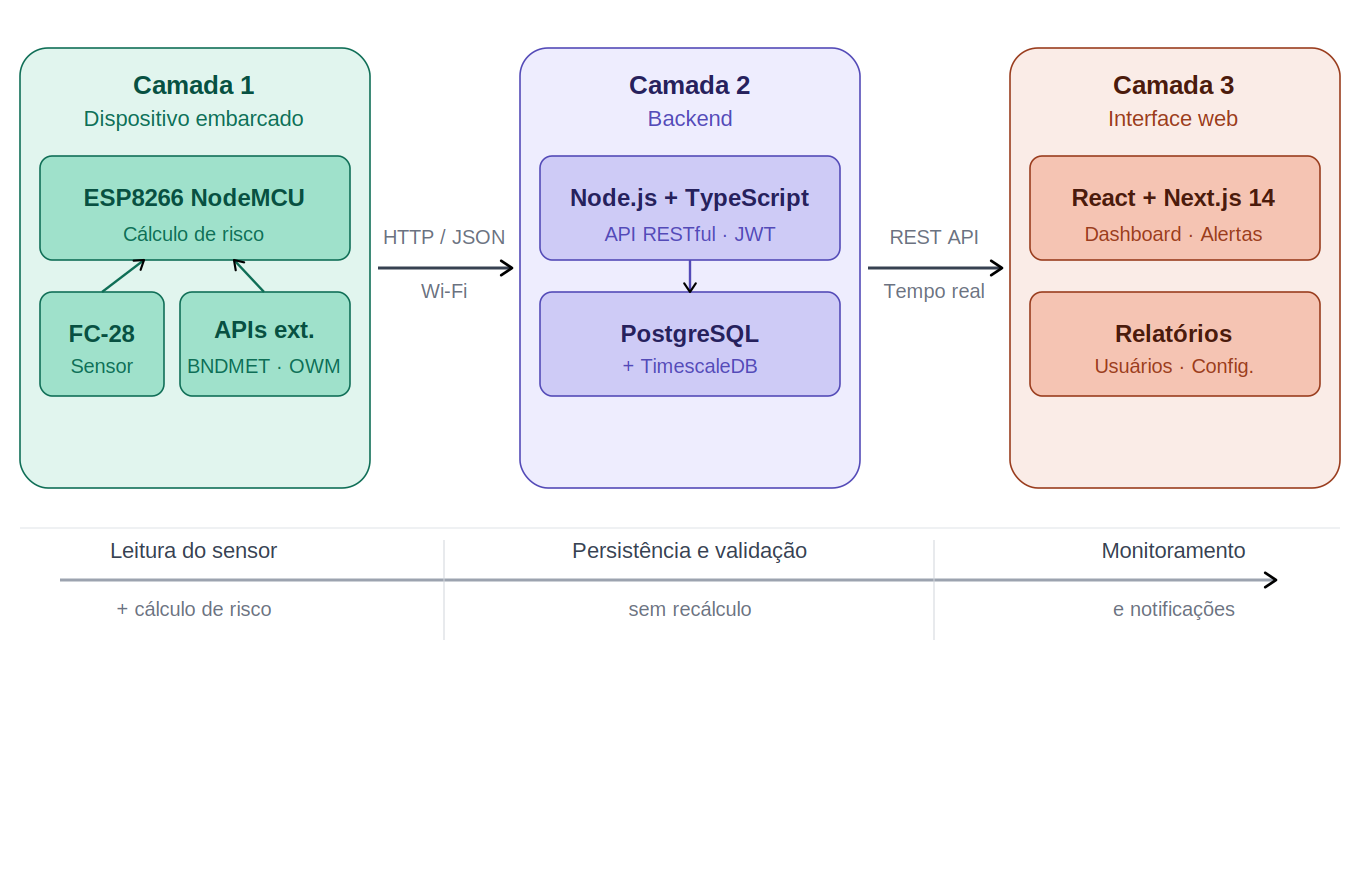
\includegraphics[width=0.95\textwidth]{figures/cap5_arquitetura_sistema.png}
    \caption{Arquitetura de ponta a ponta do sistema: dispositivo embarcado
    ESP8266 com sensor FC-28, \textit{backend} Node.js/PostgreSQL e
    interface \textit{web} React/Next.js.}
    \label{fig:arquitetura_sistema}
    \fonte{Elaborado pela autora.}
\end{figure}

% =============================================================
\section{Dispositivo Embarcado em Operação}
\label{sec:embarcado}
% =============================================================

% -------------------------------------------------------------
\subsection{Inicialização e Testes de Hardware}
\label{subsec:inicializacao}
% -------------------------------------------------------------

Ao ser energizado, o dispositivo embarcado realiza uma sequência de
verificações antes de declarar-se operacional. As
\autoref{fig:prototipo_hardware_pt1} e \autoref{fig:prototipo_hardware_pt2}
exibem o protótipo montado com seus cinco componentes: o ESP8266 NodeMCU
ao centro, o sensor FC-28 com sonda à esquerda, os três LEDs indicadores
(azul, amarelo e vermelho) no topo e o \textit{buzzer} passivo à direita.

\begin{figure}[htbp]
    \centering
    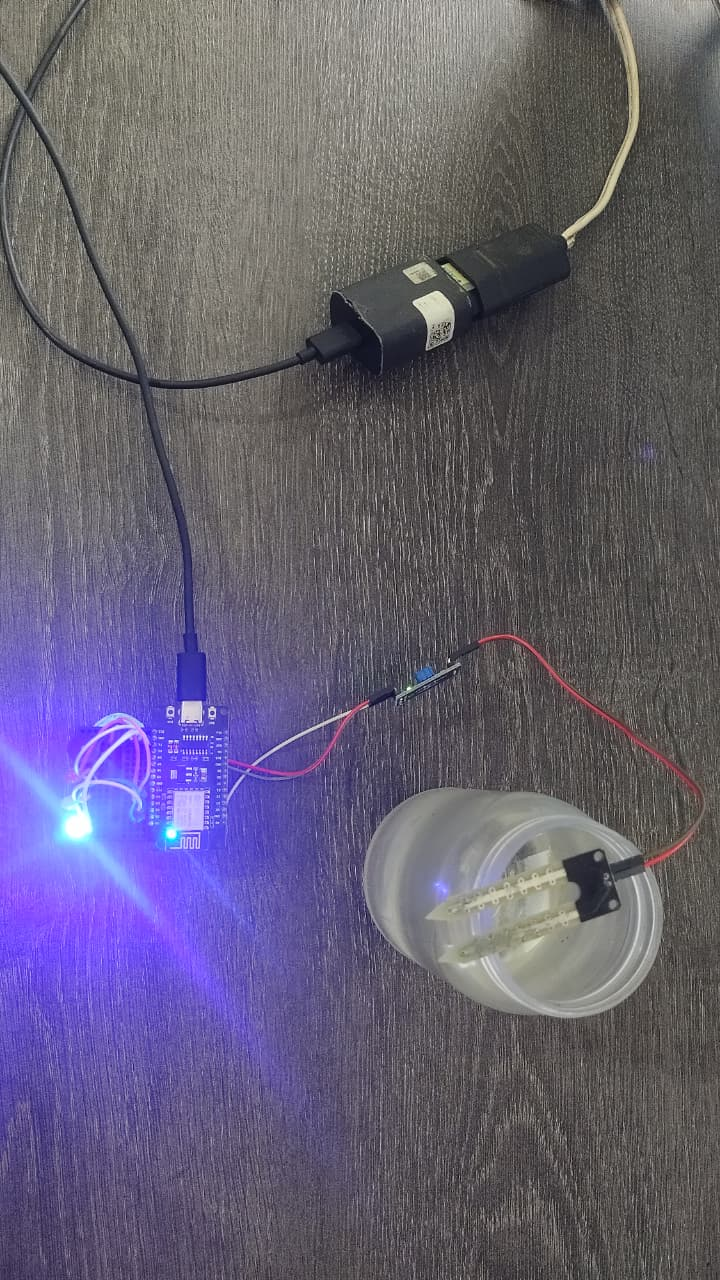
\includegraphics[angle=90, width=0.75\textwidth]{figures/cap5_prototipo_hardware_pt1.jpeg}
    \caption{Protótipo de \textit{hardware} embarcado montado (parte~1): visão
    geral do conjunto com ESP8266 NodeMCU, sensor FC-28 com sonda, LEDs
    indicadores azul, amarelo e vermelho, e \textit{buzzer} passivo.}
    \label{fig:prototipo_hardware_pt1}
    \fonte{Elaborado pela autora.}
\end{figure}

\begin{figure}[htbp]
    \centering
    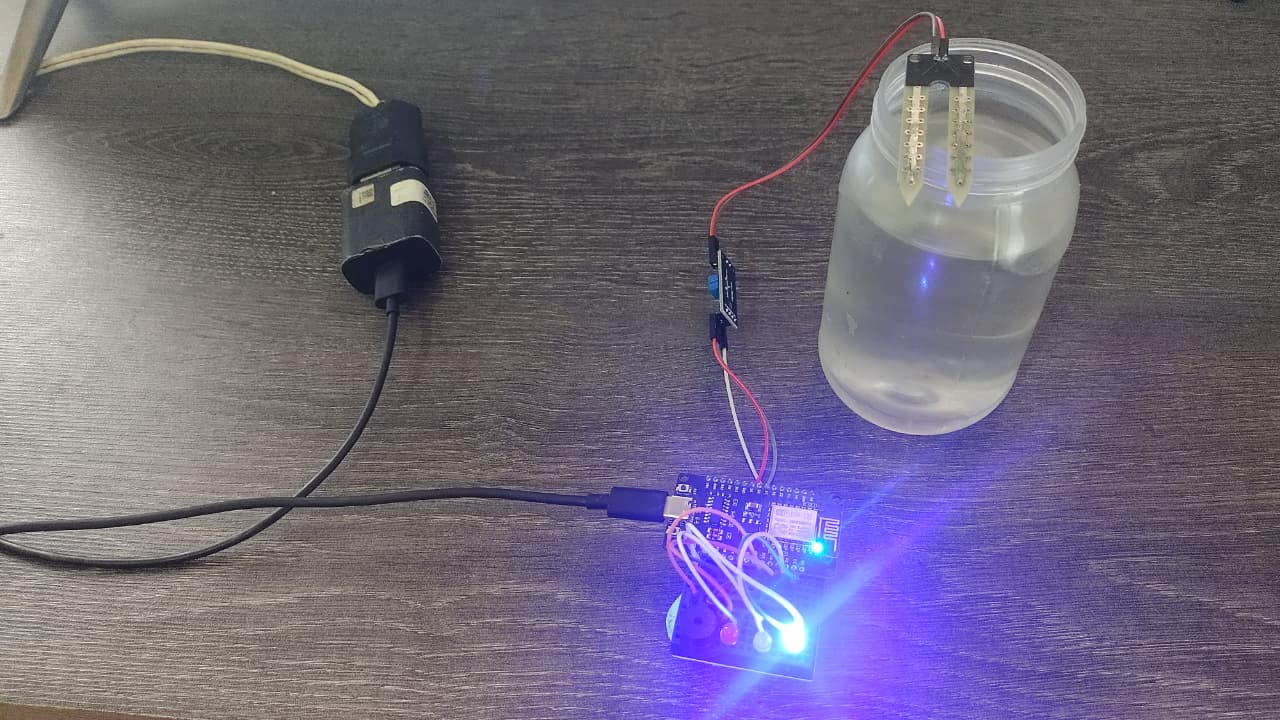
\includegraphics[width=0.75\textwidth]{figures/cap5_prototipo_hardware_pt2.jpeg}
    \caption{Protótipo de \textit{hardware} embarcado montado (parte~2): detalhe
    das conexões entre os componentes.}
    \label{fig:prototipo_hardware_pt2}
    \fonte{Elaborado pela autora.}
\end{figure}

No monitor serial do Arduino IDE, o início da sequência de inicialização
exibe o banner de identificação do sistema, seguido da leitura dos valores
de calibração armazenados na memória EEPROM --- confirmando os pontos de
referência do sensor em solo seco e em solo saturado. Em seguida, os três
LEDs são acionados sequencialmente por 400\,ms cada, permitindo verificar
visualmente a integridade de todos os indicadores antes da operação, conforme mostra a
\autoref{fig:serial_inicializacao_pt1}. Ao concluir o teste de
\textit{hardware}, o sistema conecta ao Wi-Fi, sincroniza o horário via
NTP, consulta as APIs externas BNDMET e OWM, conforme registrado nas \autoref{fig:serial_inicializacao_pt2} e \autoref{fig:serial_inicializacao_pt3}. Por
fim, realiza a primeira coleta de dados e declara operacional com a mensagem
``SISTEMA TOTALMENTE INICIADO'', conforme mostra a
\autoref{fig:serial_inicializacao_pt4}.

\begin{figure}[htbp]
    \centering
    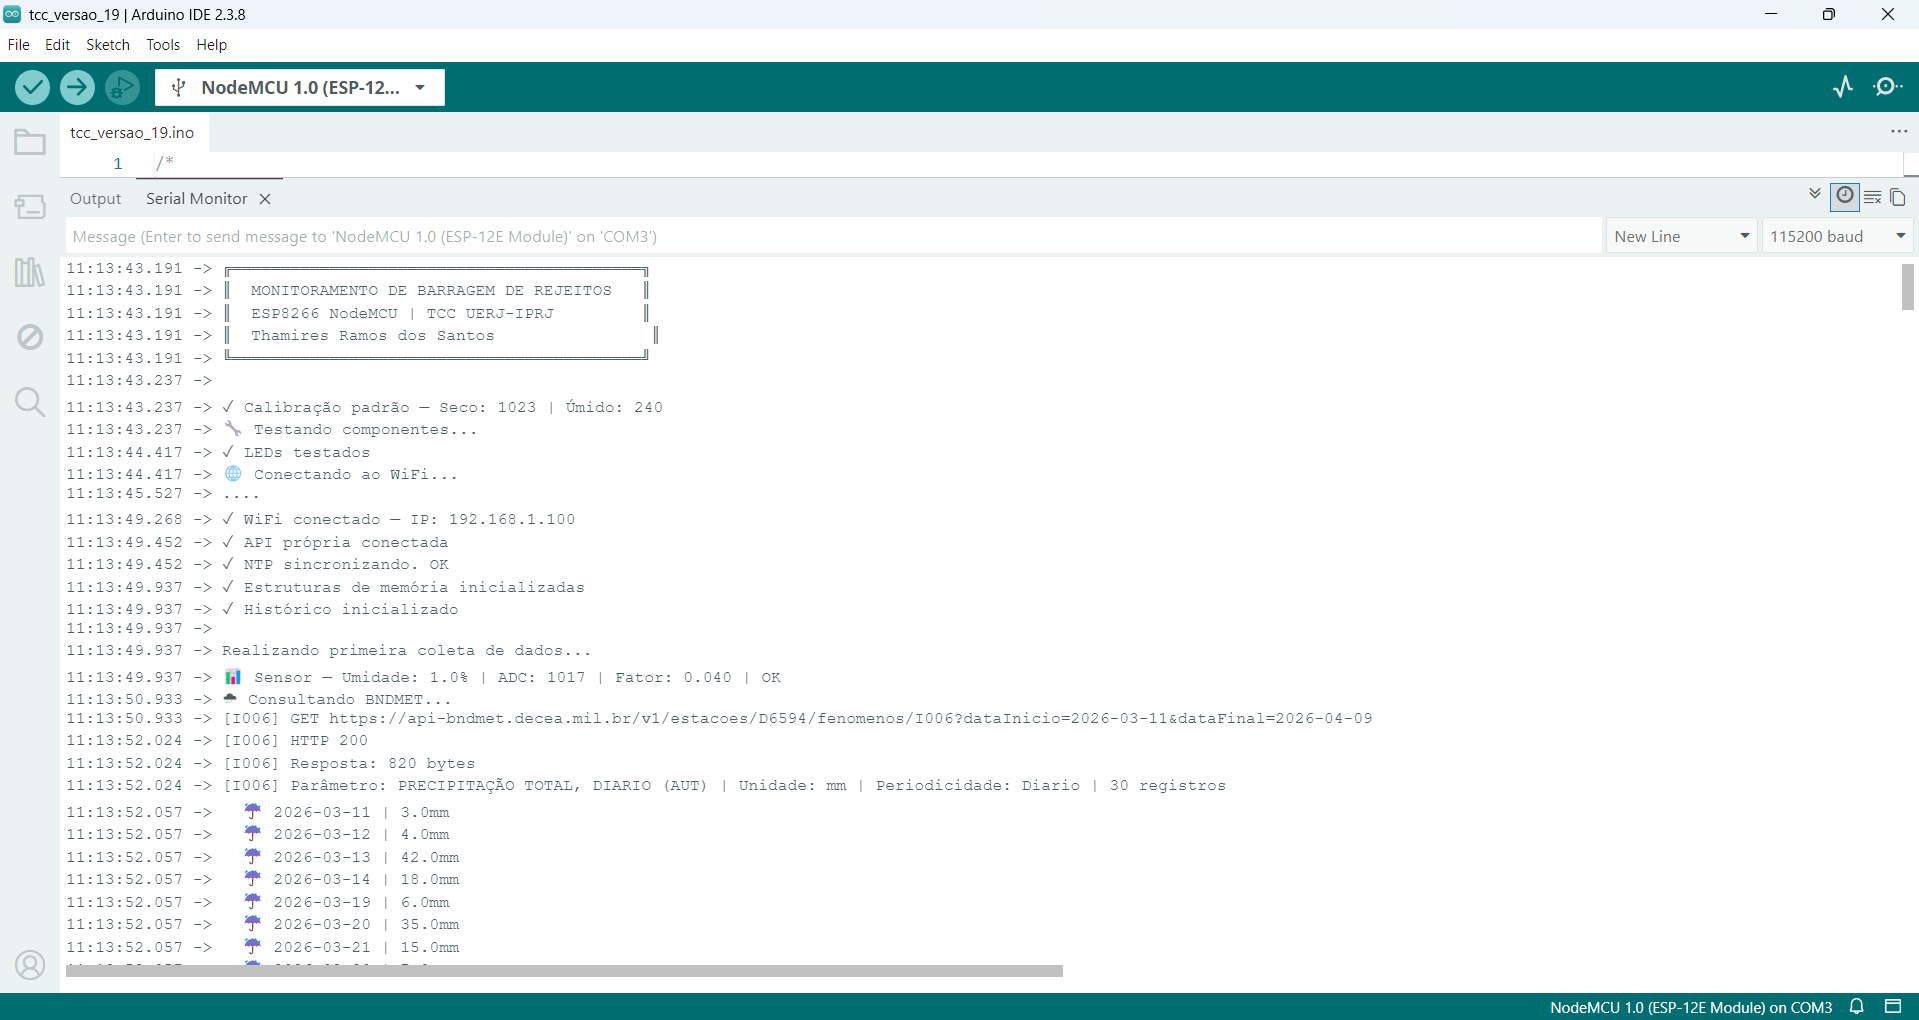
\includegraphics[width=0.85\textwidth]{figures/cap5_serial_inicializacao_pt1.png}
    \caption{Monitor serial durante a inicialização (parte~1): banner de
    identificação do sistema e leitura dos valores de calibração da EEPROM
    para solo seco e solo saturado.}
    \label{fig:serial_inicializacao_pt1}
    \fonte{Elaborado pela autora.}
\end{figure}

\begin{figure}[htbp]
    \centering
    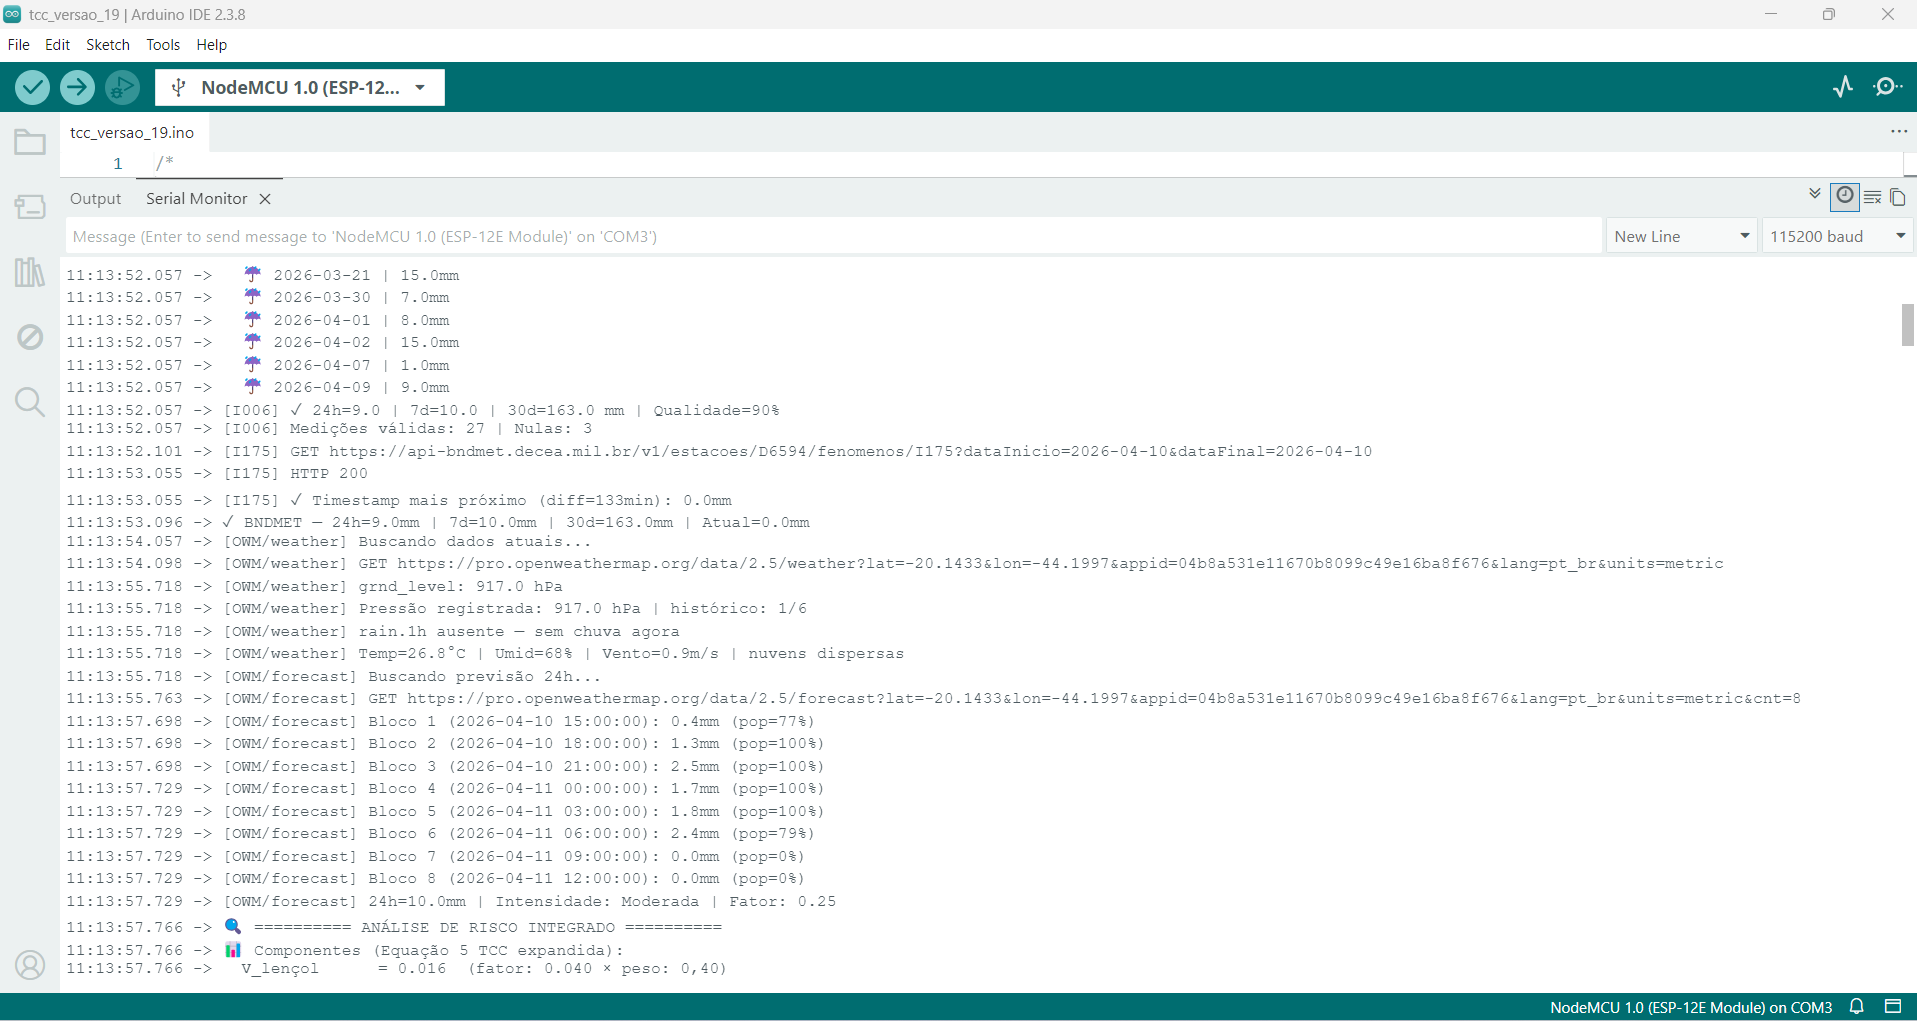
\includegraphics[width=0.85\textwidth]{figures/cap5_serial_inicializacao_pt2.png}
    \caption{Monitor serial durante a inicialização (parte~2): teste
    sequencial dos três LEDs indicadores, acionados por 400\,ms cada para
    verificação visual de integridade.}
    \label{fig:serial_inicializacao_pt2}
    \fonte{Elaborado pela autora.}
\end{figure}

\begin{figure}[htbp]
    \centering
    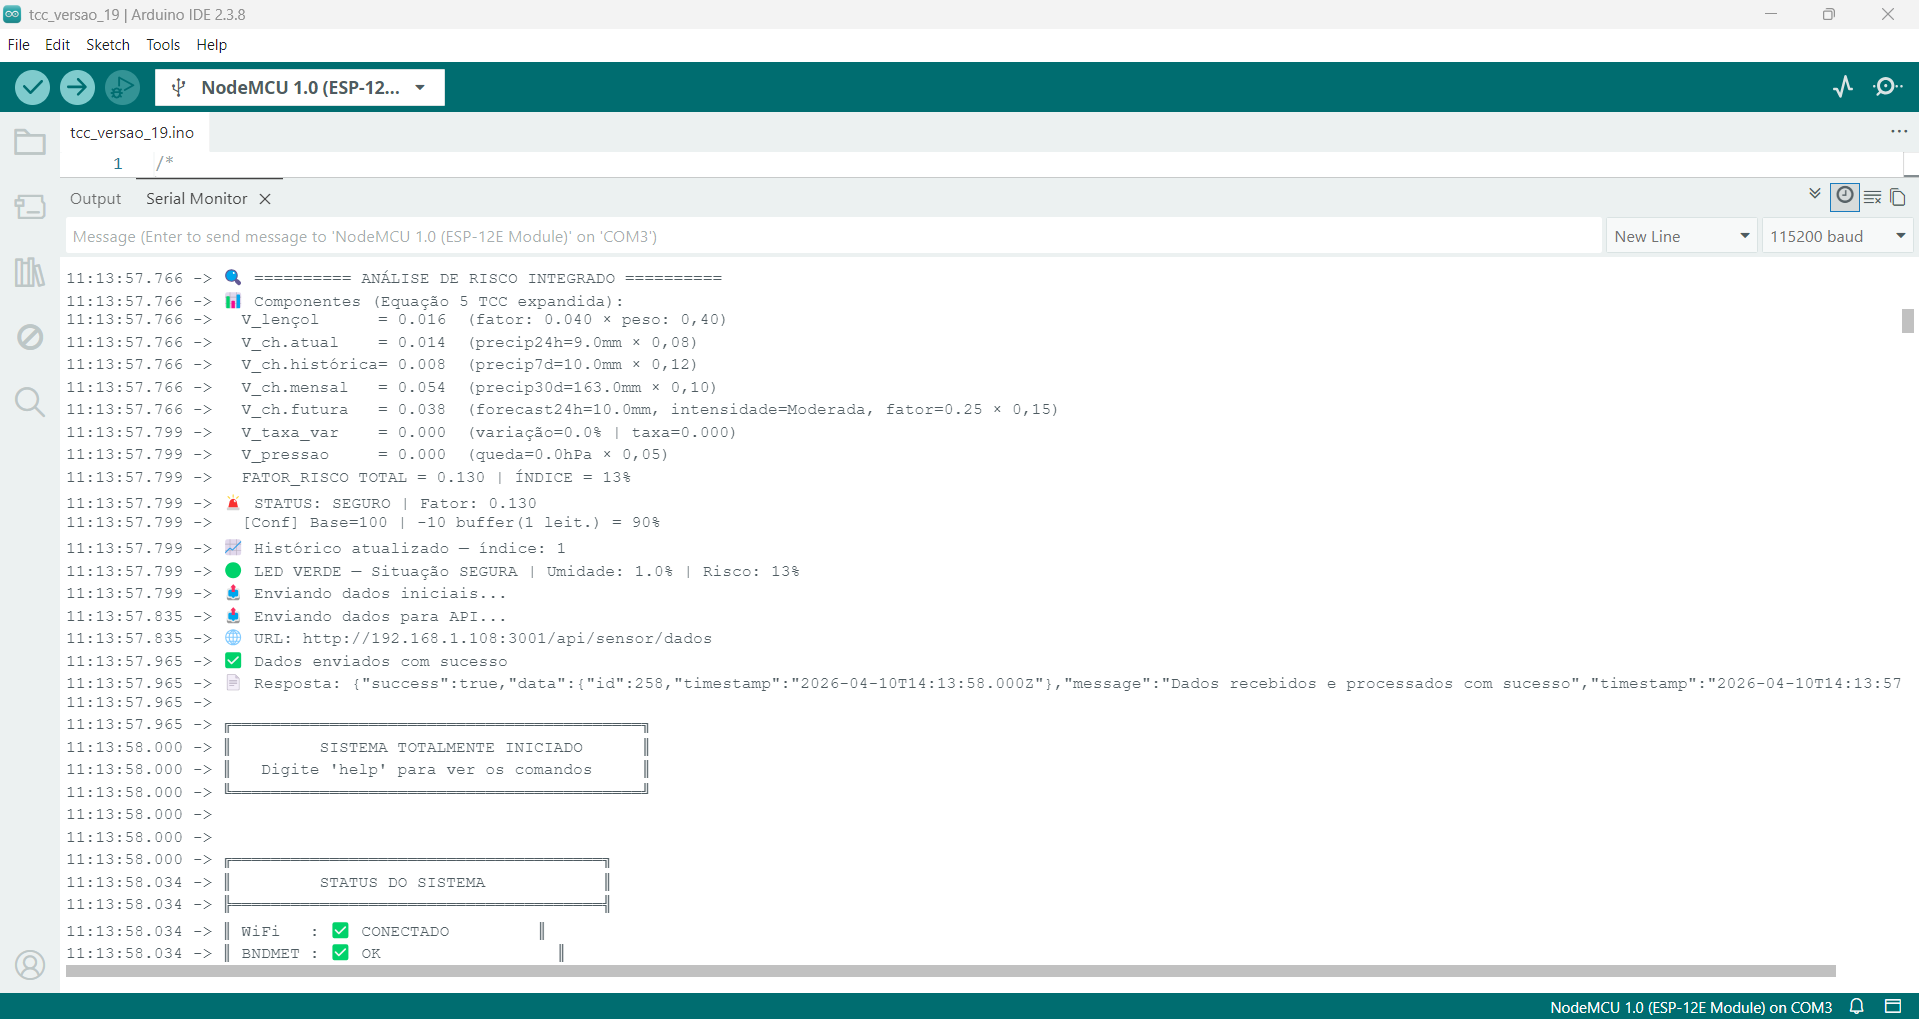
\includegraphics[width=0.85\textwidth]{figures/cap5_serial_inicializacao_pt3.png}
    \caption{Monitor serial durante a inicialização (parte~3): conexão
    Wi-Fi estabelecida, sincronização NTP concluída e consulta as APIs externas BNDMET e OWM.}
    \label{fig:serial_inicializacao_pt3}
    \fonte{Elaborado pela autora.}
\end{figure}

\begin{figure}[htbp]
    \centering
    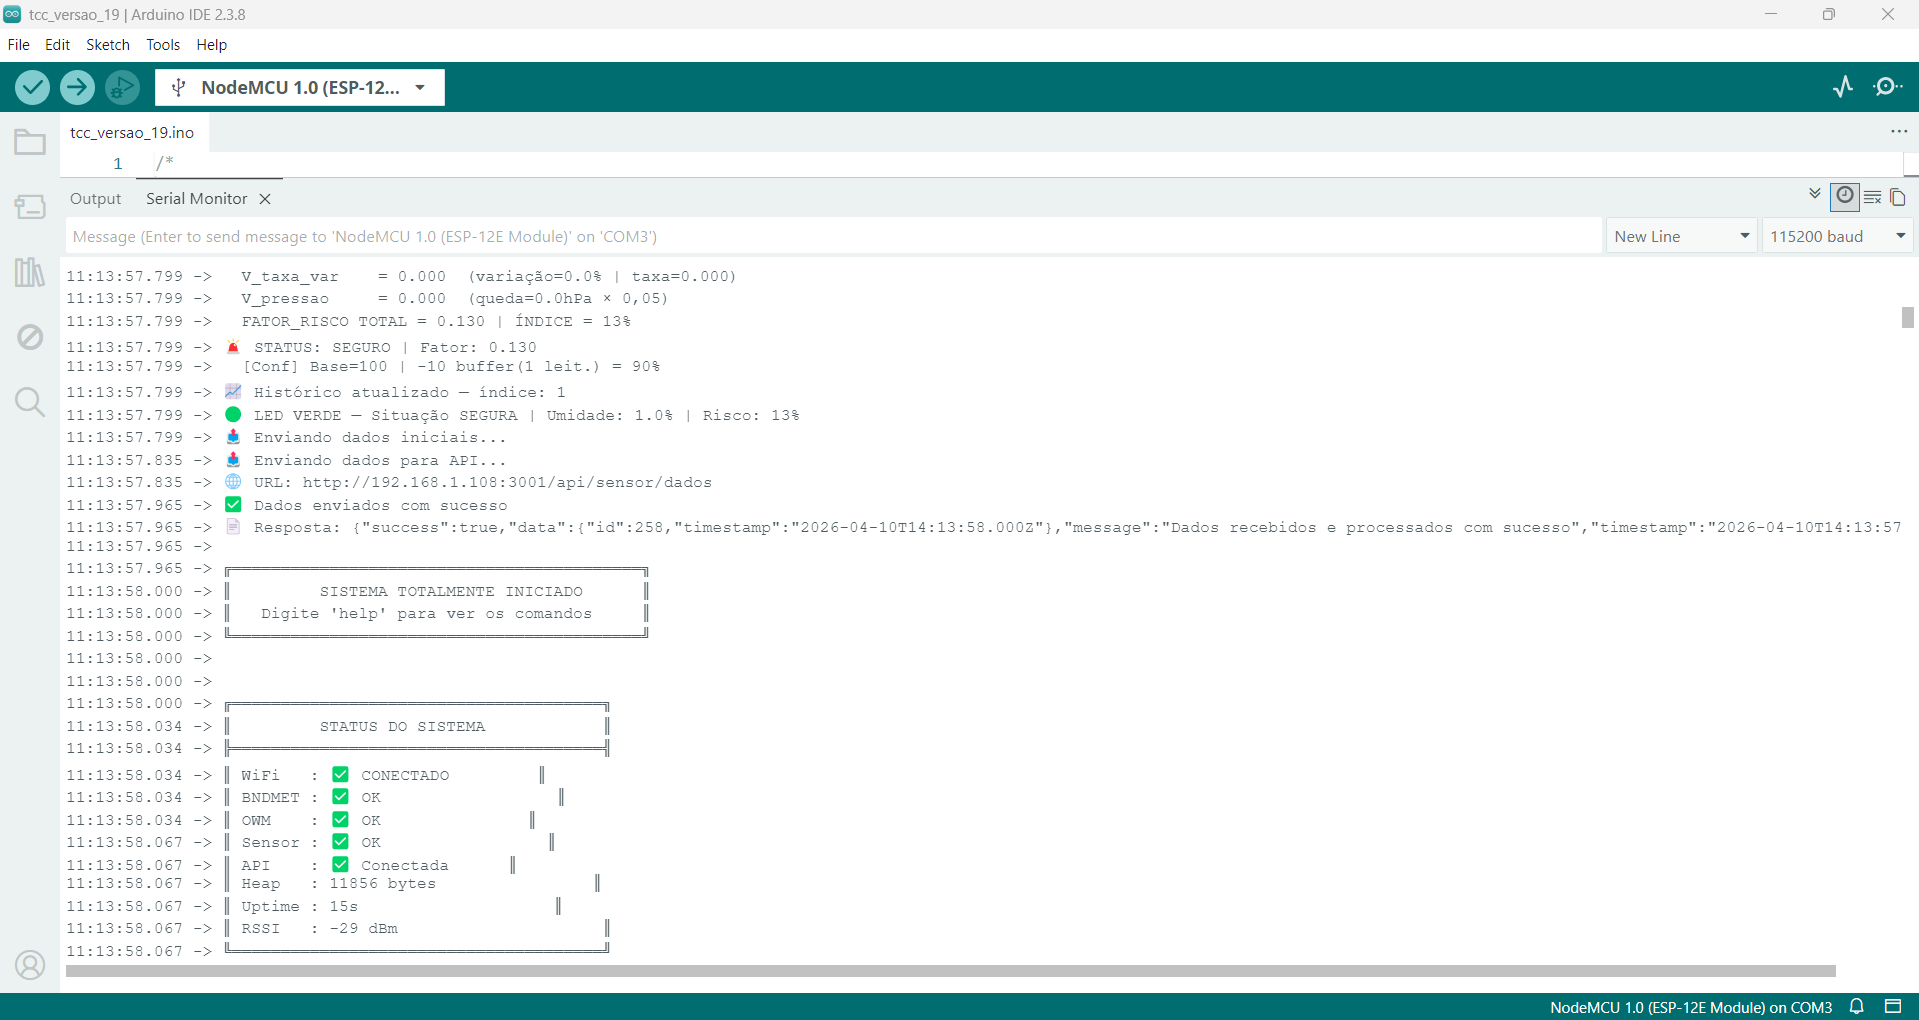
\includegraphics[width=0.85\textwidth]{figures/cap5_serial_inicializacao_pt4.png}
    \caption{Monitor serial durante a inicialização (parte~4): primeira
    coleta de dados realizada e sistema declarado operacional com a mensagem
    ``SISTEMA TOTALMENTE INICIADO''.}
    \label{fig:serial_inicializacao_pt4}
    \fonte{Elaborado pela autora.}
\end{figure}

Quando o \textit{backend} está inacessível no momento da inicialização,
o sistema registra a falha no monitor serial, mantém a variável de
controle de API como inativa e prossegue normalmente em modo local, sem
travar a execução. As leituras continuam sendo realizadas e o cálculo
de risco é executado normalmente; o envio ao banco de dados retomará
assim que a conectividade for restabelecida. De forma análoga, se a
conexão Wi-Fi não for estabelecida após as tentativas iniciais, o
dispositivo opera em modo local, calculando o risco com os dados
disponíveis em memória e aguardando reconexão automática a cada 30
segundos, conforme ilustram as \autoref{fig:serial_backend_inacessivel_pt1}
e \autoref{fig:serial_backend_inacessivel_pt2}.

\begin{figure}[htbp]
    \centering
    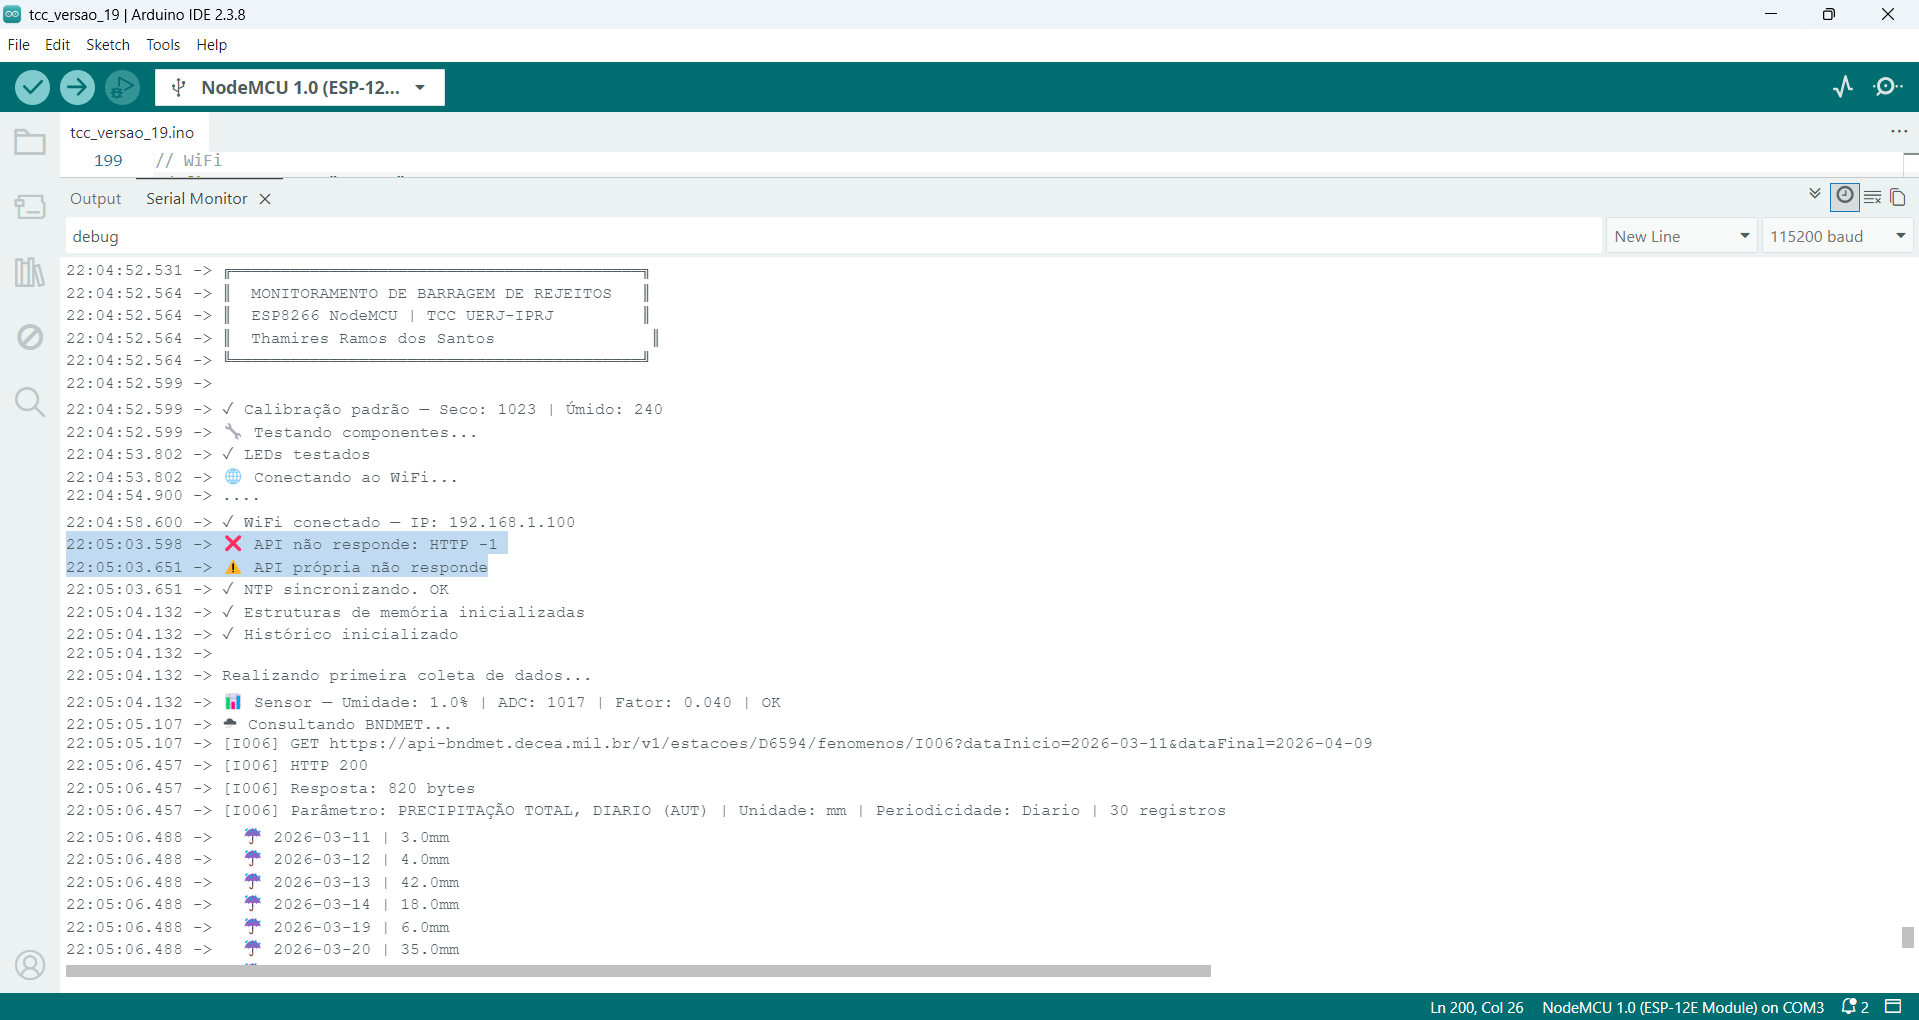
\includegraphics[width=0.85\textwidth]{figures/cap5_serial_backend_inacessivel_pt1.png}
    \caption{Monitor serial durante inicialização com \textit{backend} inacessível (parte~1): falha de conexão registrada e variável de controle da API definida como inativa.}
    \label{fig:serial_backend_inacessivel_pt1}
    \fonte{Elaborado pela autora.}
\end{figure}

\begin{figure}[htbp]
    \centering
    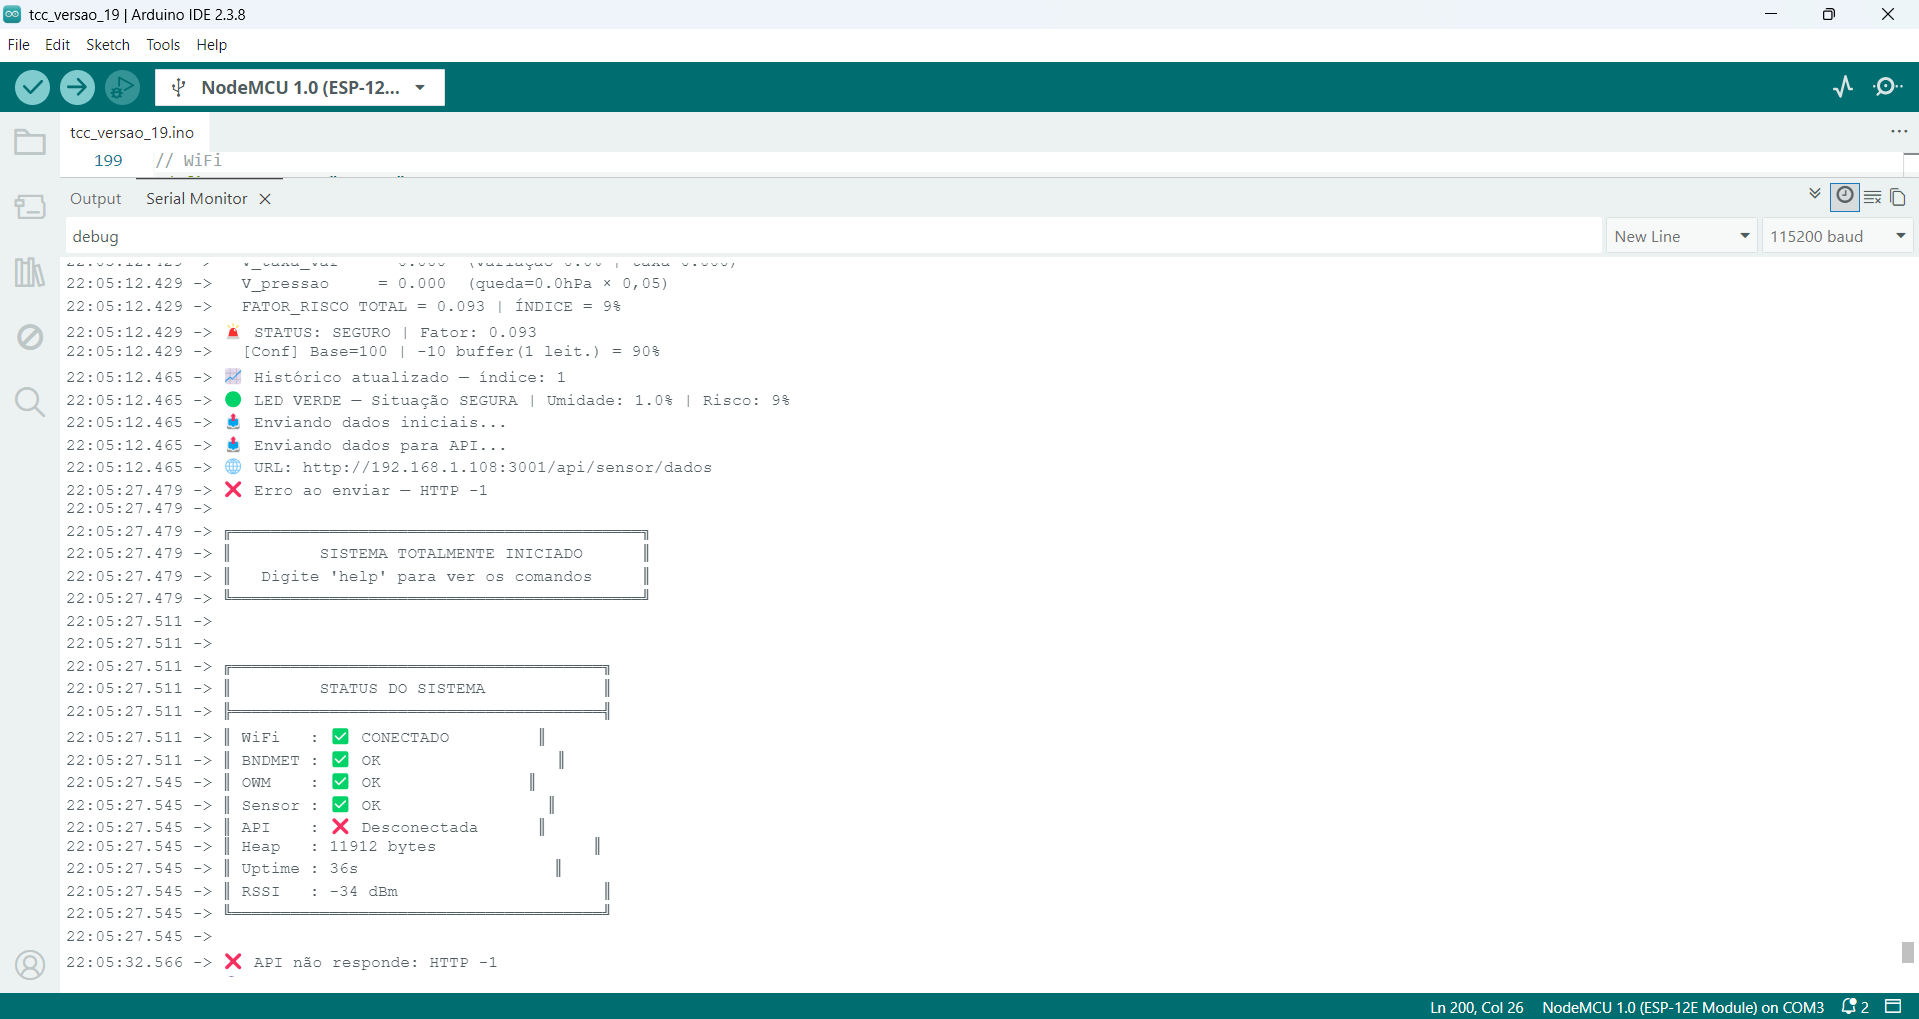
\includegraphics[width=0.85\textwidth]{figures/cap5_serial_backend_inacessivel_pt2.png}
    \caption{Monitor serial durante inicialização com \textit{backend} inacessível (parte~2): sistema prosseguindo em modo local sem interromper a execução.}
    \label{fig:serial_backend_inacessivel_pt2}
    \fonte{Elaborado pela autora.}
\end{figure}

Quando a rede Wi-Fi está inacessível após as tentativas iniciais, o comportamento observado no monitor serial é distinto: o sistema registra cada tentativa malsucedida e, ao esgotar o limite, declara operação em modo local, conforme ilustram as \autoref{fig:serial_wifi_sem_conexao_pt1} e \autoref{fig:serial_wifi_sem_conexao_pt2}.

\begin{figure}[htbp]
    \centering
    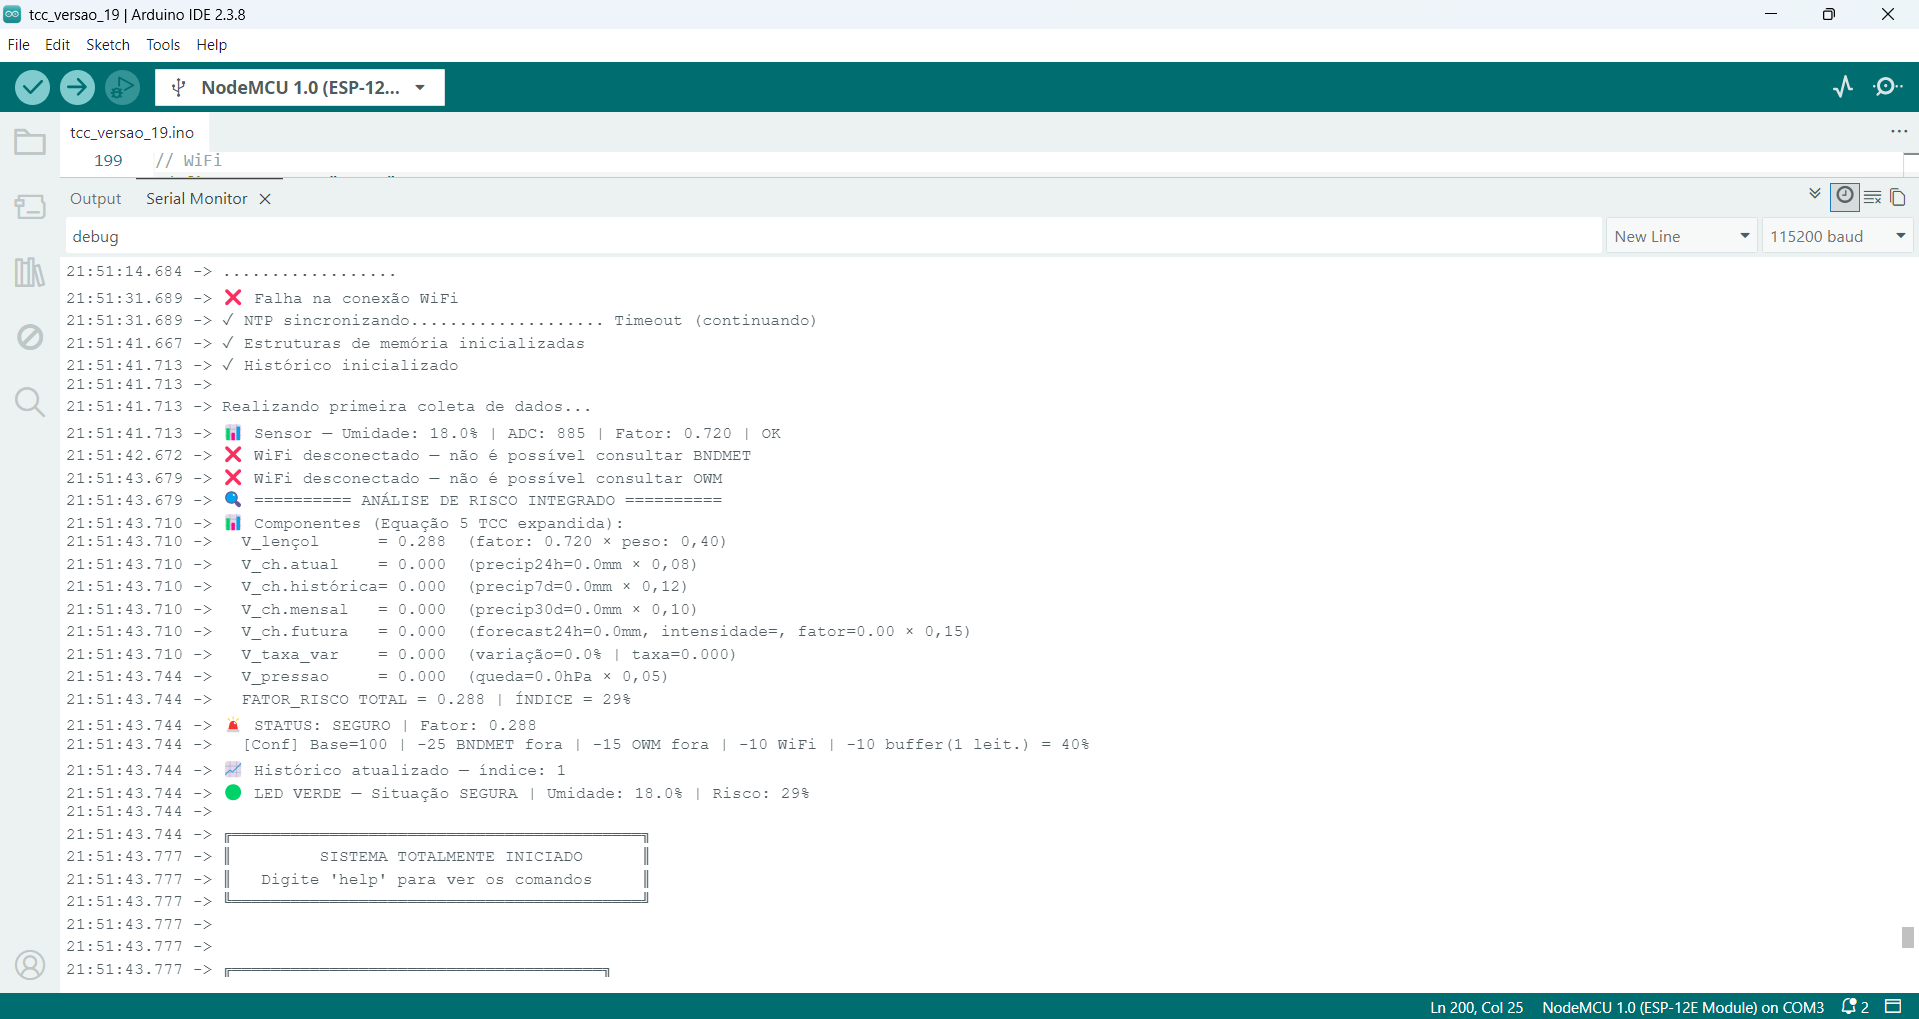
\includegraphics[width=0.85\textwidth]{figures/cap5_serial_wifi_sem_conexao_pt1.png}
    \caption{Monitor serial com Wi-Fi inacessível (parte~1): tentativas de conexão malsucedidas registradas sequencialmente.}
    \label{fig:serial_wifi_sem_conexao_pt1}
    \fonte{Elaborado pela autora.}
\end{figure}

\begin{figure}[htbp]
    \centering
    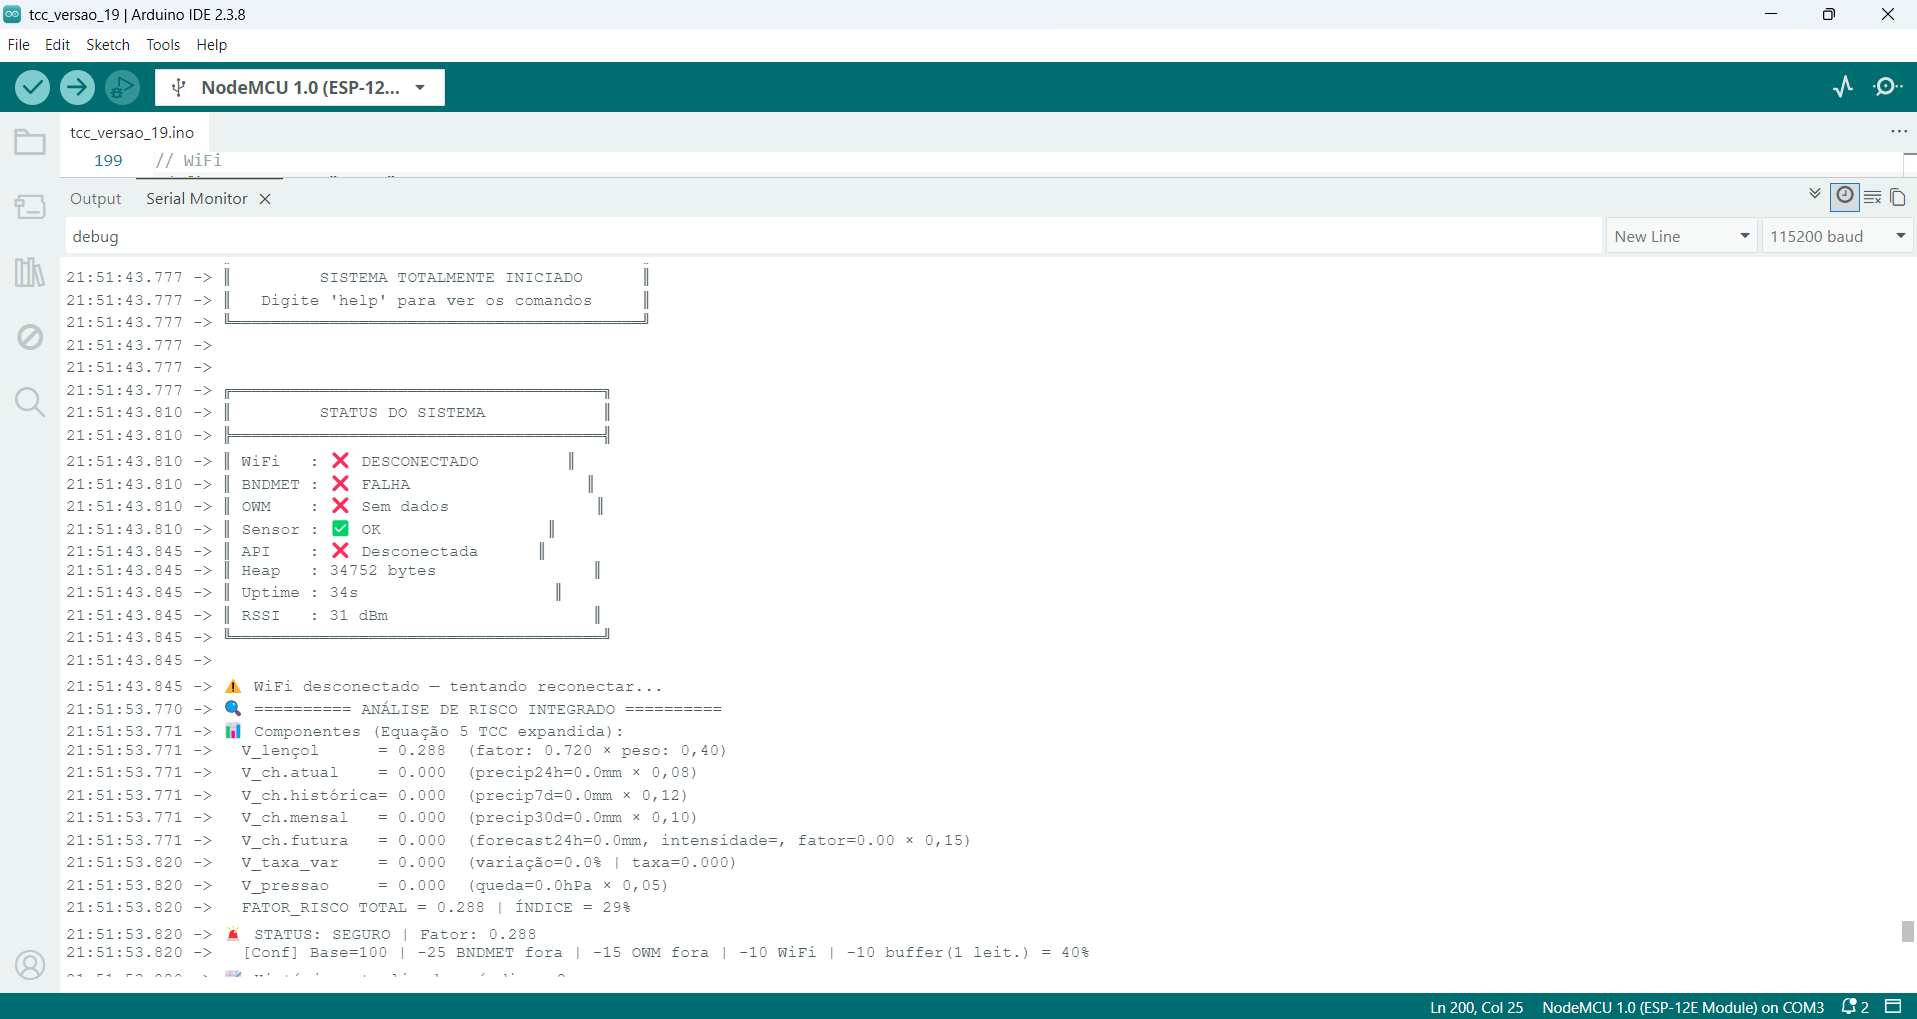
\includegraphics[width=0.85\textwidth]{figures/cap5_serial_wifi_sem_conexao_pt2.png}
    \caption{Monitor serial com Wi-Fi inacessível (parte~2): sistema declarando operação em modo local após esgotar o limite de tentativas, com leituras acumuladas em memória para envio posterior.}
    \label{fig:serial_wifi_sem_conexao_pt2}
    \fonte{Elaborado pela autora.}
\end{figure}

% -------------------------------------------------------------
\subsection{Leitura do Sensor e Indicadores Visuais}
\label{subsec:sensor-leds}
% -------------------------------------------------------------

A cada ciclo de leitura --- a cada 30 segundos em nível VERDE, 10
segundos em AMARELO e 5 segundos em VERMELHO ou RUPTURA, conforme
modelado na \autoref{subsec:arquitetura} do \autoref{cap:materiais-metodos} --- o
monitor serial exibe o valor bruto do conversor analógico-digital, a
umidade calculada em porcentagem, o fator do lençol freático normalizado
e a confirmação de que o sensor está conectado e operando corretamente,
como ilustra a \autoref{fig:serial_sensor}.

\begin{figure}[htbp]
    \centering
    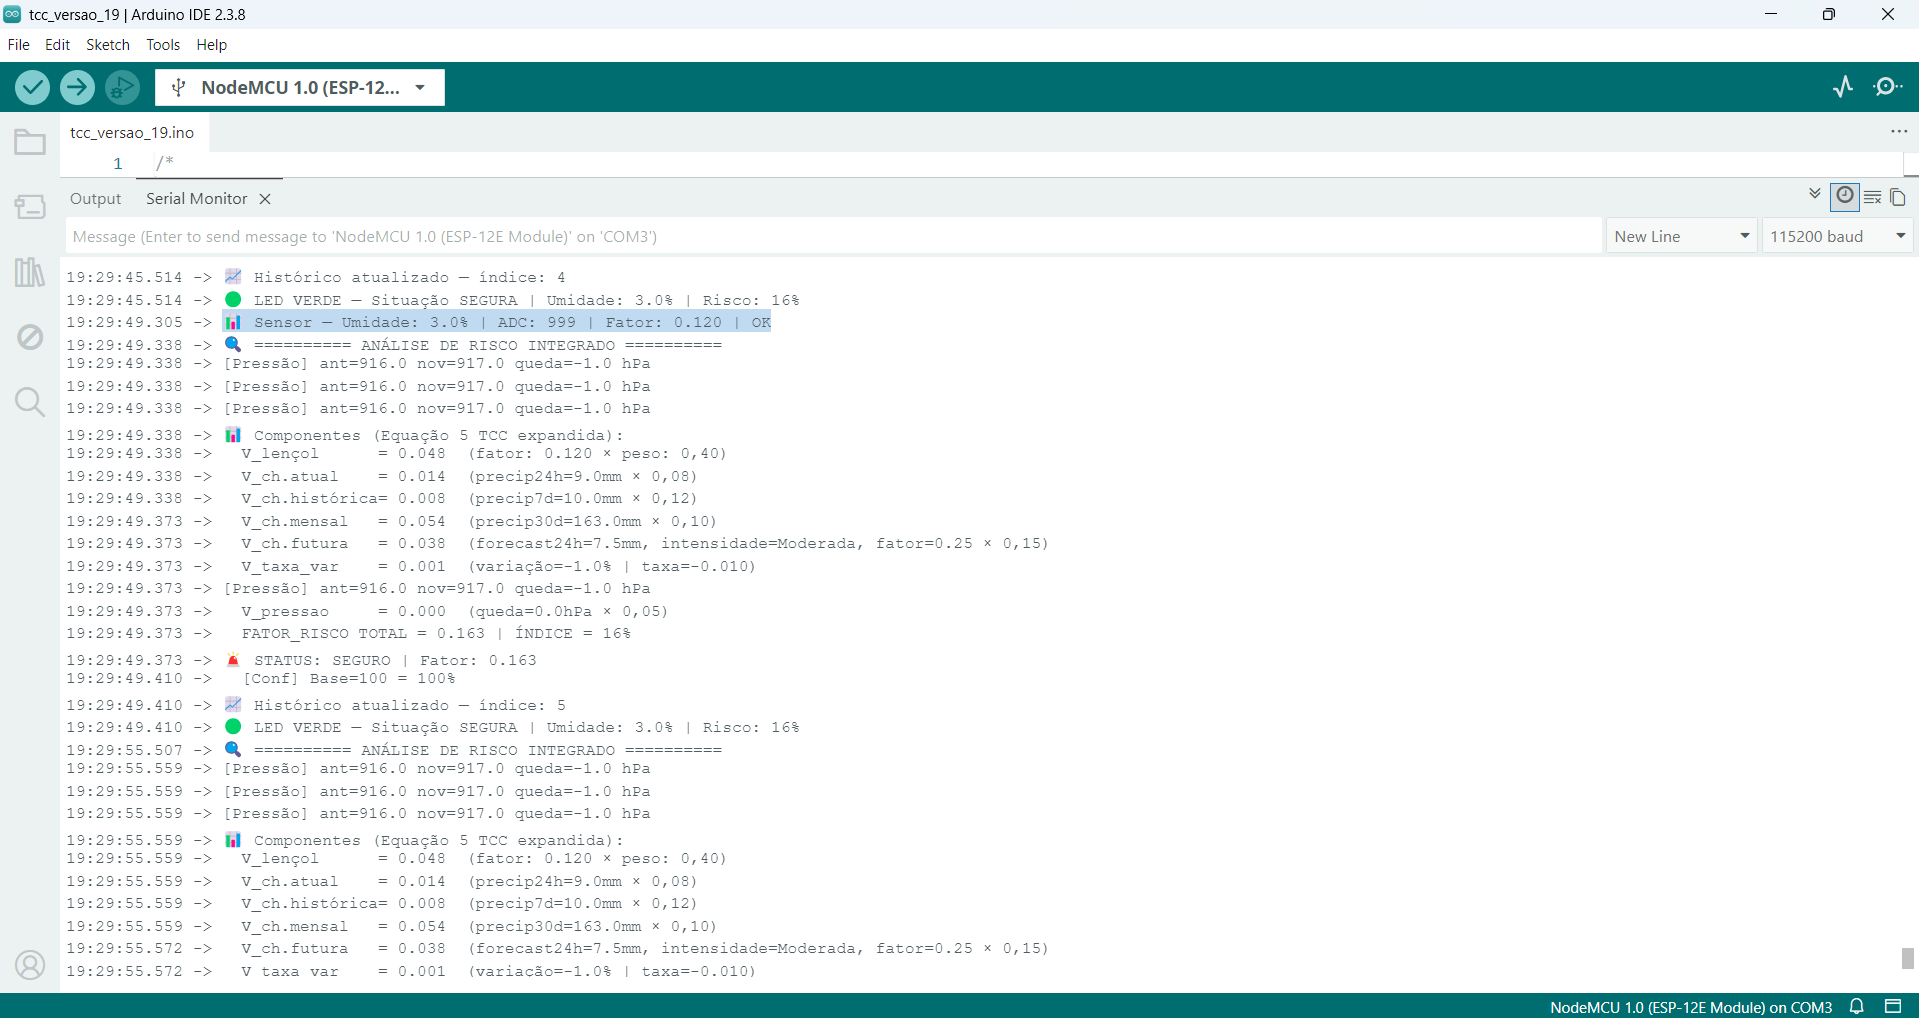
\includegraphics[width=0.85\textwidth]{figures/cap5_serial_sensor.png}
    \caption{Monitor serial durante leitura do sensor FC-28: valor ADC
    bruto, umidade calculada em porcentagem, fator do lençol freático e
    confirmação de \textit{sensorOk}.}
    \label{fig:serial_sensor}
    \fonte{Elaborado pela autora.}
\end{figure}

O LED correspondente ao nível de alerta calculado é acionado ao final de
cada ciclo de análise. A \autoref{fig:leds_niveis} mostra os três estados
visuais do protótipo: LED azul aceso quando o índice de risco não supera
45\% (situação segura), LED amarelo aceso entre 46\% e 75\% (atenção) e
LED vermelho aceso acima de 75\% (situação crítica). Neste último caso,
o \textit{buzzer} também é ativado em modo intermitente, com frequência e
cadência que crescem proporcionalmente à gravidade: 2.000\,Hz com
\textit{beep} a cada 800\,ms entre 75 e 84\%, 2.200\,Hz a cada 500\,ms
entre 85 e 89\%, e 2.400\,Hz a cada 300\,ms para índices iguais ou
superiores a 90\%.

\begin{figure}[htbp]
    \centering
    \includegraphics[width=0.90\textwidth]{figures/cap5_leds_niveis.png}
    \caption{Estados visuais do protótipo: LED azul aceso (nível VERDE,
    situação segura), LED amarelo aceso (nível AMARELO, atenção) e LED
    vermelho aceso com \textit{buzzer} ativo (nível VERMELHO, situação
    crítica).}
    \label{fig:leds_niveis}
    \fonte{Elaborado pela autora.}
\end{figure}

Se o sensor for desconectado ou apresentar curto-circuito, o sistema
identifica a falha, registra \textit{sensorOk} como inativo no monitor
serial e aplica um desconto no índice de confiabilidade da análise.
A detecção é precisa: \texttt{sensorOk} é definido como \texttt{false}
exclusivamente quando o ADC retorna o valor~0 --- indicando
curto-circuito na sonda --- ou o valor~1023 --- indicando circuito
aberto por desconexão. Qualquer leitura intermediária, mesmo que produza
uma umidade calculada duvidosa, é tratada como operação normal pelo
firmware. O cálculo de risco prossegue com os demais componentes
disponíveis, conforme ilustram as \autoref{fig:serial_sensor_falha_pt1}
e \autoref{fig:serial_sensor_falha_pt2}. Quando o administrador acessa
o comando de simulação via monitor serial (\texttt{alerta amarelo} ou
\texttt{alerta vermelho}, por exemplo), o LED correspondente ao nível
forçado acende imediatamente e o intervalo de envio ao \textit{backend}
assume o valor do nível simulado, conforme ilustram a
\autoref{fig:serial_modo_manual} e a \autoref{fig:serial_modo_manual_vermelho}.

\begin{figure}[htbp]
    \centering
    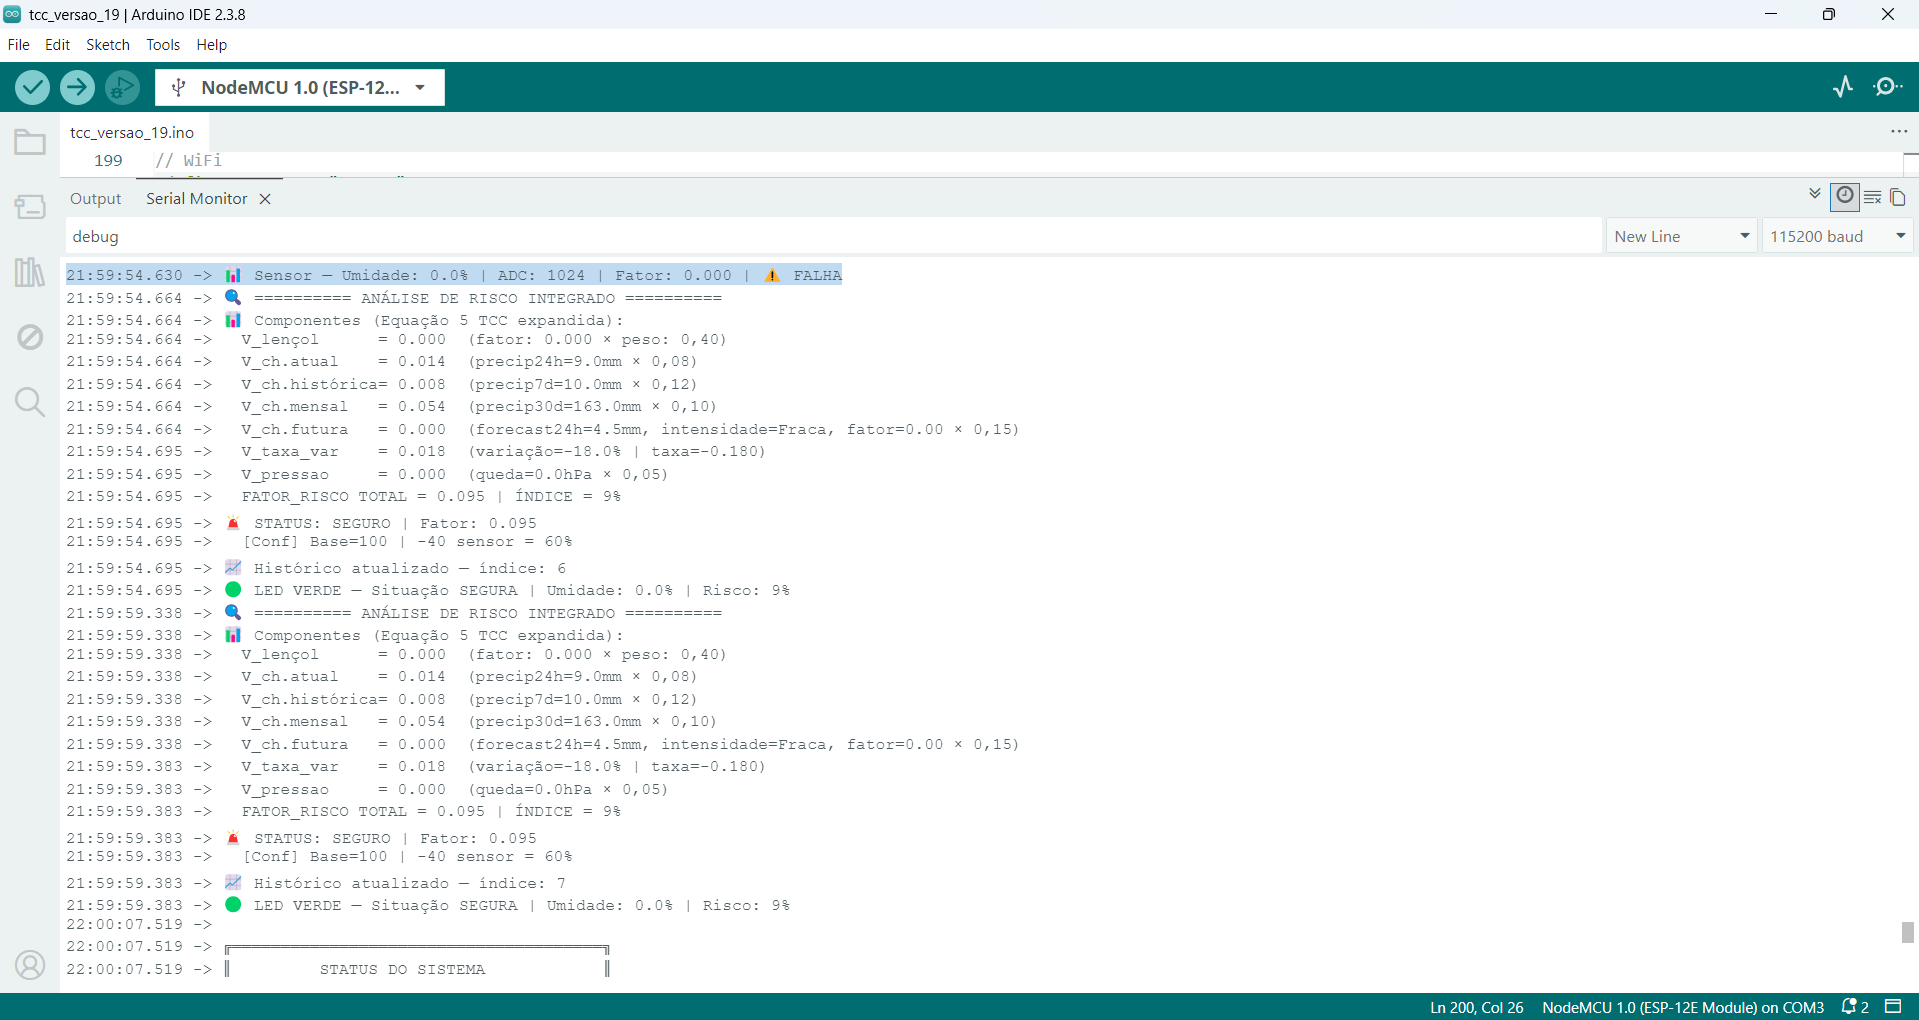
\includegraphics[width=0.85\textwidth]{figures/cap5_serial_sensor_falha_pt1.png}
    \caption{Monitor serial com sensor FC-28 desconectado (parte~1): leitura ADC nos limites do conversor e \textit{sensorOk} registrado como inativo.}
    \label{fig:serial_sensor_falha_pt1}
    \fonte{Elaborado pela autora.}
\end{figure}

\begin{figure}[htbp]
    \centering
    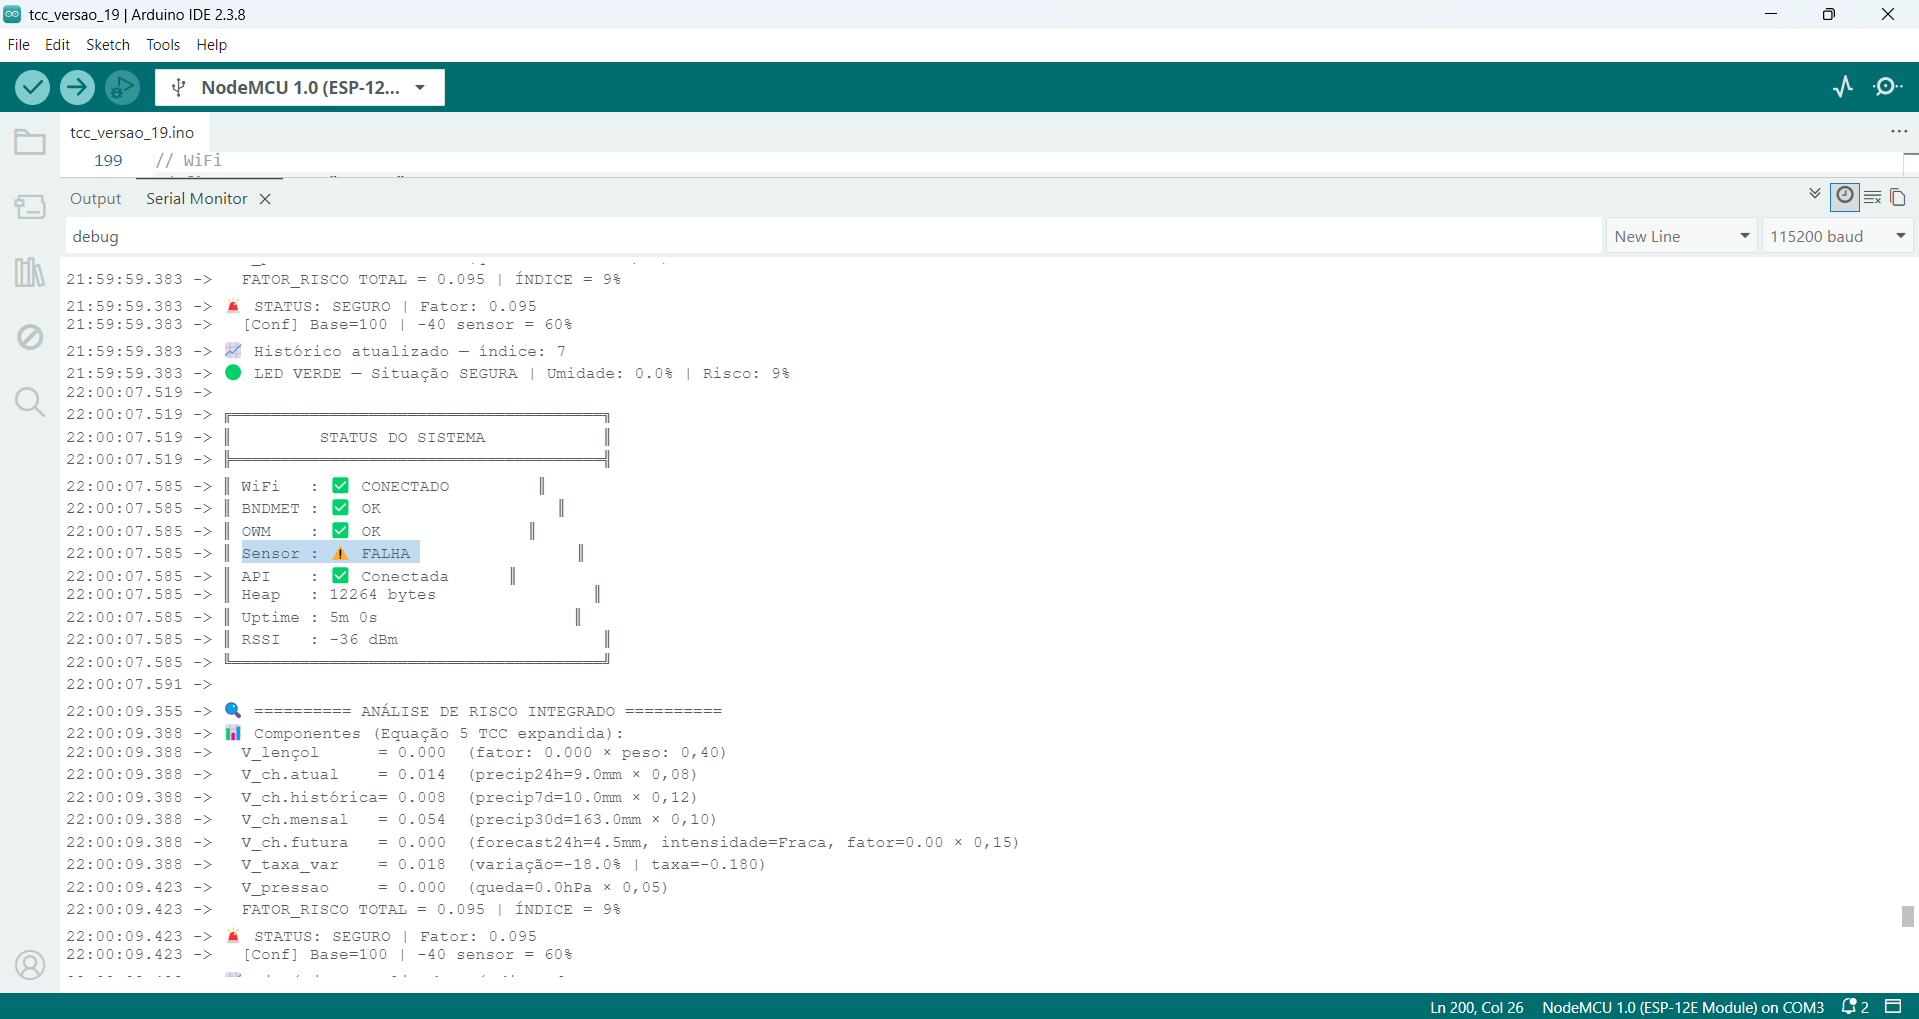
\includegraphics[width=0.85\textwidth]{figures/cap5_serial_sensor_falha_pt2.png}
    \caption{Monitor serial com sensor FC-28 desconectado (parte~2): desconto de 40 pontos aplicado ao índice de confiabilidade; o cálculo de risco prossegue com os demais componentes disponíveis.}
    \label{fig:serial_sensor_falha_pt2}
    \fonte{Elaborado pela autora.}
\end{figure}

\begin{figure}[htbp]
    \centering
    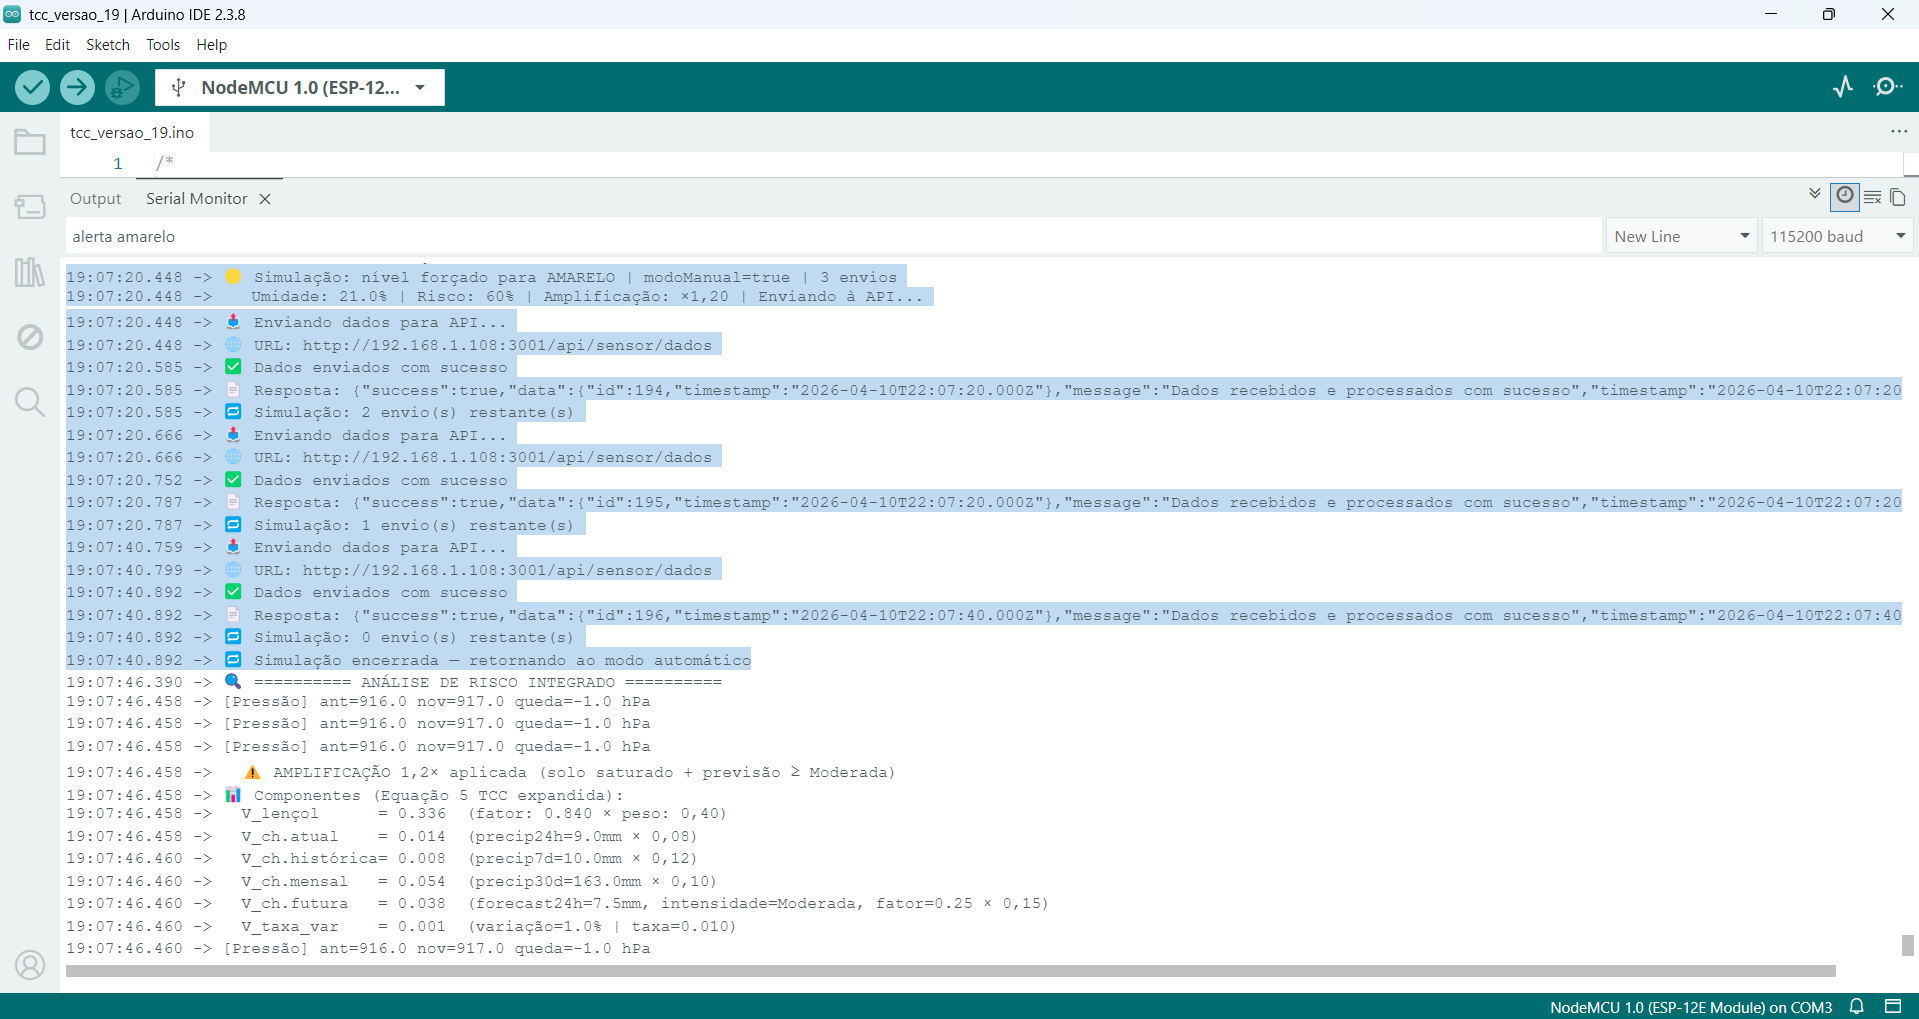
\includegraphics[width=0.85\textwidth]{figures/cap5_serial_modo_manual.png}
    \caption{Monitor serial após execução do comando \texttt{alerta amarelo}: LED amarelo acionado, intervalo de envio ao \textit{backend} ajustado para 20 segundos e nível forçado mantido até a próxima leitura real do sensor.}
    \label{fig:serial_modo_manual}
    \fonte{Elaborado pela autora.}
\end{figure}

\begin{figure}[htbp]
    \centering
    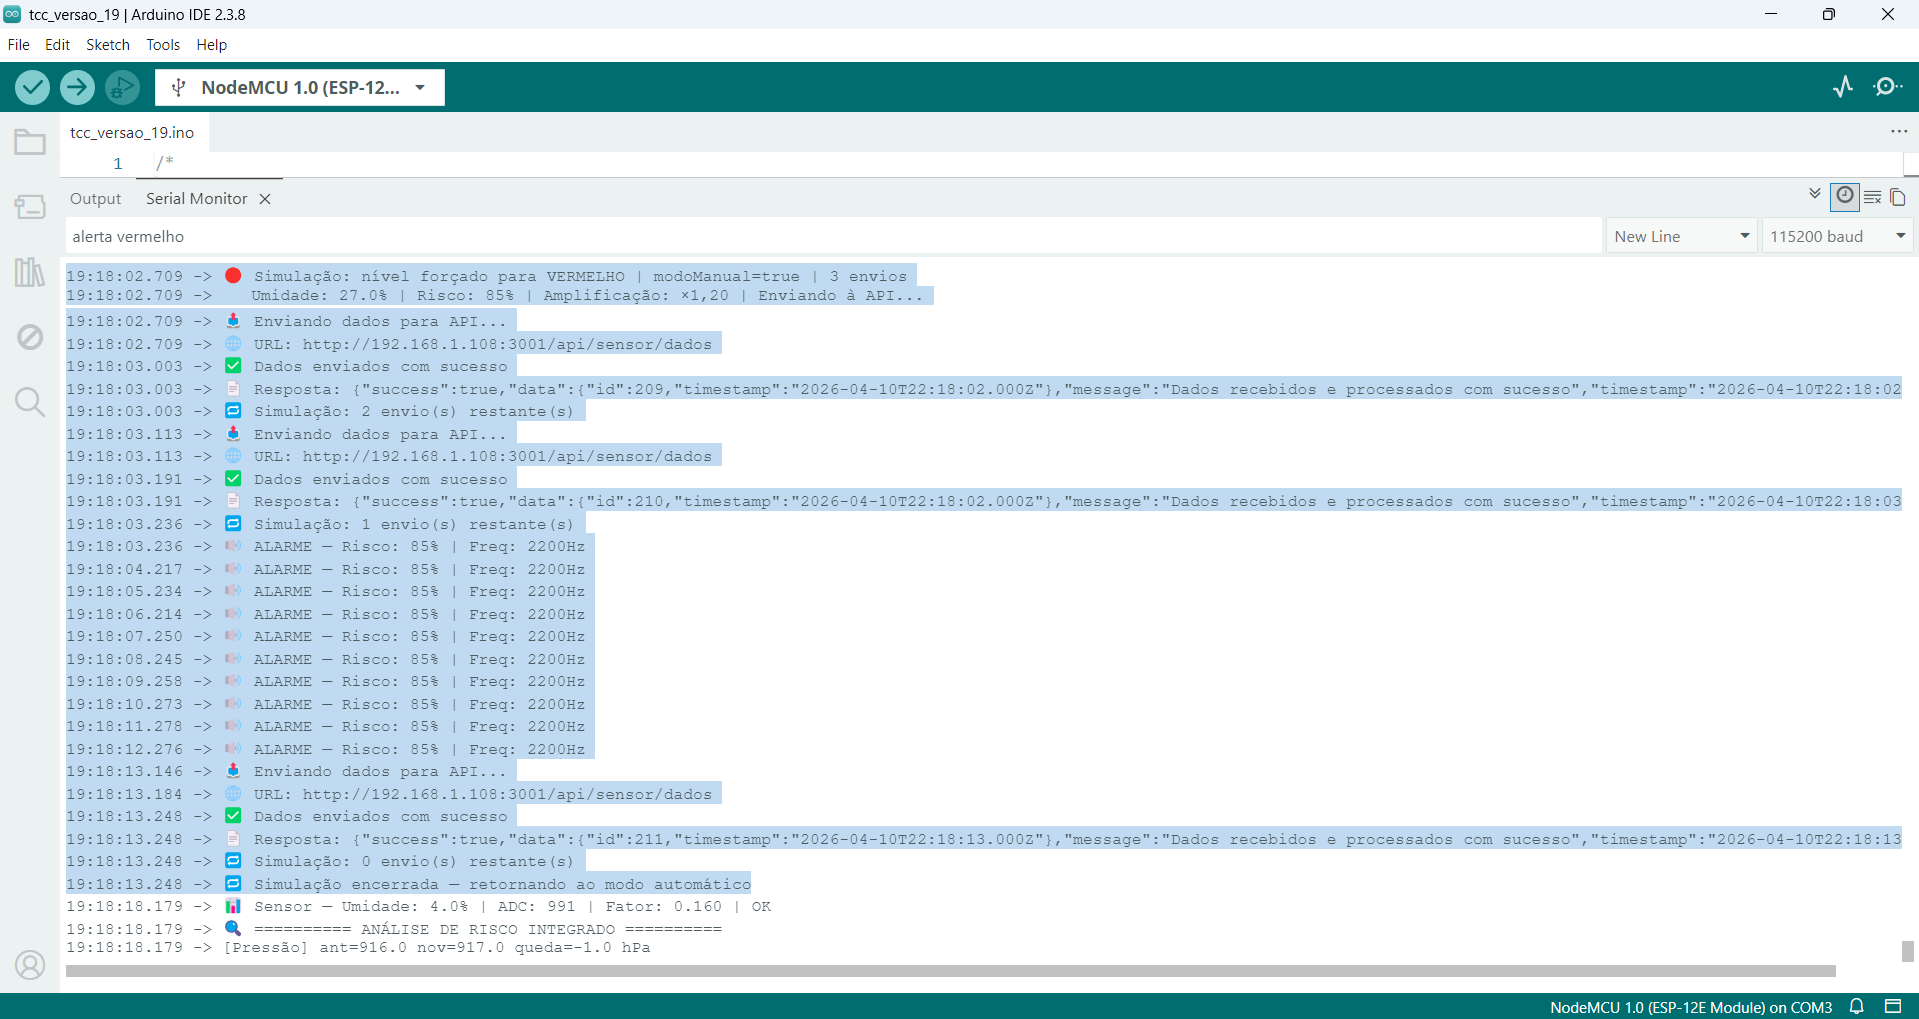
\includegraphics[width=0.85\textwidth]{figures/cap5_serial_modo_manual_vermelho.png}
    \caption{Monitor serial após execução do comando \texttt{alerta vermelho}: LED vermelho acionado, intervalo de envio ao \textit{backend} ajustado para 10 segundos e nível forçado mantido até a próxima leitura real do sensor.}
    \label{fig:serial_modo_manual_vermelho}
    \fonte{Elaborado pela autora.}
\end{figure}

% -------------------------------------------------------------
\subsection{Consultas às APIs Externas e Análise de Risco}
\label{subsec:apis-risco}
% -------------------------------------------------------------

Após cada consulta bem-sucedida à API BNDMET/DECEA, o monitor serial
confirma os acumulados pluviométricos obtidos para as janelas de 24
horas, 7 dias e 30 dias, a precipitação horária atual e o percentual de
qualidade dos dados da estação D6594, conforme a
\autoref{fig:serial_bndmet}. Da mesma forma, ao consultar a
OpenWeatherMap, o sistema exibe a pressão atmosférica, a temperatura,
a chuva atual, o acumulado previsto para as próximas 24 horas e a
classificação de intensidade atribuída ao evento, como mostra a
\autoref{fig:serial_owm}.

\begin{figure}[htbp]
    \centering
    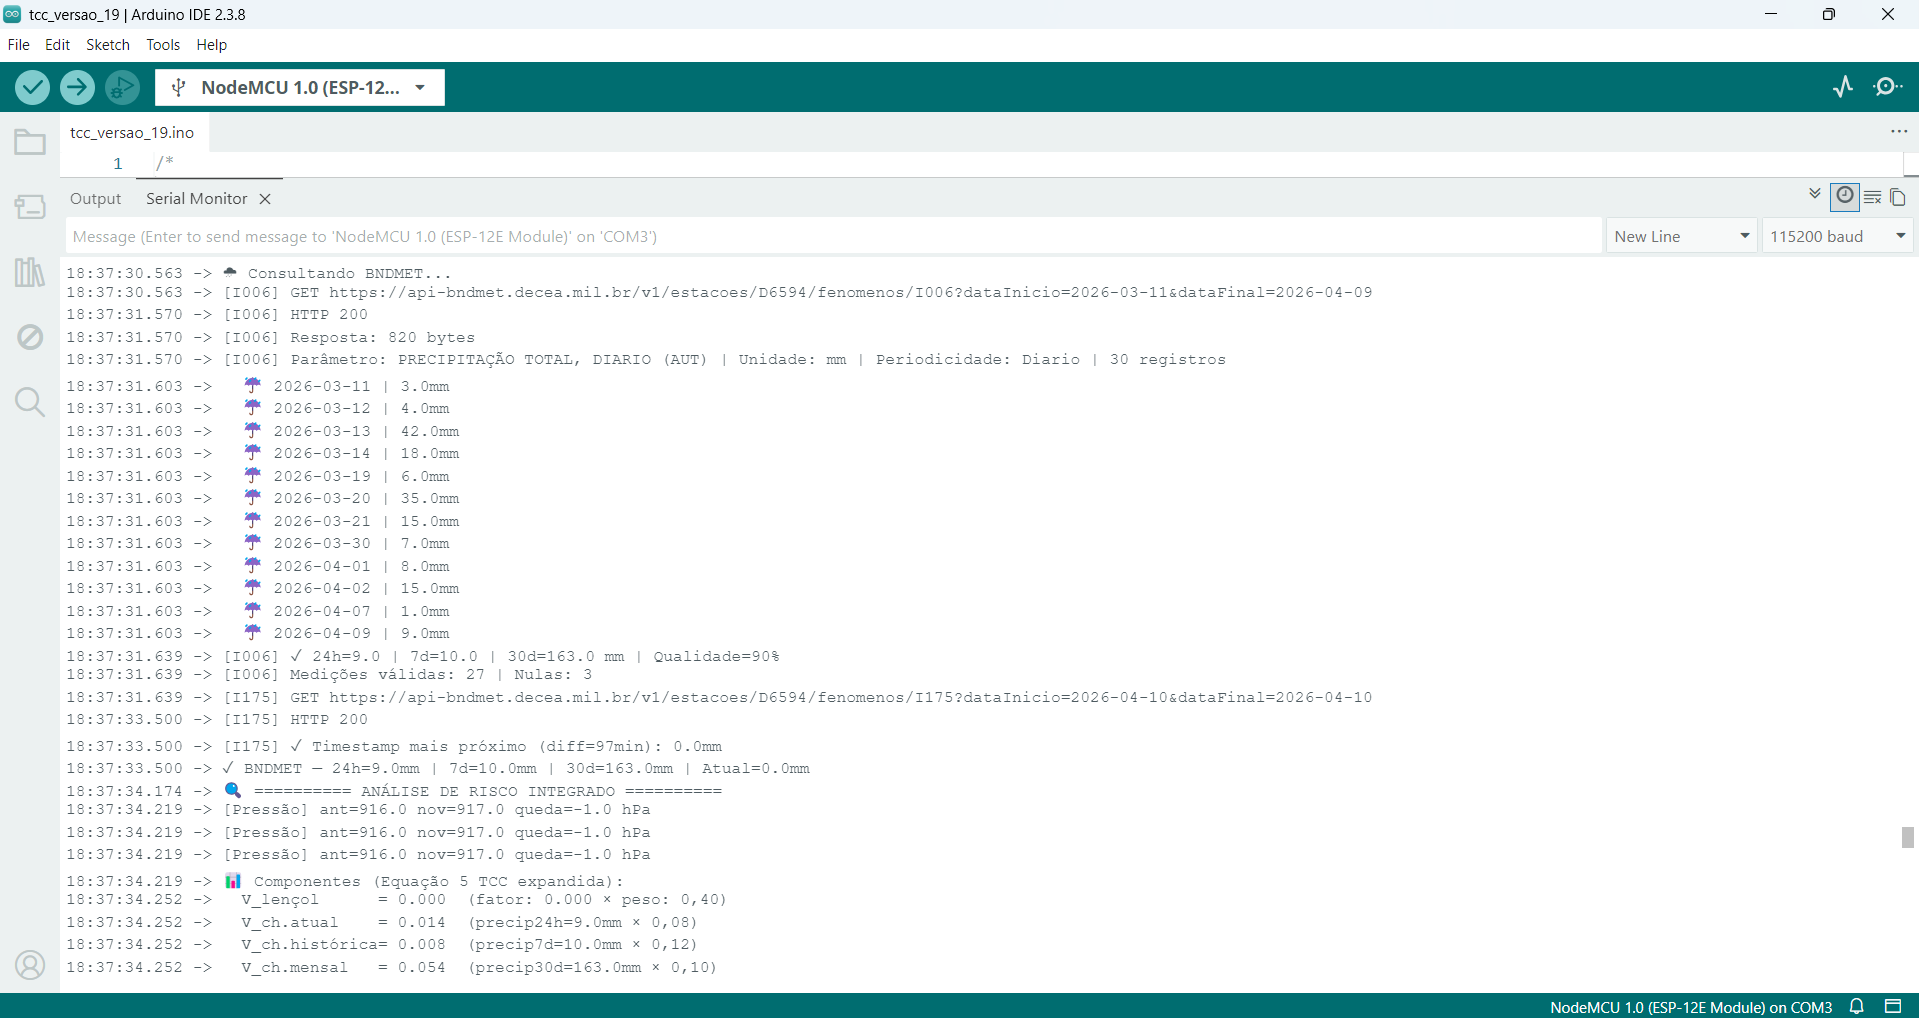
\includegraphics[width=0.85\textwidth]{figures/cap5_serial_bndmet.png}
    \caption{Monitor serial após consulta bem-sucedida à API BNDMET/DECEA:
    acumulados pluviométricos para 24h, 7 dias e 30 dias, precipitação
    horária I175 e índice de qualidade dos dados da estação.}
    \label{fig:serial_bndmet}
    \fonte{Elaborado pela autora.}
\end{figure}

\begin{figure}[htbp]
    \centering
    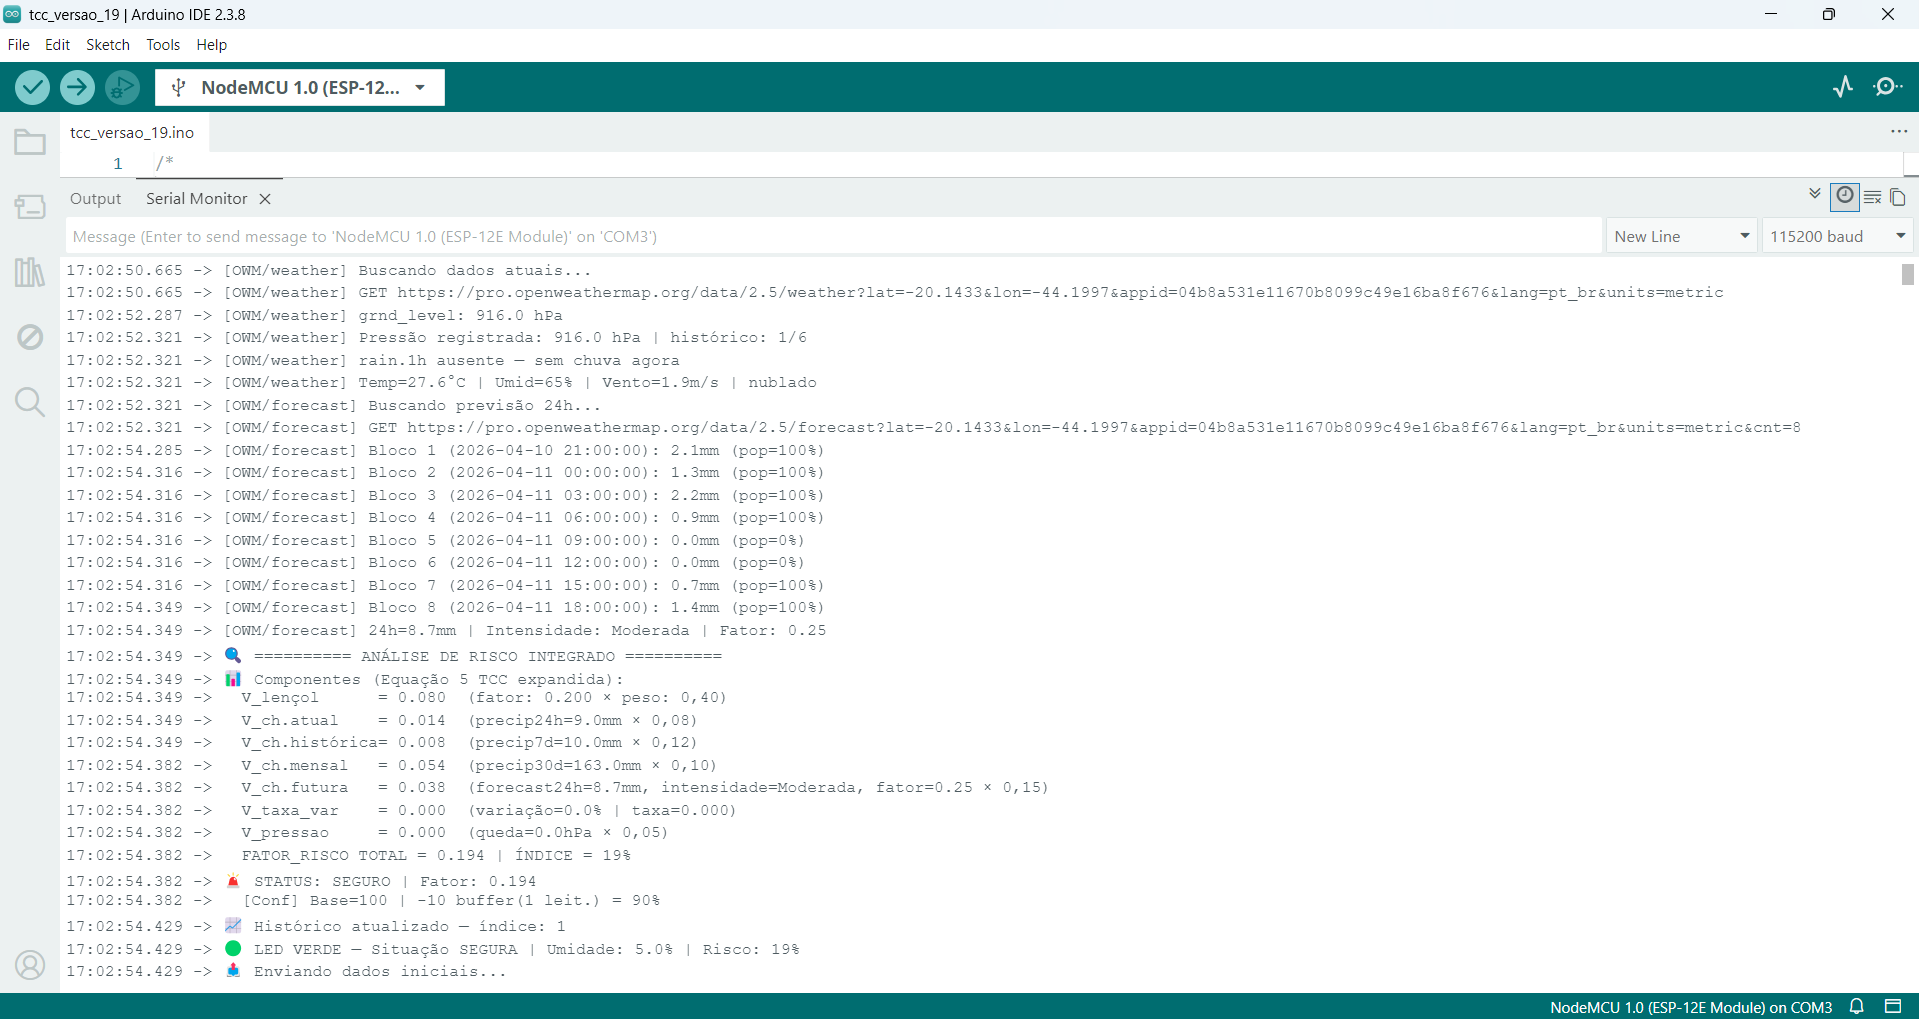
\includegraphics[width=0.95\textwidth]{figures/cap5_serial_owm.png}
    \caption{Monitor serial após consulta à OpenWeatherMap: pressão
    atmosférica, temperatura, chuva atual, acumulado previsto para 24h e
    classificação de intensidade (Fraca / Moderada / Forte / Muito Forte /
    Pancada).}
    \label{fig:serial_owm}
    \fonte{Elaborado pela autora.}
\end{figure}

Com todos os dados coletados, o ciclo de análise calcula os sete
componentes individuais do modelo de risco definido no
\autoref{cap:materiais-metodos} e produz o fator integrado, o nível de alerta, o
índice de confiabilidade e a recomendação operacional. O comando
\texttt{debug} exibe esse painel completo no monitor serial, como
ilustrado nas \autoref{fig:serial_debug_pt1} e
\autoref{fig:serial_debug_pt2}. Quando o mecanismo de
amplificação é ativado --- situação em que o solo apresenta saturação
elevada ao mesmo tempo em que a previsão indica chuva moderada ou
superior ---, o monitor serial registra explicitamente ``Amplificado:
SIM (1,2$\times$)'', conforme demonstra a
\autoref{fig:serial_amplificado}.

\begin{figure}[htbp]
    \centering
    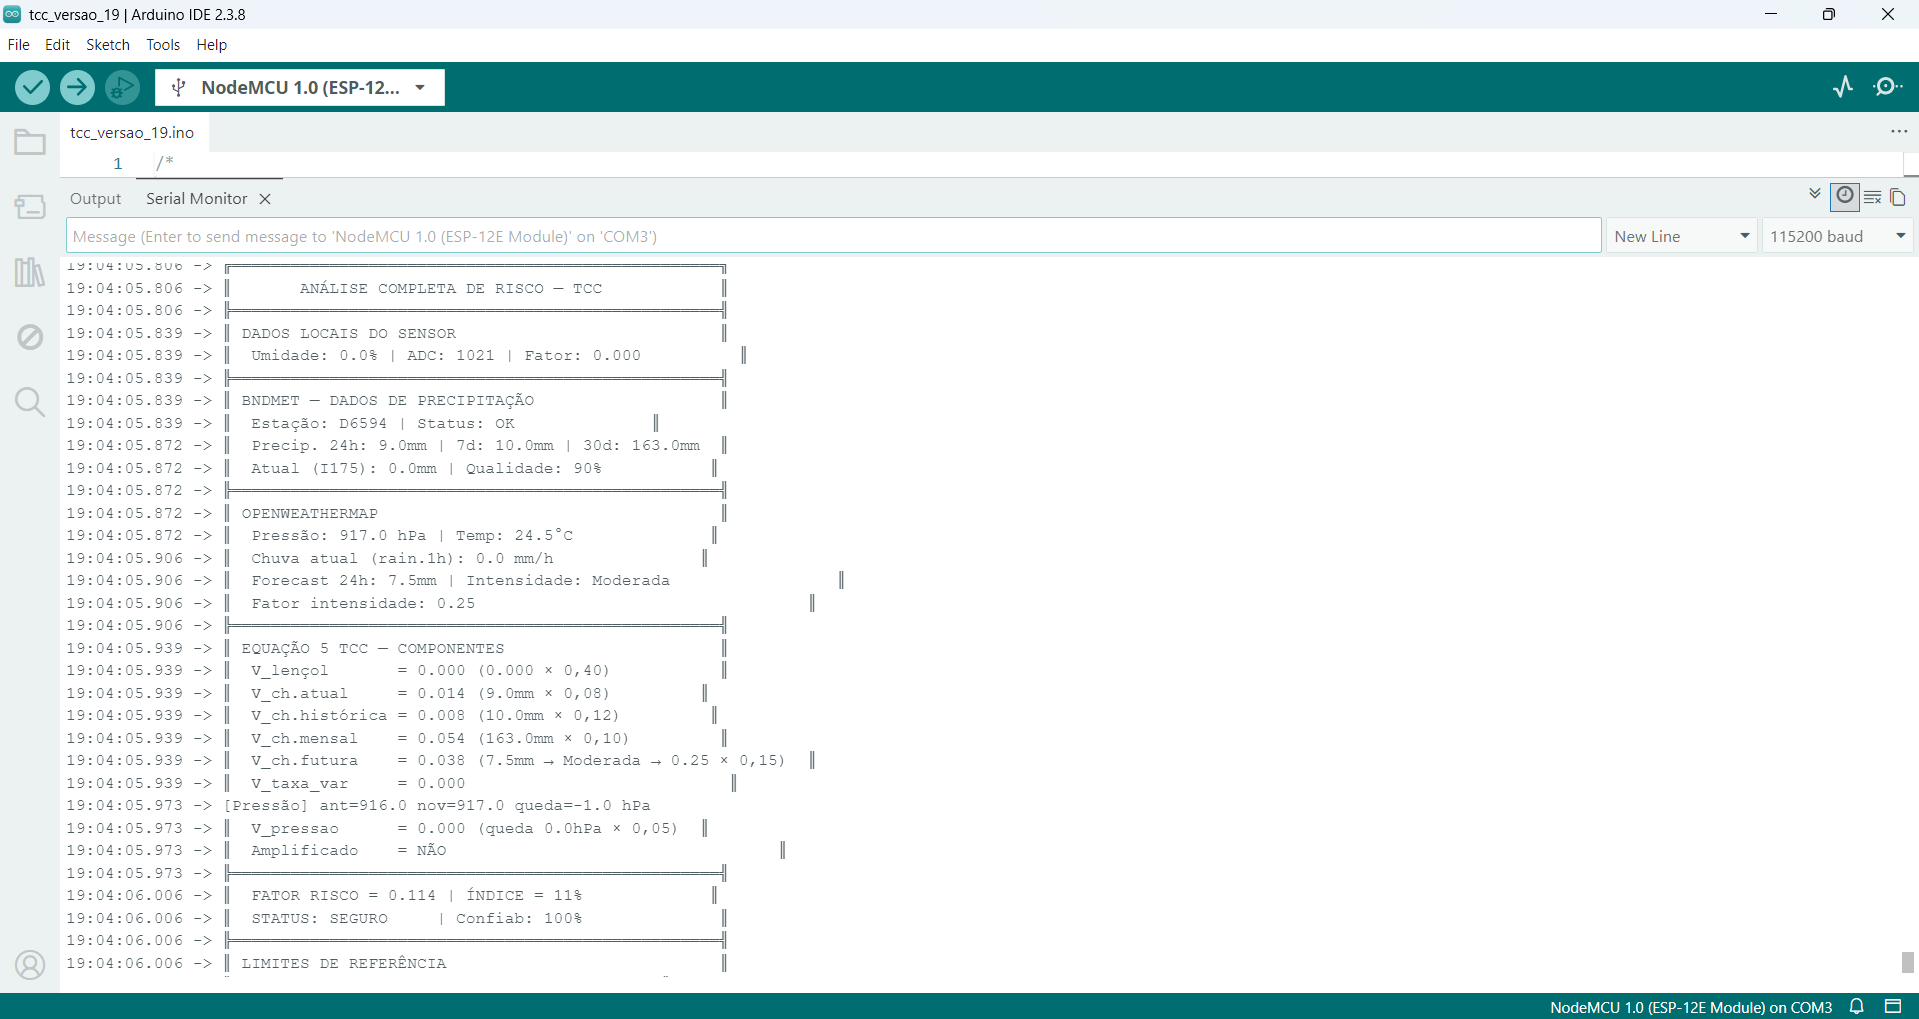
\includegraphics[width=0.85\textwidth]{figures/cap5_serial_debug_pt1.png}
    \caption{Painel de análise de risco exibido pelo comando \texttt{debug}
    (parte~1): os sete componentes individuais do modelo e o fator de risco
    integrado.}
    \label{fig:serial_debug_pt1}
    \fonte{Elaborado pela autora.}
\end{figure}

\begin{figure}[htbp]
    \centering
    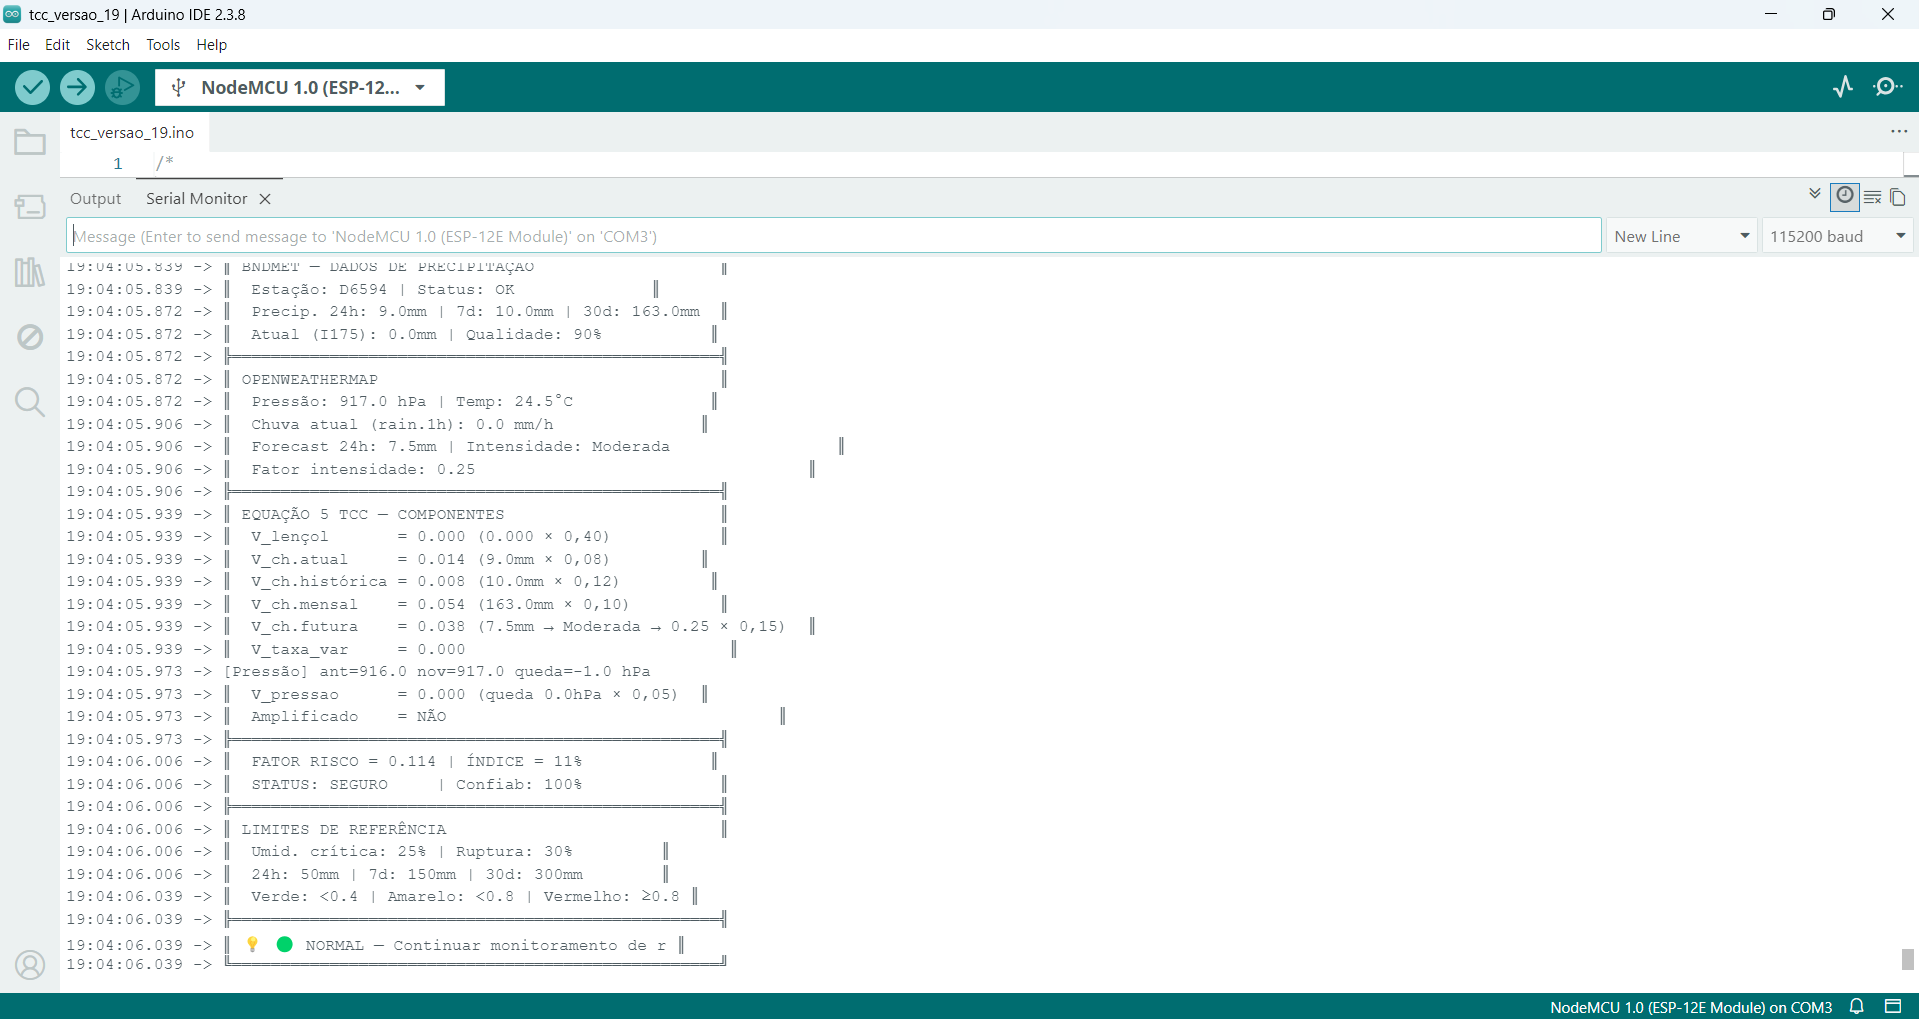
\includegraphics[width=0.85\textwidth]{figures/cap5_serial_debug_pt2.png}
    \caption{Painel de análise de risco exibido pelo comando \texttt{debug}
    (parte~2): nível de alerta, índice de confiabilidade e recomendação
    operacional.}
    \label{fig:serial_debug_pt2}
    \fonte{Elaborado pela autora.}
\end{figure}

\begin{figure}[htbp]
    \centering
    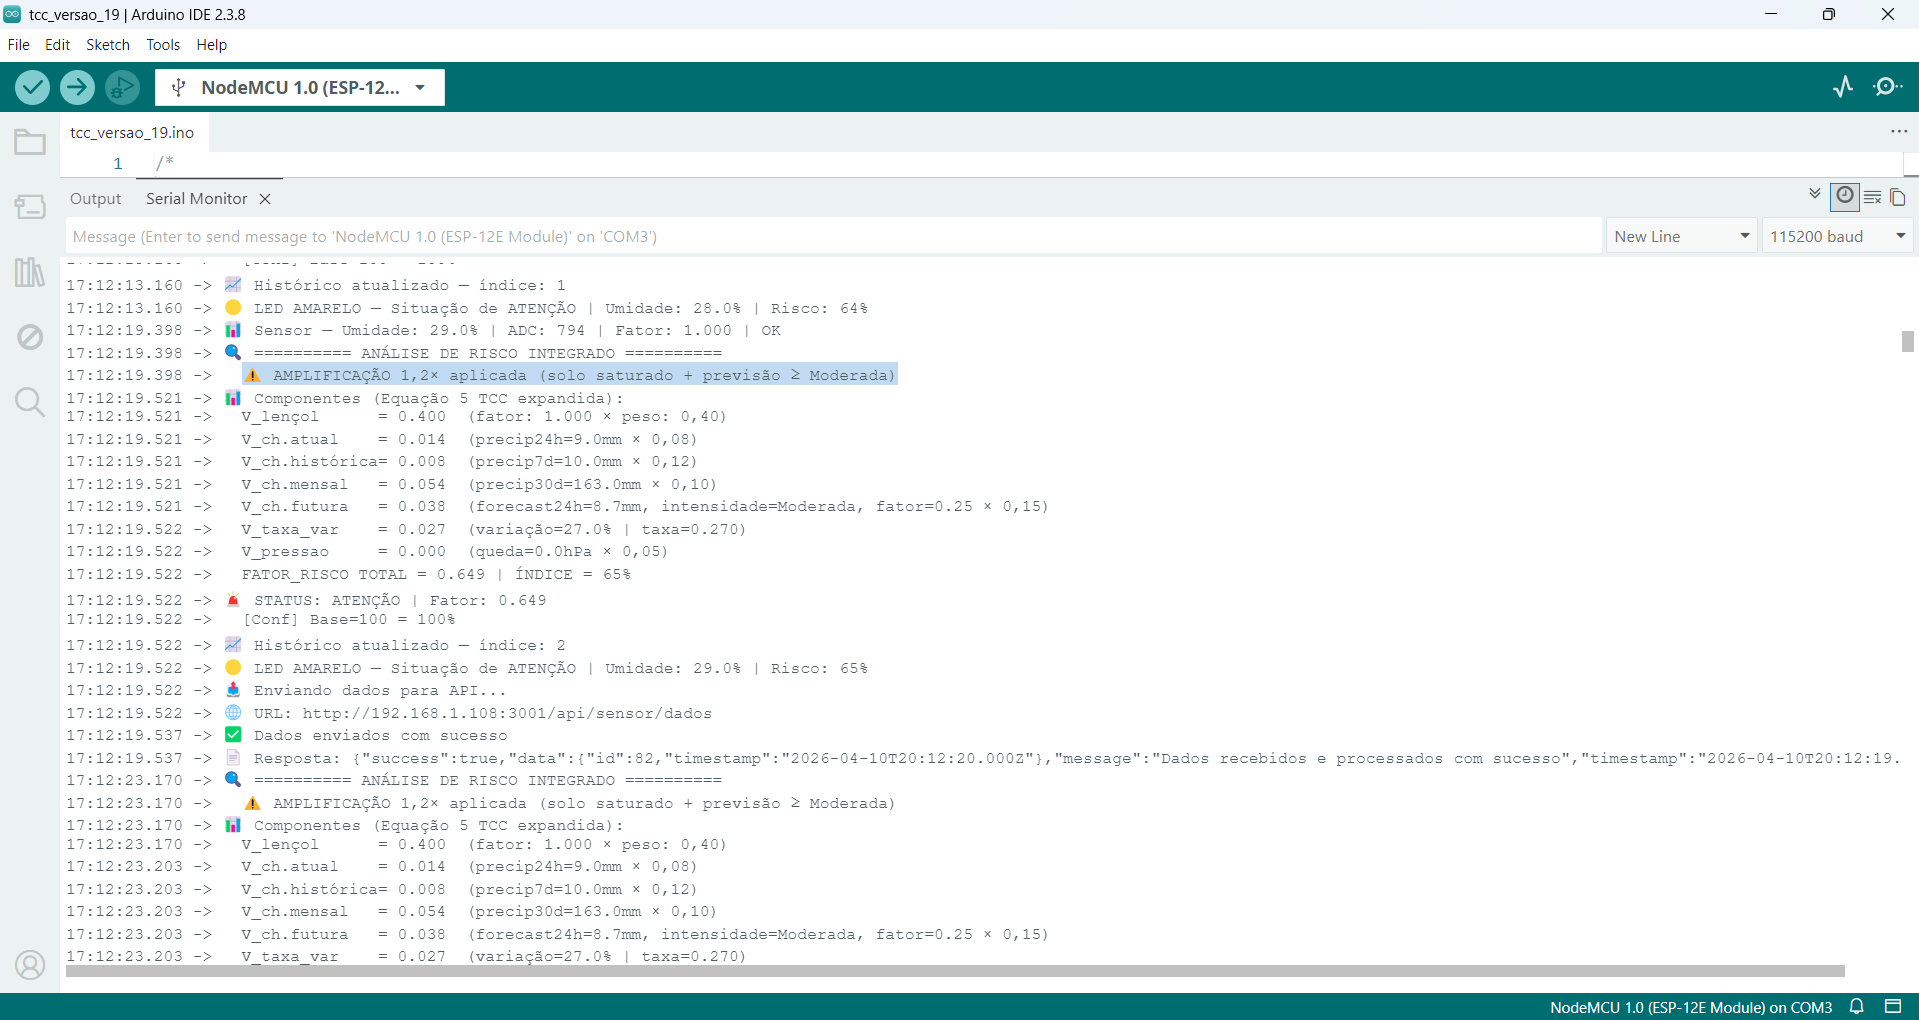
\includegraphics[width=0.85\textwidth]{figures/cap5_serial_amplificado.png}
    \caption{Monitor serial com mecanismo de amplificação $\times 1{,}20$
    ativado: solo em estado avançado de saturação e previsão de chuva
    moderada ou superior satisfeitas simultaneamente.}
    \label{fig:serial_amplificado}
    \fonte{Elaborado pela autora.}
\end{figure}

A recomendação operacional gerada em cada ciclo é composta dinamicamente
pela função \texttt{gerarRecomendacaoDetalhada()}: parte de uma mensagem
base correspondente ao nível de alerta e acrescenta sufixos contextuais
de acordo com o estado atual do sistema. Quando o acumulado de 7 dias
supera 50\,mm, é adicionado ``\texttt{| Solo saturado por chuvas
recentes}''; quando a API BNDMET está indisponível, acrescenta-se
``\texttt{| Dados BNDMET indisponíveis}''; e quando o mecanismo de
amplificação está ativo, inclui-se ``\texttt{| Amplificação de risco
ativa}''. Esses sufixos podem ser combinados, de modo que a recomendação
exibida no \textit{dashboard} e enviada nos alertas por e-mail reflete
com precisão o conjunto de condições vigentes em cada momento.

Quando a API BNDMET retorna erro ou JSON inválido, o sistema exibe
``BNDMET FALHA'' no monitor serial, zera os componentes pluviométricos
históricos e aplica desconto de 25 pontos na confiabilidade da análise.
As tentativas de reconexão passam a ocorrer a cada 30 segundos em vez
do intervalo normal adaptativo, conforme ilustram as
\autoref{fig:serial_bndmet_falha_pt1} e
\autoref{fig:serial_bndmet_falha_pt2}. Se a sincronização NTP ainda não tiver
sido concluída no momento em que a consulta BNDMET seria realizada,
o sistema a adia, exibindo ``NTP ainda não sincronizado --- consulta
BNDMET adiada''. Nesses registros, o campo \texttt{bndmetInicializado}
é serializado como \texttt{false} no \textit{payload} JSON enviado ao
\textit{backend}, que os identifica e os exclui do cálculo da qualidade
média BNDMET exibido no relatório --- evitando que zeros transitórios
dos primeiros ciclos contaminem as estatísticas do período. Dados BNDMET
disponíveis mas com qualidade inferior a 80\% também geram um desconto
adicional de 10 pontos na confiabilidade, porém são utilizados
normalmente no modelo. Se a precipitação horária I175 não registrar
medições para o horário atual, o valor de chuva atual é assumido como
zero, sem prejuízo às demais variáveis.

\begin{figure}[htbp]
    \centering
    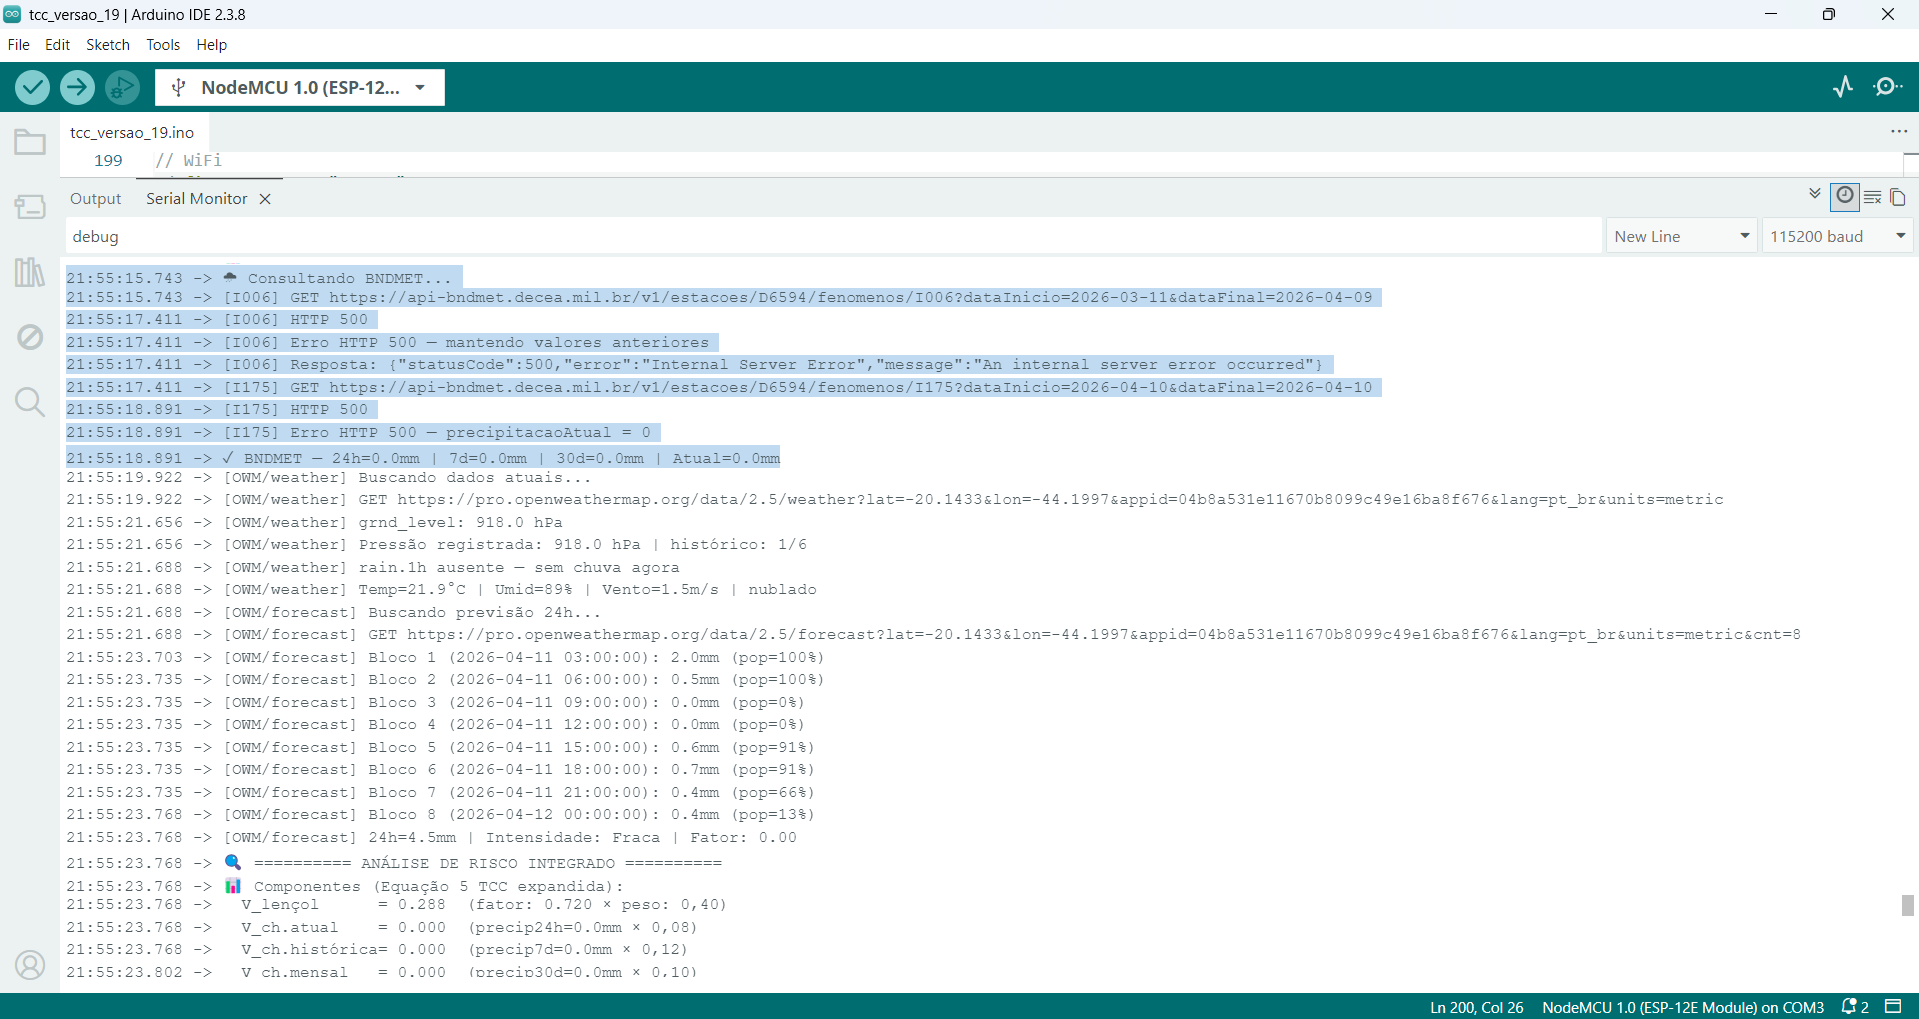
\includegraphics[width=0.85\textwidth]{figures/cap5_serial_bndmet_falha_pt1.png}
    \caption{Monitor serial com falha na API BNDMET/DECEA (parte~1): mensagem ``BNDMET FALHA'' e componentes pluviométricos zerados.}
    \label{fig:serial_bndmet_falha_pt1}
    \fonte{Elaborado pela autora.}
\end{figure}

\begin{figure}[htbp]
    \centering
    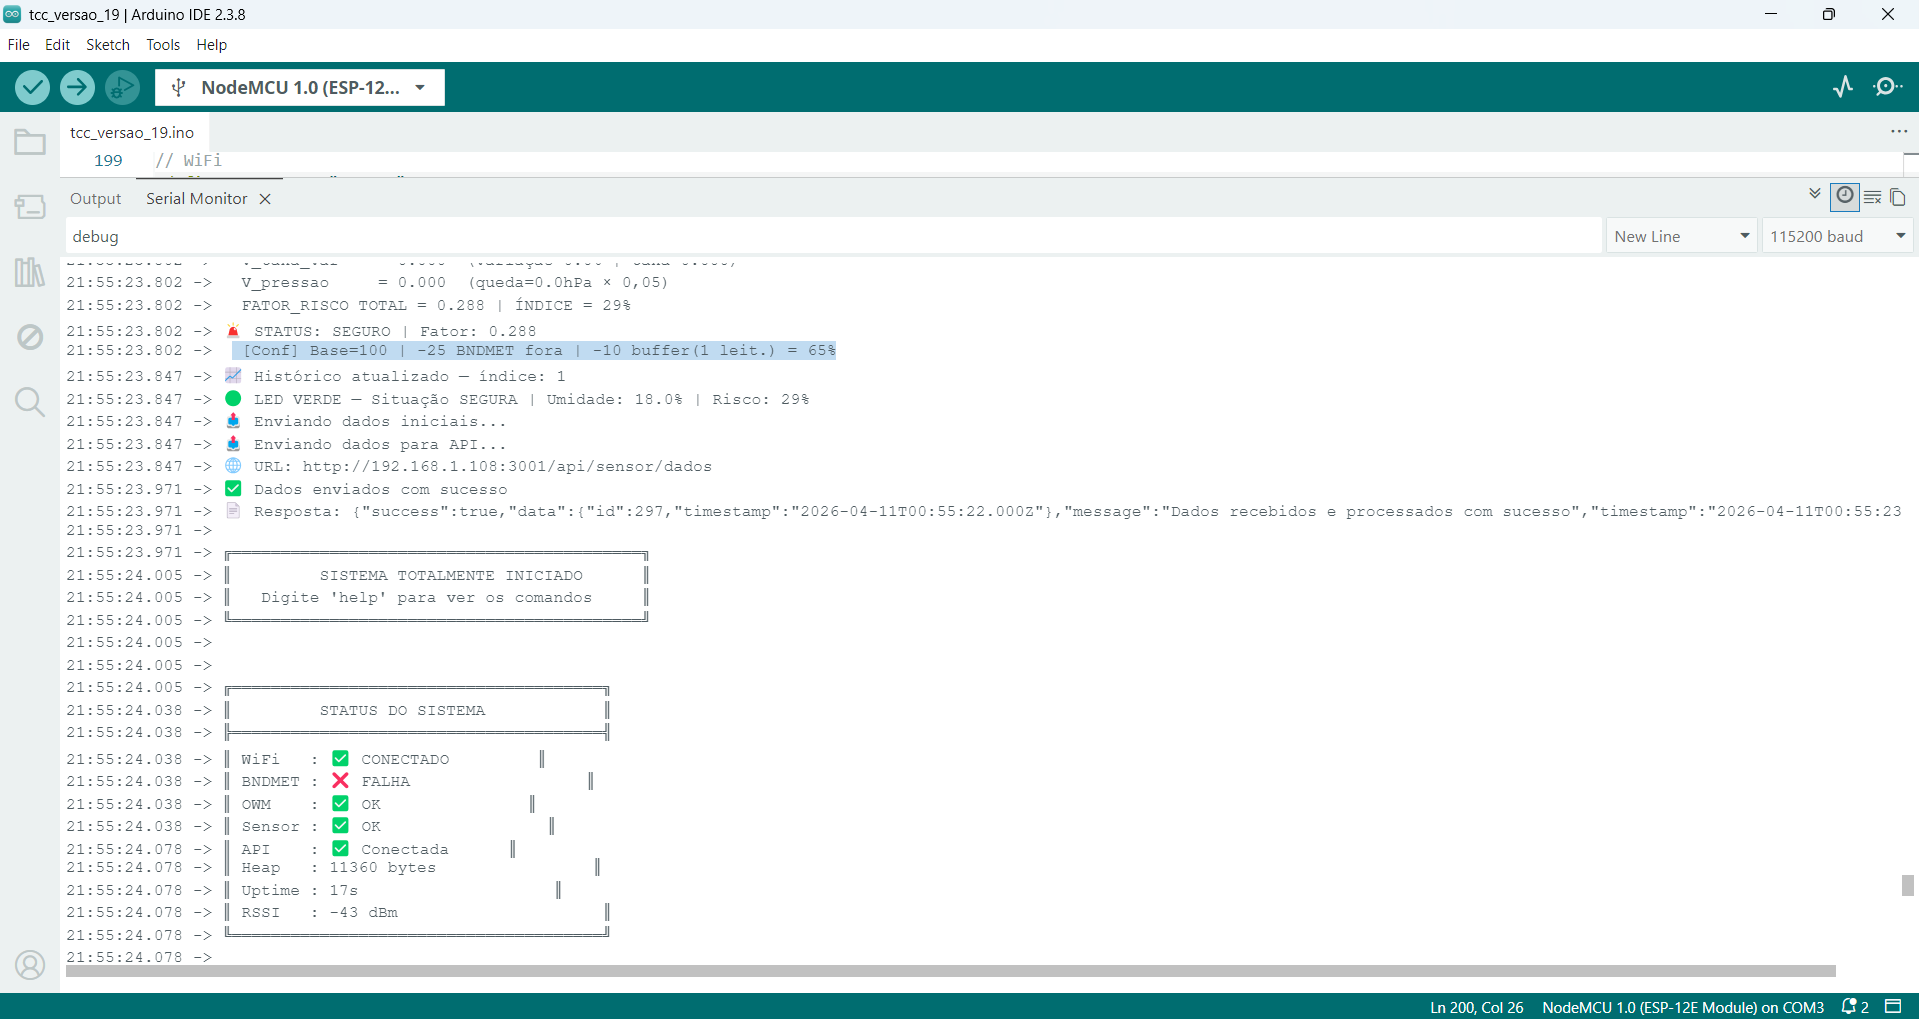
\includegraphics[width=0.85\textwidth]{figures/cap5_serial_bndmet_falha_pt2.png}
    \caption{Monitor serial com falha na API BNDMET/DECEA (parte~2): desconto de 25 pontos registrado na confiabilidade e reconexão acelerada a cada 30 segundos.}
    \label{fig:serial_bndmet_falha_pt2}
    \fonte{Elaborado pela autora.}
\end{figure}

Antes da sincronização NTP ser concluída, o comportamento é distinto da falha de API: o monitor serial exibe a postergação explícita da consulta, como mostra a \autoref{fig:serial_ntp_pendente}.

\begin{figure}[htbp]
    \centering
    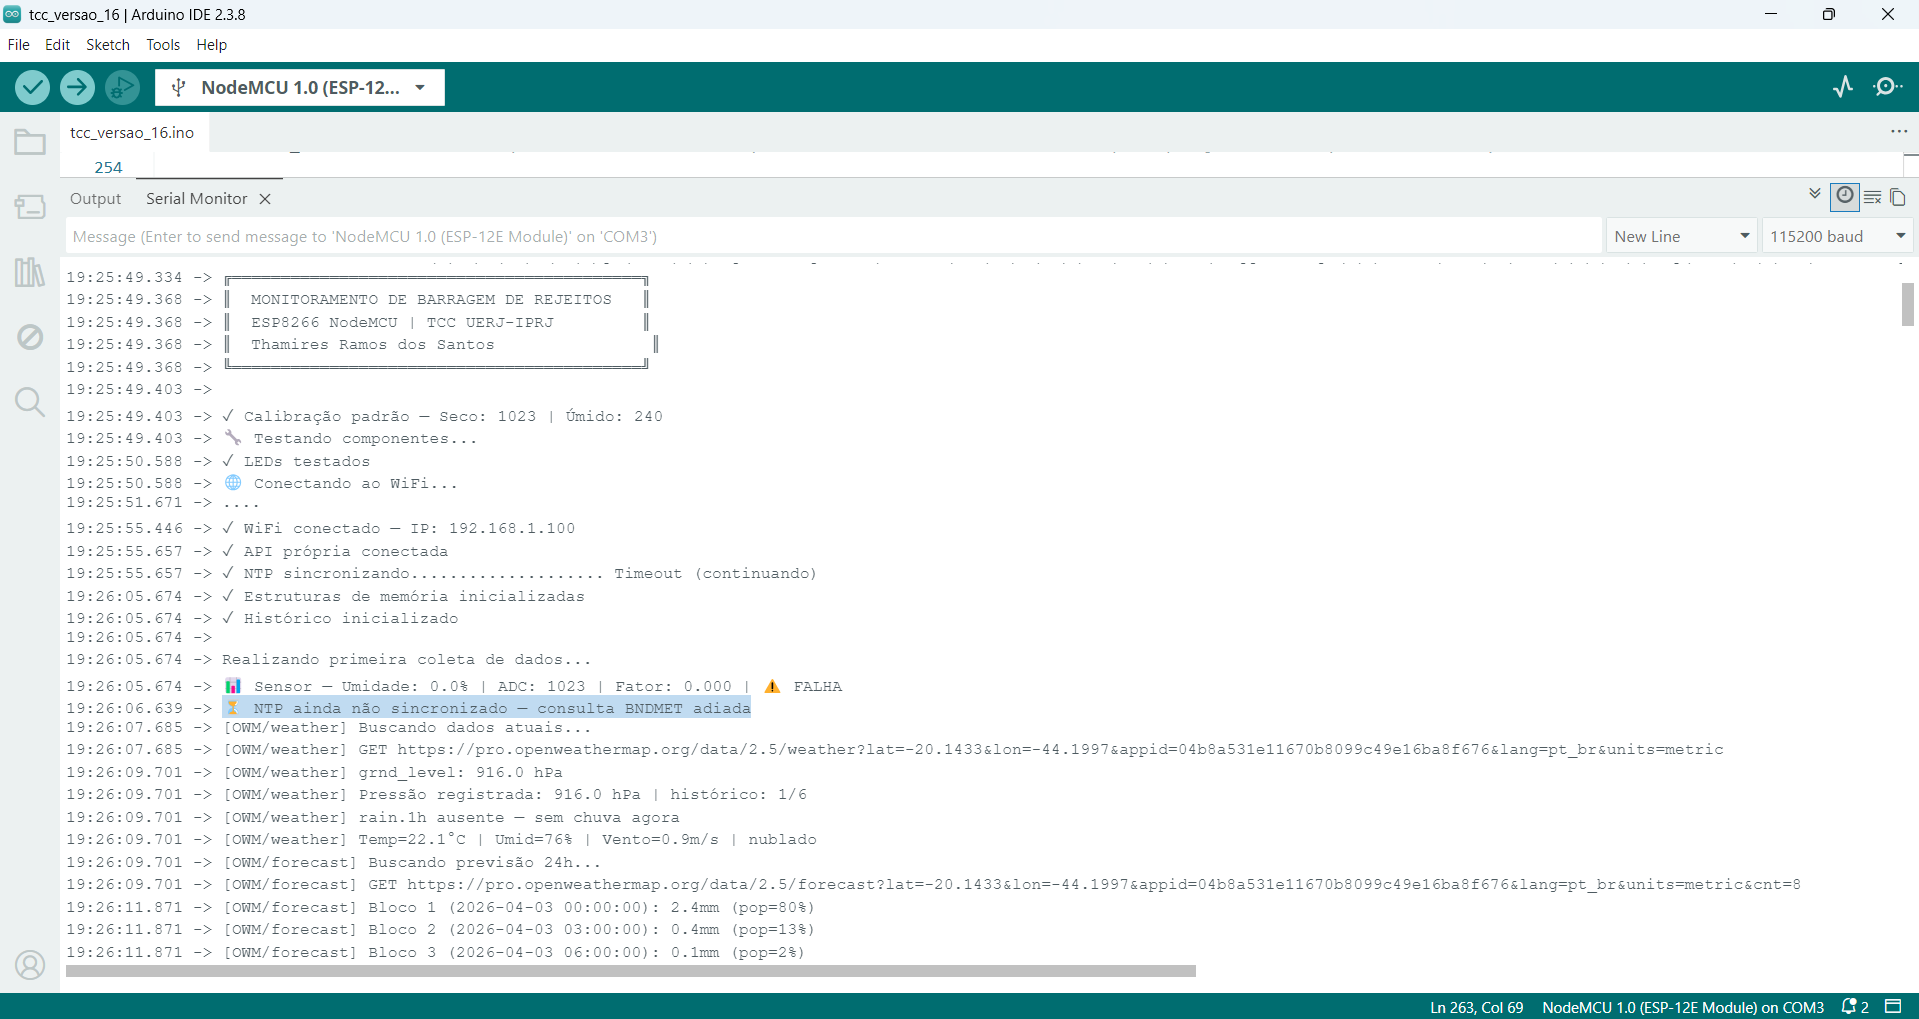
\includegraphics[width=0.85\textwidth]{figures/cap5_serial_ntp_pendente.png}
    \caption{Monitor serial com NTP ainda não sincronizado: mensagem ``NTP ainda não sincronizado --- consulta BNDMET adiada'' e consulta postergada para o próximo ciclo, sem penalidade de indisponibilidade de API.}
    \label{fig:serial_ntp_pendente}
    \fonte{Elaborado pela autora.}
\end{figure}

Quando os dados BNDMET estão disponíveis mas a estação registra muitas medições nulas, o índice de qualidade fica abaixo de 80\% e um desconto adicional é aplicado, conforme ilustram as \autoref{fig:serial_bndmet_qualidade_baixa_pt1} e \autoref{fig:serial_bndmet_qualidade_baixa_pt2}. Esta condição não ocorreu espontaneamente durante os testes em tempo real; para viabilizar a captura, a data da consulta foi ajustada para um intervalo histórico real da estação D6594 em que o número de medições nulas foi elevado, validando o comportamento do sistema sem reproduzir a situação em operação contínua.

\begin{figure}[htbp]
    \centering
    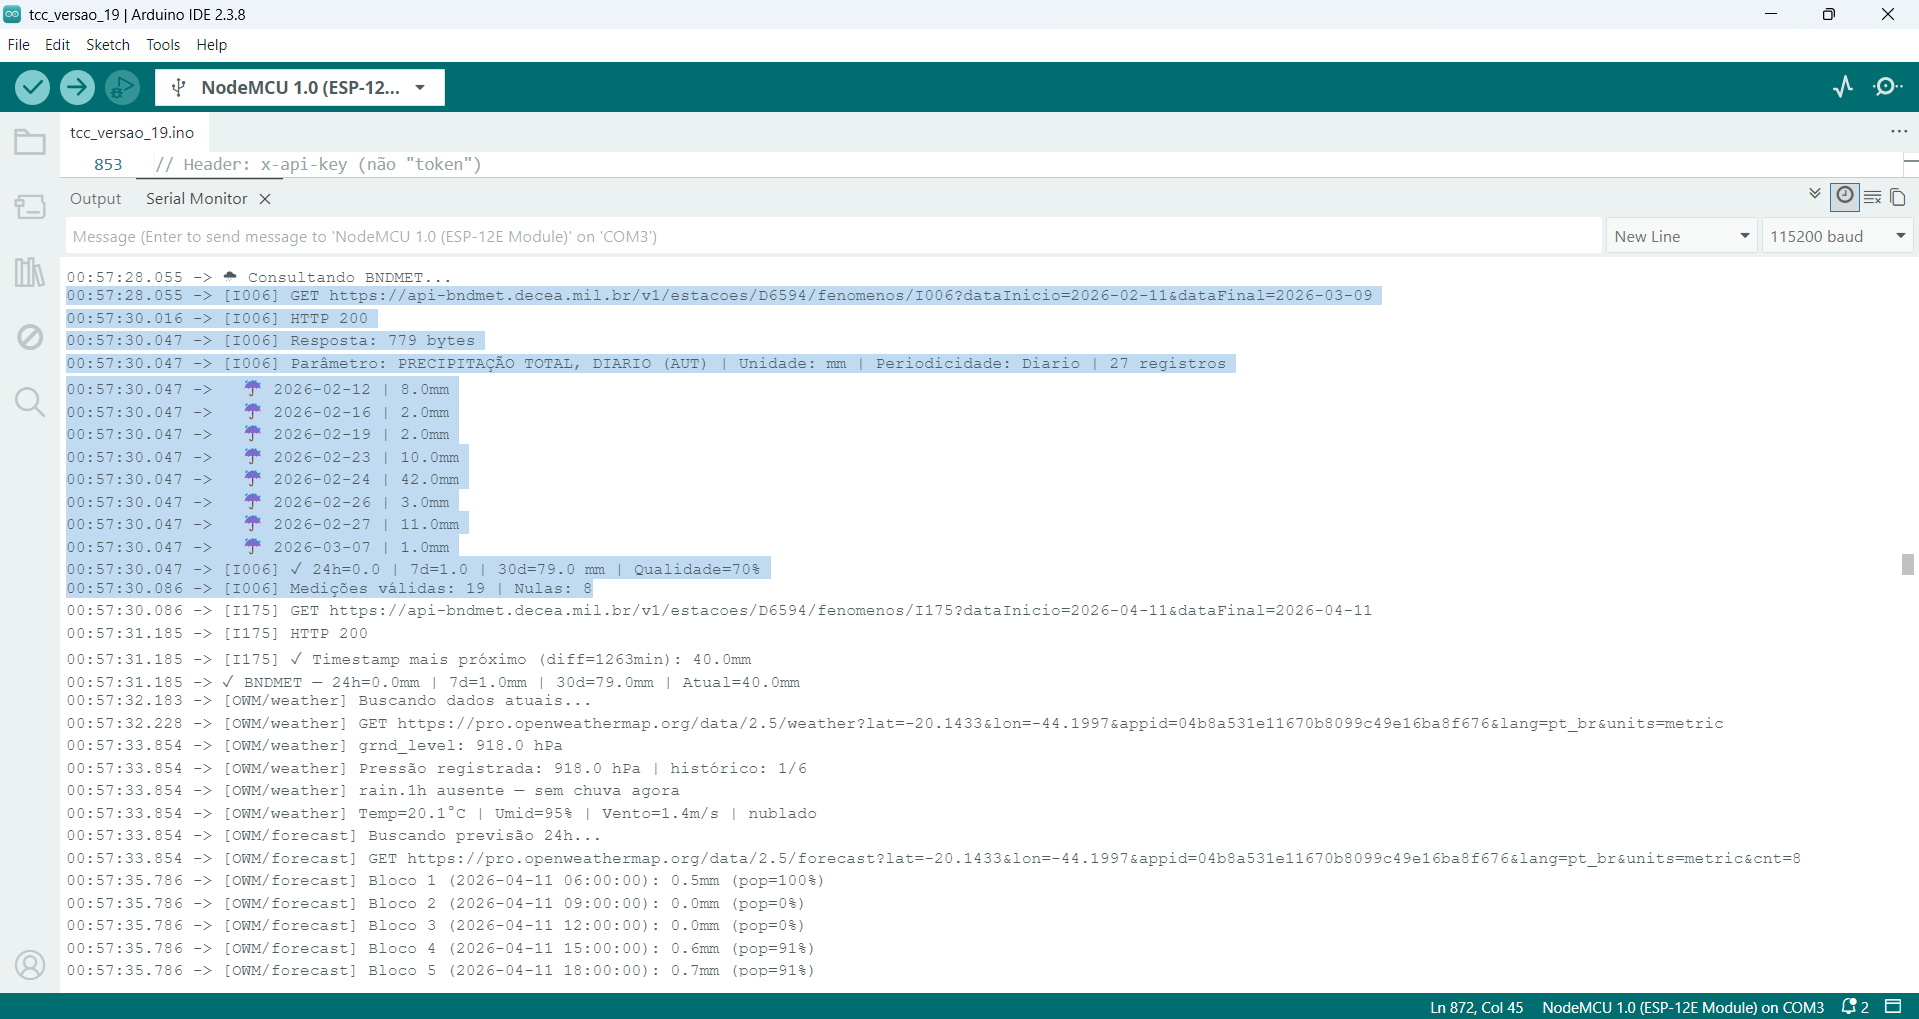
\includegraphics[width=0.85\textwidth]{figures/cap5_serial_bndmet_qualidade_baixa_pt1.png}
    \caption{Monitor serial com dados BNDMET disponíveis mas índice de qualidade inferior a 80\% (parte~1): qualidade dos dados registrada abaixo do limiar aceitável.}
    \label{fig:serial_bndmet_qualidade_baixa_pt1}
    \fonte{Elaborado pela autora.}
\end{figure}

\begin{figure}[htbp]
    \centering
    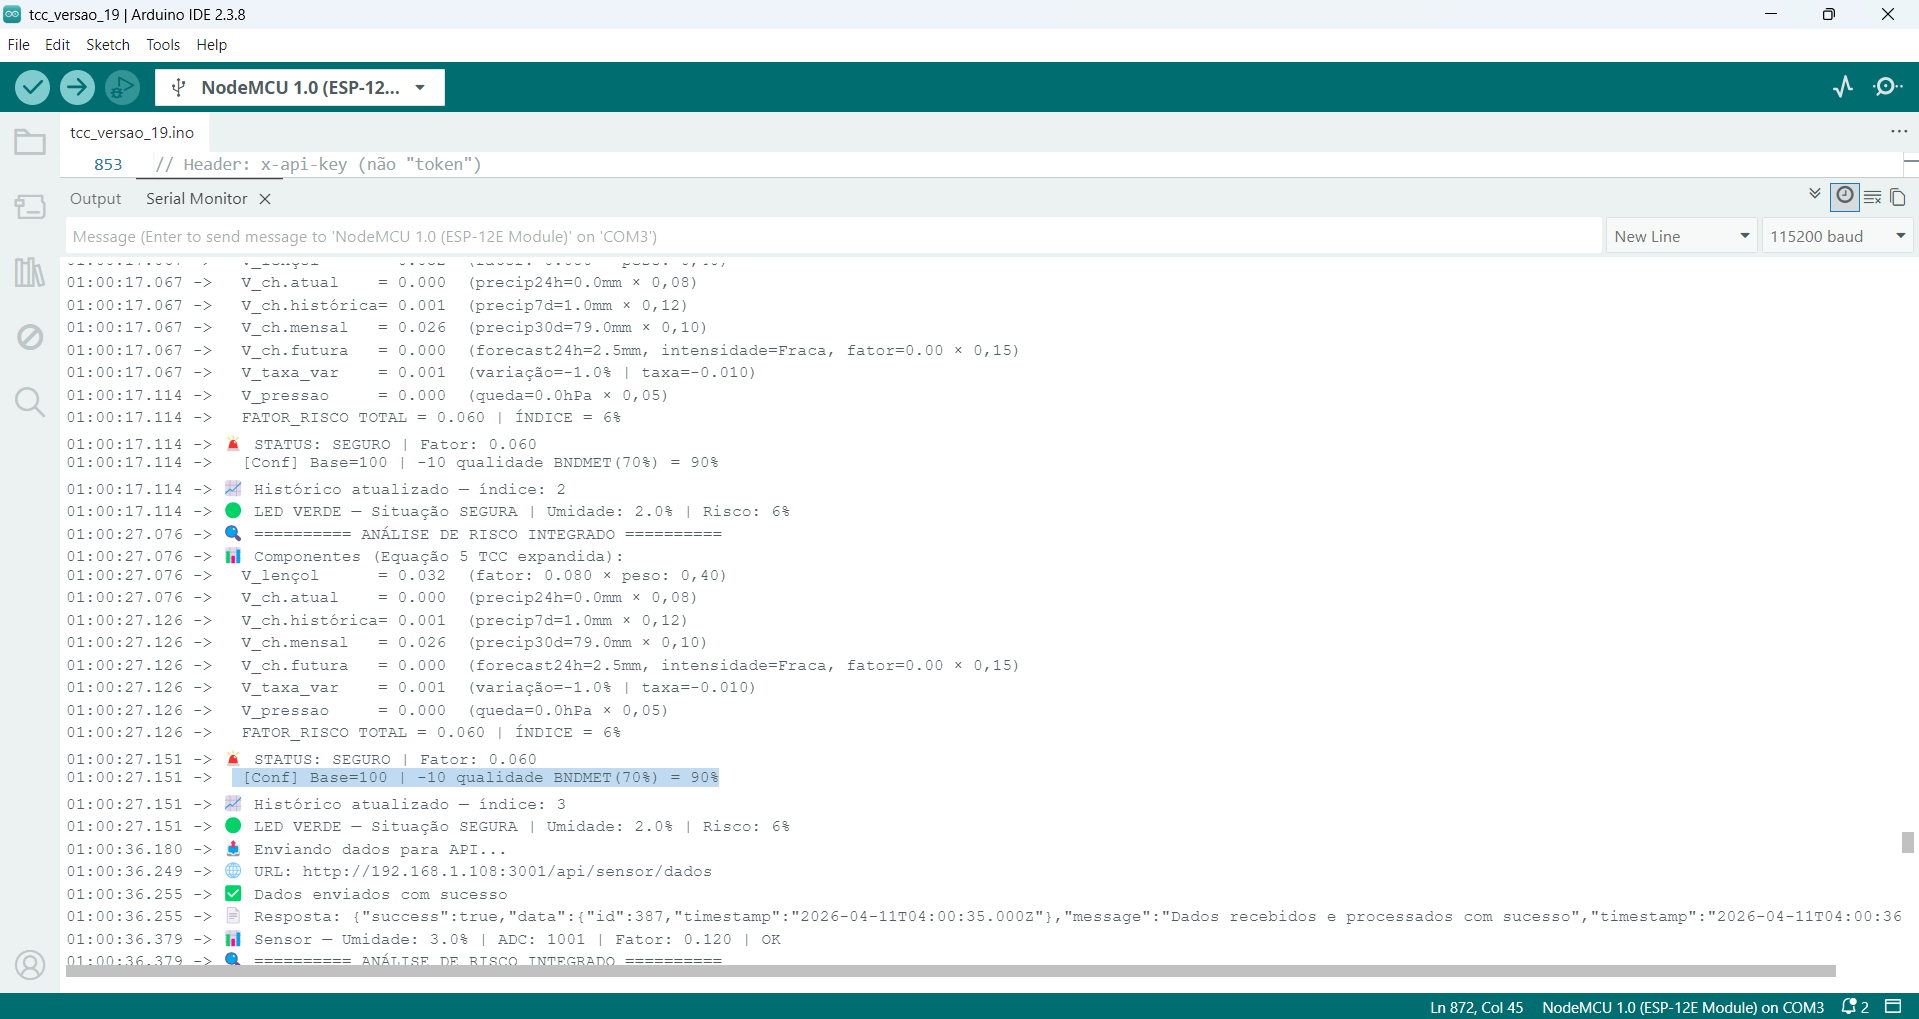
\includegraphics[width=0.85\textwidth]{figures/cap5_serial_bndmet_qualidade_baixa_pt2.png}
    \caption{Monitor serial com dados BNDMET disponíveis mas índice de qualidade inferior a 80\% (parte~2): desconto adicional de 10 pontos registrado na confiabilidade; precipitações utilizadas normalmente no modelo de risco.}
    \label{fig:serial_bndmet_qualidade_baixa_pt2}
    \fonte{Elaborado pela autora.}
\end{figure}

A ausência de medições horárias I175 para o momento da consulta é tratada de forma silenciosa, como demonstram as \autoref{fig:serial_i175_sem_medicao_pt1} e \autoref{fig:serial_i175_sem_medicao_pt2}: o sistema assume precipitação atual zero sem interromper o ciclo. Esta condição foi observada em período noturno durante os testes, sendo um evento de ocorrência irregular que não pôde ser reproduzido de forma controlada.

\begin{figure}[htbp]
    \centering
    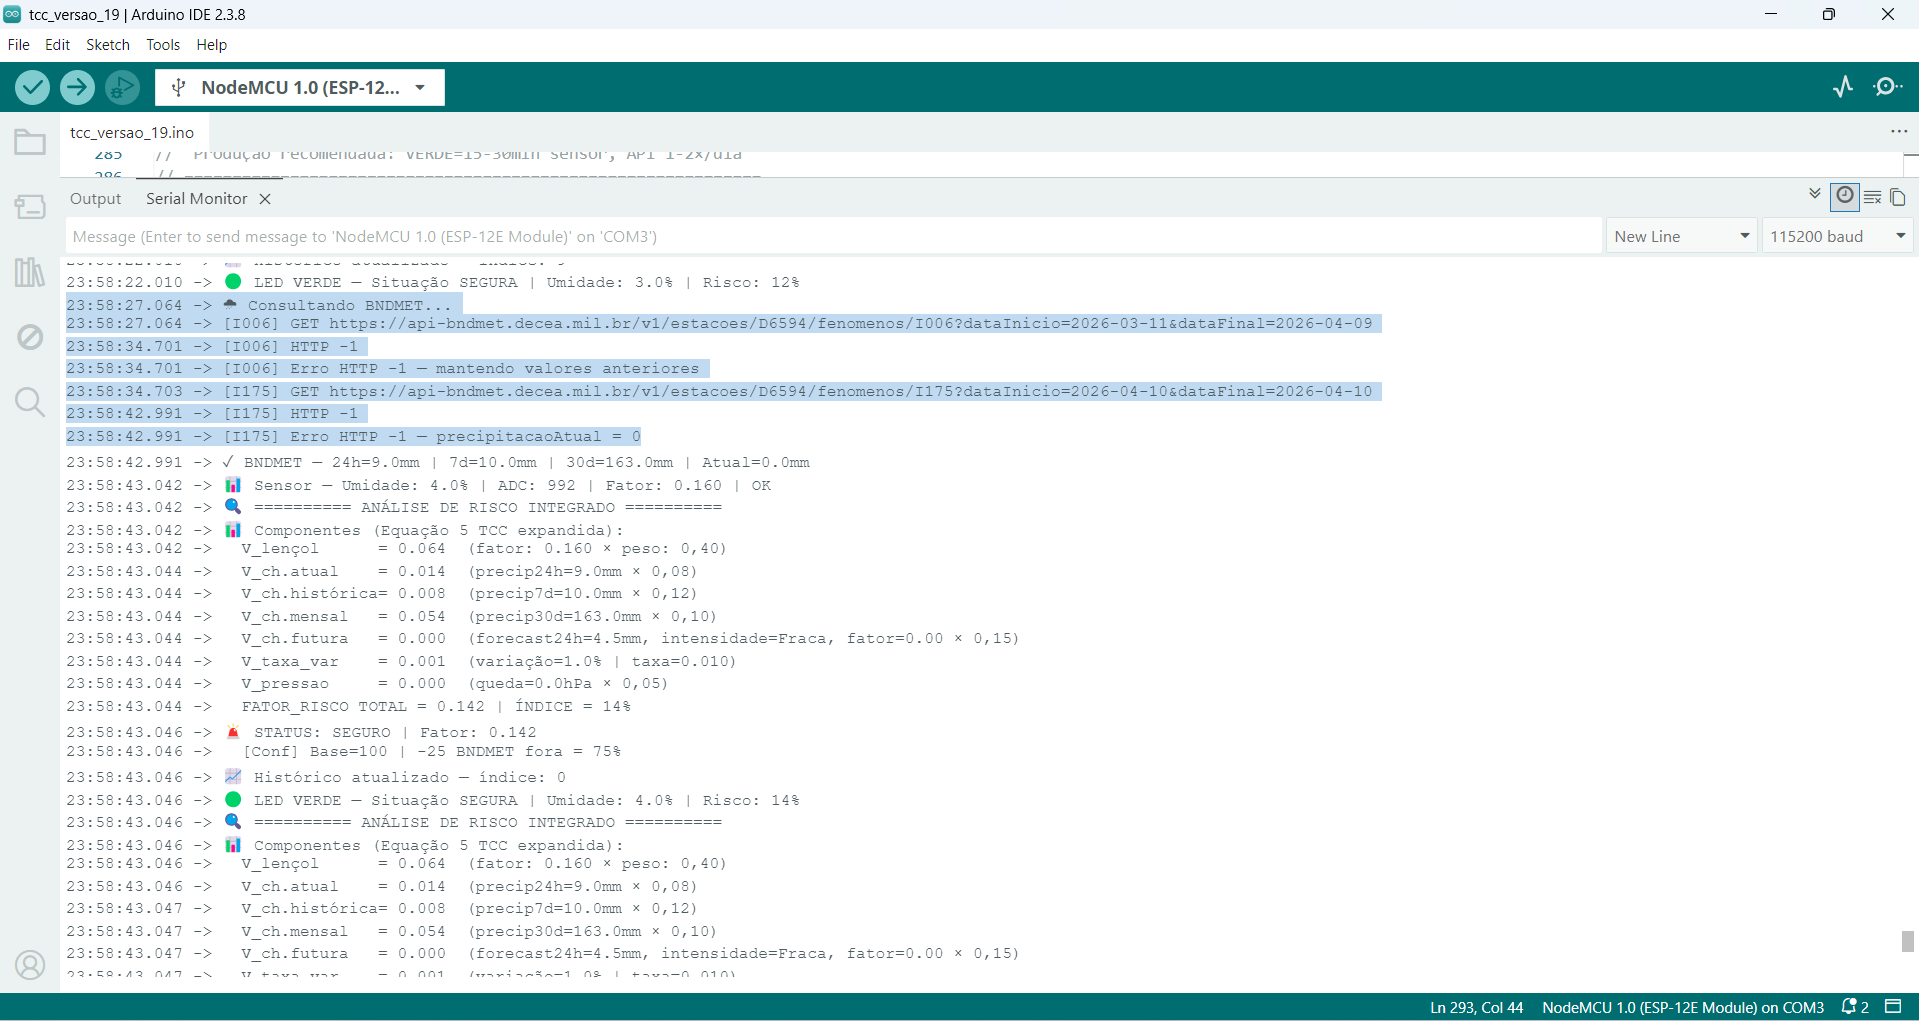
\includegraphics[width=0.85\textwidth]{figures/cap5_serial_i175_sem_medicao_pt1.png}
    \caption{Monitor serial com fenômeno I175 sem medições para o horário atual (parte~1): ausência de dados horários identificada pelo sistema.}
    \label{fig:serial_i175_sem_medicao_pt1}
    \fonte{Elaborado pela autora.}
\end{figure}

\begin{figure}[htbp]
    \centering
    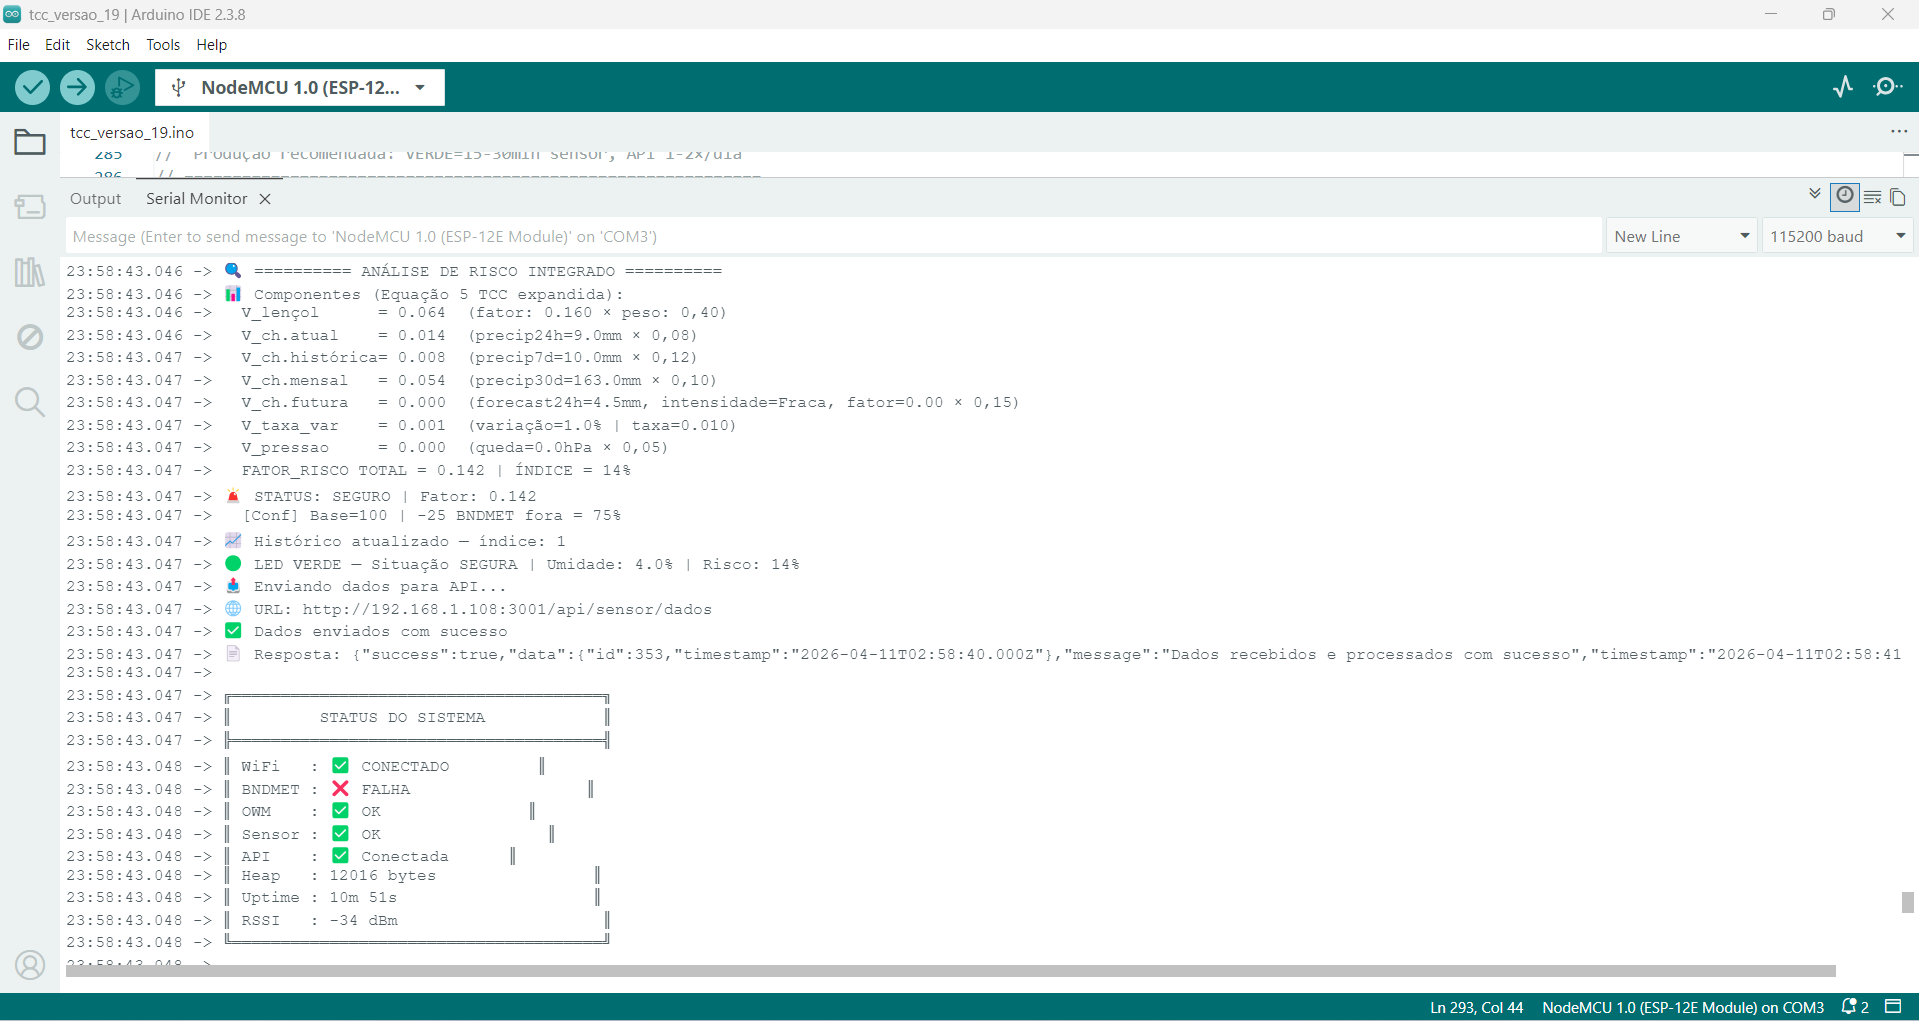
\includegraphics[width=0.85\textwidth]{figures/cap5_serial_i175_sem_medicao_pt2.png}
    \caption{Monitor serial com fenômeno I175 sem medições para o horário atual (parte~2): precipitação horária assumida como zero e demais variáveis do modelo calculadas normalmente.}
    \label{fig:serial_i175_sem_medicao_pt2}
    \fonte{Elaborado pela autora.}
\end{figure}

A OpenWeatherMap segue comportamento simétrico: quando indisponível, os
componentes de previsão e pressão atmosférica são zerados e a
confiabilidade perde 15 pontos, com \textit{retry} acelerado a cada 30
segundos, conforme ilustram as \autoref{fig:serial_owm_falha_pt1} e \autoref{fig:serial_owm_falha_pt2}.

\begin{figure}[htbp]
    \centering
    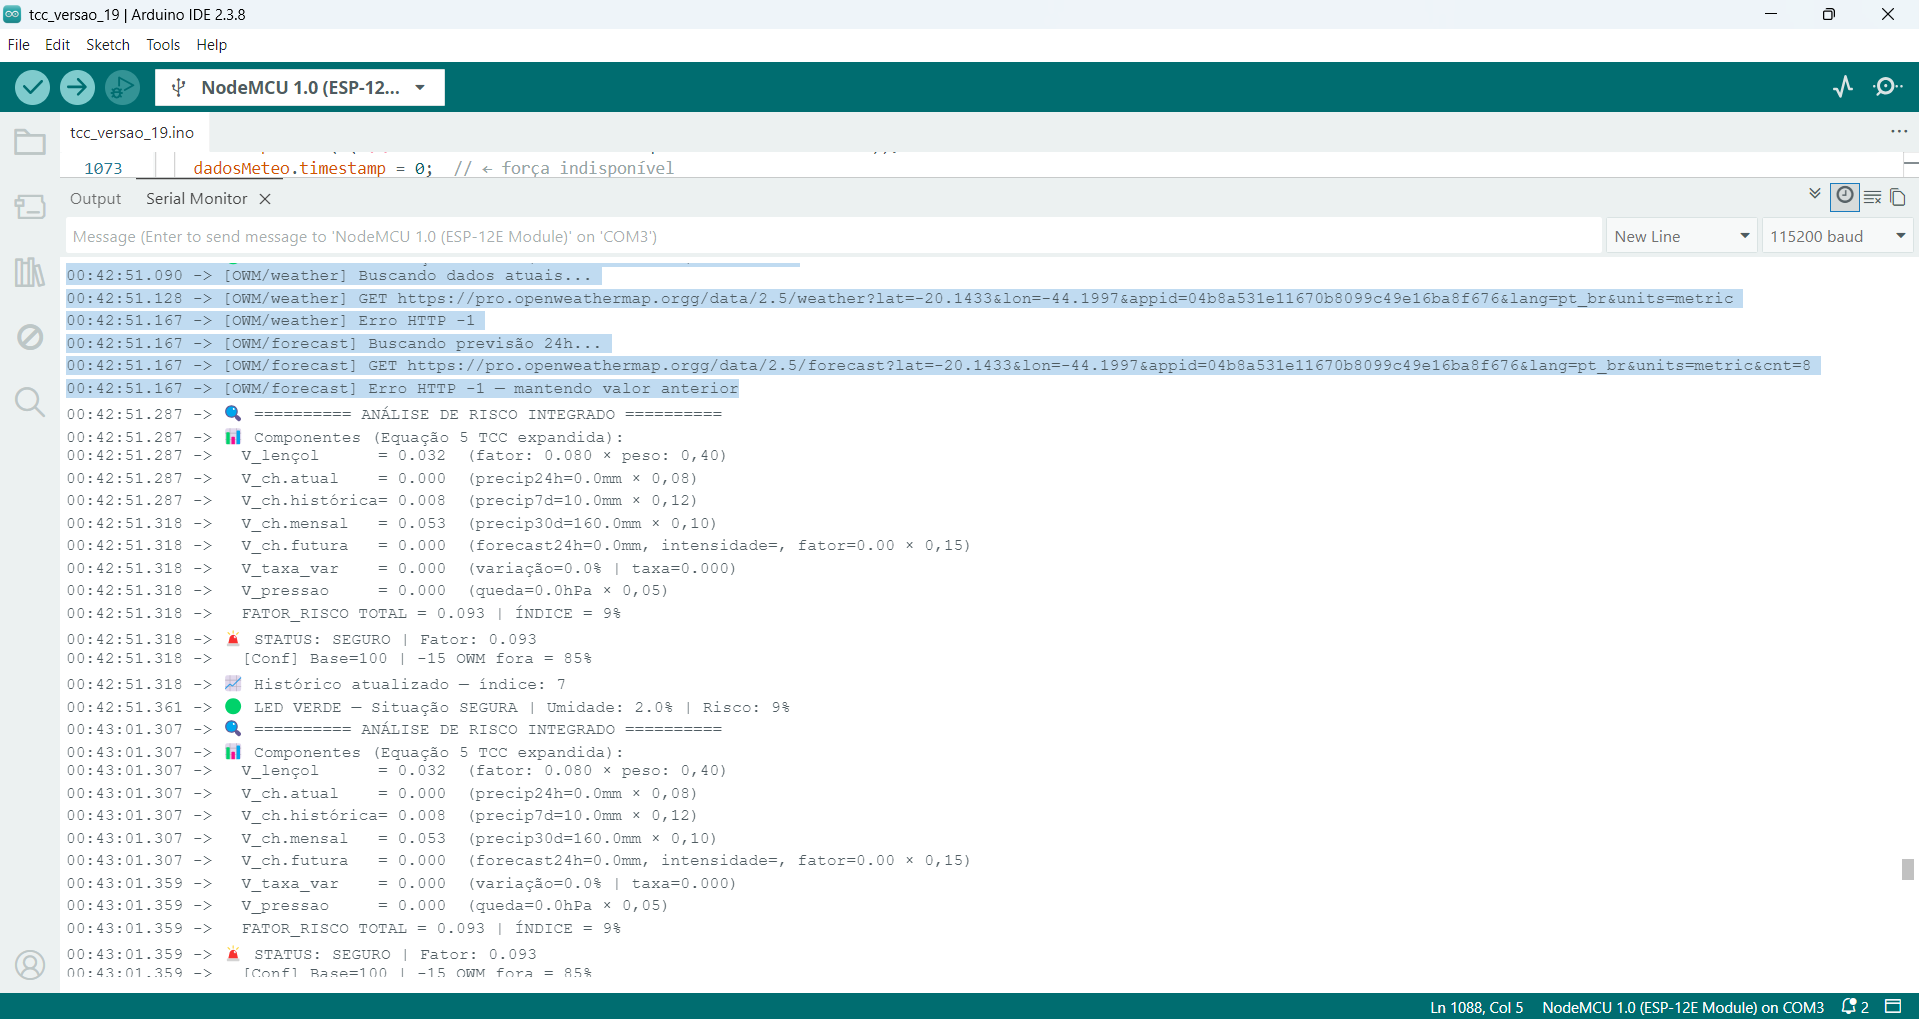
\includegraphics[width=0.85\textwidth]{figures/cap5_serial_owm_falha_pt1.png}
    \caption{Monitor serial com OpenWeatherMap indisponível (parte~1): componentes de previsão e pressão zerados.}
    \label{fig:serial_owm_falha_pt1}
    \fonte{Elaborado pela autora.}
\end{figure}

\begin{figure}[htbp]
    \centering
    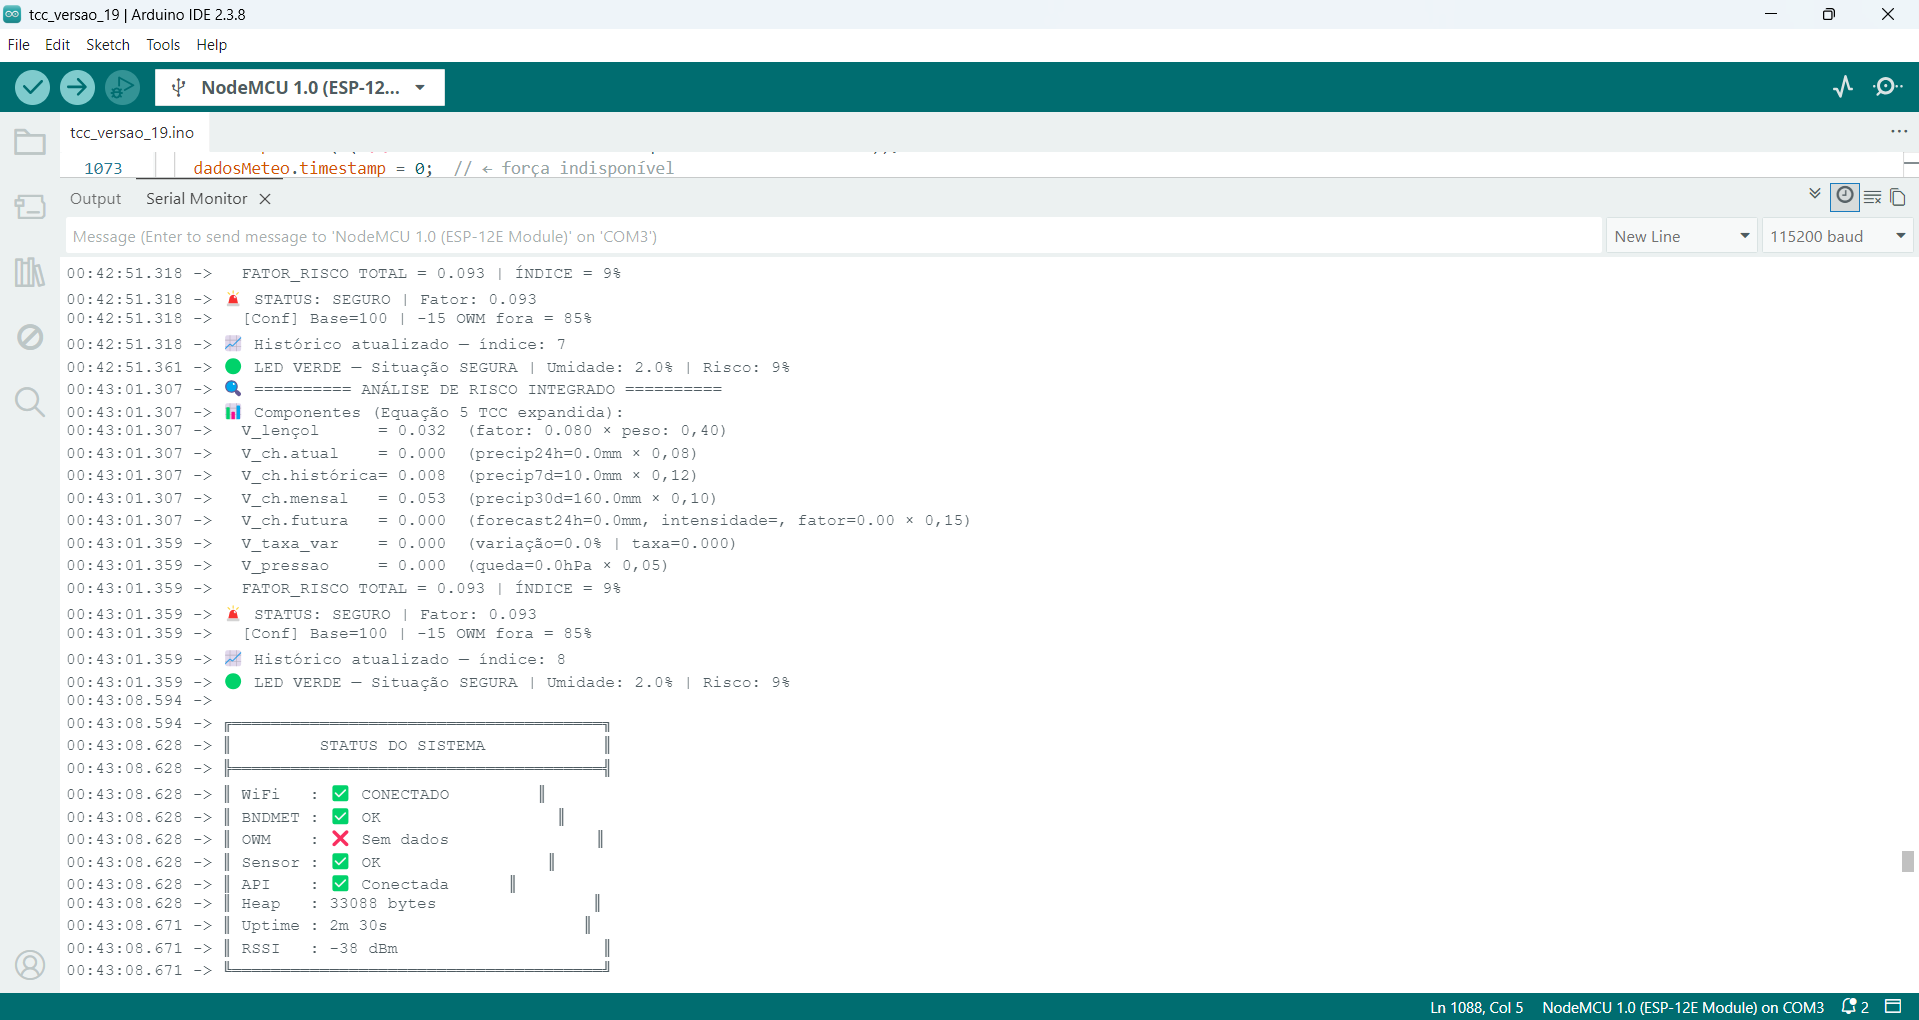
\includegraphics[width=0.85\textwidth]{figures/cap5_serial_owm_falha_pt2.png}
    \caption{Monitor serial com OpenWeatherMap indisponível (parte~2): desconto de 15 pontos na confiabilidade e \textit{retry} acelerado ativado para a próxima tentativa.}
    \label{fig:serial_owm_falha_pt2}
    \fonte{Elaborado pela autora.}
\end{figure}

Durante o estado de ruptura ativa, a confiabilidade é fixada em 100\% independentemente de qualquer fonte indisponível, pois o hardware confirma o estado diretamente, conforme demonstram as \autoref{fig:serial_ruptura_confiabilidade_100_pt1} e \autoref{fig:serial_ruptura_confiabilidade_100_pt2}.

\begin{figure}[htbp]
    \centering
    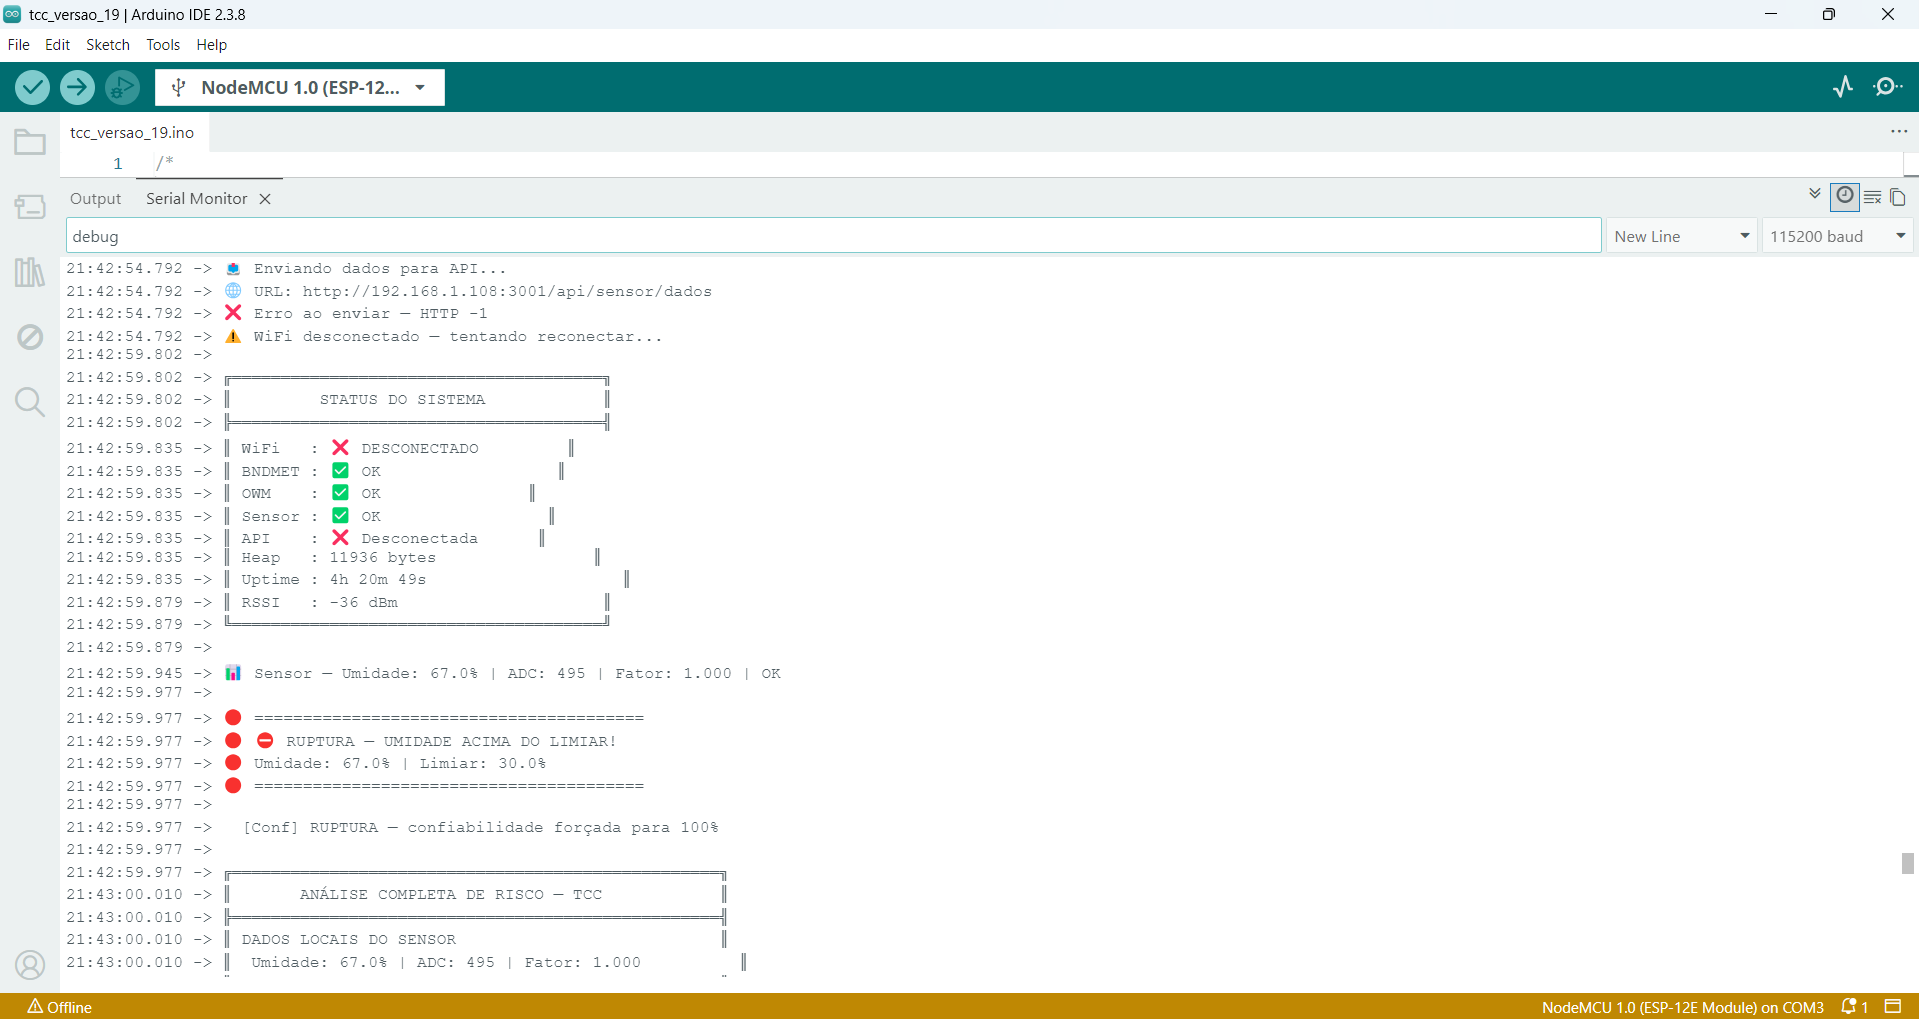
\includegraphics[width=0.85\textwidth]{figures/cap5_serial_ruptura_confiabilidade_100_pt1.png}
    \caption{Monitor serial durante ruptura ativa com API local indisponível (parte~1): estado de RUPTURA ativo com API local indisponível e fontes de dados disponíveis.}
    \label{fig:serial_ruptura_confiabilidade_100_pt1}
    \fonte{Elaborado pela autora.}
\end{figure}

\begin{figure}[htbp]
    \centering
    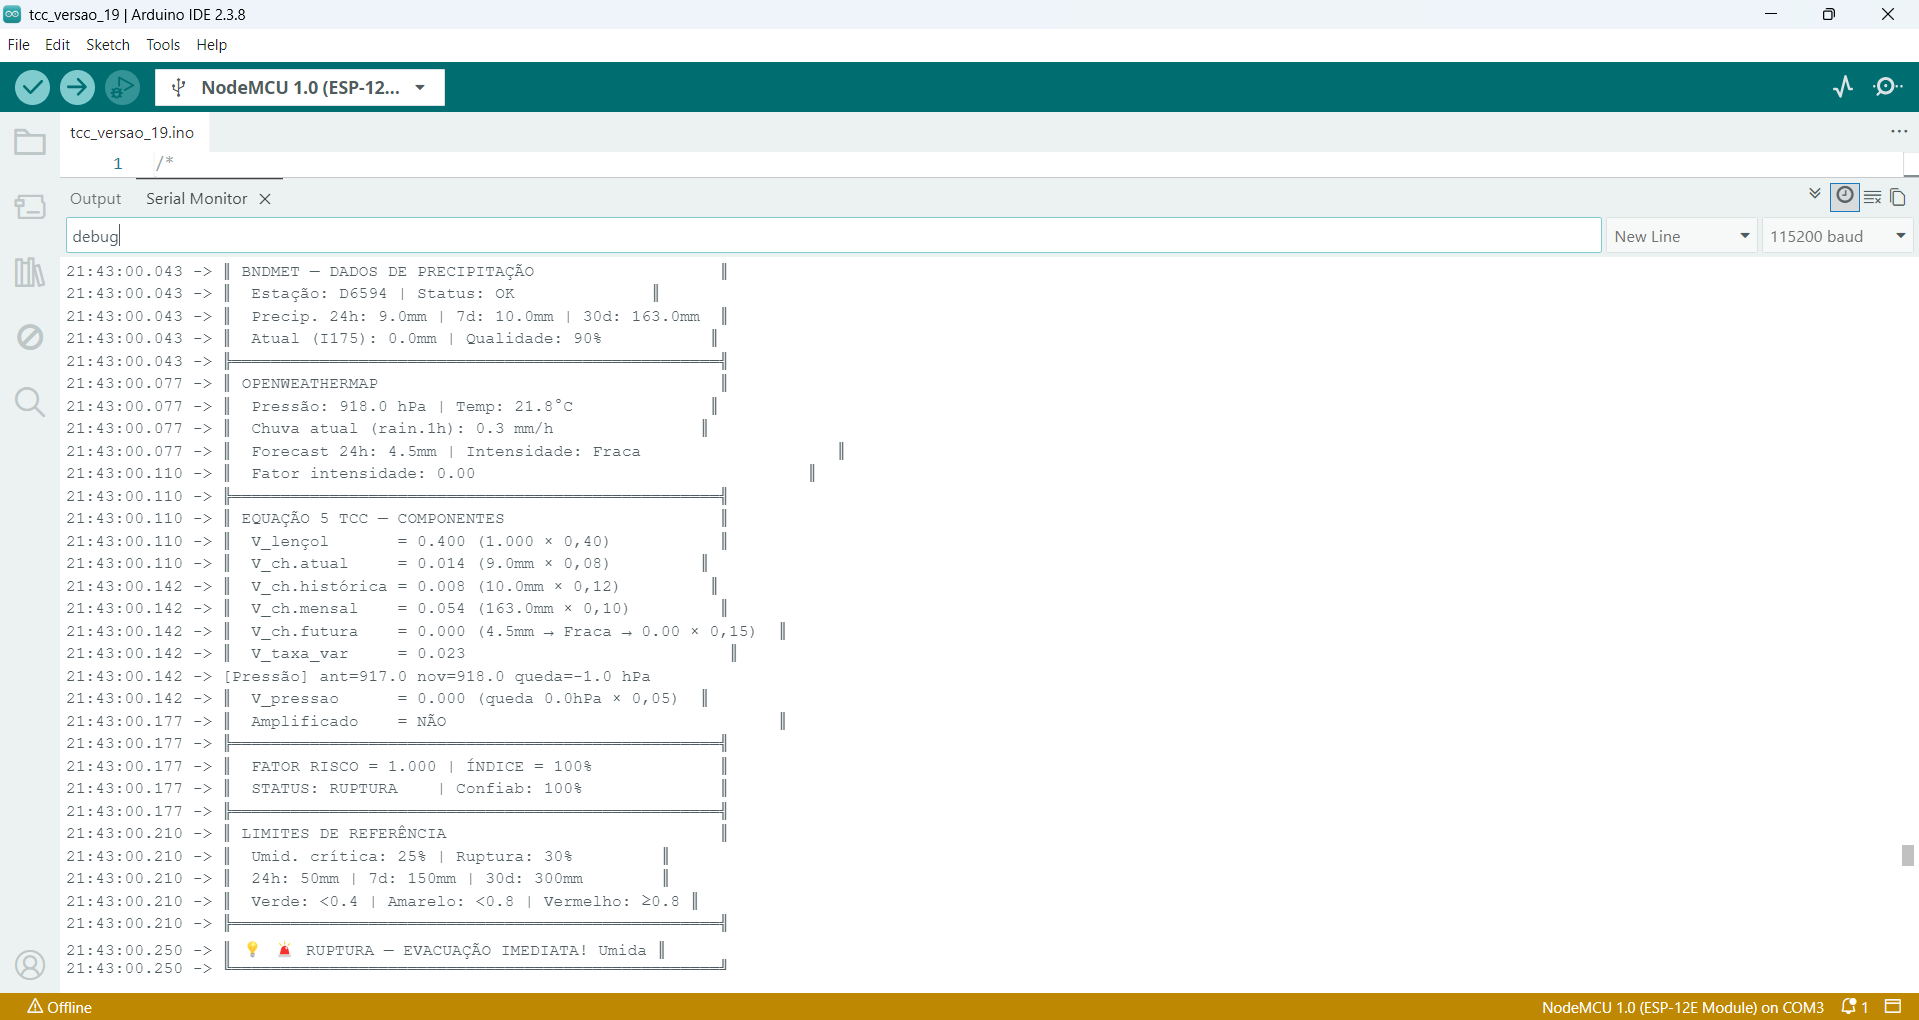
\includegraphics[width=0.85\textwidth]{figures/cap5_serial_ruptura_confiabilidade_100_pt2.png}
    \caption{Monitor serial durante ruptura ativa com API indisponível (parte~2): confiabilidade fixada em 100\% pelo estado especial de RUPTURA, sobrepondo todos os descontos que seriam aplicados.}
    \label{fig:serial_ruptura_confiabilidade_100_pt2}
    \fonte{Elaborado pela autora.}
\end{figure}

O \textit{firmware} implementa um mecanismo de supervisão periódica ---
executado a cada cinco minutos --- que monitora três condições de falha e
toma a ação corretiva correspondente a cada uma delas.

O primeiro gatilho atua sobre a conectividade Wi-Fi: a cada 30 segundos,
a função de verificação tenta reconectar o módulo à rede. Quando o número
de tentativas consecutivas sem sucesso ultrapassa dez, o dispositivo
executa uma reinicialização completa via \texttt{ESP.restart()},
garantindo que o sistema retorne a um estado inicial limpo, conforme
ilustra a \autoref{fig:serial_wifi_falha_envio}.

\begin{figure}[htbp]
    \centering
    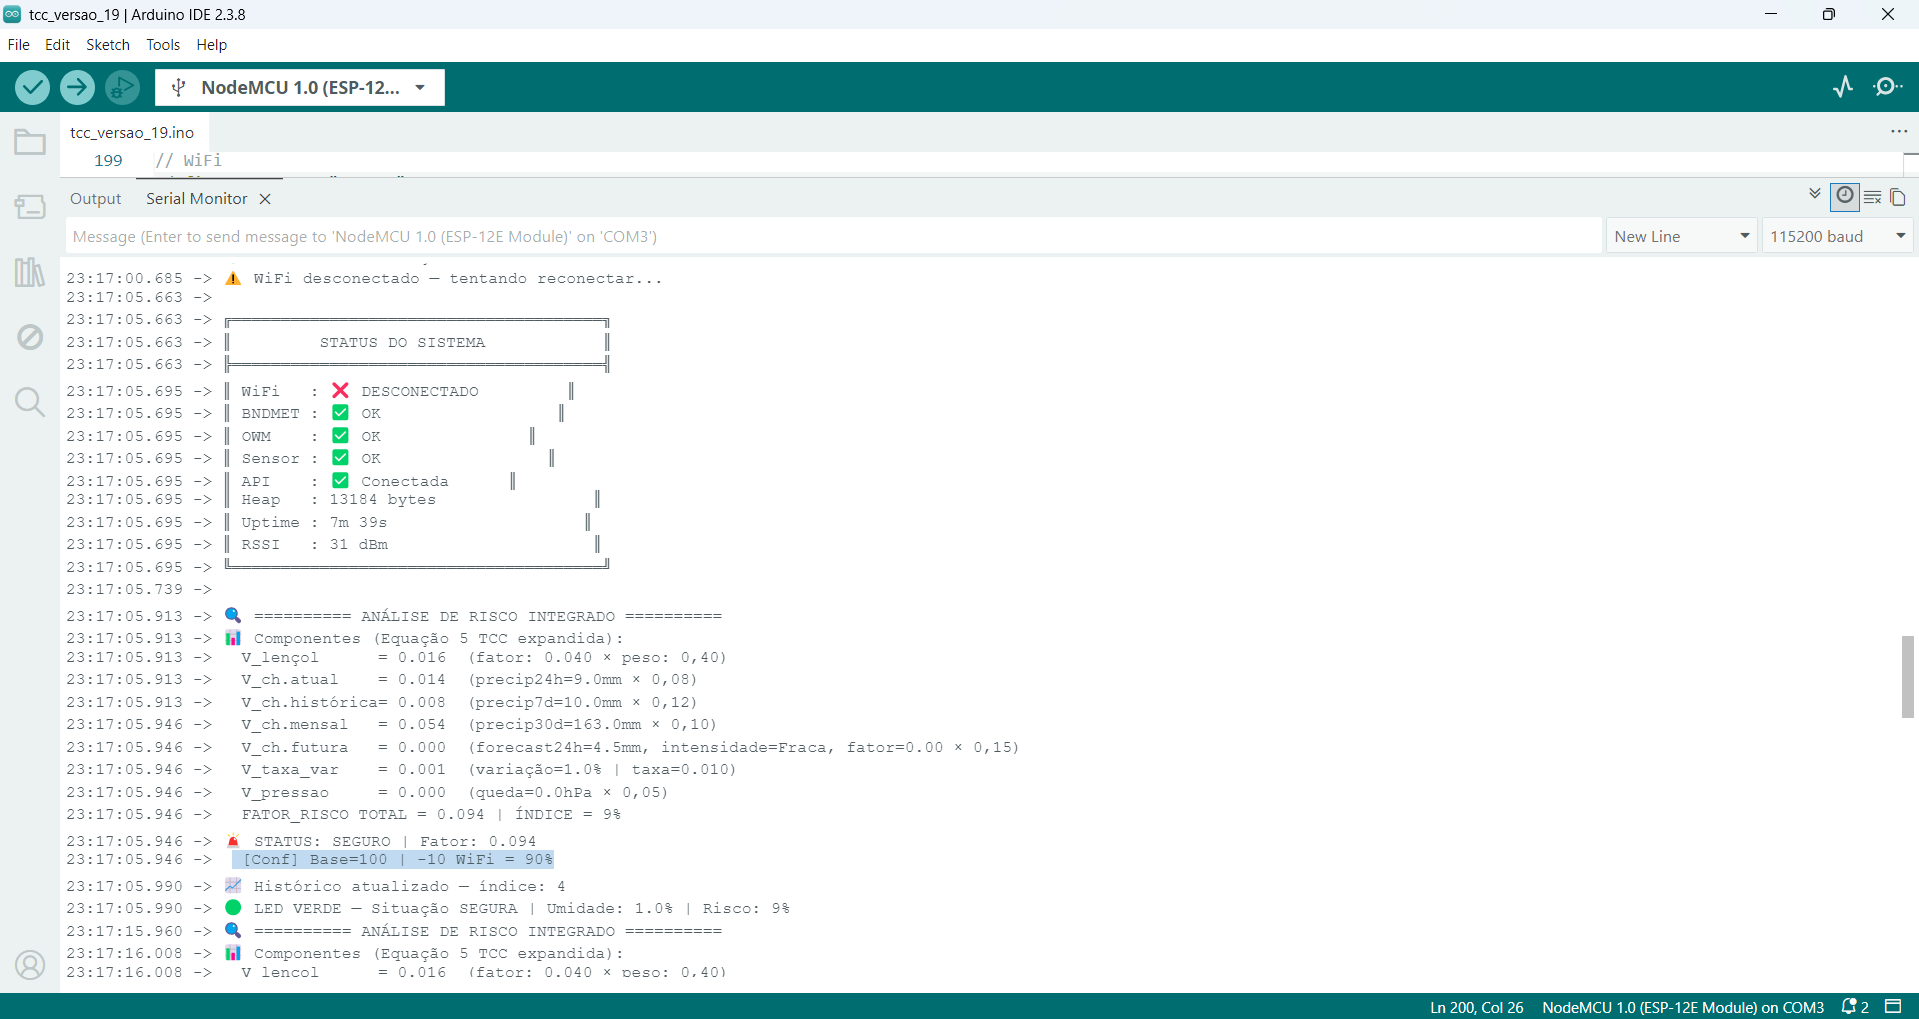
\includegraphics[width=0.85\textwidth]{figures/cap5_serial_wifi_falha_envio.png}
    \caption{Monitor serial durante falha persistente de Wi-Fi: tentativas
    de reconexão automática a cada 30 segundos e reinicialização completa
    do dispositivo ao atingir dez falhas consecutivas sem sucesso.}
    \label{fig:serial_wifi_falha_envio}
    \fonte{Elaborado pela autora.}
\end{figure}

O segundo gatilho atua sobre as falhas de comunicação com o
\textit{backend}: quando o contador de envios sem resposta ultrapassa dez
ocorrências consecutivas, o módulo Wi-Fi é desconectado e reconectado sem
reinicializar o dispositivo --- o contador é zerado e o sistema retoma as
tentativas de envio normalmente, conforme ilustra a
\autoref{fig:serial_backend_sem_resposta}.

\begin{figure}[htbp]
    \centering
    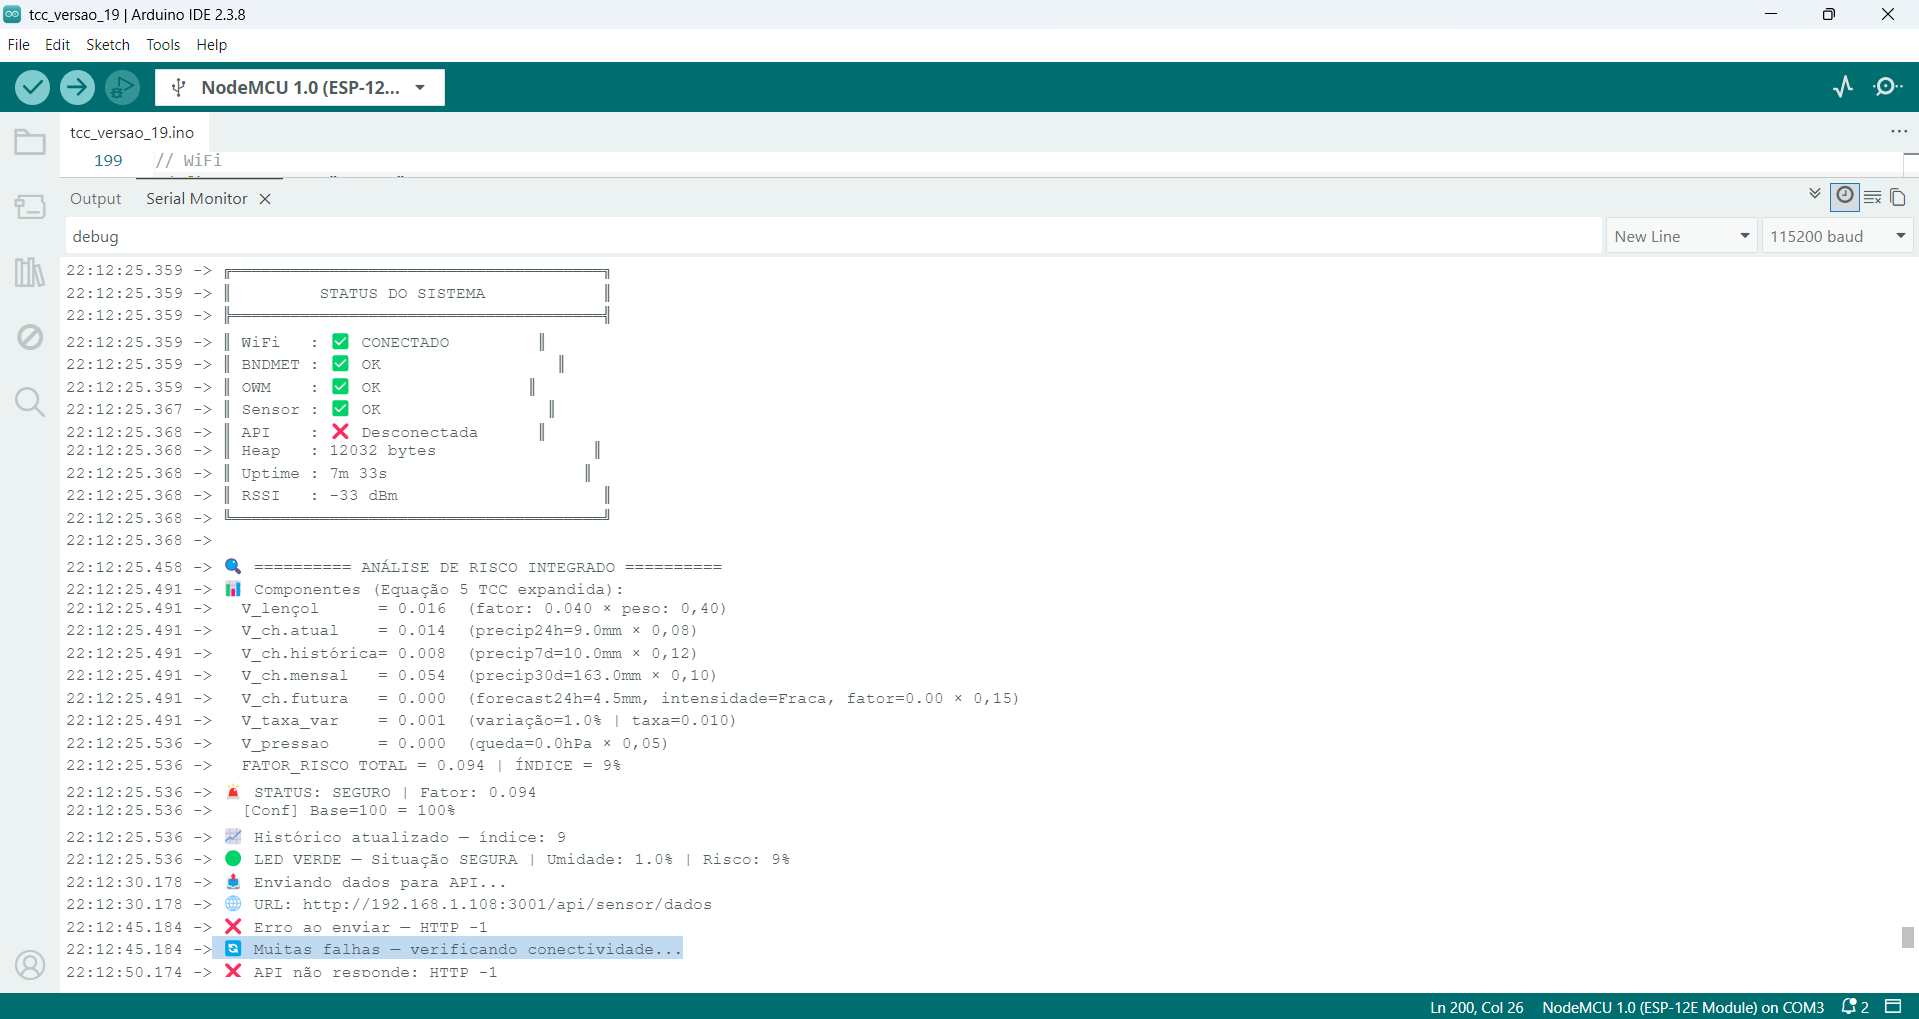
\includegraphics[width=0.85\textwidth]{figures/cap5_serial_backend_sem_resposta.png}
    \caption{Monitor serial com \textit{backend} sem resposta e Wi-Fi
    ativo: contador de falhas incrementado ciclo a ciclo e reconexão do
    módulo Wi-Fi ao atingir dez falhas consecutivas, sem reinicialização
    do dispositivo.}
    \label{fig:serial_backend_sem_resposta}
    \fonte{Elaborado pela autora.}
\end{figure}

O terceiro gatilho atua sobre a memória disponível: quando a
\textit{heap} livre cai abaixo de 5.000 bytes, o dispositivo reinicia
automaticamente para prevenir travamentos por esgotamento de memória,
conforme demonstra a \autoref{fig:serial_heap_critico}.

\begin{figure}[htbp]
    \centering
    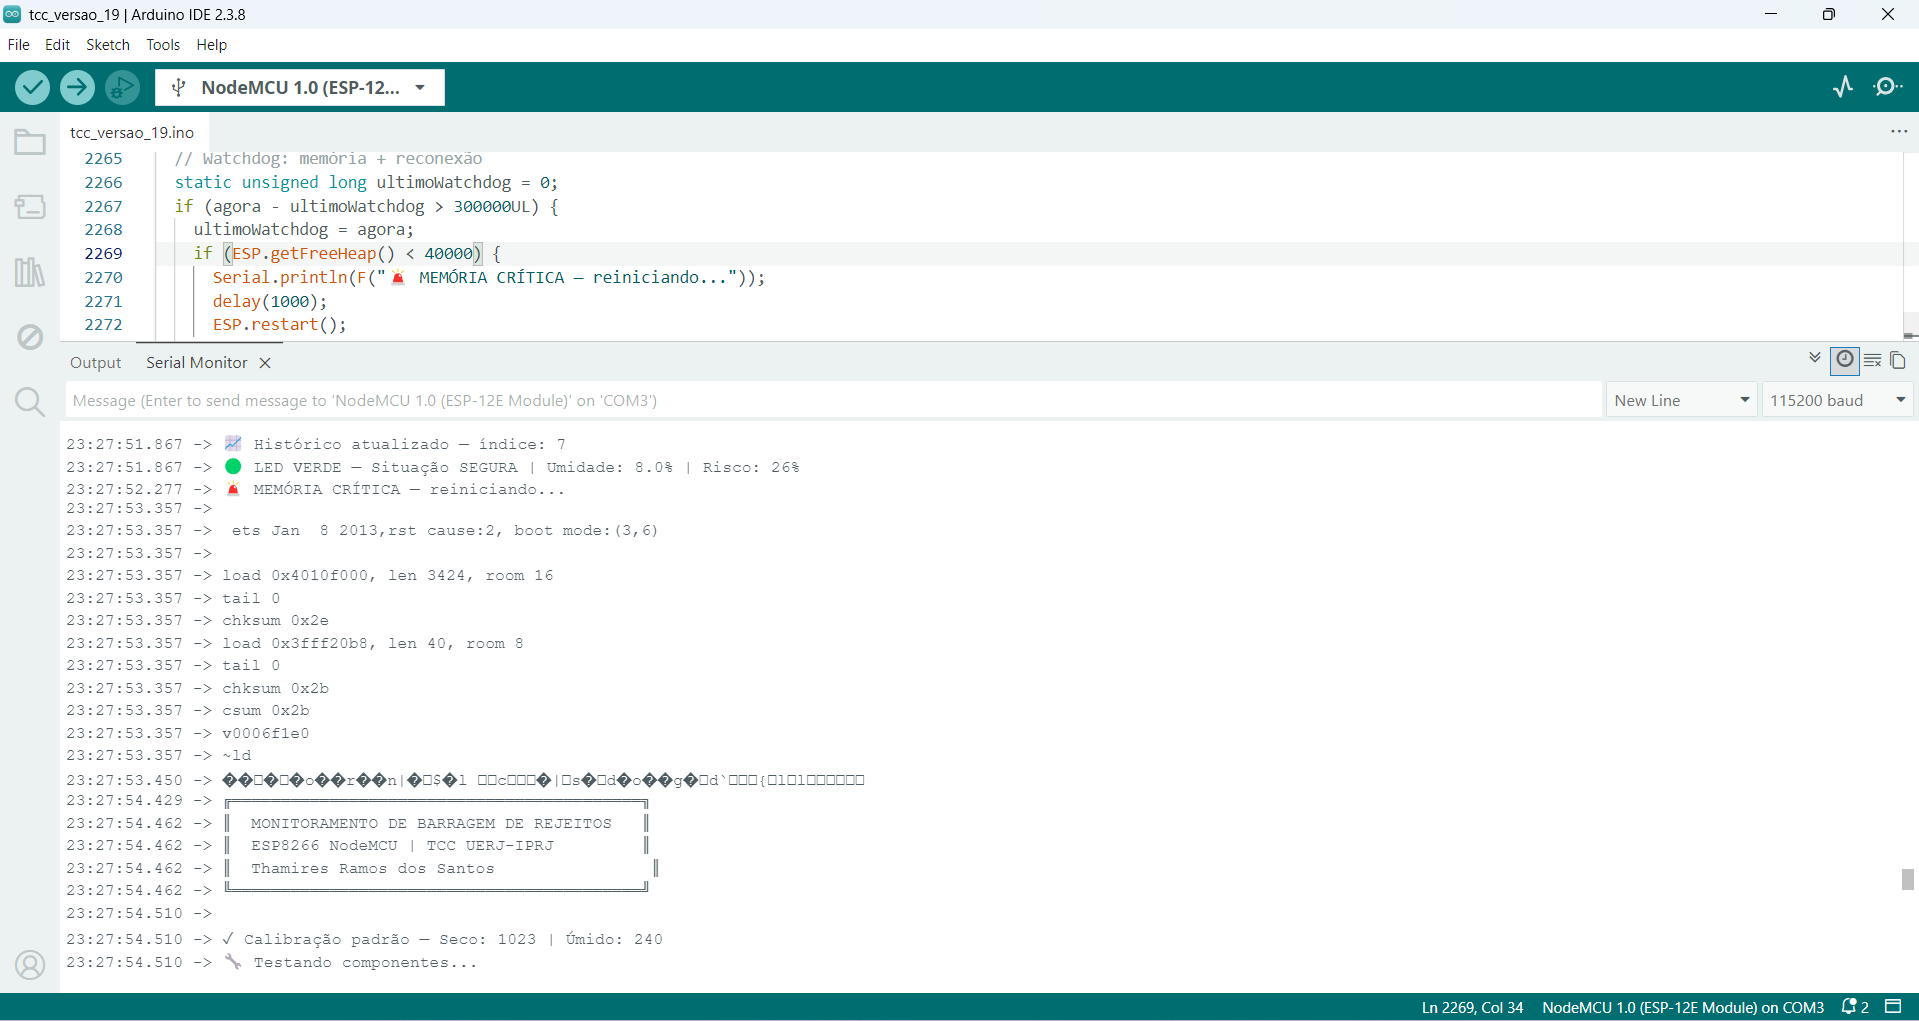
\includegraphics[width=0.85\textwidth]{figures/cap5_serial_heap_critico.png}
    \caption{Monitor serial com \textit{heap} crítico detectado: memória
    livre abaixo de 5.000 bytes e reinicialização automática do
    dispositivo.}
    \label{fig:serial_heap_critico}
    \fonte{Elaborado pela autora.}
\end{figure}

% -------------------------------------------------------------
\subsection{Protocolo de Ruptura}
\label{subsec:ruptura}
% -------------------------------------------------------------

Quando a umidade do solo atinge ou supera 30\%, o sistema aciona o
protocolo de ruptura de forma imediata, sem aguardar o próximo ciclo
de análise programado. O monitor serial exibe o banner de emergência
mostrado na \autoref{fig:serial_ruptura}: a umidade registrada, o limiar
ultrapassado e a mensagem de evacuação imediata. O LED vermelho acende
e o \textit{buzzer} dispara na frequência máxima de 2.400\,Hz,
independentemente do índice calculado pelos componentes do modelo.

\begin{figure}[htbp]
    \centering
    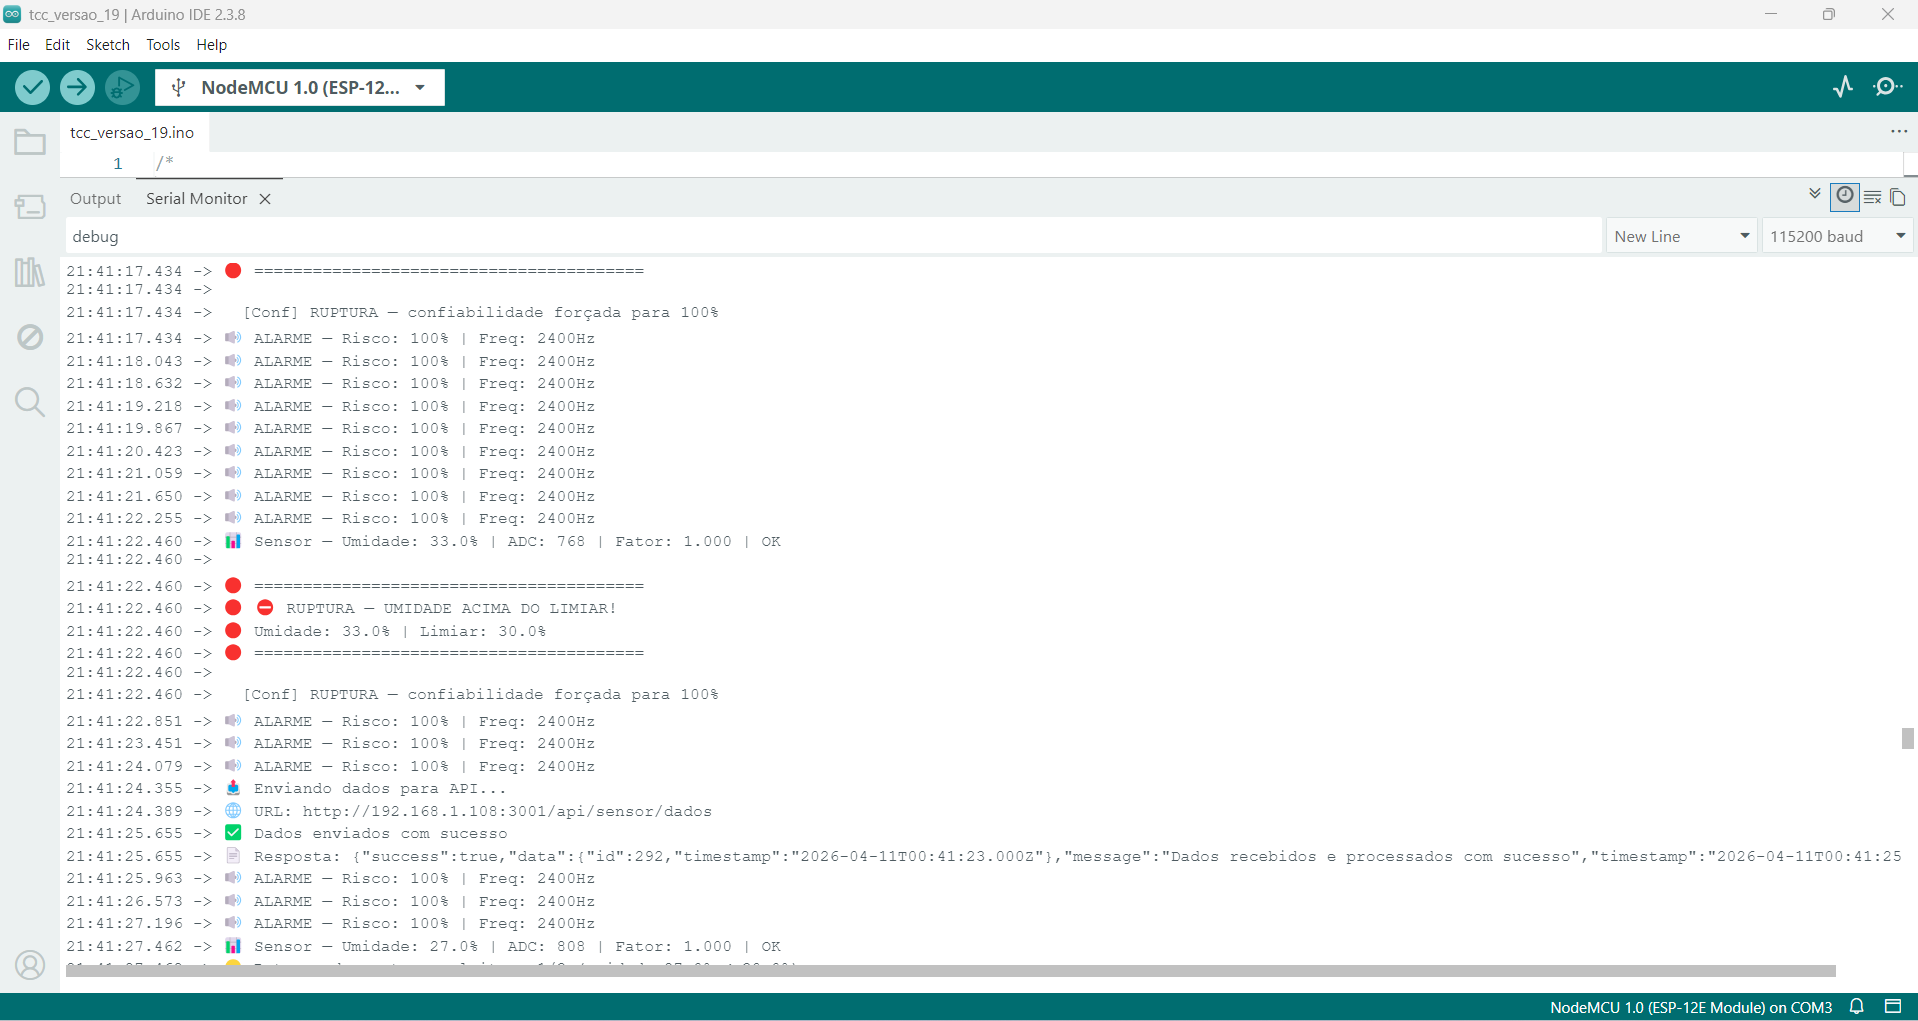
\includegraphics[width=0.85\textwidth]{figures/cap5_serial_ruptura.png}
    \caption{Monitor serial no acionamento do protocolo de ruptura: umidade
    acima de 30\%, LED vermelho e \textit{buzzer} em 2.400\,Hz acionados
    imediatamente, mensagem de evacuação exibida.}
    \label{fig:serial_ruptura}
    \fonte{Elaborado pela autora.}
\end{figure}

Assim que a umidade retorna abaixo de 30\%, inicia-se o período de
\textit{cooldown}: o sistema aguarda três leituras consecutivas com
valores seguros antes de retomar o cálculo normal de risco. Durante esse
intervalo, o monitor serial exibe a contagem progressiva de cada leitura
segura --- ``Retorno de ruptura --- leitura 1/3'', ``leitura 2/3'' e
``leitura 3/3'' --- até a mensagem ``RUPTURA ENCERRADA'' confirmar o
retorno ao fluxo normal, conforme ilustrado na
\autoref{fig:serial_cooldown}. Esse mecanismo de três confirmações
consecutivas protege o sistema contra oscilações na leitura do sensor
imediatamente após o pico de umidade.

\begin{figure}[htbp]
    \centering
    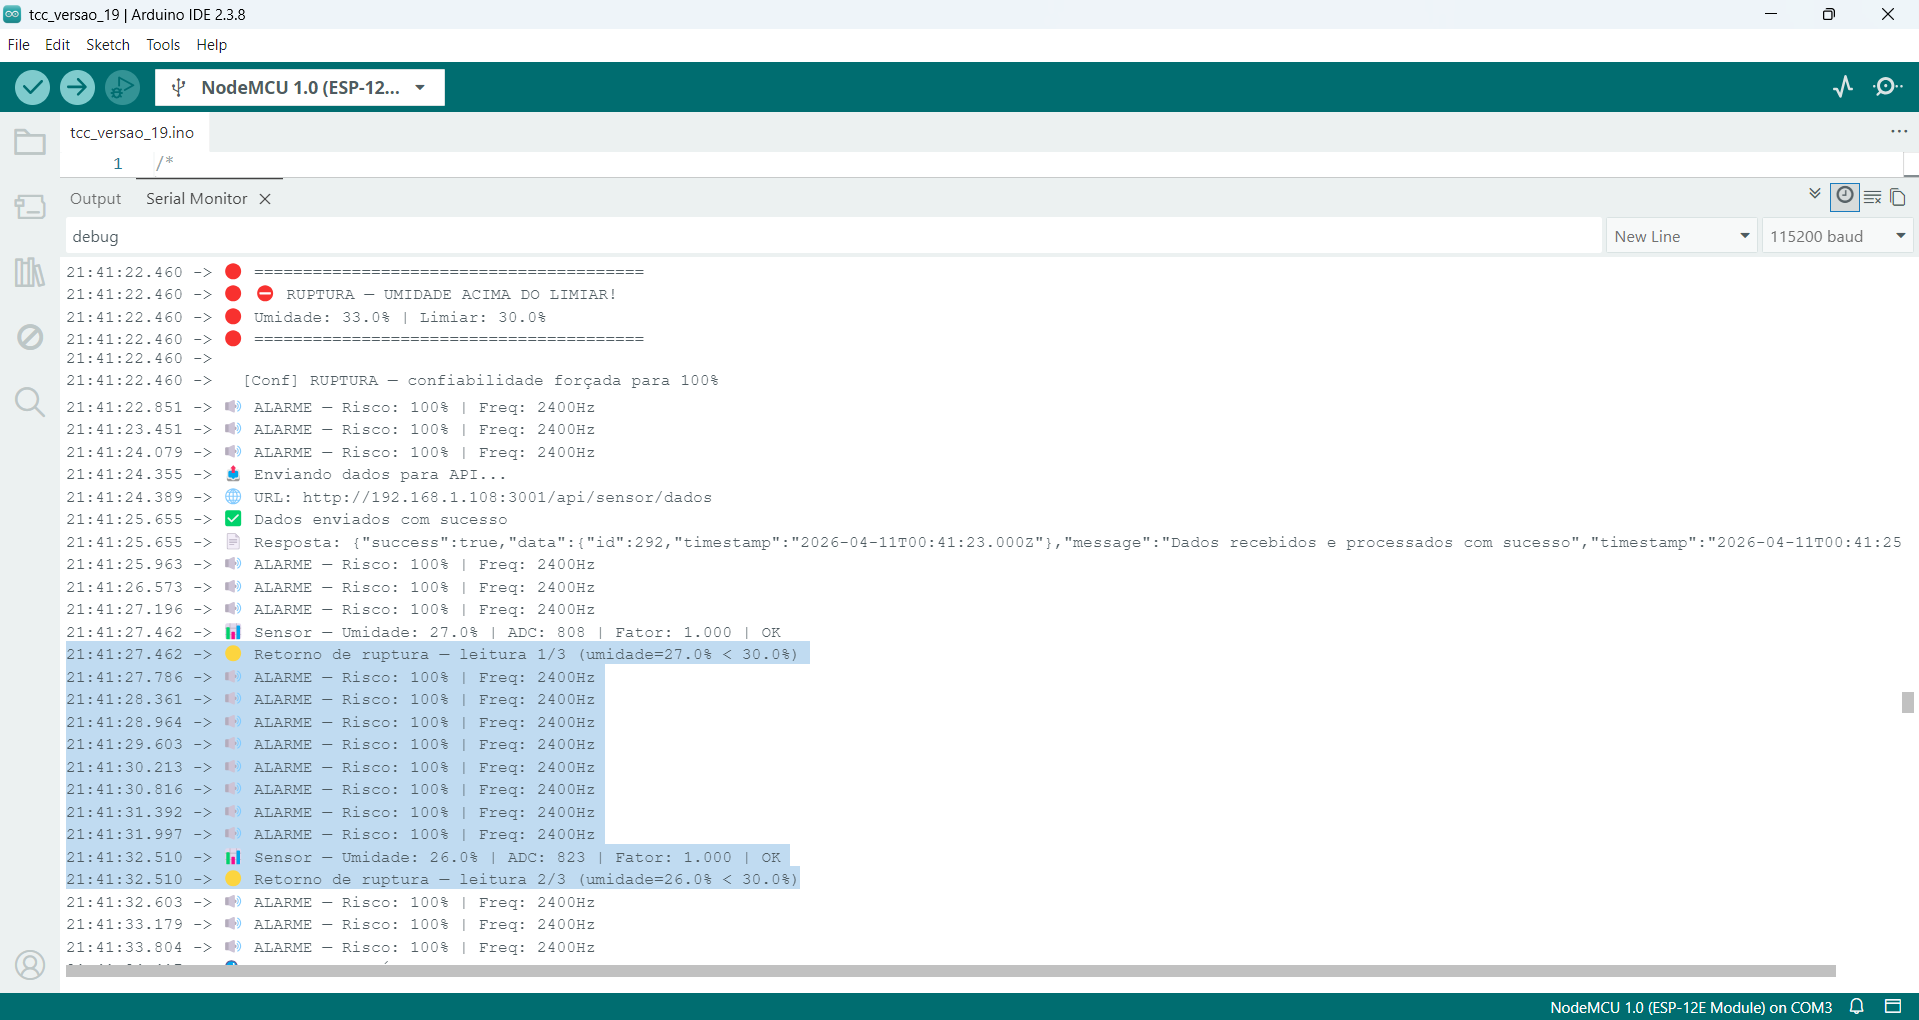
\includegraphics[width=0.85\textwidth]{figures/cap5_serial_cooldown.png}
    \caption{Monitor serial durante o \textit{cooldown} de ruptura:
    contagem das três leituras consecutivas com umidade abaixo de 30\%
    e confirmação do encerramento do estado de ruptura.}
    \label{fig:serial_cooldown}
    \fonte{Elaborado pela autora.}
\end{figure}

% -------------------------------------------------------------
\subsection{Comandos via Serial Monitor}
\label{subsec:serial}
% -------------------------------------------------------------

O dispositivo disponibiliza onze comandos acessíveis pelo monitor serial
do Arduino IDE durante a operação, listados na
\autoref{tab:comandos_serial}. Os três comandos de simulação de nível
(\texttt{alerta verde}, \texttt{alerta amarelo} e \texttt{alerta
vermelho}) foram especialmente úteis durante os testes: ao forçar um
nível específico, é possível observar a resposta dos LEDs, o comportamento
do \textit{buzzer} e a alteração do intervalo de envio ao
\textit{backend} sem aguardar condições naturais que acionem o alerta.
Cada simulação realiza exatamente três envios ao \textit{backend} com os
dados do nível forçado e, ao concluir o terceiro envio, encerra-se
automaticamente: as \textit{flags} \texttt{simulacaoAtiva} e
\texttt{modoManual} retornam a \texttt{false}, o \textit{buzzer} é
silenciado e o sistema retorna ao modo automático sem intervenção do
operador. Durante toda a simulação, a leitura do higrômetro é suspensa
--- a função \texttt{atualizarDadosLocais()} retorna imediatamente
quando \texttt{modoManual = true} --- garantindo que nenhuma leitura
real sobrescreva os valores forçados antes que os três envios sejam
concluídos. Quando um comando não reconhecido é digitado, o sistema
responde com ``Comando não reconhecido. Digite \texttt{help}'', conforme
ilustra a \autoref{fig:serial_comando_nao_reconhecido}.

\begin{figure}[htbp]
    \centering
    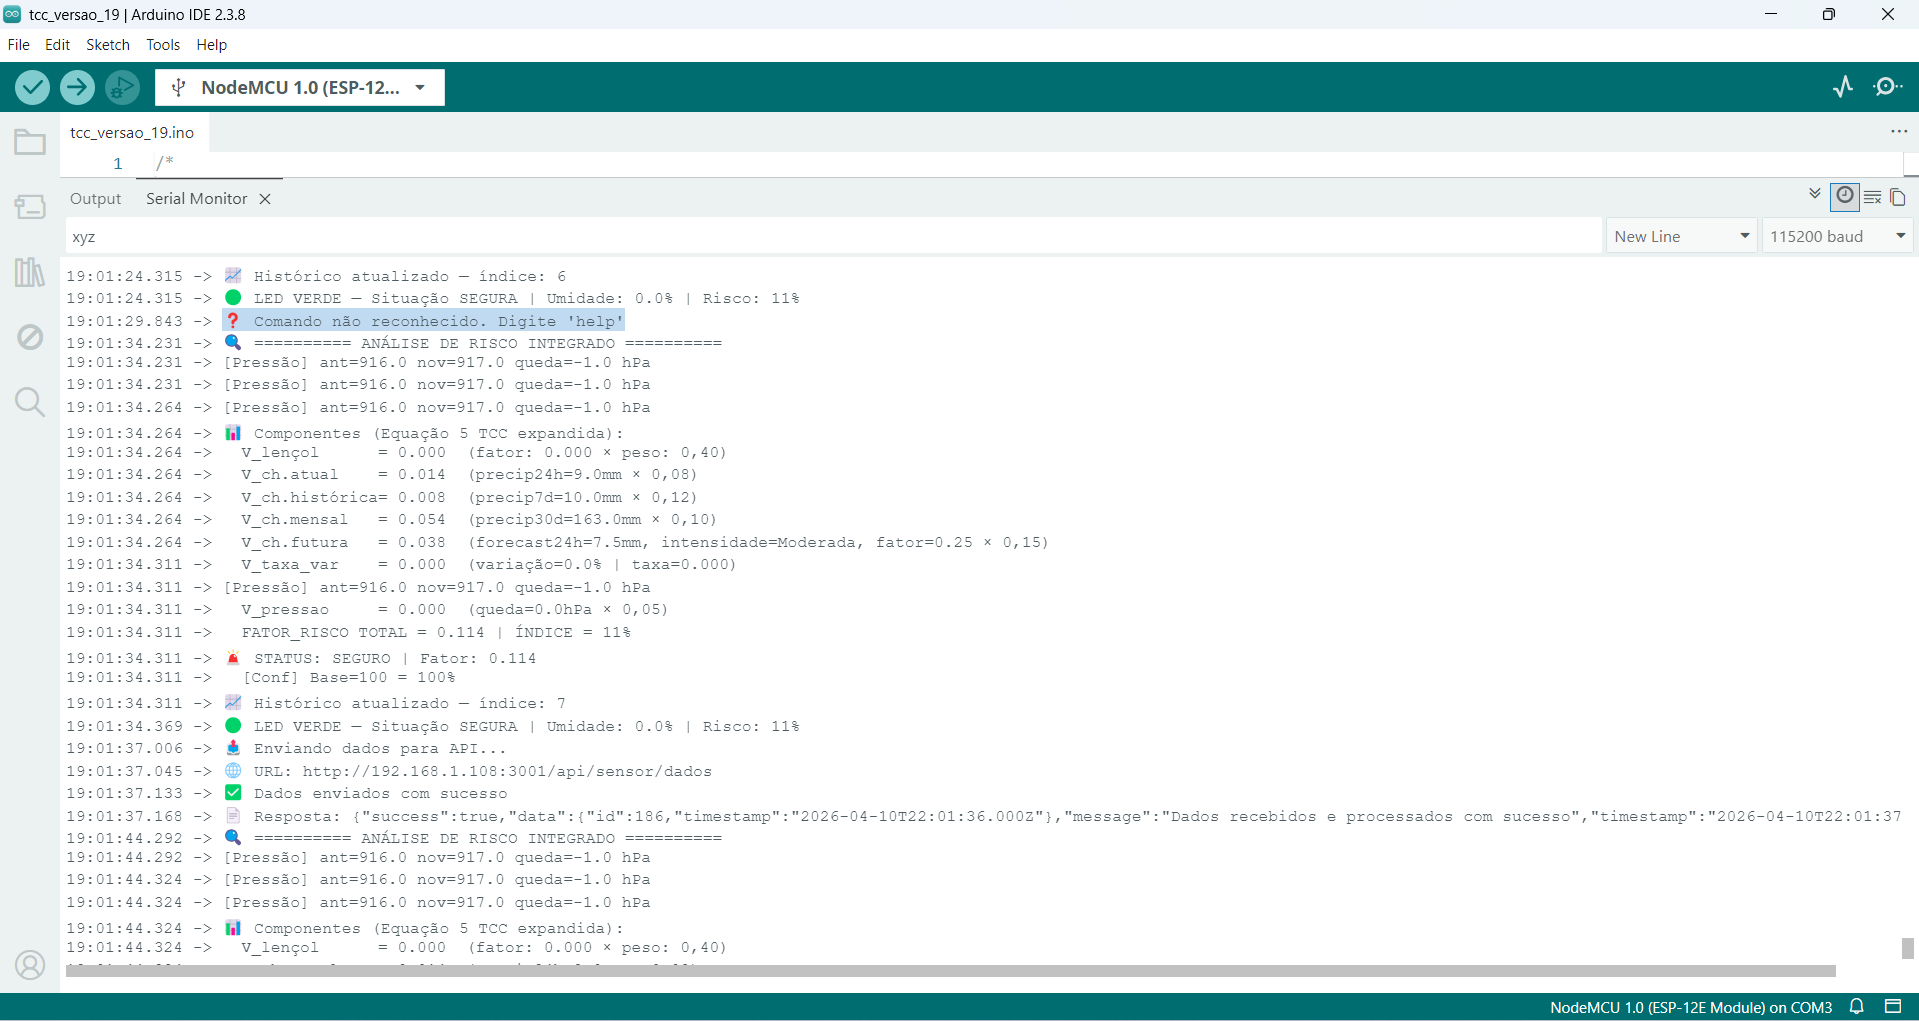
\includegraphics[width=0.85\textwidth]{figures/cap5_serial_comando_nao_reconhecido.png}
    \caption{Monitor serial com comando não reconhecido digitado: resposta ``Comando não reconhecido. Digite \texttt{help}'' exibida imediatamente, sem interromper o ciclo de operação do sistema.}
    \label{fig:serial_comando_nao_reconhecido}
    \fonte{Elaborado pela autora.}
\end{figure}

\begin{table}[htb]
\centering
\caption{Comandos disponíveis via Serial Monitor e resultados observados}
\label{tab:comandos_serial}
\begin{tabular}{lp{9.5cm}}
\hline
\textbf{Comando} & \textbf{Resultado observado} \\
\hline
\texttt{status}          & Painel com estado de Wi-Fi, BNDMET, OWM, sensor, \textit{backend}, memória livre, \textit{uptime} e RSSI \\
\texttt{analise}         & Executa imediatamente um ciclo de análise com os dados em memória \\
\texttt{debug}           & Painel detalhado com os sete componentes do modelo, fator de risco integrado, nível, confiabilidade e recomendação \\
\texttt{calibrar}        & Inicia recalibração: solicita leituras em solo seco e saturado e persiste os novos valores na EEPROM \\
\texttt{reset}           & Apaga LEDs e \textit{buzzer}, reinicia estruturas de memória e reinicia o dispositivo após 3 segundos \\
\texttt{teste}           & Rotina de sete etapas: \textit{hardware}, conectividade, sensor, BNDMET, OWM, cálculos e análise \\
\texttt{enviar}          & Força envio imediato dos dados em memória ao \textit{backend} \\
\texttt{api}             & Testa conectividade com o \textit{backend} e exibe ``API OK'' ou ``API falha'' \\
\texttt{help}            & Exibe lista completa de comandos disponíveis \\
\texttt{alerta verde}    & Força nível VERDE; LED azul acende; intervalo de envio: 60 s \\
\texttt{alerta amarelo}  & Força nível AMARELO; LED amarelo acende; intervalo de envio: 20 s \\
\texttt{alerta vermelho} & Força nível VERMELHO; LED vermelho acende; \textit{buzzer} ativa; envio: 10 s \\
\hline
\end{tabular}
\fonte{Elaborado pela autora.}
\end{table}

As \autoref{fig:serial_comando_teste_pt1},
\autoref{fig:serial_comando_teste_pt2} e
\autoref{fig:serial_comando_teste_pt3} exibem a saída do comando \texttt{teste}, que percorre as sete etapas de verificação sequencialmente e reporta o resultado de cada uma.

\begin{figure}[htbp]
    \centering
    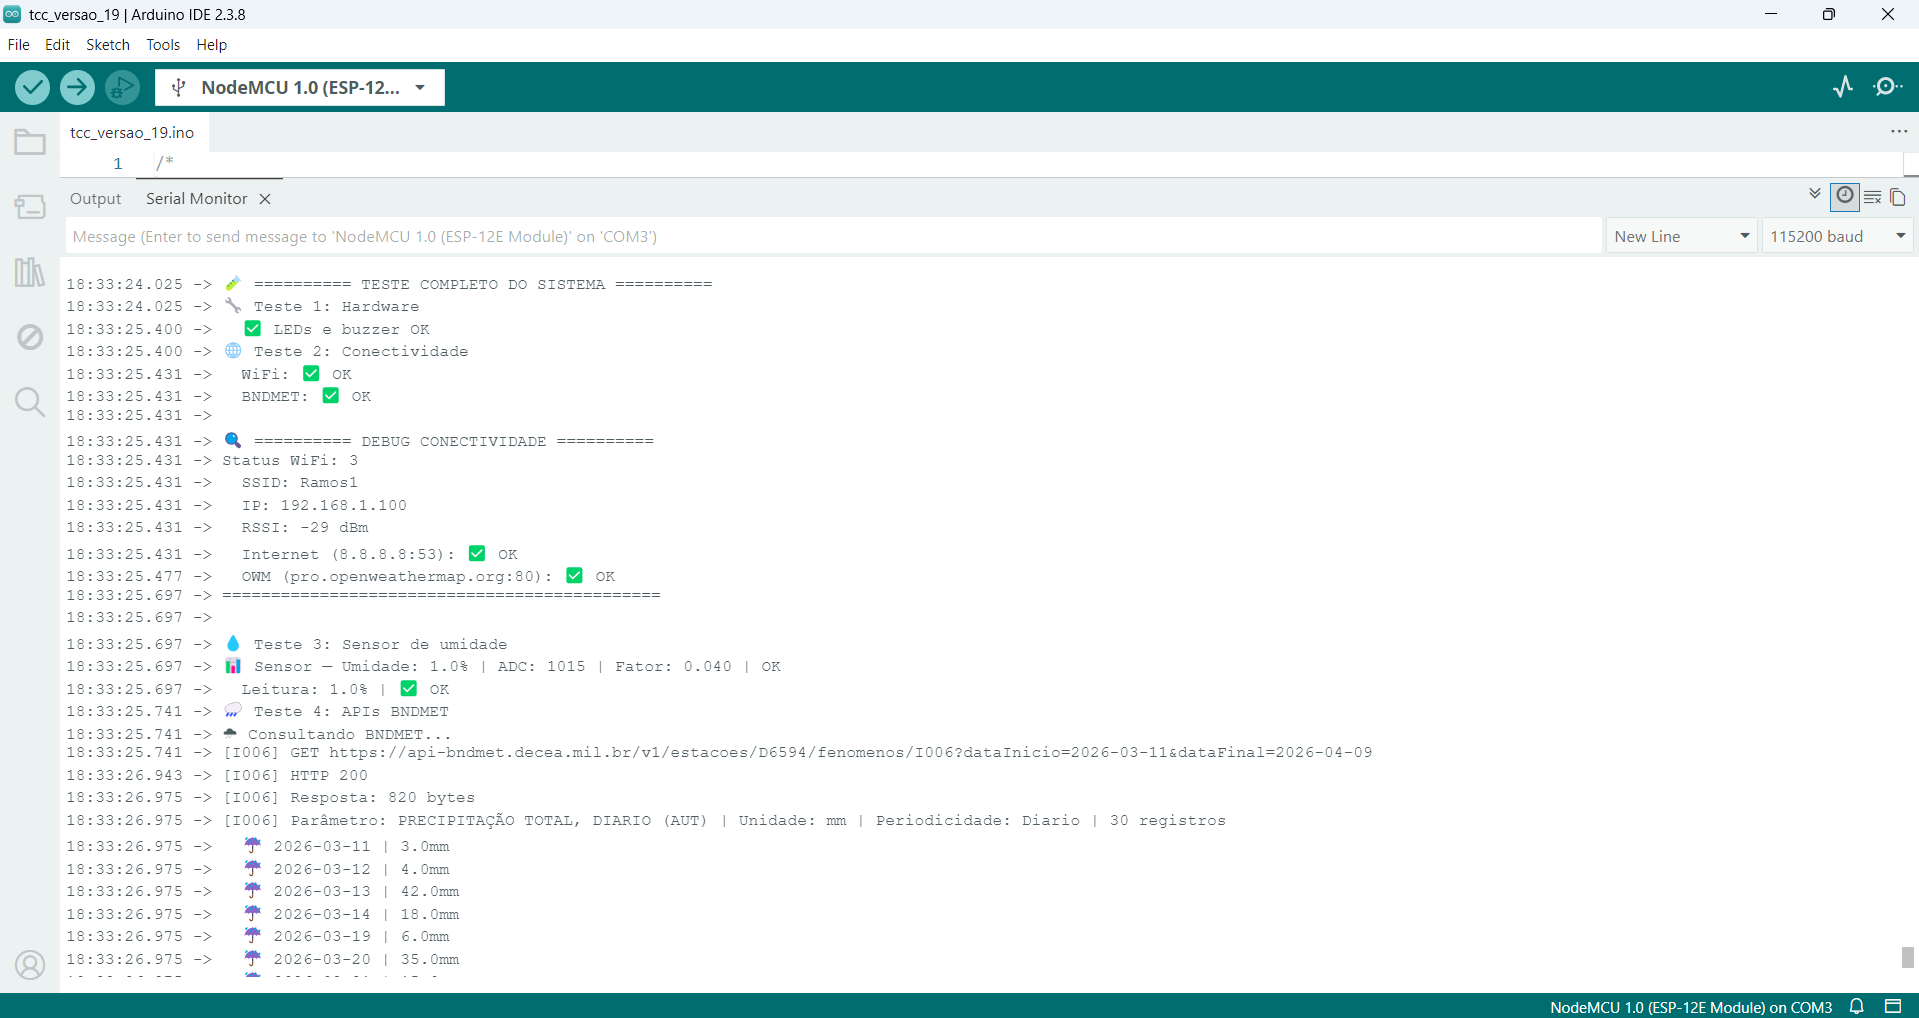
\includegraphics[width=0.85\textwidth]{figures/cap5_serial_comando_teste_pt1.png}
    \caption{Monitor serial durante execução do comando \texttt{teste} (parte~1): verificação de \textit{hardware} e conectividade.}
    \label{fig:serial_comando_teste_pt1}
    \fonte{Elaborado pela autora.}
\end{figure}

\begin{figure}[htbp]
    \centering
    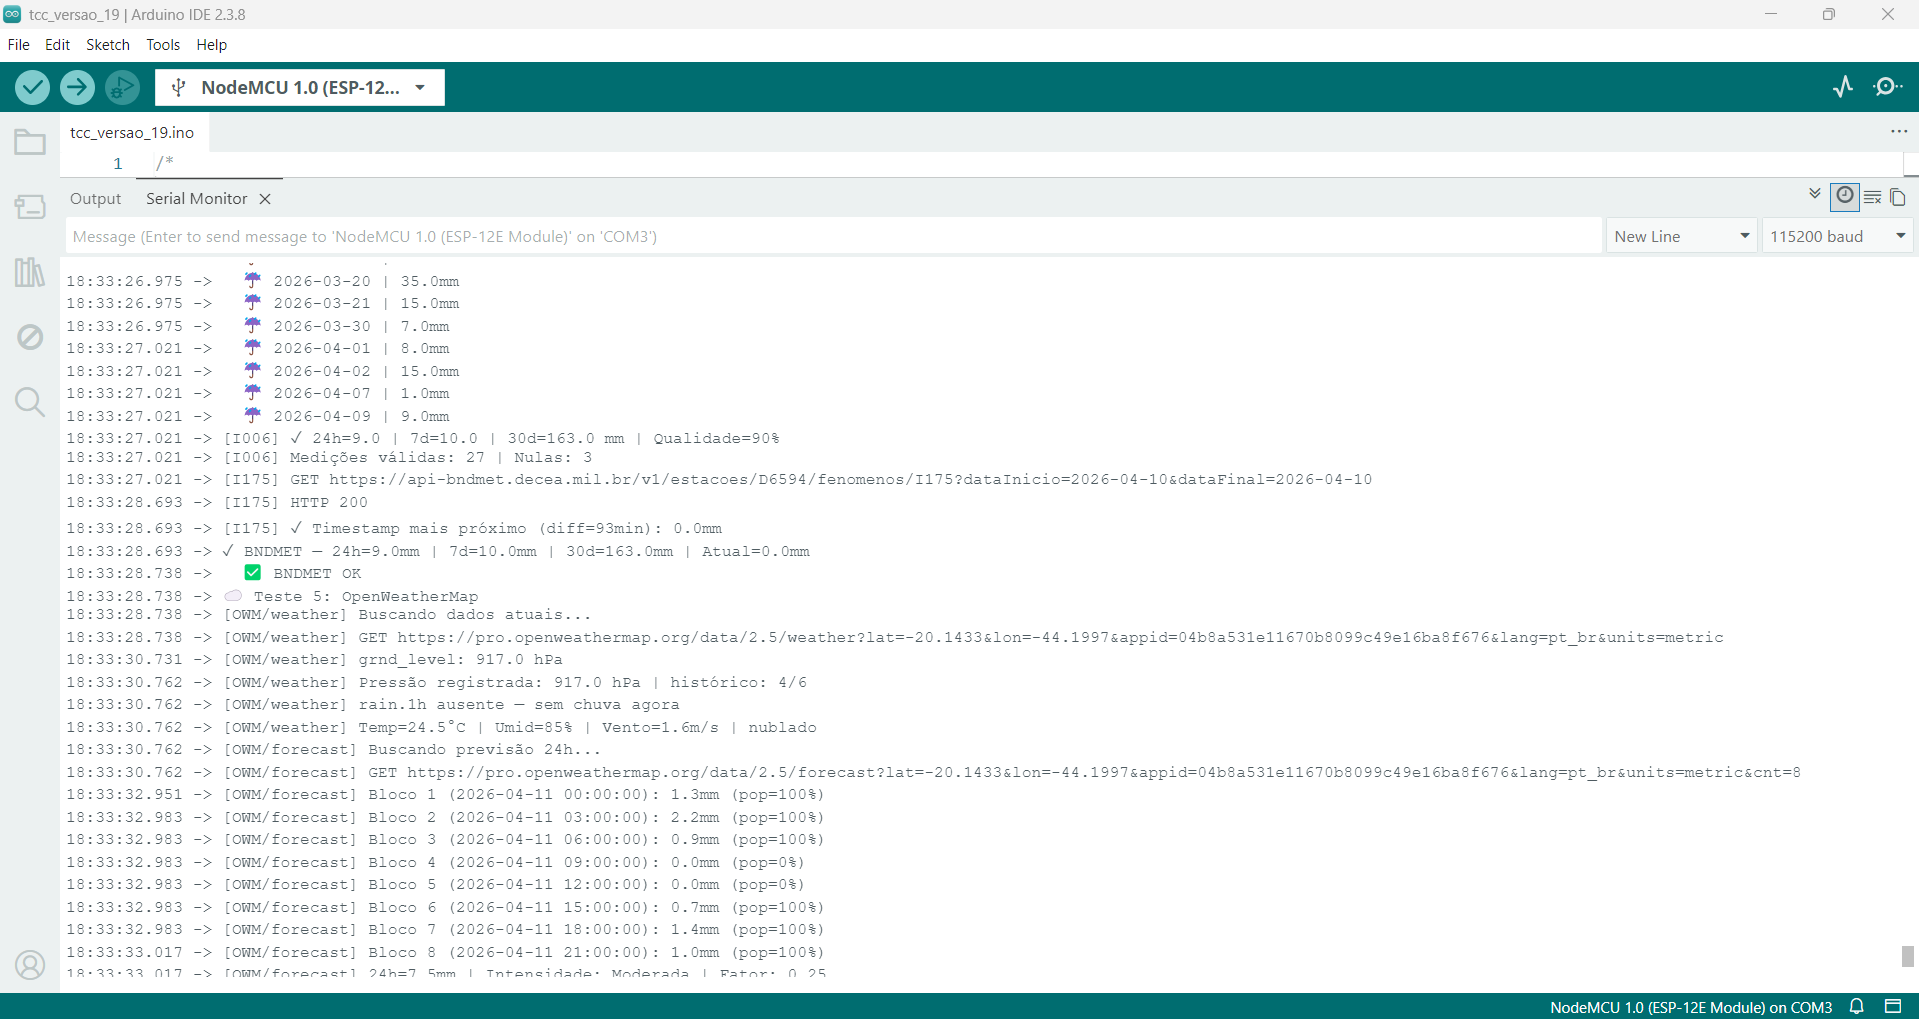
\includegraphics[width=0.85\textwidth]{figures/cap5_serial_comando_teste_pt2.png}
    \caption{Monitor serial durante execução do comando \texttt{teste} (parte~2): verificação do sensor, BNDMET e OWM.}
    \label{fig:serial_comando_teste_pt2}
    \fonte{Elaborado pela autora.}
\end{figure}

\begin{figure}[htbp]
    \centering
    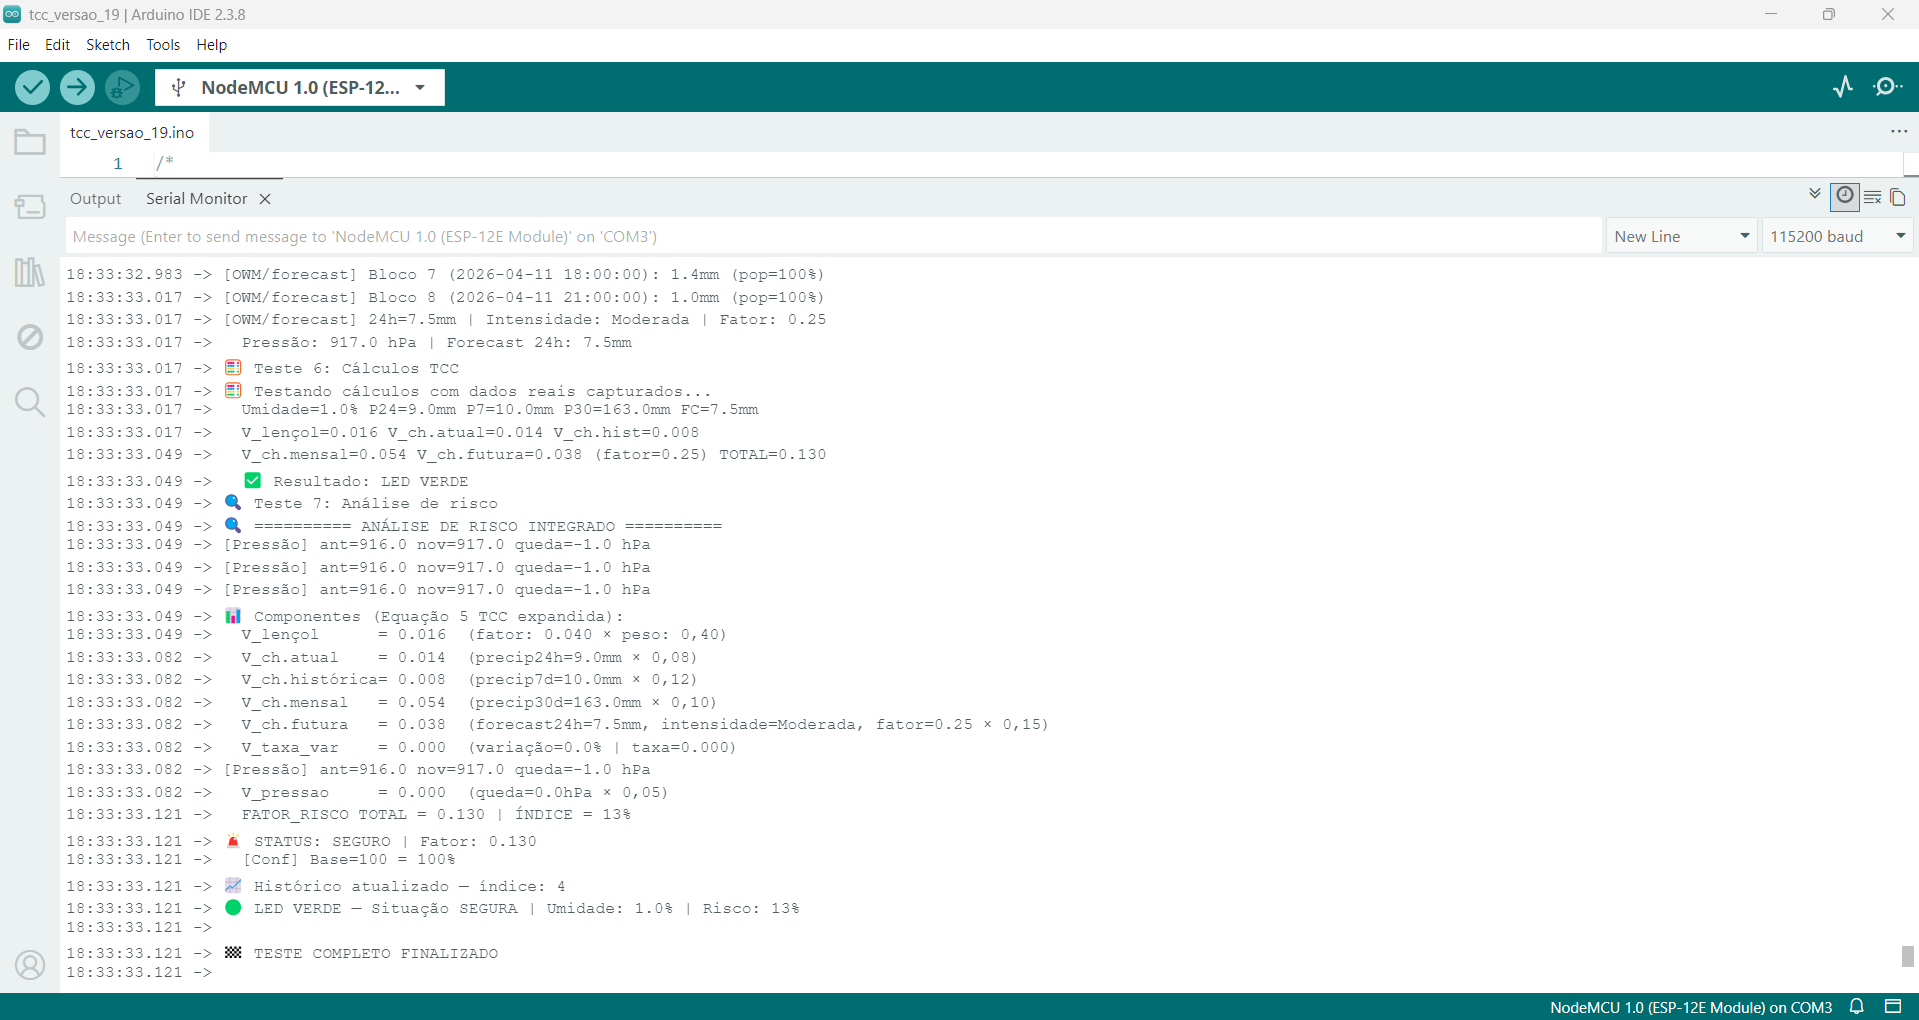
\includegraphics[width=0.85\textwidth]{figures/cap5_serial_comando_teste_pt3.png}
    \caption{Monitor serial durante execução do comando \texttt{teste} (parte~3): verificação de cálculos e análise de risco, com resultado individual de cada etapa.}
    \label{fig:serial_comando_teste_pt3}
    \fonte{Elaborado pela autora.}
\end{figure}

% =============================================================
\section{Interface \textit{Web} --- Autenticação}
\label{sec:autenticacao}
% =============================================================

% -------------------------------------------------------------
\subsection{Cadastro para Receber Alertas}
\label{subsec:landing-cadastro}
% -------------------------------------------------------------

A porta de entrada pública do sistema é a \textit{landing page}, acessível
sem autenticação. Nela, qualquer pessoa pode conhecer as funcionalidades
da plataforma e se cadastrar para receber notificações de alerta. A
\autoref{fig:landing_page_pt1} e \autoref{fig:landing_page_pt2} exibem a tela com o cabeçalho de identificação
do sistema, a seção de apresentação e os dois botões principais: ``Login''
--- para administradores --- e ``Cadastrar para Receber Alertas'' ---
para o público em geral.

\begin{figure}[htbp]
    \centering
    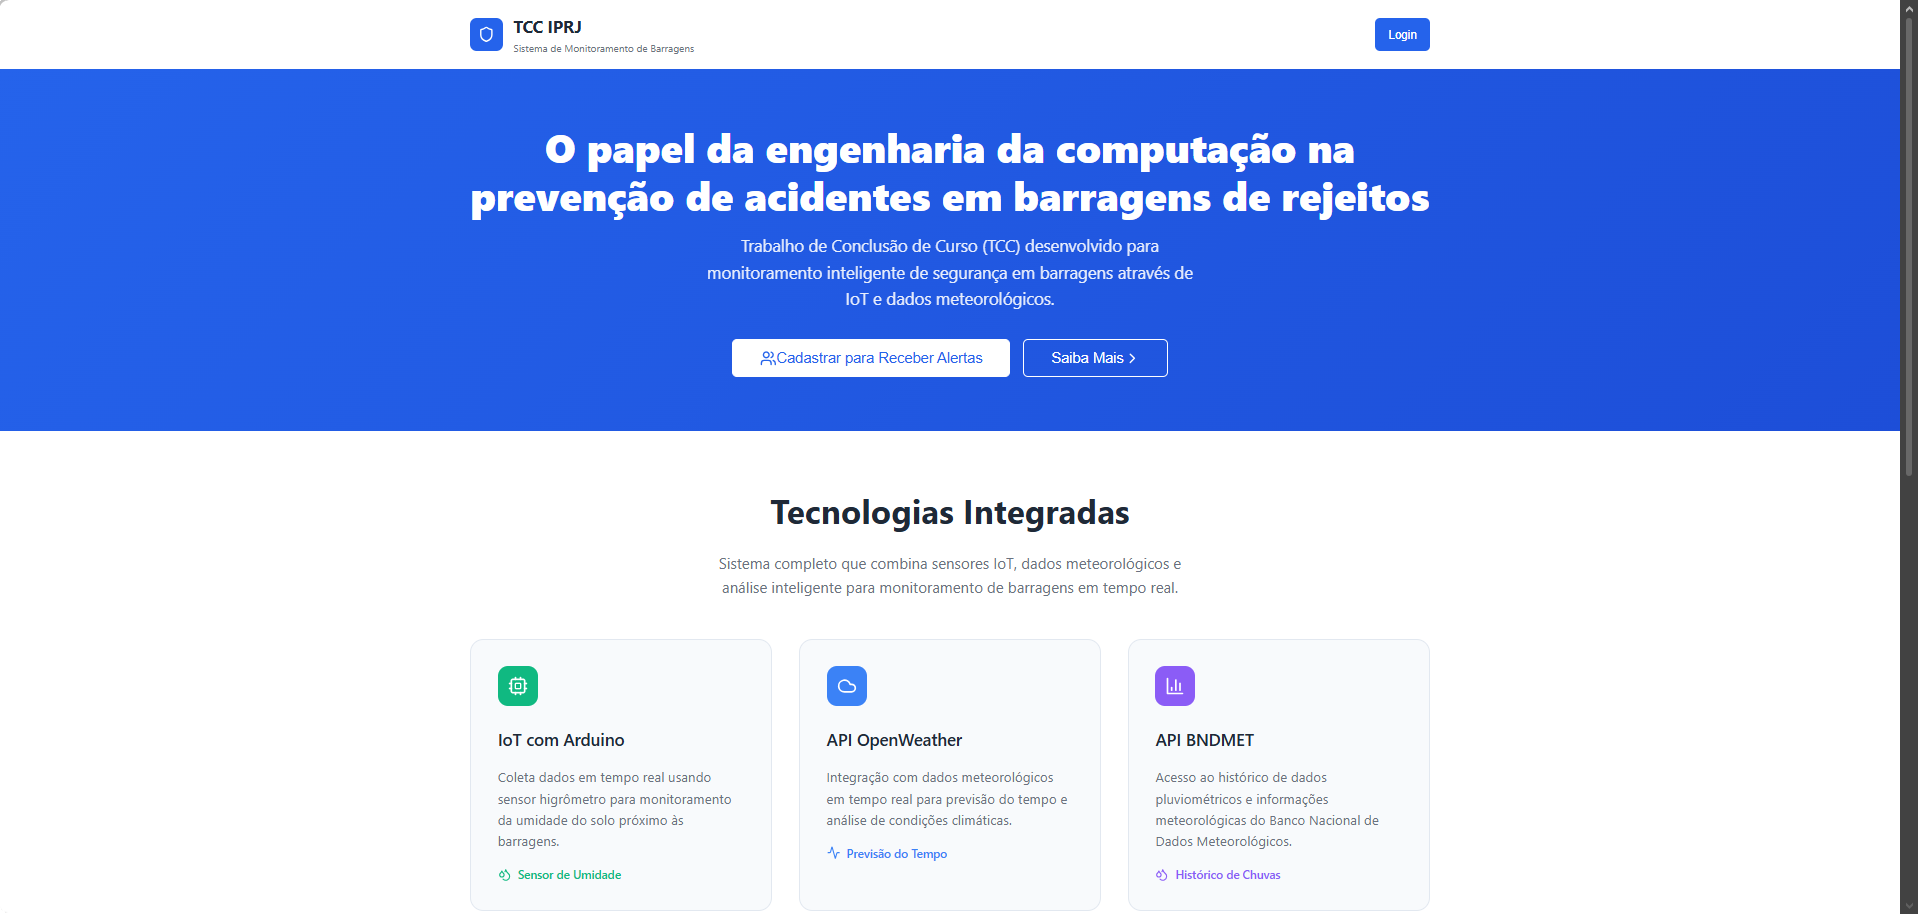
\includegraphics[width=0.95\textwidth]{figures/cap5_landing_page_pt1.png}
    \caption{\textit{Landing page} do sistema: cabeçalho com identificação,
    apresentação das funcionalidades e botões de acesso ao login e ao
    cadastro público.}
    \label{fig:landing_page_pt1}
    \fonte{Elaborado pela autora.}
\end{figure}

\begin{figure}[htbp]
    \centering
    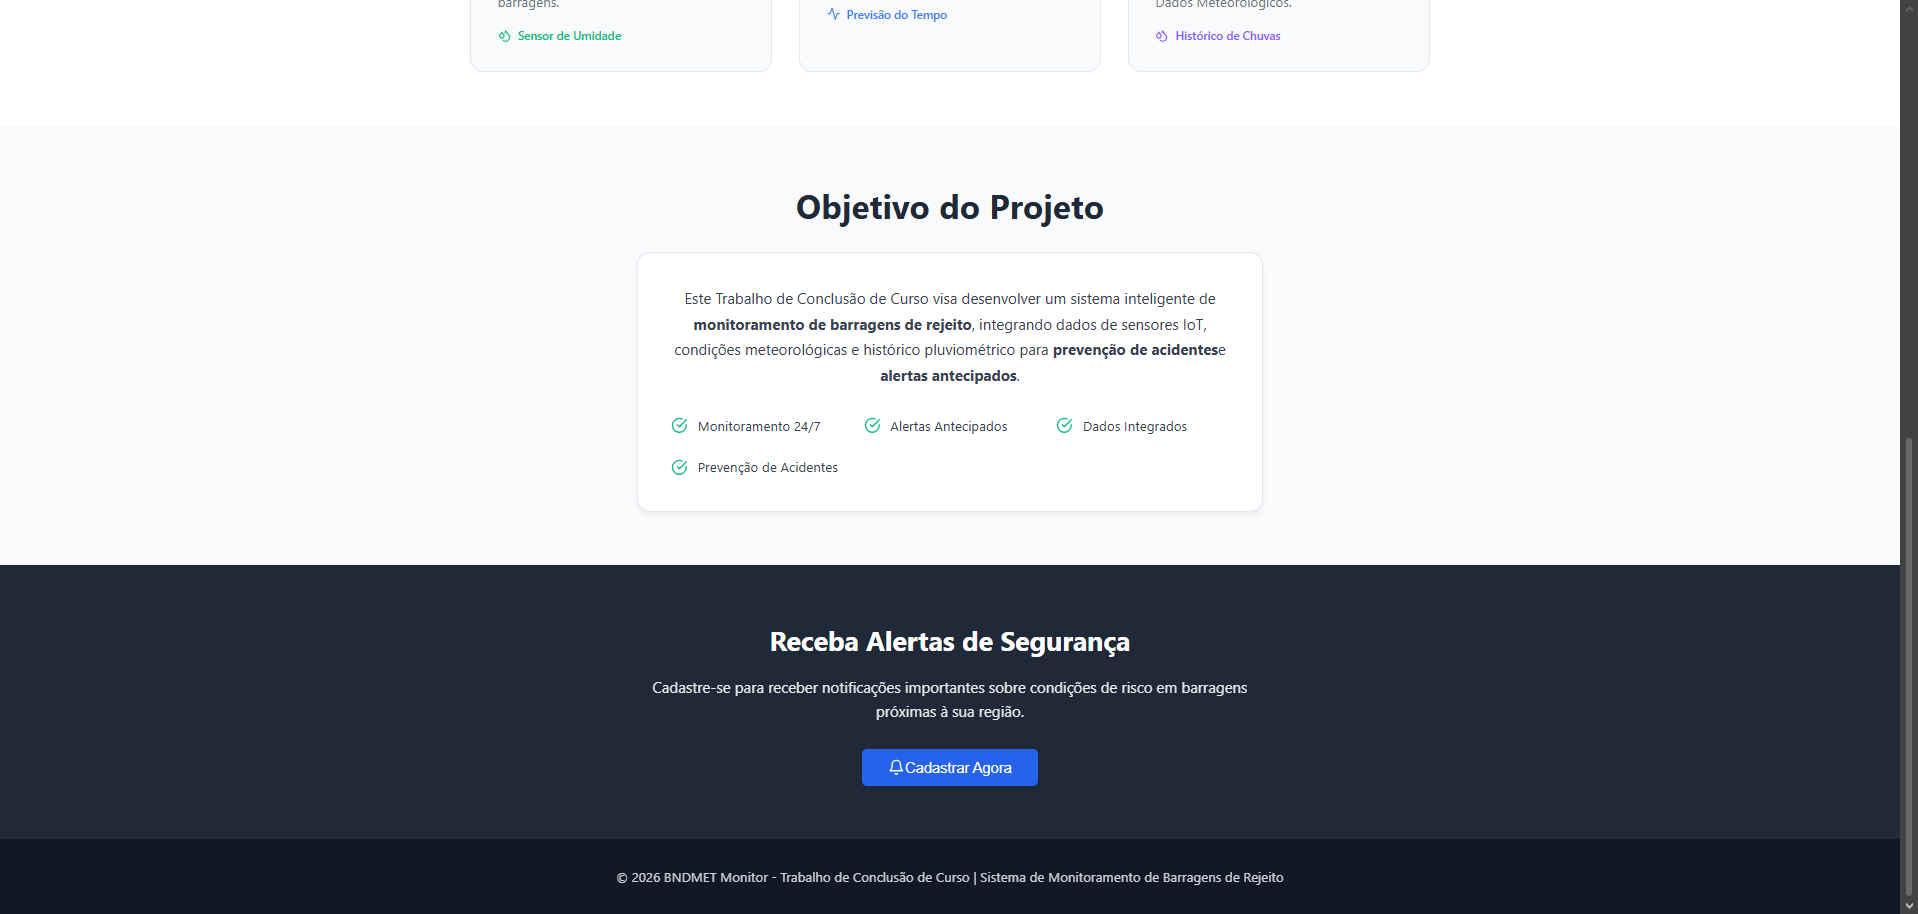
\includegraphics[width=0.95\textwidth]{figures/cap5_landing_page_pt2.png}
    \caption{\textit{Landing page} do sistema: apresentação das funcionalidades e botão de cadastro público.}
    \label{fig:landing_page_pt2}
    \fonte{Elaborado pela autora.}
\end{figure}

Ao clicar em ``Cadastrar para Receber Alertas'', um modal é exibido com
os campos nome, e-mail, telefone --- com máscara automática no formato
\texttt{(XX) XXXXX-XXXX} aplicada à medida que o usuário digita ---,
preferência de recebimento de notificações e tipo de notificação. Após
o preenchimento e confirmação, o sistema exibe o \textit{toast} ``Cadastro
realizado com sucesso! Você receberá notificações sobre os alertas de
barragem'' e o modal é fechado, conforme ilustra a \autoref{fig:cadastro_modal_preenchido_pt1} e a \autoref{fig:cadastro_modal_preenchido_pt2}.

\begin{figure}[htbp]
    \centering
    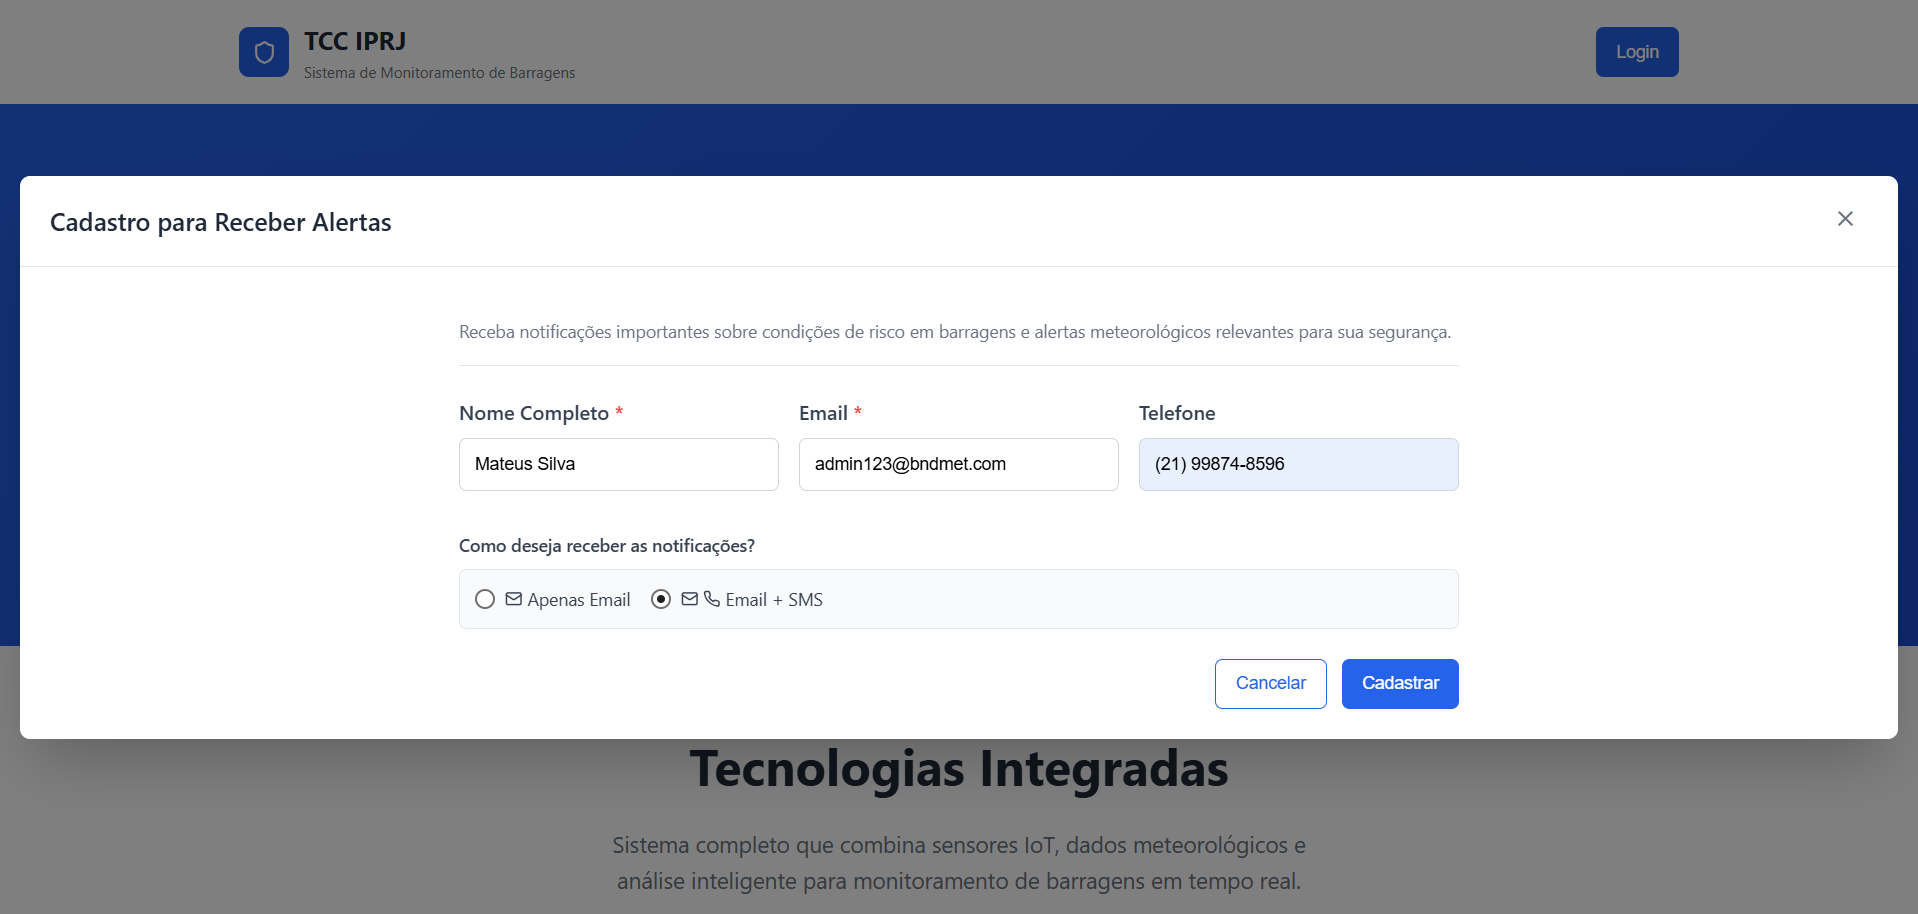
\includegraphics[width=0.75\textwidth]{figures/cap5_cadastro_modal_preenchido_pt1.png}
    \caption{Modal de cadastro para receber alertas com campos preenchidos: nome, e-mail, telefone com máscara automática e preferência de notificação.}
    \label{fig:cadastro_modal_preenchido_pt1}
    \fonte{Elaborado pela autora.}
\end{figure}

\begin{figure}[htbp]
    \centering
    
\includegraphics[width=0.75\textwidth]{figures/cap5_cadastro_modal_preenchido_pt2.png}
    \caption{\textit{toast} de confirmação exibido após envio bem-sucedido.}
    \label{fig:cadastro_modal_preenchido_pt2}
    \fonte{Elaborado pela autora.}
\end{figure}

Quando o e-mail informado já consta no cadastro, o \textit{backend}
retorna erro e o sistema exibe uma mensagem de alerta ao usuário,
mantendo o formulário aberto para correção, conforme ilustra a \autoref{fig:cadastro_email_duplicado}. 

\begin{figure}[htbp]
    \centering
    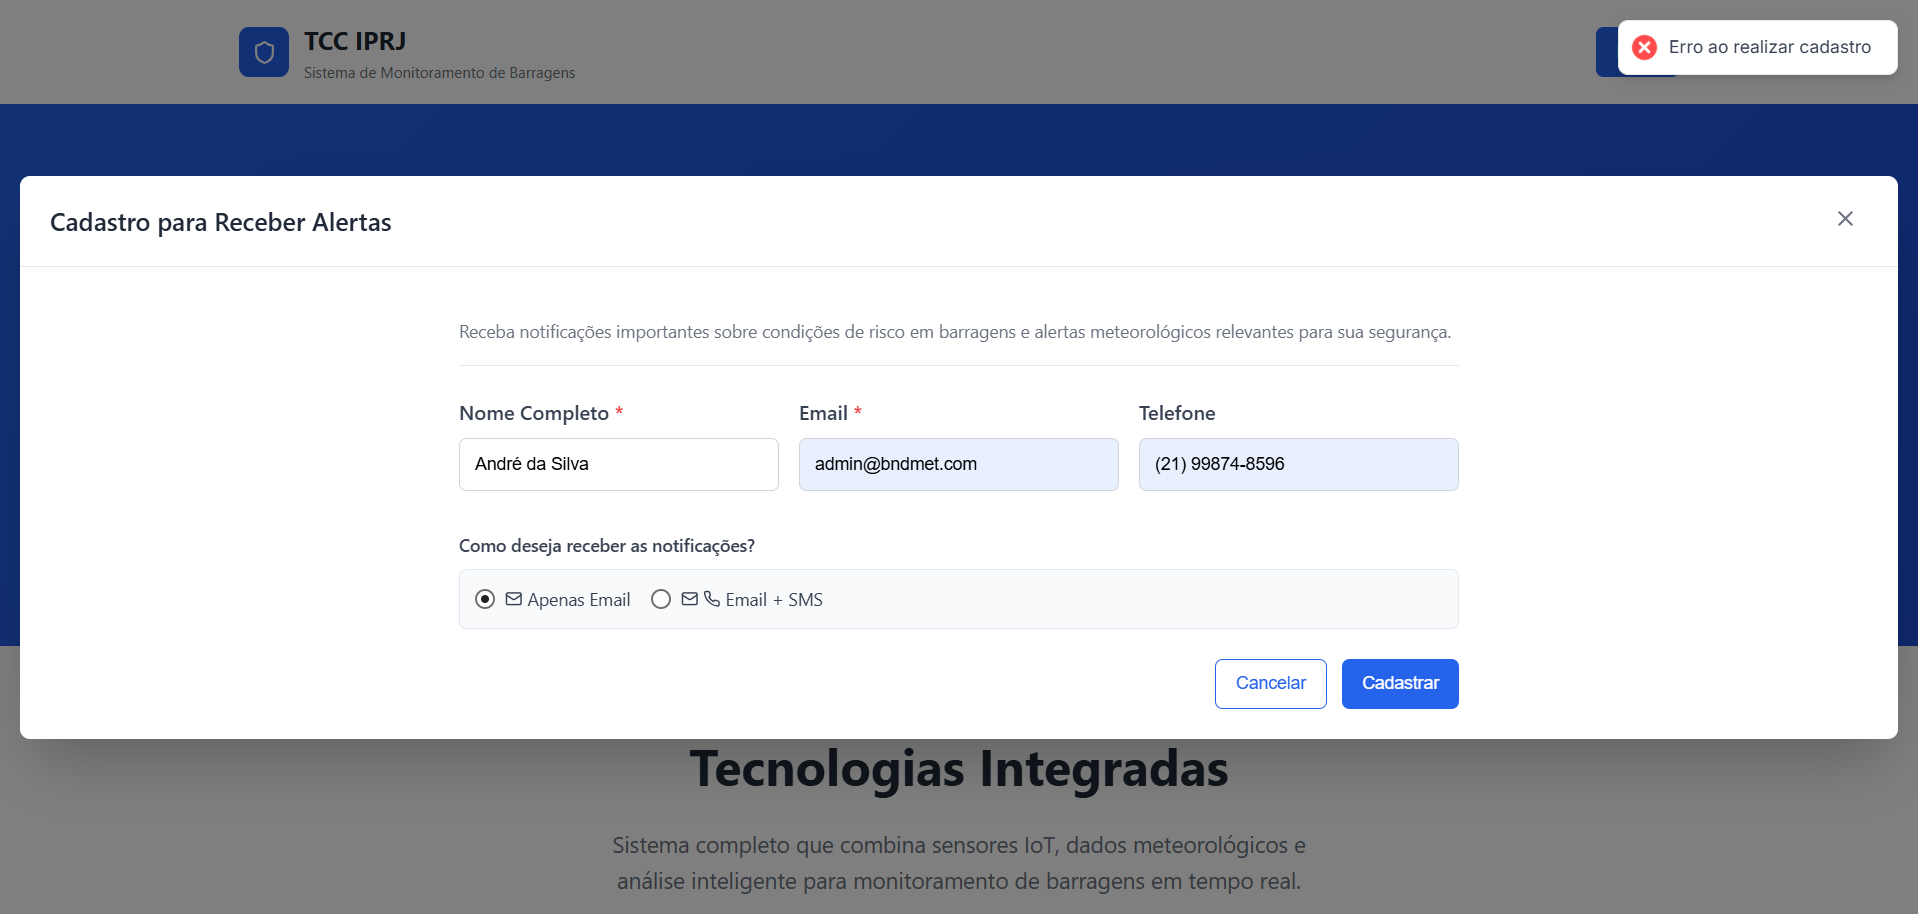
\includegraphics[width=0.75\textwidth]{figures/cap5_cadastro_email_duplicado.png}
    \caption{Modal de cadastro com \textit{toast} de erro retornado pelo \textit{backend}: e-mail já registrado no sistema; formulário mantido aberto para correção do dado.}
    \label{fig:cadastro_email_duplicado}
    \fonte{Elaborado pela autora.}
\end{figure}

Campos obrigatórios não preenchidos impedem o envio
e exibem mensagem de erro inline no próprio campo, conforme ilustra a \autoref{fig:cadastro_campos_vazios}.

\begin{figure}[htbp]
    \centering
    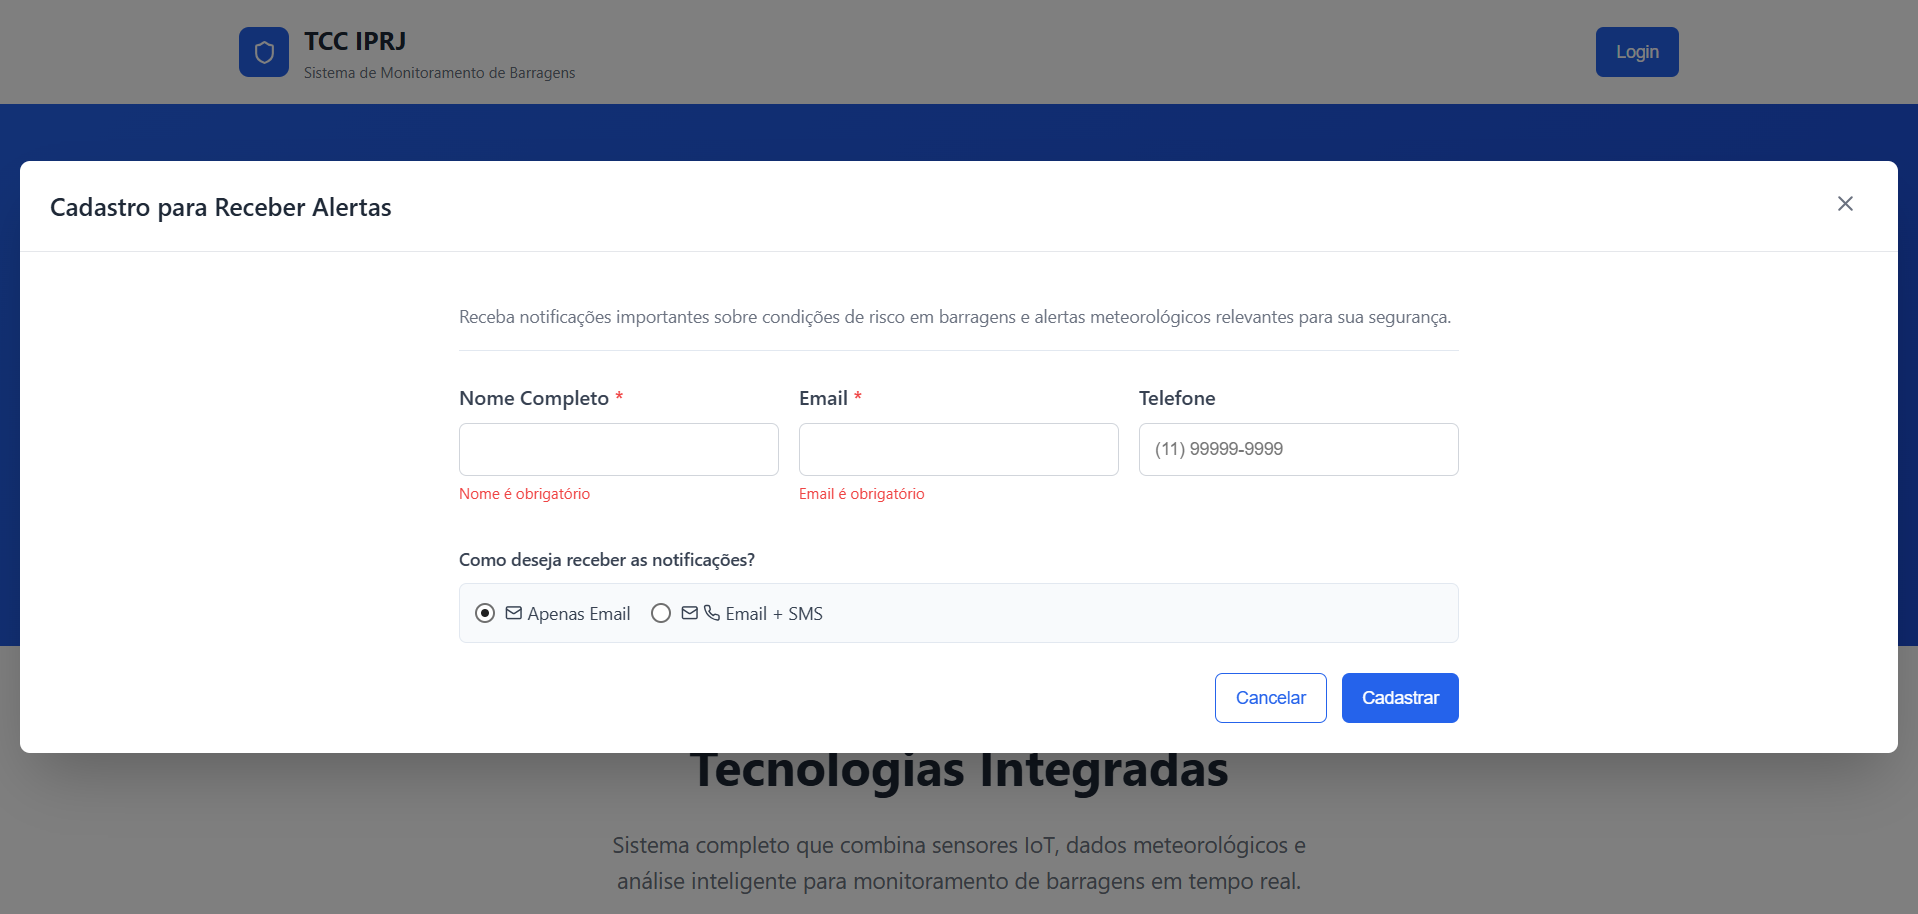
\includegraphics[width=0.75\textwidth]{figures/cap5_cadastro_campos_vazios.png}
    \caption{Modal de cadastro com validação de campos: mensagens de erro inline em campos obrigatórios não preenchidos.}
    \label{fig:cadastro_campos_vazios}
    \fonte{Elaborado pela autora.}
\end{figure}

Campos com formato inválido
--- como nome menor que 2 caracteres, e-mail sem o símbolo @, e telefone com menos de 11 dígitos, por exemplo --- também impedem o envio
e exibem mensagem de erro inline no próprio campo, conforme ilustra a \autoref{fig:cadastro_campos_invalidos}.

\begin{figure}[htbp]
    \centering
    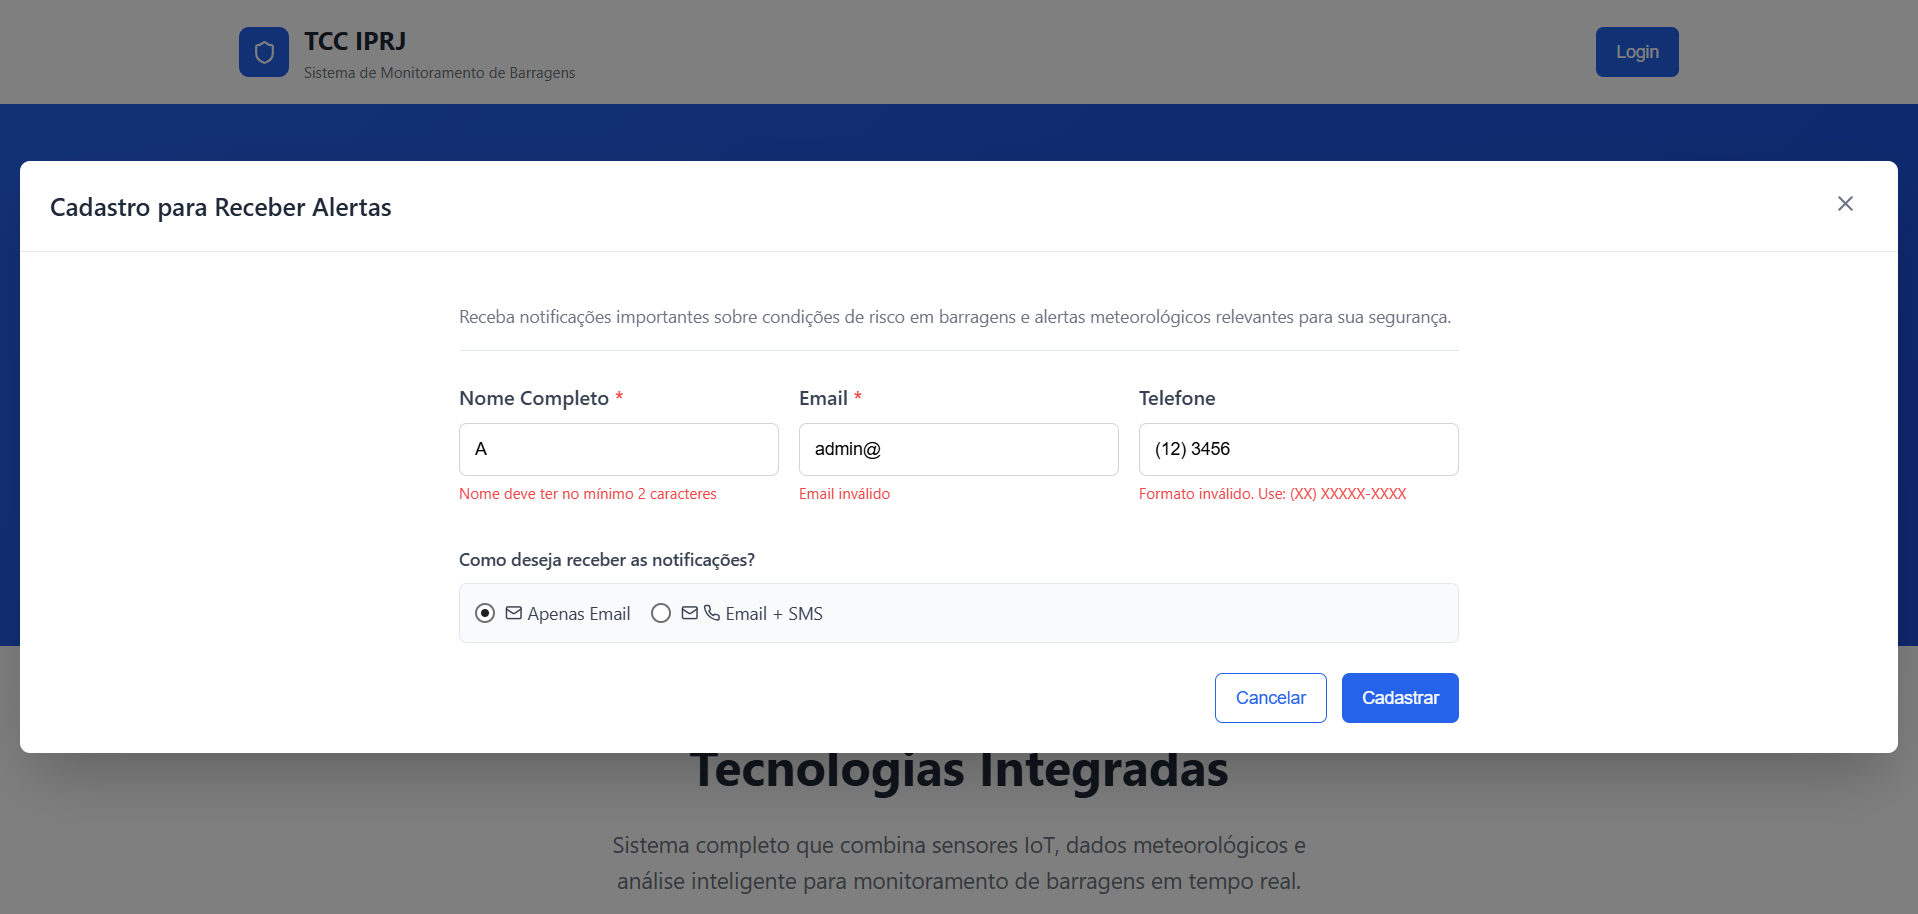
\includegraphics[width=0.75\textwidth]{figures/cap5_cadastro_campos_invalidos.png}
    \caption{Modal de cadastro com validação de campos: mensagens de erro inline em campos obrigatórios com formato inválido.}
    \label{fig:cadastro_campos_invalidos}
    \fonte{Elaborado pela autora.}
\end{figure}

% -------------------------------------------------------------
\subsection{Login}
\label{subsec:login}
% -------------------------------------------------------------

O acesso ao painel administrativo é feito por e-mail e senha na tela
de \textit{login} exibida na \autoref{fig:tela_login}. Ao confirmar as
credenciais, o sistema autentica o administrador, armazena o token de
sessão e o redireciona imediatamente para o \textit{dashboard}.

\begin{figure}[htbp]
    \centering
    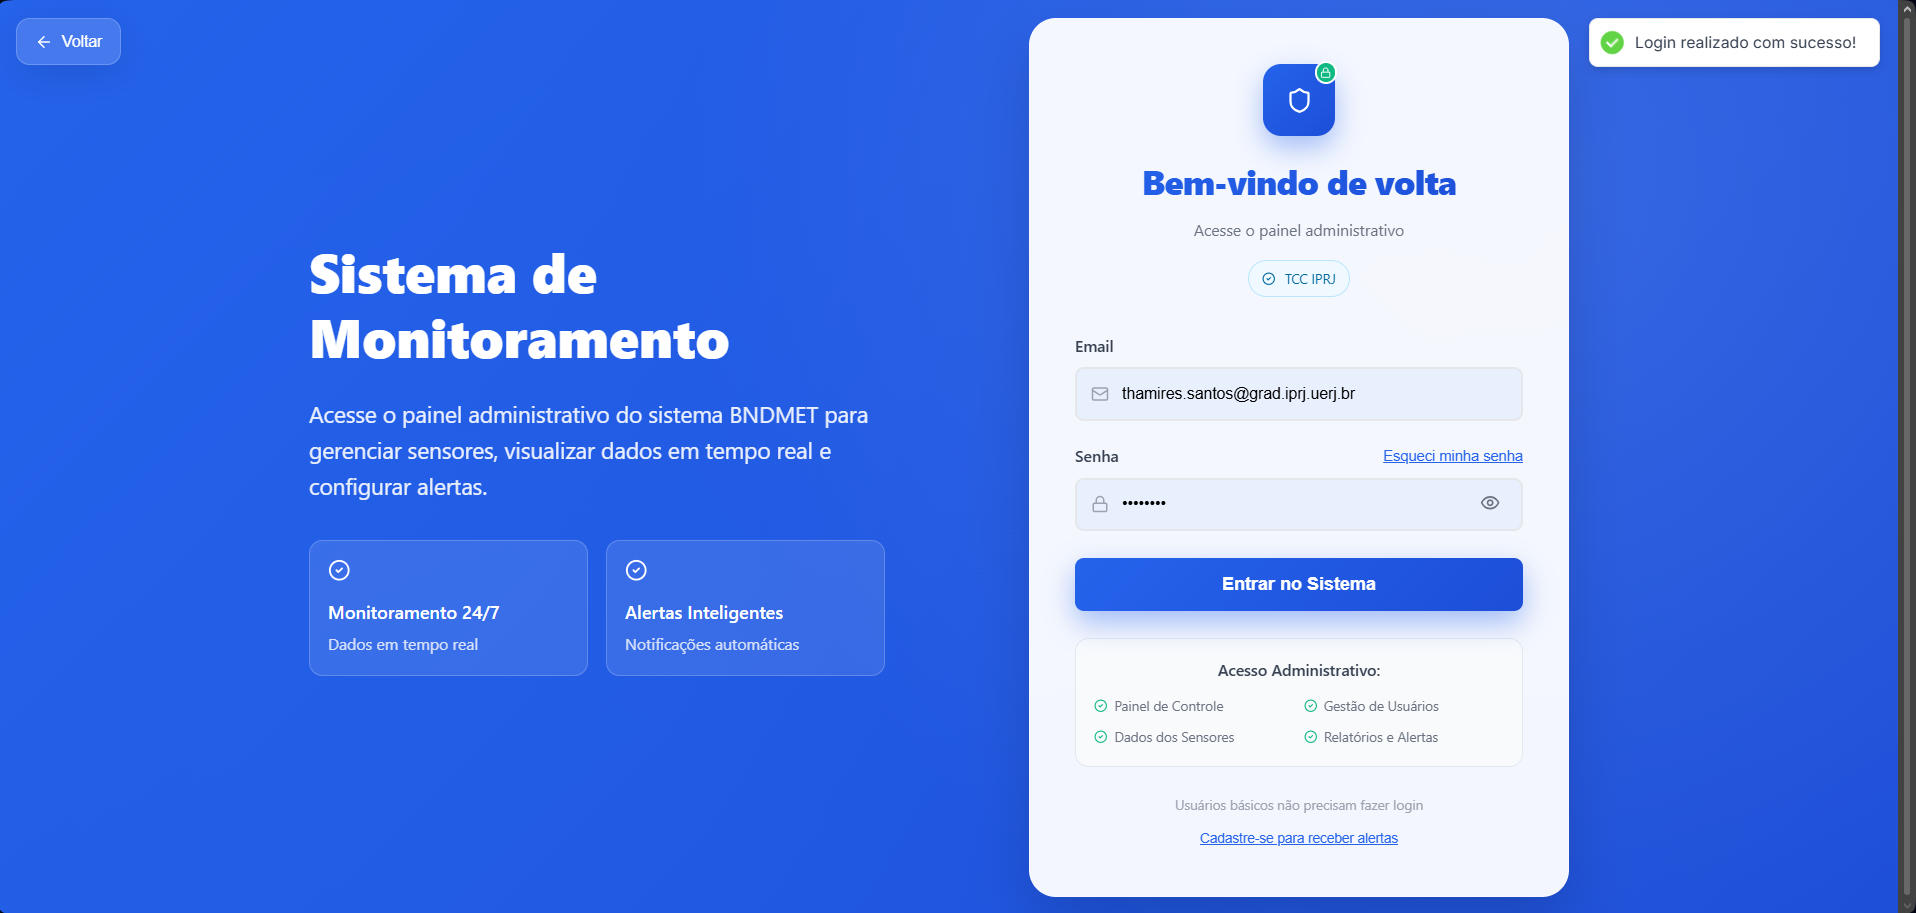
\includegraphics[width=0.75\textwidth]{figures/cap5_login.png}
    \caption{Tela de \textit{login}: campos de e-mail e senha com
    \textit{link} para recuperação de senha e botão de acesso.}
    \label{fig:tela_login}
    \fonte{Elaborado pela autora.}
\end{figure}

Quando as credenciais são inválidas --- seja por senha incorreta ou por
e-mail inexistente --- o \textit{backend} retorna a mensagem ``Credenciais
inválidas'' sem especificar qual campo está errado, preservando a
segurança do sistema, conforme ilustra a \autoref{fig:login_erro_credenciais}. O mesmo comportamento se aplica a contas
desativadas: a mensagem genérica não revela que a conta existe mas
está inativa.

\begin{figure}[htbp]
    \centering
    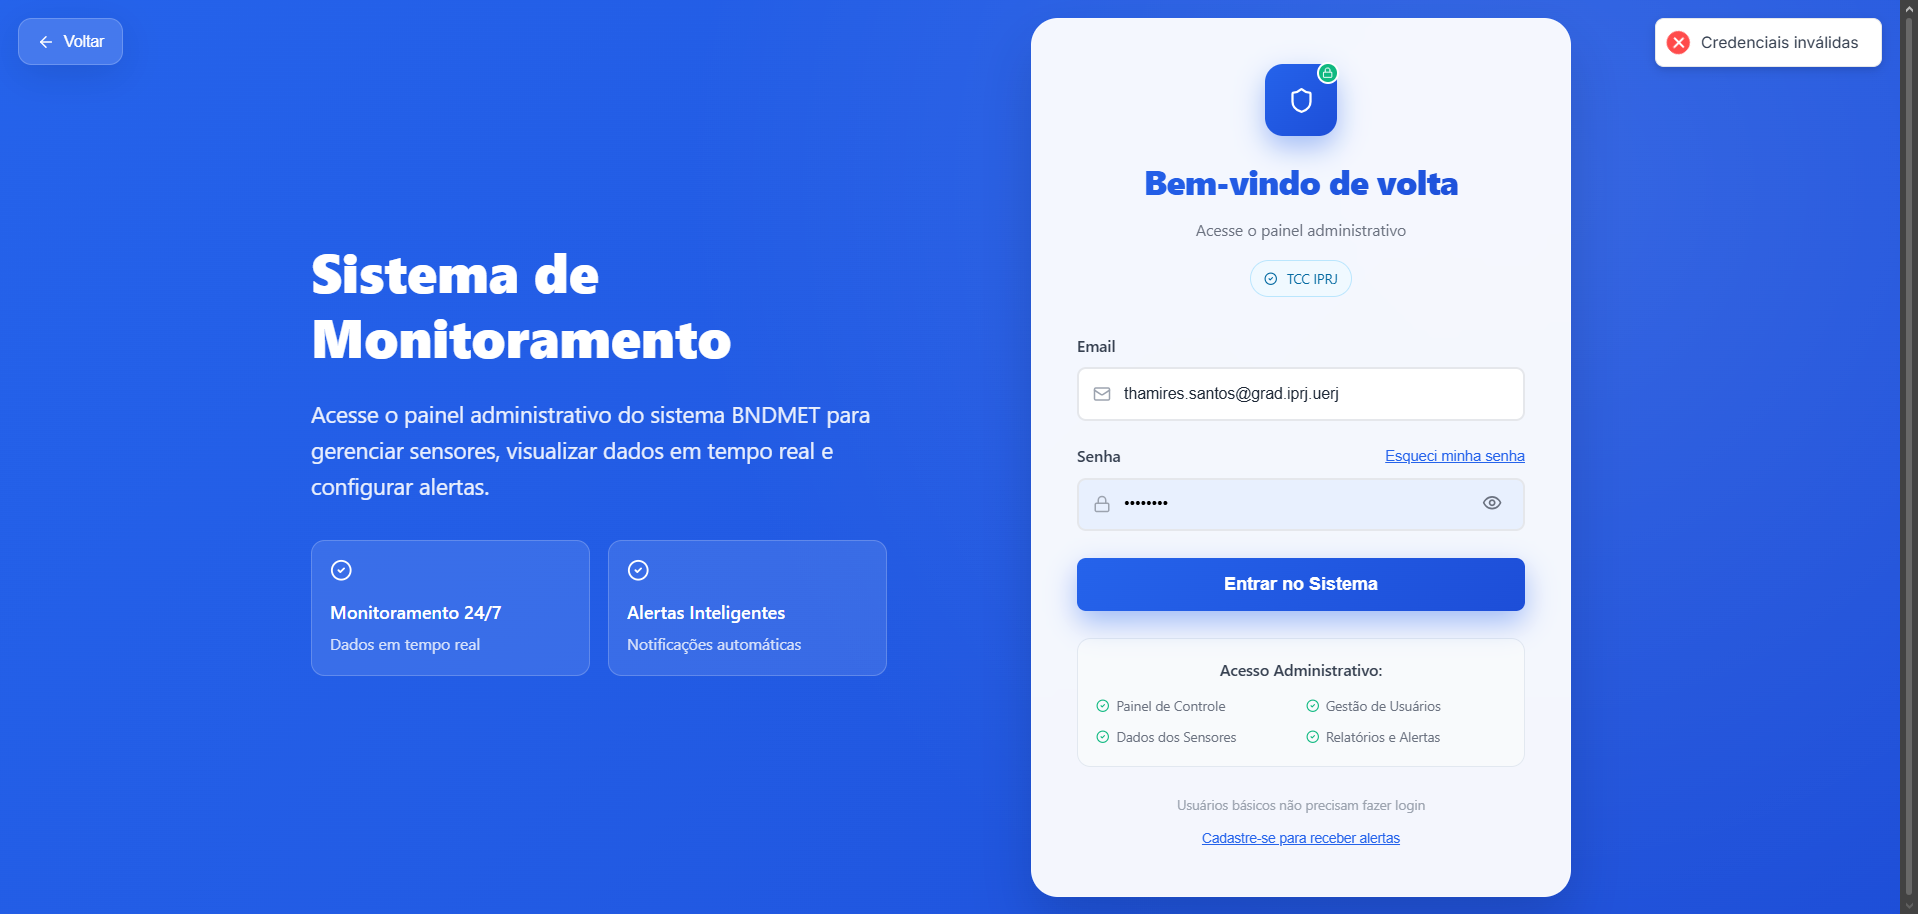
\includegraphics[width=0.75\textwidth]{figures/cap5_login_erro_credenciais.png}
    \caption{Tela de \textit{login} com mensagem de credenciais inválidas: resposta genérica ``Credenciais inválidas'' sem indicar qual campo está incorreto, preservando a segurança da conta.}
    \label{fig:login_erro_credenciais}
    \fonte{Elaborado pela autora.}
\end{figure}

Se o token de sessão expirar durante o uso do sistema, o
\textit{middleware} de autenticação rejeita a próxima requisição, o
\textit{frontend} remove os dados de sessão armazenados e redireciona
o usuário à tela de \textit{login}, conforme demonstram as
\autoref{fig:login_sessao_expirada_pt1},
\autoref{fig:login_sessao_expirada_pt2} e
\autoref{fig:login_sessao_expirada_pt3}.

\begin{figure}[htbp]
    \centering
    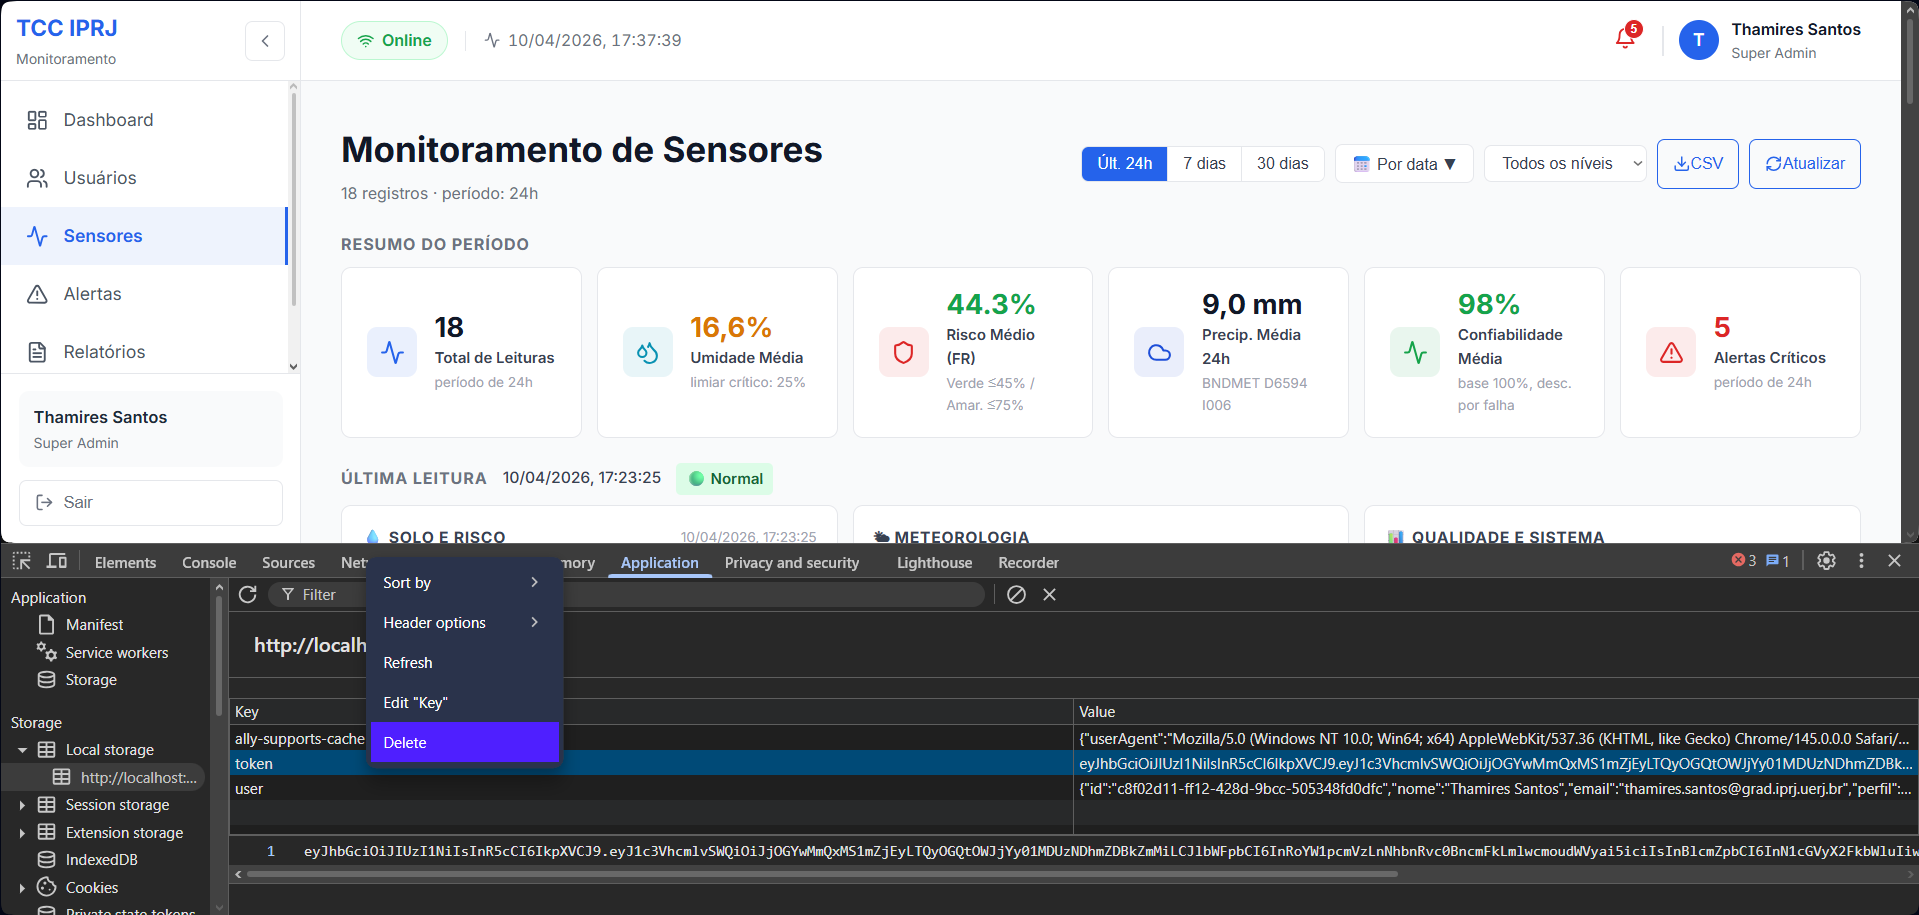
\includegraphics[width=0.75\textwidth]{figures/cap5_login_sessao_expirada_pt1.png}
    \caption{Sessão expirada (parte~1): dados de sessão locais removidos
    pelo \textit{frontend} após rejeição do token.}
    \label{fig:login_sessao_expirada_pt1}
    \fonte{Elaborado pela autora.}
\end{figure}

\begin{figure}[htbp]
    \centering
    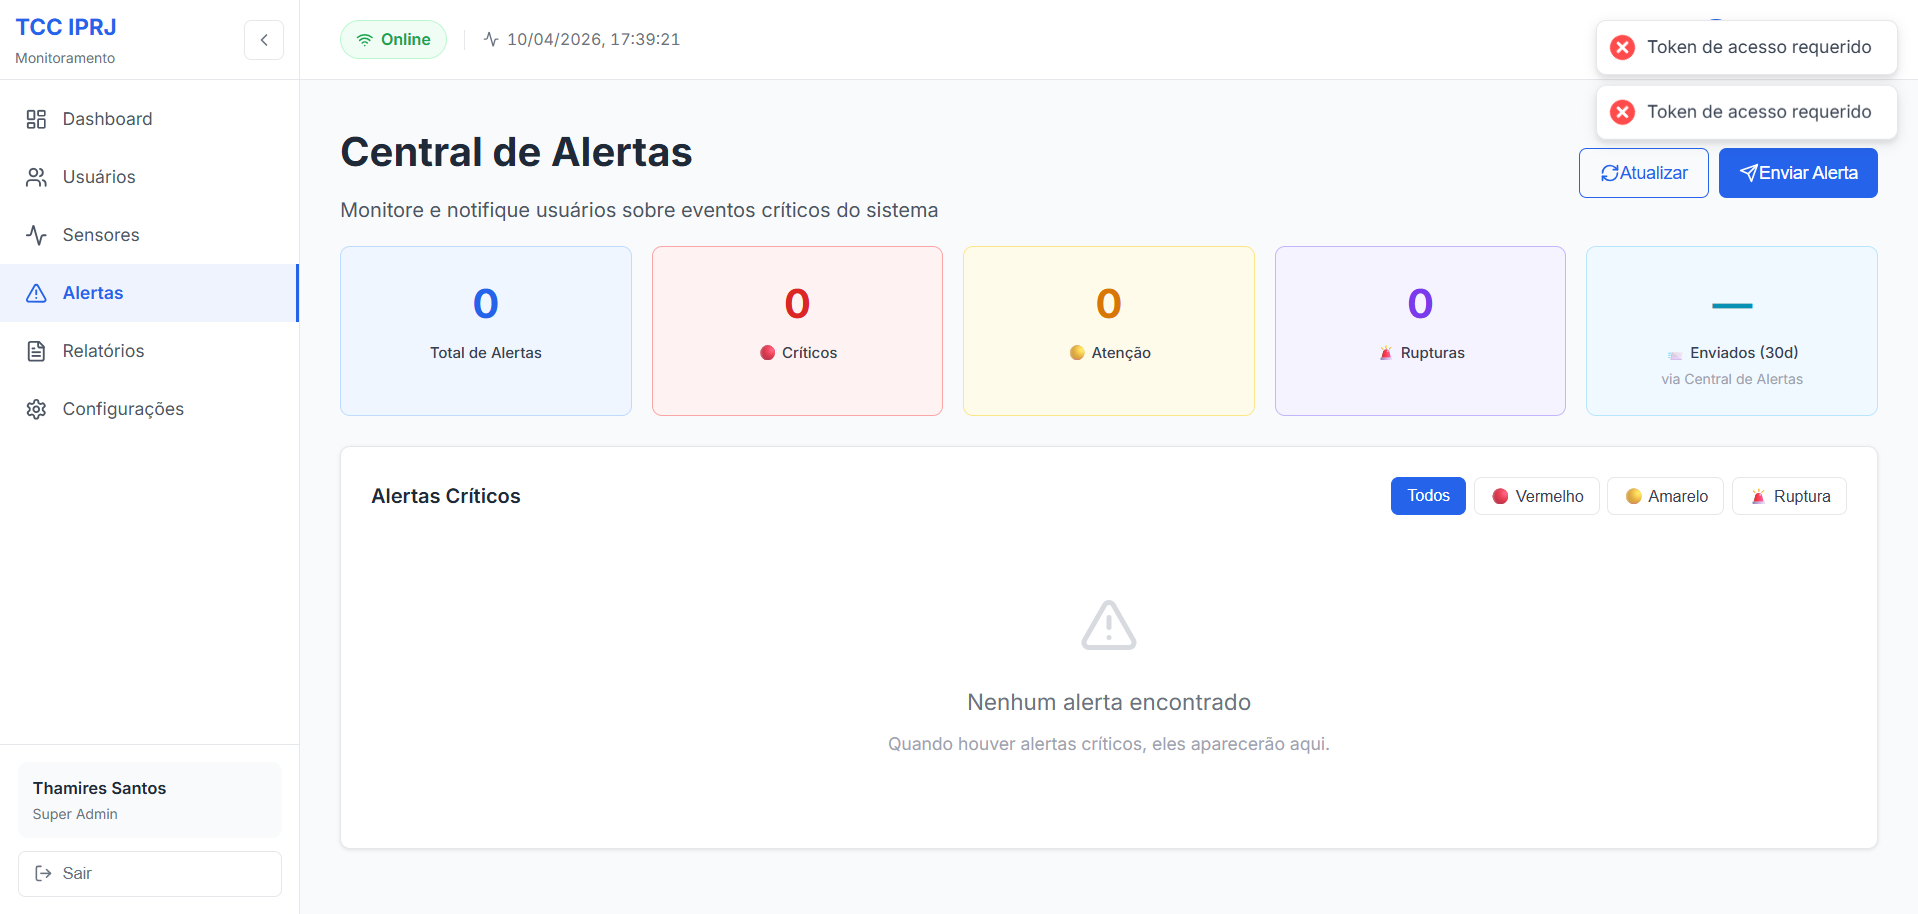
\includegraphics[width=0.75\textwidth]{figures/cap5_login_sessao_expirada_pt2.png}
    \caption{Sessão expirada (parte~2): token rejeitado pelo
    \textit{middleware} de autenticação na próxima requisição.}
    \label{fig:login_sessao_expirada_pt2}
    \fonte{Elaborado pela autora.}
\end{figure}

\begin{figure}[htbp]
    \centering
    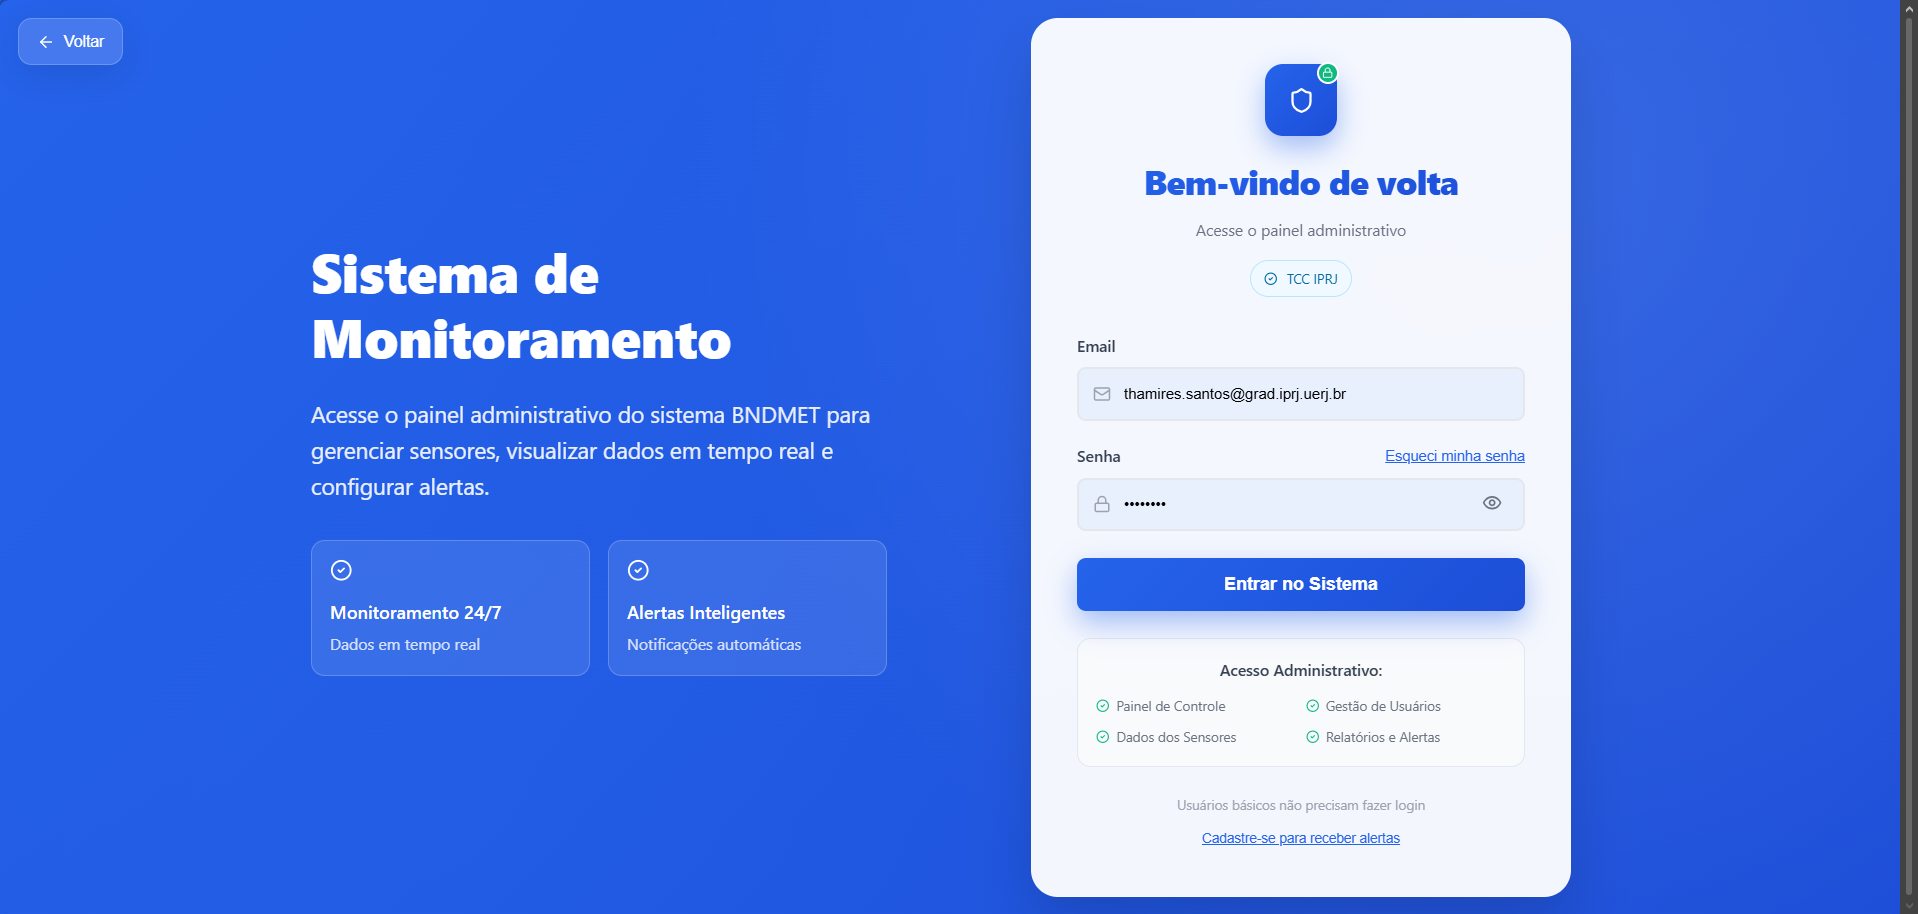
\includegraphics[width=0.75\textwidth]{figures/cap5_login_sessao_expirada_pt3.png}
    \caption{Sessão expirada (parte~3): tela de \textit{login} exibida
    após redirecionamento automático; administrador retorna ao fluxo de
    autenticação sem ação manual.}
    \label{fig:login_sessao_expirada_pt3}
    \fonte{Elaborado pela autora.}
\end{figure}

% -------------------------------------------------------------
\subsection{Logout}
\label{subsec:logout}
% -------------------------------------------------------------

O \textit{logout} é realizado pelo botão ``Sair'' disponível no menu
lateral. Ao clicar, a sessão é invalidada no servidor, os dados locais
são removidos e o administrador é redirecionado para a tela de
\textit{login} com o \textit{toast} ``Logout realizado com sucesso!''.
Mesmo que ocorra um erro na chamada ao \textit{backend} durante o
\textit{logout}, o \textit{frontend} remove os dados locais e realiza o
redirecionamento de qualquer forma, garantindo que o administrador não
permaneça preso no sistema, conforme ilustra a \autoref{fig:logout_redirecionamento}.

\begin{figure}[htbp]
    \centering
    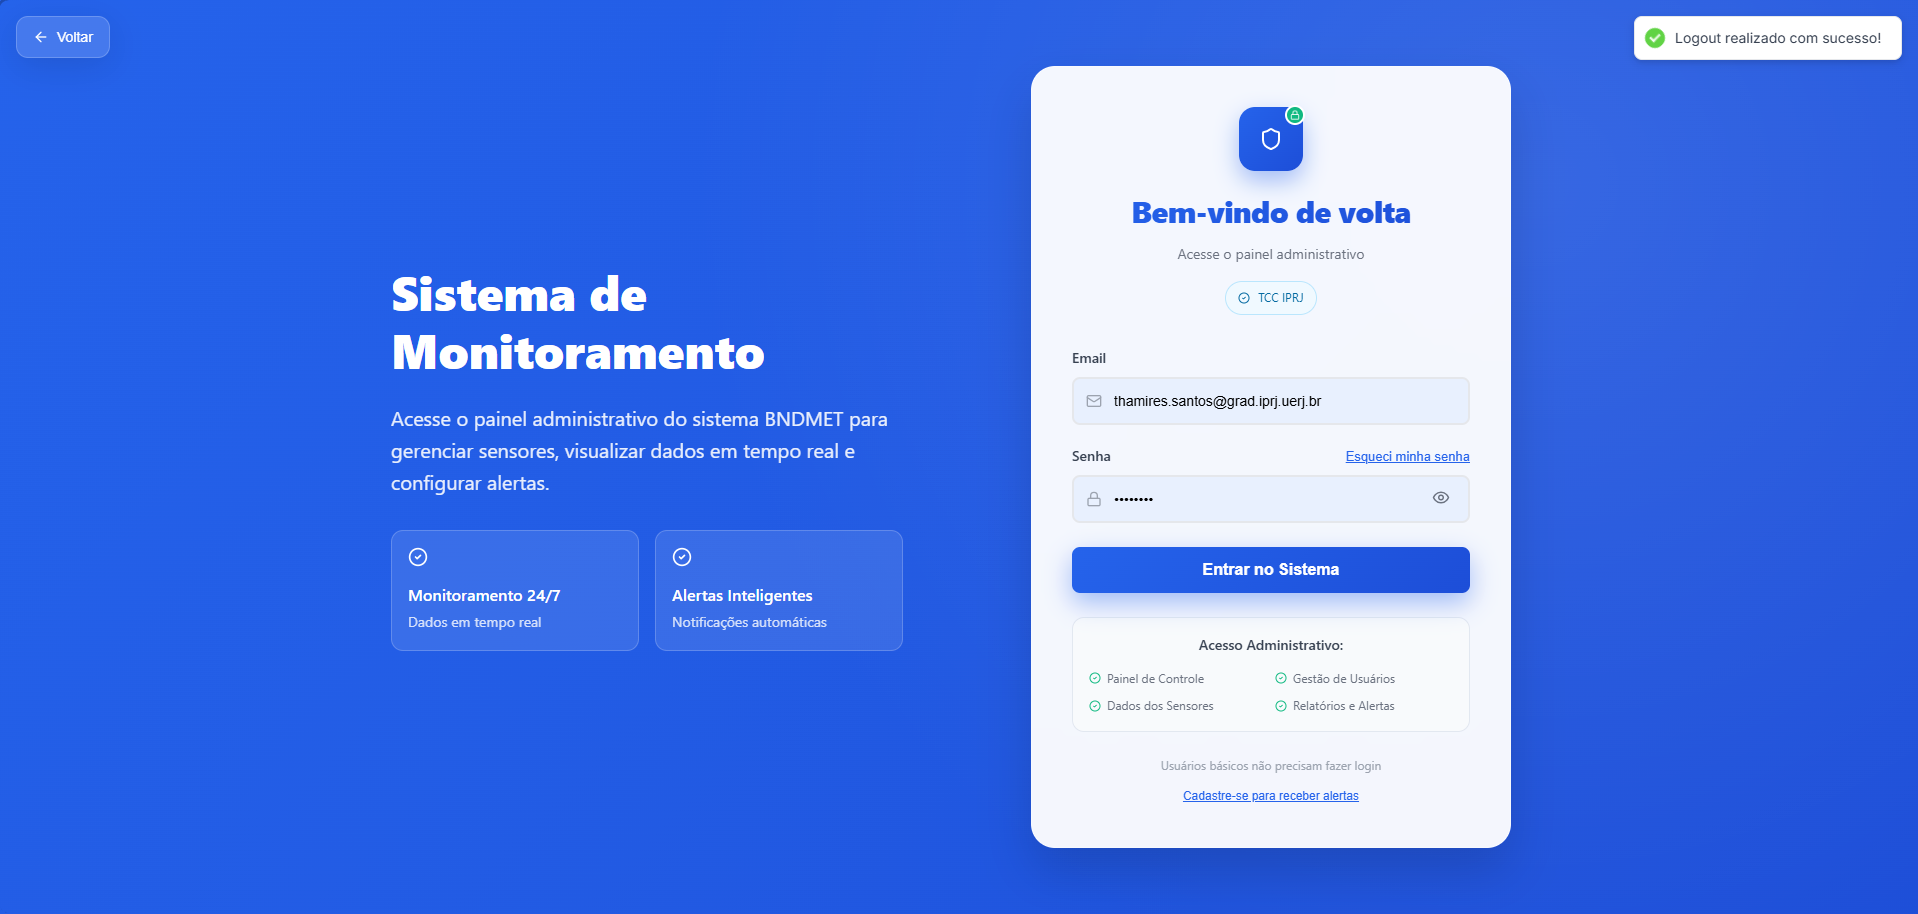
\includegraphics[width=0.75\textwidth]{figures/cap5_logout_redirecionamento.png}
    \caption{Tela de \textit{login} exibida após \textit{logout}: sessão encerrada no servidor, dados locais removidos e administrador redirecionado automaticamente; comportamento idêntico em caso de erro silencioso na chamada ao \textit{backend}.}
    \label{fig:logout_redirecionamento}
    \fonte{Elaborado pela autora.}
\end{figure}

% -------------------------------------------------------------
\subsection{Recuperação de Senha}
\label{subsec:reset-senha}
% -------------------------------------------------------------

A recuperação de senha é acessada pelo \textit{link} ``Esqueci minha
senha'' na tela de \textit{login}. O administrador informa seu e-mail
cadastrado e o sistema exibe uma resposta genérica --- sem indicar se
o endereço existe ou não --- para não expor informações sobre as contas
cadastradas, conforme demonstram as \autoref{fig:reset_solicitar_email_pt1} e \autoref{fig:reset_solicitar_email_pt2}.

\begin{figure}[htbp]
    \centering
    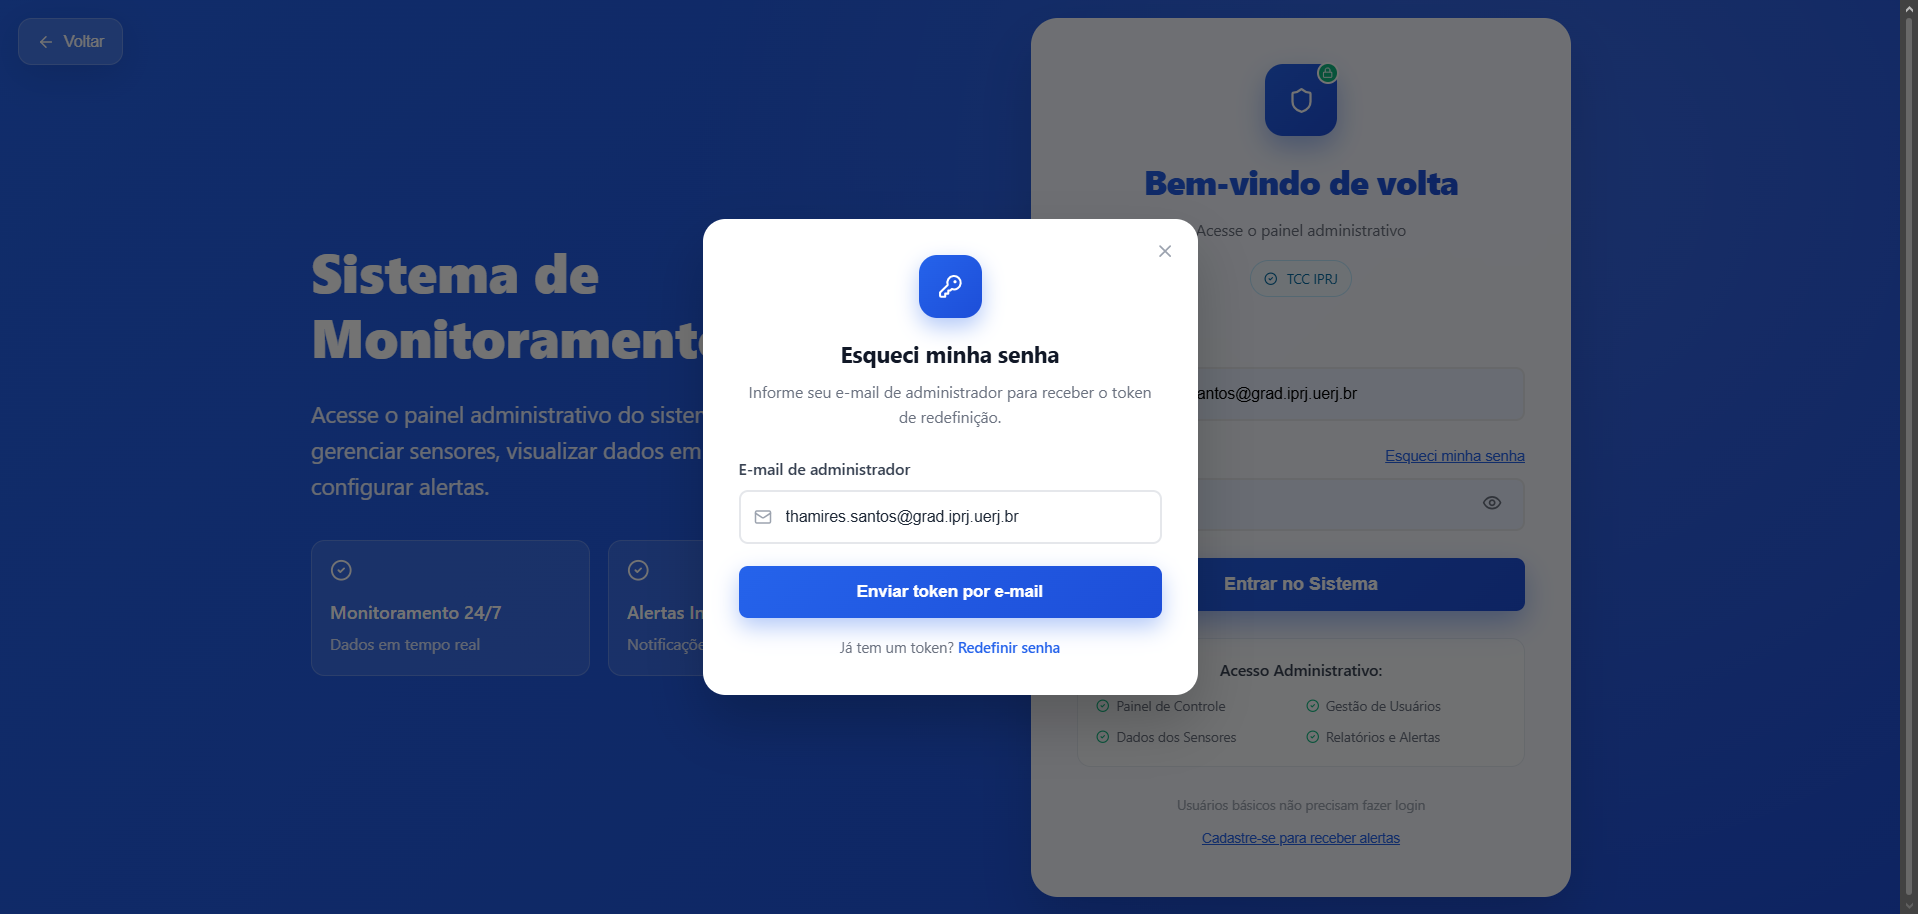
\includegraphics[width=0.75\textwidth]{figures/cap5_reset_solicitar_email_pt1.png}
    \caption{Tela de solicitação de recuperação de senha: campo de e-mail preenchido.}
    \label{fig:reset_solicitar_email_pt1}
    \fonte{Elaborado pela autora.}
\end{figure}

\begin{figure}[htbp]
    \centering
    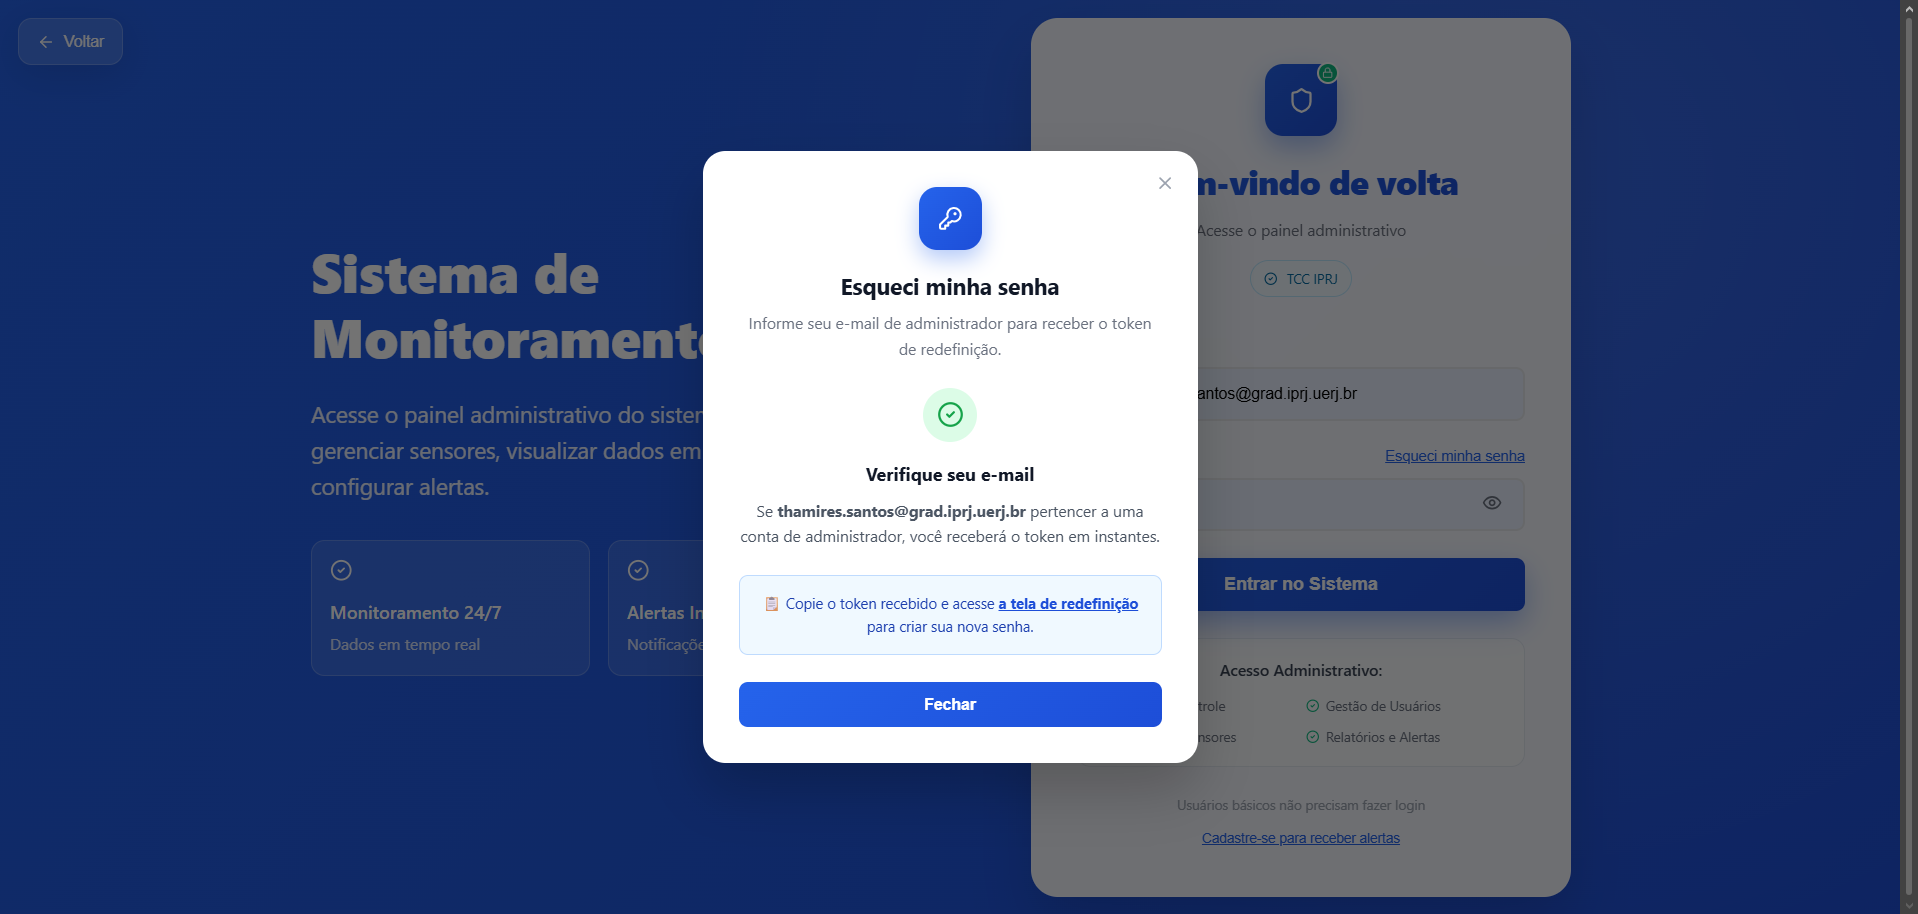
\includegraphics[width=0.75\textwidth]{figures/cap5_reset_solicitar_email_pt2.png}
    \caption{Tela de solicitação de recuperação de senha: resposta genérica exibida pelo sistema independente de o endereço existir ou não na base de dados.}
    \label{fig:reset_solicitar_email_pt2}
    \fonte{Elaborado pela autora.}
\end{figure}

Tentativas de recuperação de senha para e-mails de usuários básicos ---
que não possuem acesso administrativo --- recebem a mesma resposta
genérica, sem gerar token ou enviar e-mail, conforme ilustram as \autoref{fig:reset_usuario_basico_pt1} e \autoref{fig:reset_usuario_basico_pt2}.

\begin{figure}[htbp]
    \centering
    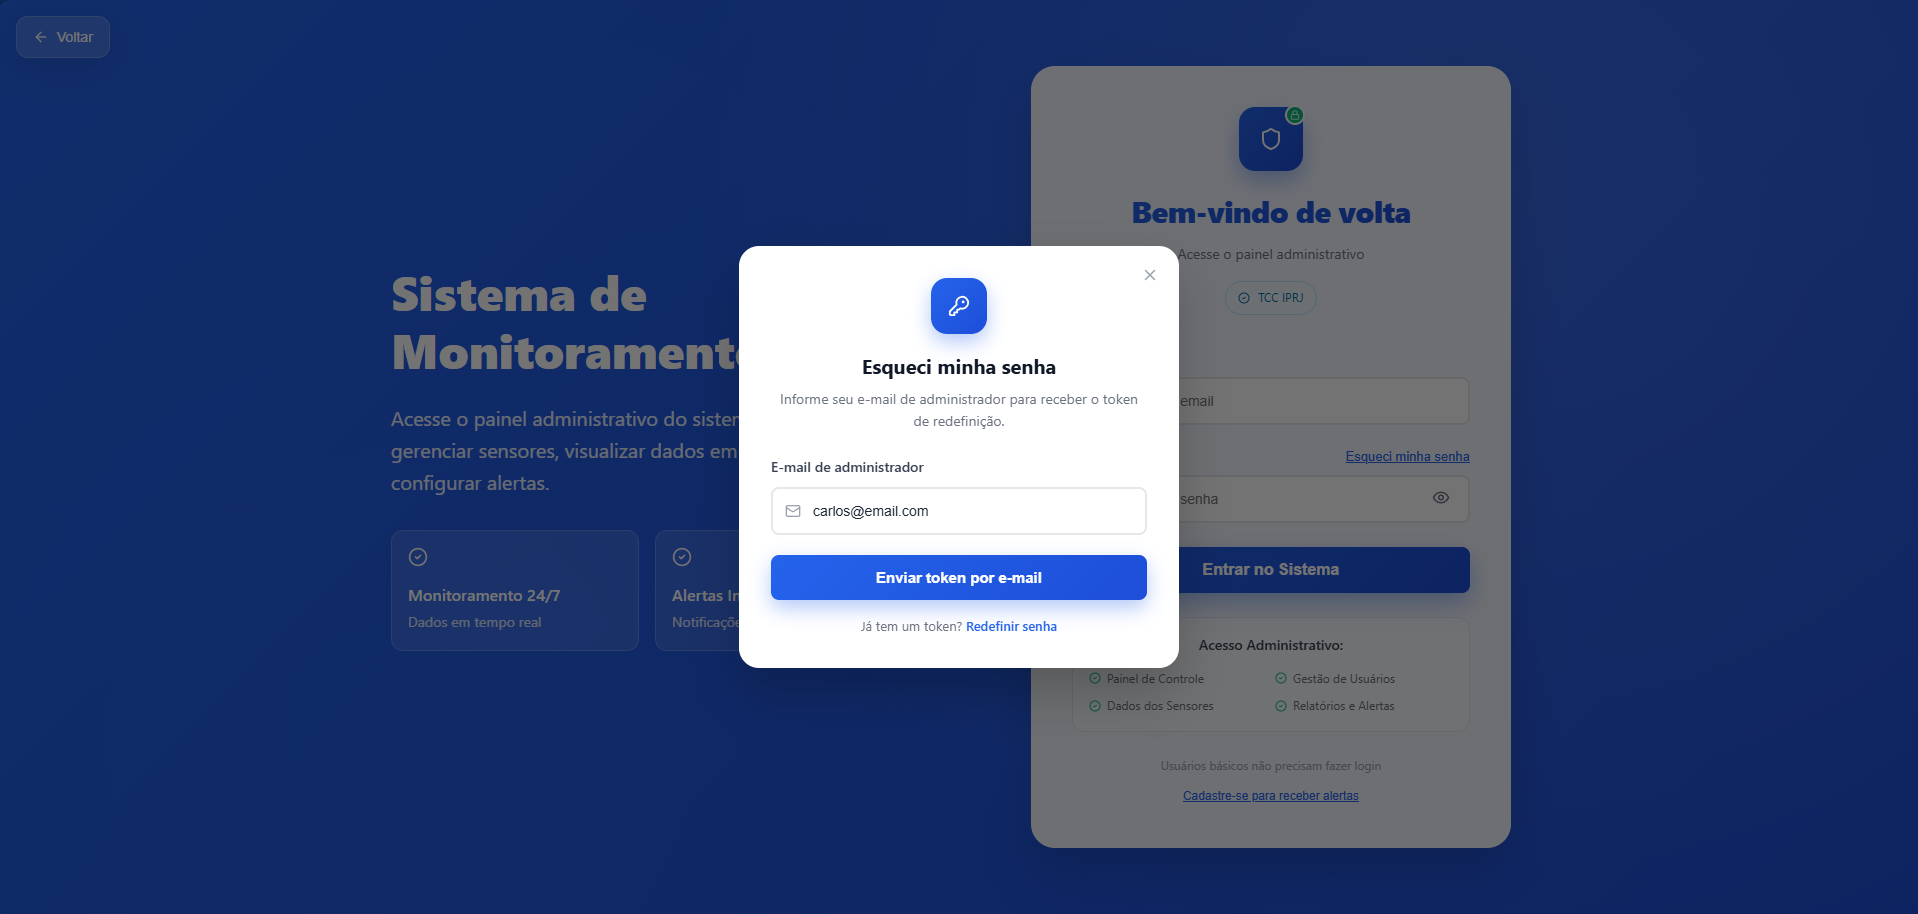
\includegraphics[width=0.75\textwidth]{figures/cap5_reset_usuario_basico_pt1.png}
    \caption{Tela de solicitação de recuperação de senha: campo de e-mail preenchido com e-mail de usuário básico.}
    \label{fig:reset_usuario_basico_pt1}
    \fonte{Elaborado pela autora.}
\end{figure}

\begin{figure}[htbp]
    \centering
    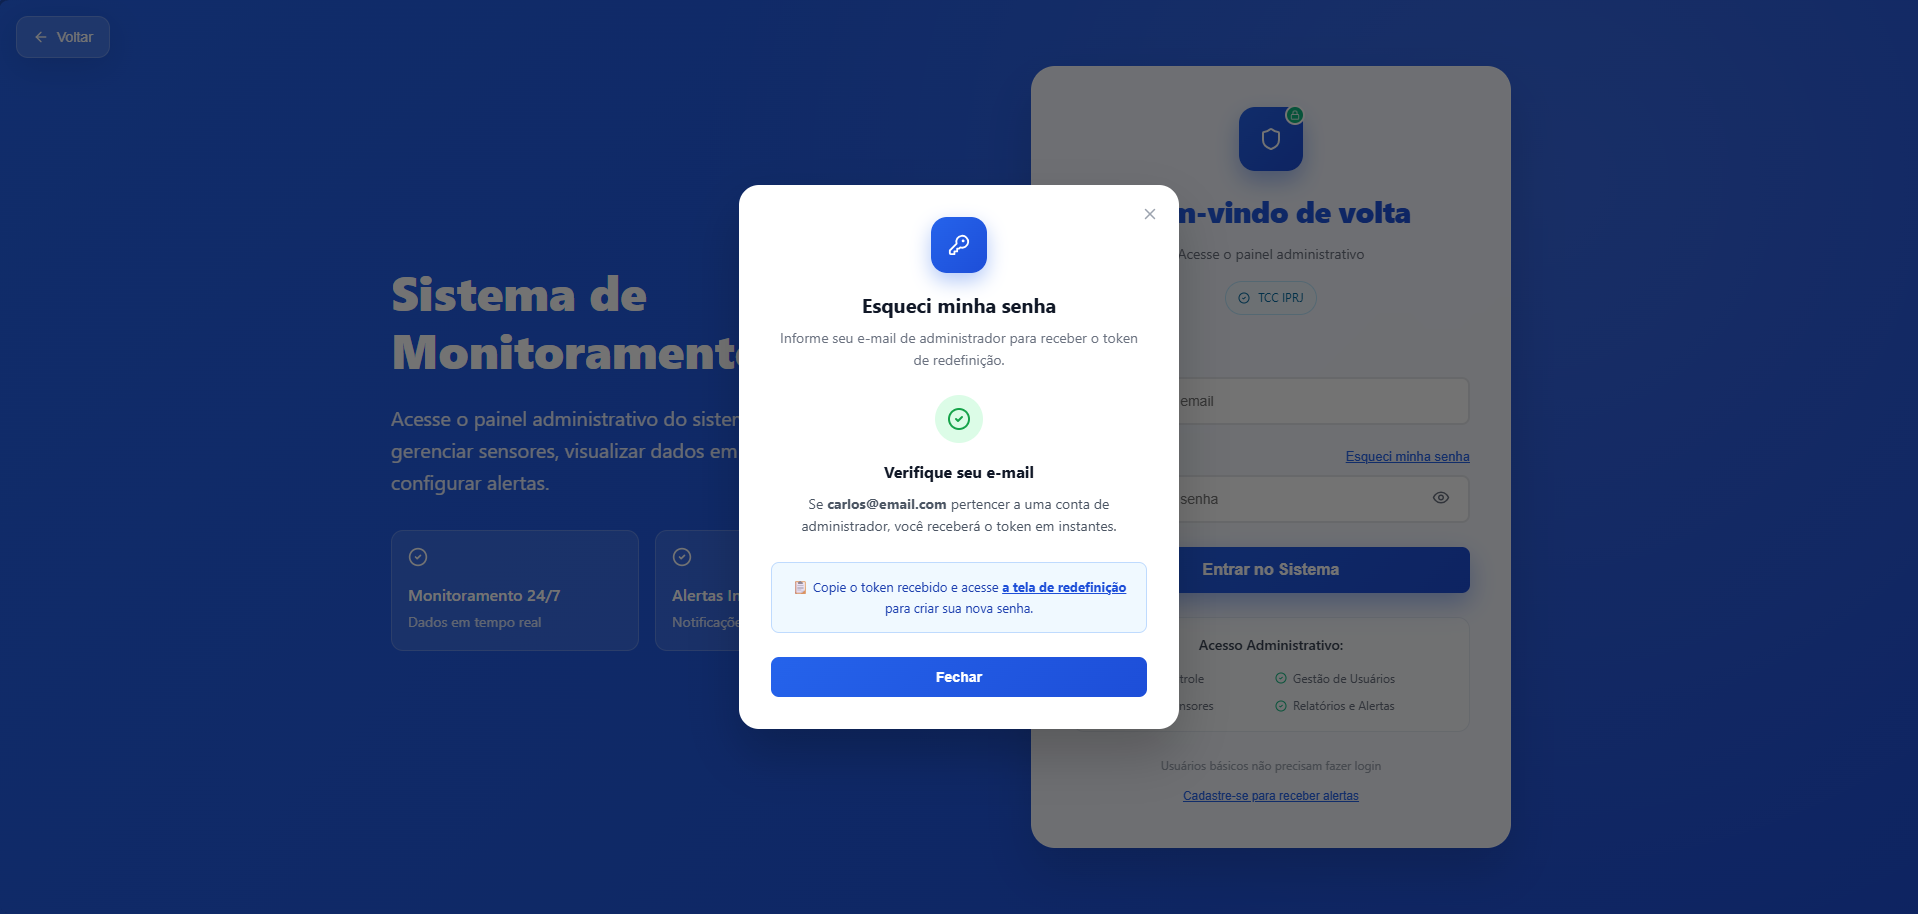
\includegraphics[width=0.75\textwidth]{figures/cap5_reset_usuario_basico_pt2.png}
    \caption{Tela de solicitação de recuperação de senha: resposta genérica exibida pelo sistema independente de o endereço existir ou não na base de dados.}
    \label{fig:reset_usuario_basico_pt2}
    \fonte{Elaborado pela autora.}
\end{figure}

Quando o e-mail é válido e pertence a um administrador
ativo, um token de redefinição é gerado e enviado por e-mail com
validade de 2 horas, acompanhado das instruções para utilizá-lo, conforme ilustram as \autoref{fig:reset_email_recebido_pt1} e \autoref{fig:reset_email_recebido_pt2}.

\begin{figure}[htbp]
    \centering
    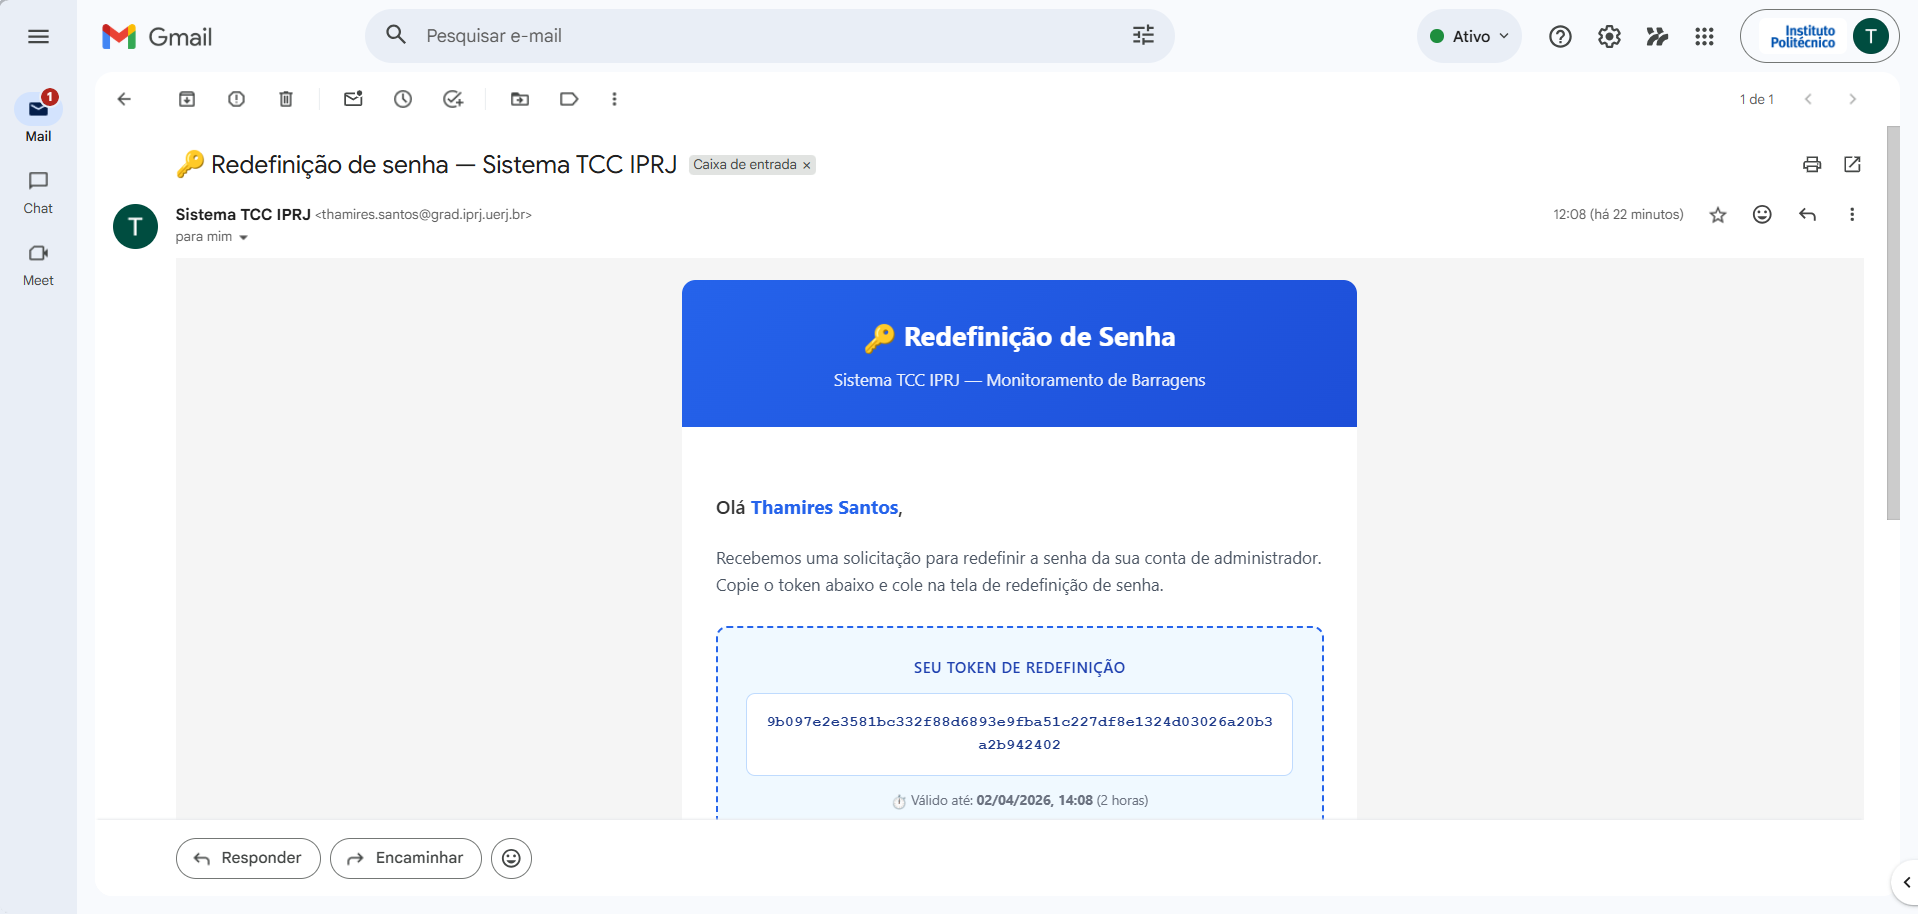
\includegraphics[width=0.75\textwidth]{figures/cap5_reset_email_recebido_pt1.png}
    \caption{Caixa de email com o token de recuperação de senha: o administrador ativo recebe por email o token de 64 caracteres.}
    \label{fig:reset_email_recebido_pt1}
    \fonte{Elaborado pela autora.}
\end{figure}

\begin{figure}[htbp]
    \centering
    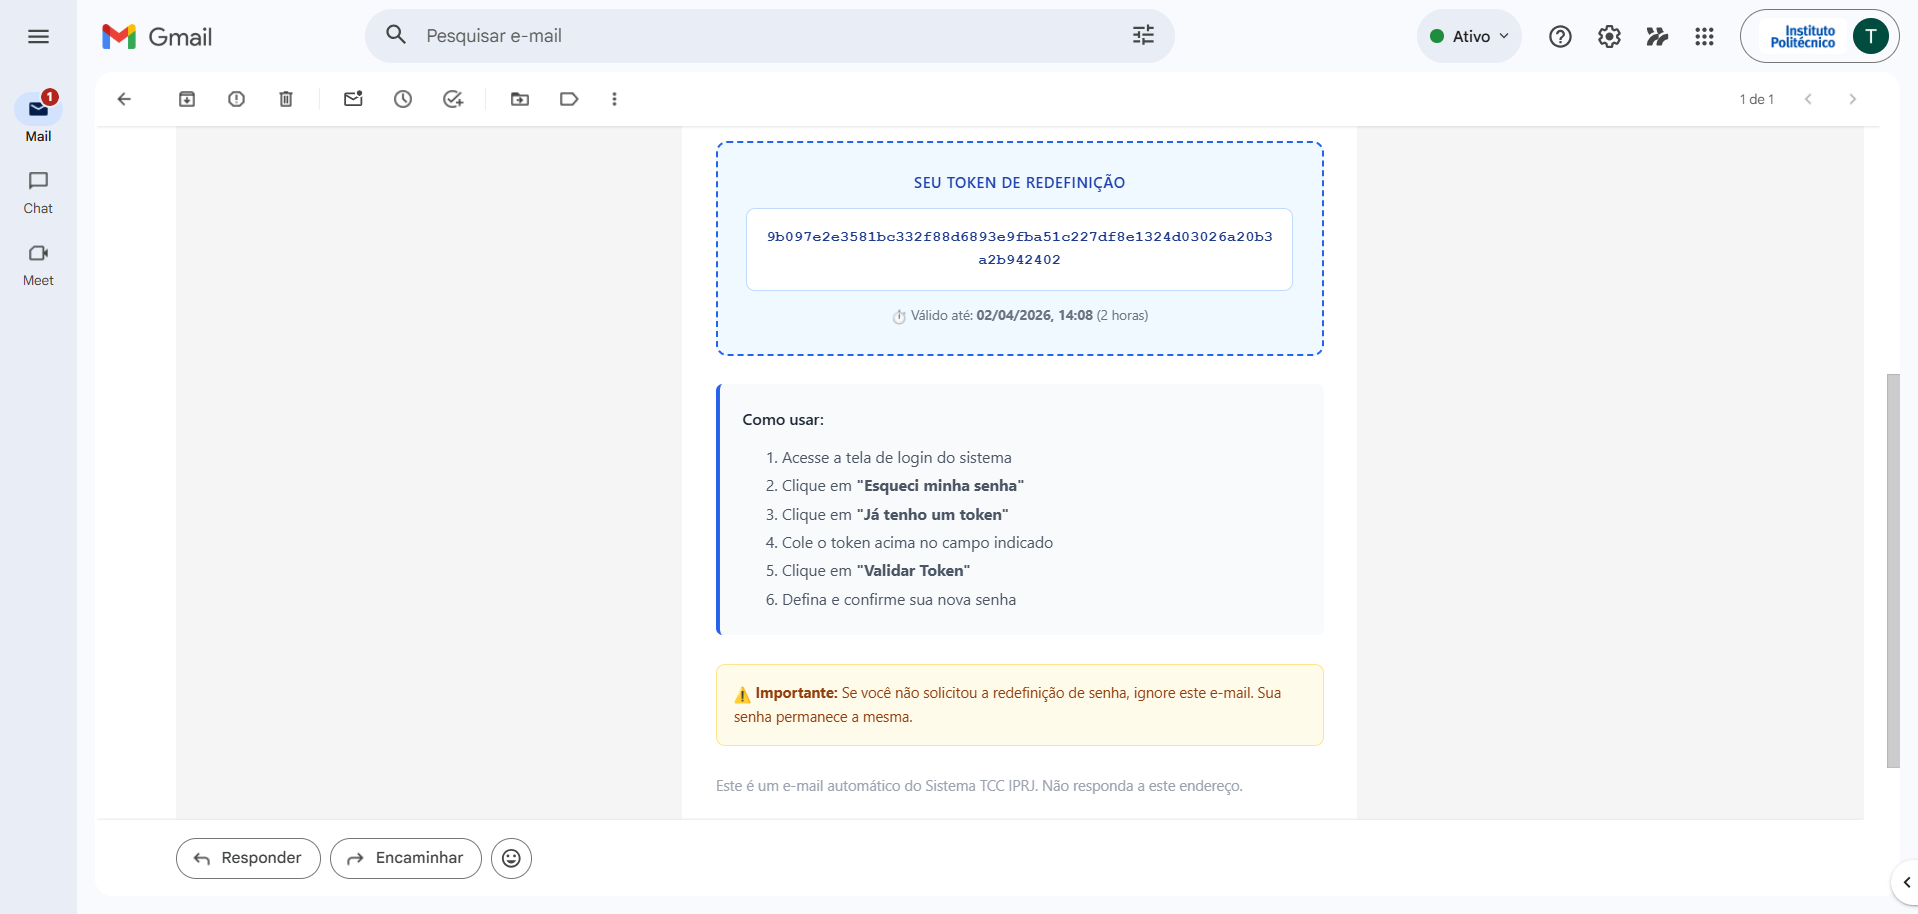
\includegraphics[width=0.75\textwidth]{figures/cap5_reset_email_recebido_pt2.png}
    \caption{Caixa de email com o token de recuperação de senha: token de 64 caracteres e instruções de uso.}
    \label{fig:reset_email_recebido_pt2}
    \fonte{Elaborado pela autora.}
\end{figure}

Com o token em mãos, o administrador acessa a etapa 1, com o formulário de redefinição,
informa o token, conforme ilustra a \autoref{fig:reset_formulario_valida_token}.

\begin{figure}[htbp]
    \centering
    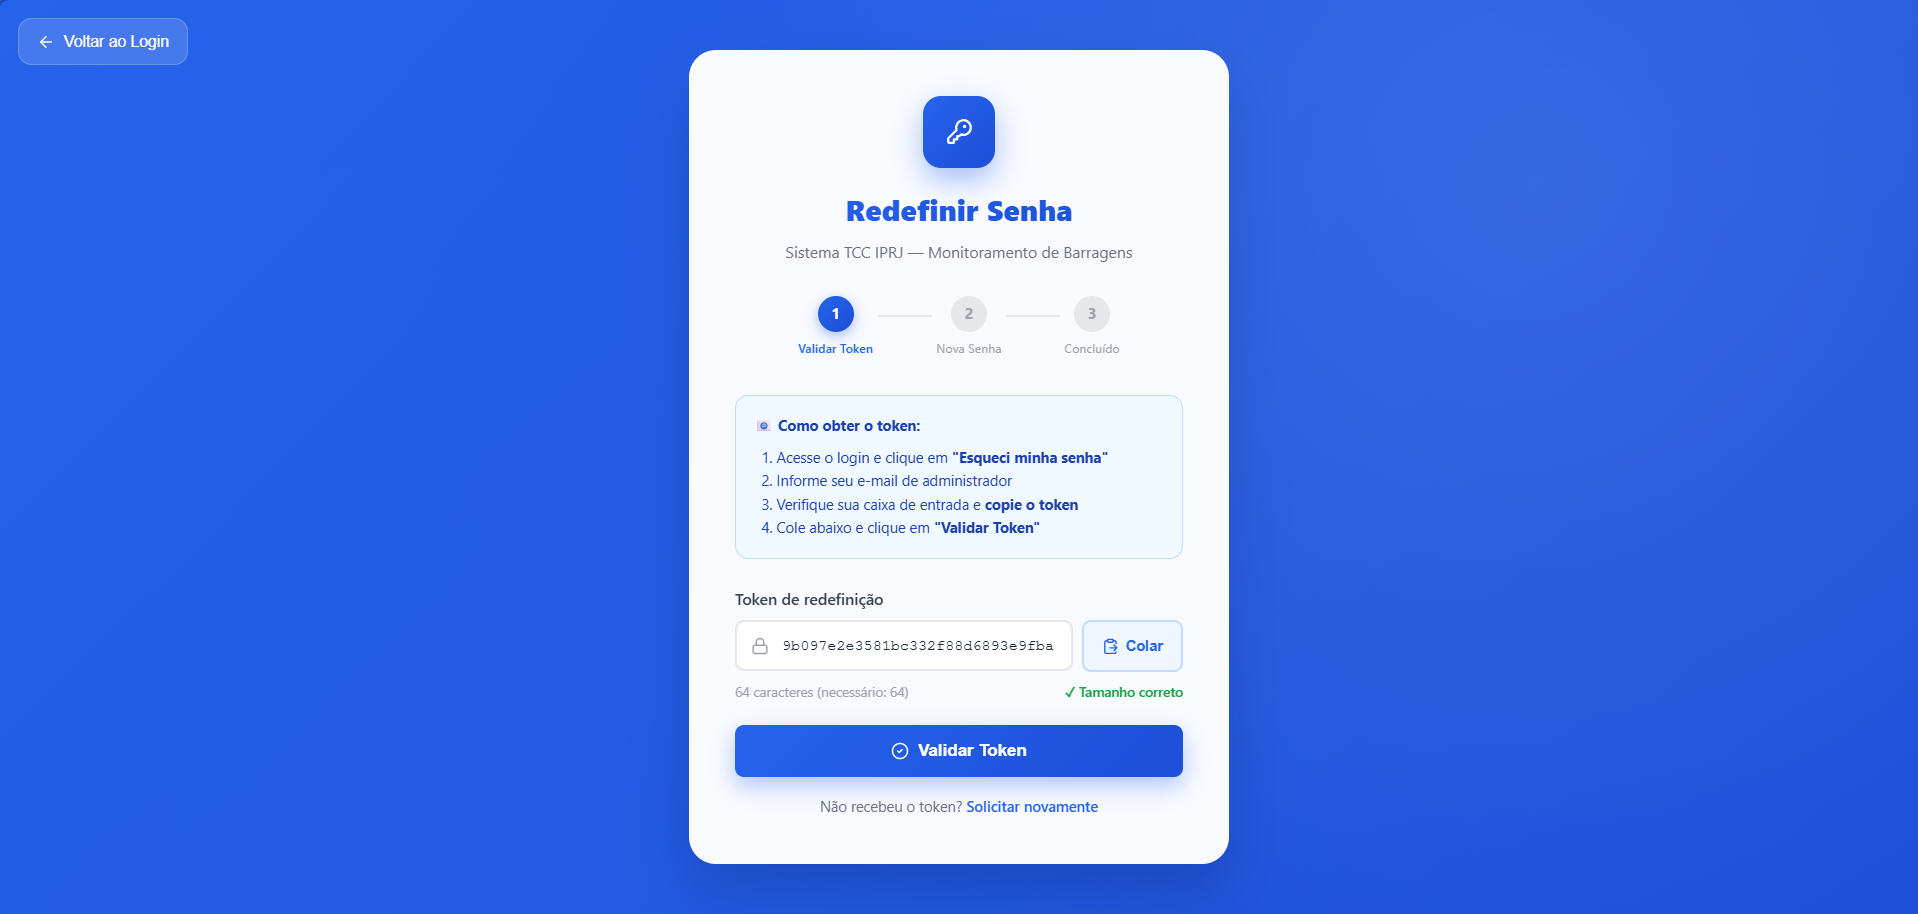
\includegraphics[width=0.75\textwidth]{figures/cap5_reset_formulario_valida_token.png}
    \caption{Etapa 1: Formulário de validação de token}
    \label{fig:reset_formulario_valida_token}
    \fonte{Elaborado pela autora.}
\end{figure}

Ao clicar no botão ``Validar Token'', o sistema exibe a etapa 2, com o formulário para definir a nova senha, com os campos, nova senha e a confirmação, conforme ilustra a \autoref{fig:reset_formulario_nova_senha_pt1}. 
Quando preenche os campos corretamente, conforme ilustra a \autoref{fig:reset_formulario_nova_senha_pt2}, e pressiona o botão ``Redefinir Senha'', a redefinição é bem-sucedida, e o sistema redireciona para a etapa 3, com a mensagem ``Senha redefinida com sucesso!'' e o botão ``Ir para o Login'' para a tela de \textit{login}, conforme mostra a \autoref{fig:reset_formulario_nova_senha_pt3}.

\begin{figure}[htbp]
    \centering
    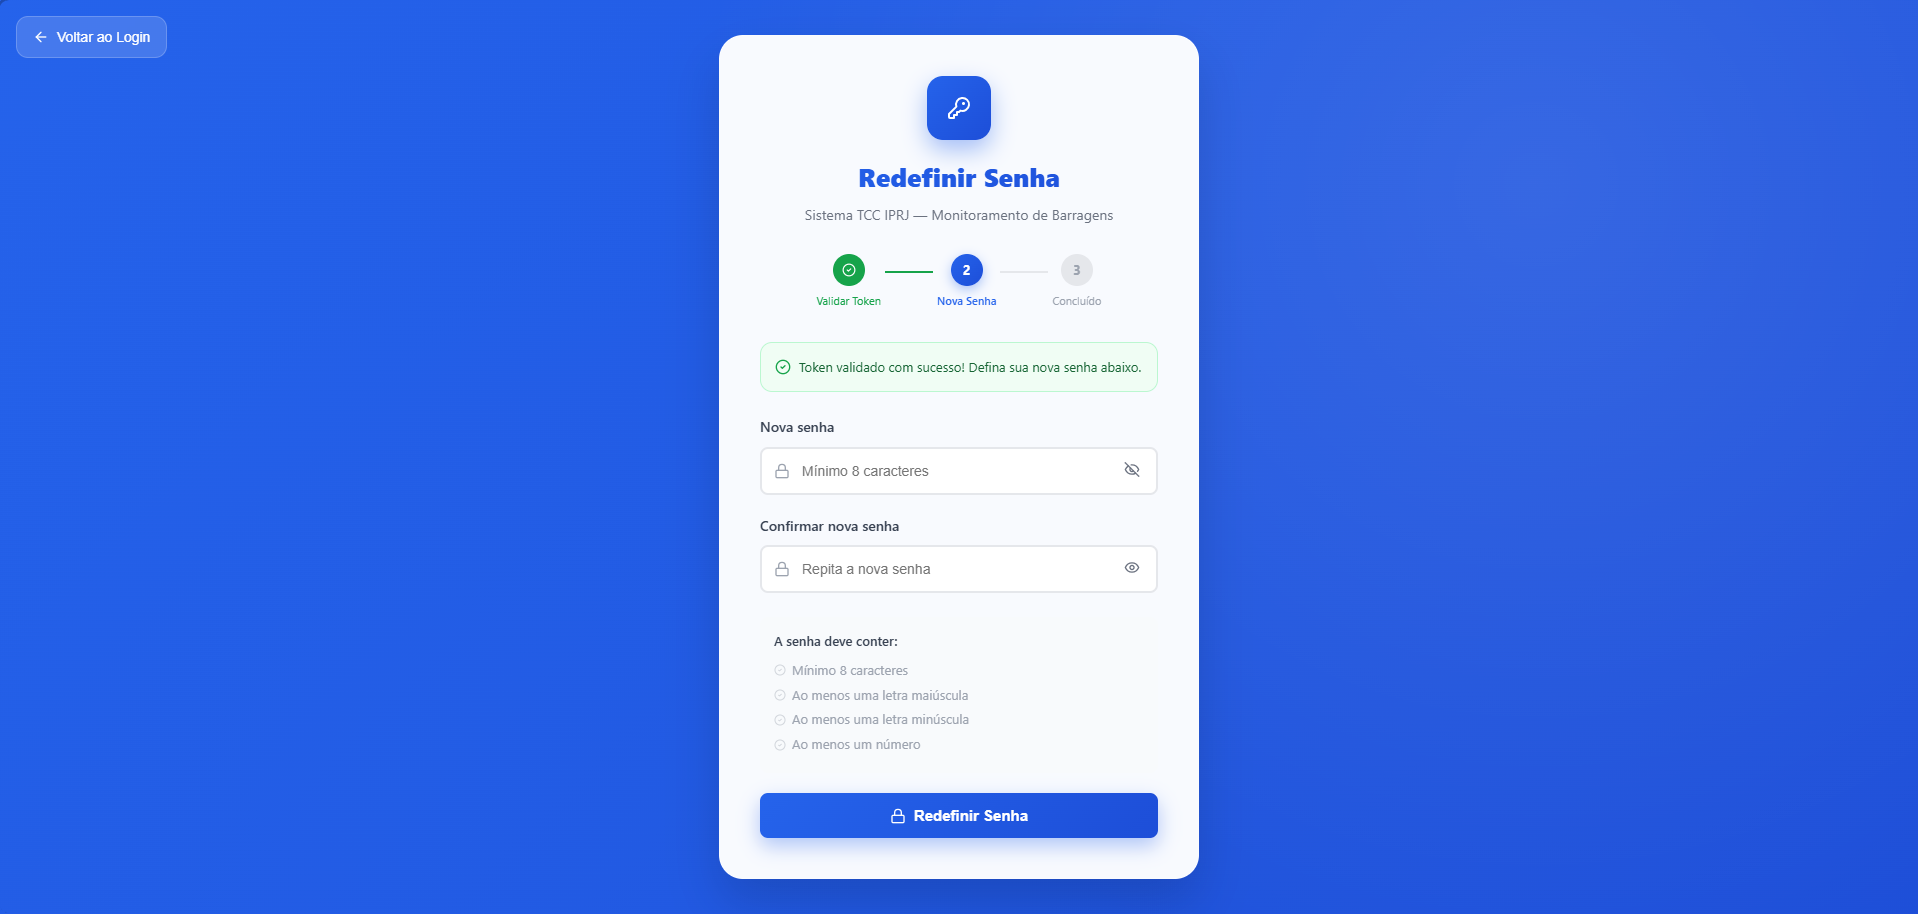
\includegraphics[width=0.75\textwidth]{figures/cap5_reset_formulario_nova_senha_pt1.png}
    \caption{Etapa 2: Formulário de redefinição de senha vazio.}
    \label{fig:reset_formulario_nova_senha_pt1}
    \fonte{Elaborado pela autora.}
\end{figure}

\begin{figure}[htbp]
    \centering
    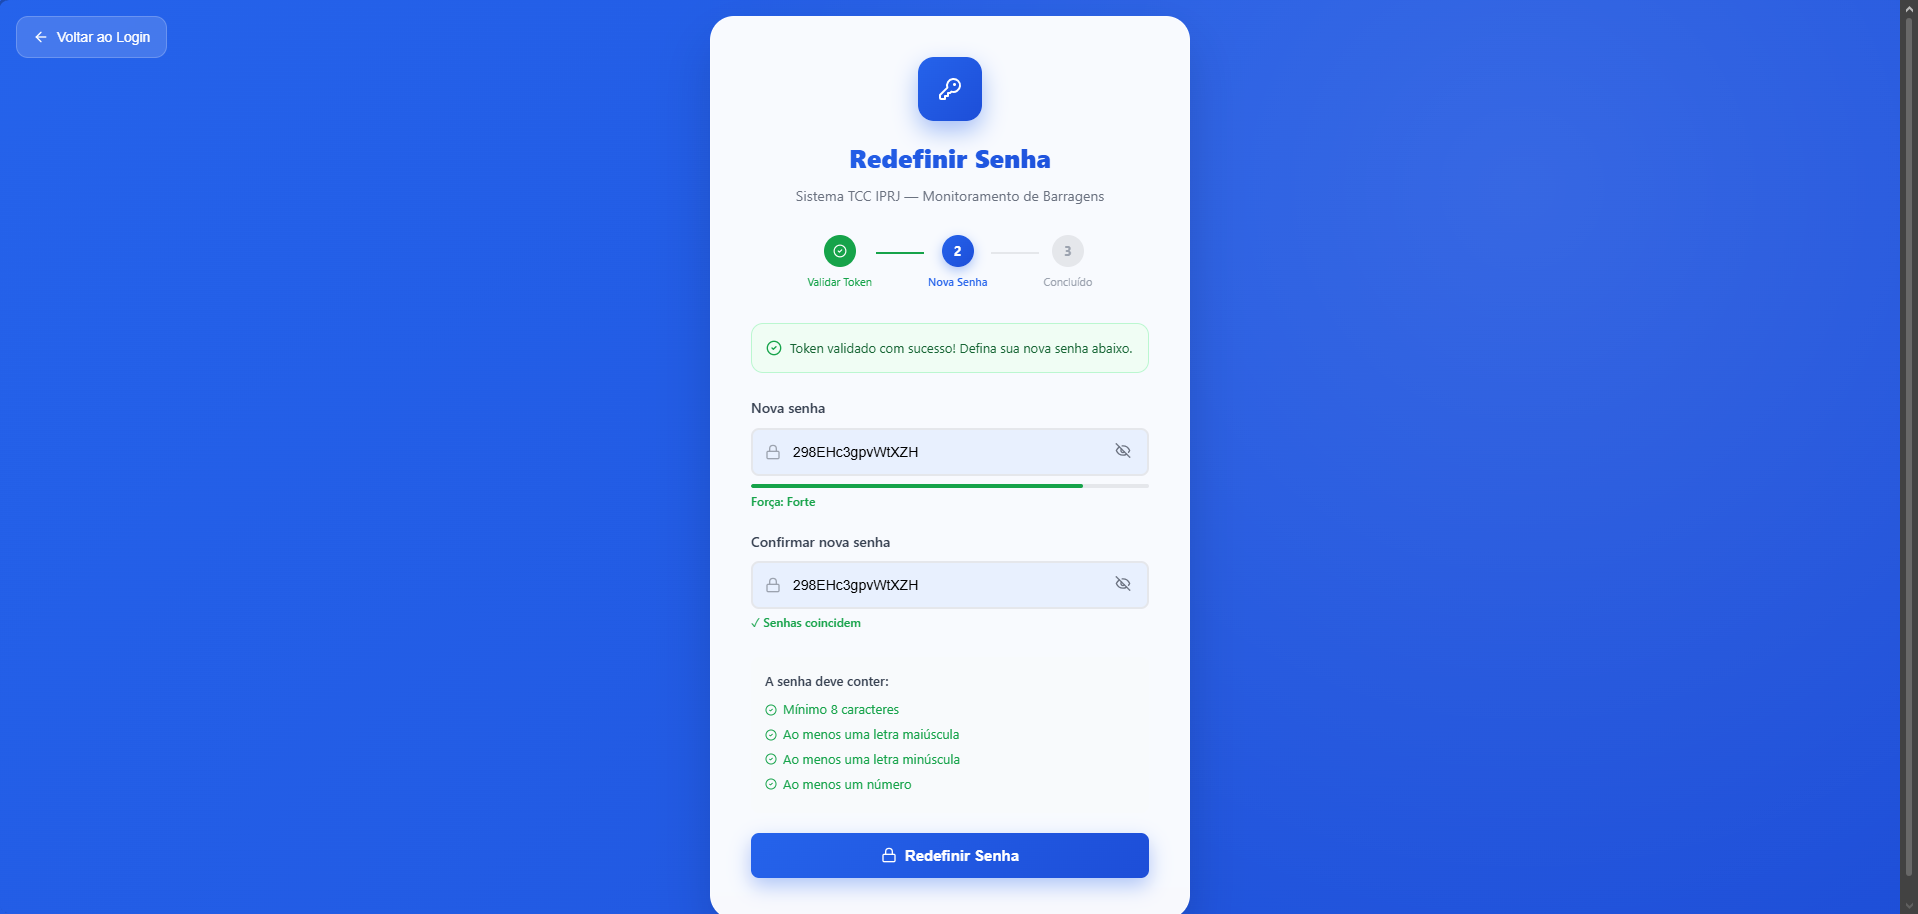
\includegraphics[width=0.75\textwidth]{figures/cap5_reset_formulario_nova_senha_pt2.png}
    \caption{Etapa 2: Formulário de redefinição de senha preenchido - campos de nova senha e confirmação com os critérios de complexidade exibidos preenchidos.}
    \label{fig:reset_formulario_nova_senha_pt2}
    \fonte{Elaborado pela autora.}
\end{figure}

\begin{figure}[htbp]
    \centering
    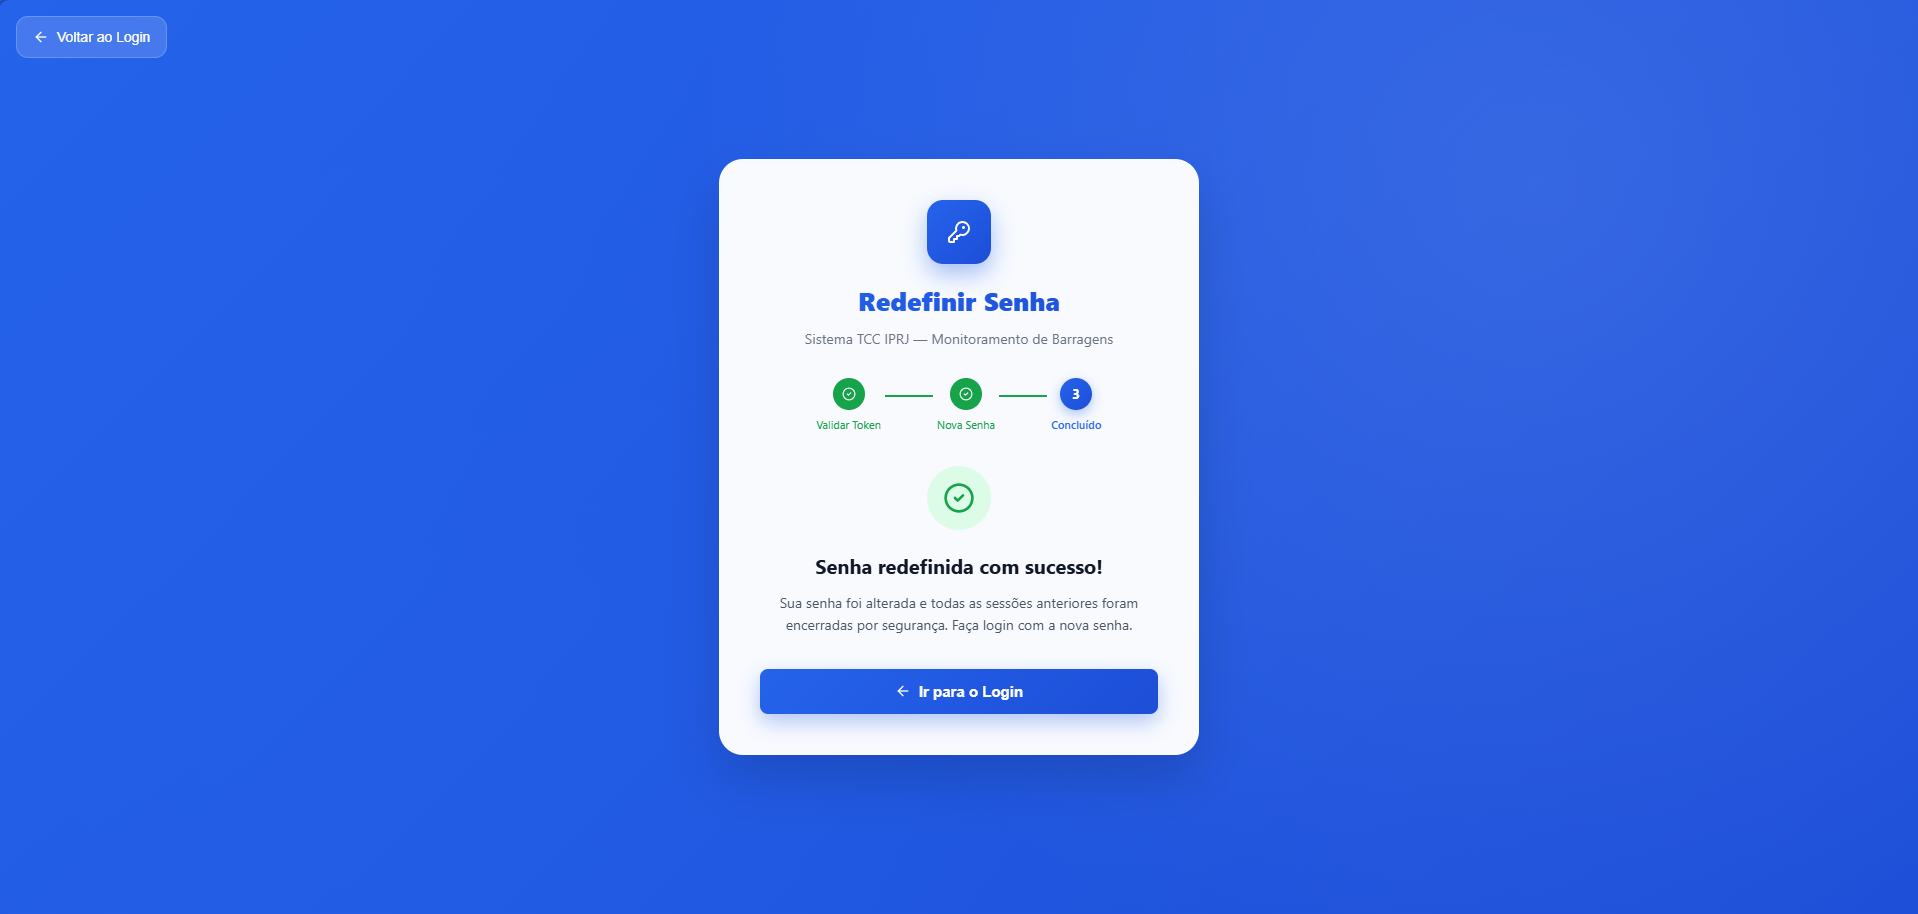
\includegraphics[width=0.75\textwidth]{figures/cap5_reset_formulario_nova_senha_pt3.png}
    \caption{Etapa 3: Modal informativo de senha redefinida com sucesso e botão ``Ir para o Login'' para redirecionamento ao \textit{login} após confirmação.}
    \label{fig:reset_formulario_nova_senha_pt3}
    \fonte{Elaborado pela autora.}
\end{figure}

Se o token for inválido
ou já tiver expirado, o sistema exibe a mensagem ``Token inválido ou
expirado'' e orienta o usuário a solicitar um novo \textit{link}, conforme ilustra a \autoref{fig:reset_token_expirado}.

\begin{figure}[htbp]
    \centering
    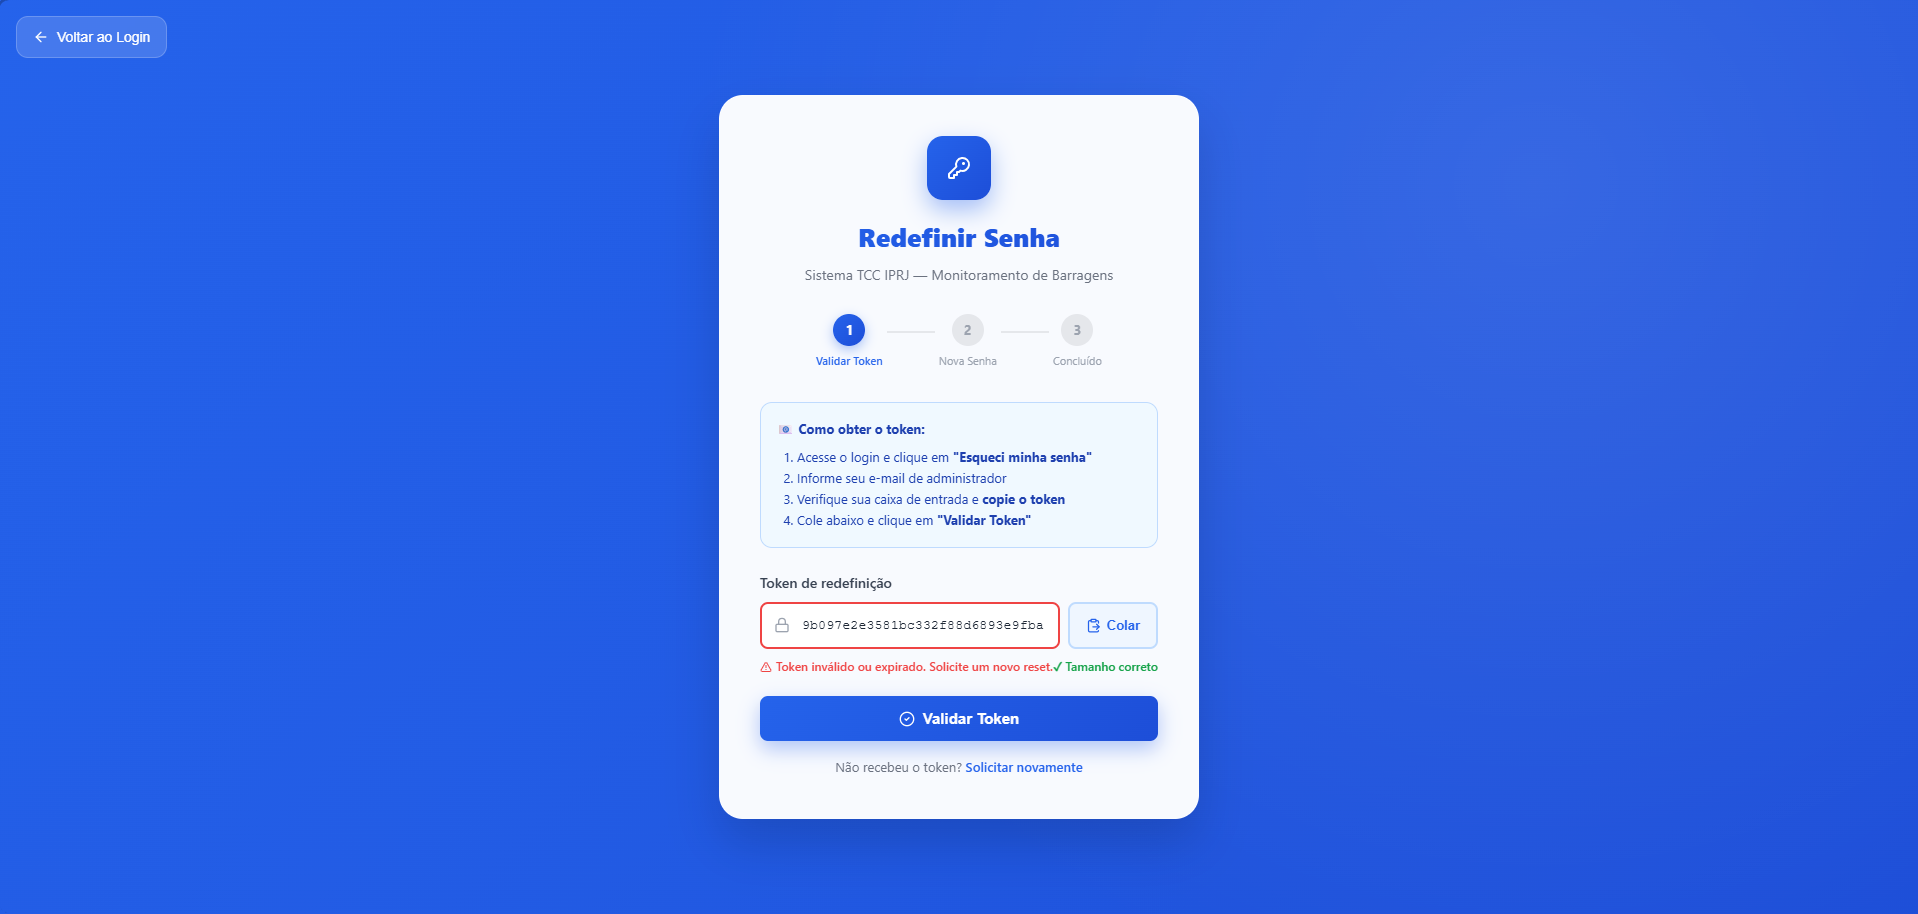
\includegraphics[width=0.75\textwidth]{figures/cap5_reset_token_expirado.png}
    \caption{Tela de redefinição de senha com token inválido ou expirado: mensagem ``Token inválido ou expirado'' e orientação para solicitar novo \textit{link} de recuperação.}
    \label{fig:reset_token_expirado}
    \fonte{Elaborado pela autora.}
\end{figure}

Senhas
que não atendam ao critério mínimo --- ao menos 6 caracteres, com
letras maiúsculas, minúsculas e um número --- são recusadas com mensagem
de erro inline antes mesmo do envio ao servidor, conforme ilustra a \autoref{fig:reset_senha_padrao_invalido}.

\begin{figure}[htbp]
    \centering
    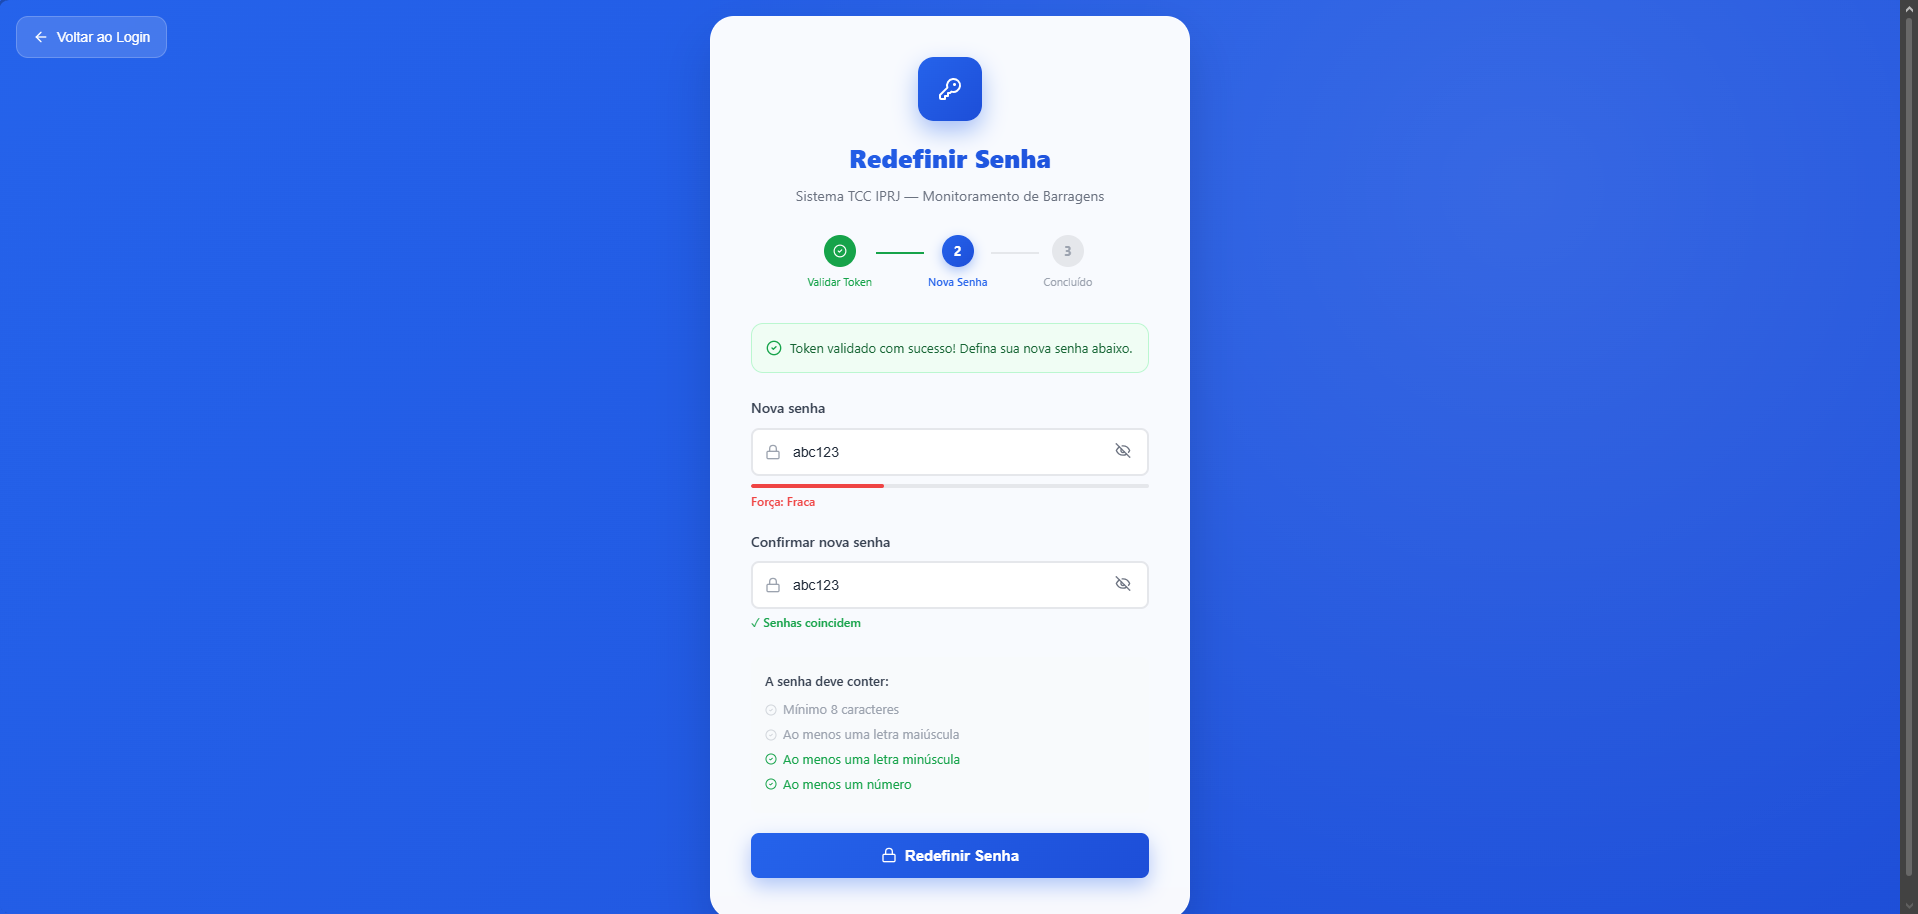
\includegraphics[width=0.75\textwidth]{figures/cap5_reset_senha_padrao_invalido.png}
    \caption{Formulário de redefinição com mensagem de erro inline: nova senha não atende aos critérios mínimos de complexidade; formulário retorna para correção sem enviar ao \textit{backend}.}
    \label{fig:reset_senha_padrao_invalido}
    \fonte{Elaborado pela autora.}
\end{figure}

% =============================================================
\section{\textit{Dashboard} --- Monitoramento em Tempo Real}
\label{sec:dashboard}
% =============================================================

O \textit{dashboard} é a primeira tela exibida após o \textit{login} e
a central de monitoramento do sistema. Ao carregá-lo, o administrador
visualiza de imediato o estado atual da barragem, os principais
indicadores das últimas 24 horas e a situação das integrações externas.

% -------------------------------------------------------------
\subsection{Sistema em Nível VERDE}
\label{subsec:dashboard-verde}
% -------------------------------------------------------------

Quando o índice de risco integrado não supera 45\%, o \textit{dashboard}
apresenta borda verde ao redor do card de situação atual, identificando
a condição como segura. A \autoref{fig:dashboard_verde} ilustra essa
configuração: o fator de risco exibido em porcentagem, os cinco KPIs
resumindo as últimas 24 horas --- total de leituras, umidade média, risco
médio, precipitação média e alertas críticos --- o gráfico histórico com
as séries de umidade, precipitação e risco, e o painel lateral com o
status das APIs BNDMET e OWM, o estado do sensor e a recomendação
operacional gerada pelo dispositivo.

\begin{figure}[htbp]
    \centering
    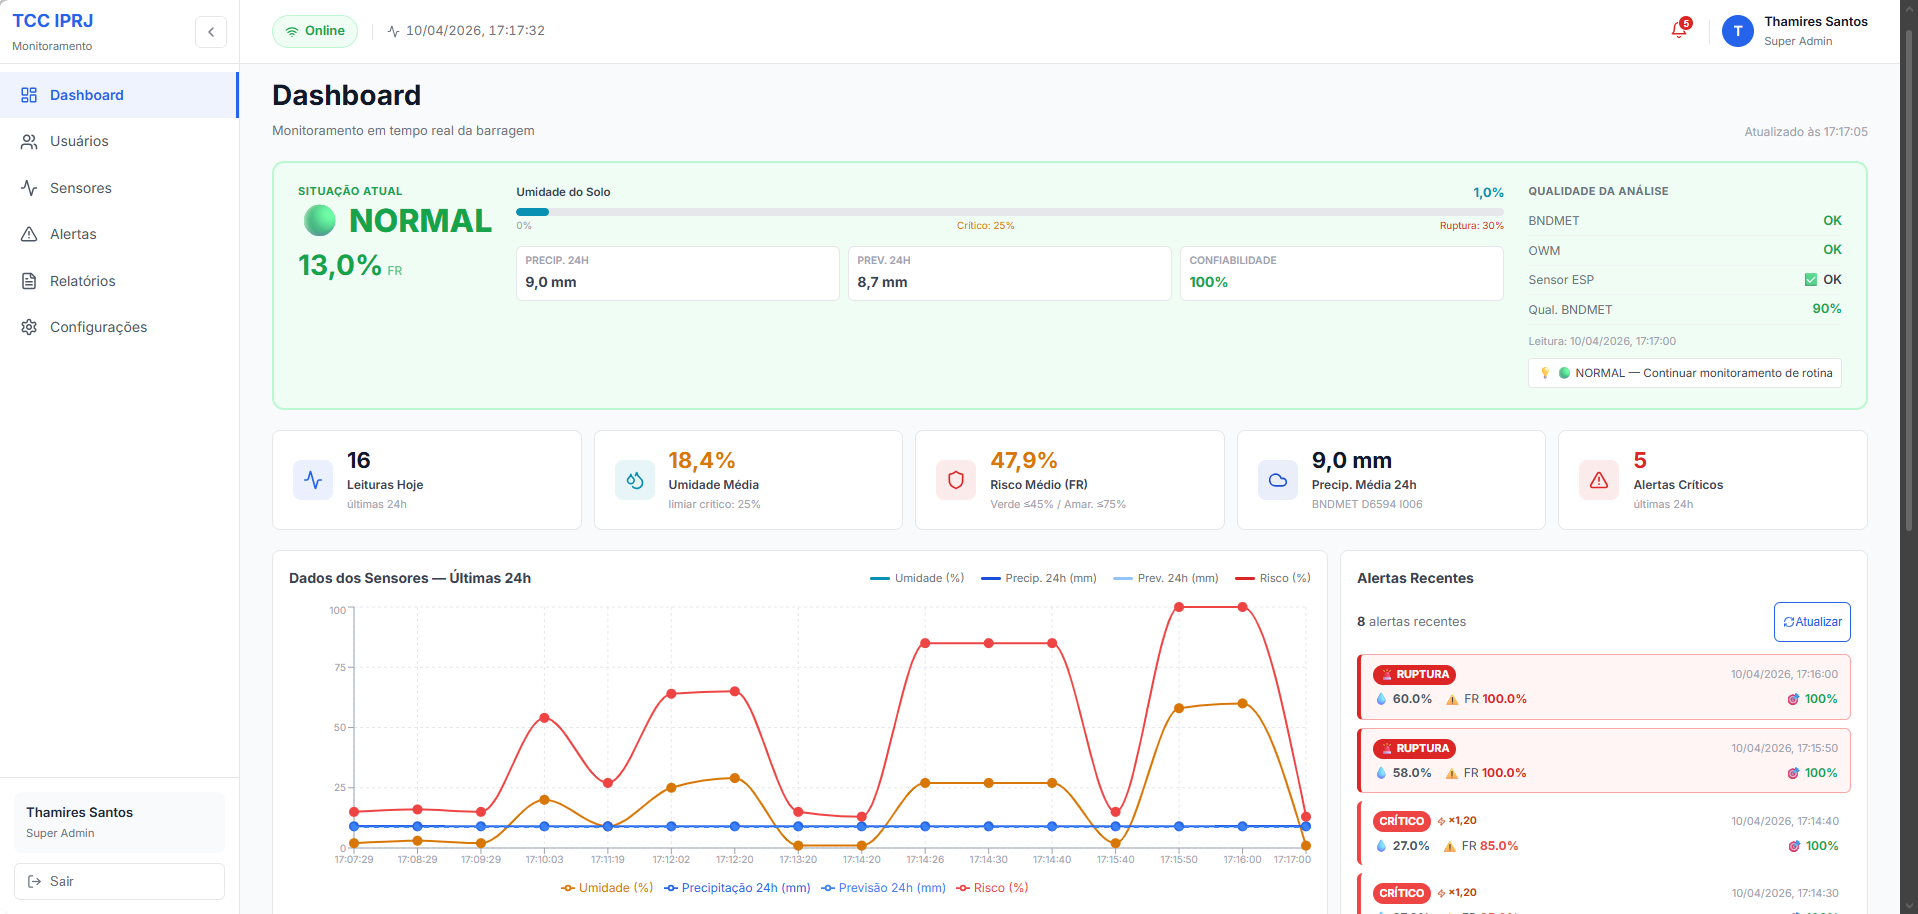
\includegraphics[width=0.95\textwidth]{figures/cap5_dashboard_verde.png}
    \caption{\textit{Dashboard} com sistema em nível VERDE: borda verde
    no card de situação, KPIs das últimas 24 horas, gráfico histórico e
    painel de status das APIs e do sensor.}
    \label{fig:dashboard_verde}
    \fonte{Elaborado pela autora.}
\end{figure}

% -------------------------------------------------------------
\subsection{Sistema em Nível AMARELO}
\label{subsec:dashboard-amarelo}
% -------------------------------------------------------------

Com o índice de risco entre 46\% e 75\%, o card de situação atual
assume borda amarela e o rótulo muda para ``ATENÇÃO''. A
\autoref{fig:dashboard_amarelo} mostra essa configuração, com o KPI
de alertas críticos incrementado em relação ao estado anterior.

\begin{figure}[htbp]
    \centering
    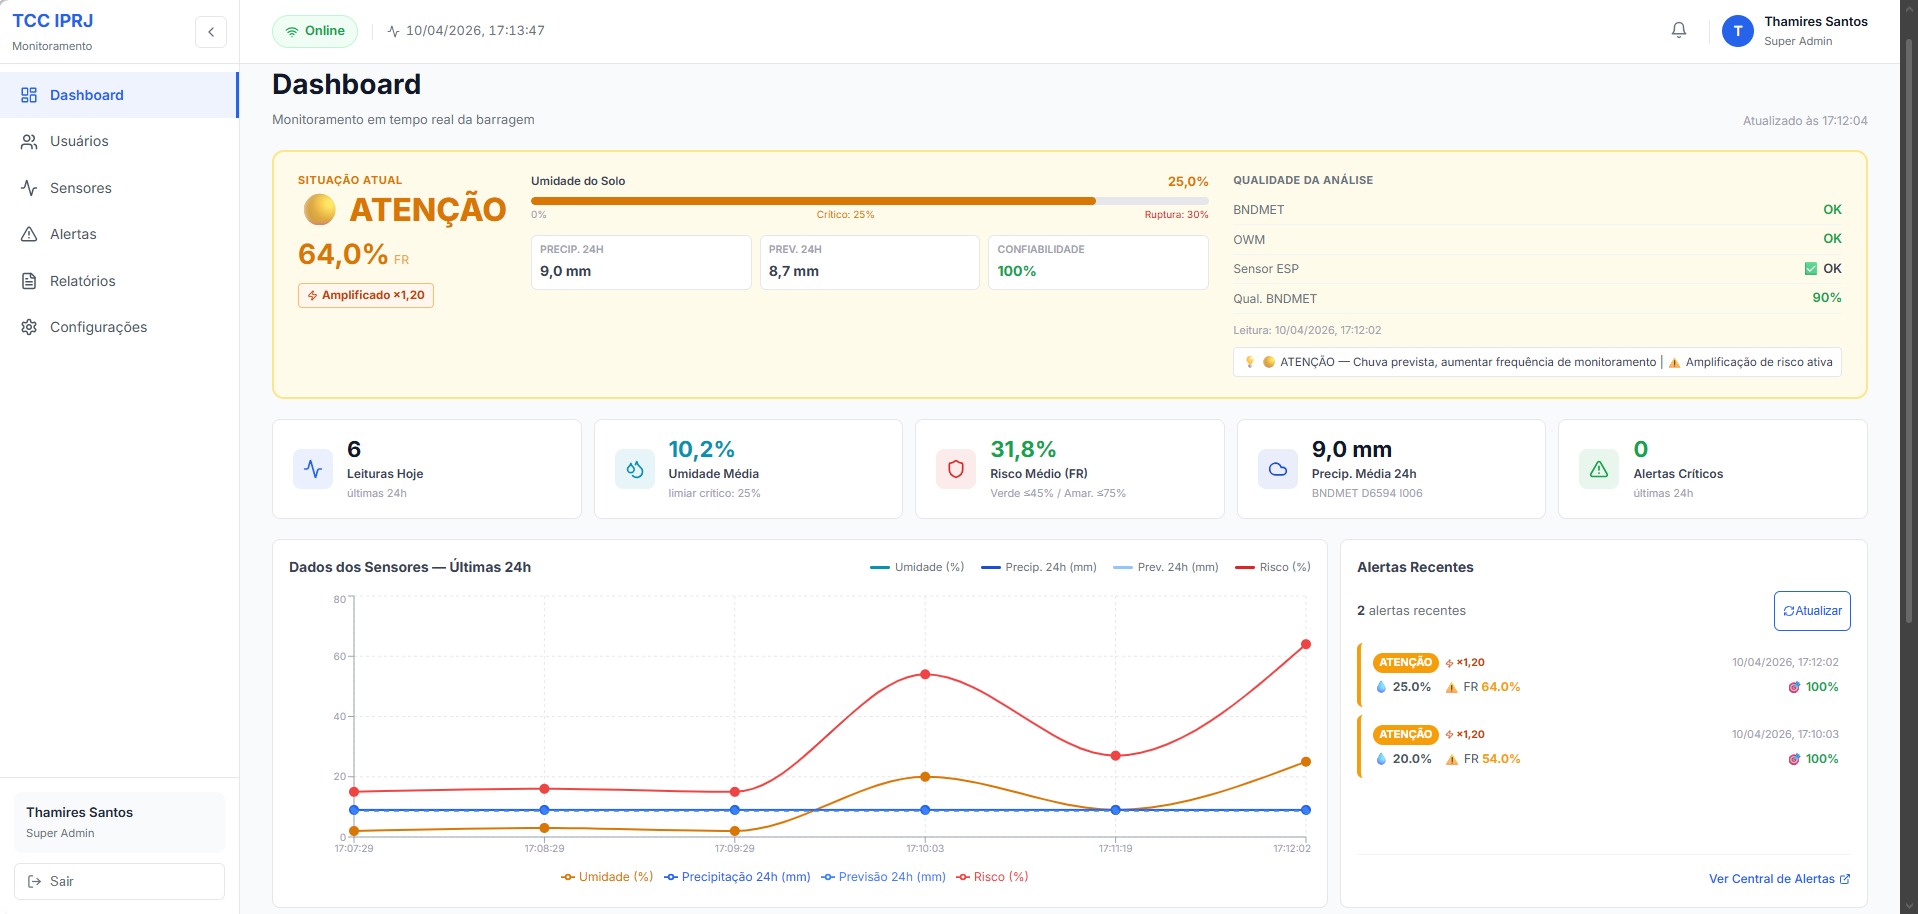
\includegraphics[width=0.95\textwidth]{figures/cap5_dashboard_amarelo.png}
    \caption{\textit{Dashboard} com sistema em nível AMARELO: borda
    amarela no card de situação, índice de risco entre 46 e 75\% e KPI
    de alertas críticos atualizado.}
    \label{fig:dashboard_amarelo}
    \fonte{Elaborado pela autora.}
\end{figure}

% -------------------------------------------------------------
\subsection{Sistema em Nível VERMELHO}
\label{subsec:dashboard-vermelho}
% -------------------------------------------------------------

Acima de 75\% no índice de risco, o card assume borda vermelha e o
rótulo ``CRÍTICO''. Quando o mecanismo de amplificação está ativo, o
\textit{badge} ``Amplificado $\times 1{,}20$'' aparece em laranja
imediatamente abaixo do índice, como demonstra a
\autoref{fig:dashboard_vermelho}. O sino de notificações no
\textit{header} exibe um indicador de alerta crítico pendente.

\begin{figure}[htbp]
    \centering
    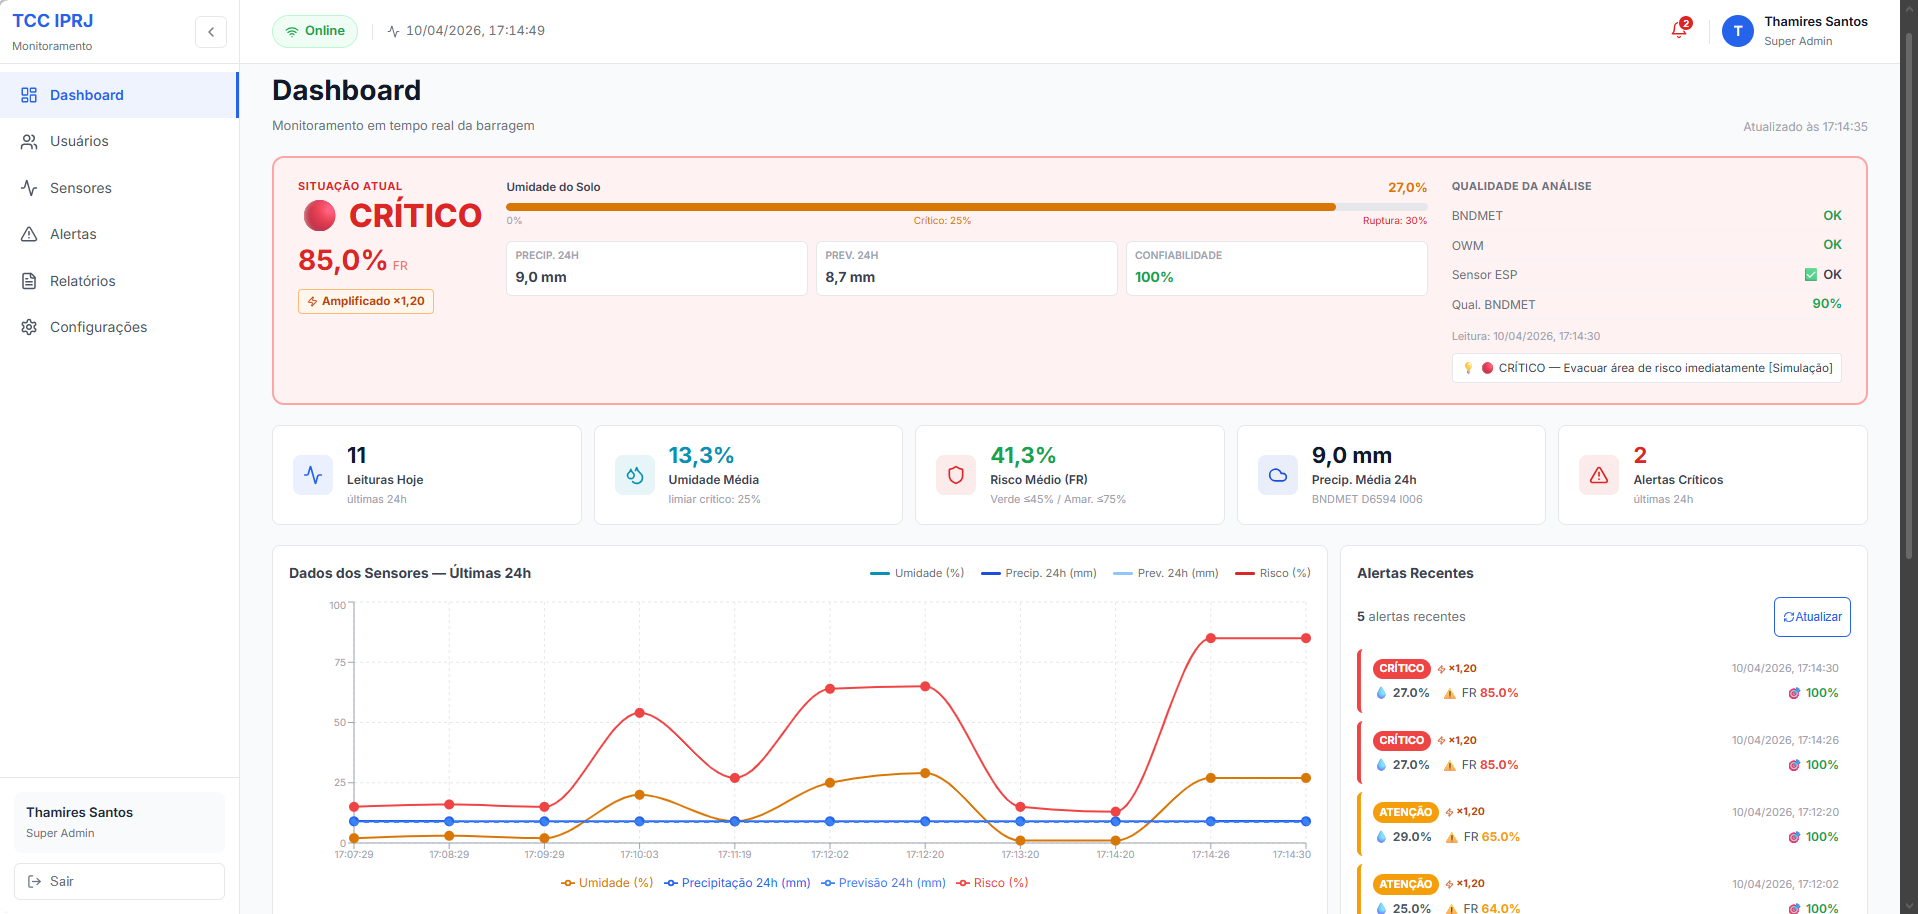
\includegraphics[width=0.95\textwidth]{figures/cap5_dashboard_vermelho.png}
    \caption{\textit{Dashboard} com sistema em nível VERMELHO: borda
    vermelha, índice acima de 75\% e, quando aplicável, \textit{badge}
    ``Amplificado $\times 1{,}20$'' em laranja.}
    \label{fig:dashboard_vermelho}
    \fonte{Elaborado pela autora.}
\end{figure}

% -------------------------------------------------------------
\subsection{Sistema em Nível RUPTURA}
\label{subsec:dashboard-ruptura}
% -------------------------------------------------------------

Quando a umidade do solo atinge ou supera 30\%, o protocolo de ruptura
é acionado de forma imediata e o \textit{dashboard} assume sua
representação visual mais crítica: borda roxa ao redor do card de
situação atual e rótulo ``RUPTURA'' em destaque. Esse estado independe
do índice calculado pelos sete componentes do modelo --- a leitura
direta do sensor é suficiente para acionar o protocolo, conforme
demonstra a \autoref{fig:dashboard_ruptura}. O sino de notificações
no \textit{header} exibe um indicador de alerta crítico pendente,
e o intervalo de transmissão do dispositivo é reduzido para 5 segundos.

\begin{figure}[htbp]
    \centering
    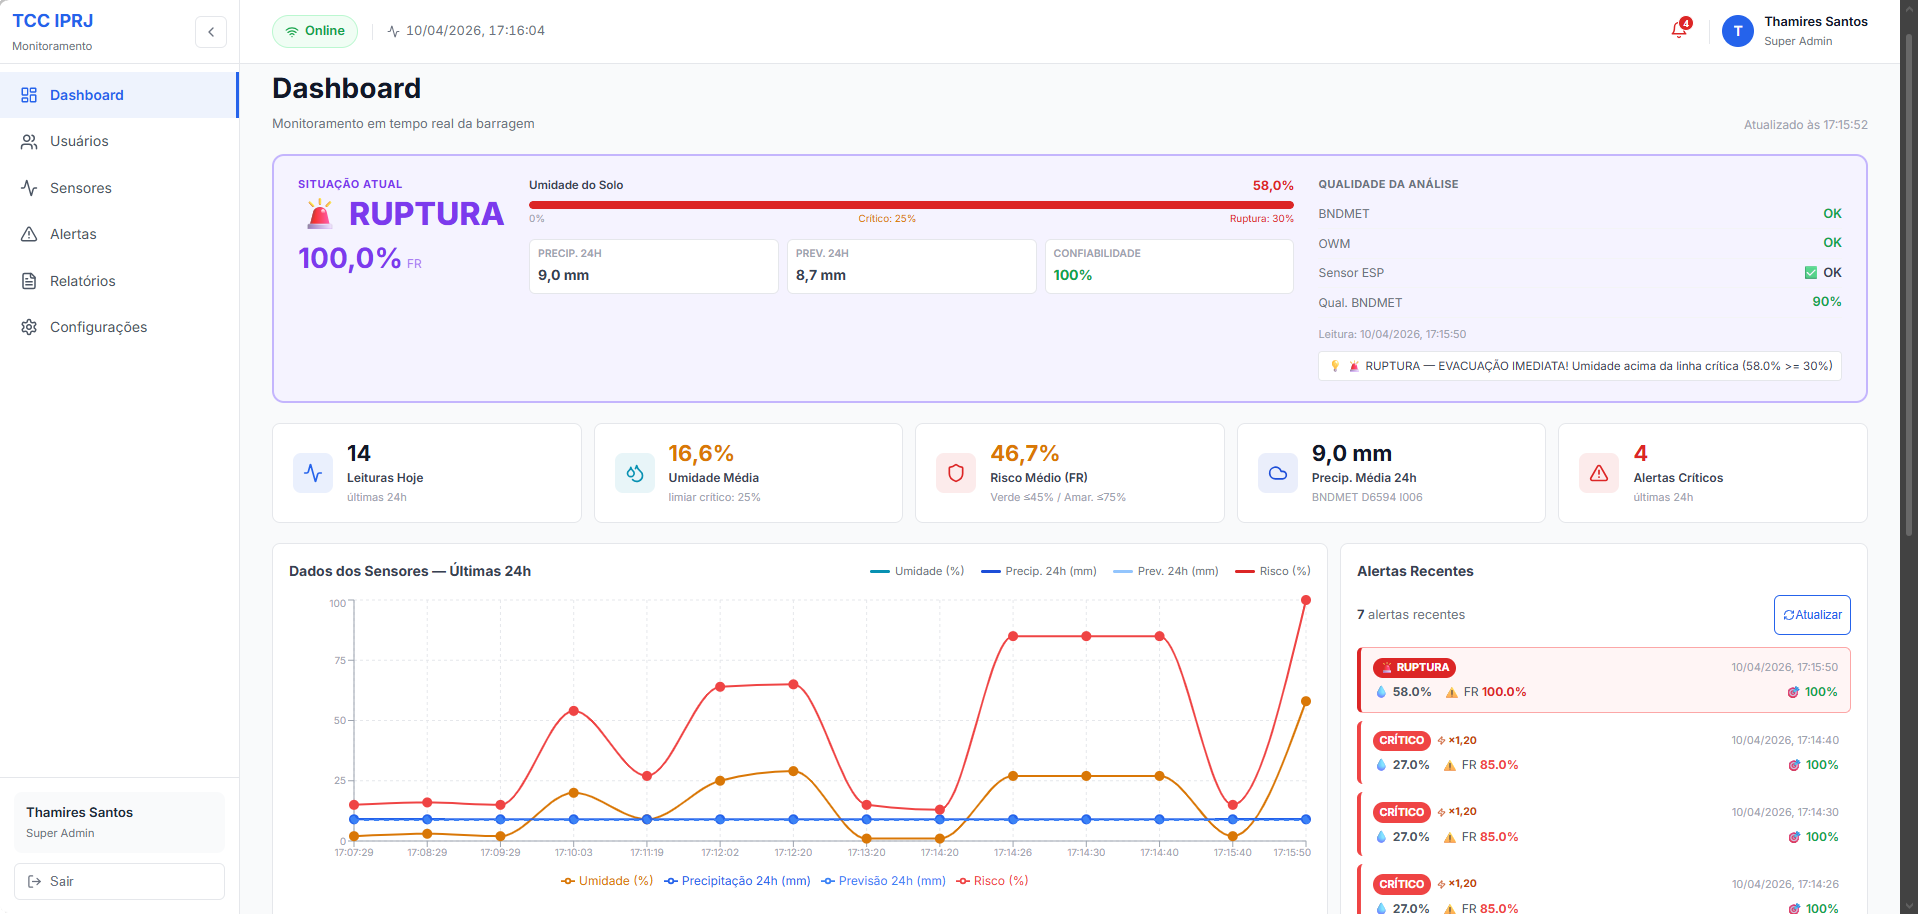
\includegraphics[width=0.95\textwidth]{figures/cap5_dashboard_ruptura.png}
    \caption{\textit{Dashboard} com sistema em estado de RUPTURA: borda
    roxa no card de situação, rótulo ``RUPTURA'' e indicador de alerta
    crítico no \textit{header}; protocolo acionado quando a umidade
    do solo atinge ou supera 30\%.}
    \label{fig:dashboard_ruptura}
    \fonte{Elaborado pela autora.}
\end{figure}

% -------------------------------------------------------------
\subsection{Atividade Recente, Gráfico Histórico e Status do Sistema}
\label{subsec:dashboard-atividade}
% -------------------------------------------------------------

O gráfico histórico (\autoref{fig:dashboard_grafico}) sobrepõe quatro
séries temporais referentes às últimas 24 horas: umidade do solo,
precipitação acumulada de 24 horas, previsão de precipitação e índice
de risco. Ao posicionar o cursor sobre qualquer ponto do gráfico, um
\textit{tooltip} exibe os valores exatos das quatro séries naquele
instante.

A parte inferior do \textit{dashboard} apresenta dois painéis
complementares (\autoref{fig:dashboard_grafico_inferior}). O painel de atividade recente lista as últimas
interações do sistema --- leituras recebidas, alertas registrados e
eventos de conectividade --- com rótulos de tempo relativo. O painel
meteorológico exibe temperatura, umidade relativa do ar, pressão
atmosférica e velocidade do vento da última leitura disponível.

\begin{figure}[htbp]
    \centering
    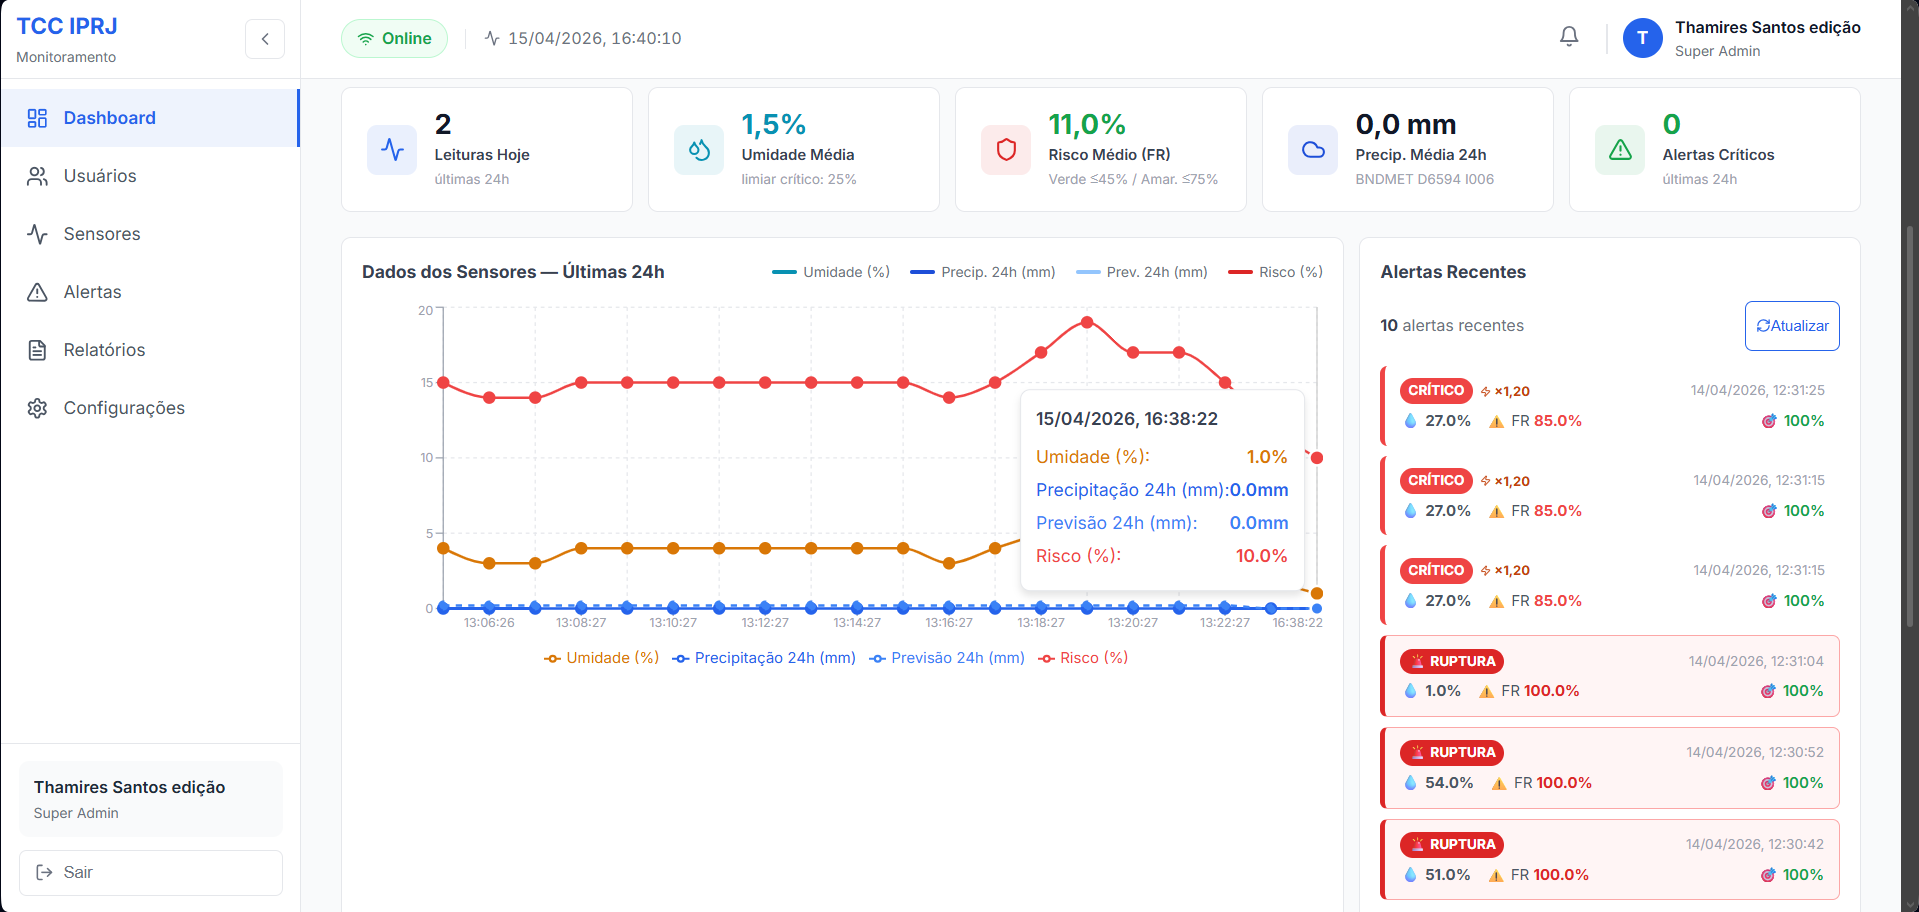
\includegraphics[width=0.95\textwidth]{figures/cap5_dashboard_grafico.png}
    \caption{Gráfico histórico com quatro séries temporais das últimas
    24 horas: umidade do solo, precipitação acumulada, previsão de
    chuva e índice de risco integrado.}
    \label{fig:dashboard_grafico}
    \fonte{Elaborado pela autora.}
\end{figure}

\begin{figure}[htbp]
    \centering
    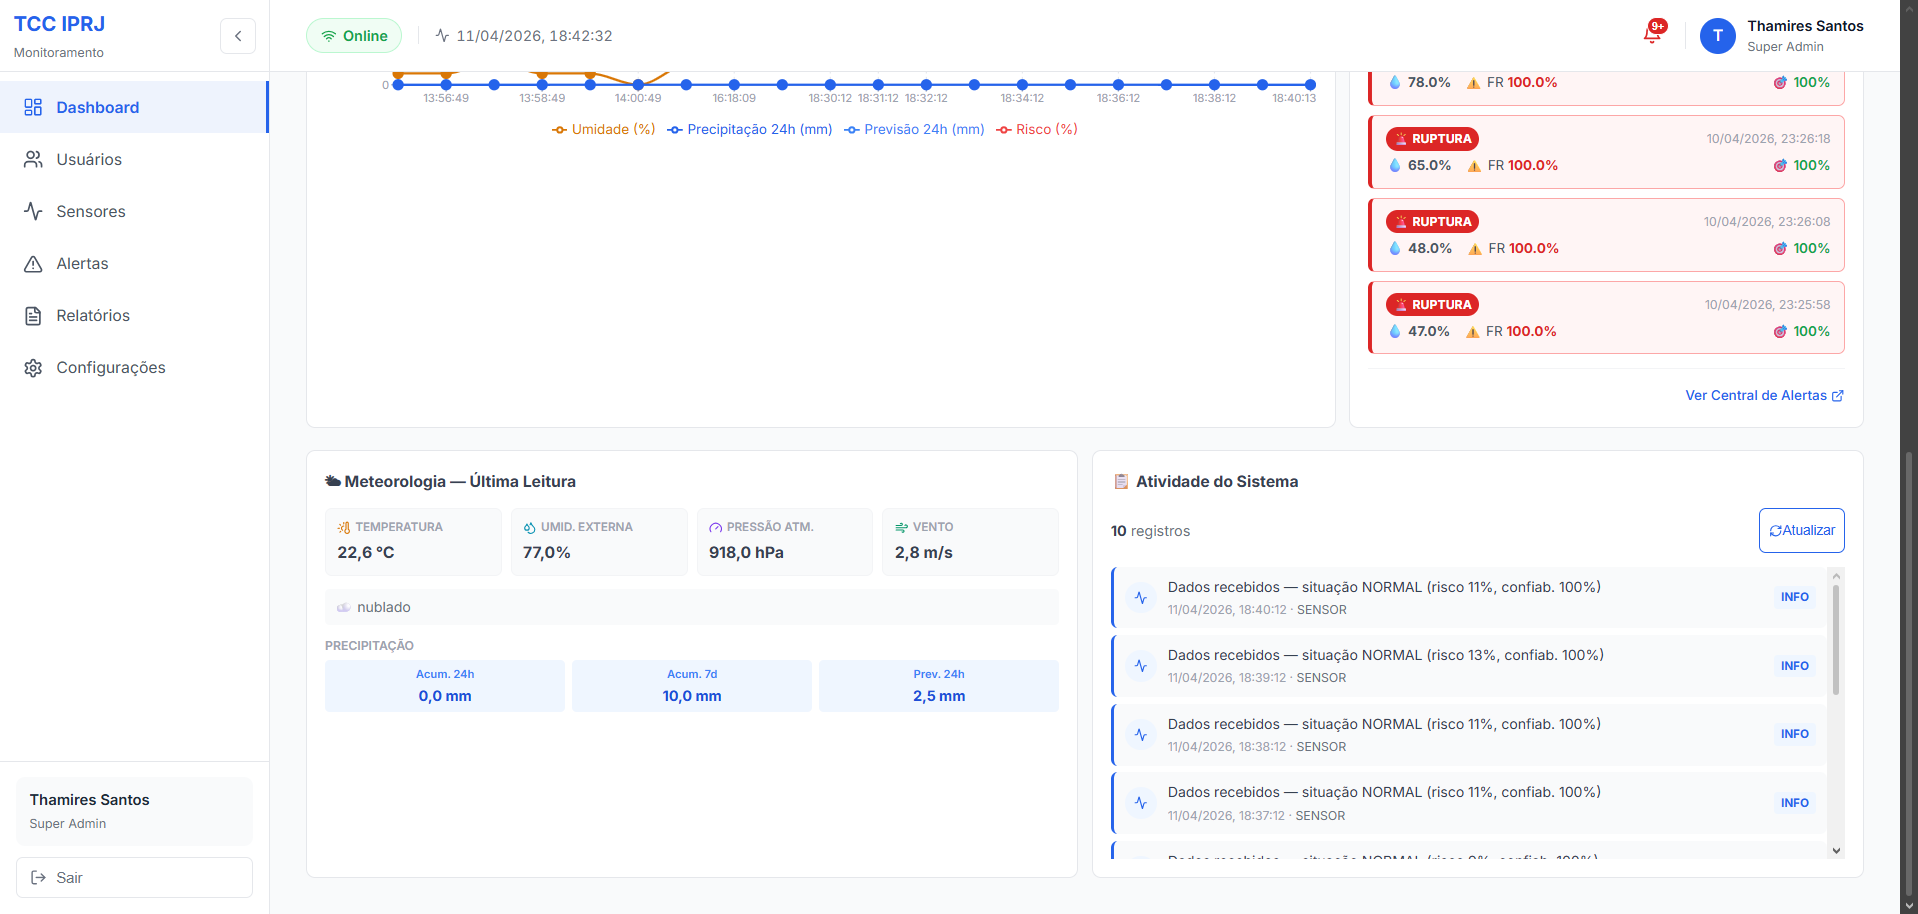
\includegraphics[width=0.95\textwidth]{figures/cap5_dashboard_grafico_inferior.png}
    \caption{Parte inferior do \textit{dashboard}: painel de atividade recente e painel meteorológico.}
    \label{fig:dashboard_grafico_inferior}
    \fonte{Elaborado pela autora.}
\end{figure}

Em condições normais de operação, o \textit{header} exibe o status "Online" em verde, 
confirmando que o dispositivo embarcado está enviando leituras dentro do intervalo 
esperado, conforme ilustra a \autoref{fig:dashboard_verde}. Esse indicador
é atualizado a cada 30 segundos pela consulta de saúde do \textit{backend},
e as notificações de novos alertas são verificadas a cada 60 segundos.

Quando o sensor para de enviar dados por mais de 3 minutos, o indicador
no \textit{header} passa a exibir ``Degradado'' em laranja, conforme
ilustra a \autoref{fig:dashboard_degradado}. Esse estado reflete um
atraso nas leituras do dispositivo embarcado, mas o sistema continua
operacional: o \textit{backend} e o banco de dados permanecem acessíveis
e os KPIs exibem os valores da última leitura disponível.

\begin{figure}[htbp]
    \centering
    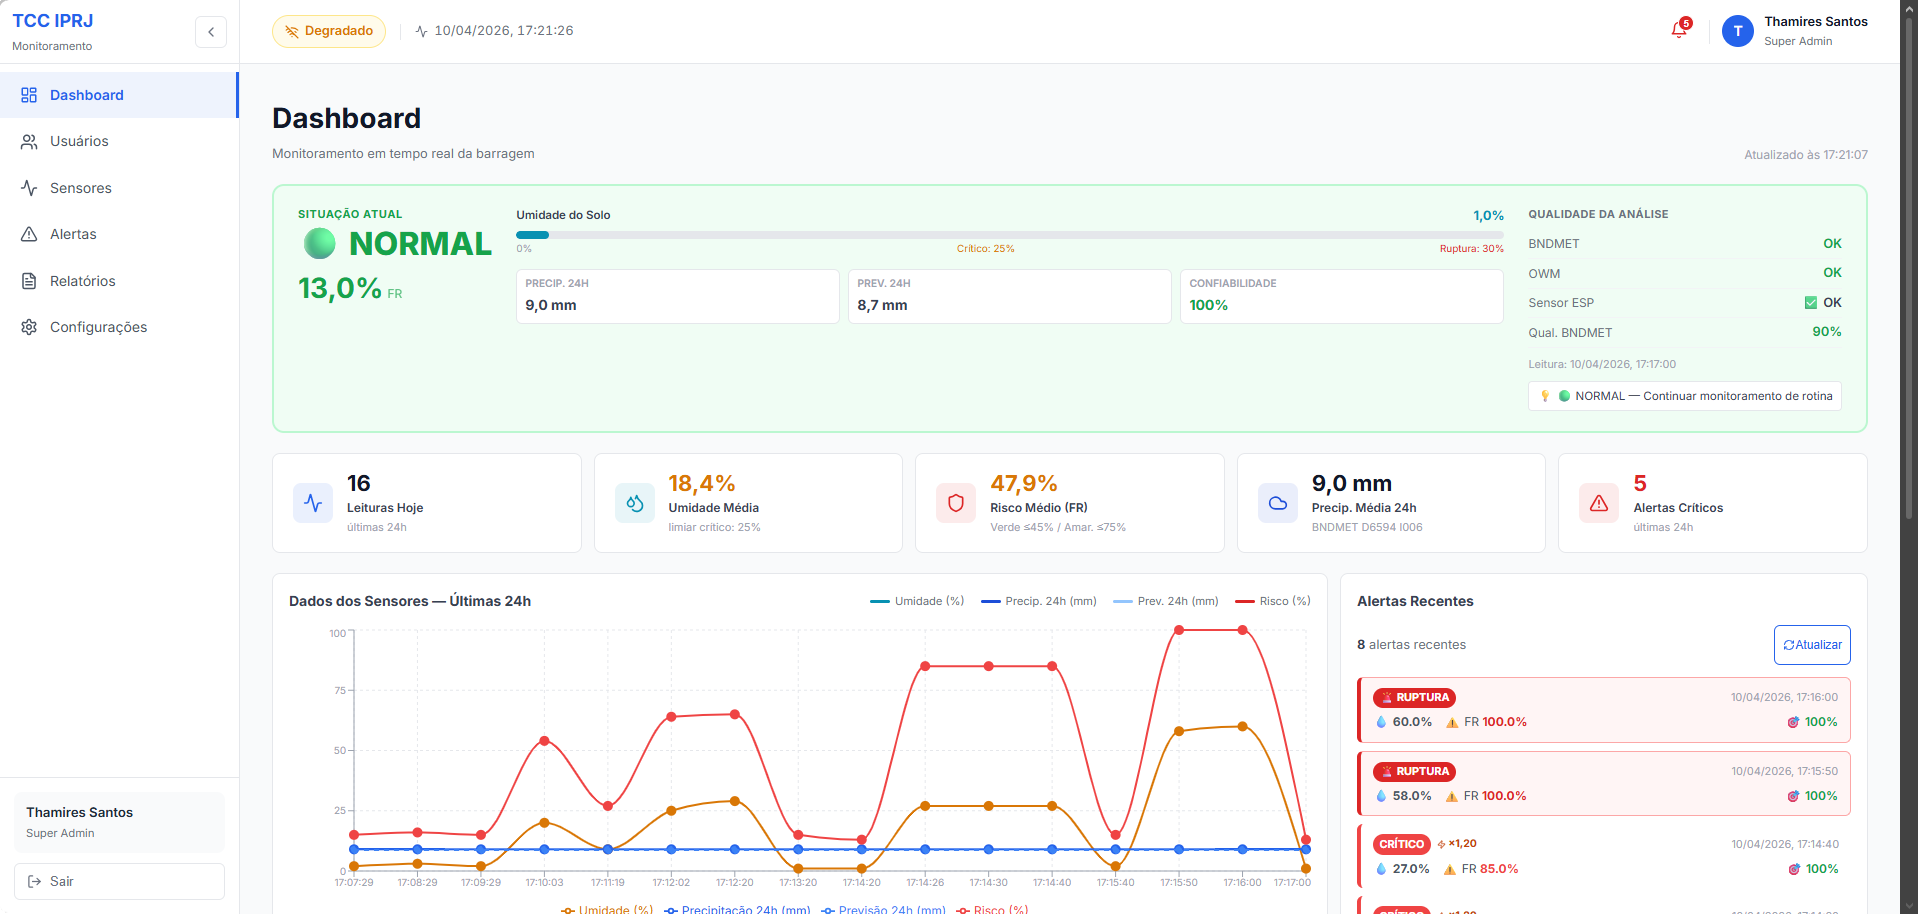
\includegraphics[width=0.95\textwidth]{figures/cap5_dashboard_degradado.png}
    \caption{\textit{Header} do \textit{dashboard} com status ``Degradado''
    em laranja: sensor sem envio de dados há mais de 3 minutos; demais
    KPIs exibidos com os valores da última leitura disponível.}
    \label{fig:dashboard_degradado}
    \fonte{Elaborado pela autora.}
\end{figure}

Quando o próprio \textit{backend} fica inacessível --- por desligamento
do servidor ou falha de rede local ---, o \textit{frontend} não consegue
completar a verificação de saúde e força o estado mais grave: o indicador
muda para ``Offline'' em vermelho, conforme mostra a
\autoref{fig:dashboard_indisponivel}. Nesse caso, nenhum dado novo pode
ser recebido ou exibido até que o serviço seja restaurado.

\begin{figure}[htbp]
    \centering
    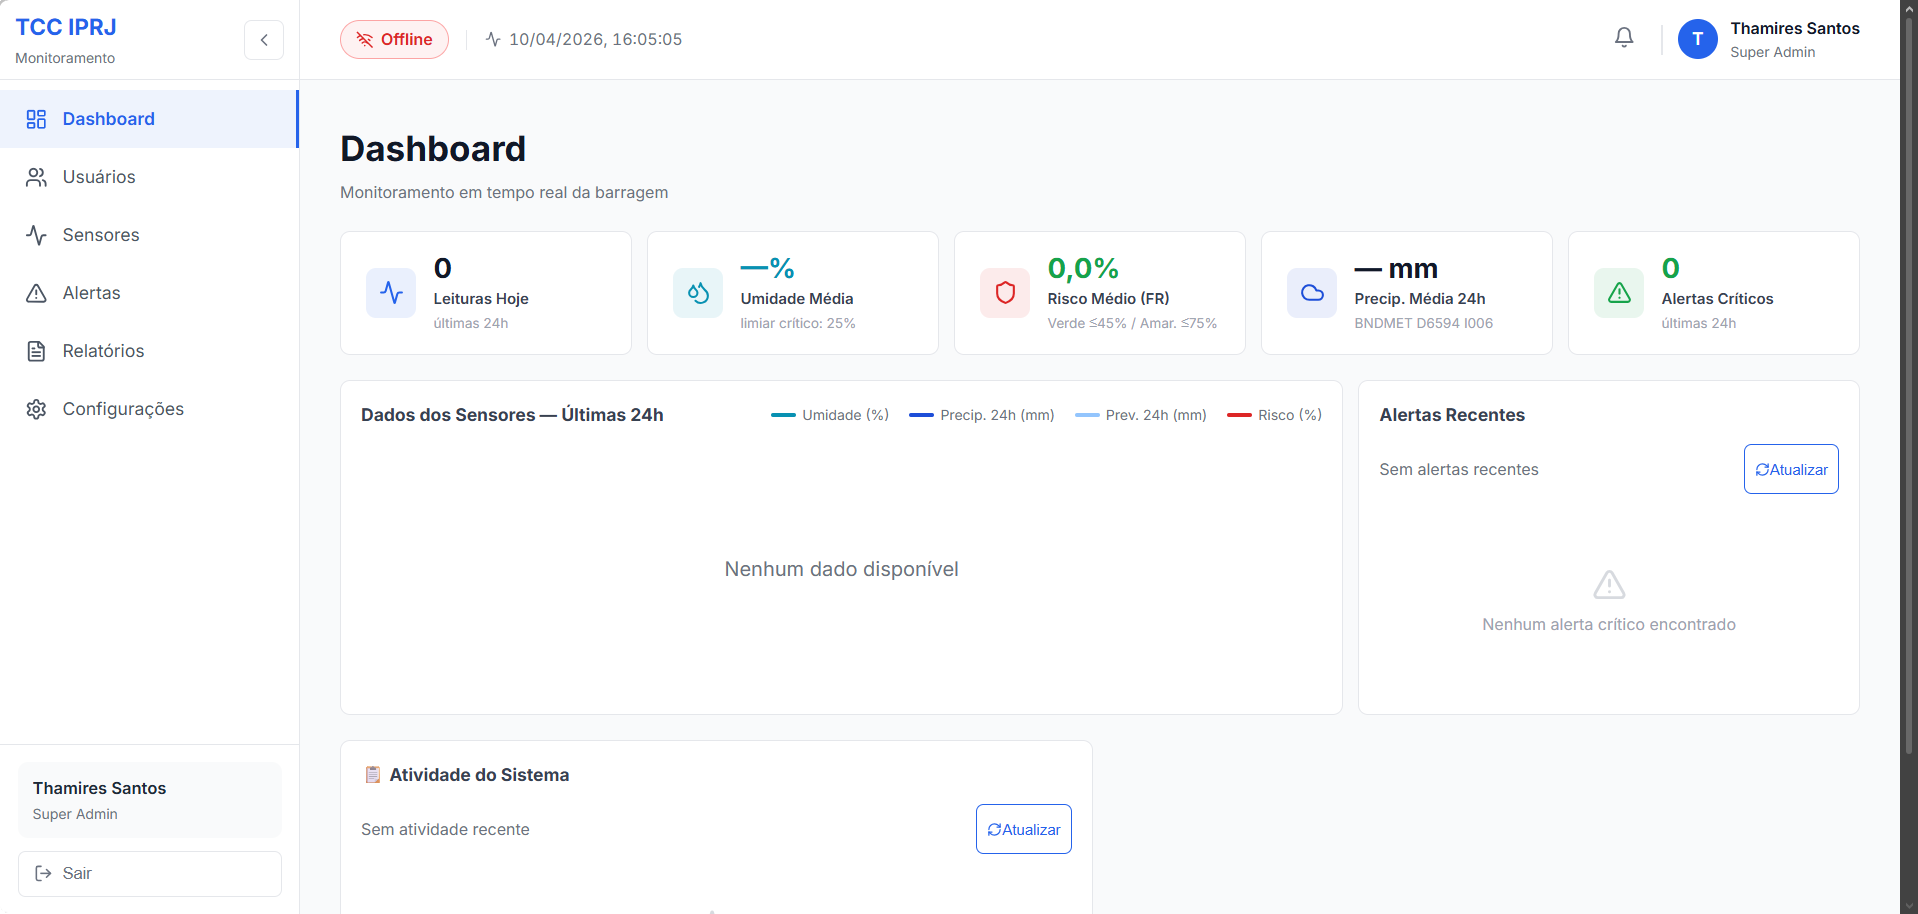
\includegraphics[width=0.95\textwidth]{figures/cap5_dashboard_indisponivel.png}
    \caption{\textit{Header} do \textit{dashboard} com status ``Offline''
    em vermelho: \textit{backend} inacessível, verificação de saúde sem
    resposta e sistema incapaz de receber ou exibir novos dados.}
    \label{fig:dashboard_indisponivel}
    \fonte{Elaborado pela autora.}
\end{figure}

Falhas ao carregar as estatísticas fazem com que os KPIs sejam exibidos
com valor zero enquanto o sistema aguarda nova tentativa, conforme ilustra a \autoref{fig:dashboard_kpis_zerados}.

\begin{figure}[htbp]
    \centering
    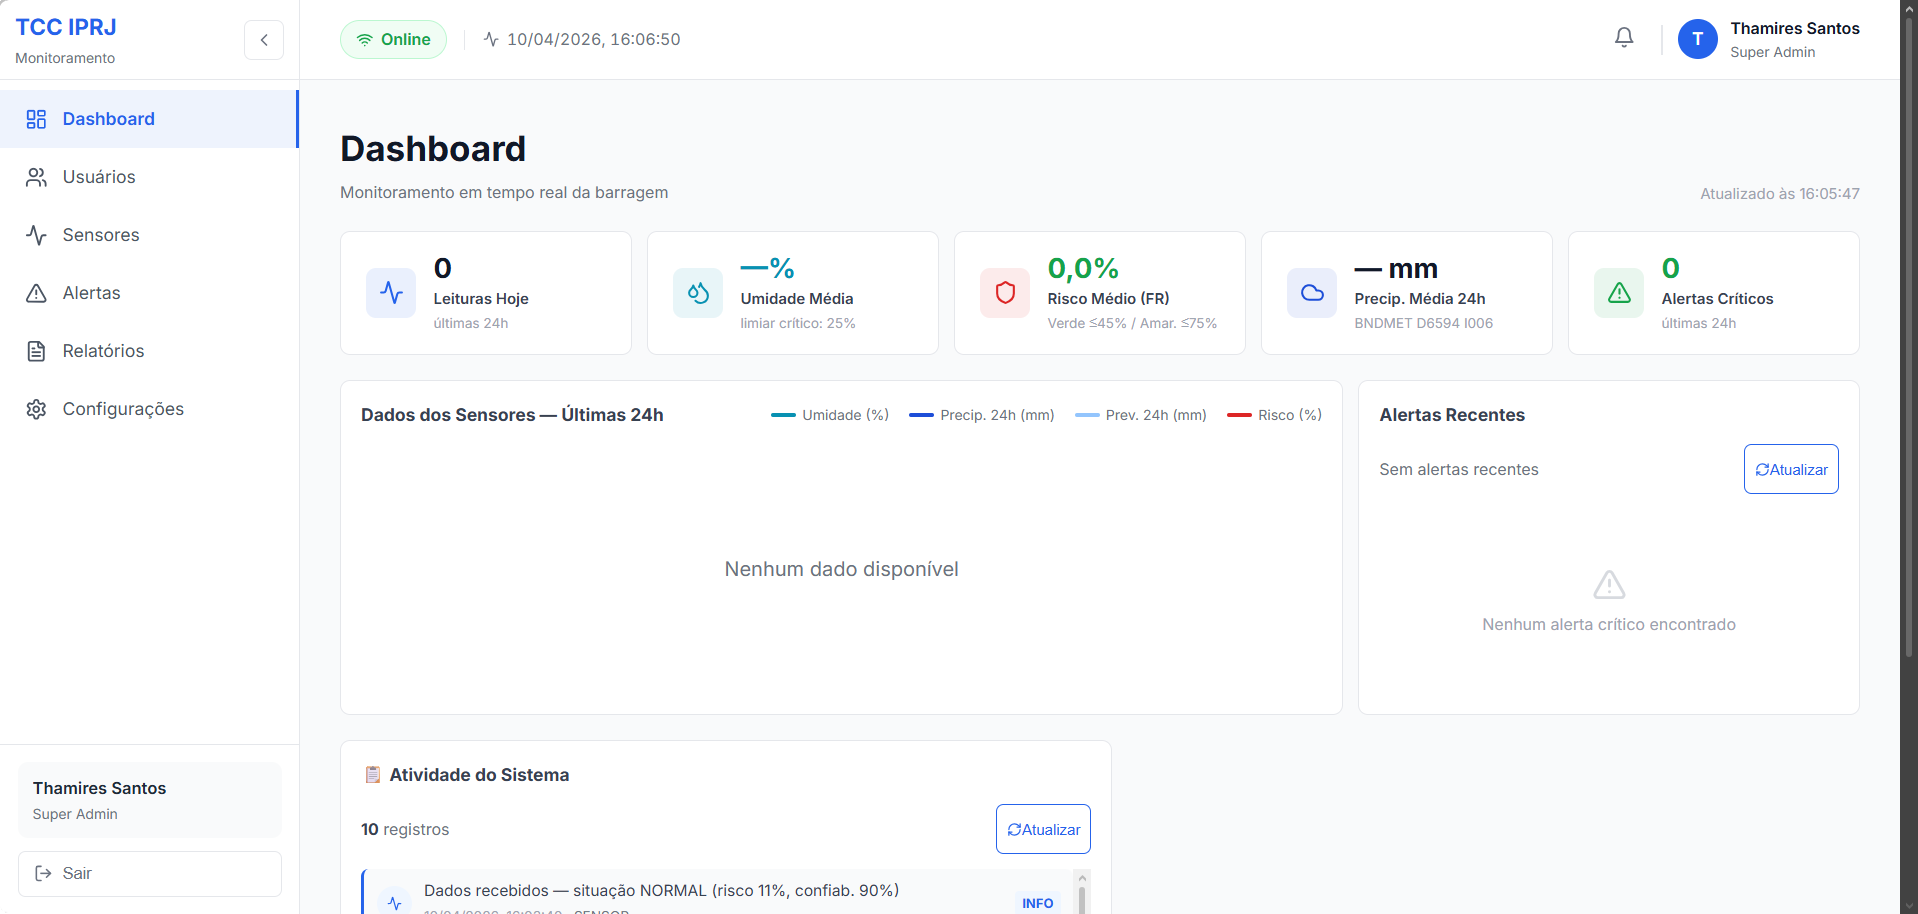
\includegraphics[width=0.95\textwidth]{figures/cap5_dashboard_kpis_zerados.png}
    \caption{\textit{Dashboard} com KPIs em valor zero por falha ao carregar estatísticas.}
    \label{fig:dashboard_kpis_zerados}
    \fonte{Elaborado pela autora.}
\end{figure}

% =============================================================
\section{Tela de Sensores e Histórico}
\label{sec:sensores}
% =============================================================

% -------------------------------------------------------------
\subsection{Carregamento Inicial e Período Padrão}
\label{subsec:sensores-inicial}
% -------------------------------------------------------------

A tela de Sensores apresenta ao administrador o histórico completo e
filtrável das leituras do sistema. Ao ser aberta, ela carrega
automaticamente as leituras das últimas 24 horas na tabela paginada,
acompanhadas dos KPIs calculados para esse período e do gráfico
histórico. As \autoref{fig:sensores_tabela_pt1} a
\autoref{fig:sensores_tabela_pt4} exibem essa configuração
inicial, com a tabela mostrando 15 registros por página, cada um com
\textit{timestamp}, umidade, valor ADC, índice de risco, nível de
alerta --- representado por um \textit{badge} colorido --- e status
das APIs e do sensor.

\begin{figure}[htbp]
    \centering
    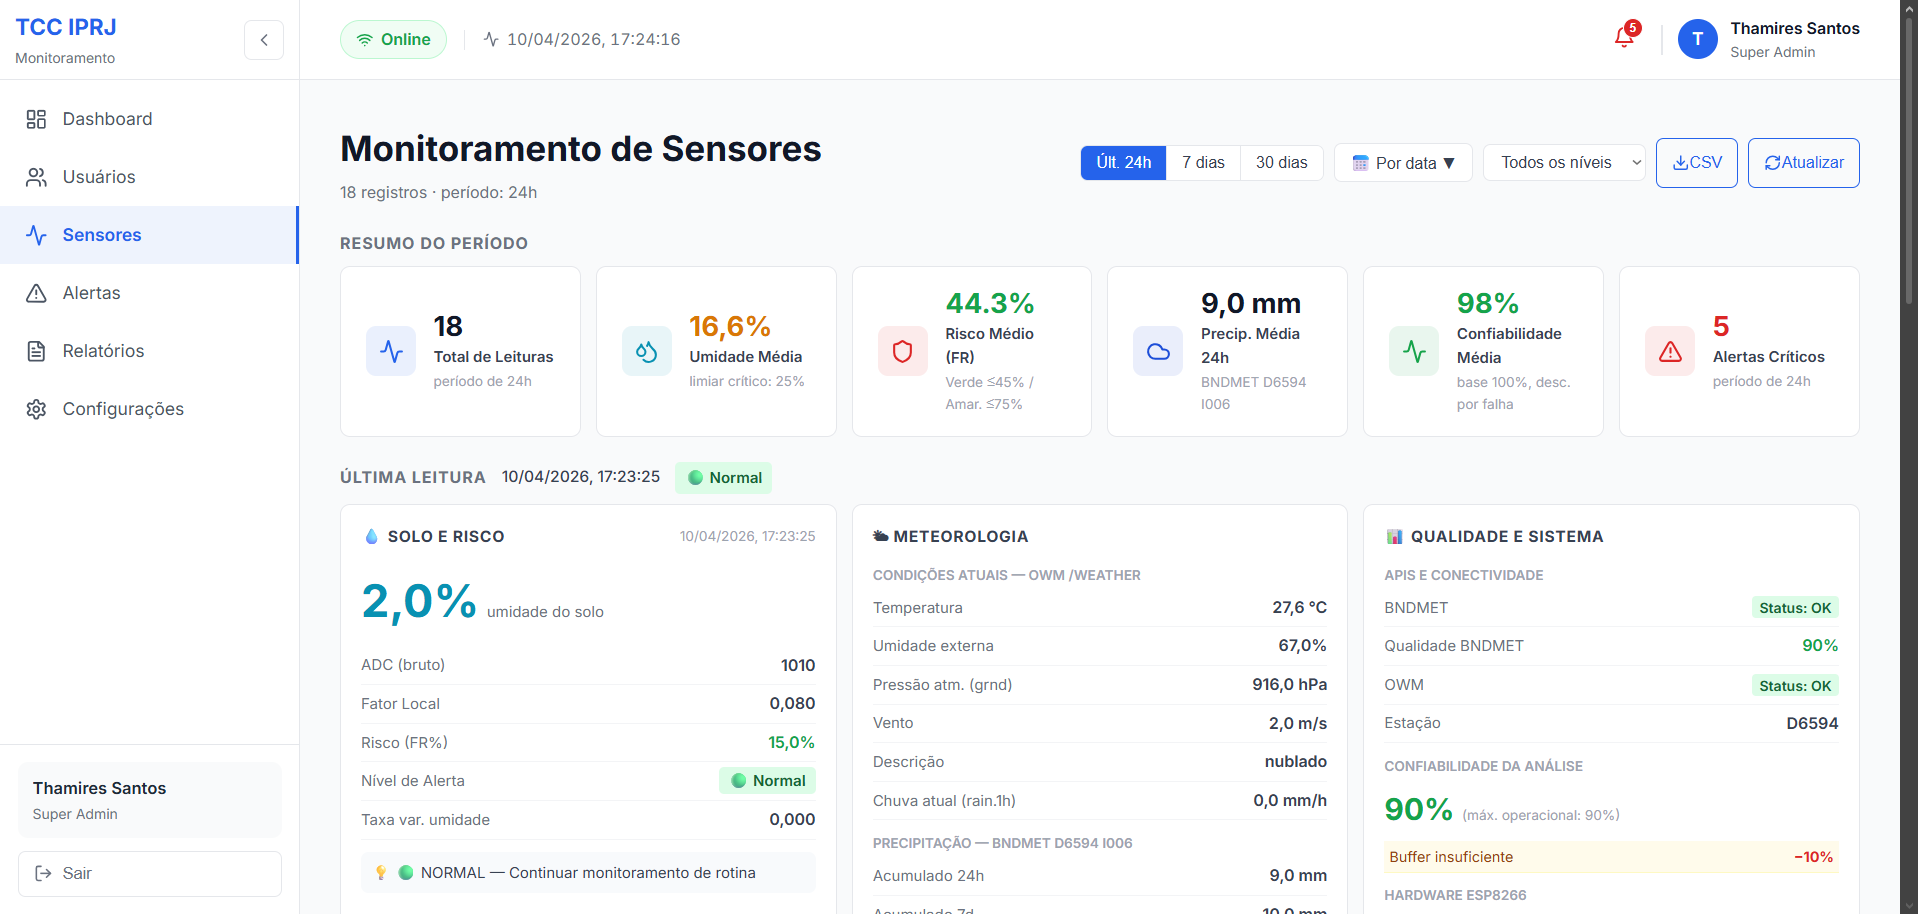
\includegraphics[width=0.95\textwidth]{figures/cap5_sensores_tabela_pt1.png}
    \caption{Tela de Sensores com período padrão de 24 horas (parte~1):
    KPIs do período, dados da última leitura, e filtros de período fixo e customizado disponíveis na interface.}
    \label{fig:sensores_tabela_pt1}
    \fonte{Elaborado pela autora.}
\end{figure}

\begin{figure}[htbp]
    \centering
    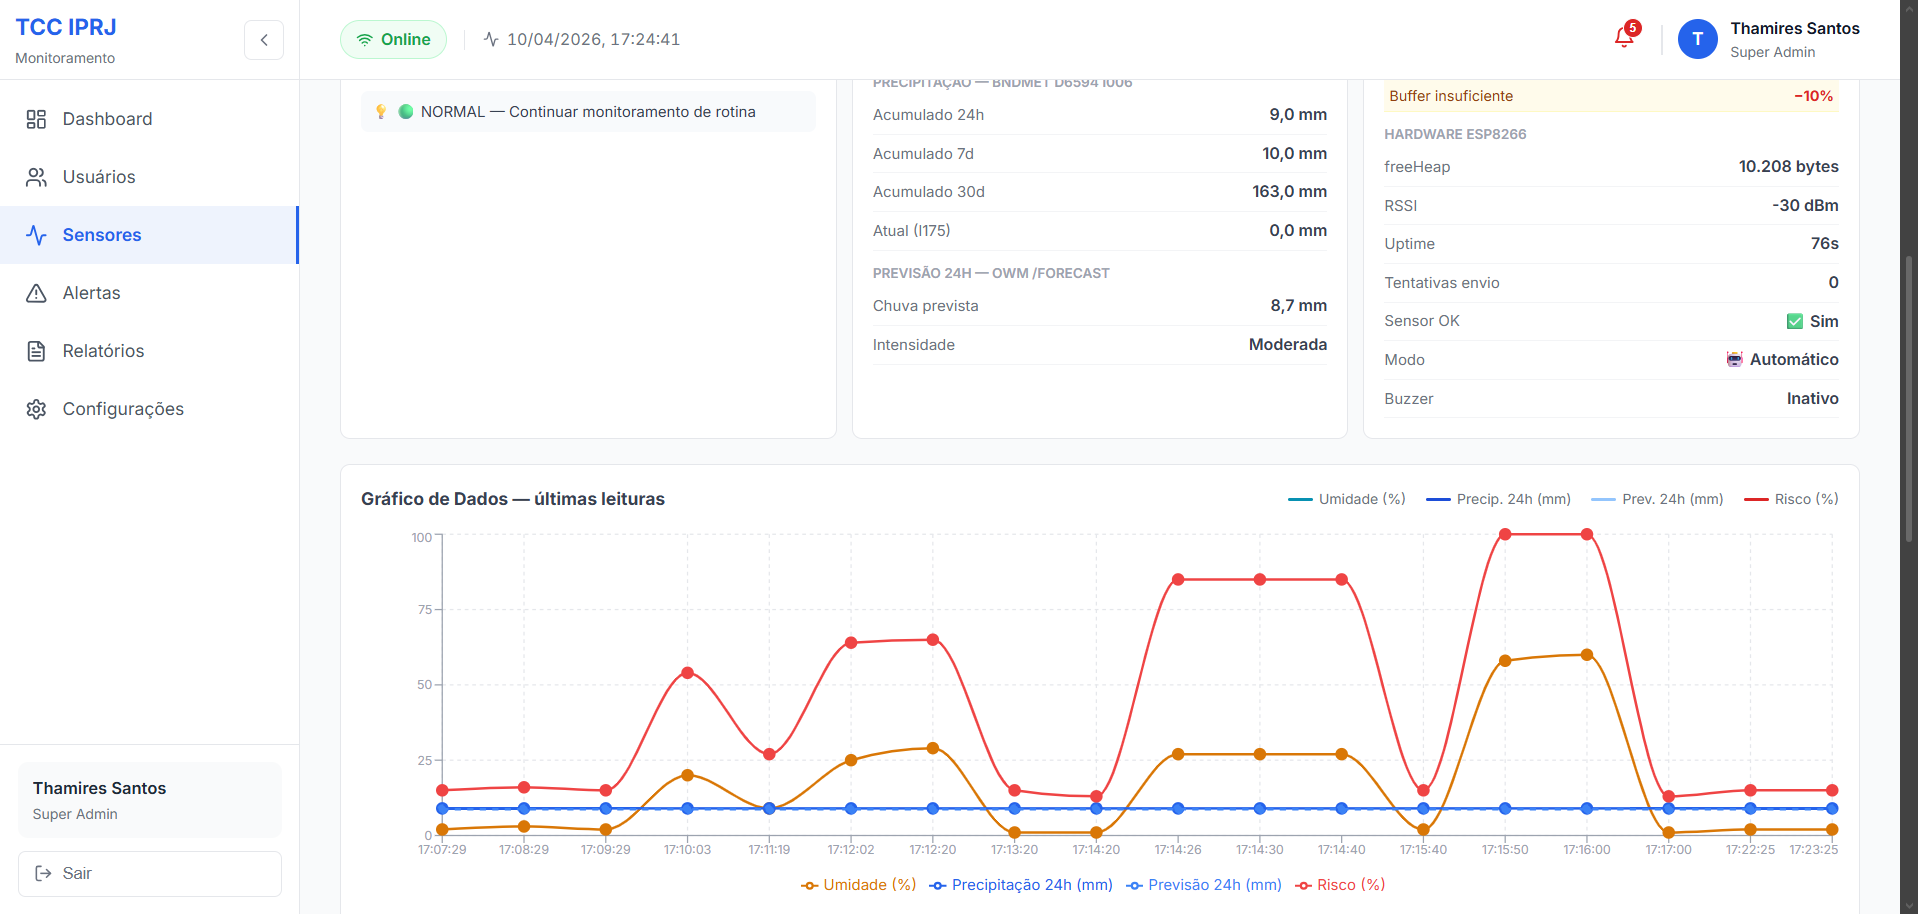
\includegraphics[width=0.95\textwidth]{figures/cap5_sensores_tabela_pt2.png}
    \caption{Tela de Sensores com período padrão de 24 horas (parte~2):
    gráfico histórico das séries de umidade, precipitação e risco.}
    \label{fig:sensores_tabela_pt2}
    \fonte{Elaborado pela autora.}
\end{figure}

\begin{figure}[htbp]
    \centering
    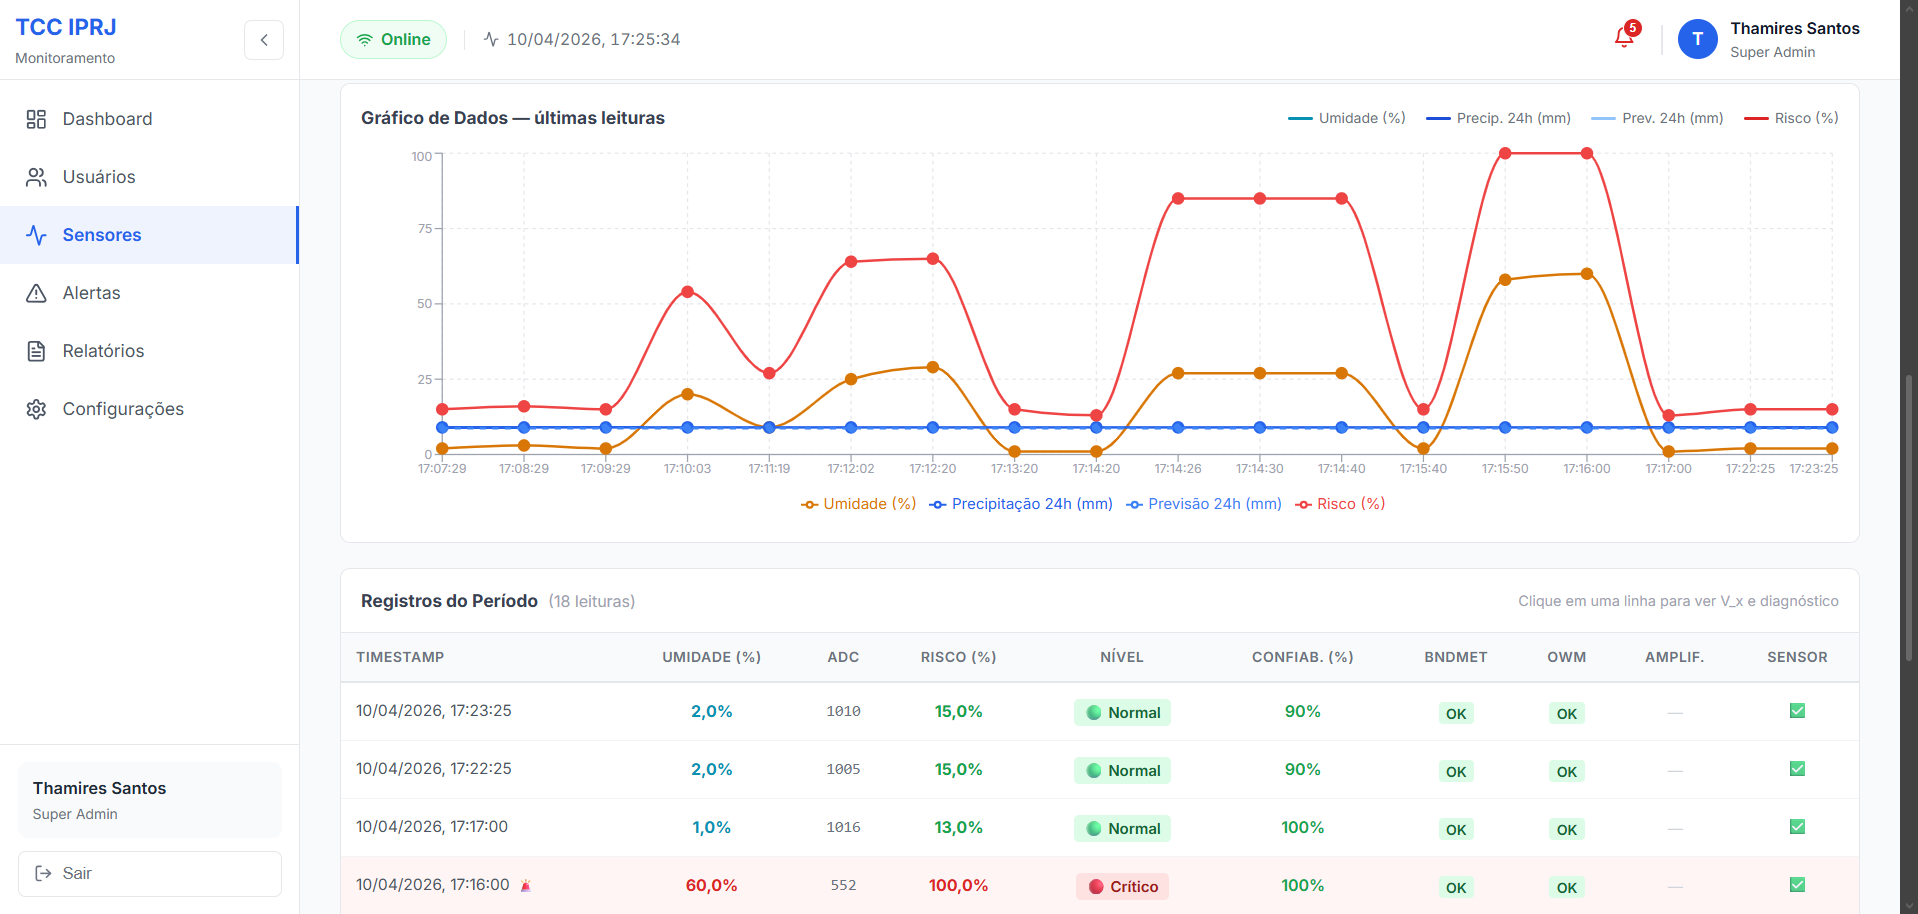
\includegraphics[width=0.95\textwidth]{figures/cap5_sensores_tabela_pt3.png}
    \caption{Tela de Sensores com período padrão de 24 horas (parte~3):
    início da tabela paginada com \textit{badges} de nível de alerta.}
    \label{fig:sensores_tabela_pt3}
    \fonte{Elaborado pela autora.}
\end{figure}

\begin{figure}[htbp]
    \centering
    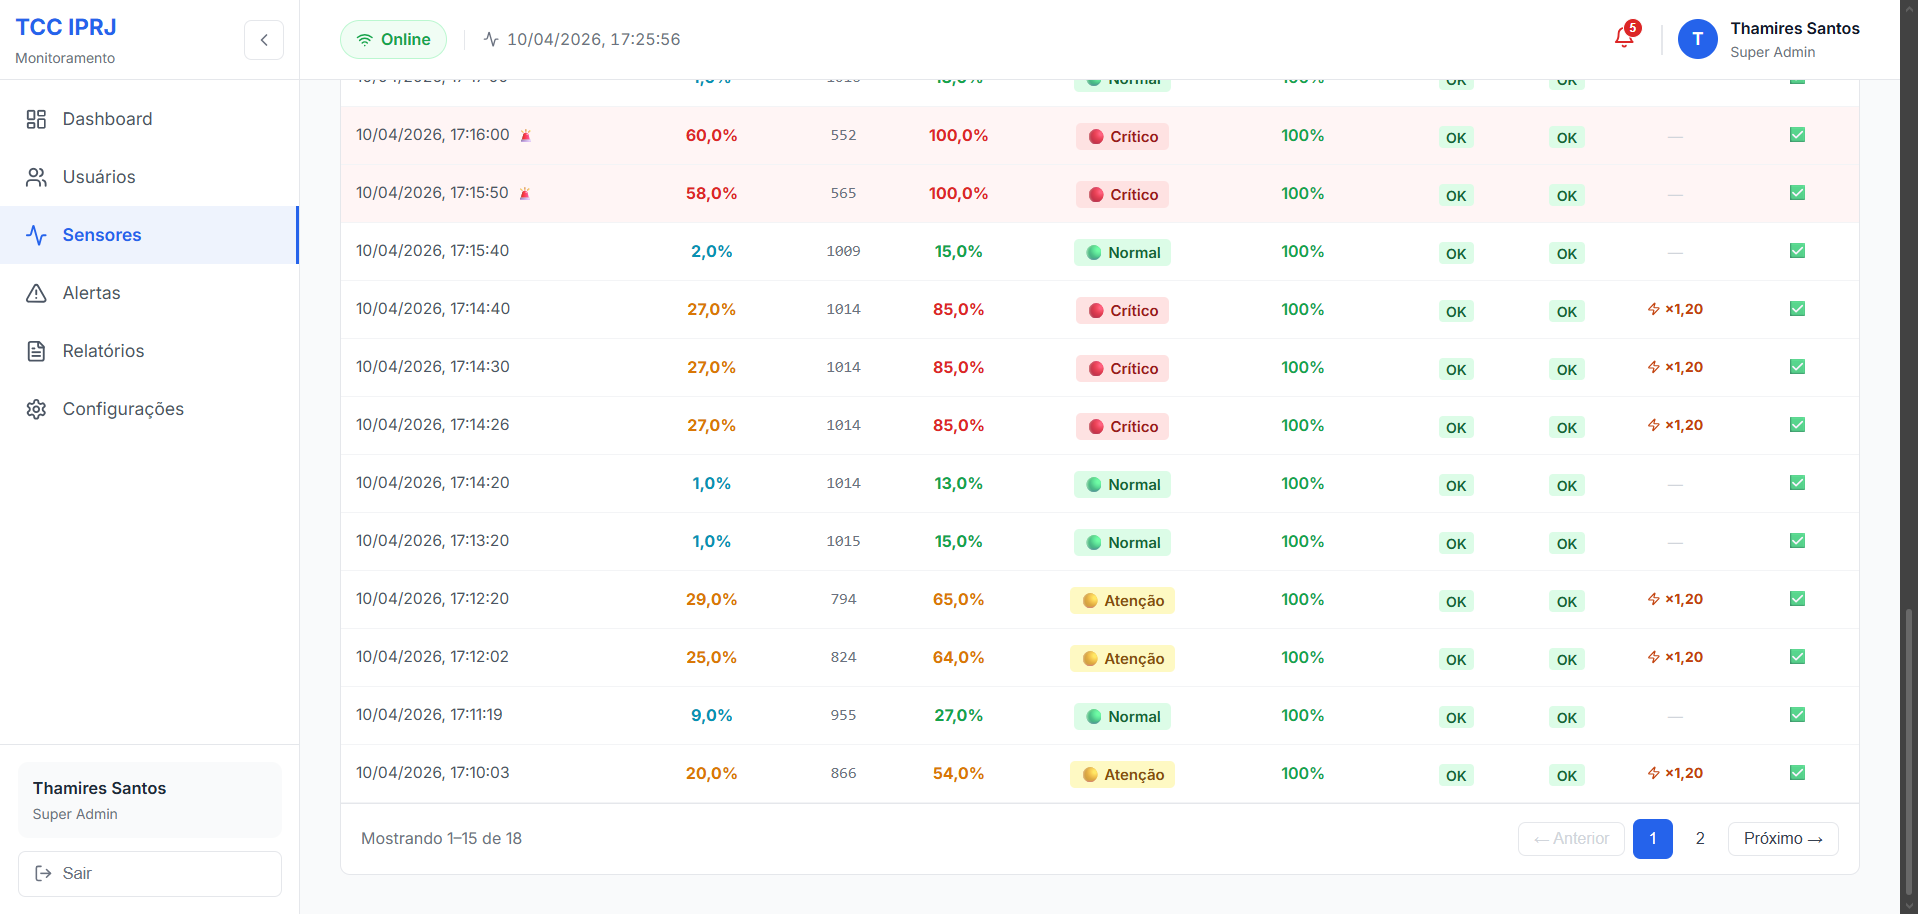
\includegraphics[width=0.95\textwidth]{figures/cap5_sensores_tabela_pt4.png}
    \caption{Tela de Sensores com período padrão de 24 horas (parte~4):
    continuação da tabela paginada com registros de leituras.}
    \label{fig:sensores_tabela_pt4}
    \fonte{Elaborado pela autora.}
\end{figure}

Caso ocorra falha na comunicação com o \textit{backend} durante o
carregamento, o sistema exibe o \textit{toast} ``Erro ao carregar dados
dos sensores'' e mantém os dados zerados nos KPIs; na área de Gráfico de Daods, exibe o texto ``Nenhum dado disponível'' em tela, e na área Registros do Período, exibe o texto ``Nenhum dado para o período selecionado'' em tela, conforme ilustra a \autoref{fig:sensores_erro_carregamento}.

\begin{figure}[htbp]
    \centering
    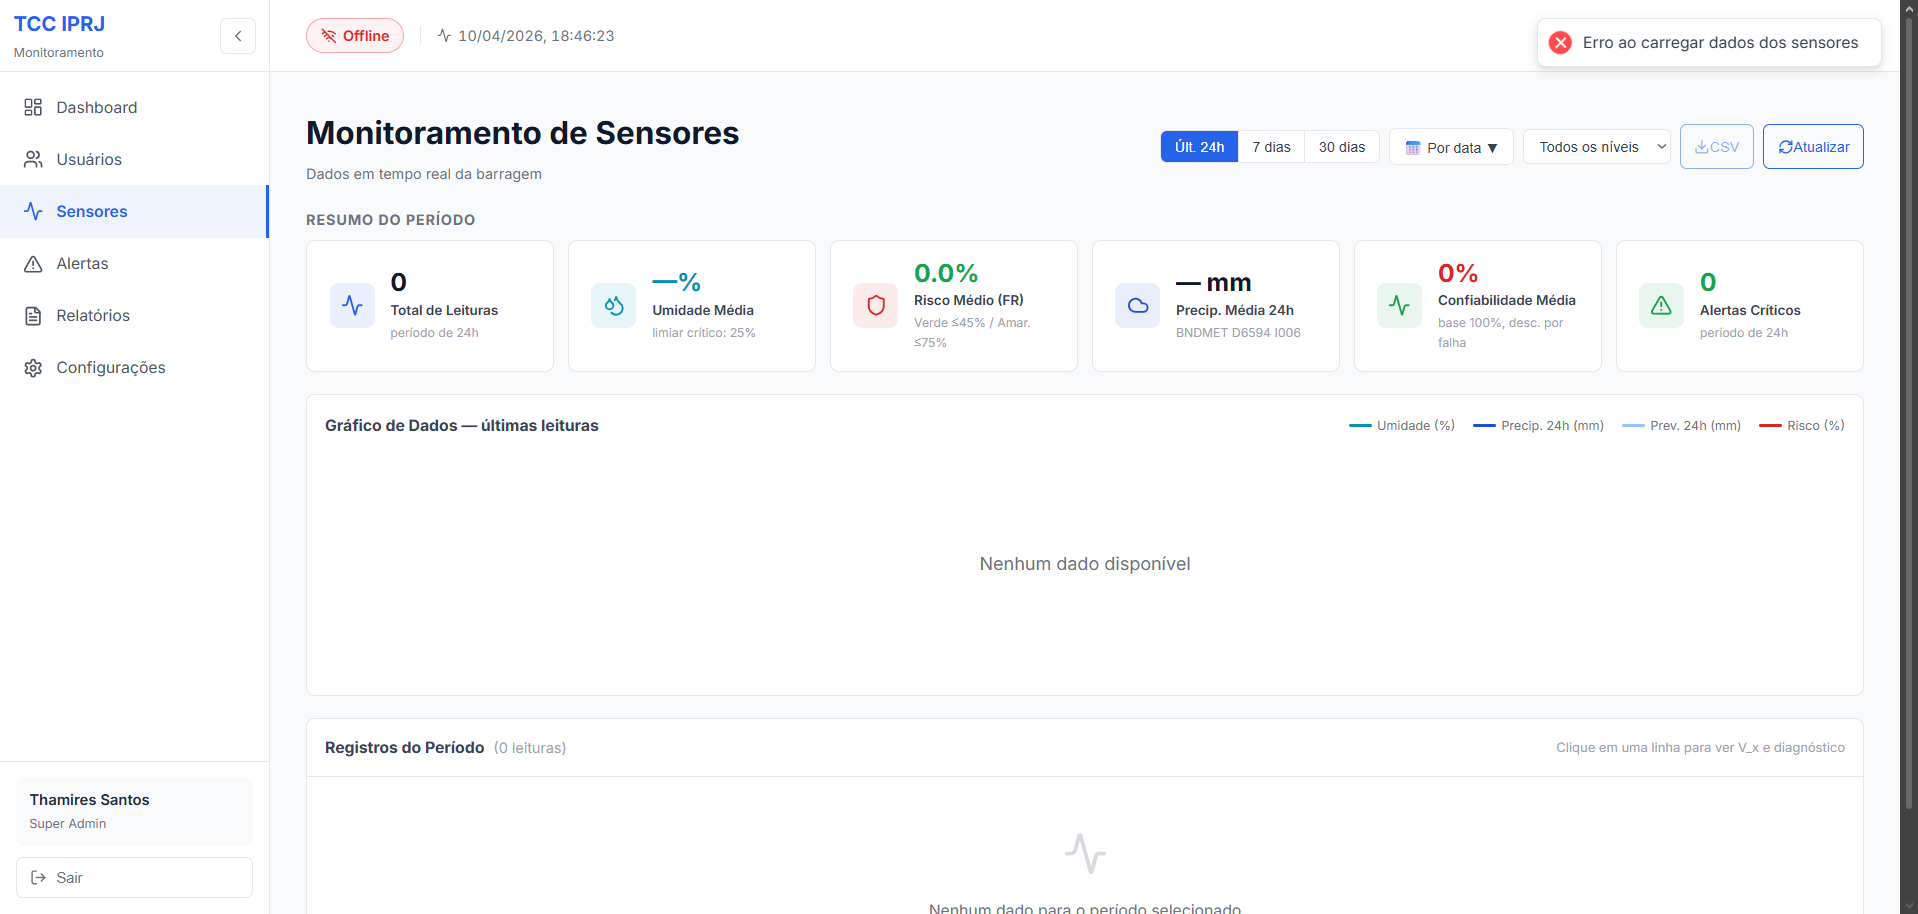
\includegraphics[width=0.95\textwidth]{figures/cap5_sensores_erro_carregamento.png}
    \caption{Tela de Sensores com \textit{toast} de erro ao carregar dados: falha na comunicação com o \textit{backend}.}
    \label{fig:sensores_erro_carregamento}
    \fonte{Elaborado pela autora.}
\end{figure}

% -------------------------------------------------------------
\subsection{Seleção de Período e Filtros}
\label{subsec:sensores-filtros}
% -------------------------------------------------------------

A \autoref{fig:sensores_tabela_pt1} exibe o estado inicial
da tela com o período padrão de 24 horas ativo e o botão
``Últimas 24h'' destacado. Três botões de período fixo
--- ``Últimas 24h'', ``7 dias'' e
``30 dias'' --- permitem alternar o intervalo de análise
com um clique. Ao selecionar um novo período, por exemplo em ``7 dias'', o botão anterior
perde o destaque, o botão selecionado passa a ser exibido em
azul e a tabela é recarregada com os dados do intervalo
escolhido e os KPIs recalculados, conforme ilustra a
\autoref{fig:sensores_periodo_fixo}.

Para intervalos específicos, o
filtro de período customizado aceita data e hora de início e de fim;
ao clicar em ``Aplicar'', os dados do intervalo definido são carregados, conforme ilustra a \autoref{fig:sensores_periodo_data}.

\begin{figure}[htbp]
    \centering
    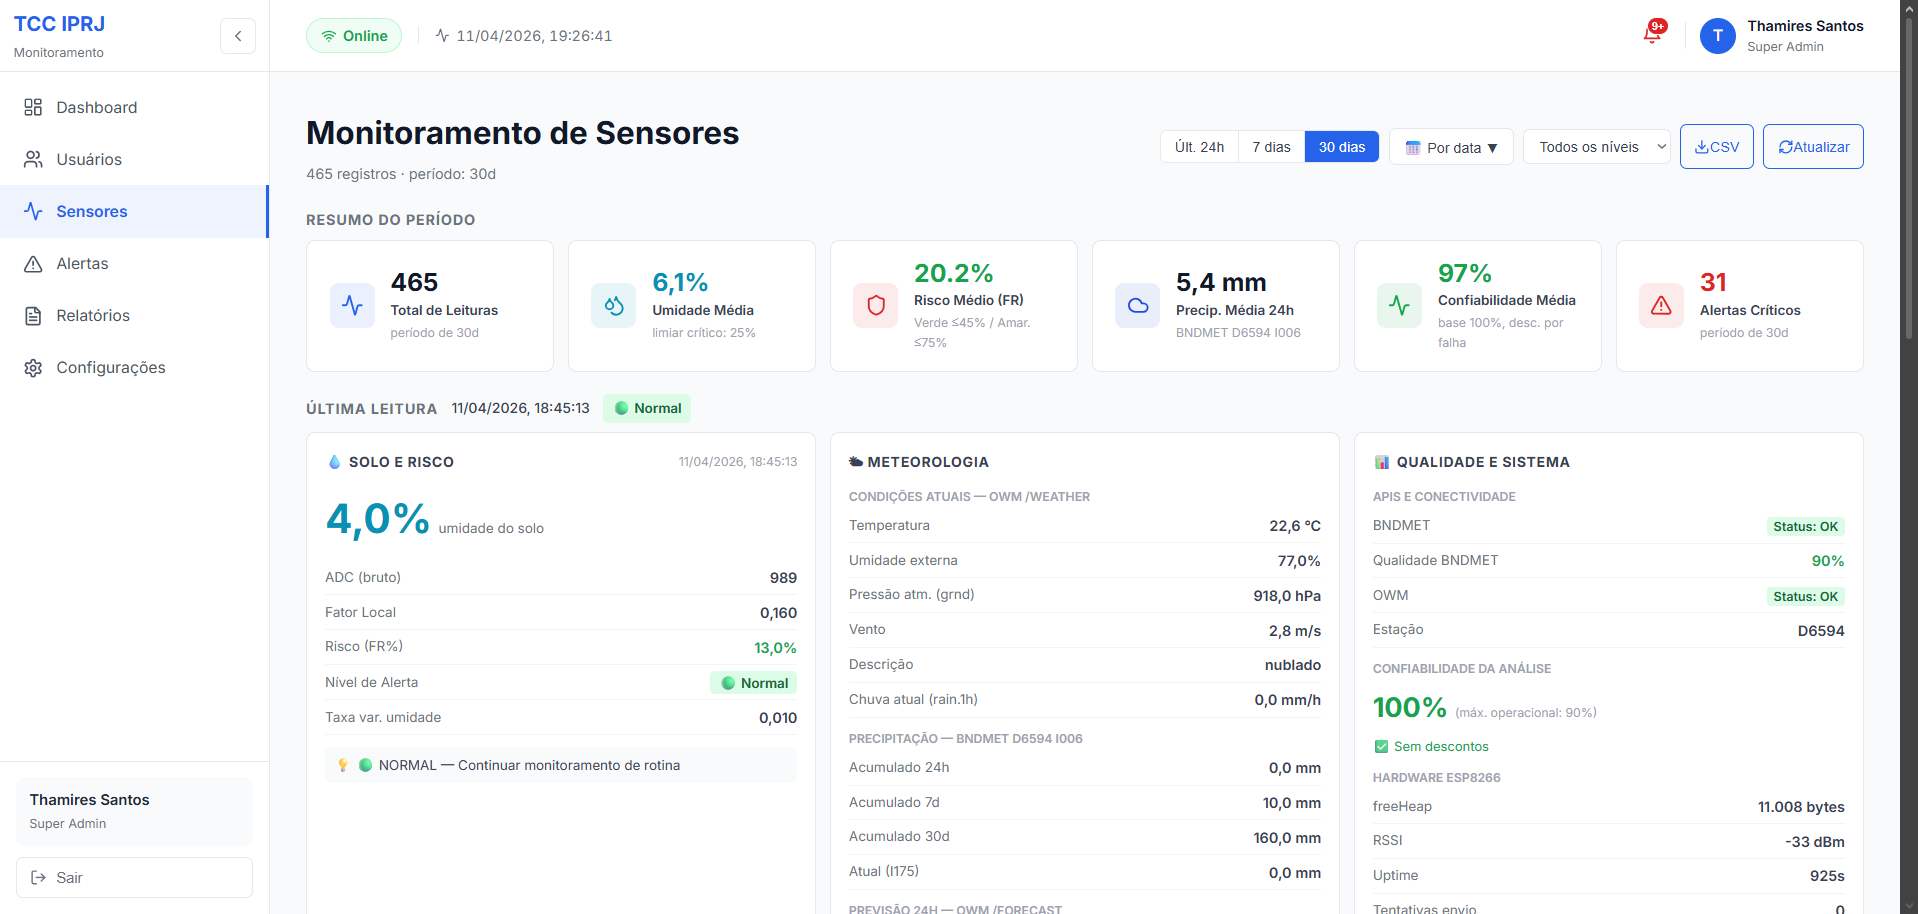
\includegraphics[width=0.95\textwidth]{figures/cap5_sensores_periodo_fixo.png}
    \caption{Tela de Sensores com período fixo: botão ativo fica destacado em azul e a tabela é recarregada com os dados do novo período.}
    \label{fig:sensores_periodo_fixo}
    \fonte{Elaborado pela autora.}
\end{figure}

\begin{figure}[htbp]
    \centering
    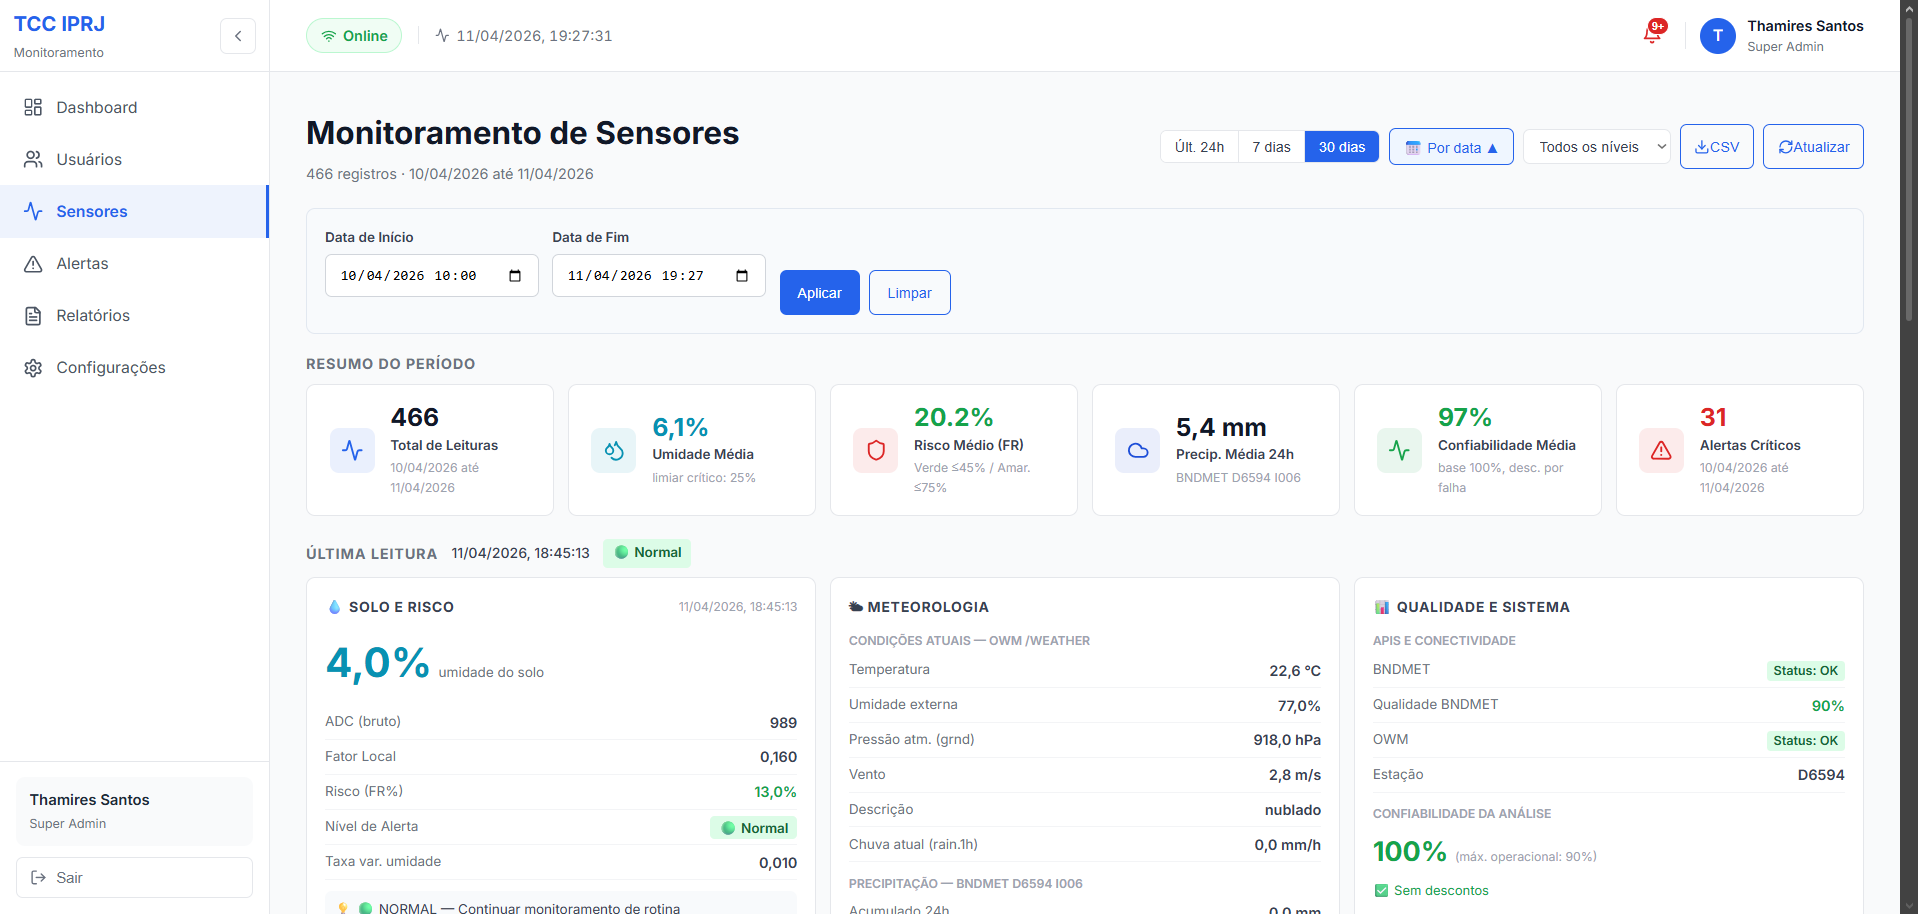
\includegraphics[width=0.95\textwidth]{figures/cap5_sensores_periodo_data.png}
    \caption{Tela de Sensores com período customizado: aceita data e hora de início e de fim.}
    \label{fig:sensores_periodo_data}
    \fonte{Elaborado pela autora.}
\end{figure}

Se as datas não forem preenchidas, o botão ``Aplicar'' fica desabilitado, conforme ilustra a \autoref{fig:sensores_filtro_datas_vazias};
se a data de início for posterior à data de fim, outro \textit{toast}
informa o erro sem executar a consulta, conforme ilustra a \autoref{fig:sensores_filtro_datas_invalidas}.

\begin{figure}[htbp]
    \centering
    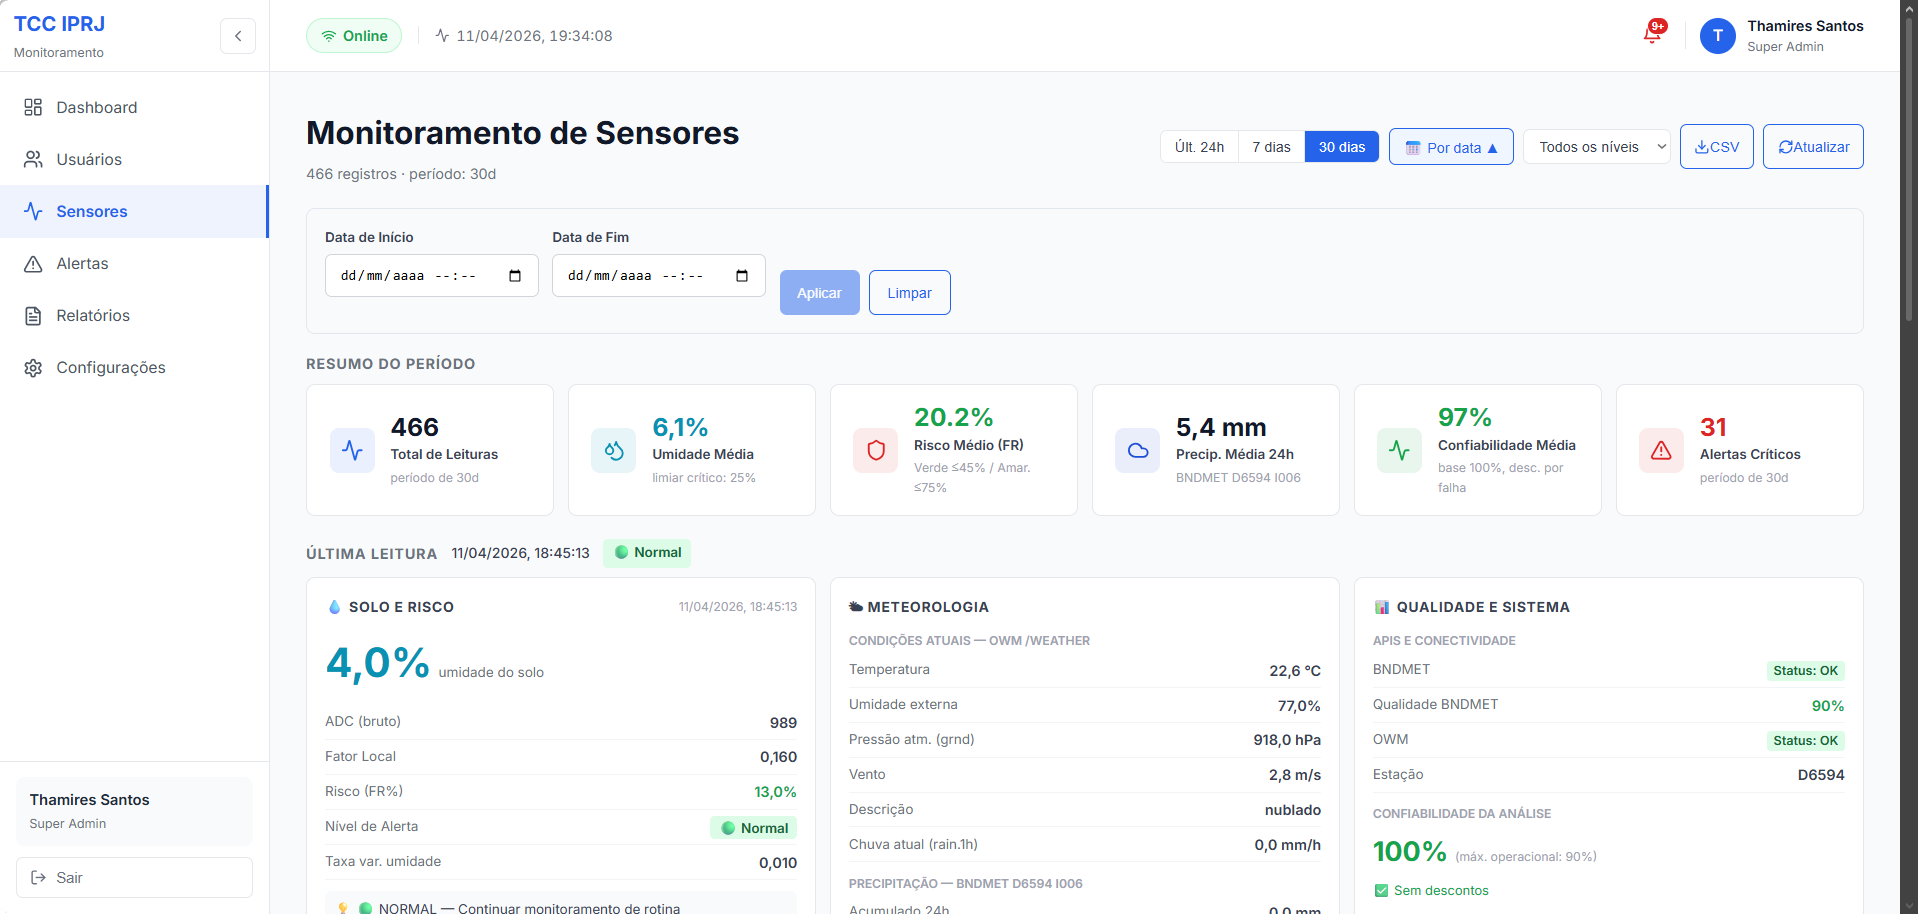
\includegraphics[width=0.95\textwidth]{figures/cap5_sensores_filtro_datas_vazias.png}
    \caption{Tela de Sensores com validação do filtro de período customizado: datas não preenchidas.}
    \label{fig:sensores_filtro_datas_vazias}
    \fonte{Elaborado pela autora.}
\end{figure}

\begin{figure}[htbp]
    \centering
    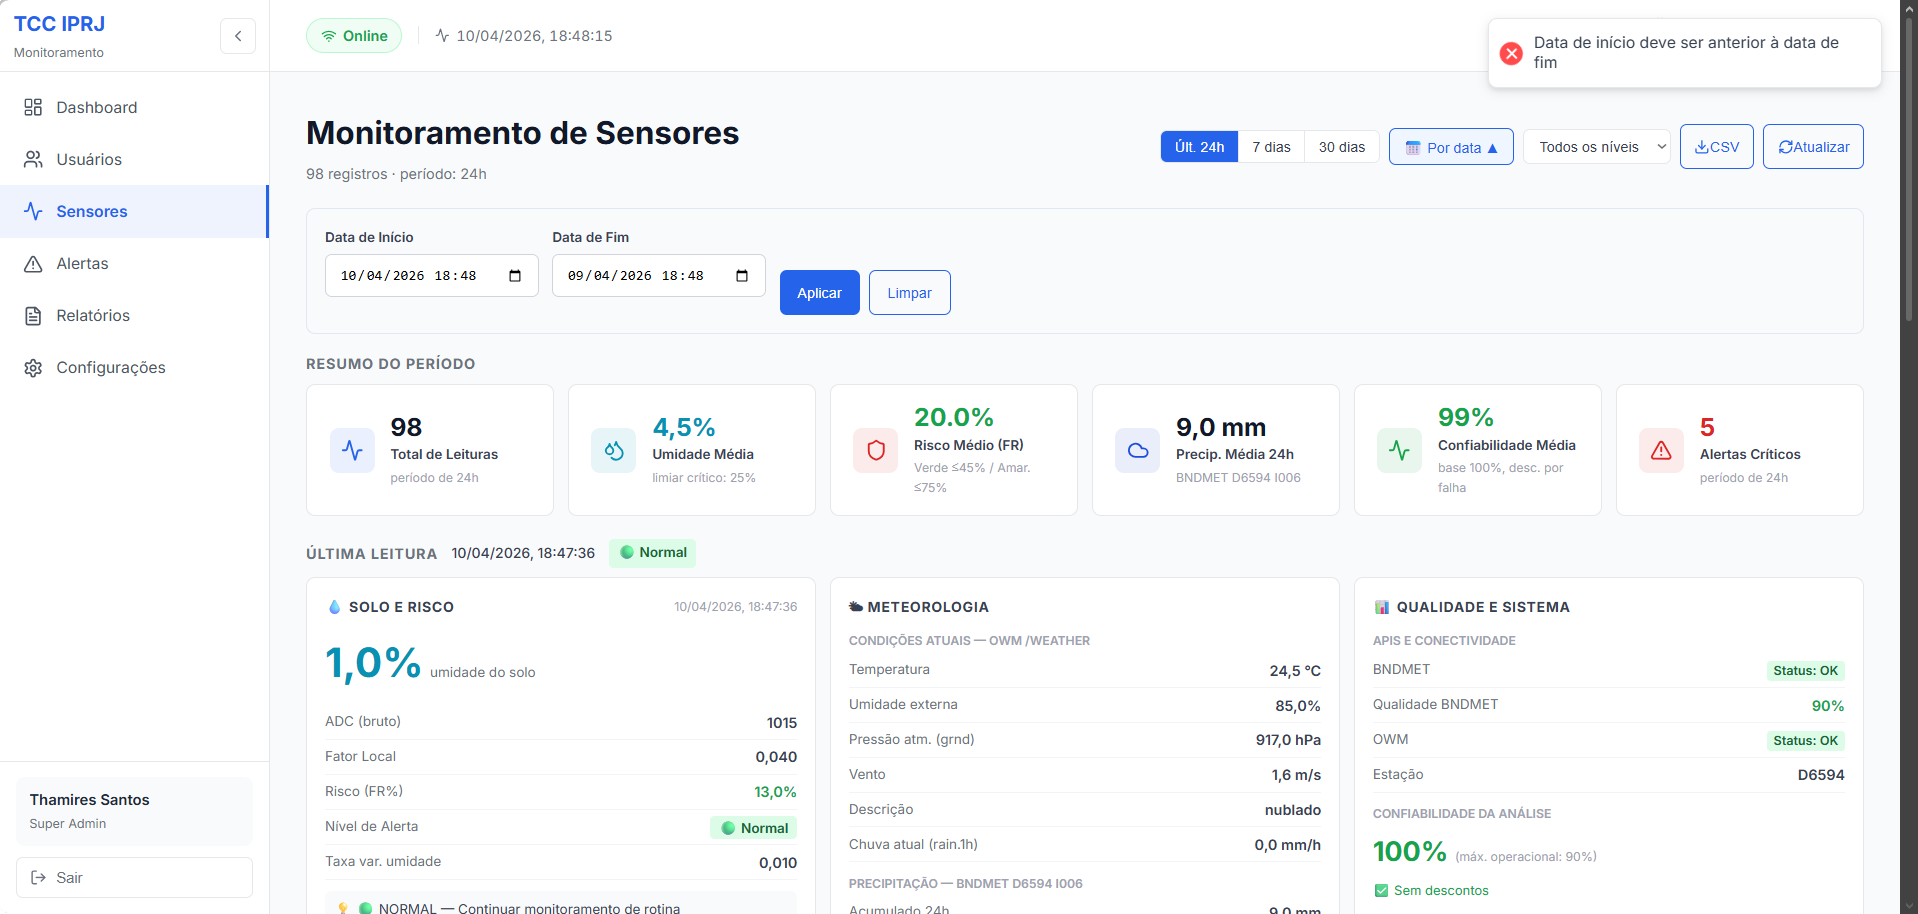
\includegraphics[width=0.95\textwidth]{figures/cap5_sensores_filtro_datas_invalidas.png}
    \caption{Tela de Sensores com validação do filtro de período customizado: \textit{toast} para data de início posterior à data de fim.}
    \label{fig:sensores_filtro_datas_invalidas}
    \fonte{Elaborado pela autora.}
\end{figure}

Um quinto filtro, por nível de alerta, é aplicado localmente sobre os
dados já carregados, sem nova chamada ao servidor. Ao selecioná-lo, a
tabela restringe a exibição às leituras do nível escolhido e a paginação
é recalculada, conforme ilustra as \autoref{fig:sensores_filtro_com_resultado_pt1} e \autoref{fig:sensores_filtro_com_resultado_pt2}. Quando nenhum registro corresponde ao filtro combinado de
período e nível, a tabela exibe estado vazio com mensagem informativa, conforme ilustra a \autoref{fig:sensores_filtro_sem_resultado}.

\begin{figure}[htbp]
    \centering
    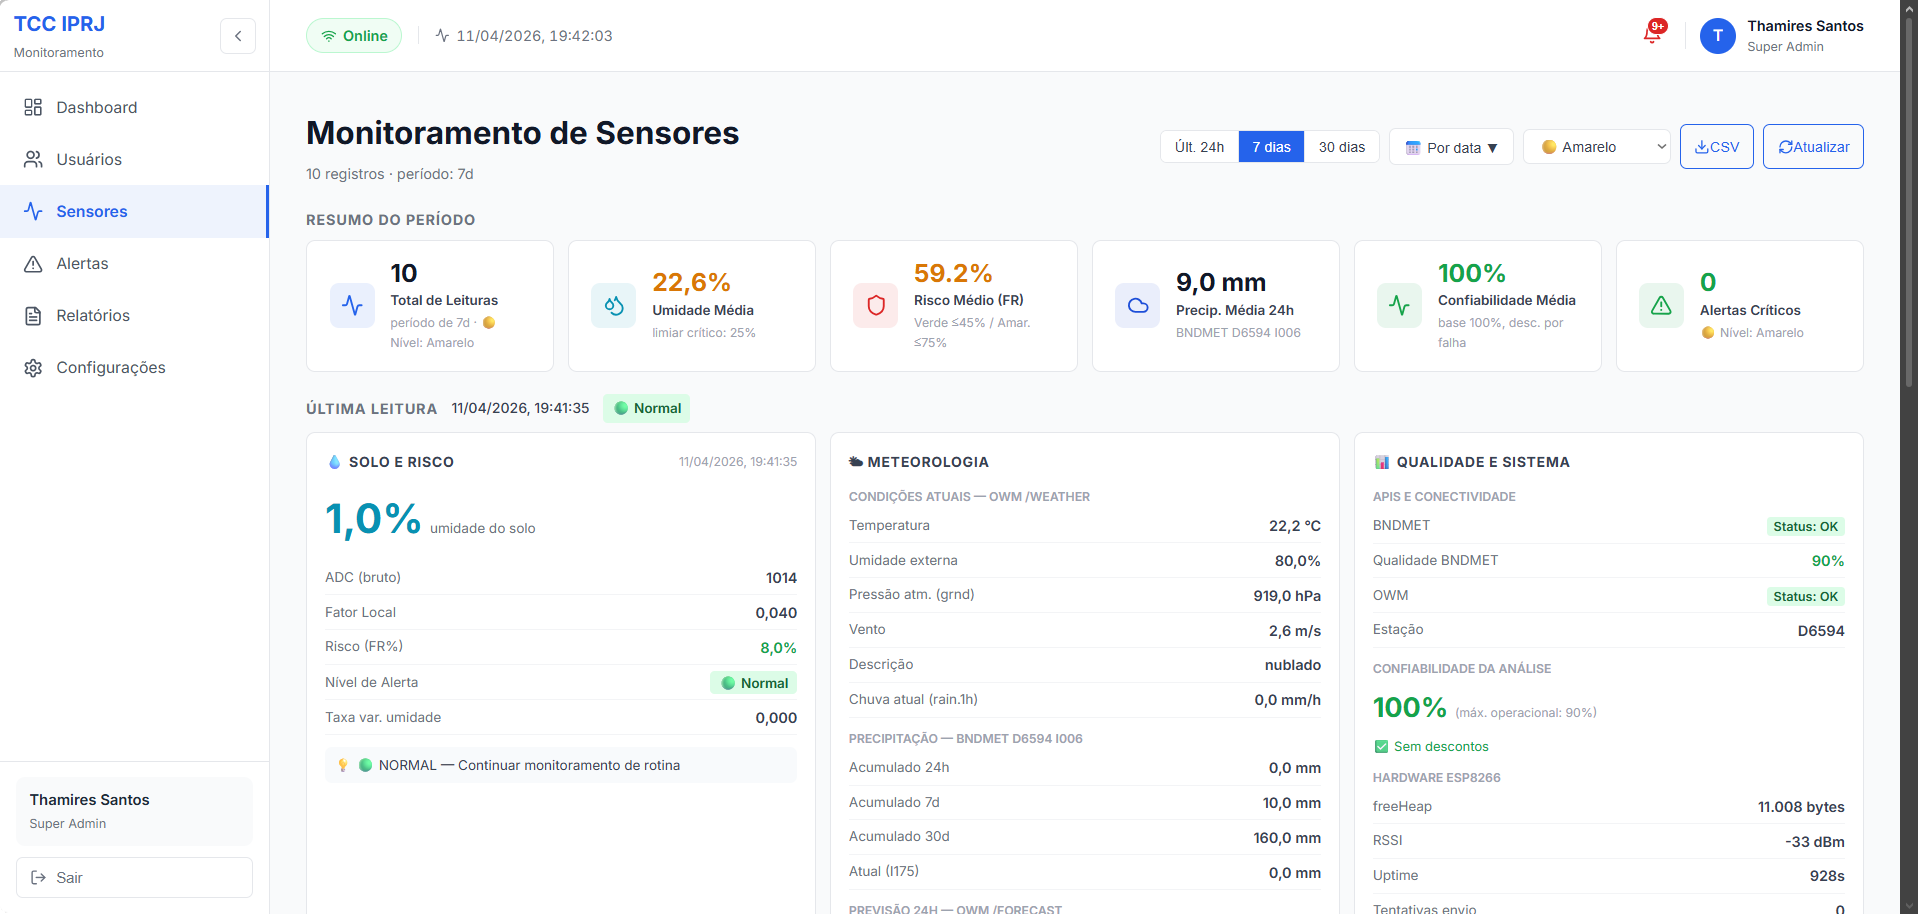
\includegraphics[width=0.95\textwidth]{figures/cap5_sensores_filtro_com_resultado_pt1.png}
    \caption{Tela de Sensores com filtro por nível de alerta (parte~1):
    KPIs calculados para o subconjunto filtrado e dados da última leitura.}
    \label{fig:sensores_filtro_com_resultado_pt1}
    \fonte{Elaborado pela autora.}
\end{figure}

\begin{figure}[htbp]
    \centering
    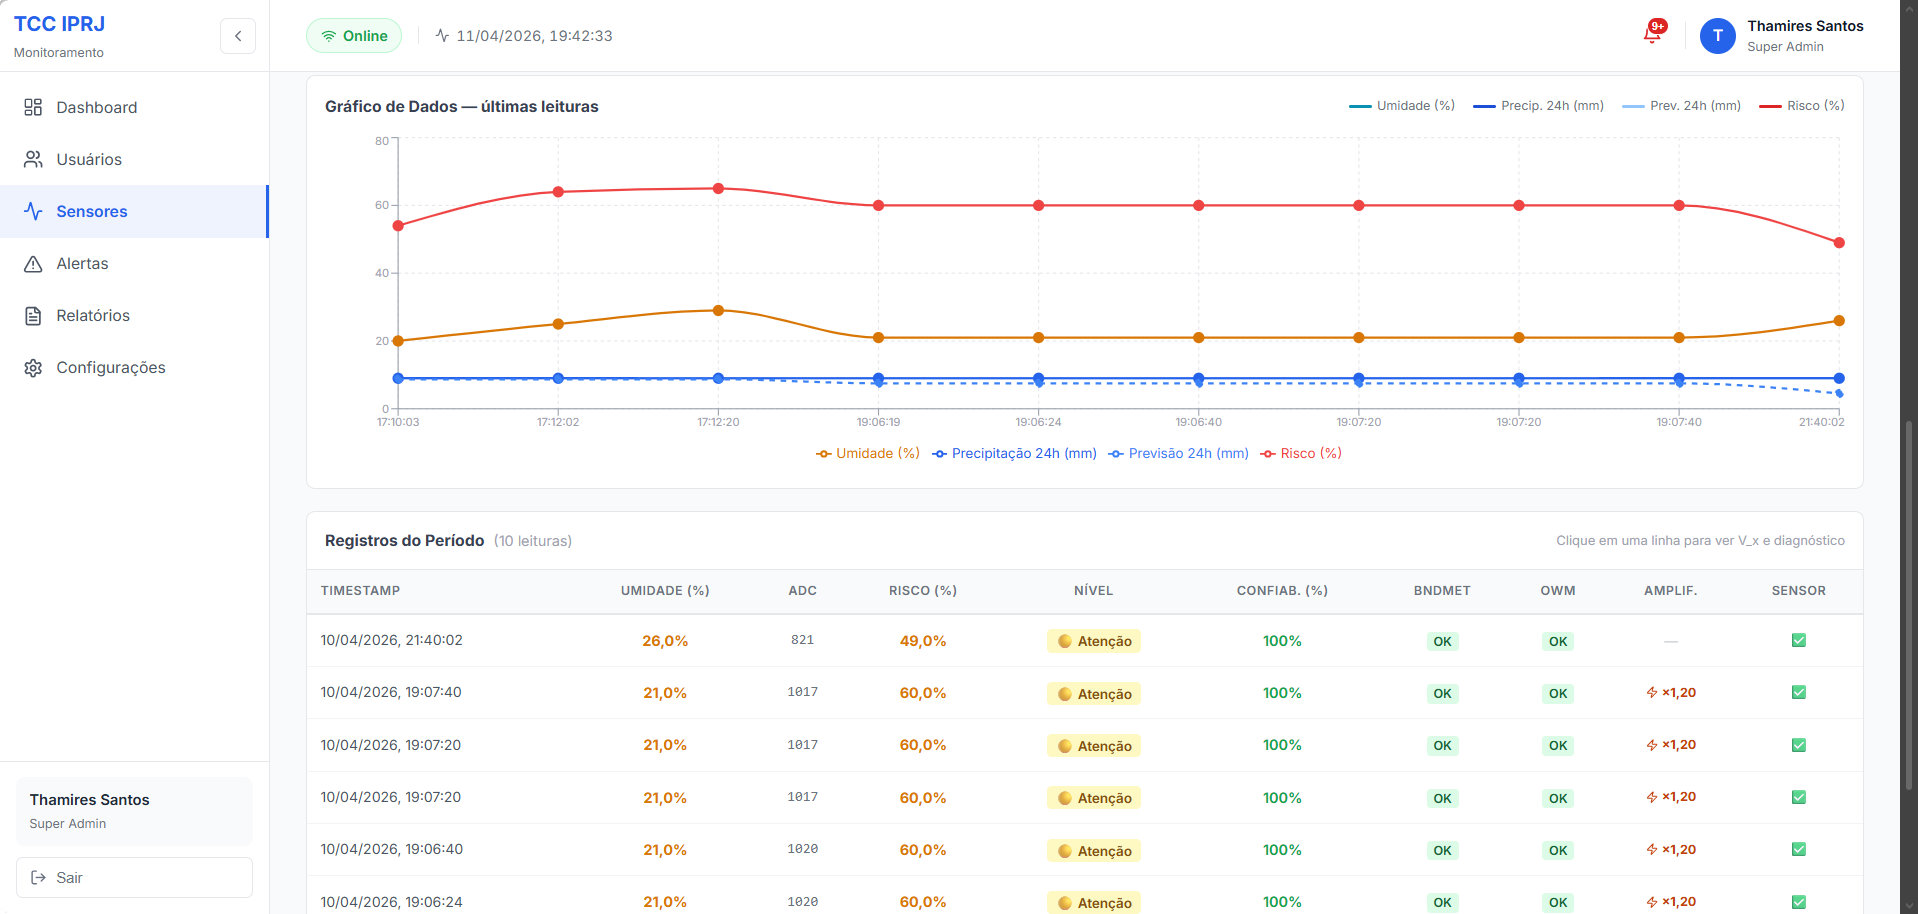
\includegraphics[width=0.95\textwidth]{figures/cap5_sensores_filtro_com_resultado_pt2.png}
    \caption{Tela de Sensores com filtro por nível de alerta (parte~2): tabela paginada com registros de leituras.}
    \label{fig:sensores_filtro_com_resultado_pt2}
    \fonte{Elaborado pela autora.}
\end{figure}

\begin{figure}[htbp]
    \centering
    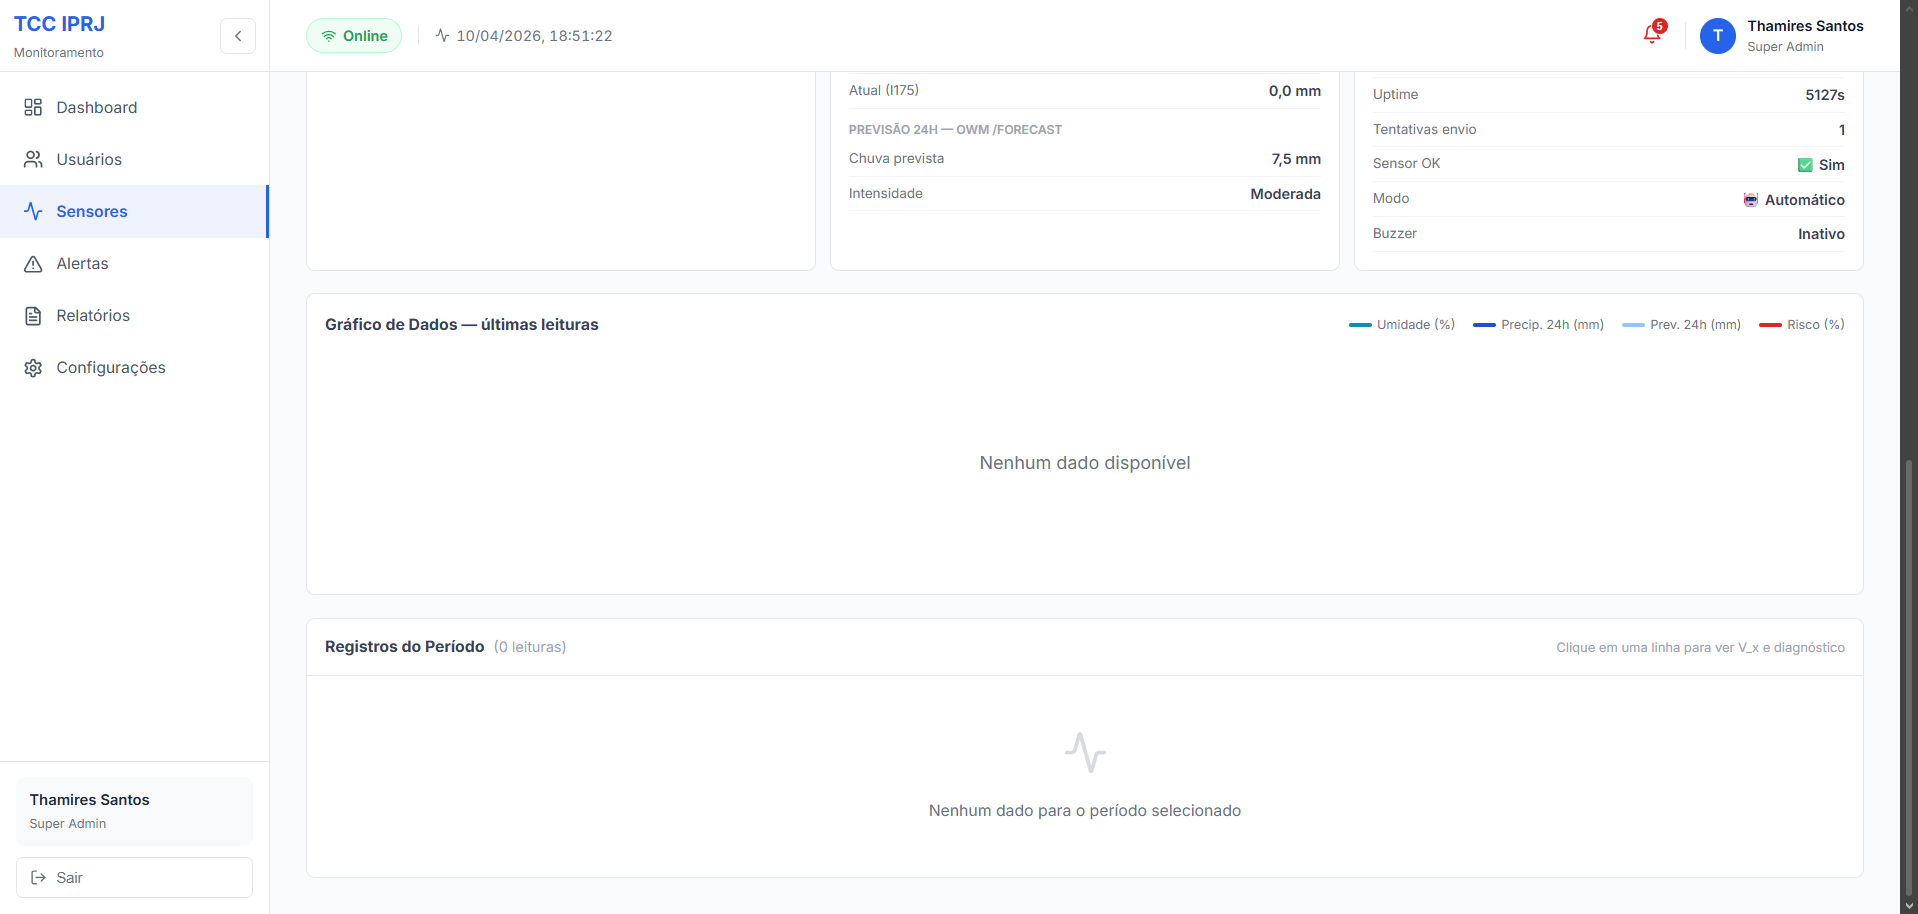
\includegraphics[width=0.95\textwidth]{figures/cap5_sensores_filtro_sem_resultado.png}
    \caption{Tela de Sensores com filtro por nível de alerta sem registros correspondentes: tabela em estado vazio com mensagem informativa e KPIs zerados para o subconjunto filtrado.}
    \label{fig:sensores_filtro_sem_resultado}
    \fonte{Elaborado pela autora.}
\end{figure}

% -------------------------------------------------------------
\subsection{Detalhamento de Leitura}
\label{subsec:sensores-detalhe}
% -------------------------------------------------------------

Cada linha da tabela pode ser expandida ao clicar sobre ela, revelando
quatro blocos de informação. O primeiro bloco exibe os sete
componentes individuais do modelo de risco com três casas decimais e a
soma do fator integrado.
O segundo apresenta o contexto meteorológico
completo: precipitações acumuladas nas três janelas temporais, previsão
de 24 horas com a classificação de intensidade, temperatura, umidade
relativa do ar, pressão atmosférica e descrição textual das condições.
O terceiro bloco traz o diagnóstico de \textit{hardware}: memória livre
em bytes, intensidade do sinal Wi-Fi em dBm, tempo de operação desde o
último \textit{boot}, tentativas de envio e estado do \textit{buzzer}.
O quarto bloco exibe a recomendação operacional gerada pelo dispositivo. 
Os níveis ``Normal'' e ``Atenção'' são
exibidos conforme ilustram as \autoref{fig:sensores_expandido_pt1} e \autoref{fig:sensores_expandido_pt2}, respectivamente; já 
os níveis ``Crítico'' e ``Ruptura'' são ilustrados como ilustram as \autoref{fig:sensores_expandido_pt3} e \autoref{fig:sensores_expandido_pt4}, nesta ordem.

\begin{figure}[htbp]
    \centering
    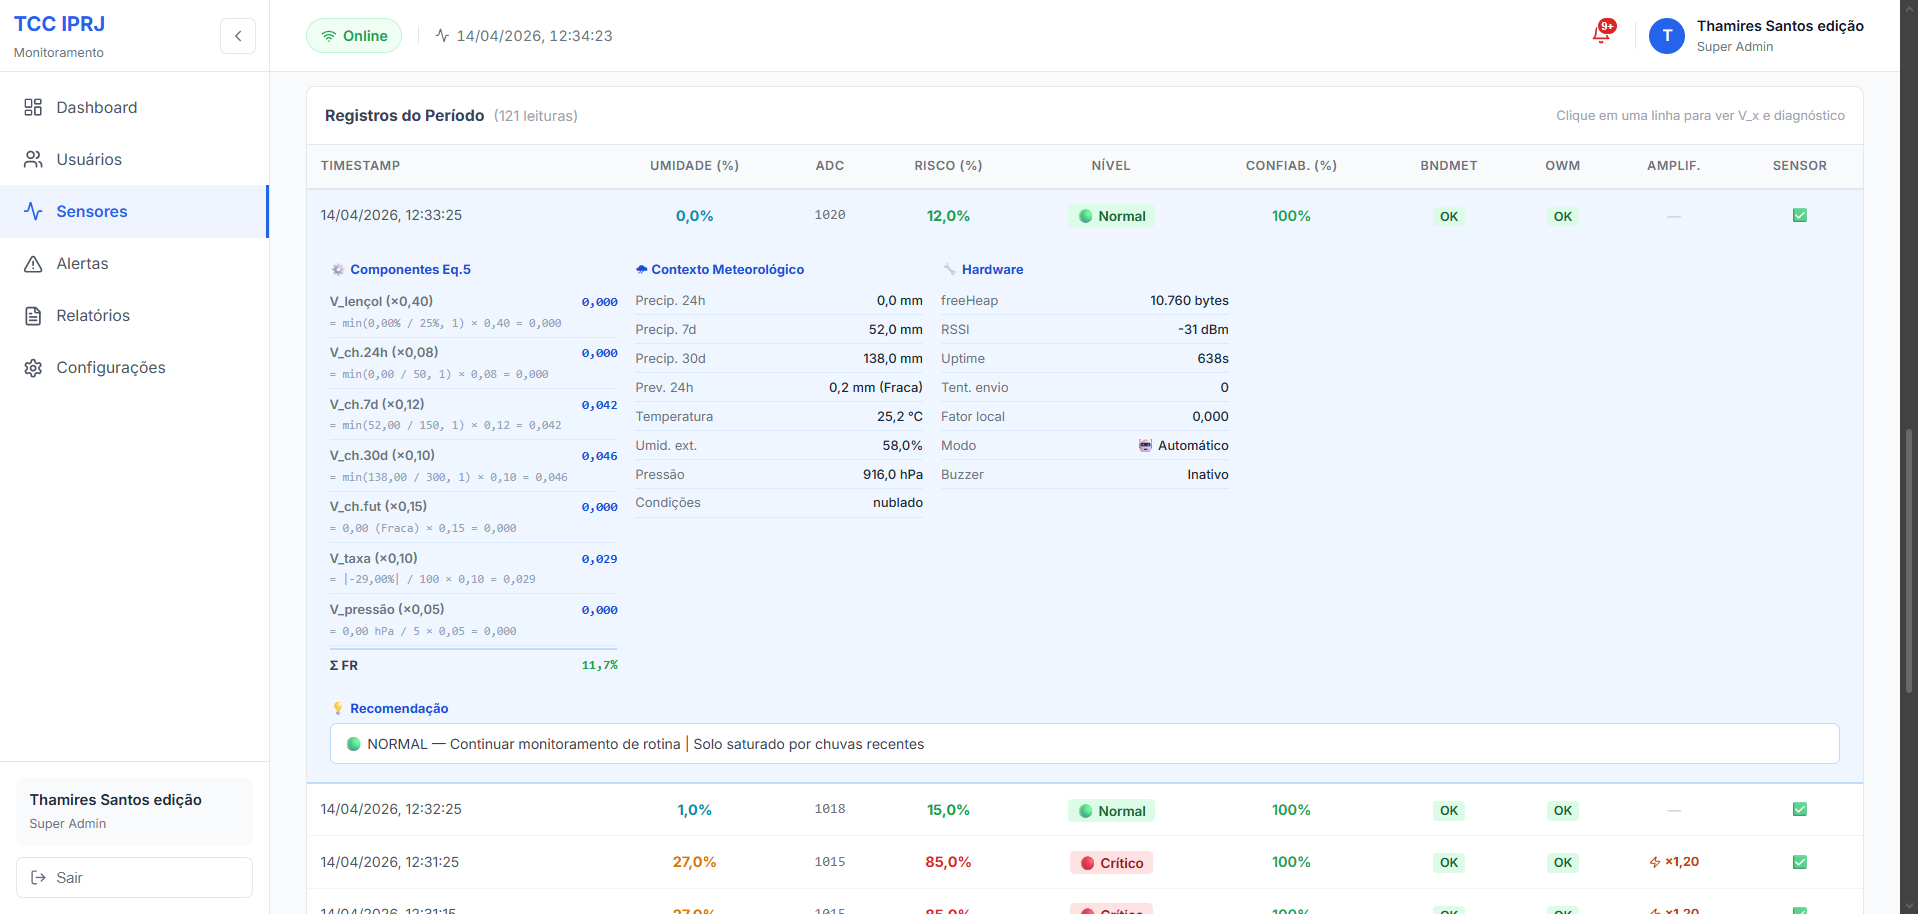
\includegraphics[width=0.95\textwidth]{figures/cap5_sensores_expandido_pt1.png}
    \caption{Linha expandida na tela de Sensores (parte~1): Nível Normal.}
    \label{fig:sensores_expandido_pt1}
    \fonte{Elaborado pela autora.}
\end{figure}

\begin{figure}[htbp]
    \centering
    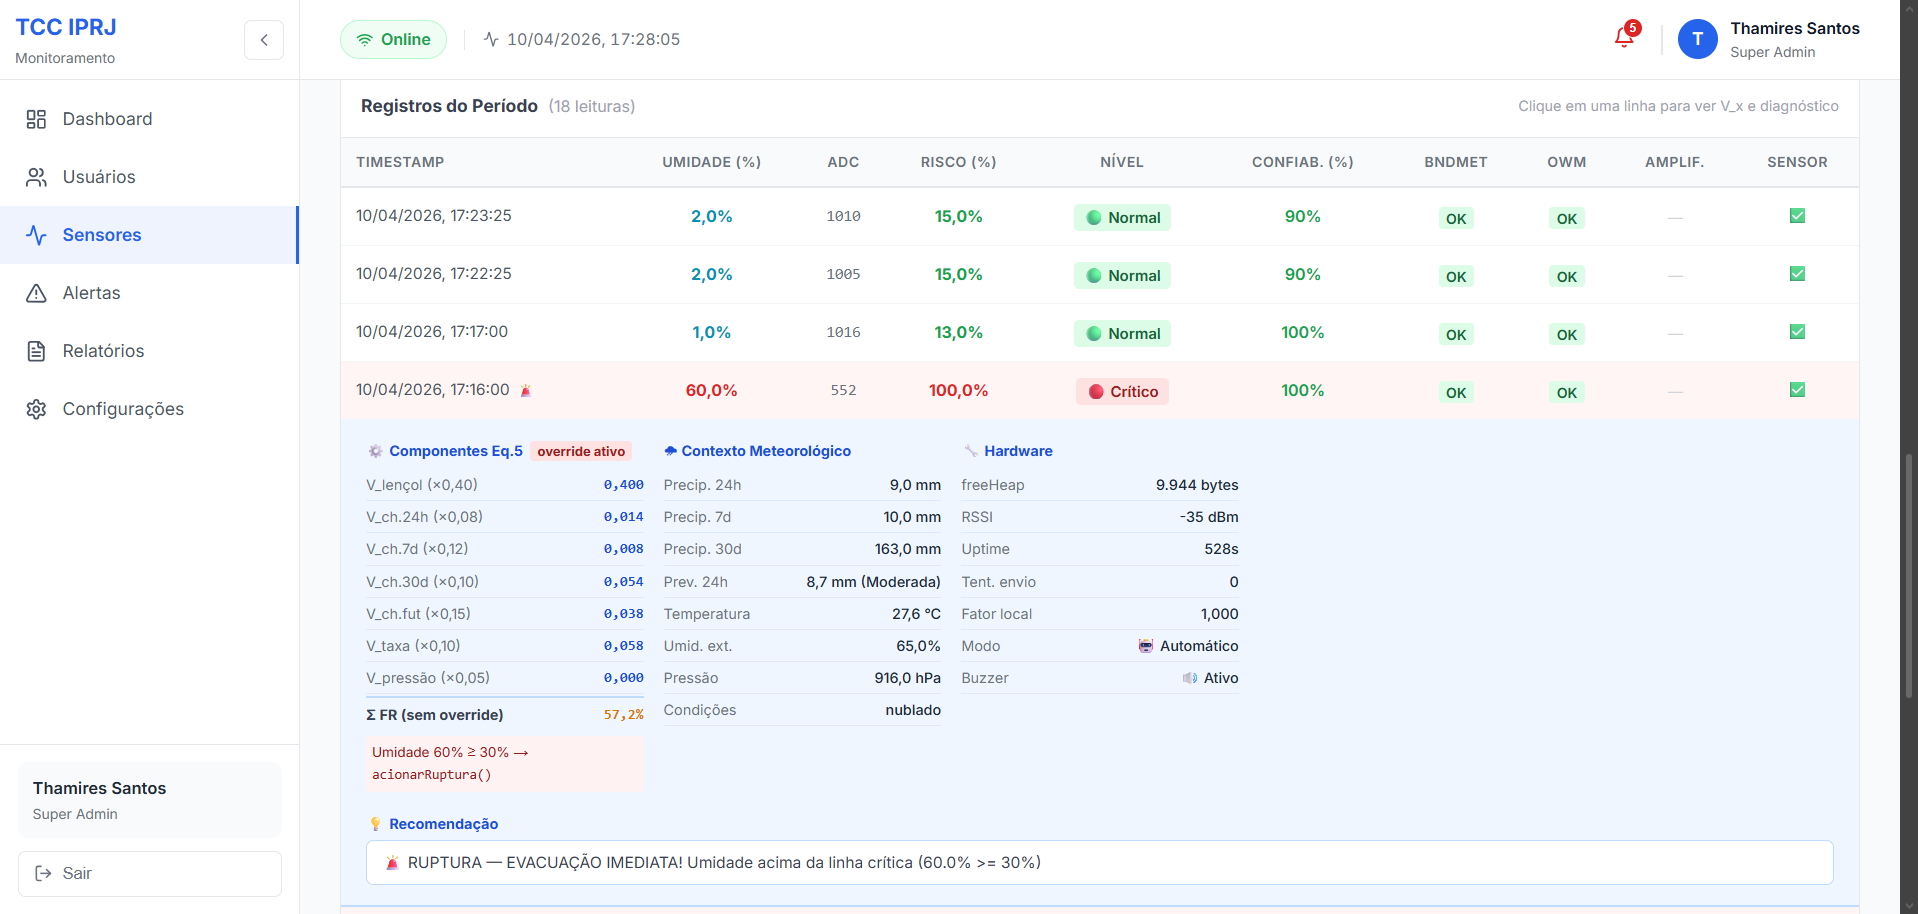
\includegraphics[width=0.95\textwidth]{figures/cap5_sensores_expandido_pt2.png}
    \caption{Linha expandida na tela de Sensores (parte~2): Nível Crítico (Ruptura).}
    \label{fig:sensores_expandido_pt2}
    \fonte{Elaborado pela autora.}
\end{figure}

\begin{figure}[htbp]
    \centering
    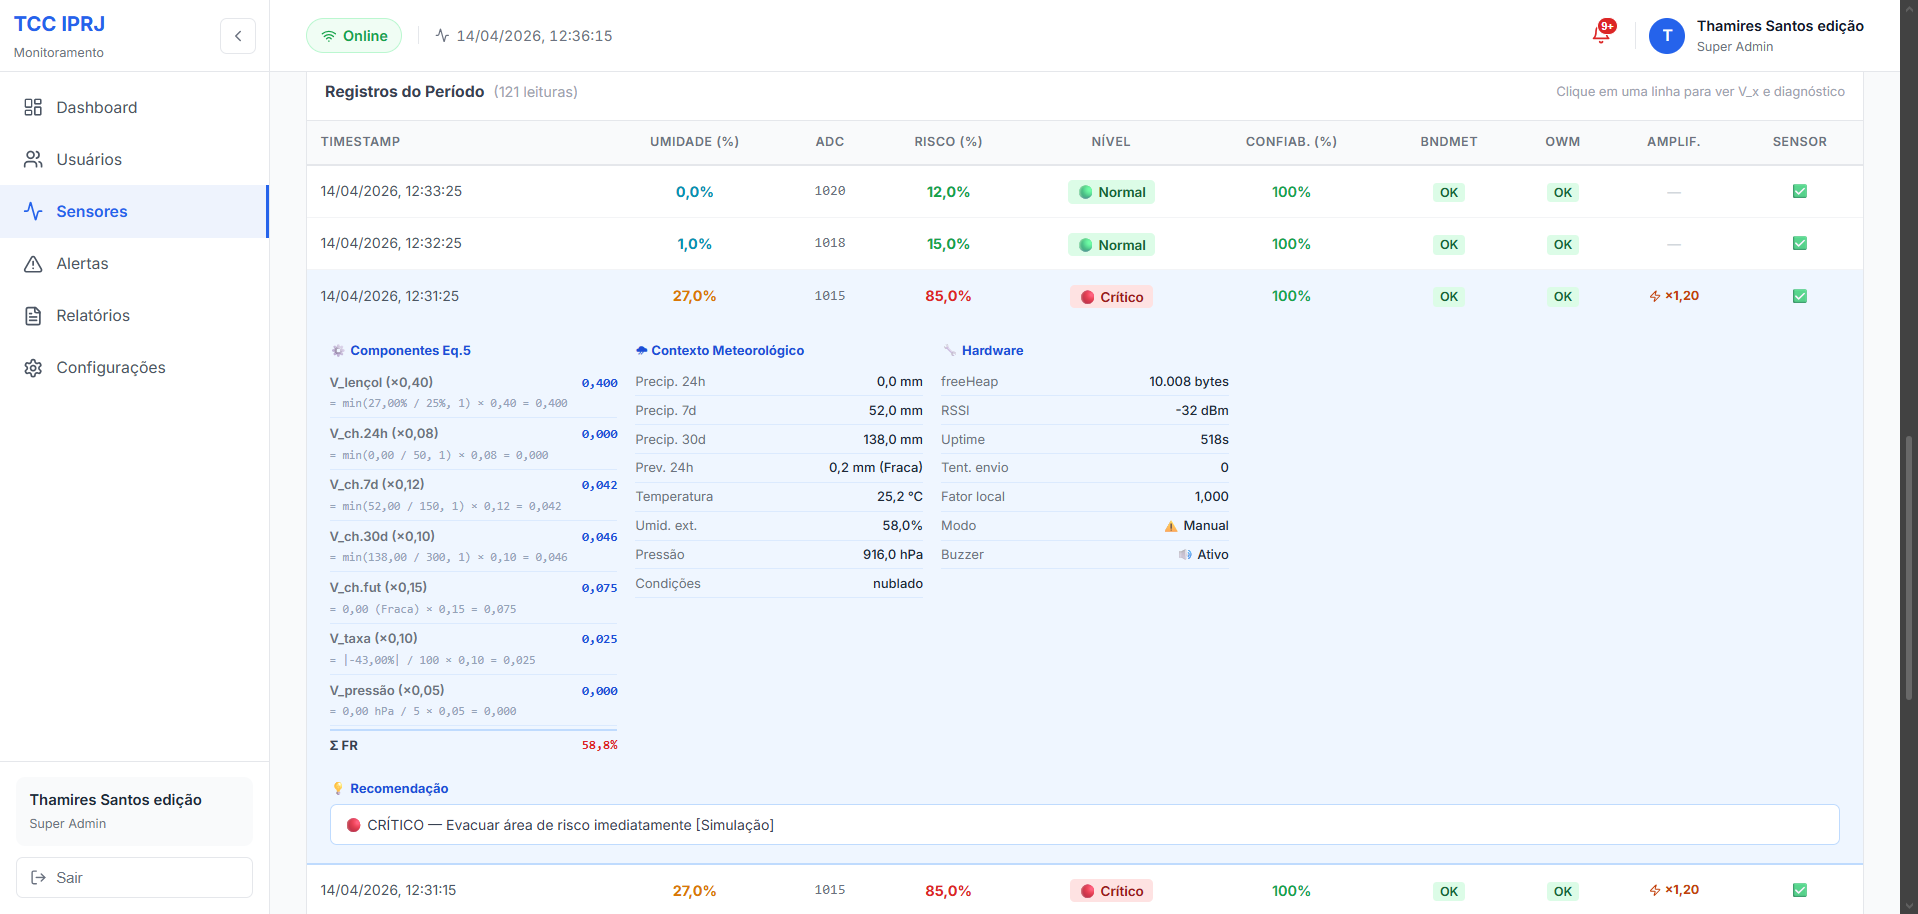
\includegraphics[width=0.95\textwidth]{figures/cap5_sensores_expandido_pt3.png}
    \caption{Linha expandida na tela de Sensores (parte~3): Nível Crítico.}
    \label{fig:sensores_expandido_pt3}
    \fonte{Elaborado pela autora.}
\end{figure}

\begin{figure}[htbp]
    \centering
    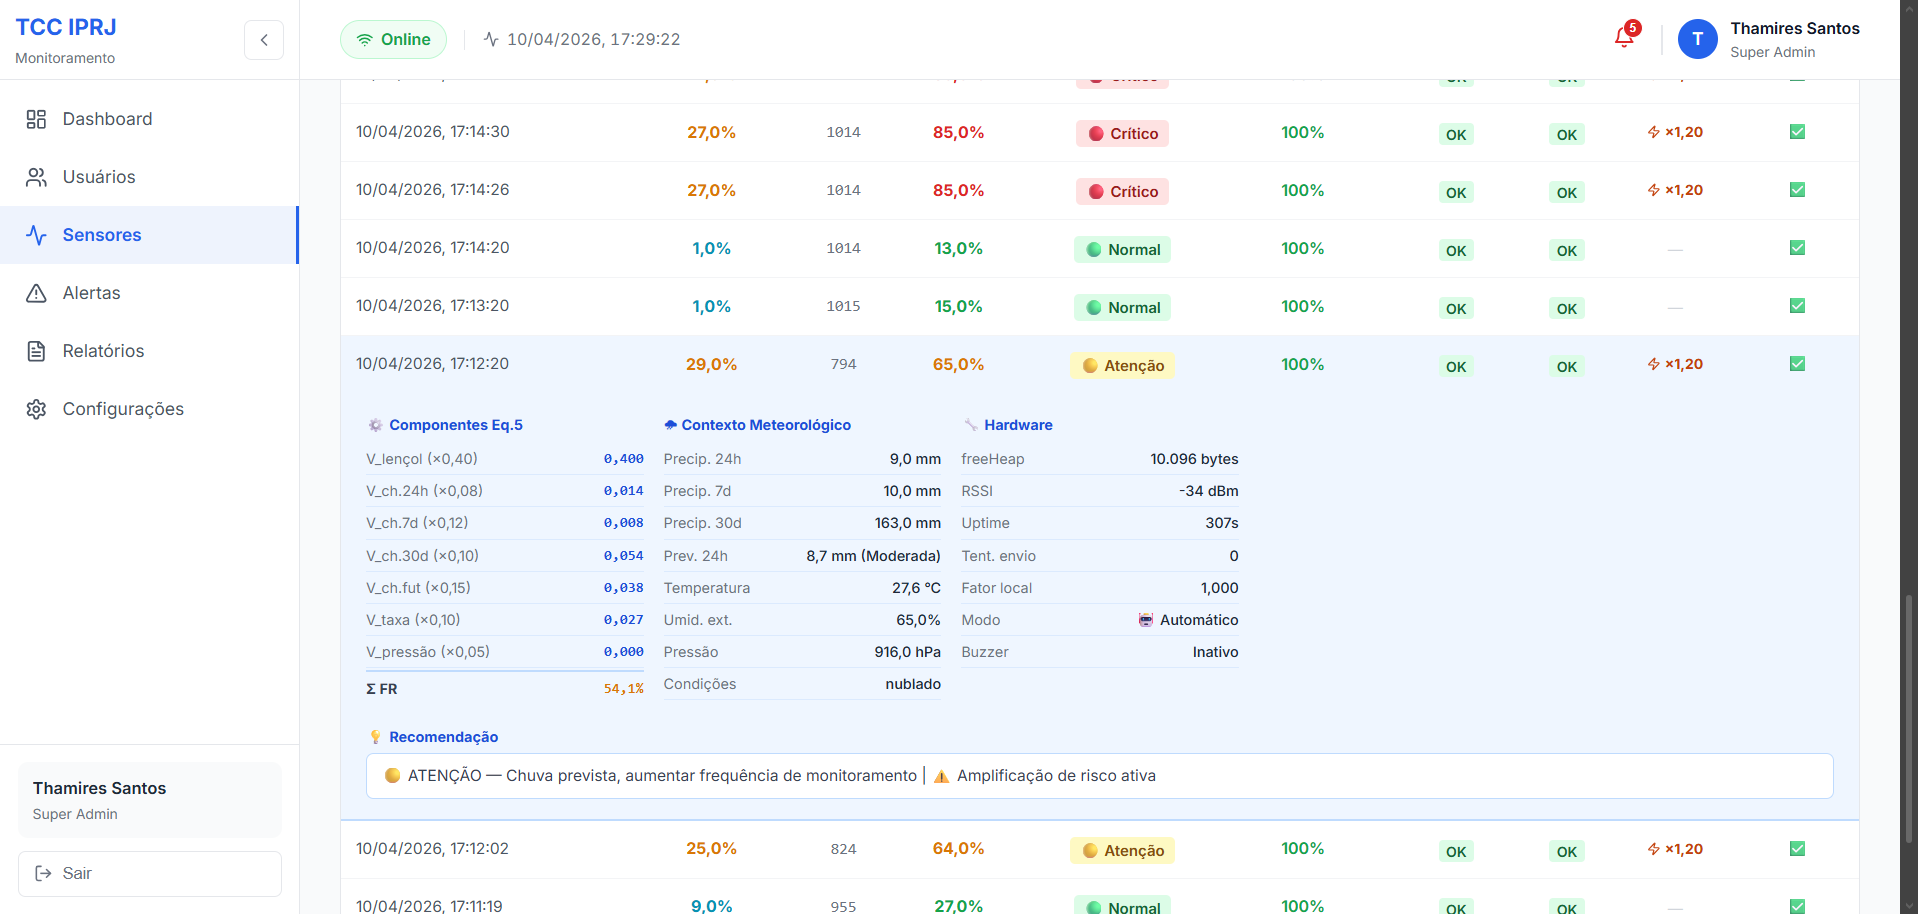
\includegraphics[width=0.95\textwidth]{figures/cap5_sensores_expandido_pt4.png}
    \caption{Linha expandida na tela de Sensores (parte~4): Nível Atenção.}
    \label{fig:sensores_expandido_pt4}
    \fonte{Elaborado pela autora.}
\end{figure}

% -------------------------------------------------------------
\subsection{Exportação de Leituras em CSV}
\label{subsec:sensores-csv}
% -------------------------------------------------------------
Quando o período selecionado contém leituras, o botão
\textbf{"CSV"} é exibido habilitado na interface, conforme
ilustra a \autoref{fig:sensores_csv_habilitado}. Ao clicar, o
sistema gera um arquivo com BOM UTF-8 para compatibilidade com
o Microsoft Excel, contendo todas as leituras do período com
41 colunas, e ao concluir, o \textit{toast} ``CSV exportado!'' confirma o 
\textit{download} automaticamente no navegador, conforme ilustra a \autoref{fig:sensores_csv_toast}.
O nome do arquivo inclui a data do dia da exportação.
 
\begin{figure}[htbp]
    \centering
    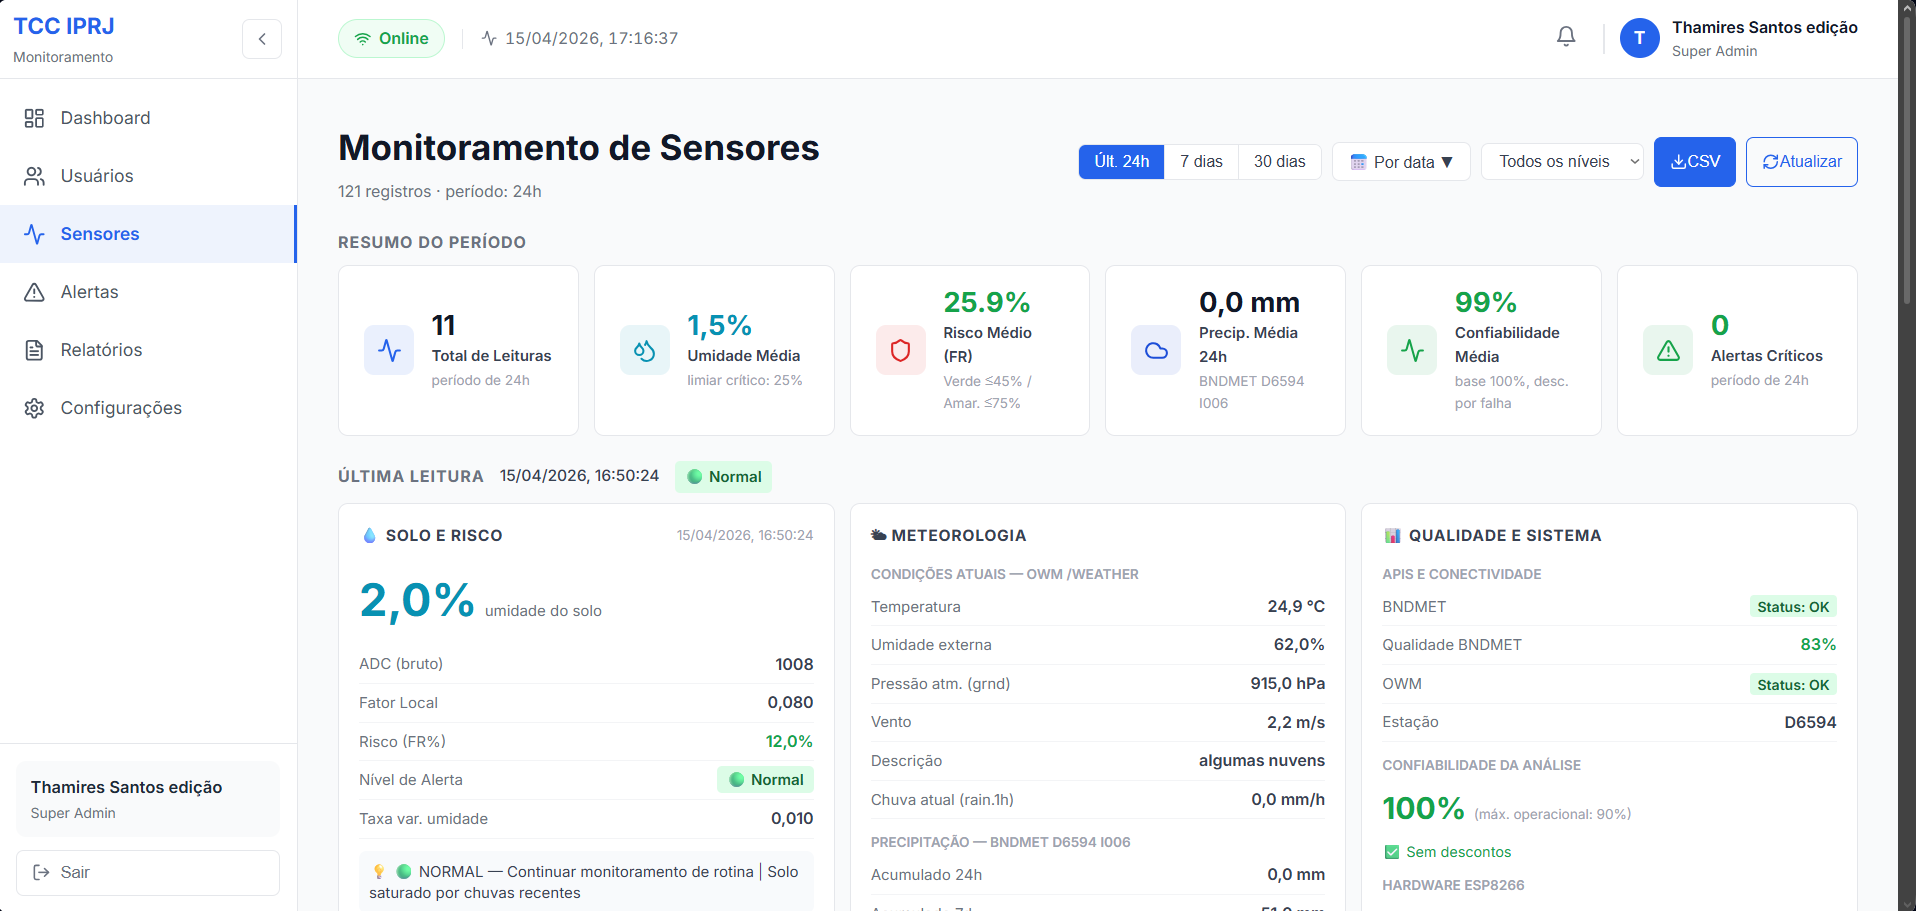
\includegraphics[width=0.85\textwidth]
        {figures/cap5_sensores_csv_habilitado.png}
    \caption{Tela de Sensores com botão \textbf{"CSV"} habilitado:
    período selecionado contém leituras disponíveis para
    exportação.}
    \label{fig:sensores_csv_habilitado}
    \fonte{Elaborado pela autora.}
\end{figure}
 
\begin{figure}[htbp]
    \centering
    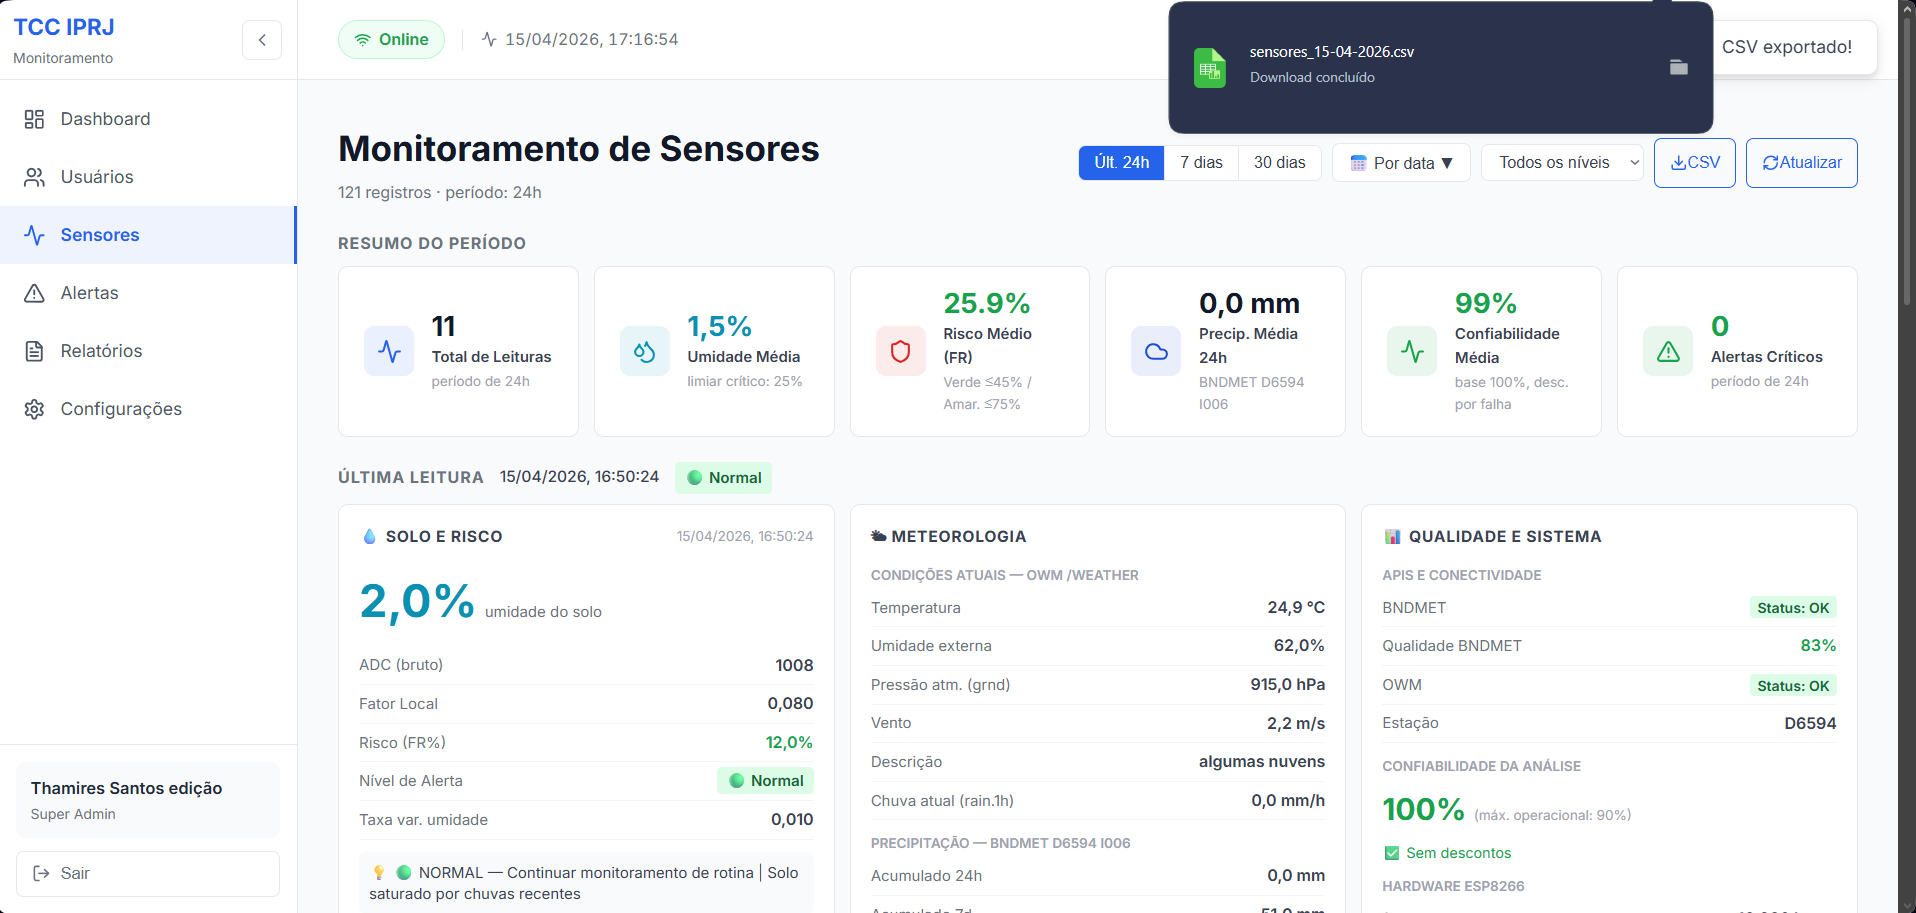
\includegraphics[width=0.85\textwidth]
        {figures/cap5_sensores_csv_toast.png}
    \caption{Tela de Sensores após exportação em CSV:
    \textit{download} iniciado e arquivo disponível no
    navegador.}
    \label{fig:sensores_csv_toast}
    \fonte{Elaborado pela autora.}
\end{figure}
 
As \autoref{fig:sensores_csv_pt1},
\autoref{fig:sensores_csv_pt2} e
\autoref{fig:sensores_csv_pt3} exibem o arquivo aberto no
Excel, com os cabeçalhos das colunas identificados.

\begin{figure}[htbp]
    \centering
    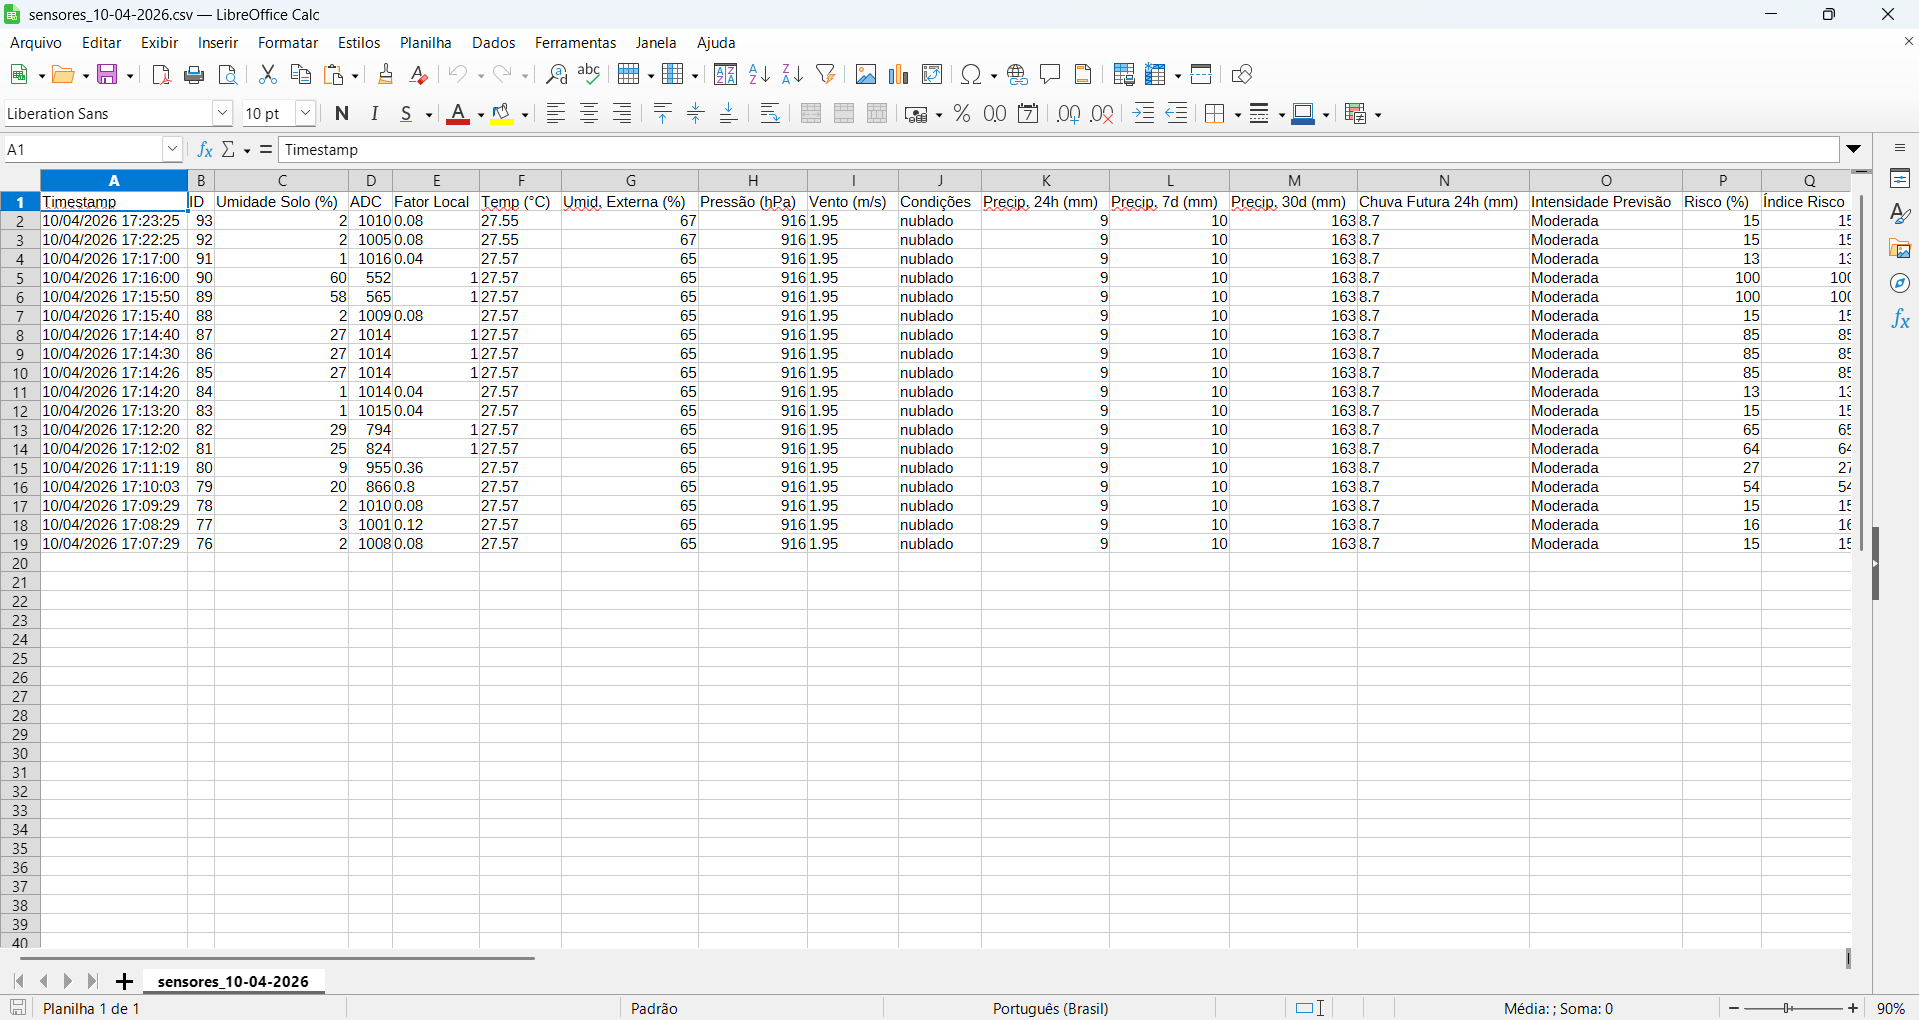
\includegraphics[width=0.95\textwidth]{figures/cap5_sensores_csv_pt1.png}
    \caption{Arquivo CSV exportado pela tela de Sensores aberto no
    Microsoft Excel (parte~1): cabeçalhos das primeiras colunas com dados
    de identificação e leitura do sensor.}
    \label{fig:sensores_csv_pt1}
    \fonte{Elaborado pela autora.}
\end{figure}

\begin{figure}[htbp]
    \centering
    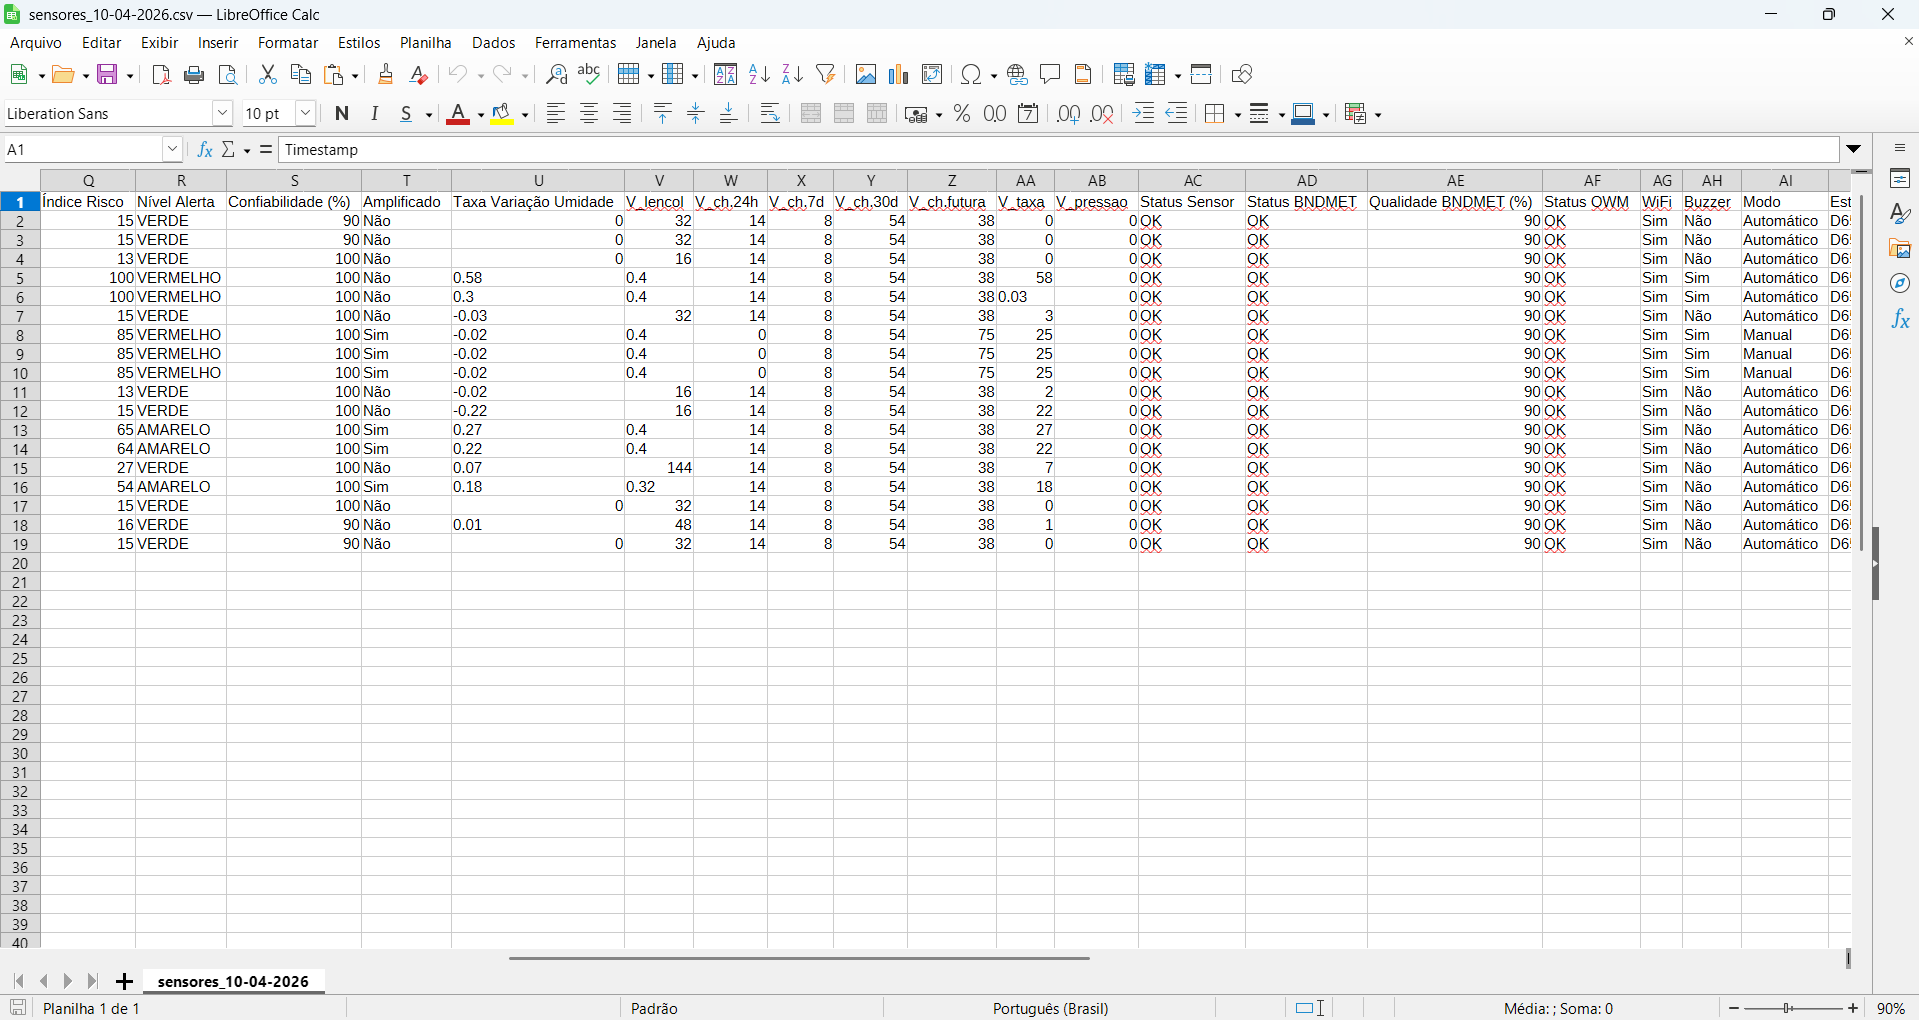
\includegraphics[width=0.95\textwidth]{figures/cap5_sensores_csv_pt2.png}
    \caption{Arquivo CSV exportado pela tela de Sensores aberto no
    Microsoft Excel (parte~2): colunas dos componentes individuais do
    modelo de risco.}
    \label{fig:sensores_csv_pt2}
    \fonte{Elaborado pela autora.}
\end{figure}

\begin{figure}[htbp]
    \centering
    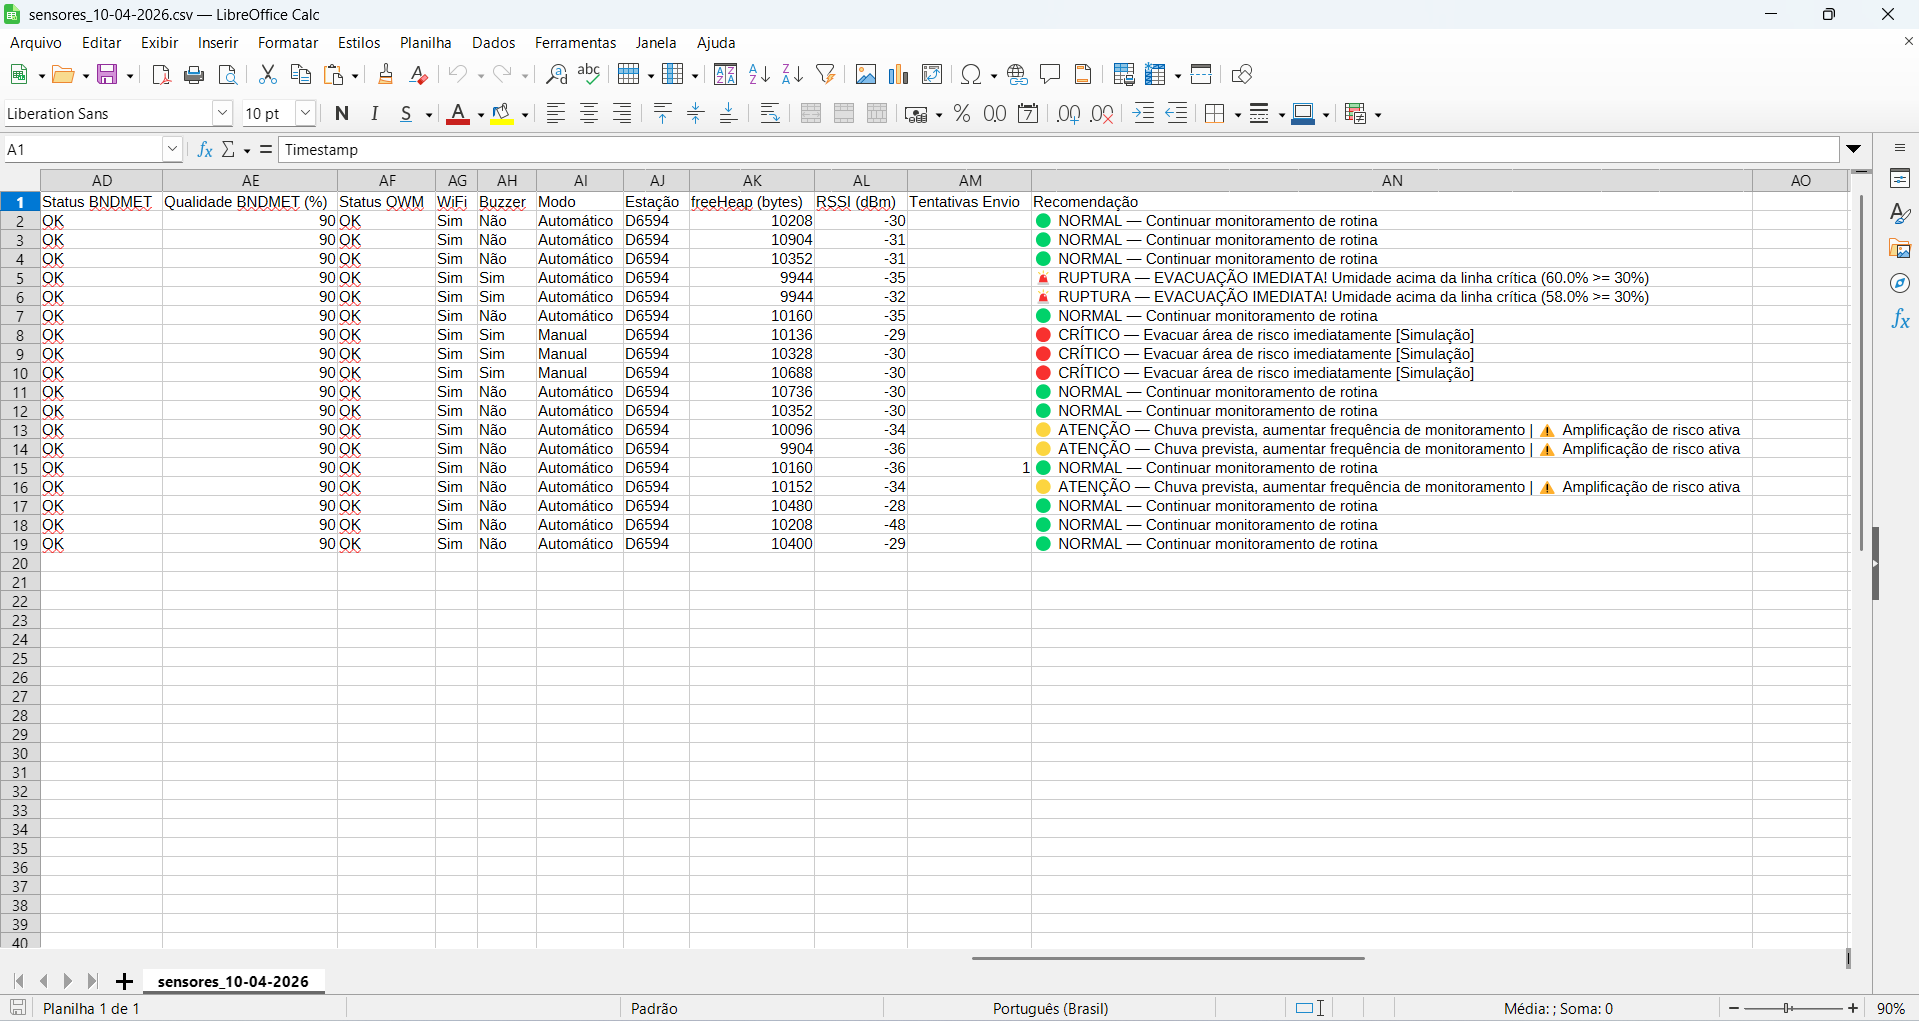
\includegraphics[width=0.95\textwidth]{figures/cap5_sensores_csv_pt3.png}
    \caption{Arquivo CSV exportado pela tela de Sensores aberto no
    Microsoft Excel (parte~3): colunas de dados meteorológicos e
    diagnóstico de \textit{hardware}, totalizando 41 colunas.}
    \label{fig:sensores_csv_pt3}
    \fonte{Elaborado pela autora.}
\end{figure}

Quando o conjunto de dados filtrado está vazio, o botão de exportação é
exibido desabilitado, conforme ilustra a \autoref{fig:sensores_csv_desabilitado}.

\begin{figure}[htbp]
    \centering
    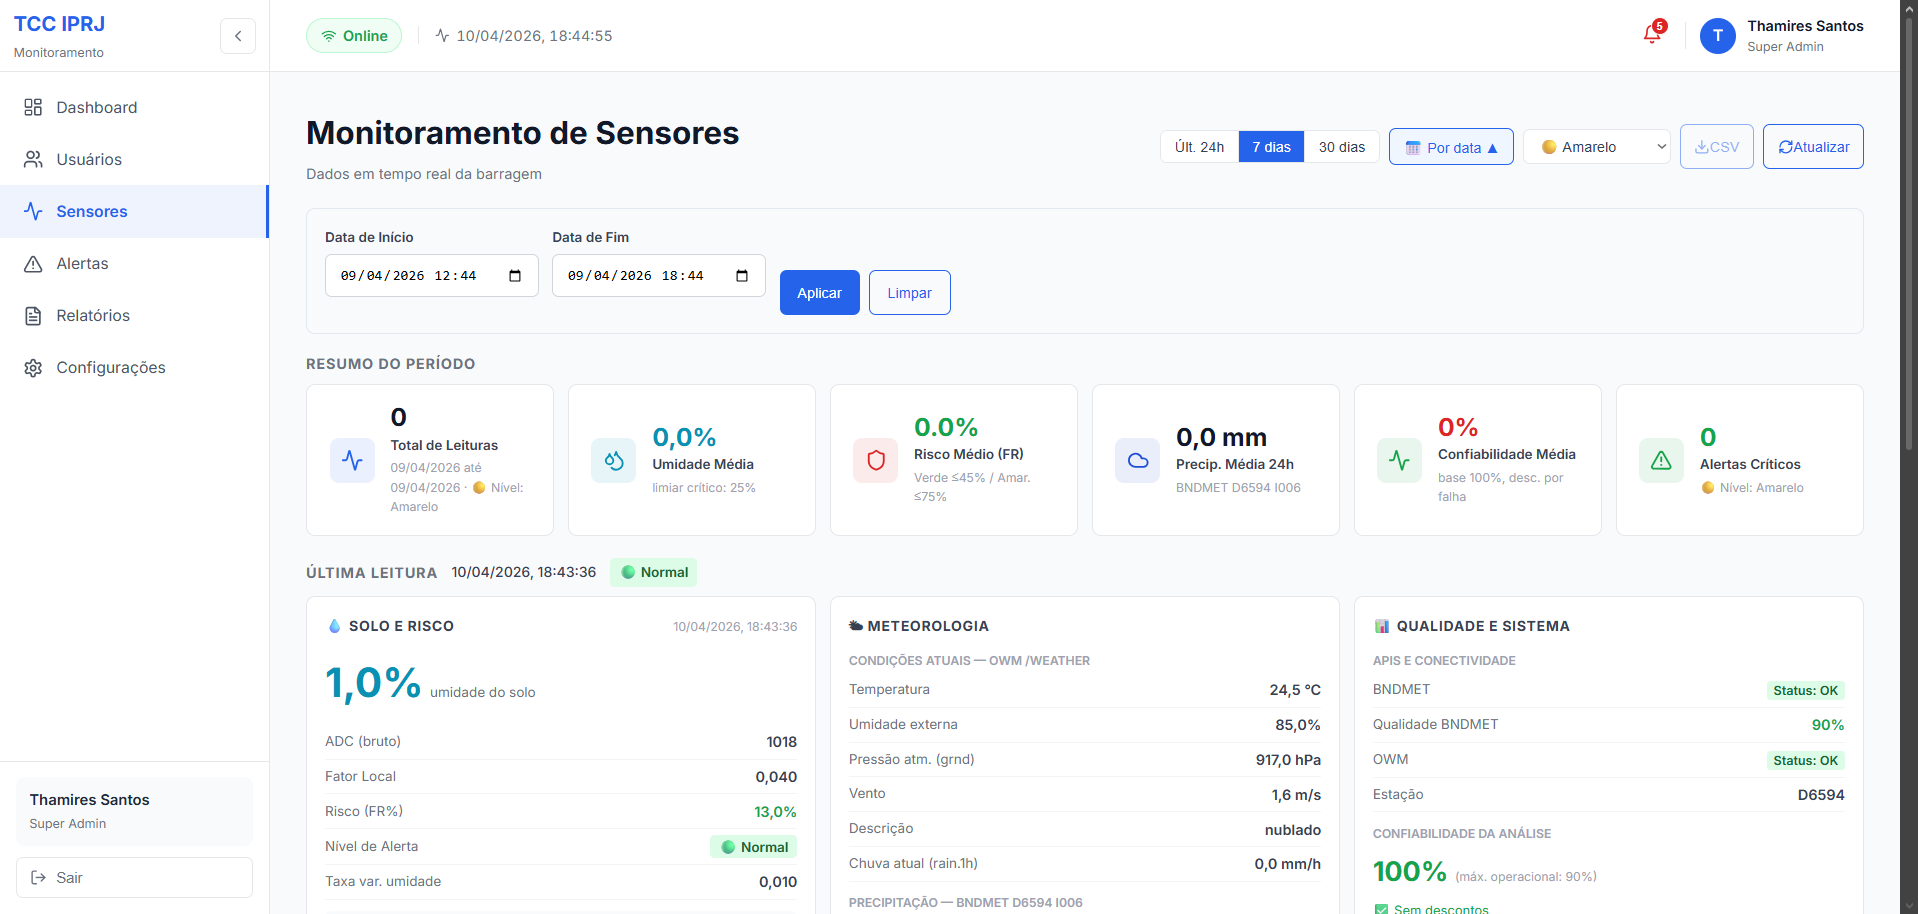
\includegraphics[width=0.95\textwidth]{figures/cap5_sensores_csv_desabilitado.png}
    \caption{Tela de Sensores com botão ``CSV'' desabilitado: nenhum registro disponível no conjunto filtrado atualmente visível na tabela.}
    \label{fig:sensores_csv_desabilitado}
    \fonte{Elaborado pela autora.}
\end{figure}

% =============================================================
\section{Central de Alertas}
\label{sec:alertas}
% =============================================================

% -------------------------------------------------------------
\subsection{Listagem e Filtro de Alertas Críticos}
\label{subsec:alertas-listagem}
% -------------------------------------------------------------

A Central de Alertas reúne todos os ciclos de leitura classificados como
AMARELO, VERMELHO ou RUPTURA. A \autoref{fig:alertas_lista} mostra a tela
com os cinco KPIs de contagem por categoria no topo --- Total, Crítico,
Atenção, Ruptura e Alertas enviados (30 dias) --- seguidos da lista
de alertas ordenada do mais recente para o mais antigo, com paginação
a 10 registros por página. Cada card exibe, em seu estado fechado, o \textit{timestamp},
o nível de alerta representado por um \textit{badge} colorido,
o índice de risco integrado e o botão \textbf{"Notificar"}.

\begin{figure}[htbp]
    \centering
    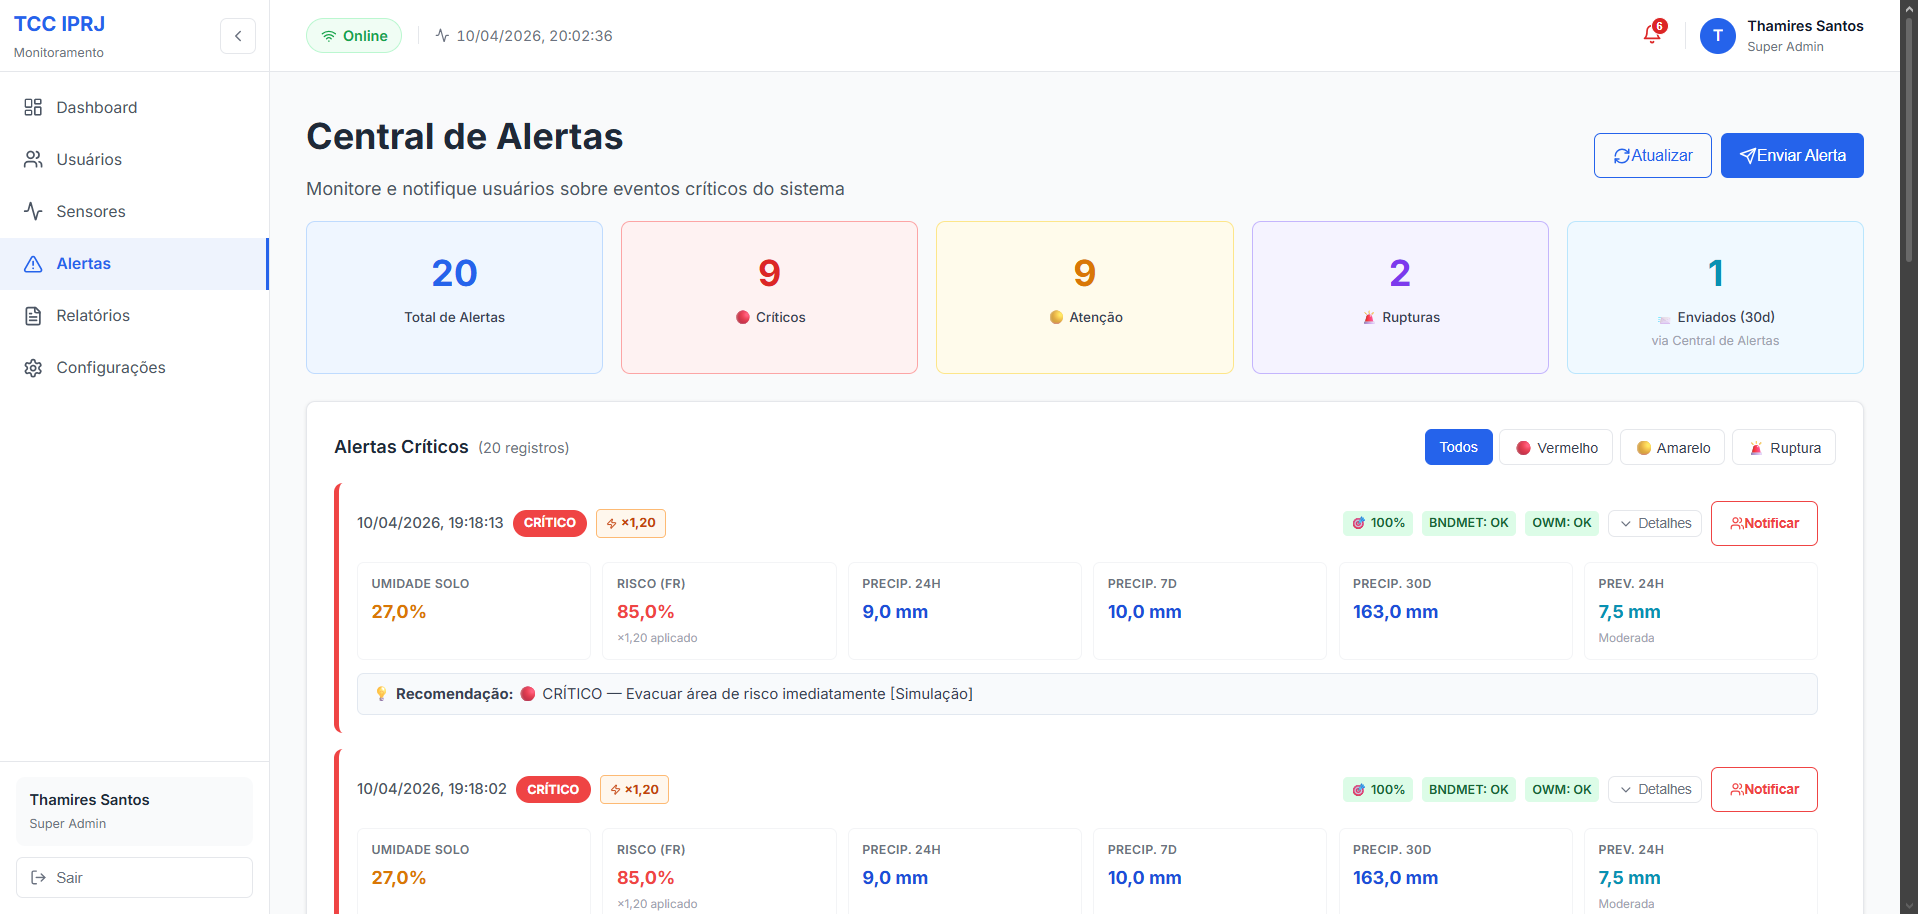
\includegraphics[width=0.95\textwidth]{figures/cap5_alertas_lista.png}
    \caption{Central de Alertas: KPIs de contagem por categoria e lista paginada de registros com card em estado fechado.}
    \label{fig:alertas_lista}
    \fonte{Elaborado pela autora.}
\end{figure}

Quando nenhum alerta está registrado no sistema, a tela exibe o estado
vazio com a mensagem ``Nenhum alerta encontrado'', conforme ilustra a \autoref{fig:alertas_lista_vazia}.

\begin{figure}[htbp]
    \centering
    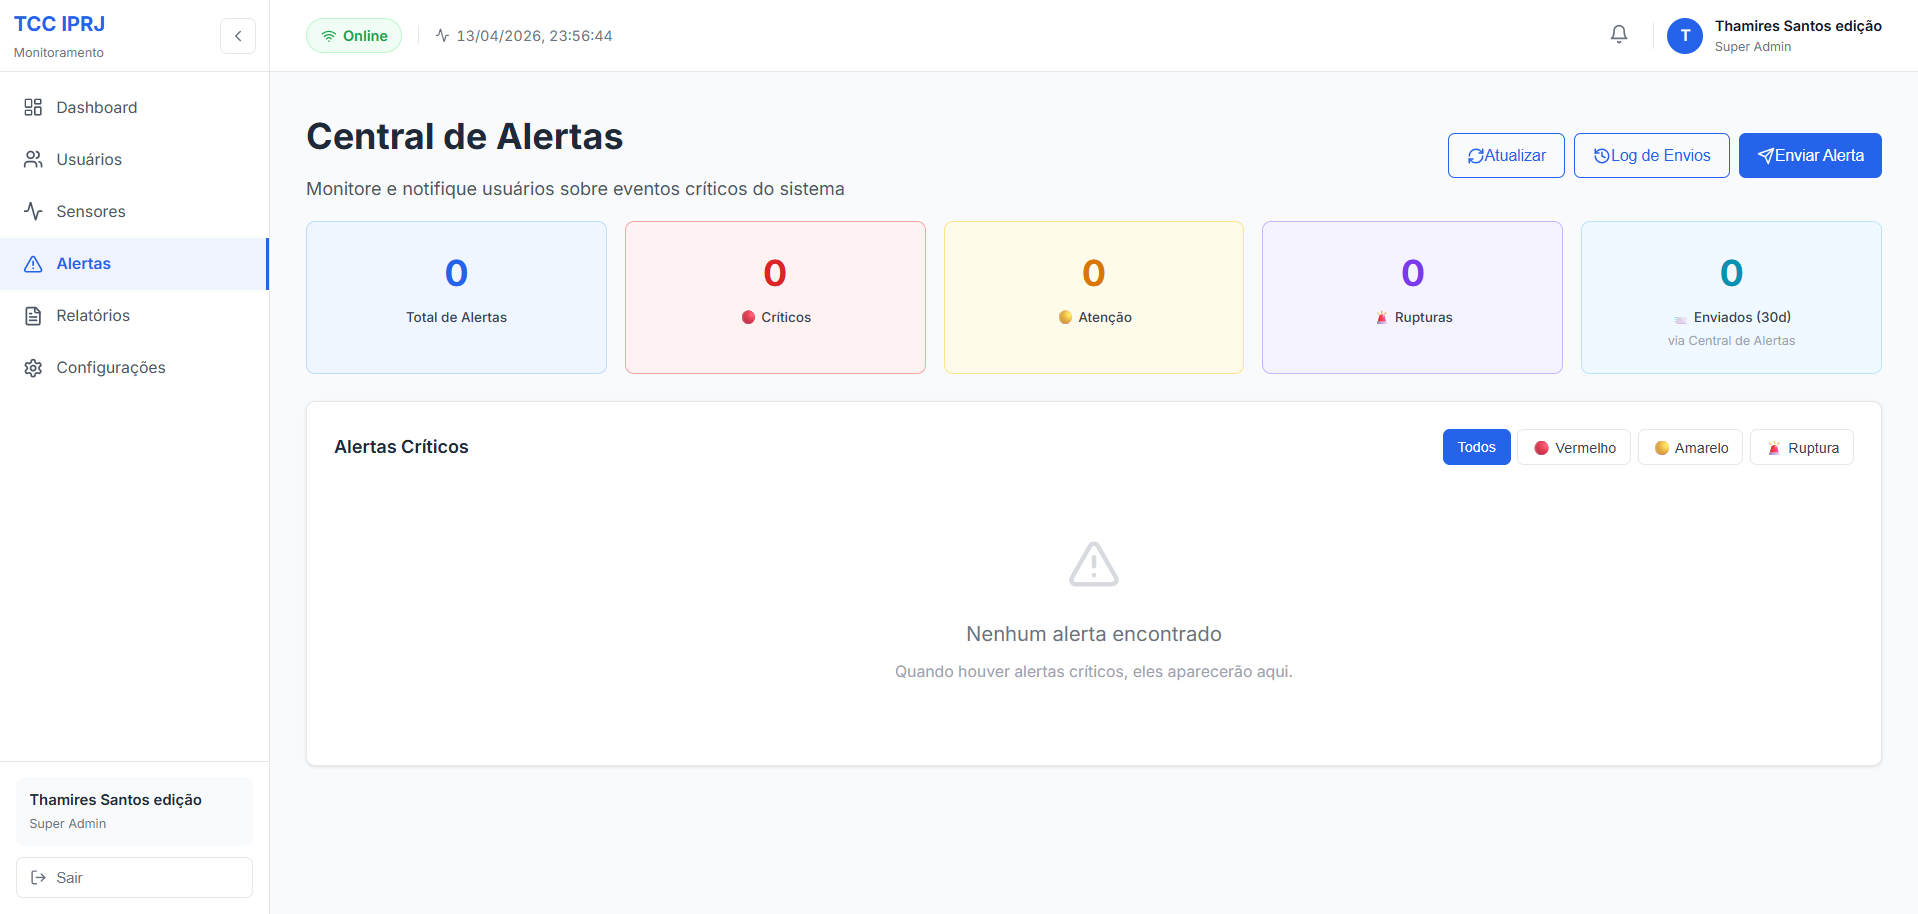
\includegraphics[width=0.95\textwidth]{figures/cap5_alertas_lista_vazia.png}
    \caption{Central de Alertas em estado vazio: mensagem ``Nenhum alerta encontrado'' exibida quando não há ciclos classificados como AMARELO, VERMELHO ou RUPTURA no sistema.}
    \label{fig:alertas_lista_vazia}
    \fonte{Elaborado pela autora.}
\end{figure}

Ao clicar em ``Notificar'' em um card específico, o formulário é aberto pré-preenchido com dados daquele ciclo de leitura, facilitando a composição da notificação pelo
administrador, como demonstram as \autoref{fig:alertas_form_preenchido_notificar_pt1} e \autoref{fig:alertas_form_preenchido_notificar_pt2}.

\begin{figure}[htbp]
    \centering
    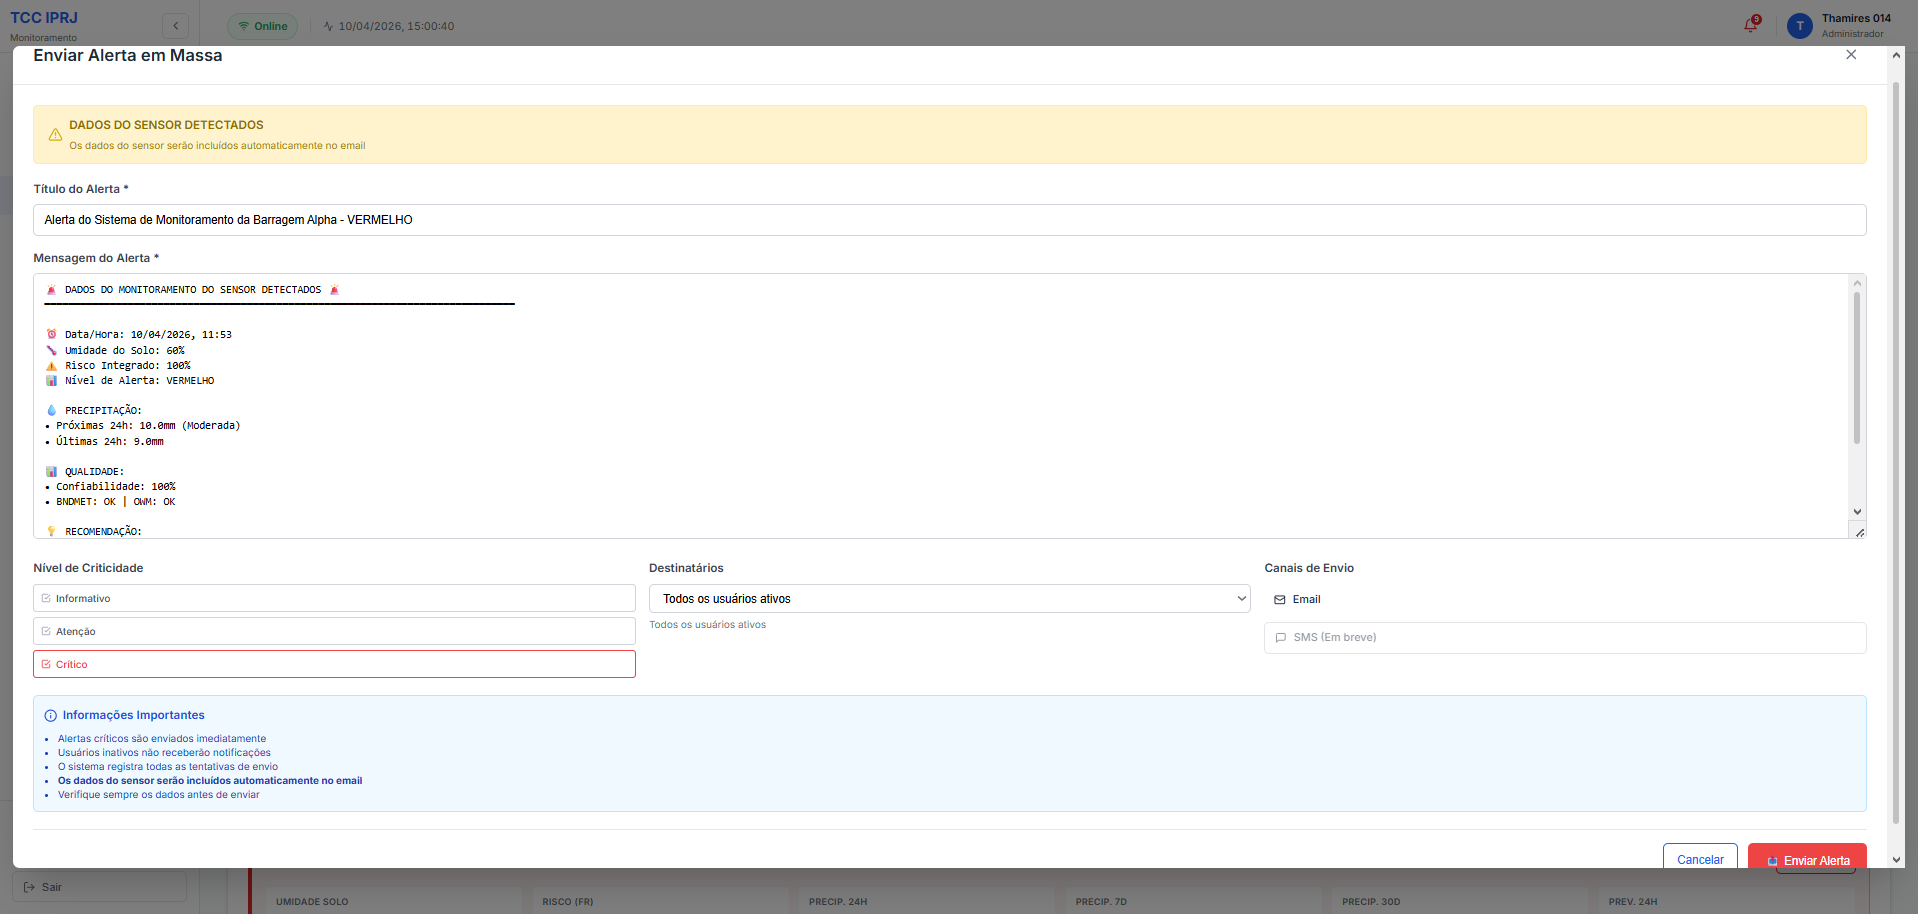
\includegraphics[width=0.80\textwidth]{figures/cap5_alertas_form_preenchido_notificar_pt1.png}
    \caption{Formulário de envio de alerta aberto a partir do botão ``Notificar'' de um card (parte~1): título pré-preenchido com os dados do ciclo de leitura selecionado.}
    \label{fig:alertas_form_preenchido_notificar_pt1}
    \fonte{Elaborado pela autora.}
\end{figure}

\begin{figure}[htbp]
    \centering
    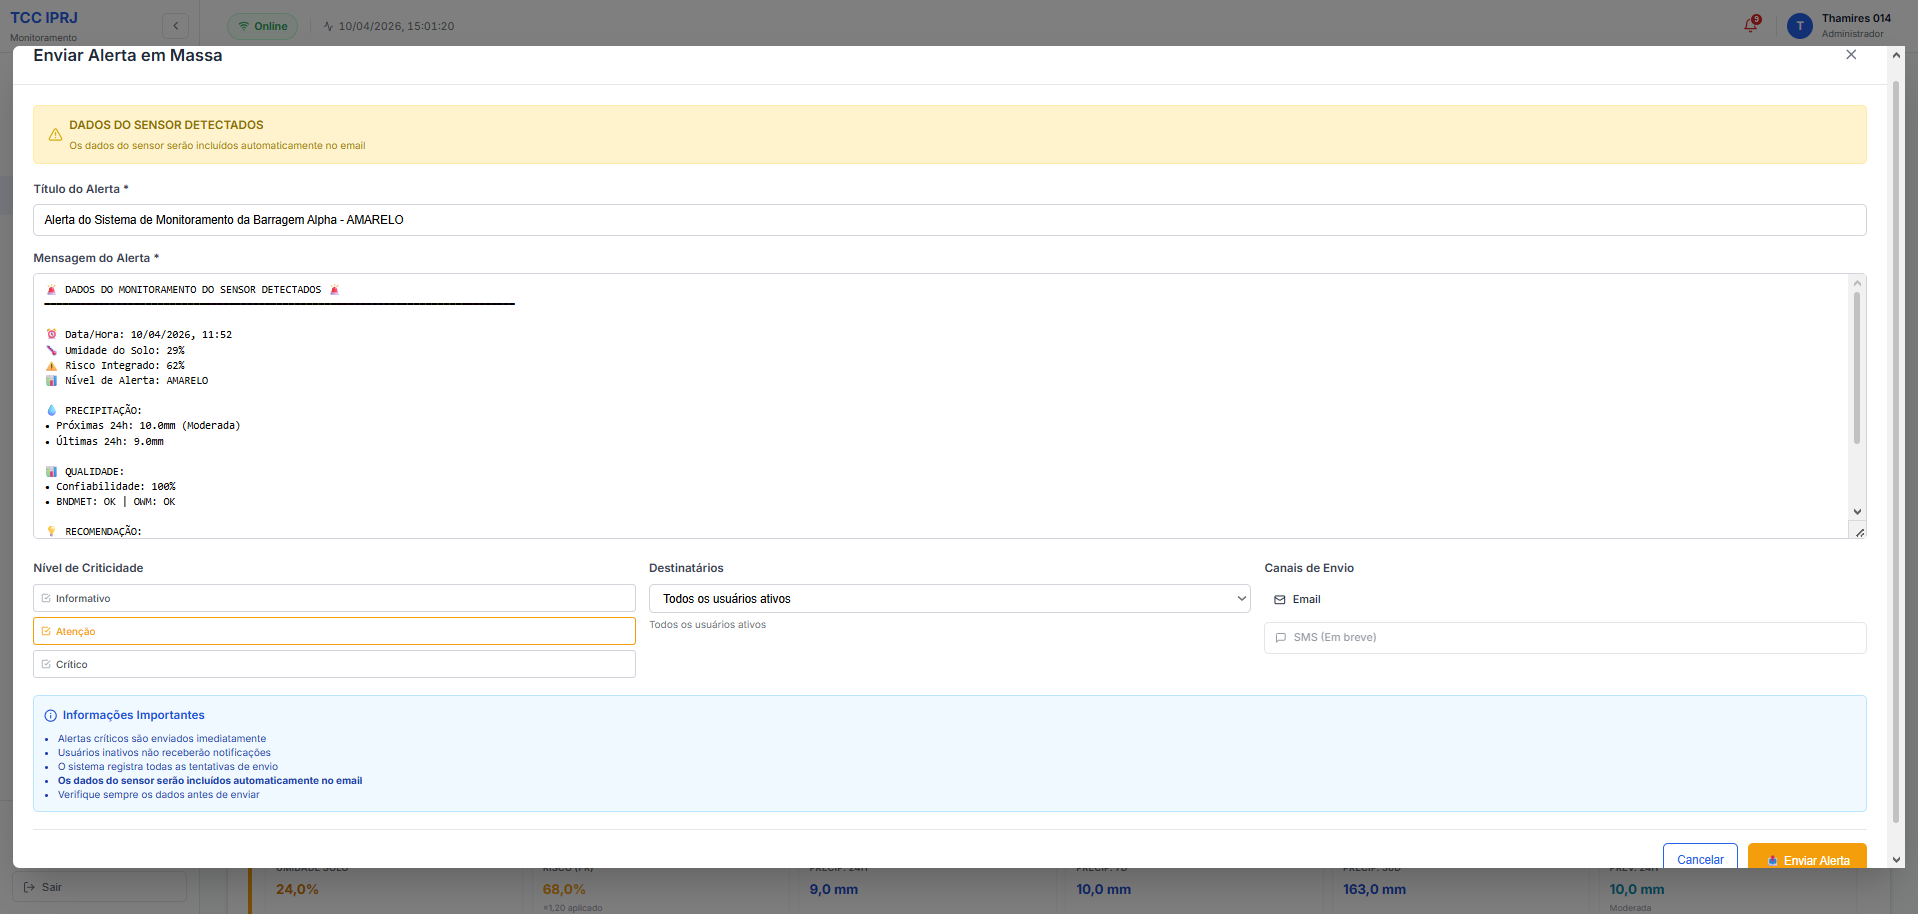
\includegraphics[width=0.80\textwidth]{figures/cap5_alertas_form_preenchido_notificar_pt2.png}
    \caption{Formulário de envio de alerta aberto a partir do botão ``Notificar'' de um card (parte~2): mensagem pré-preenchida com os dados do ciclo de leitura selecionado na Central de Alertas.}
    \label{fig:alertas_form_preenchido_notificar_pt2}
    \fonte{Elaborado pela autora.}
\end{figure}

Cada card de alerta é expansível ao clicar em ``Detalhes'' e, além dos quatro blocos de detalhe
presentes na tela de Sensores, exibe um quinto bloco exclusivo ---
``Cálculo de Confiabilidade'' --- que apresenta os descontos individuais
aplicados naquele ciclo, com desconto máximo possível, valor aplicado e
descrição da condição que motivou cada penalidade. A linha de rodapé do
bloco mostra o resultado final: 100\% menos o total de descontos
acumulados. Na situação especial de RUPTURA, o bloco exibe a mensagem
``100\% --- Estado Especial: RUPTURA'', informando que a confiabilidade
é fixada pelo hardware e não sofre descontos. Os níveis Vermelho, Amarelo e Ruptura são exibidos
conforme ilustram as \autoref{fig:alertas_expandido_pt1},
\autoref{fig:alertas_expandido_pt2} e
\autoref{fig:alertas_expandido_pt3}, respectivamente.

\begin{figure}[htbp]
    \centering
    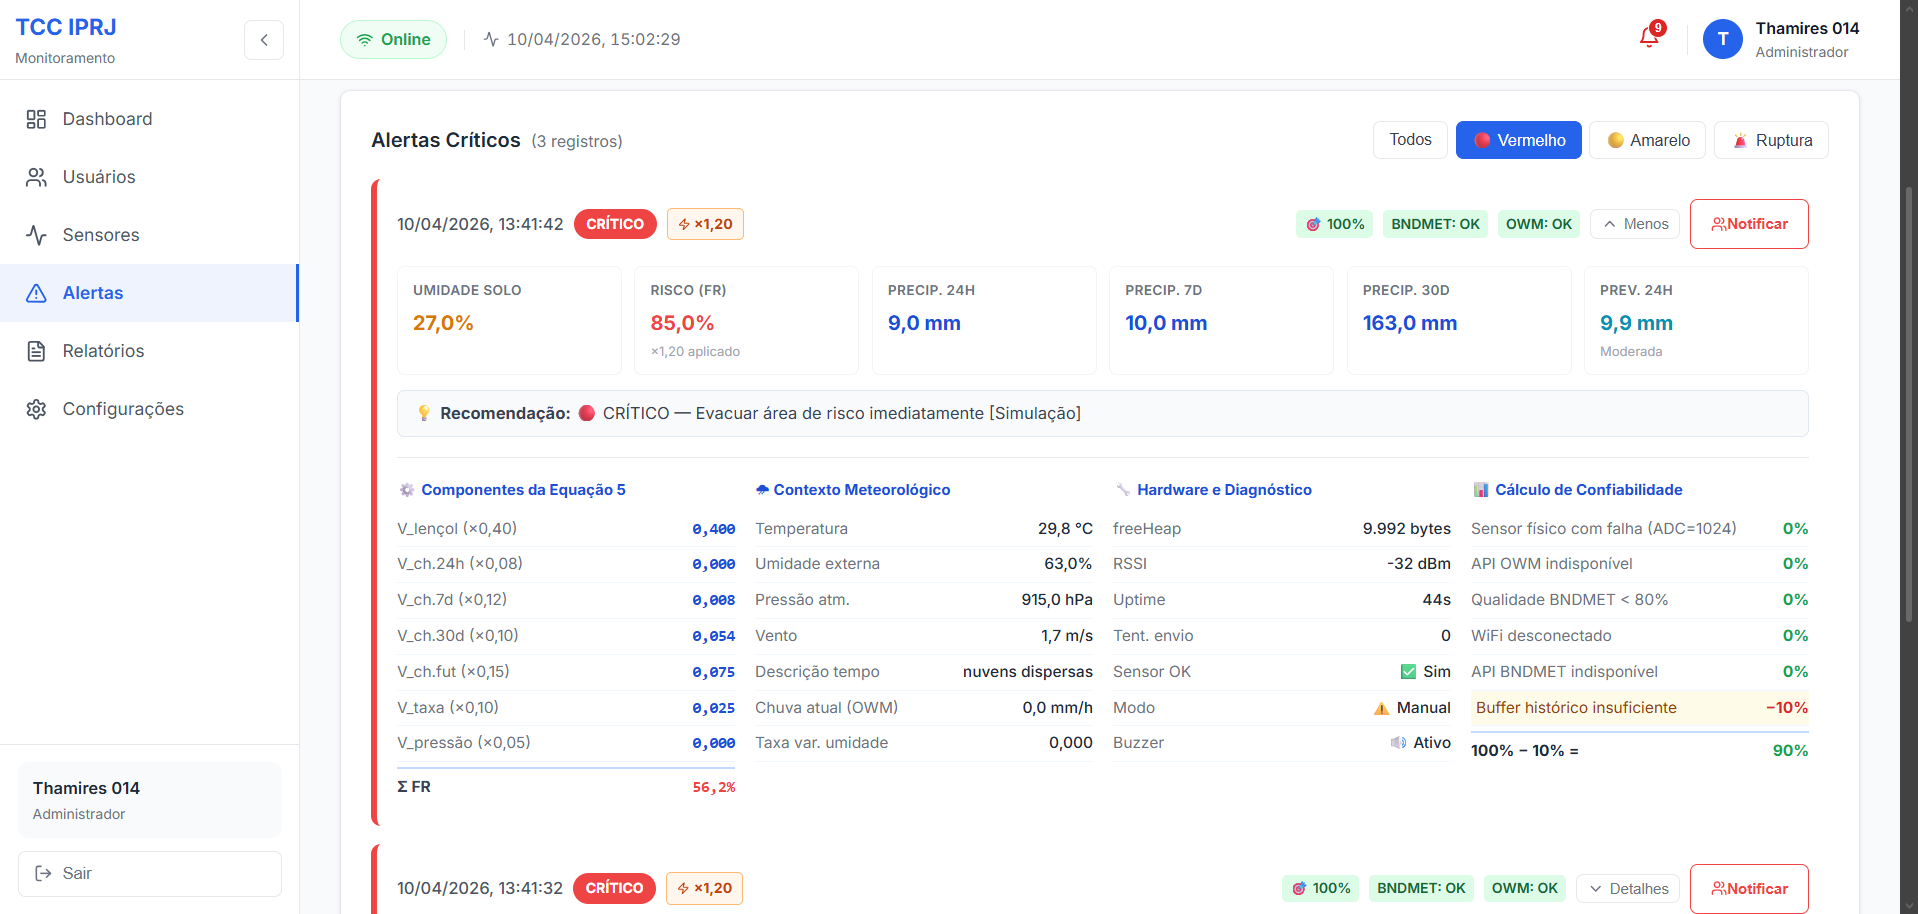
\includegraphics[width=0.95\textwidth]{figures/cap5_alertas_expandido_pt1.png}
    \caption{Card de alerta expandido na Central de Alertas (parte~1): nível Vermelho.}
    \label{fig:alertas_expandido_pt1}
    \fonte{Elaborado pela autora.}
\end{figure}

\begin{figure}[htbp]
    \centering
    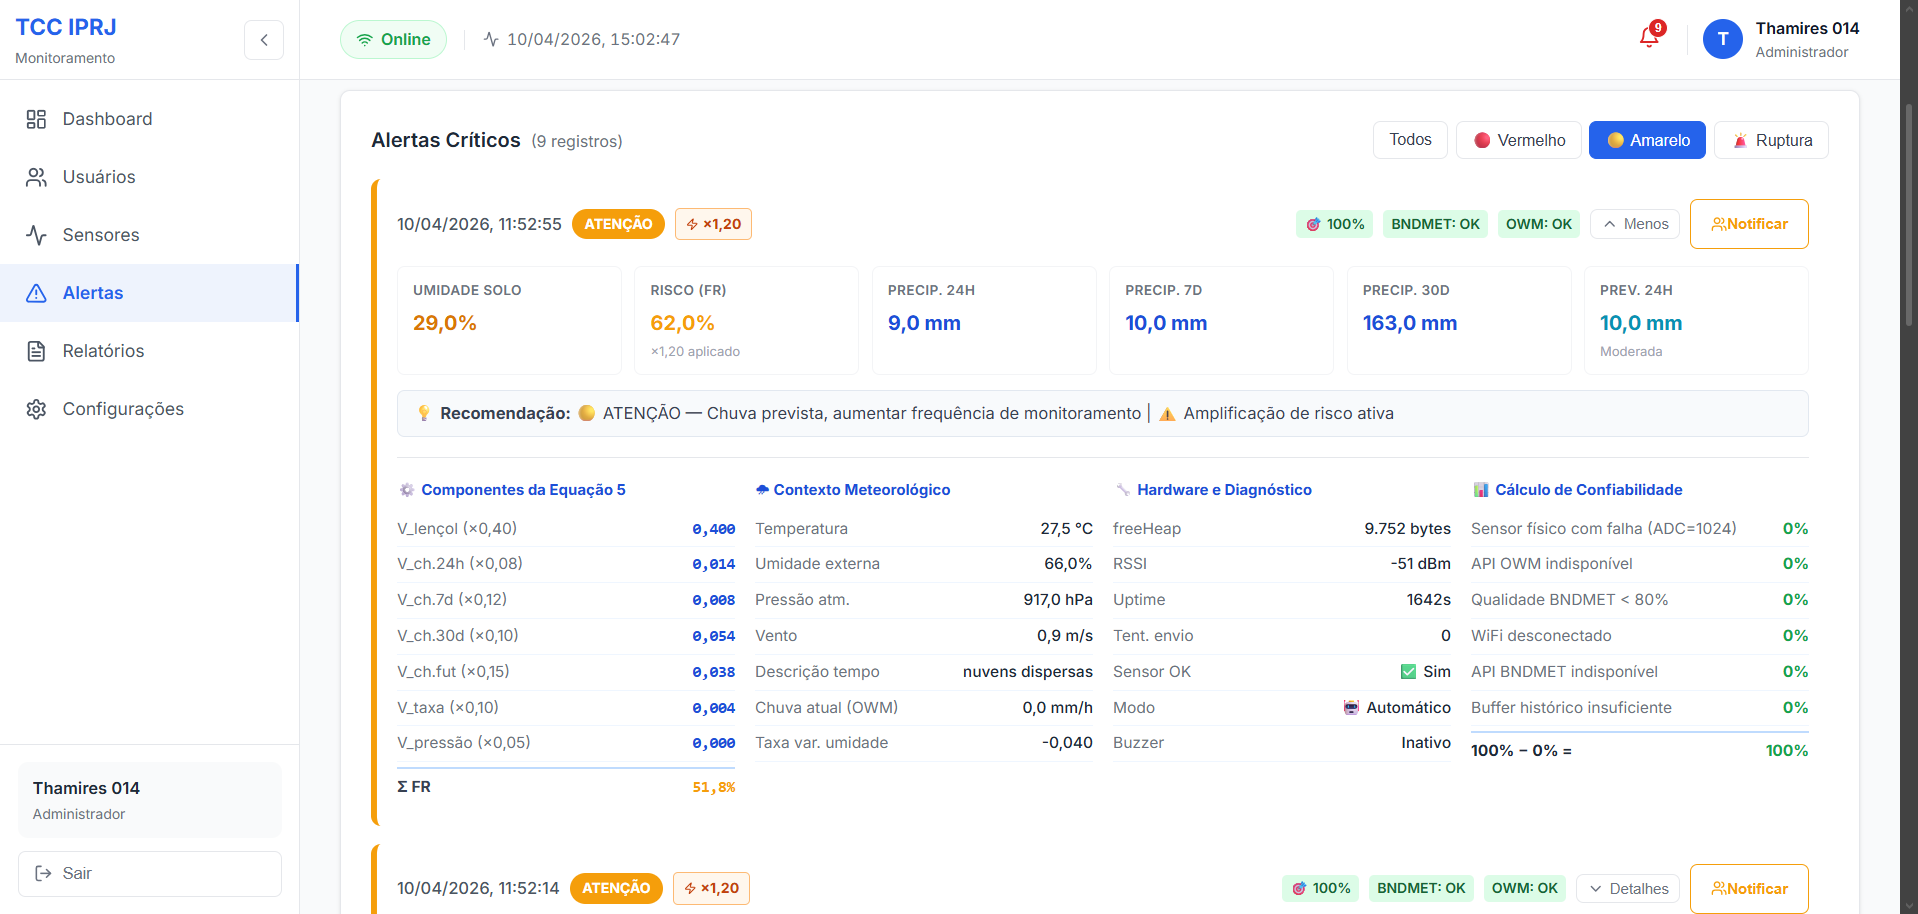
\includegraphics[width=0.95\textwidth]{figures/cap5_alertas_expandido_pt2.png}
    \caption{Card de alerta expandido na Central de Alertas (parte~2): nível Amarelo.}
    \label{fig:alertas_expandido_pt2}
    \fonte{Elaborado pela autora.}
\end{figure}

\begin{figure}[htbp]
    \centering
    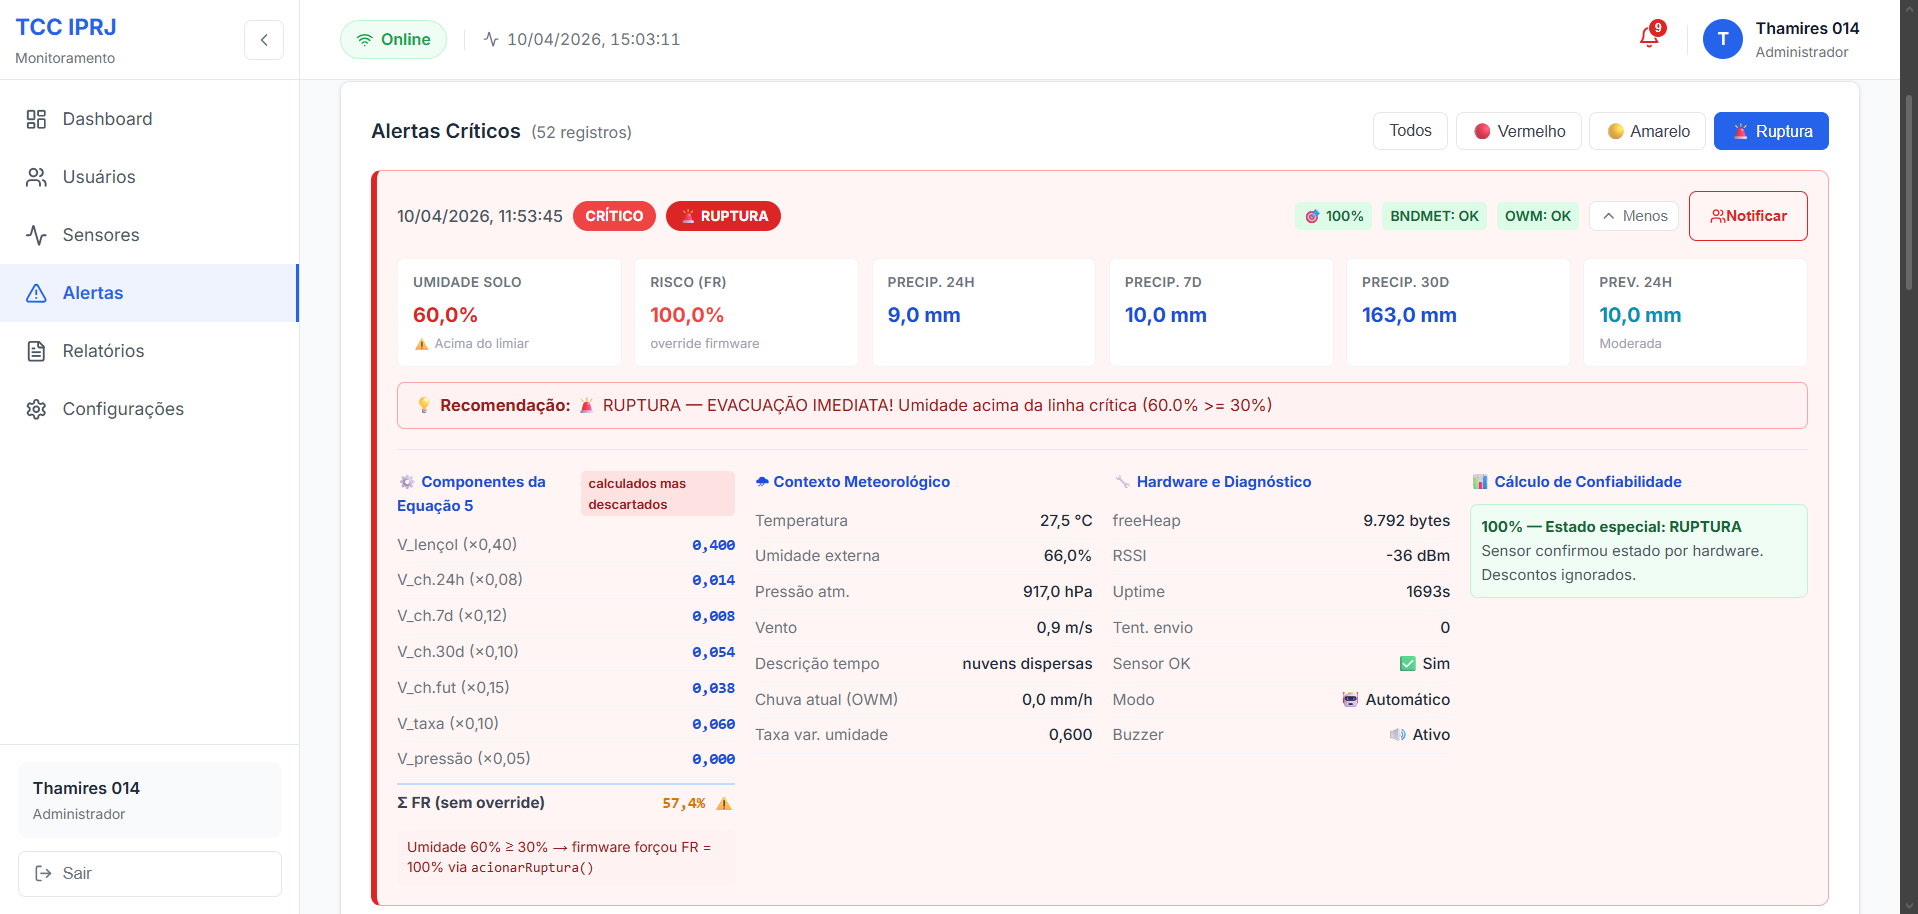
\includegraphics[width=0.95\textwidth]{figures/cap5_alertas_expandido_pt3.png}
    \caption{Card de alerta expandido na Central de Alertas (parte~3): nível Ruptura.}
    \label{fig:alertas_expandido_pt3}
    \fonte{Elaborado pela autora.}
\end{figure}

% -------------------------------------------------------------
\subsection{Envio de Alerta Manual em Massa}
\label{subsec:alertas-envio}
% -------------------------------------------------------------

O envio de alertas é sempre acionado manualmente pelo administrador.
Ao clicar em ``Enviar Alerta'' --- seja no cabeçalho da tela para um
alerta novo, seja no botão ``Notificar'' de um card específico ---,
o formulário \texttt{AlertForm} é aberto em um modal, como ilustra a
\autoref{fig:alertas_formulario}. O formulário apresenta os campos de
título (de 5 a 200 caracteres), mensagem (de 10 a 1.000 caracteres),
nível de criticidade com prévia visual da cor, tipo de destinatário
(todos os usuários ativos, apenas usuários básicos ou apenas administradores)
e canal de envio. Três \textit{templates} pré-definidos permitem
preencher título e mensagem com um clique; o administrador pode editar
os campos antes de confirmar.

\begin{figure}[htbp]
    \centering
    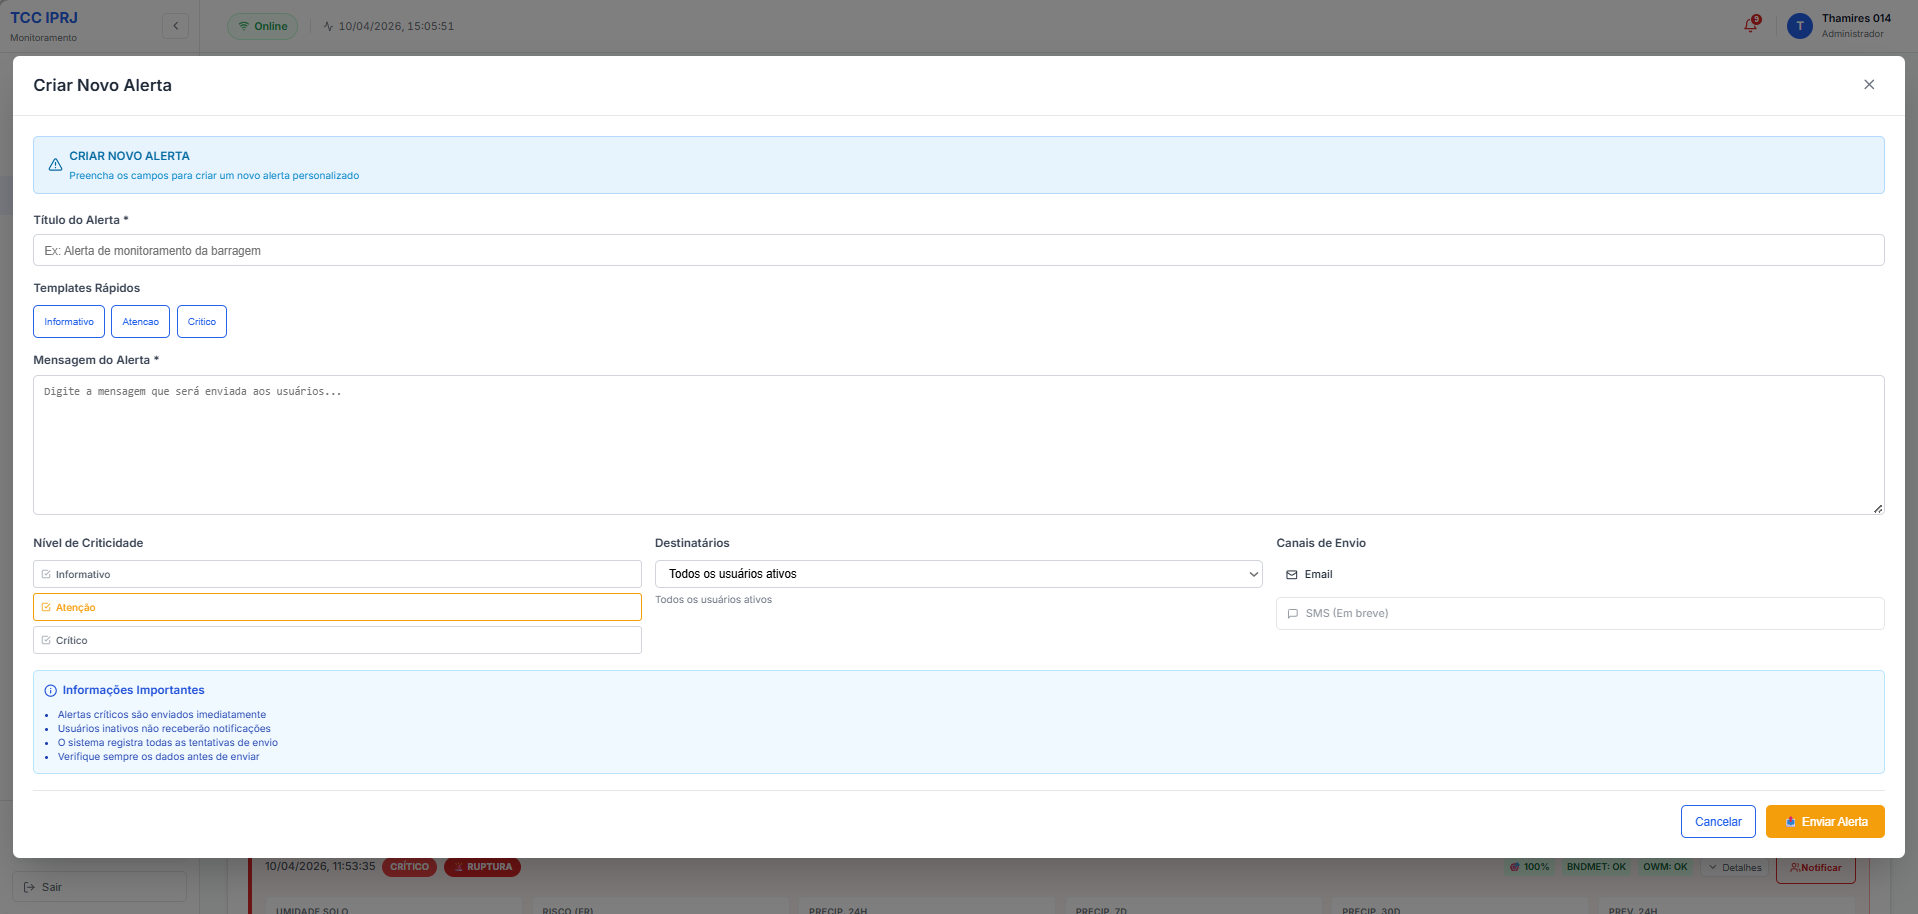
\includegraphics[width=0.80\textwidth]{figures/cap5_alertas_formulario.png}
    \caption{Formulário de envio de alerta manual: campos de título,
    mensagem, nível de criticidade, tipo de destinatário e botões de
    \textit{template} pré-definidos.}
    \label{fig:alertas_formulario}
    \fonte{Elaborado pela autora.}
\end{figure}

Ao confirmar o envio, o sistema processa os destinatários elegíveis e
exibe o \textit{toast} ``Alerta enviado: X sucessos e 0 falhas. Verifiquue os logs para detalhes.'', conforme ilustra a \autoref{fig:alertas_sucesso}. Quando nenhum
destinatário é encontrado para os critérios selecionados --- por exemplo,
se nenhum usuário básico tiver notificações habilitadas ---, o
\textit{backend} retorna erro e o sistema exibe uma mensagem de alerta
sem fechar o modal, permitindo que o administrador ajuste os critérios
e tente novamente, conforme ilustra a \autoref{fig:alertas_sem_destinatario}, e o registro detalhado por
destinatário fica disponível nos logs do sistema.

\begin{figure}[htbp]
    \centering
    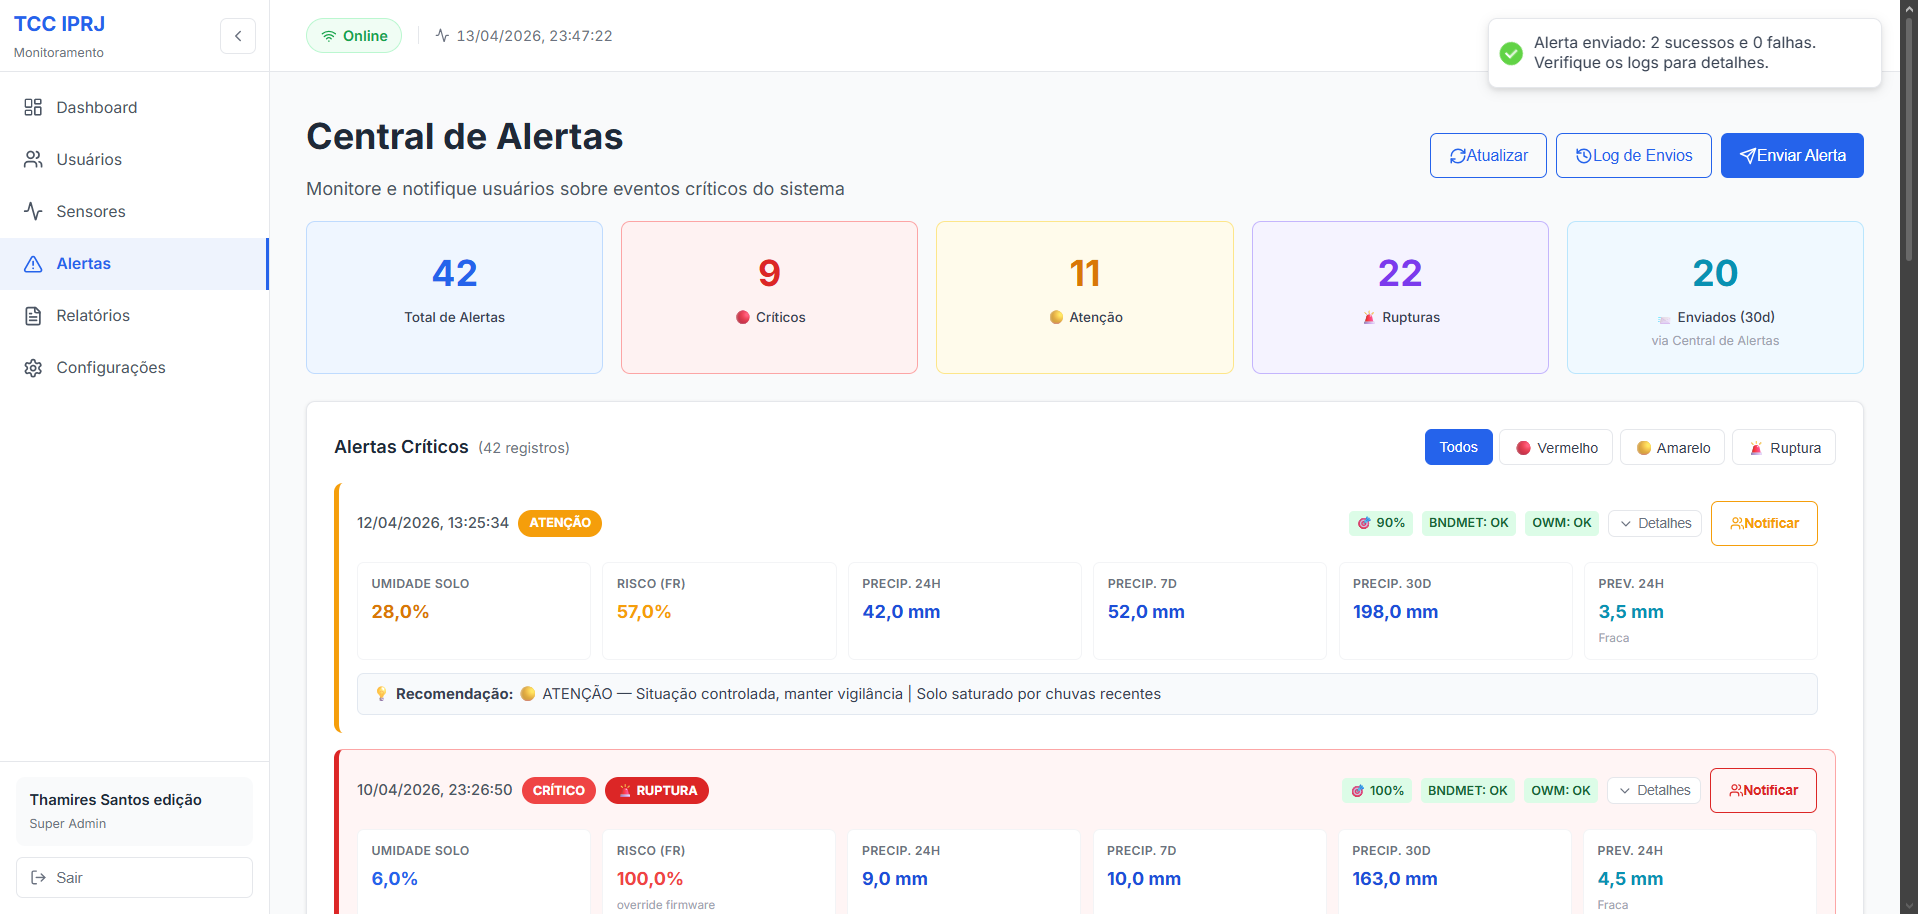
\includegraphics[width=0.80\textwidth]{figures/cap5_alertas_sucesso.png}
    \caption{Formulário de envio de alerta com \textit{toast} de sucesso: confirmação discrimina sucessos e zero falhas.}
    \label{fig:alertas_sucesso}
    \fonte{Elaborado pela autora.}
\end{figure}

\begin{figure}[htbp]
    \centering
    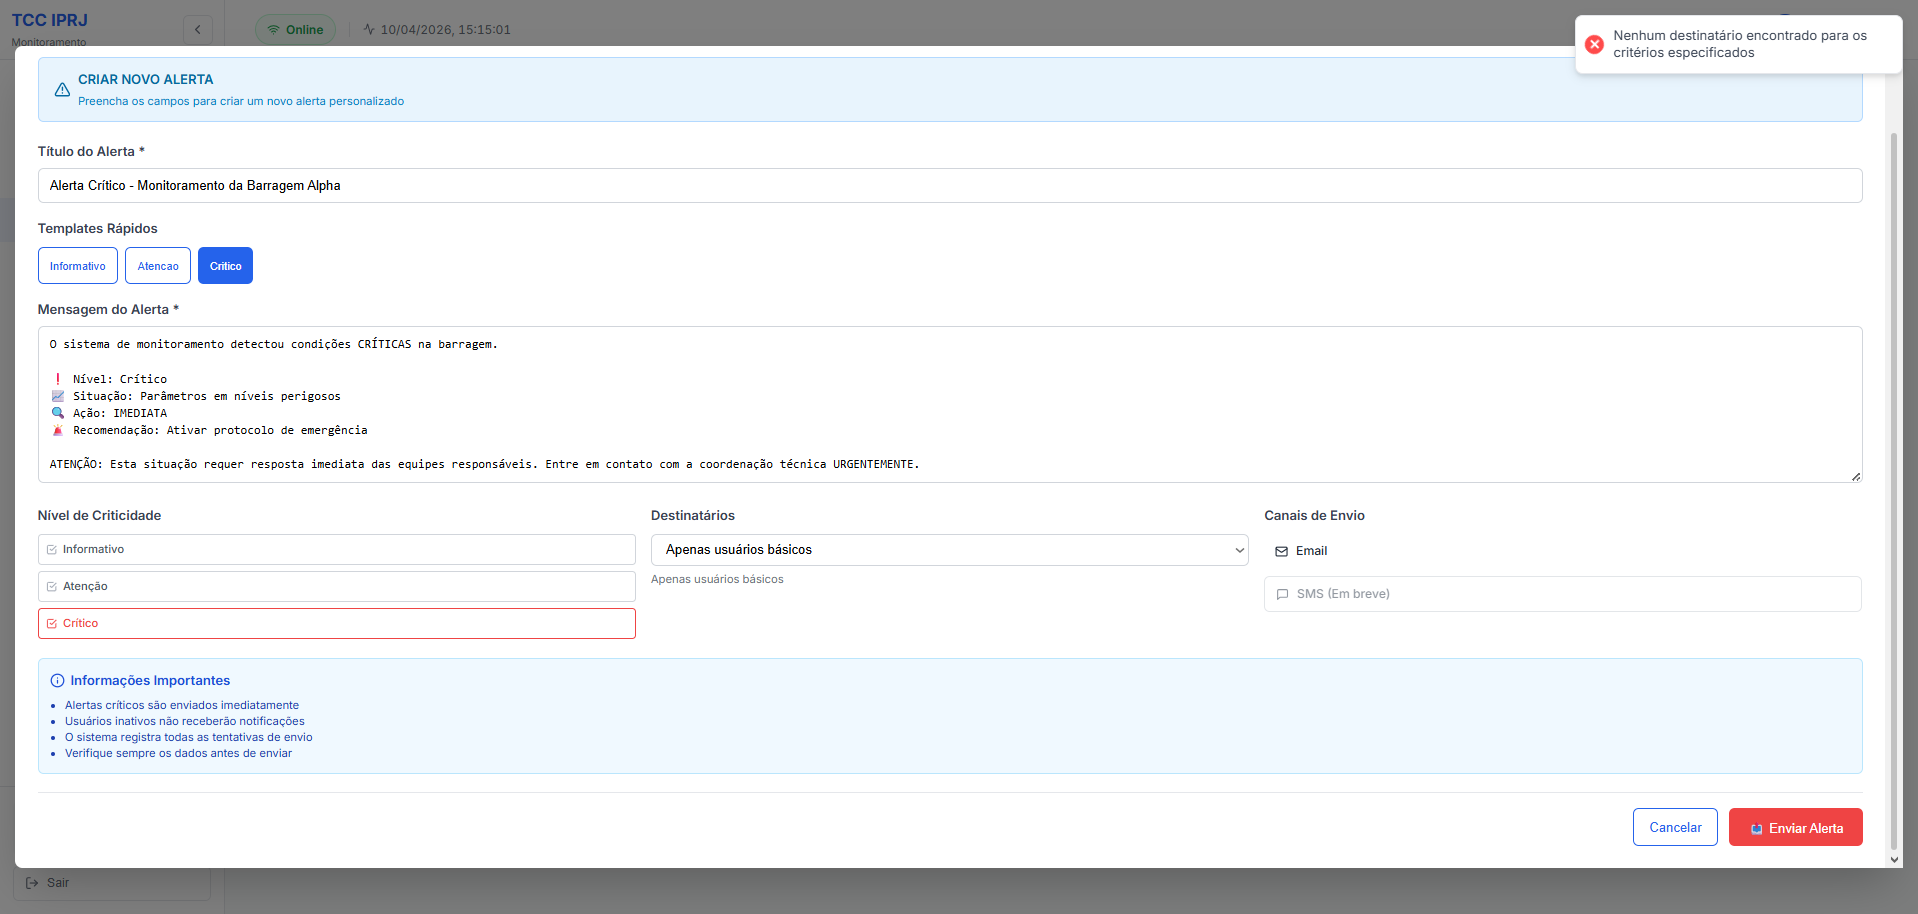
\includegraphics[width=0.80\textwidth]{figures/cap5_alertas_sem_destinatario.png}
    \caption{Formulário de envio de alerta com \textit{toast} de erro por ausência de destinatários: nenhum usuário ativo com notificações habilitadas para os critérios selecionados; modal mantido aberto para ajuste.}
    \label{fig:alertas_sem_destinatario}
    \fonte{Elaborado pela autora.}
\end{figure}

Quando parte das entregas falha, o \textit{toast} de confirmação discrimina sucessos e falhas, conforme ilustram as \autoref{fig:alertas_entrega_parcial_pt1} e \autoref{fig:alertas_entrega_parcial_pt2}.

\begin{figure}[htbp]
    \centering
    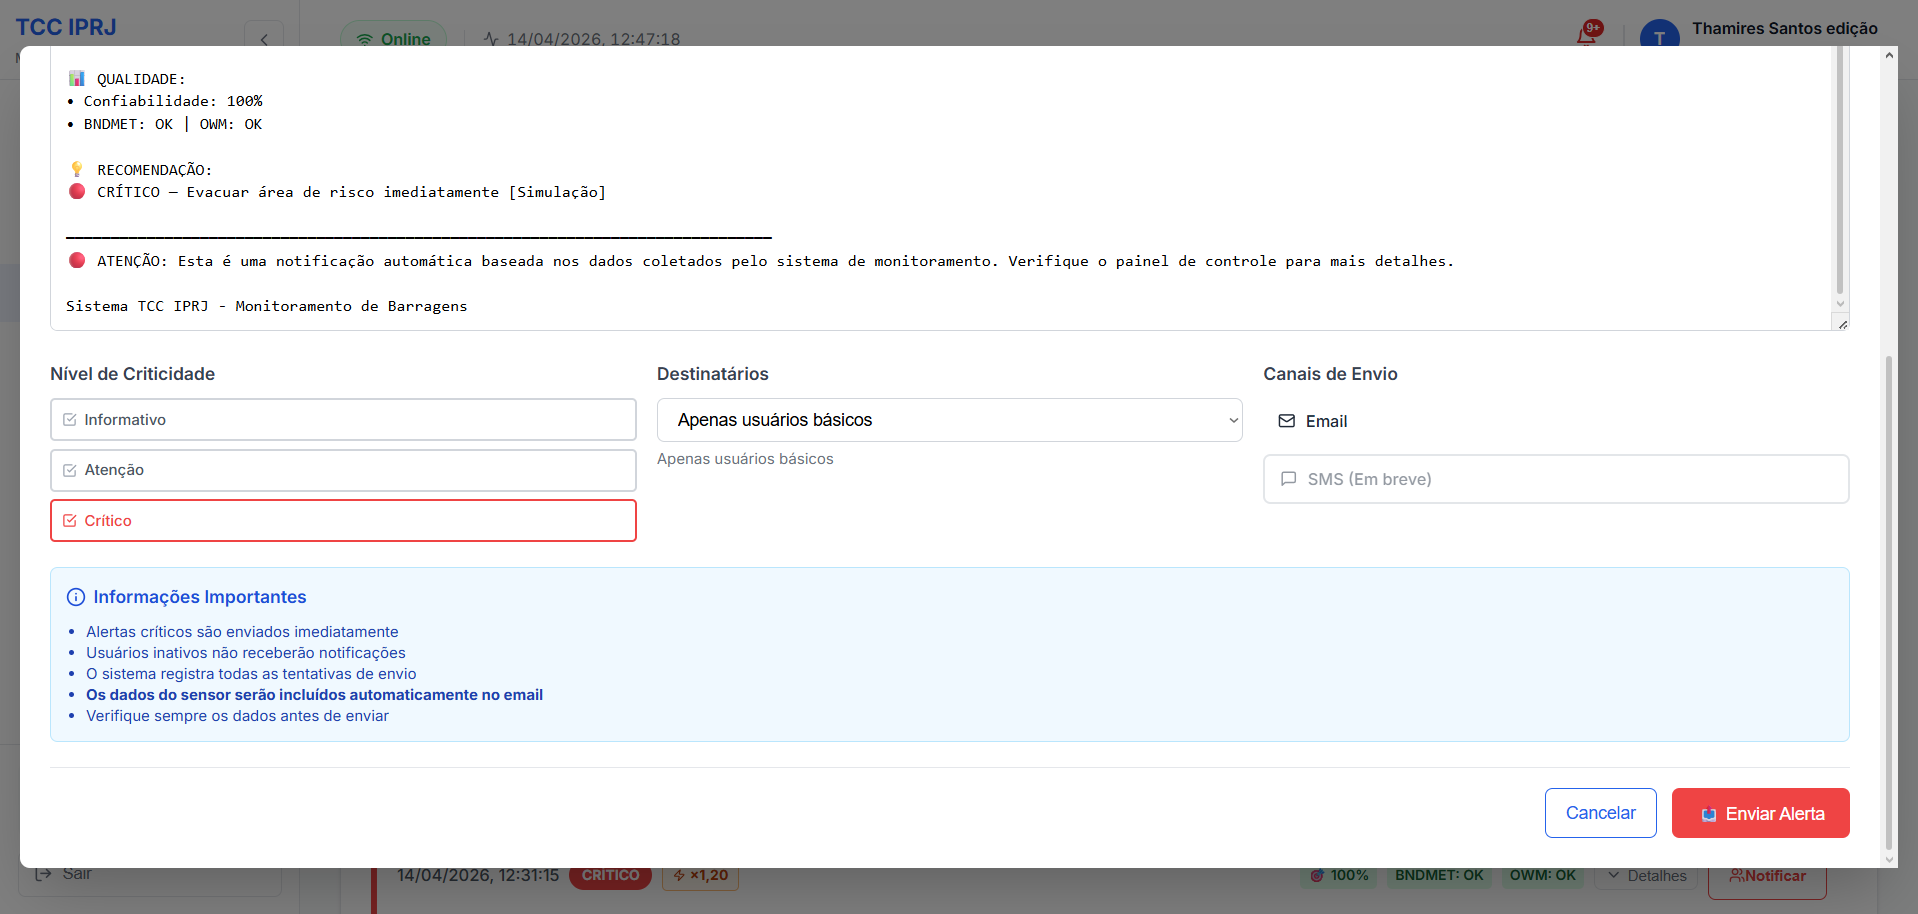
\includegraphics[width=0.80\textwidth]{figures/cap5_alertas_entrega_parcial_pt1.png}
    \caption{Alerta com falhas parciais de entrega (parte~1): destinatários selecionados.}
    \label{fig:alertas_entrega_parcial_pt1}
    \fonte{Elaborado pela autora.}
\end{figure}

\begin{figure}[htbp]
    \centering
    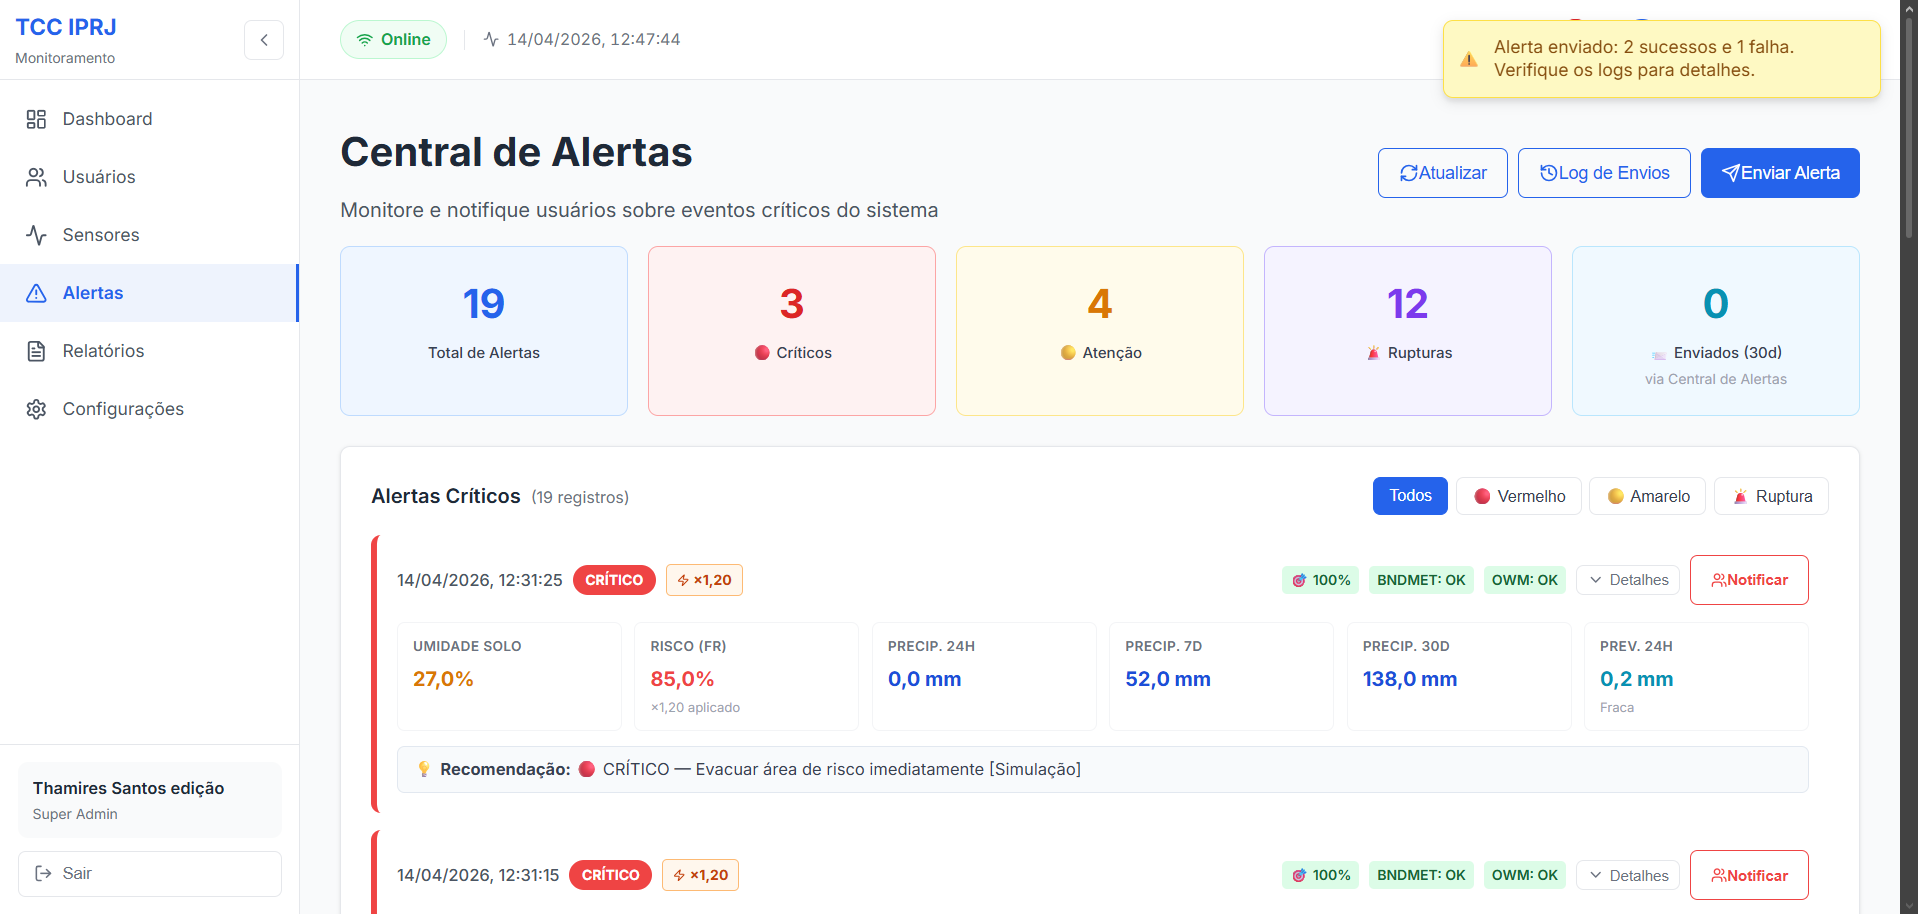
\includegraphics[width=0.80\textwidth]{figures/cap5_alertas_entrega_parcial_pt2.png}
    \caption{\textit{Toast} de confirmação de envio de alerta com falhas parciais de entrega (parte~2): número de e-mails enviados com sucesso e falha.}
    \label{fig:alertas_entrega_parcial_pt2}
    \fonte{Elaborado pela autora.}
\end{figure}

% -------------------------------------------------------------
\subsection{Recebimento do E-mail de Alerta}
\label{subsec:alertas-email}
% -------------------------------------------------------------

O destinatário recebe um e-mail HTML com cabeçalho colorido conforme o
nível de criticidade --- verde para baixo, amarelo para médio e vermelho
para crítico --- como mostram as \autoref{fig:email_recebido_pt1} a
\autoref{fig:email_recebido_pt3}. O corpo do e-mail apresenta o título,
a mensagem composta pelo administrador, a data e hora no fuso horário de
Brasília e o rodapé de identificação do sistema, conforme ilustra a
\autoref{fig:email_recebido_pt4}.

Falhas síncronas de entrega SMTP --- como endereços com formato inválido,
rejeitados pelo próprio \textit{Nodemailer} antes do envio --- são
detectadas imediatamente pelo \textit{backend}, registradas individualmente
em \texttt{logs\_alertas} e contabilizadas no \textit{toast} de confirmação
exibido ao administrador, conforme ilustra a
\autoref{fig:alertas_entrega_parcial_pt2}, sem interromper os demais envios
do lote. Após recarregar a tela, a lista de alertas críticos reflete o
estado atualizado do sistema, como mostra a
\autoref{fig:email_recebido_pt5}. Falhas assíncronas, como
rejeições por domínio inexistente (\textit{bounce}), ocorrem após o servidor
SMTP aceitar a mensagem: o \textit{backend} registra o envio como
bem-sucedido e a notificação de falha retorna posteriormente à caixa do
remetente, conforme ilustra a \autoref{fig:email_recebido_pt6}, fora do
controle do sistema. Esse comportamento é inerente ao protocolo SMTP e
exigiria integração com serviço especializado de monitoramento de
\textit{bounces} para tratamento automatizado.

\begin{figure}[htbp]
    \centering
    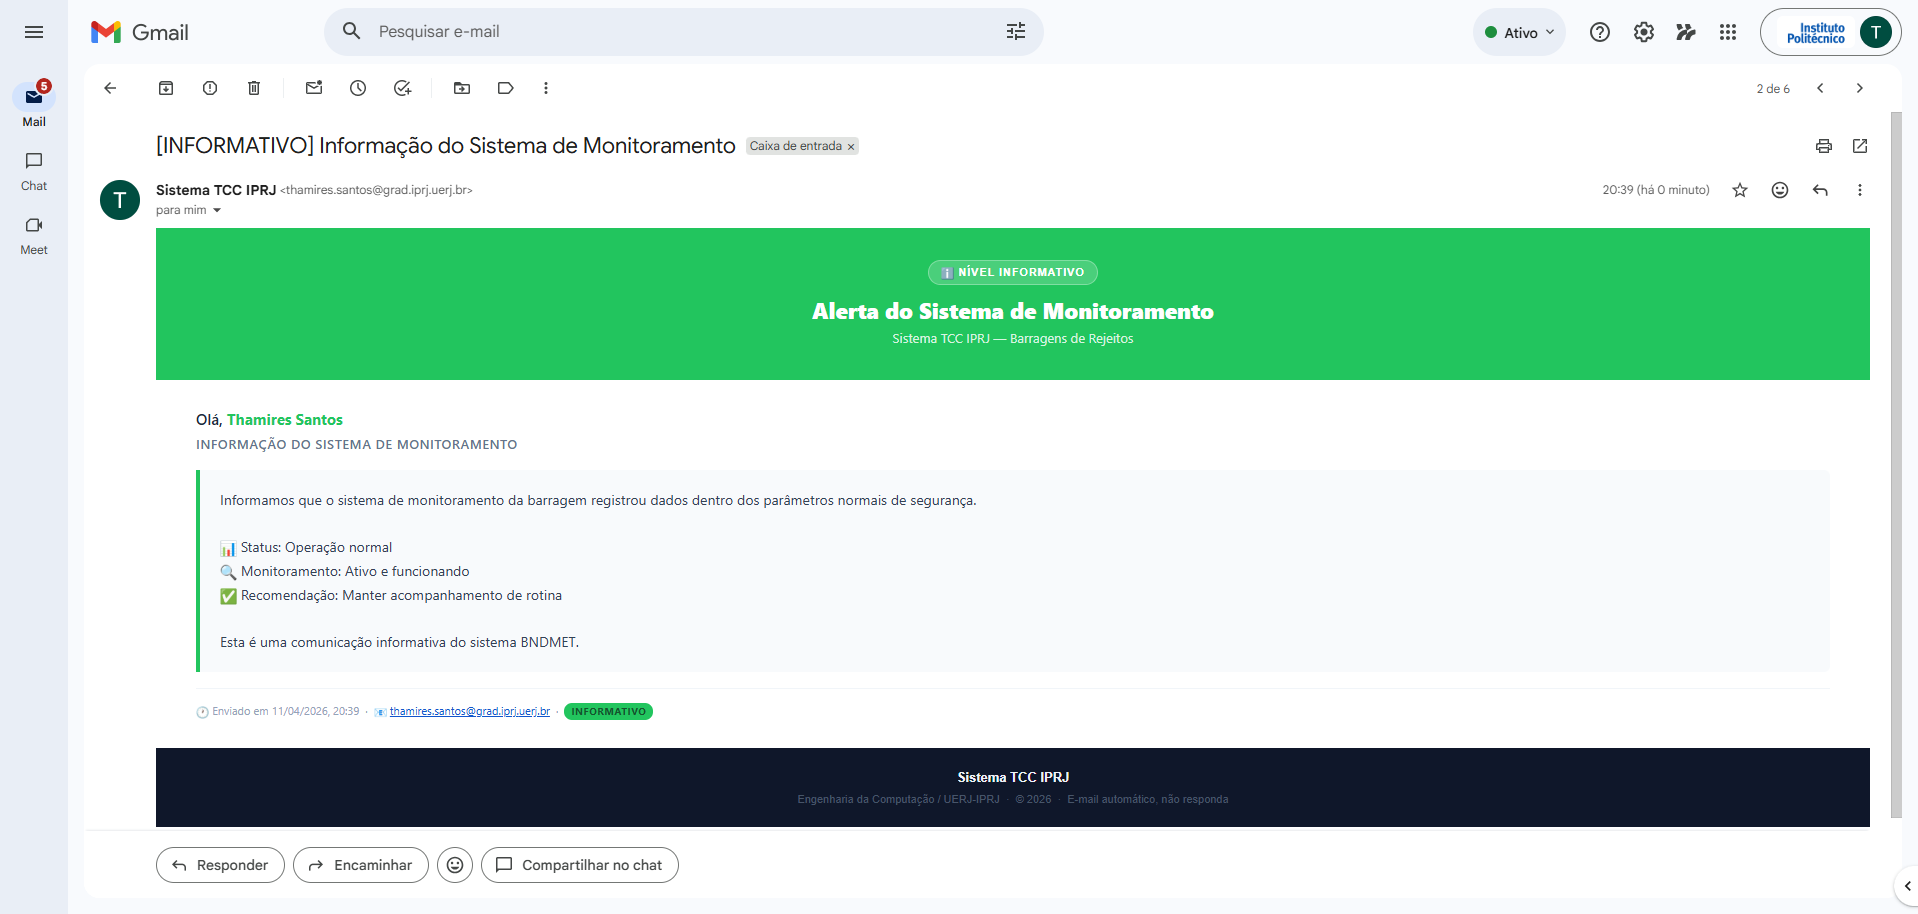
\includegraphics[width=0.80\textwidth]{figures/cap5_email_recebido_pt1.png}
    \caption{E-mail de alerta recebido pelo destinatário (parte~1):
    nível Informativo.}
    \label{fig:email_recebido_pt1}
    \fonte{Elaborado pela autora.}
\end{figure}

\begin{figure}[htbp]
    \centering
    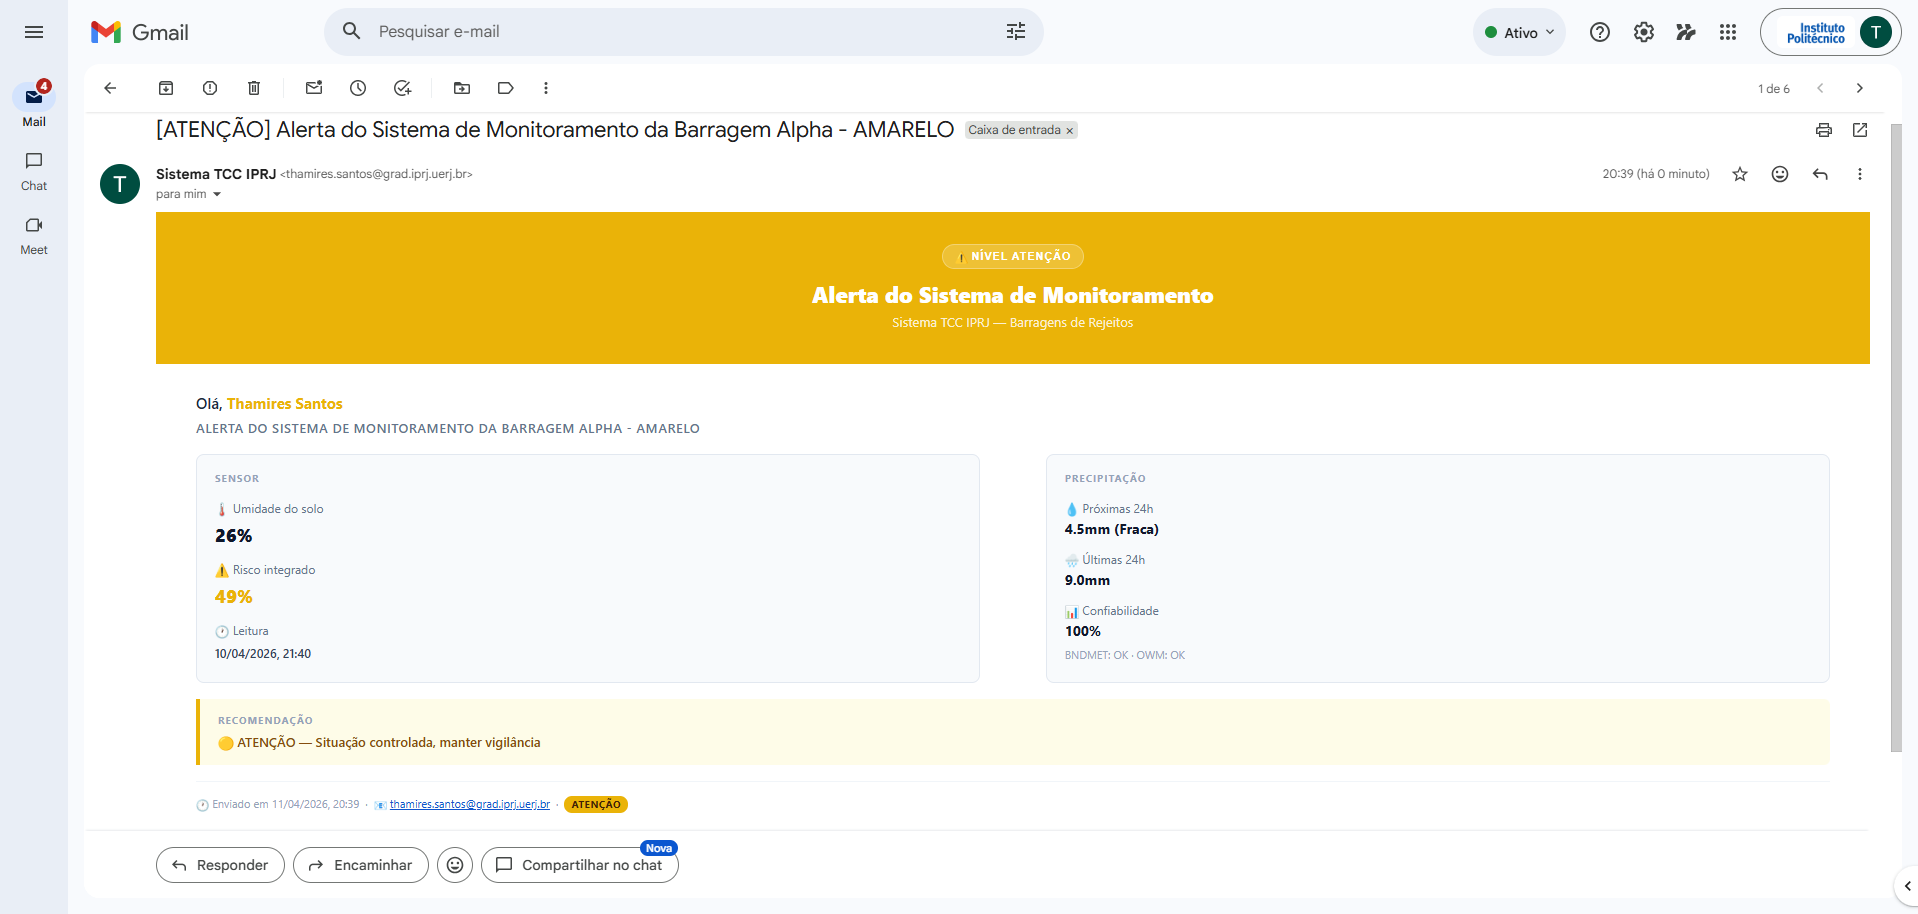
\includegraphics[width=0.80\textwidth]{figures/cap5_email_recebido_pt2.png}
    \caption{E-mail de alerta recebido pelo destinatário (parte~2):
    nível Atenção.}
    \label{fig:email_recebido_pt2}
    \fonte{Elaborado pela autora.}
\end{figure}

\begin{figure}[htbp]
    \centering
    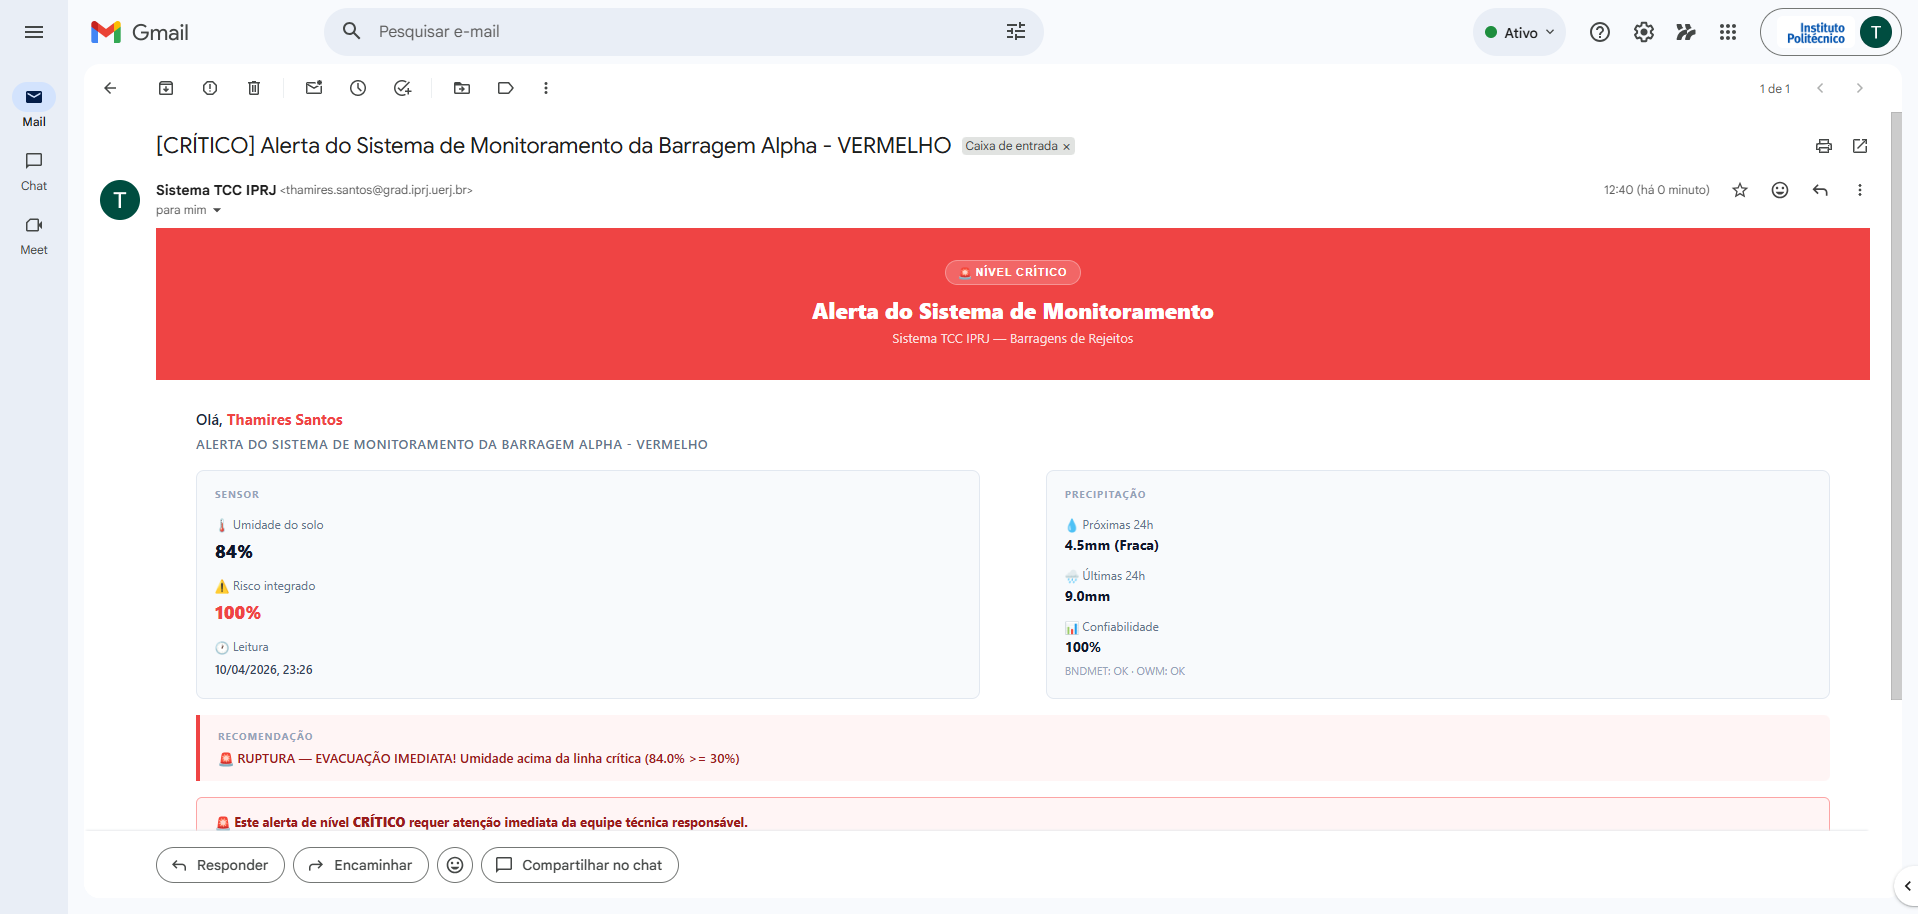
\includegraphics[width=0.80\textwidth]{figures/cap5_email_recebido_pt3.png}
    \caption{E-mail de alerta recebido pelo destinatário (parte~3):
    nível Crítico.}
    \label{fig:email_recebido_pt3}
    \fonte{Elaborado pela autora.}
\end{figure}

\begin{figure}[htbp]
    \centering
    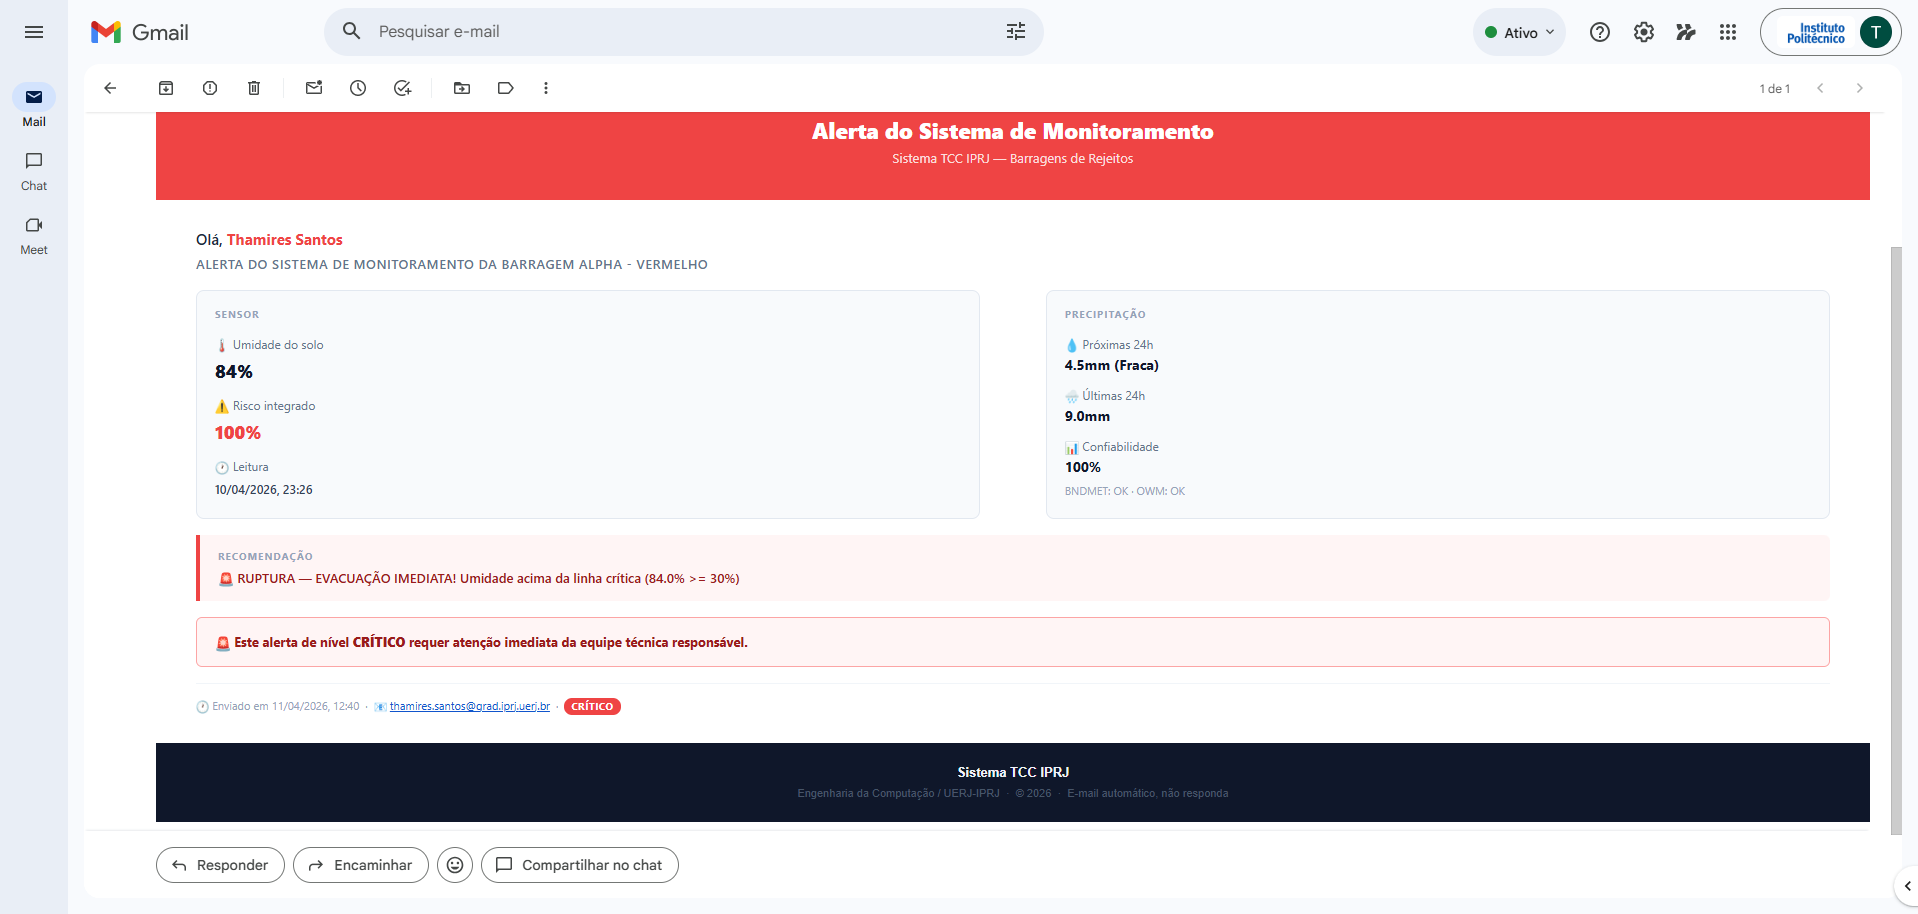
\includegraphics[width=0.80\textwidth]{figures/cap5_email_recebido_pt4.png}
    \caption{E-mail de alerta recebido pelo destinatário (parte~4):
    corpo da mensagem composta pelo administrador, data e hora no fuso horário de Brasília e rodapé de identificação
    do sistema.}
    \label{fig:email_recebido_pt4}
    \fonte{Elaborado pela autora.}
\end{figure}

\begin{figure}[htbp]
    \centering
    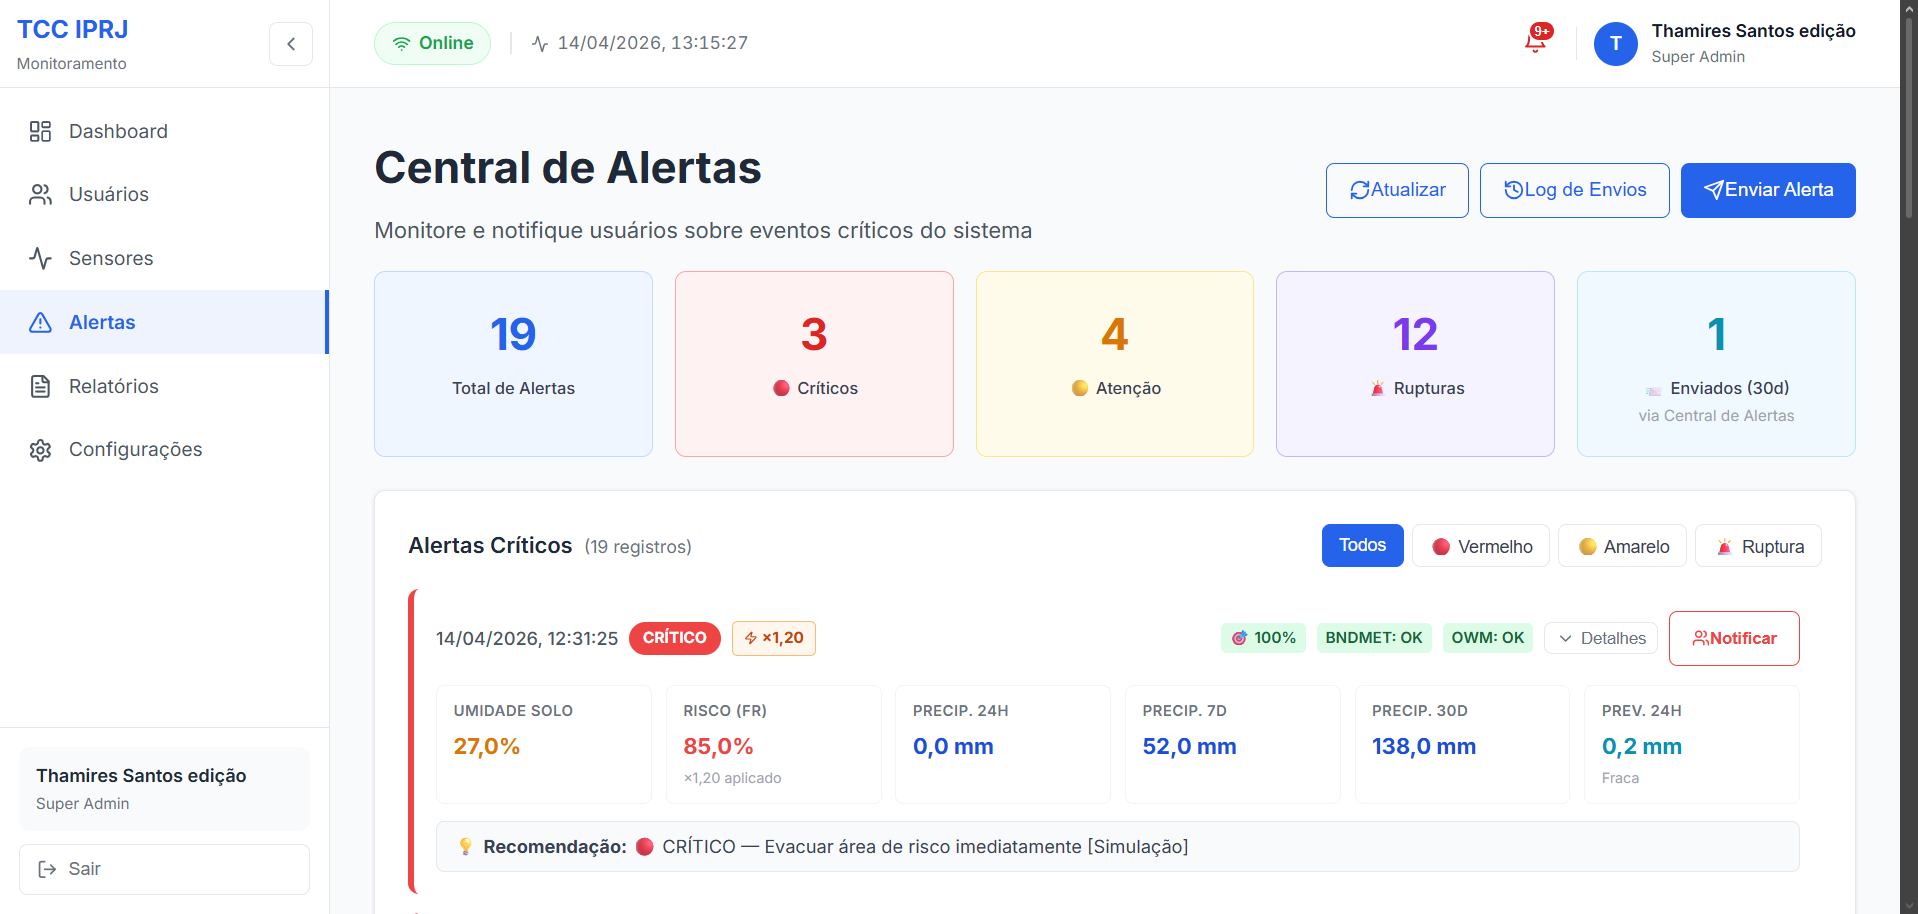
\includegraphics[width=0.95\textwidth]{figures/cap5_email_recebido_pt5.png}
    \caption{Modal ``Log de Alertas Enviados'' (parte~5): Tela de Alertas atualizada (parte~5):
    registradas individualmente em \texttt{logs\_alertas} os sucessos e falhas.}
    \label{fig:email_recebido_pt5}
    \fonte{Elaborado pela autora.}
\end{figure}

\begin{figure}[htbp]
    \centering
    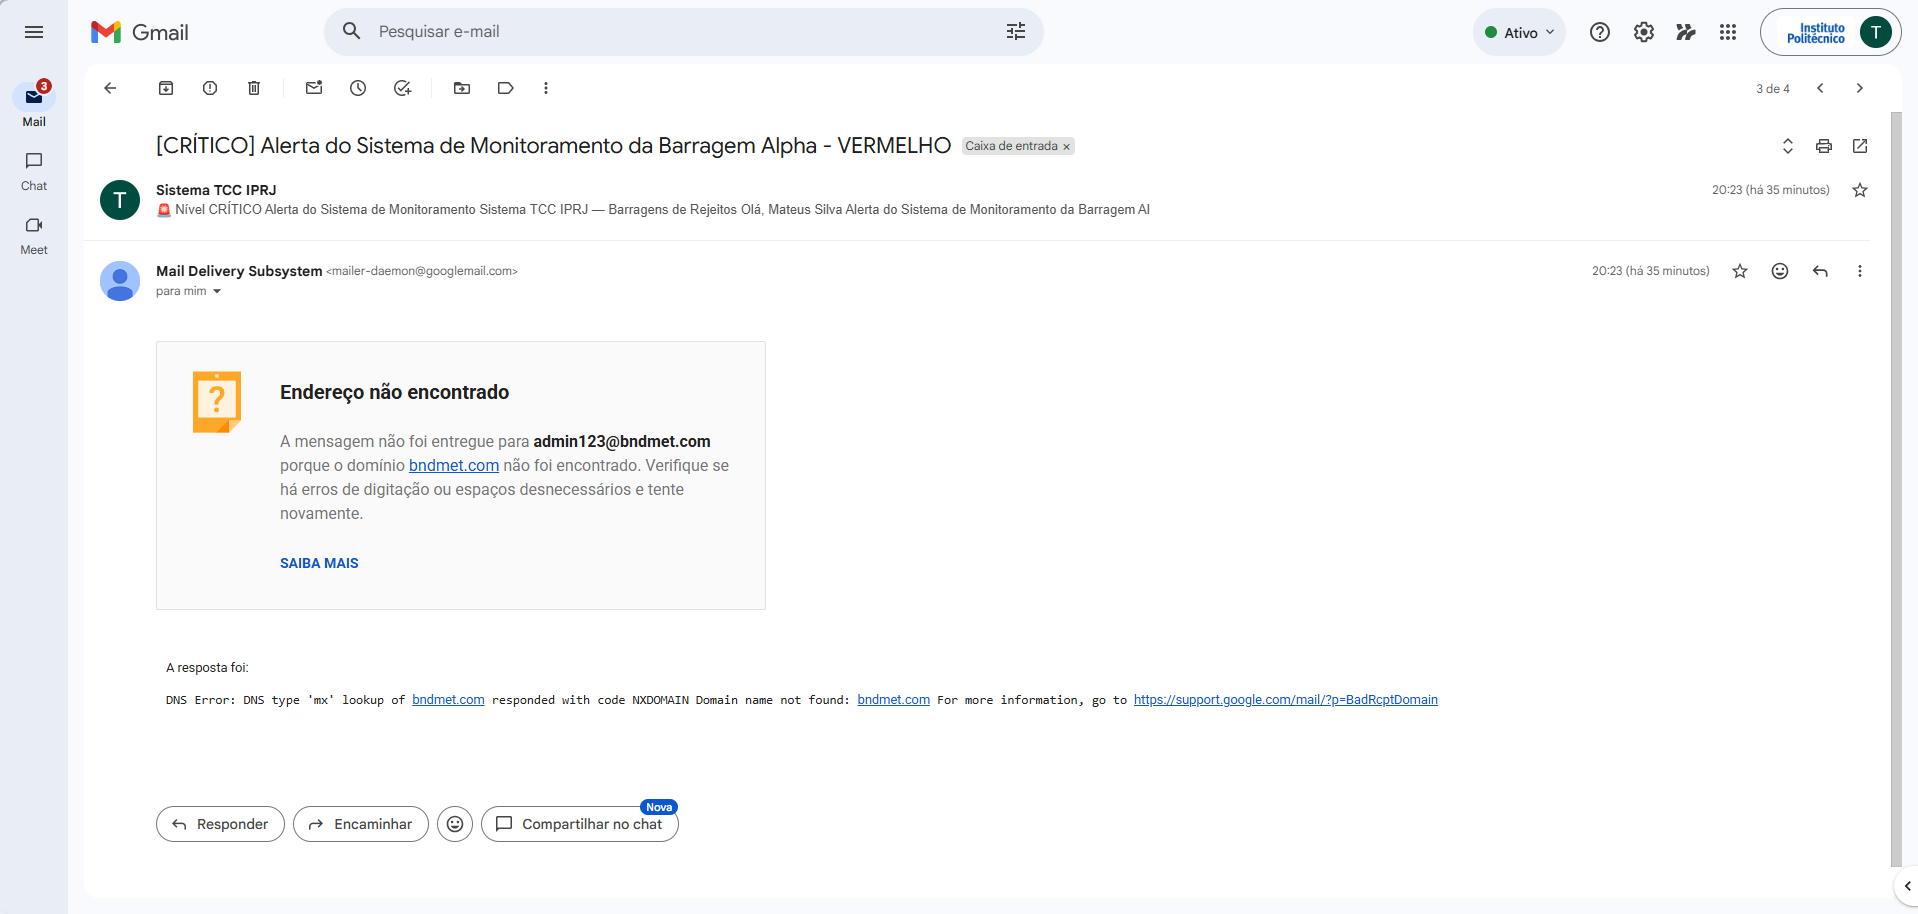
\includegraphics[width=0.80\textwidth]{figures/cap5_email_recebido_pt6.png}
    \caption{E-mail de alerta recebido pelo remetente (parte~6):
    notificação de falha retorna posteriormente à caixa do remetente.}
    \label{fig:email_recebido_pt6}
    \fonte{Elaborado pela autora.}
\end{figure}

% -------------------------------------------------------------
\subsection{Log de Alertas Enviados}
\label{subsec:alertas-log}
% -------------------------------------------------------------

O botão ``Log de Envios'', posicionado no cabeçalho da tela de Alertas
ao lado dos botões ``Atualizar'' e ``Enviar Alerta'', abre um modal com
o histórico completo de alertas disparados pela Central de Alertas. Ao
ser acionado, o \textit{frontend} consulta o endpoint
\path{GET /auth/logs-alertas} e exibe os registros da tabela
\texttt{logs\_alertas} em ordem decrescente de data e hora, paginados
a dez por página. A \autoref{fig:alertas_log} mostra o modal com a
tabela de registros.

\begin{figure}[htbp]
    \centering
    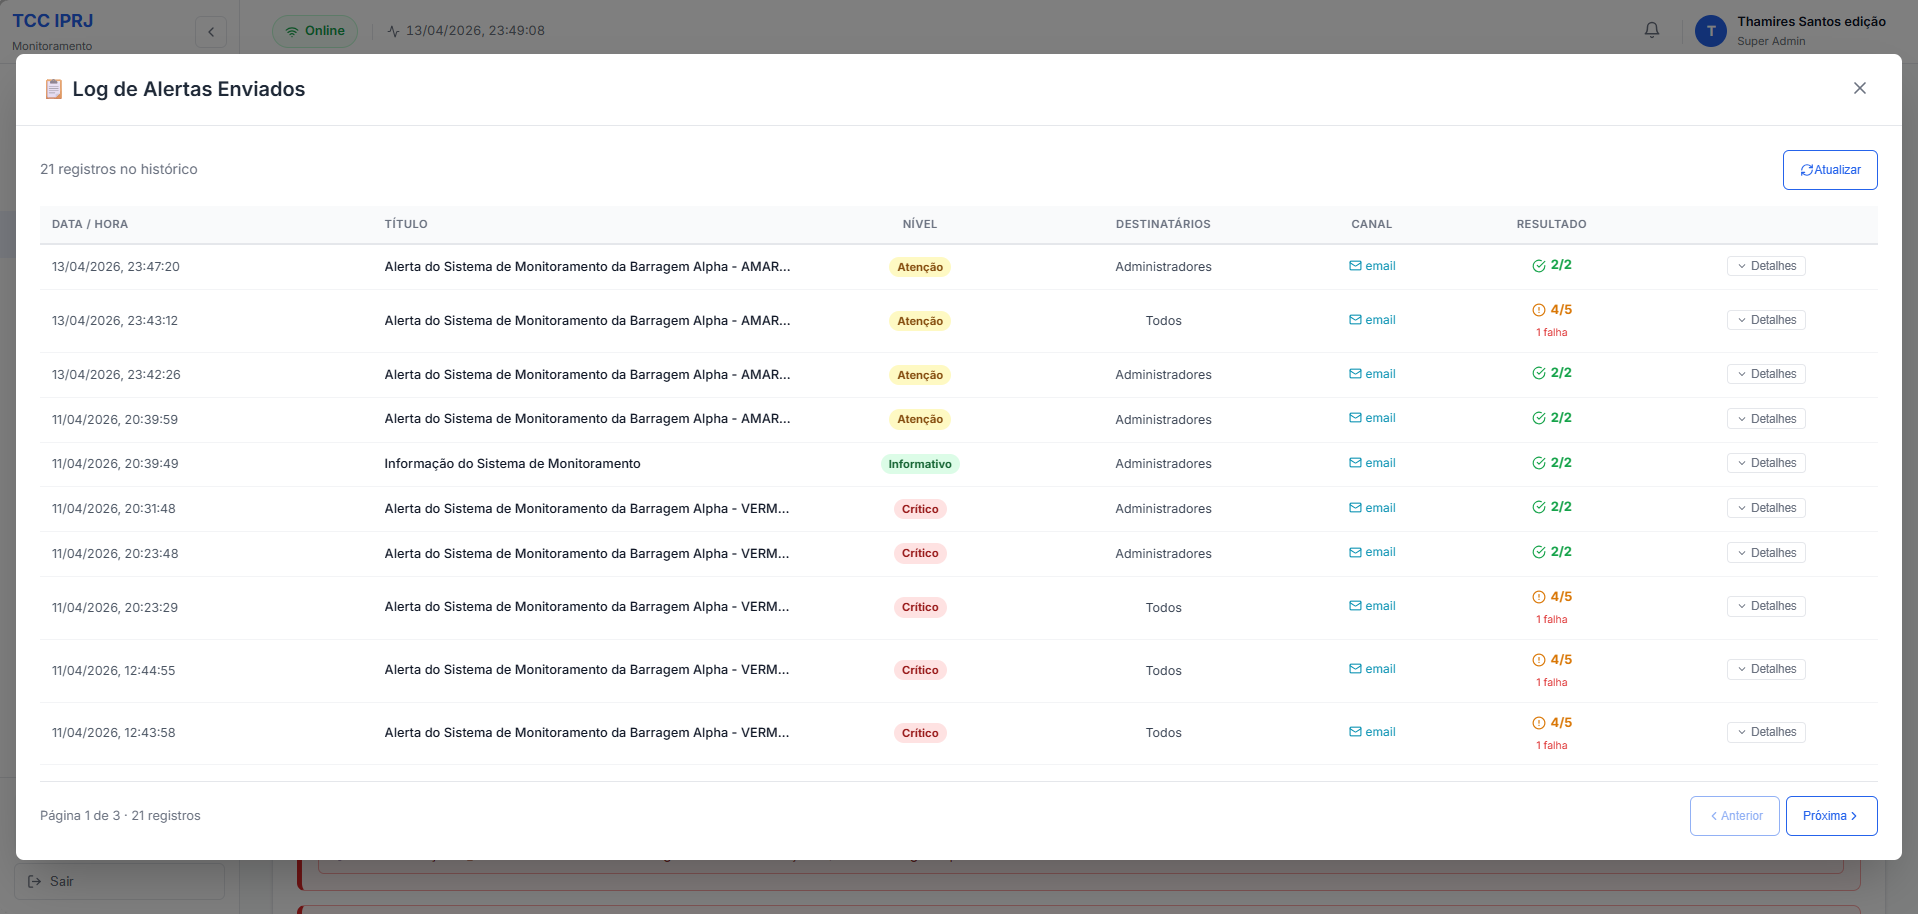
\includegraphics[width=0.95\textwidth]{figures/cap5_alertas_log.png}
    \caption{Modal ``Log de Alertas Enviados'': tabela paginada com
    data e hora, título, nível de criticidade, tipo de destinatário,
    canal e resultado discriminado por sucessos e falhas.}
    \label{fig:alertas_log}
    \fonte{Elaborado pela autora.}
\end{figure}

Cada linha da tabela exibe sete colunas: data e hora do disparo,
título do alerta (truncado com \textit{tooltip} ao passar o cursor),
nível de criticidade representado por \textit{badge} colorido
(Informativo, Atenção ou Crítico), tipo de destinatário selecionado
(Todos, Usuários Básicos ou Administradores), canal de envio, e o
resultado do envio indicado pelo par \textit{sucessos}/\textit{total}
com ícone verde quando todos os e-mails foram entregues, amarelo quando
houve entregas parciais e vermelho quando todos falharam. Quando um
registro apresenta falhas, o número de e-mails não entregues é exibido
abaixo do par de contagem.

Ao clicar em ``Detalhes'' em qualquer linha, uma sub-tabela
expande-se imediatamente abaixo, exibindo o resultado individual por
destinatário: nome, endereço de e-mail, status de entrega e, quando
aplicável, a mensagem de erro retornada pelo servidor SMTP. A
\autoref{fig:alertas_log_detalhe} ilustra a linha expandida com os
detalhes de entrega por destinatário.

\begin{figure}[htbp]
    \centering
    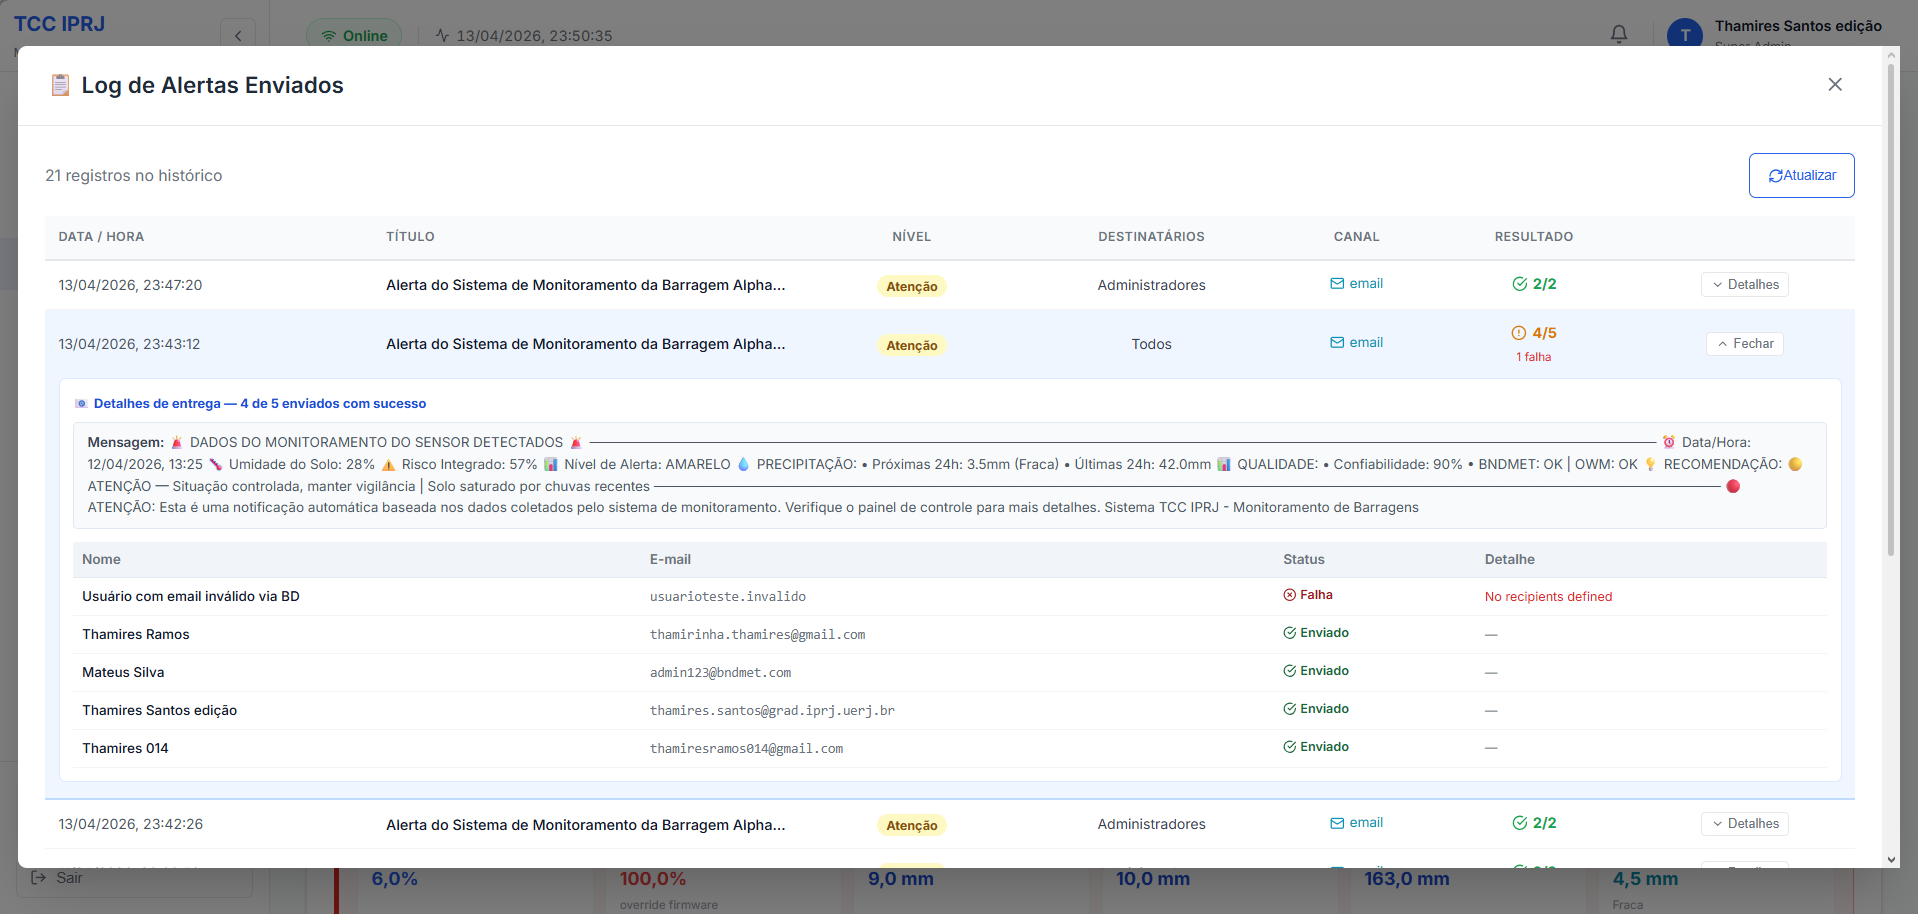
\includegraphics[width=0.95\textwidth]{figures/cap5_alertas_log_detalhe.png}
    \caption{Log de Alertas com linha expandida: sub-tabela de
    detalhes por destinatário exibindo nome, e-mail, status de
    entrega e mensagem de erro quando aplicável.}
    \label{fig:alertas_log_detalhe}
    \fonte{Elaborado pela autora.}
\end{figure}

Quando nenhum alerta foi enviado até o momento, o modal exibe o estado
vazio com a mensagem ``Nenhum alerta foi enviado ainda.''. O botão
``Atualizar'' no cabeçalho do modal recarrega a lista sem necessidade de
fechar e reabrir o painel. Os dados exibidos são somente de leitura e
não alteram nenhum registro no banco de dados, conforme ilustra a
\autoref{fig:alertas_log_vazio}.

\begin{figure}[htbp]
    \centering
    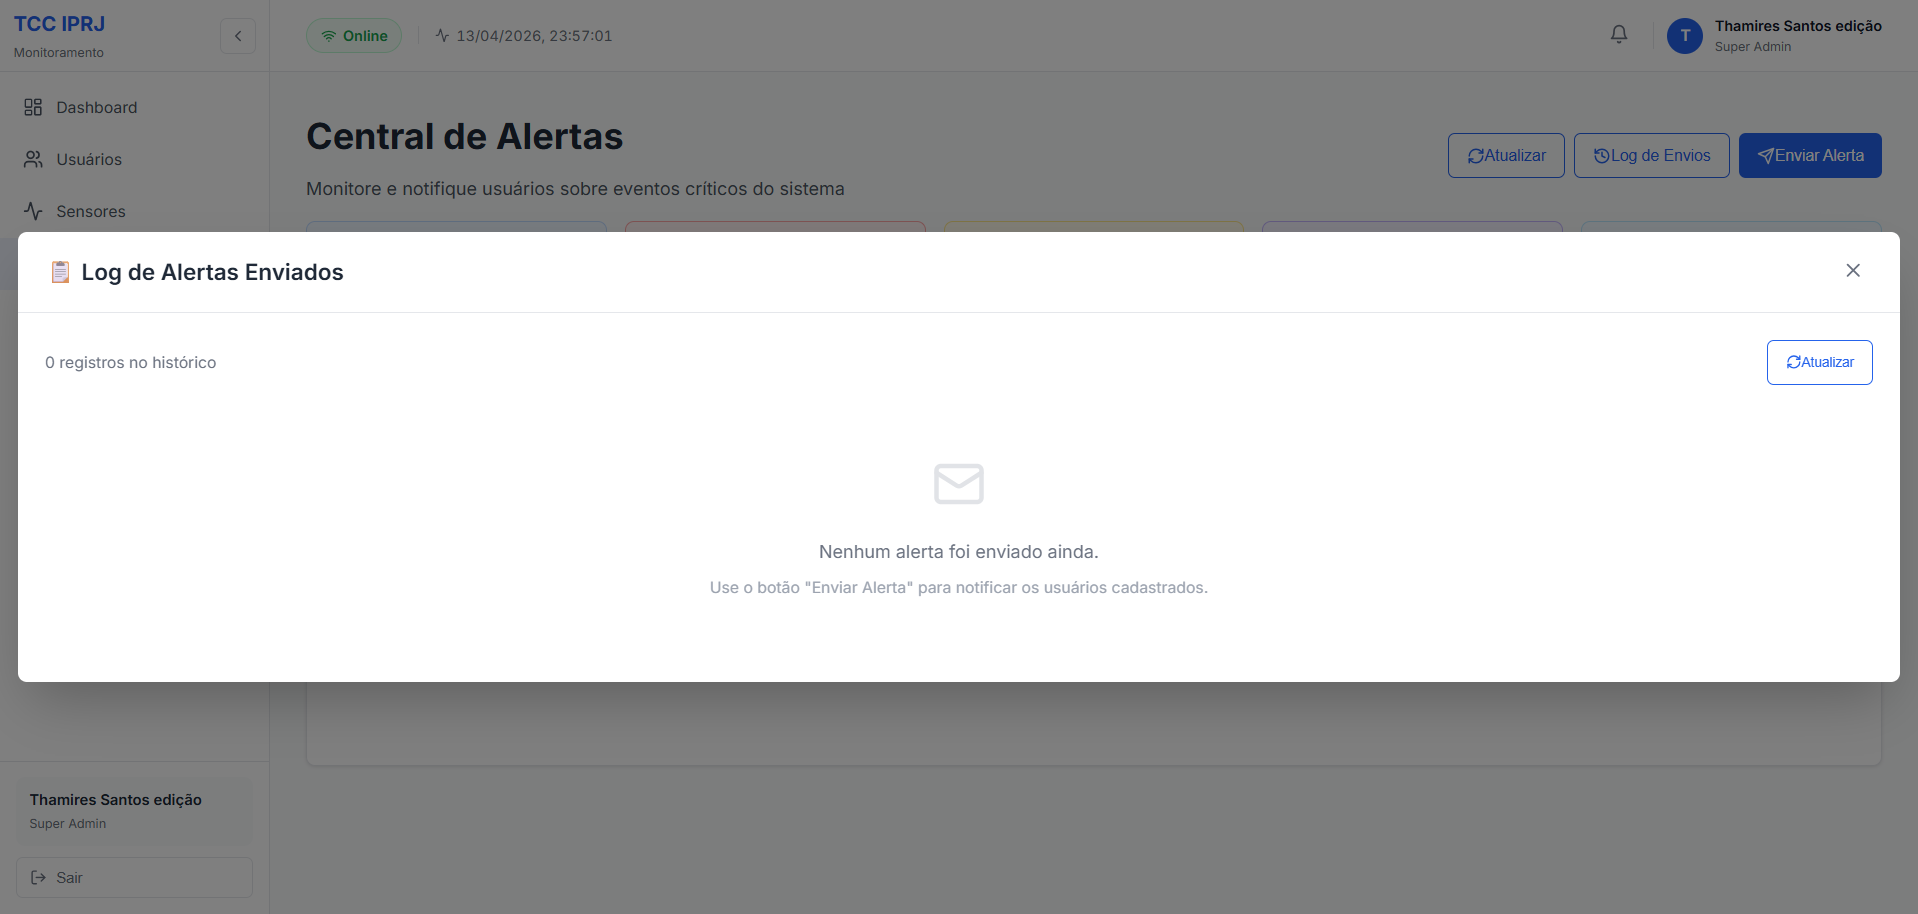
\includegraphics[width=0.95\textwidth]{figures/cap5_alertas_log_vazio.png}
    \caption{Log de Alertas vazio: modal exibe o estado
vazio com a mensagem ``Nenhum alerta foi enviado ainda.''.}
    \label{fig:alertas_log_vazio}
    \fonte{Elaborado pela autora.}
\end{figure}

% =============================================================
\section{Relatórios e Exportações}
\label{sec:relatorios}
% =============================================================

% -------------------------------------------------------------
\subsection{Geração de Relatório por Período}
\label{subsec:relatorio-geracao}
% -------------------------------------------------------------

Ao acessar a tela de Relatórios, o administrador visualiza os
campos de seleção de período --- data de início e data de fim
--- e o botão \textbf{"Gerar Relatório"}, enquanto o sistema
carrega automaticamente o relatório dos últimos sete dias,
conforme ilustra a \autoref{fig:relatorios_estado_inicial}. 

\begin{figure}[htbp]
    \centering
    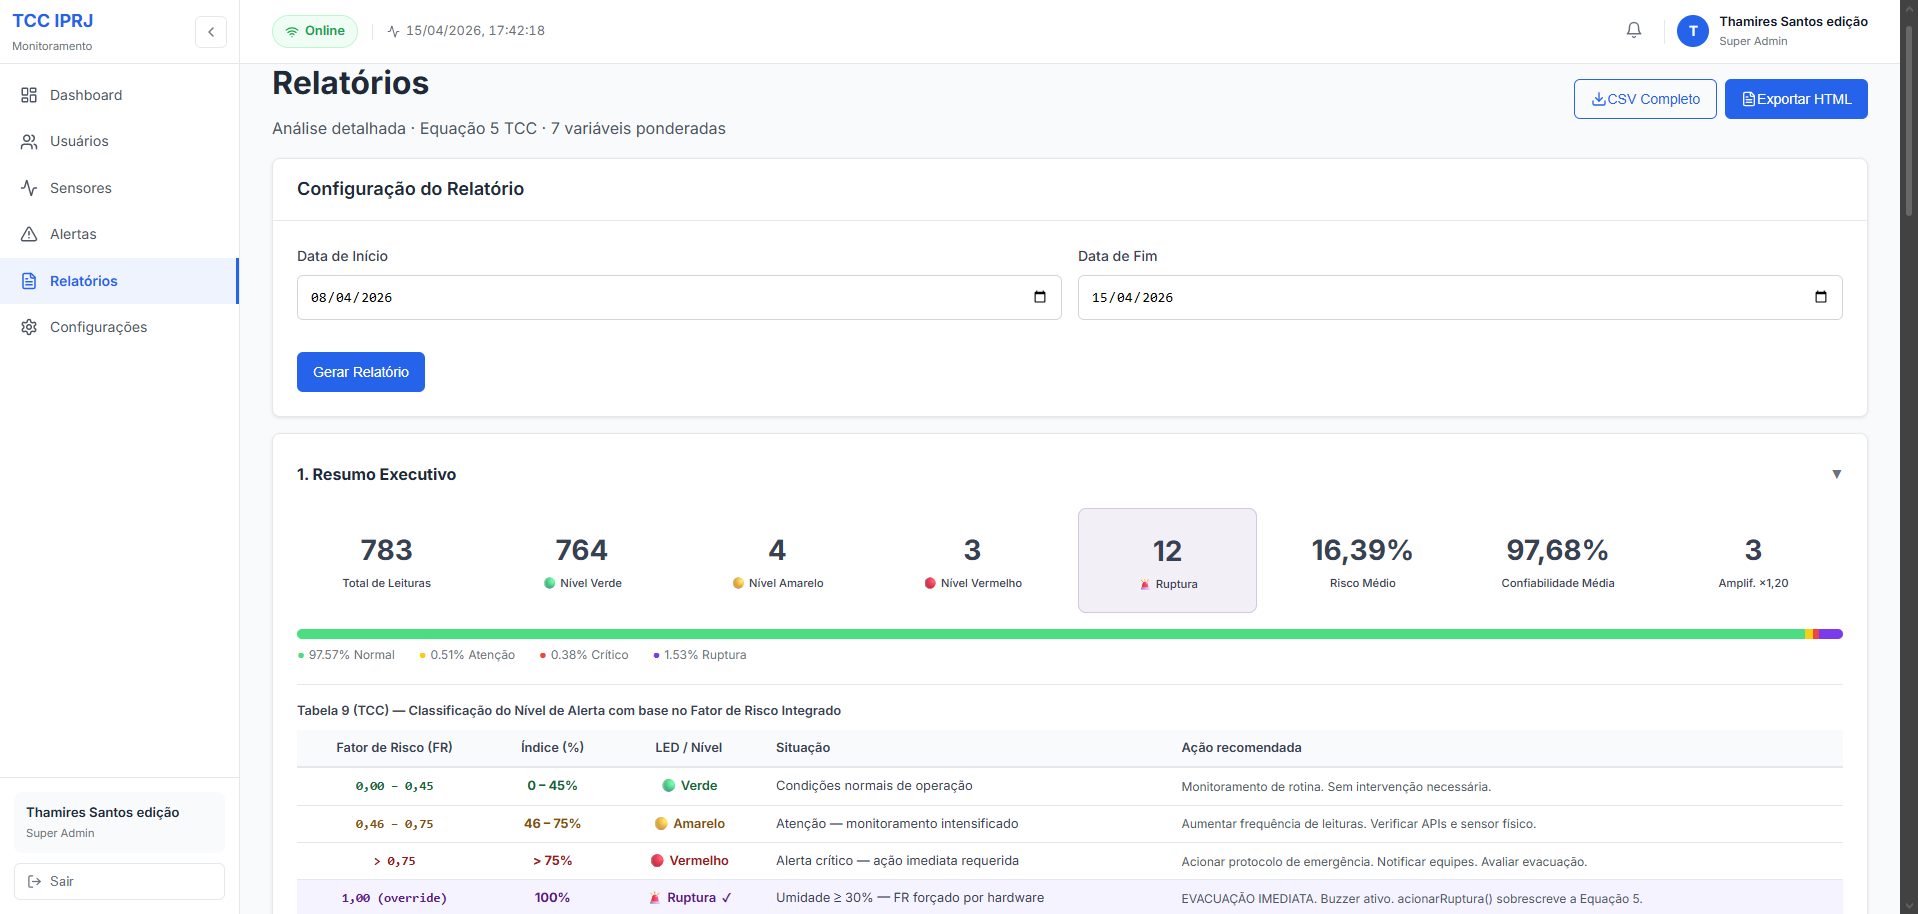
\includegraphics[width=0.85\textwidth]
        {figures/cap5_relatorios_estado_inicial.png}
    \caption{Tela de Relatórios ao ser aberta: campos de seleção
    de período disponíveis e relatório padrão dos últimos sete
    dias carregado automaticamente pelo sistema.}
    \label{fig:relatorios_estado_inicial}
    \fonte{Elaborado pela autora.}
\end{figure}

Para redefinir o intervalo de análise, o administrador informa
as datas de início e fim e clica em \textbf{"Gerar Relatório"};
o relatório atualizado é exibido nas seis seções colapsáveis,
conforme ilustram as \autoref{fig:relatorio_gerado_pt1} a
\autoref{fig:relatorio_gerado_pt6}.

\begin{figure}[htbp]
    \centering
    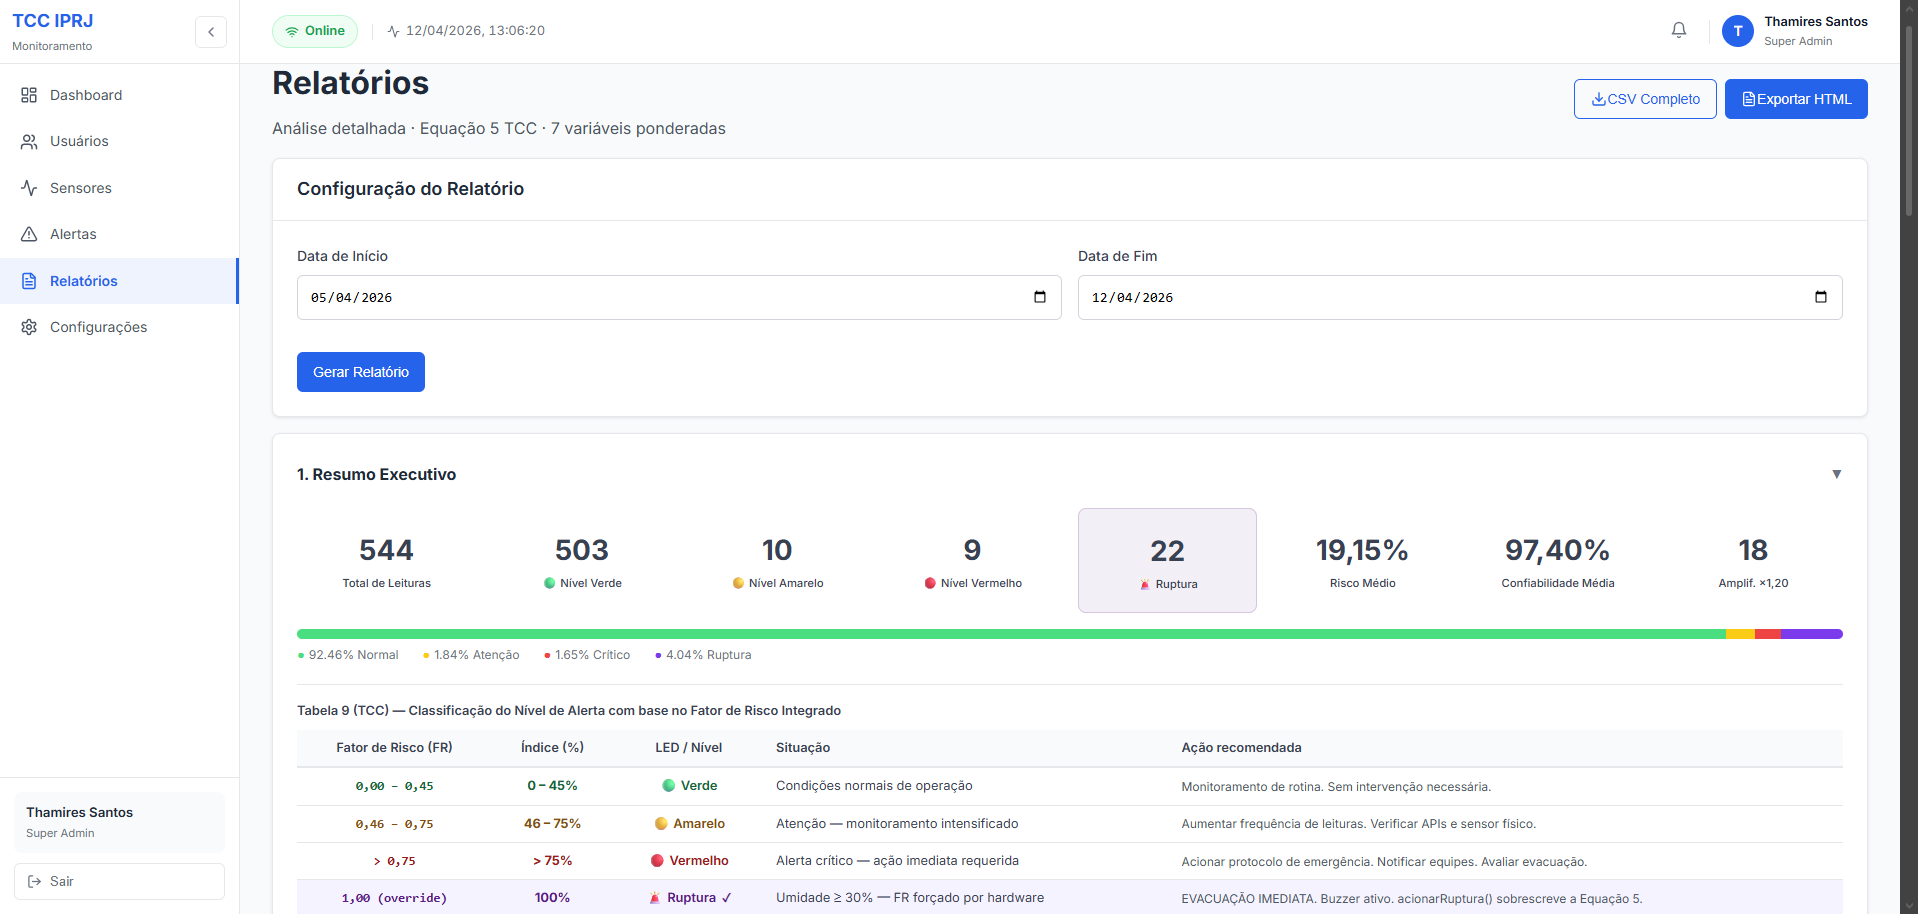
\includegraphics[width=0.95\textwidth]{figures/cap5_relatorio_gerado_pt1.png}
    \caption{Tela de Relatórios com relatório gerado (parte~1): configuração
    do período e seção Resumo Executivo com KPIs de contagem por nível de
    alerta, risco médio, confiabilidade média, eventos com amplificação
    ativa e barra proporcional de distribuição.}
    \label{fig:relatorio_gerado_pt1}
    \fonte{Elaborado pela autora.}
\end{figure}

O relatório é organizado em seis seções colapsáveis. A primeira, Resumo
Executivo, exibe o total de leituras do período e oito KPIs: contagens por
nível de alerta --- Normal, Atenção, Crítico e Ruptura ---, risco médio,
confiabilidade média e número de eventos com amplificação ×1,20 ativa.
Uma barra proporcional colore a distribuição percentual por nível e, abaixo
dela, a Tabela~9~TCC apresenta os limiares do fator de risco integrado com
os níveis, situações e ações recomendadas correspondentes, como
ilustra a \autoref{fig:relatorio_gerado_pt1}.

A segunda seção, Dados Meteorológicos e Pluviométricos, organiza os valores
médios do período em duas colunas: à esquerda, precipitações históricas via
BNDMET/DECEA --- acumulados de 24~horas, 7~dias e 30~dias, e precipitação
horária atual pelo fenômeno I175 ---; à direita, condições e previsão via
OpenWeatherMap --- temperatura, umidade relativa do ar, pressão atmosférica
ao nível do solo, velocidade do vento, chuva atual (\textit{rain.1h}) e
previsão acumulada para 24~horas. A seção exibe ainda a Tabela~7~TCC de
classificação da intensidade pluviométrica prevista, com os cinco níveis
(Fraca, Moderada, Forte, Muito Forte e Pancada de Chuva), os intervalos
de acumulado previsto, o fator \textit{ch.fut} correspondente e o valor
resultante de $V_{ch.futura}$, como mostra a
\autoref{fig:relatorio_gerado_pt2}.

A terceira seção, Componentes da Equação~5 TCC, apresenta a fórmula do
fator de risco integrado FR com a definição de cada variável ponderada,
os intervalos válidos de cada componente, a regra de amplificação ×1,20 e
a condição de ruptura imediata. A tabela exibe, para cada um dos sete
componentes individuais --- $V_{lençol}$, $V_{ch.24h}$, $V_{ch.7d}$,
$V_{ch.30d}$, $V_{ch.futura}$, $V_{taxa}$ e $V_{pressão}$ ---, a fonte
de dado, o valor mínimo, a média e o máximo observados no período, e o
intervalo válido do componente, conforme ilustra a
\autoref{fig:relatorio_gerado_pt3}.

A quarta seção, Qualidade Técnica do Sistema, organiza os indicadores em
duas colunas. À esquerda, Disponibilidade das Fontes informa os percentuais
de operação do sensor ESP8266, da API BNDMET, da qualidade média dos dados
BNDMET, da API OWM, da conectividade Wi-Fi e o código da estação
pluviométrica consultada. À direita, Eventos e Limites registra as
contagens de acionamentos de amplificação ×1,20, de ciclos com
\textit{buzzer} ativo e de registros em modo manual, além dos valores
mínimo e máximo de risco e de confiabilidade observados no período. A
quinta seção, Diagnóstico de Hardware ESP8266, divide-se em Memória ---
com os valores mínimo e médio de memória livre (\textit{freeHeap}) e o
maior tempo de operação contínua --- e Conectividade --- com o RSSI médio
e mínimo do sinal Wi-Fi e as tentativas de envio média e máxima ---, como
mostra a \autoref{fig:relatorio_gerado_pt4}.

A sexta e última seção, Registros do Período, exibe em tabela paginada os
primeiros 20 registros do período, com as colunas \textit{timestamp},
umidade do solo, valor ADC, fator local, índice de risco, nível de alerta,
confiabilidade, e \textit{status} de BNDMET, OWM e sensor. Cada linha pode
ser expandida para revelar os componentes $V_x$ da Equação~5, o diagnóstico
de \textit{hardware} e a recomendação operacional. O rodapé da seção informa
o total de registros do período e recomenda a exportação CSV para acesso
ao conjunto completo com os 41~campos, como demonstram as
\autoref{fig:relatorio_gerado_pt5} e \autoref{fig:relatorio_gerado_pt6}.

\begin{figure}[htbp]
    \centering
    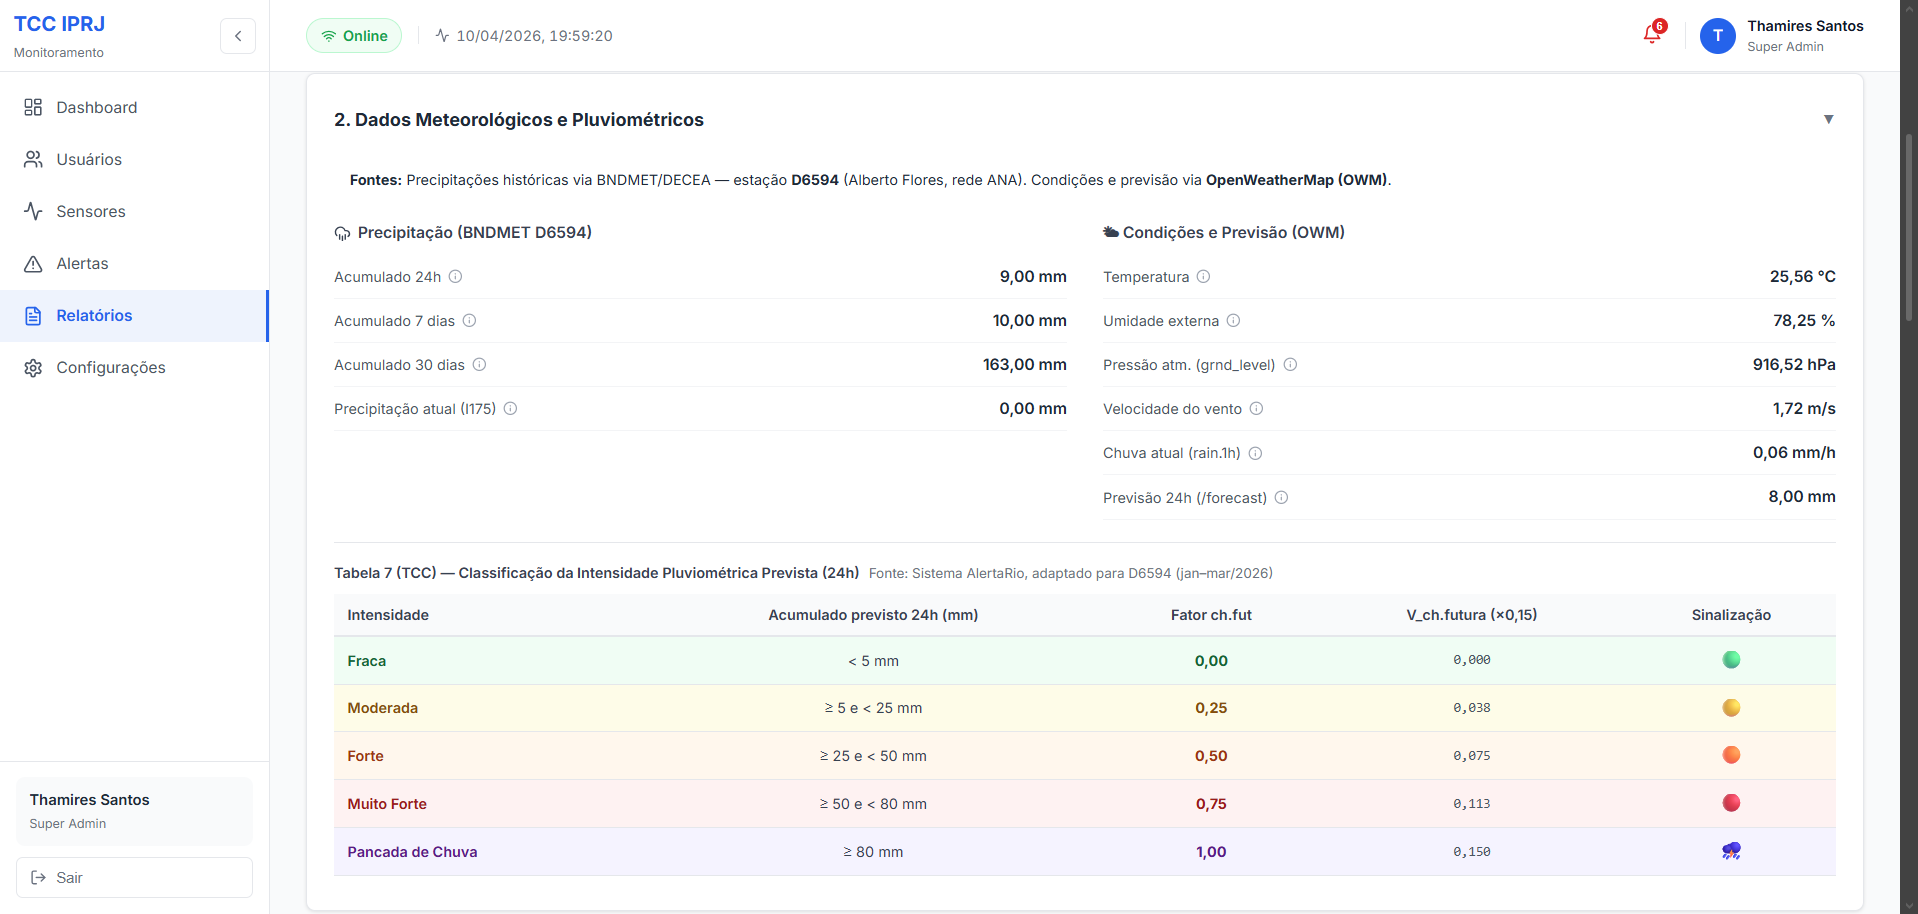
\includegraphics[width=0.95\textwidth]{figures/cap5_relatorio_gerado_pt2.png}
    \caption{Tela de Relatórios com relatório gerado (parte~2): seção
    Dados Meteorológicos e Pluviométricos com valores médios do período
    via BNDMET/DECEA e OpenWeatherMap, e Tabela~7~TCC de classificação
    da intensidade pluviométrica prevista.}
    \label{fig:relatorio_gerado_pt2}
    \fonte{Elaborado pela autora.}
\end{figure}

\begin{figure}[htbp]
    \centering
    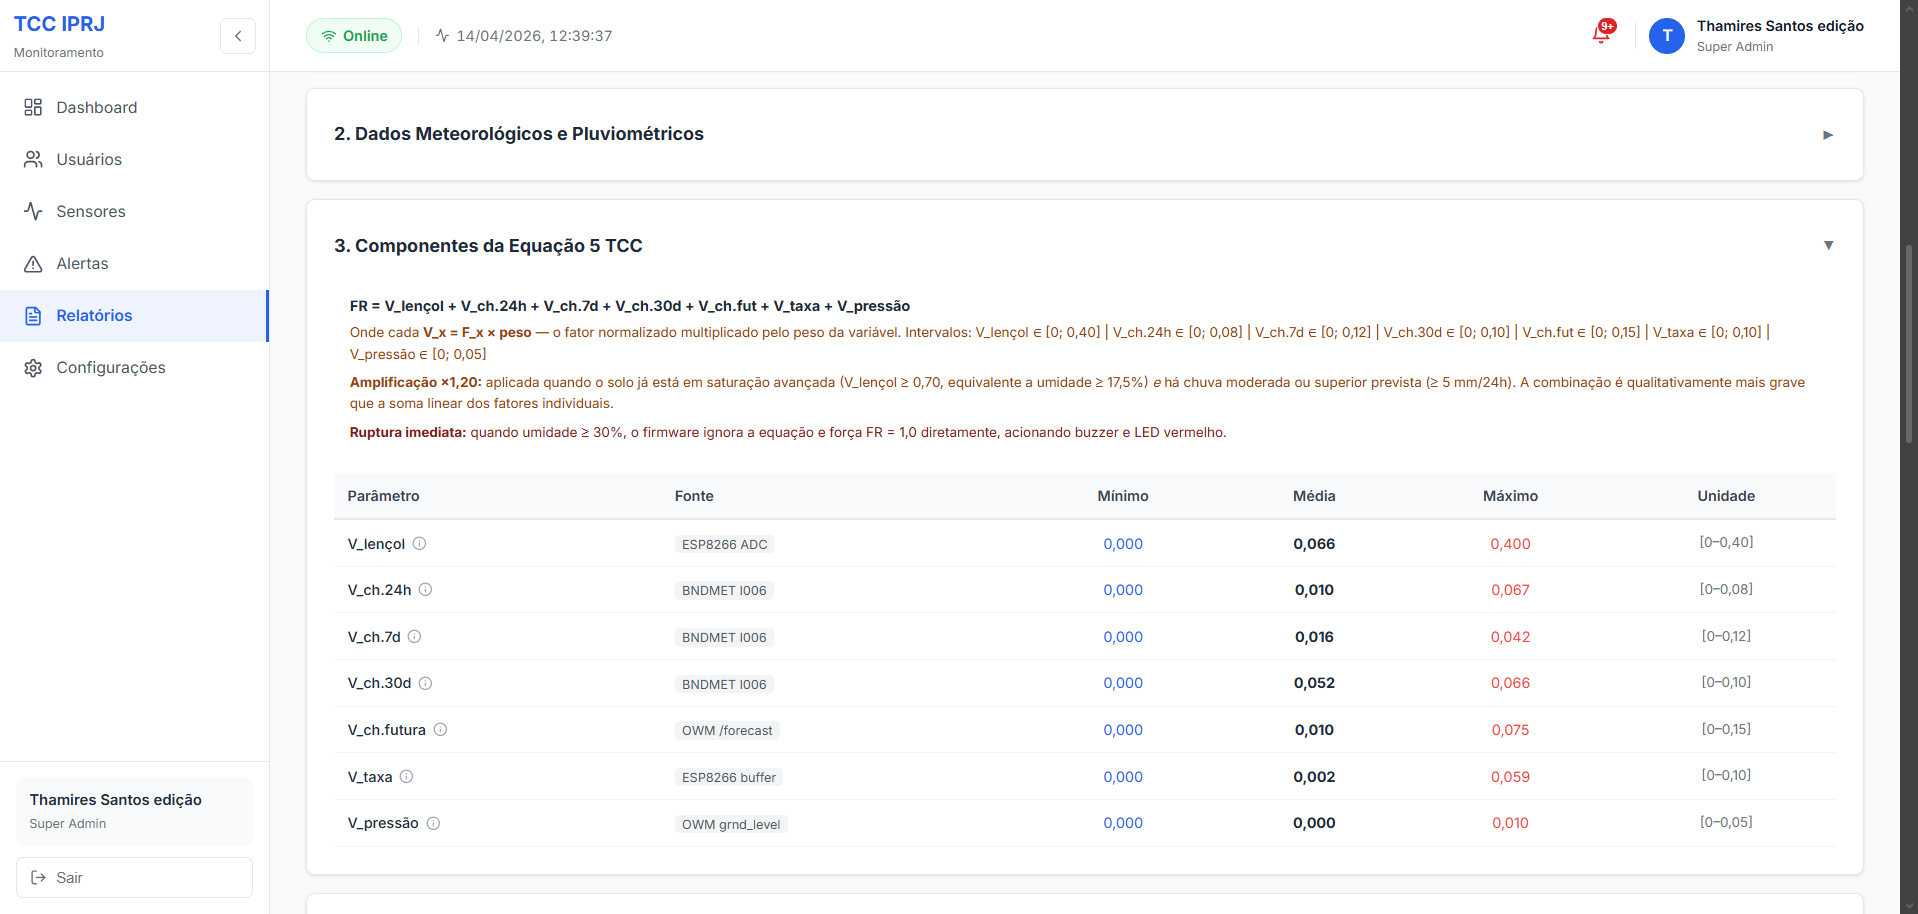
\includegraphics[width=0.95\textwidth]{figures/cap5_relatorio_gerado_pt3.png}
    \caption{Tela de Relatórios com relatório gerado (parte~3): seção
    Componentes da Equação~5 TCC com fórmula do fator de risco integrado,
    regras de amplificação e ruptura, e estatísticas dos sete componentes
    individuais do modelo.}
    \label{fig:relatorio_gerado_pt3}
    \fonte{Elaborado pela autora.}
\end{figure}

\begin{figure}[htbp]
    \centering
    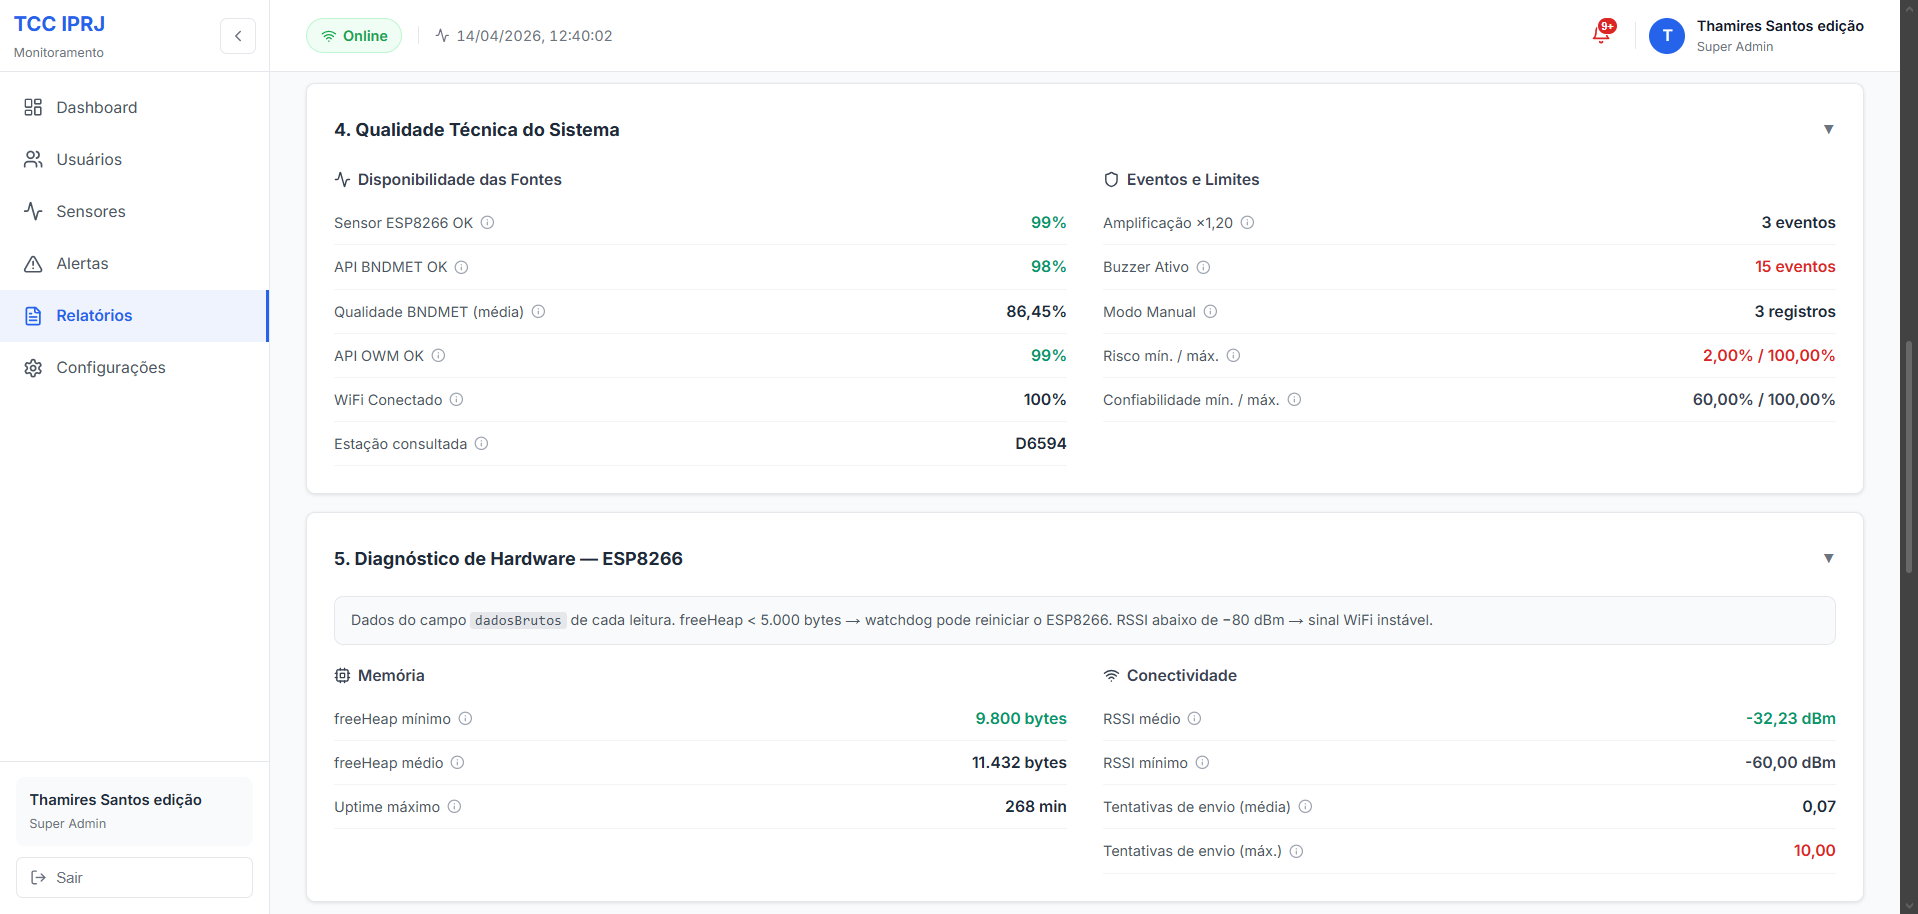
\includegraphics[width=0.95\textwidth]{figures/cap5_relatorio_gerado_pt4.png}
    \caption{Tela de Relatórios com relatório gerado (parte~4): seção
    Qualidade Técnica do Sistema com disponibilidade das fontes e eventos
    e limites do período, e seção Diagnóstico de Hardware ESP8266 com
    estatísticas de memória e conectividade.}
    \label{fig:relatorio_gerado_pt4}
    \fonte{Elaborado pela autora.}
\end{figure}

\begin{figure}[htbp]
    \centering
    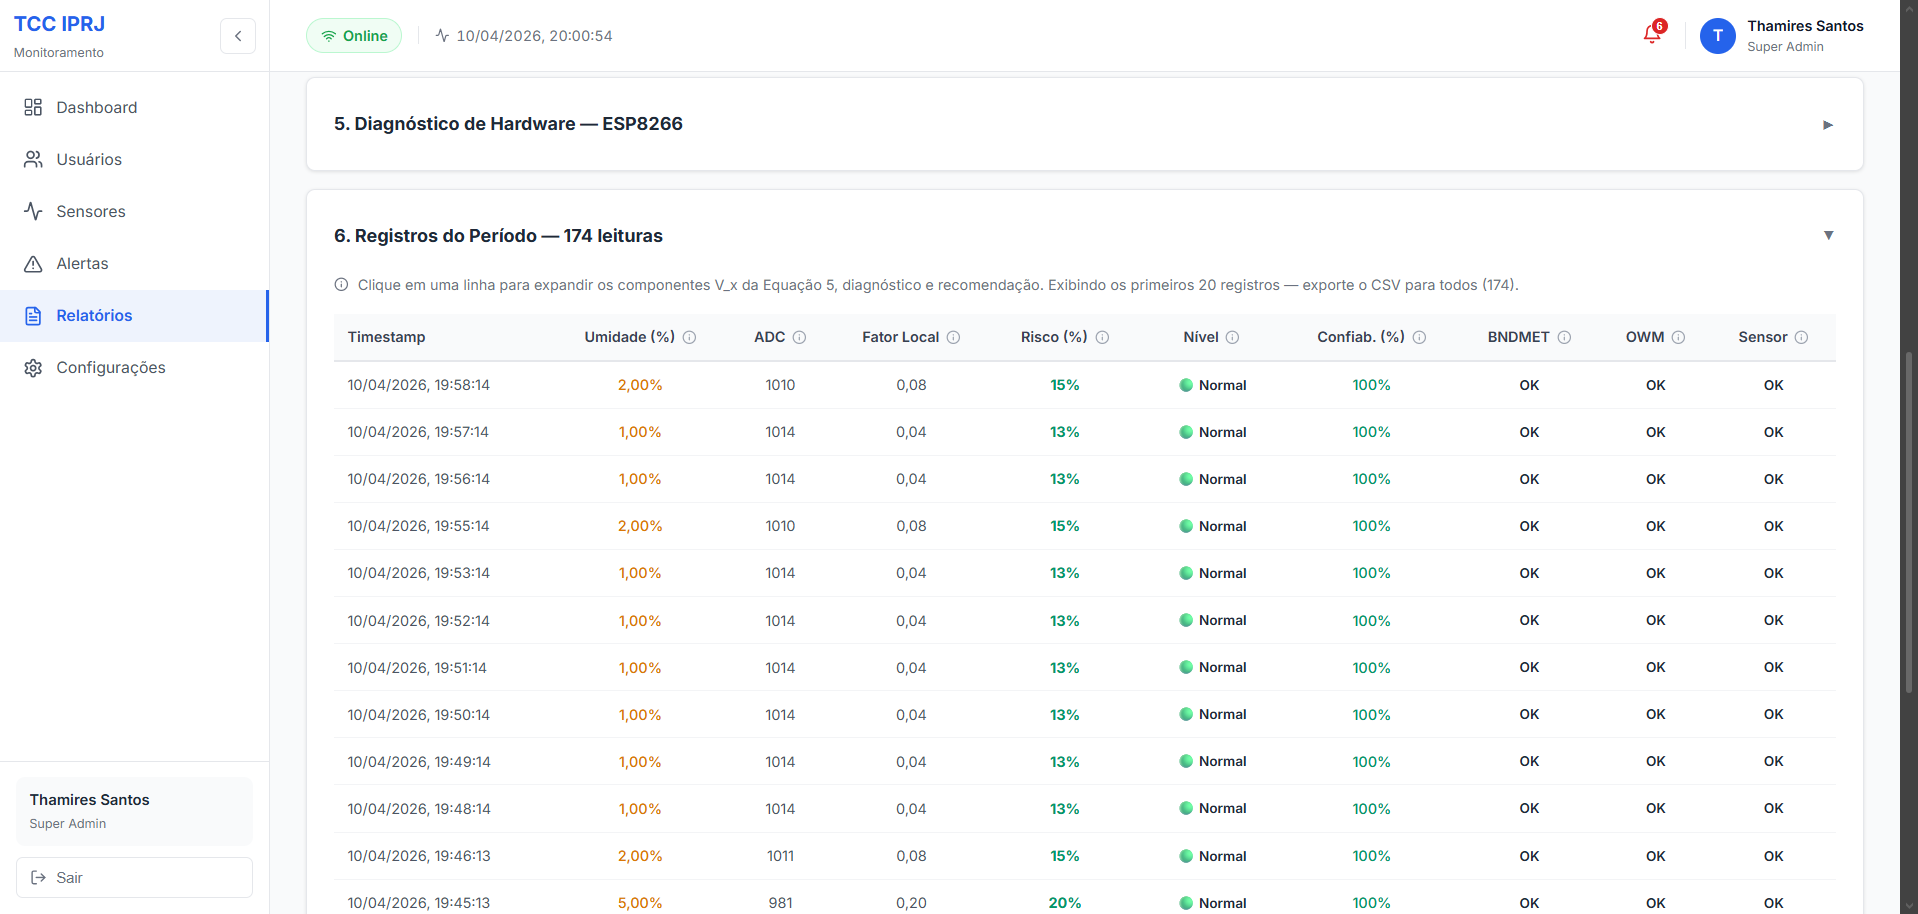
\includegraphics[width=0.95\textwidth]{figures/cap5_relatorio_gerado_pt5.png}
    \caption{Tela de Relatórios com relatório gerado (parte~5): seção
    Registros do Período com tabela paginada exibindo os primeiros
    registros --- \textit{timestamp}, umidade, ADC, risco, nível,
    confiabilidade e \textit{status} das fontes.}
    \label{fig:relatorio_gerado_pt5}
    \fonte{Elaborado pela autora.}
\end{figure}

\begin{figure}[htbp]
    \centering
    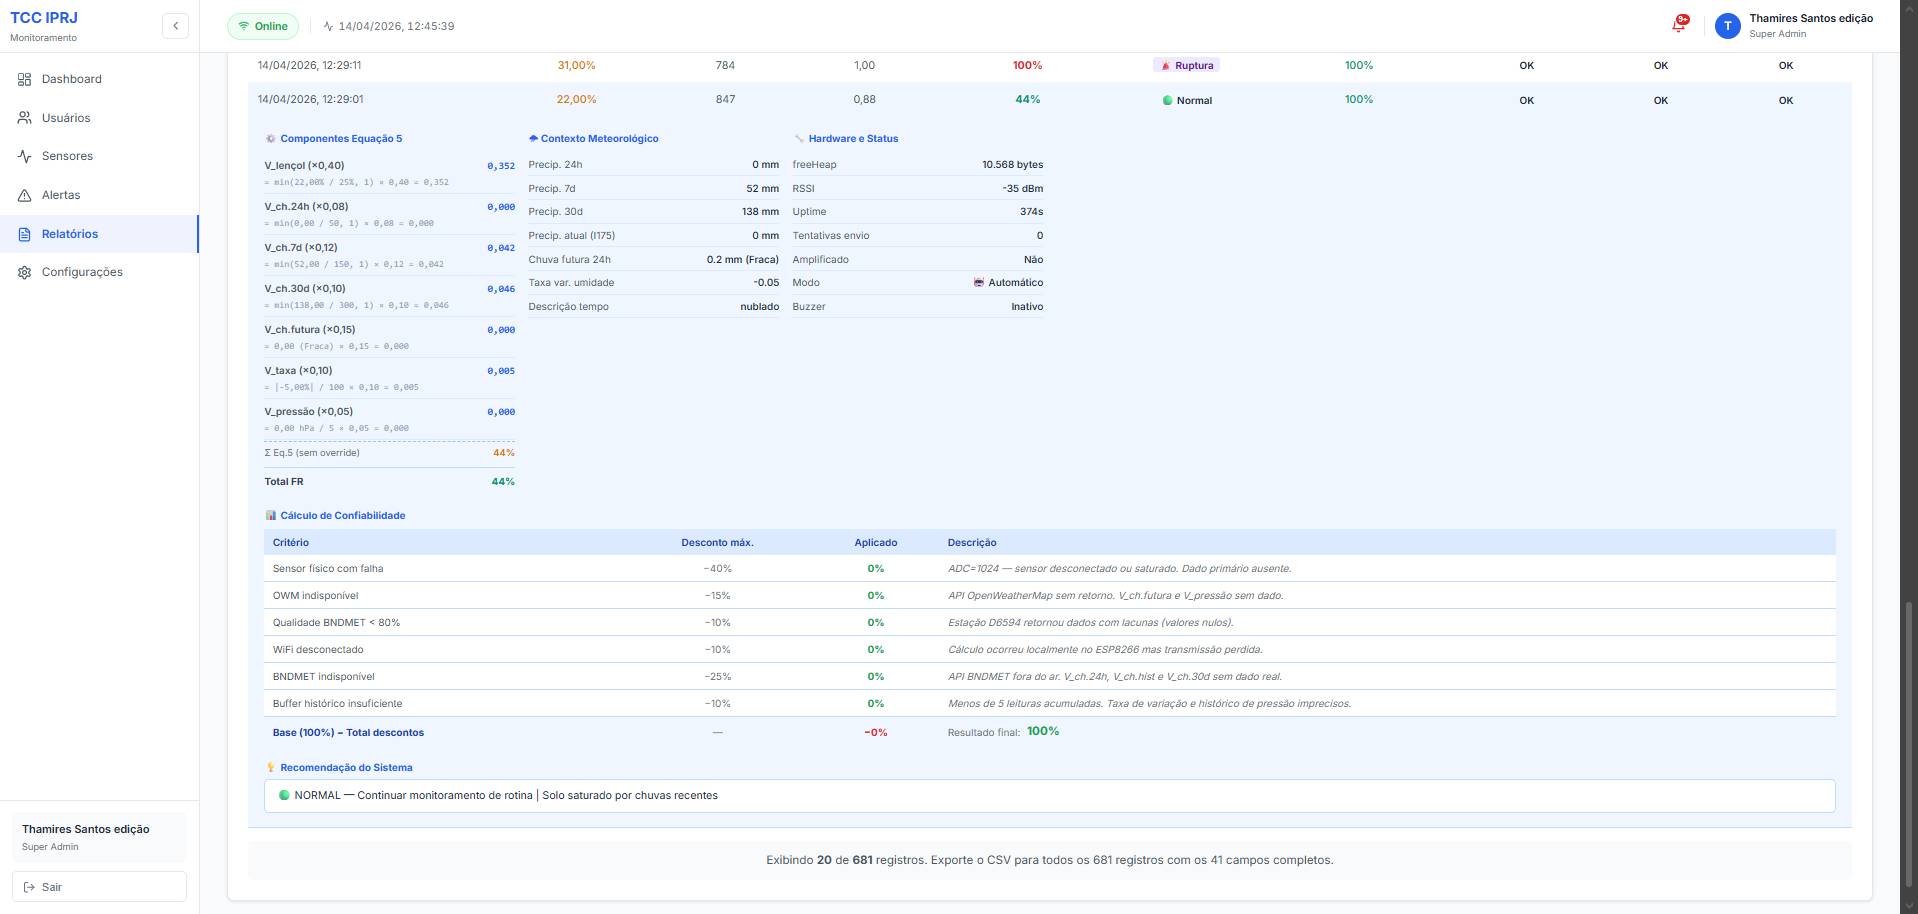
\includegraphics[width=0.95\textwidth]{figures/cap5_relatorio_gerado_pt6.png}
    \caption{Tela de Relatórios com relatório gerado (parte~6): continuação
    da tabela de registros e rodapé informando o total de leituras no
    período, com recomendação de exportação CSV para acesso aos 41~campos
    completos.}
    \label{fig:relatorio_gerado_pt6}
    \fonte{Elaborado pela autora.}
\end{figure}

Quando as datas não são informadas, ao clicar em ``Gerar Relatório'',
o sistema exibe o \textit{toast} ``Selecione as datas de início e fim'', conforme ilustra a \autoref{fig:relatorio_erros_validacao_pt_1}.
Falhas de comunicação com o \textit{backend} exibem o \textit{toast} ``Erro
ao gerar relatório. Verifique se o servidor está acessível'' e mantêm o relatório com os campos zerados em tela, conforme
ilustra a \autoref{fig:relatorio_erros_validacao_pt_2}. Quando há
dados no período mas as estatísticas resultam em valores zerados por não
haver leituras em alguma janela específica, o \textit{toast} ``Nenhum dado
encontrado para o período selecionado'' é exibido e as seções são apresentadas com os zeros
correspondentes, conforme ilustra a \autoref{fig:relatorio_erros_validacao_pt_3}.

\begin{figure}[htbp]
    \centering
    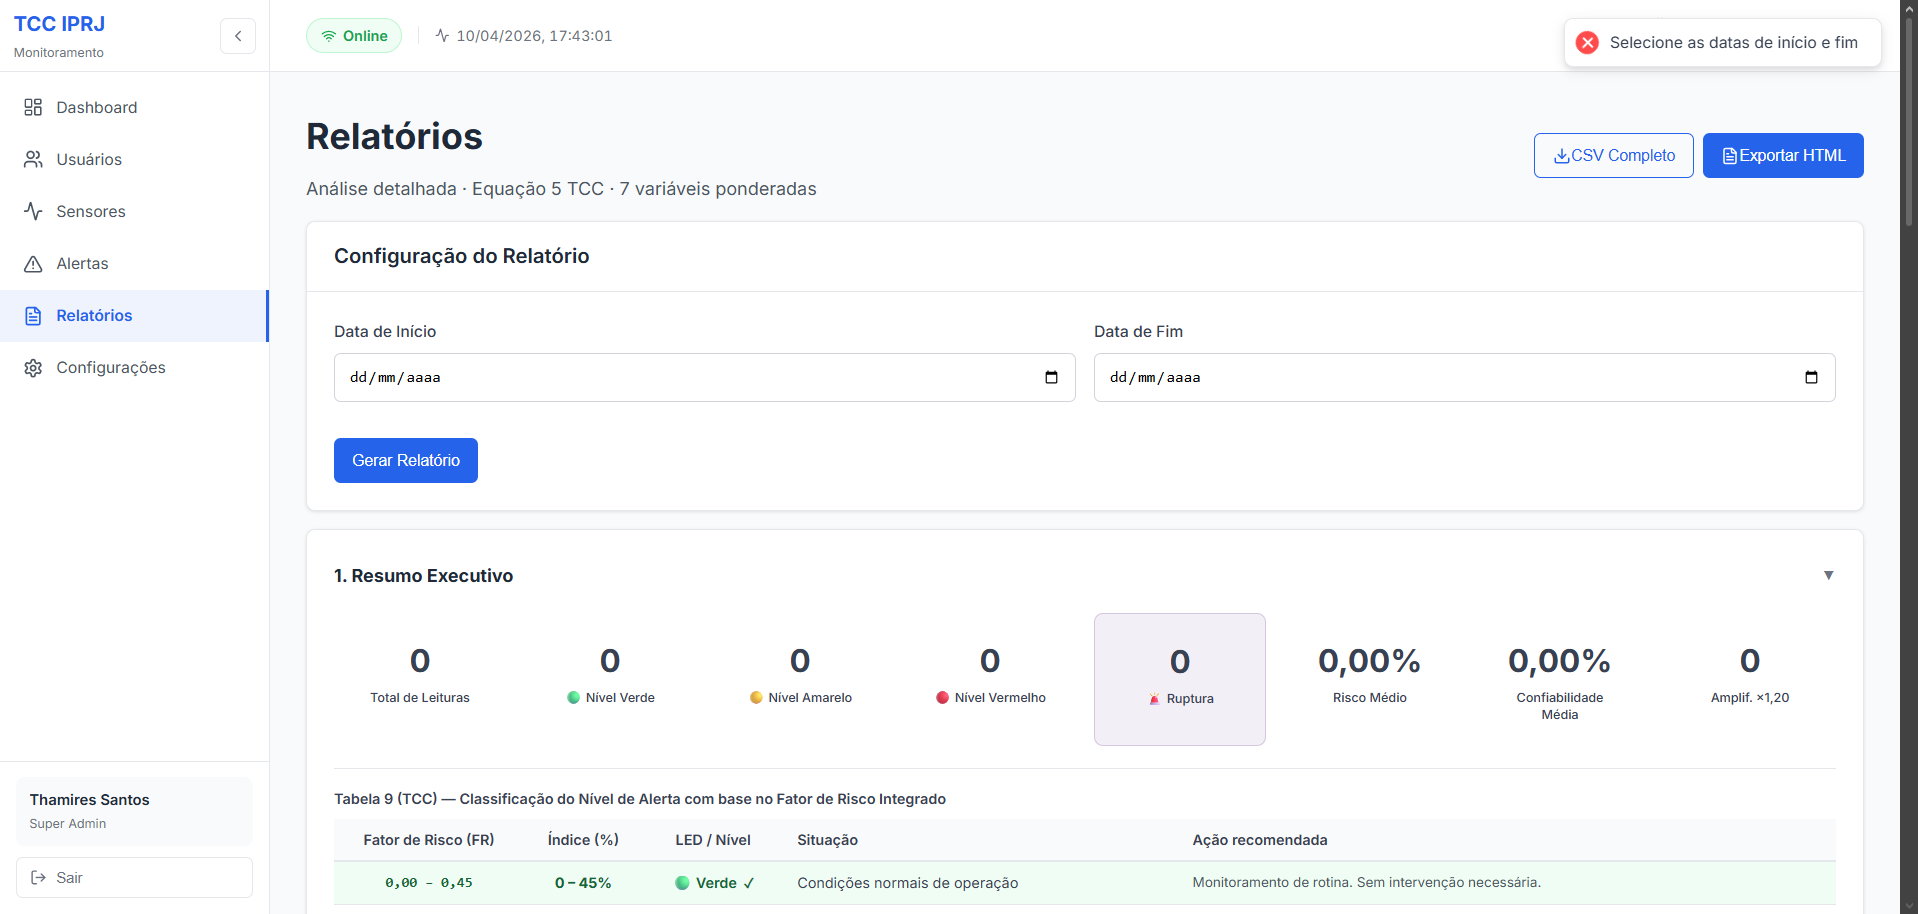
\includegraphics[width=0.95\textwidth]{figures/cap5_relatorio_erros_validacao_pt1.png}
    \caption{Tela de Relatórios com cenários de erro: \textit{toast} ``Selecione as datas de início e fim'' por datas não informadas.}
    \label{fig:relatorio_erros_validacao_pt_1}
    \fonte{Elaborado pela autora.}
\end{figure}

\begin{figure}[htbp]
    \centering
    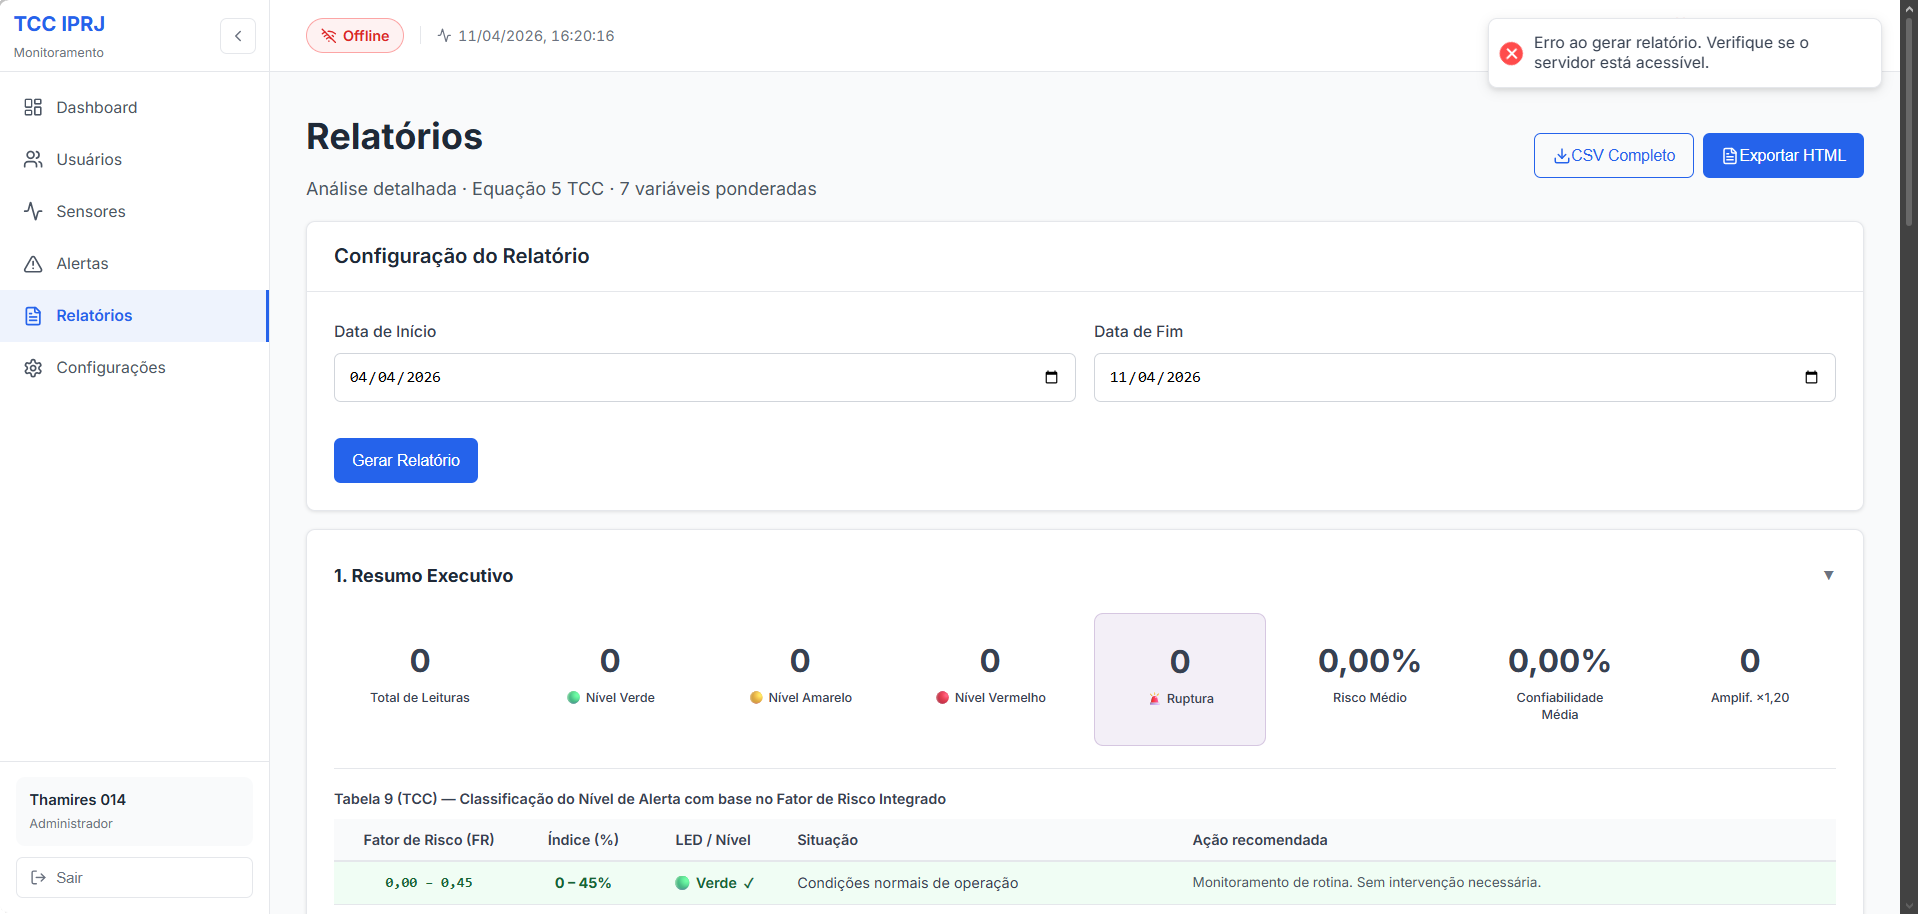
\includegraphics[width=0.95\textwidth]{figures/cap5_relatorio_erros_validacao_pt2.png}
    \caption{Tela de Relatórios com cenários de erro: \textit{toast} ``Erro ao gerar relatório. Verifique se o servidor está acessível'' por falha de comunicação.}
    \label{fig:relatorio_erros_validacao_pt_2}
    \fonte{Elaborado pela autora.}
\end{figure}

\begin{figure}[htbp]
    \centering
    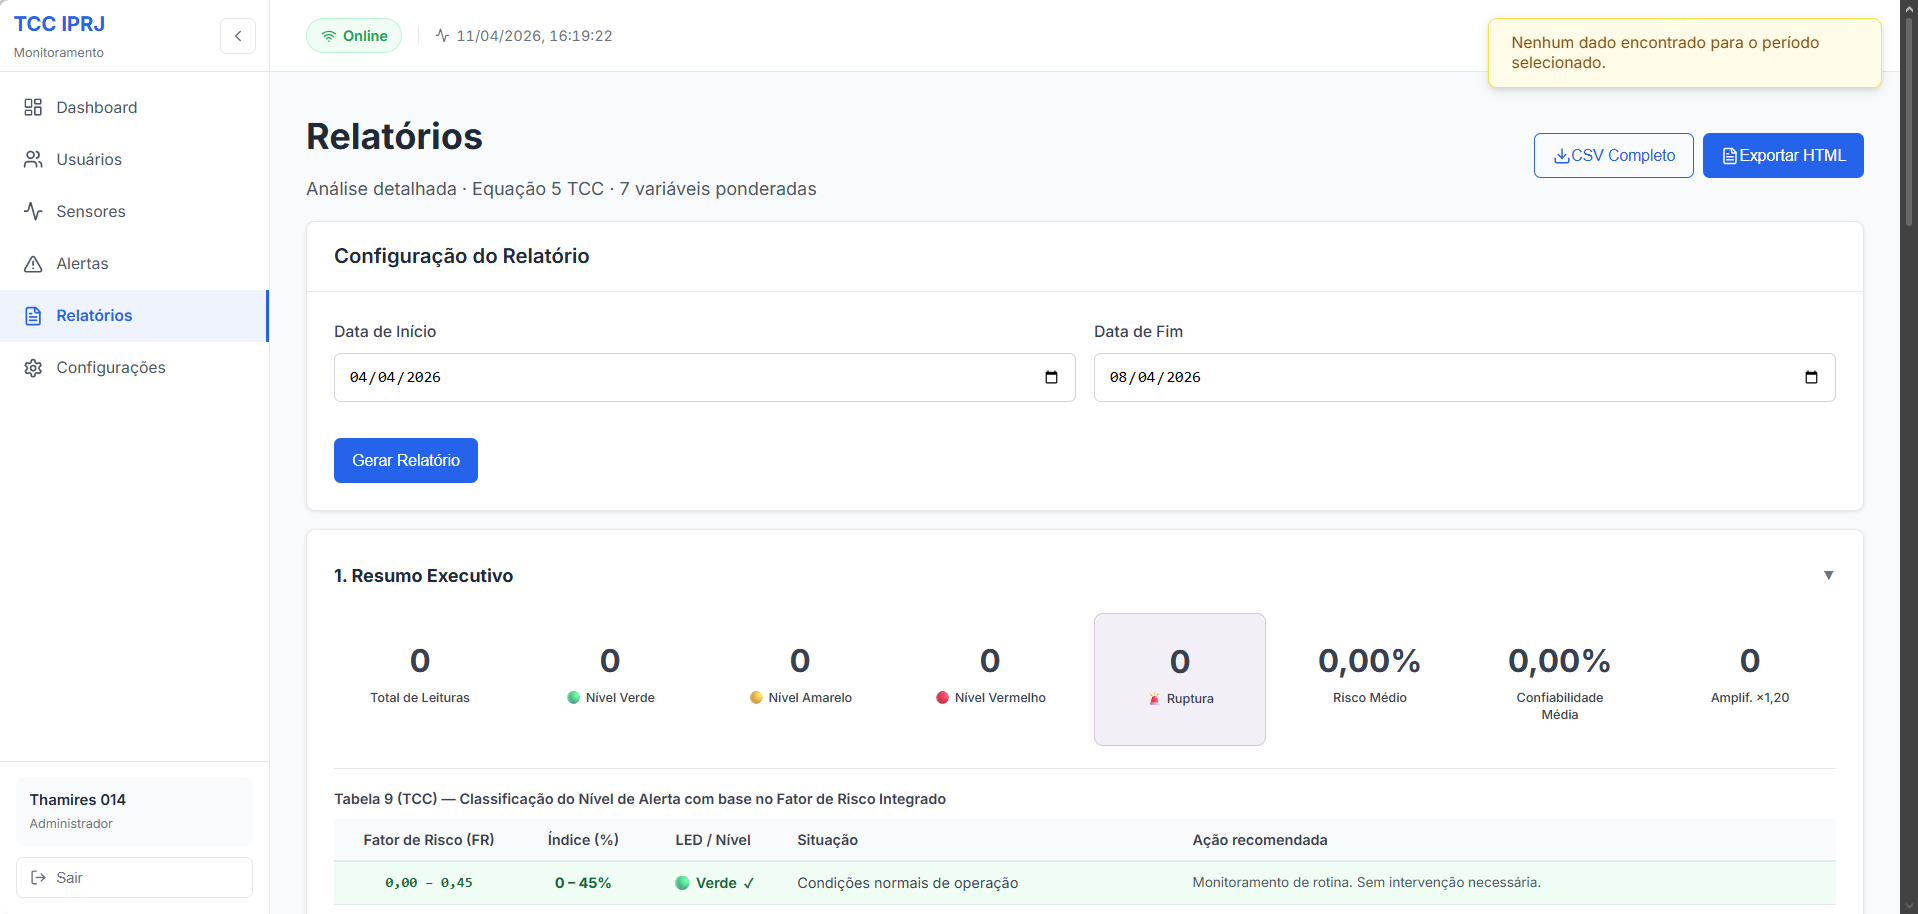
\includegraphics[width=0.95\textwidth]{figures/cap5_relatorio_erros_validacao_pt3.png}
    \caption{Tela de Relatórios com cenários de erro: \textit{toast} ``Nenhum dado encontrado para o período selecionado'' por período sem leituras.}
    \label{fig:relatorio_erros_validacao_pt_3}
    \fonte{Elaborado pela autora.}
\end{figure}

% -------------------------------------------------------------
\subsection{Exportação em CSV}
\label{subsec:relatorio-csv}
% -------------------------------------------------------------

O botão ``CSV Completo'' gera um arquivo com BOM UTF-8 e 41 colunas,
nomeado com as datas de início e fim do período analisado no formato
\texttt{relatorio\_AAAA-MM-DD\_AAAA-MM-DD.csv}. Ao concluir, o
\textit{toast} ``CSV exportado com sucesso!'' confirma o \textit{download}, conforme mostra a \autoref{fig:relatorio_csv_sucesso}.
Quando o relatório não contém dados, o \textit{toast} ``Nenhum dado para
exportar'' é exibido e nenhum arquivo é gerado, conforme ilustra a \autoref{fig:relatorio_csv_sem_dados}.

\begin{figure}[htbp]
    \centering
    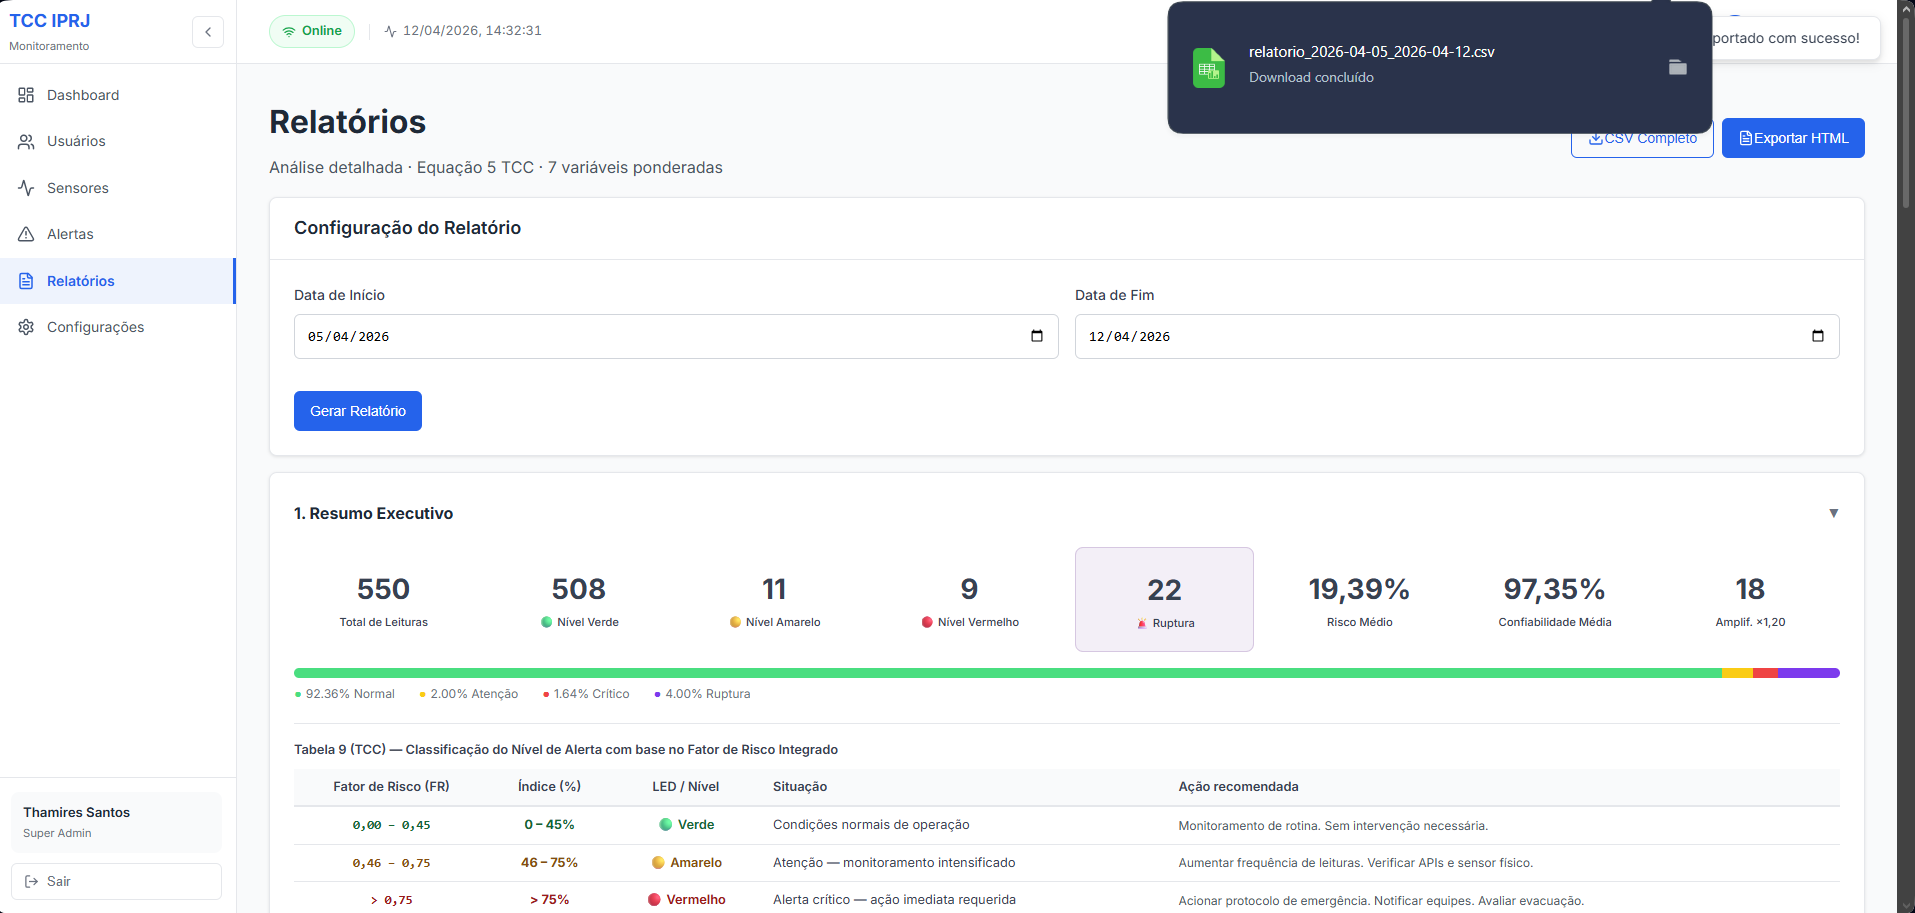
\includegraphics[width=0.95\textwidth]{figures/cap5_relatorio_csv_sucesso.png}
    \caption{Tela de Relatórios com \textit{toast} ``CSV exportado com sucesso!'' e o arquivo baixado, ao gerar CSV de relatório com leituras no período selecionado.}
    \label{fig:relatorio_csv_sucesso}
    \fonte{Elaborado pela autora.}
\end{figure}

\begin{figure}[htbp]
    \centering
    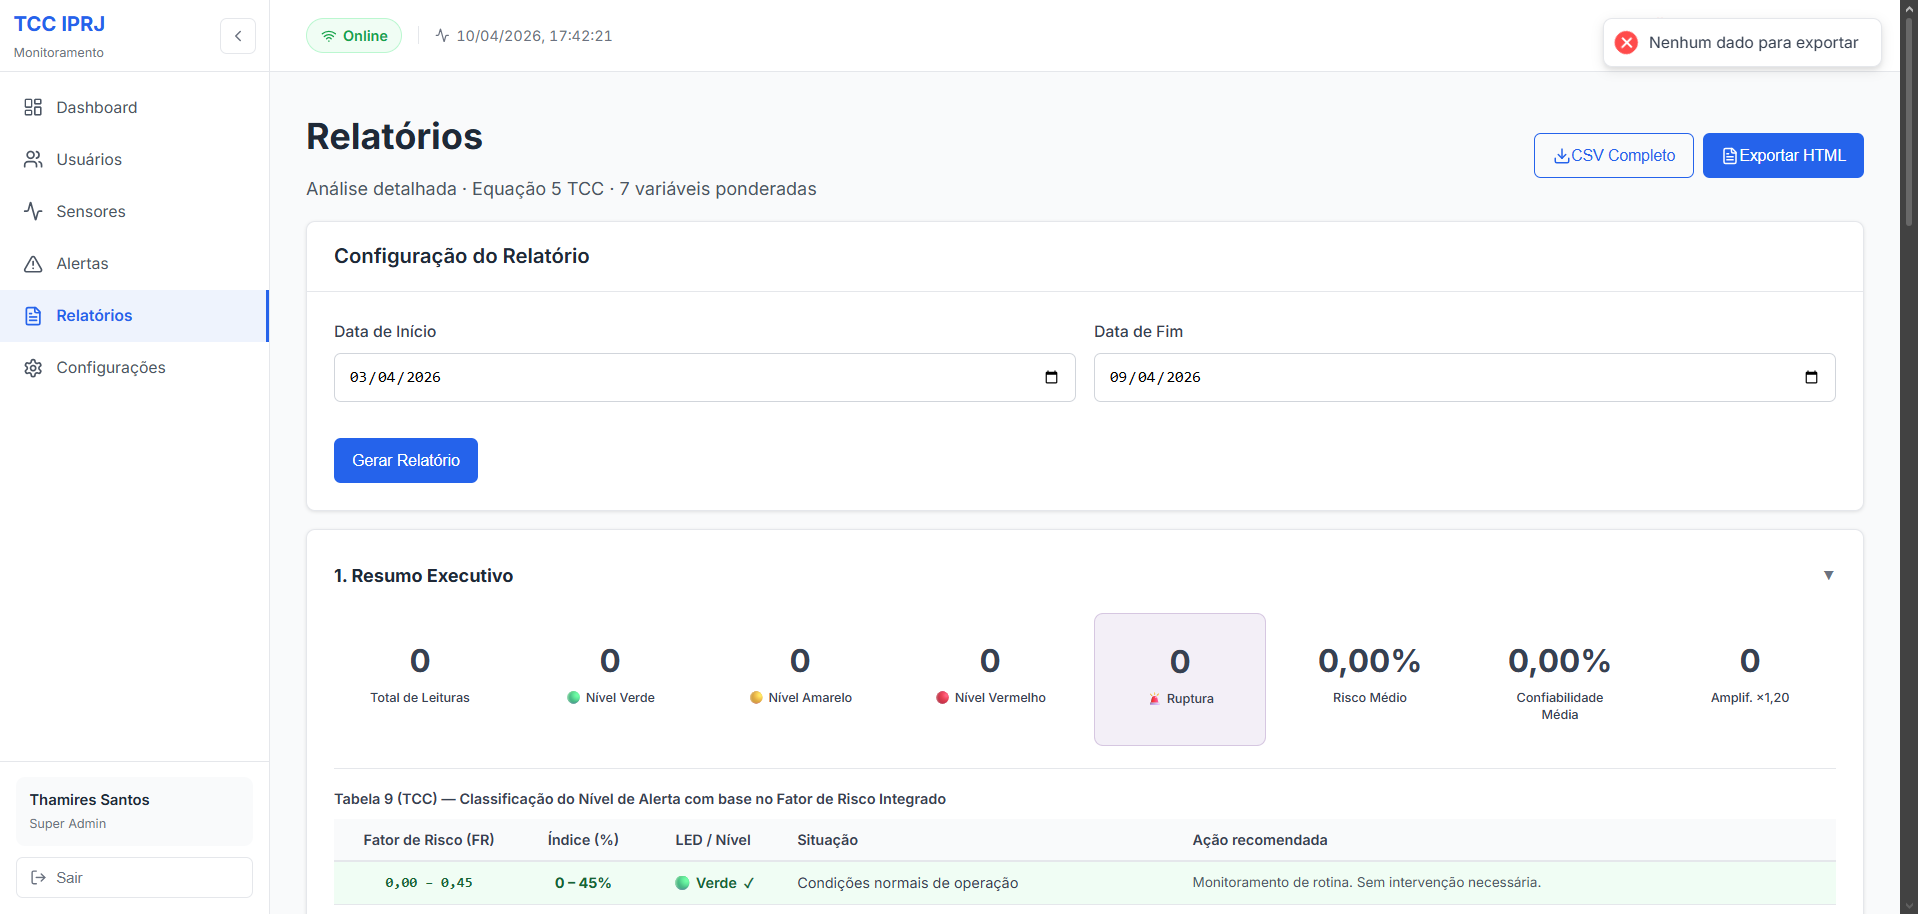
\includegraphics[width=0.95\textwidth]{figures/cap5_relatorio_csv_sem_dados.png}
    \caption{Tela de Relatórios com \textit{toast} ``Nenhum dado para exportar'' ao tentar gerar CSV de relatório sem leituras no período selecionado.}
    \label{fig:relatorio_csv_sem_dados}
    \fonte{Elaborado pela autora.}
\end{figure}

% -------------------------------------------------------------
\subsection{Exportação em HTML}
\label{subsec:relatorio-html}
% -------------------------------------------------------------

O botão ``Exportar HTML'' gera um relatório completo com todos os estilos
\textit{inline}, que pode ser aberto em qualquer navegador sem dependências
externas, arquivado ou enviado por e-mail como anexo. As
\autoref{fig:relatorio_html_pt1}, \autoref{fig:relatorio_html_pt2} e
\autoref{fig:relatorio_html_pt3} exibem o arquivo aberto no navegador com a
mesma estrutura das seis seções, formatação de tabelas e barra de
distribuição por nível de alerta. Após clicar no botão ``Exportar HTML'', o \textit{toast} ``Relatório HTML
exportado!'' confirma o \textit{download}, em que o arquivo é nomeado com as datas de início e fim do período analisado no formato
\texttt{relatorio\_AAAA-MM-DD\_AAAA-MM-DD.html}
conforme ilustra a \autoref{fig:relatorio_html_sucesso}.

\begin{figure}[htbp]
    \centering
    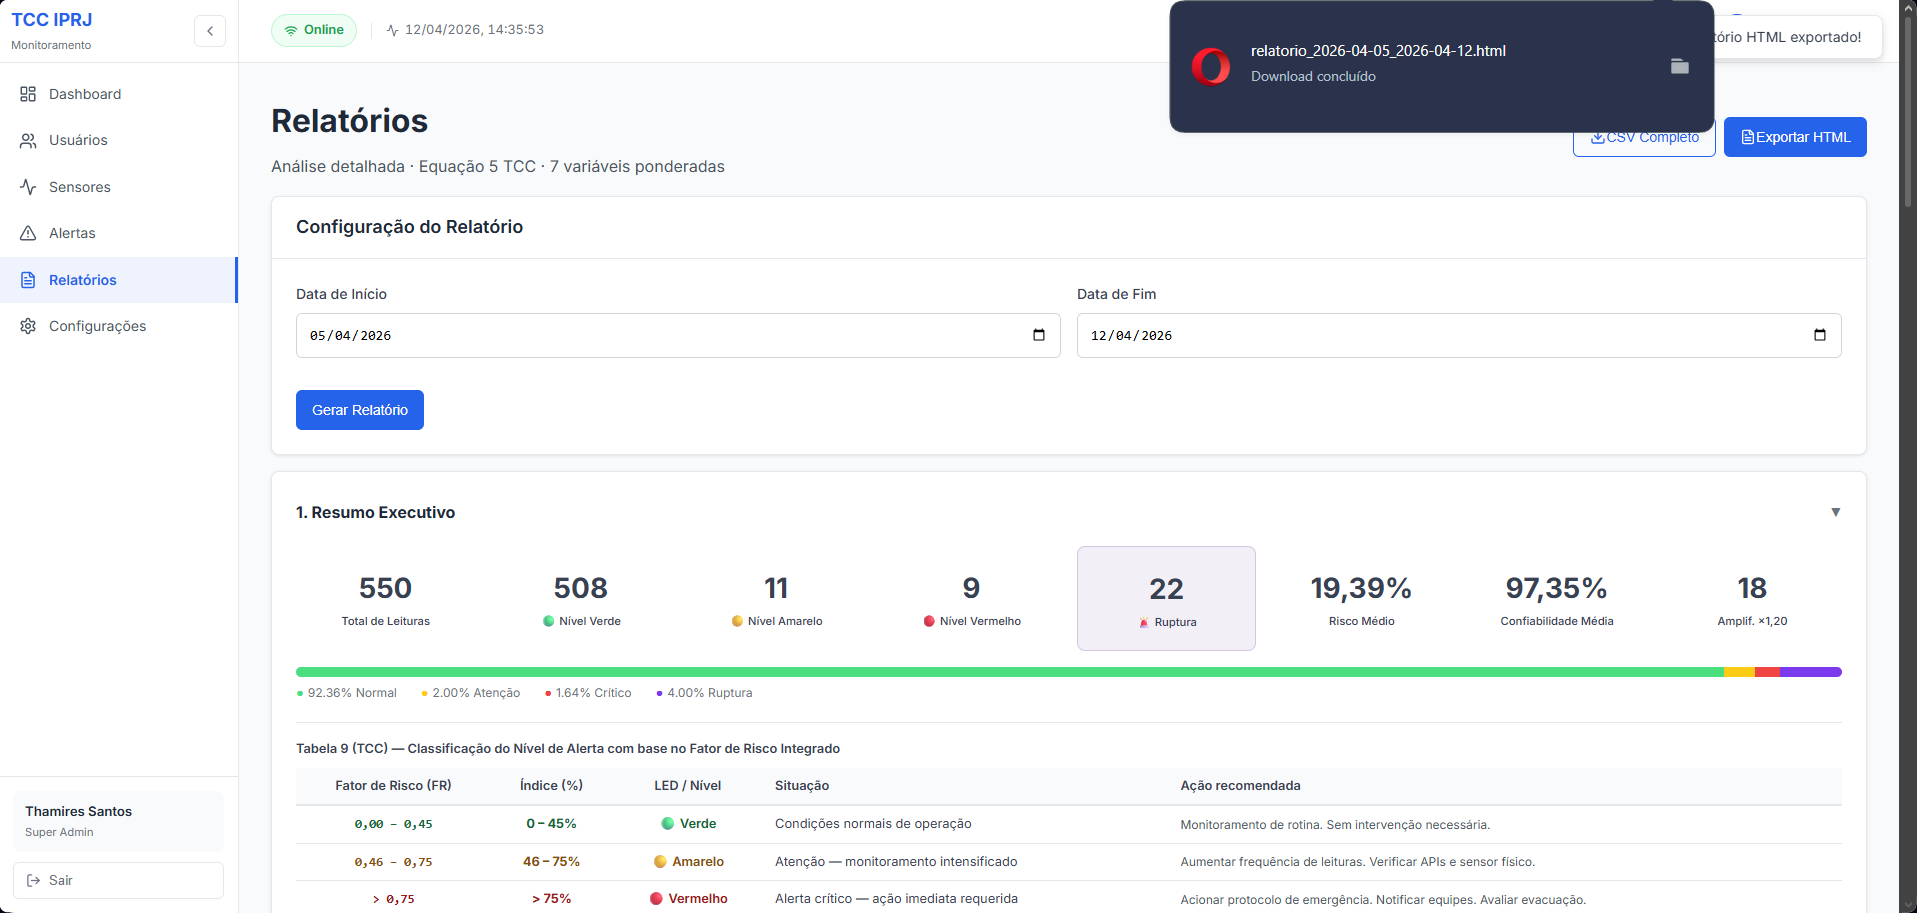
\includegraphics[width=0.95\textwidth]{figures/cap5_relatorio_html_sucesso.png}
    \caption{Tela de Relatórios com \textit{toast} ``Relatório HTML exportado!'' e o arquivo baixado, ao gerar HTML de relatório com leituras no período selecionado.}
    \label{fig:relatorio_html_sucesso}
    \fonte{Elaborado pela autora.}
\end{figure}

\begin{figure}[htbp]
    \centering
    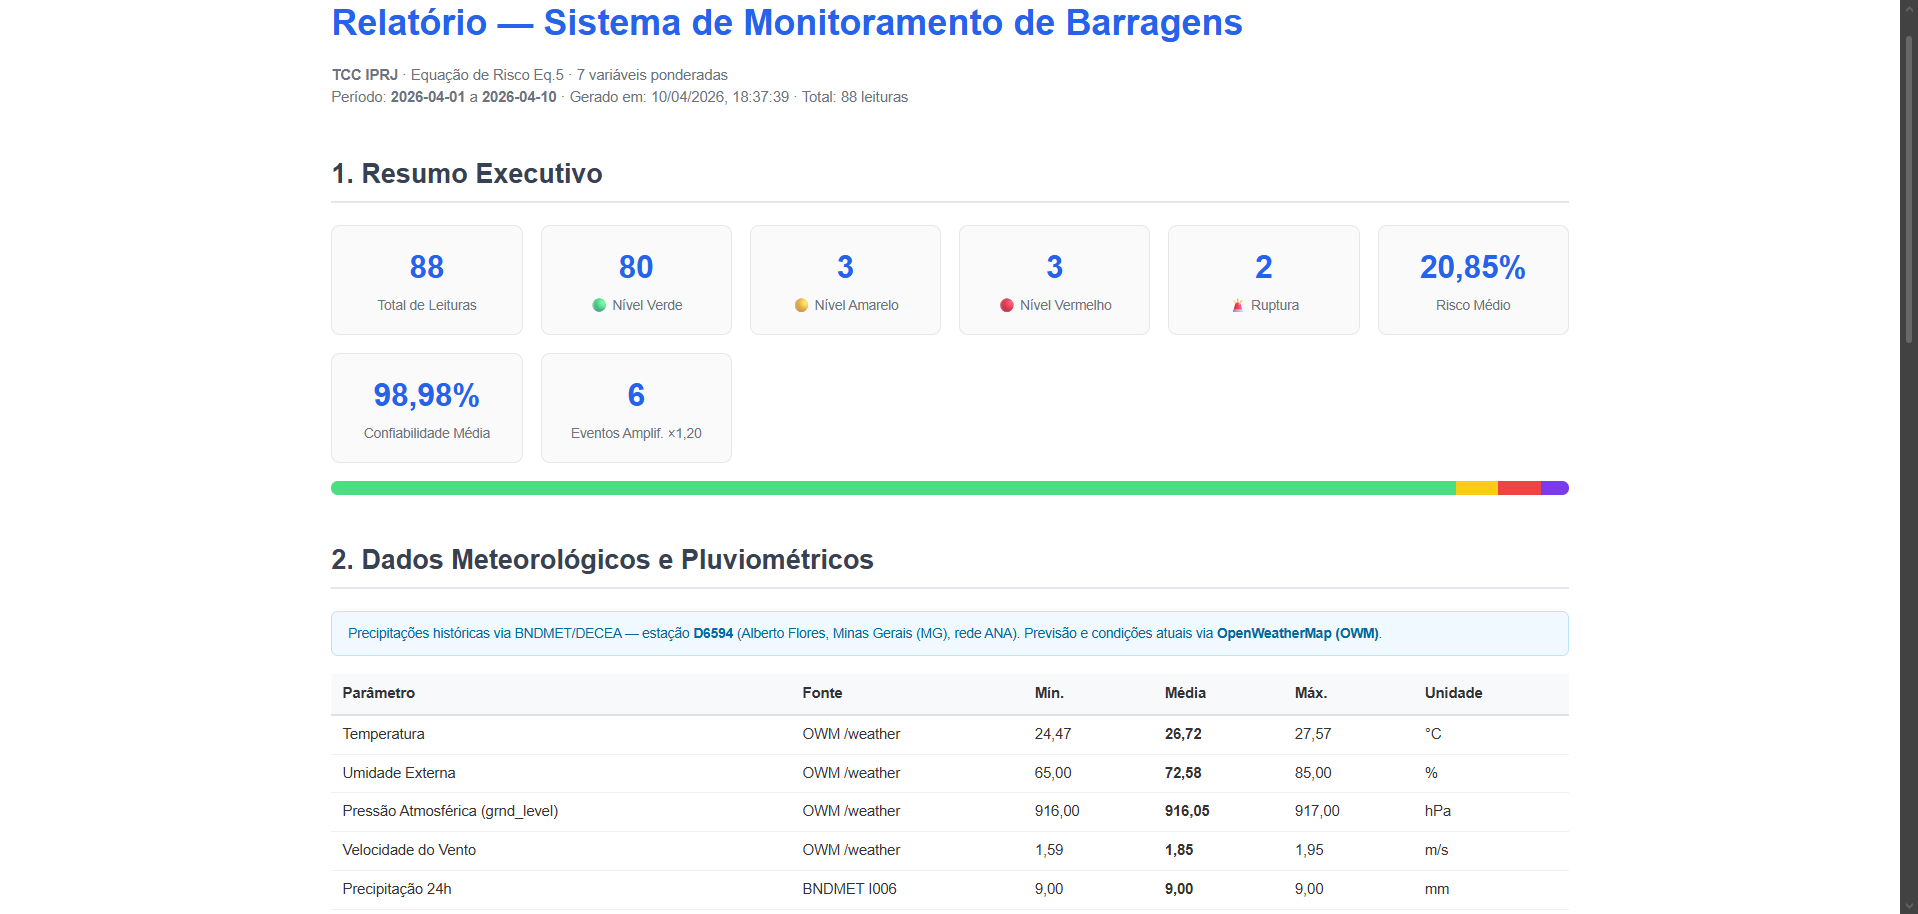
\includegraphics[width=0.95\textwidth]{figures/cap5_relatorio_html_pt1.png}
    \caption{Relatório HTML exportado aberto no navegador (parte~1):
    cabeçalho do documento, seção Resumo Executivo com barra de
    distribuição por nível de alerta e início da seção de dados meteorológicos.}
    \label{fig:relatorio_html_pt1}
    \fonte{Elaborado pela autora.}
\end{figure}

\begin{figure}[htbp]
    \centering
    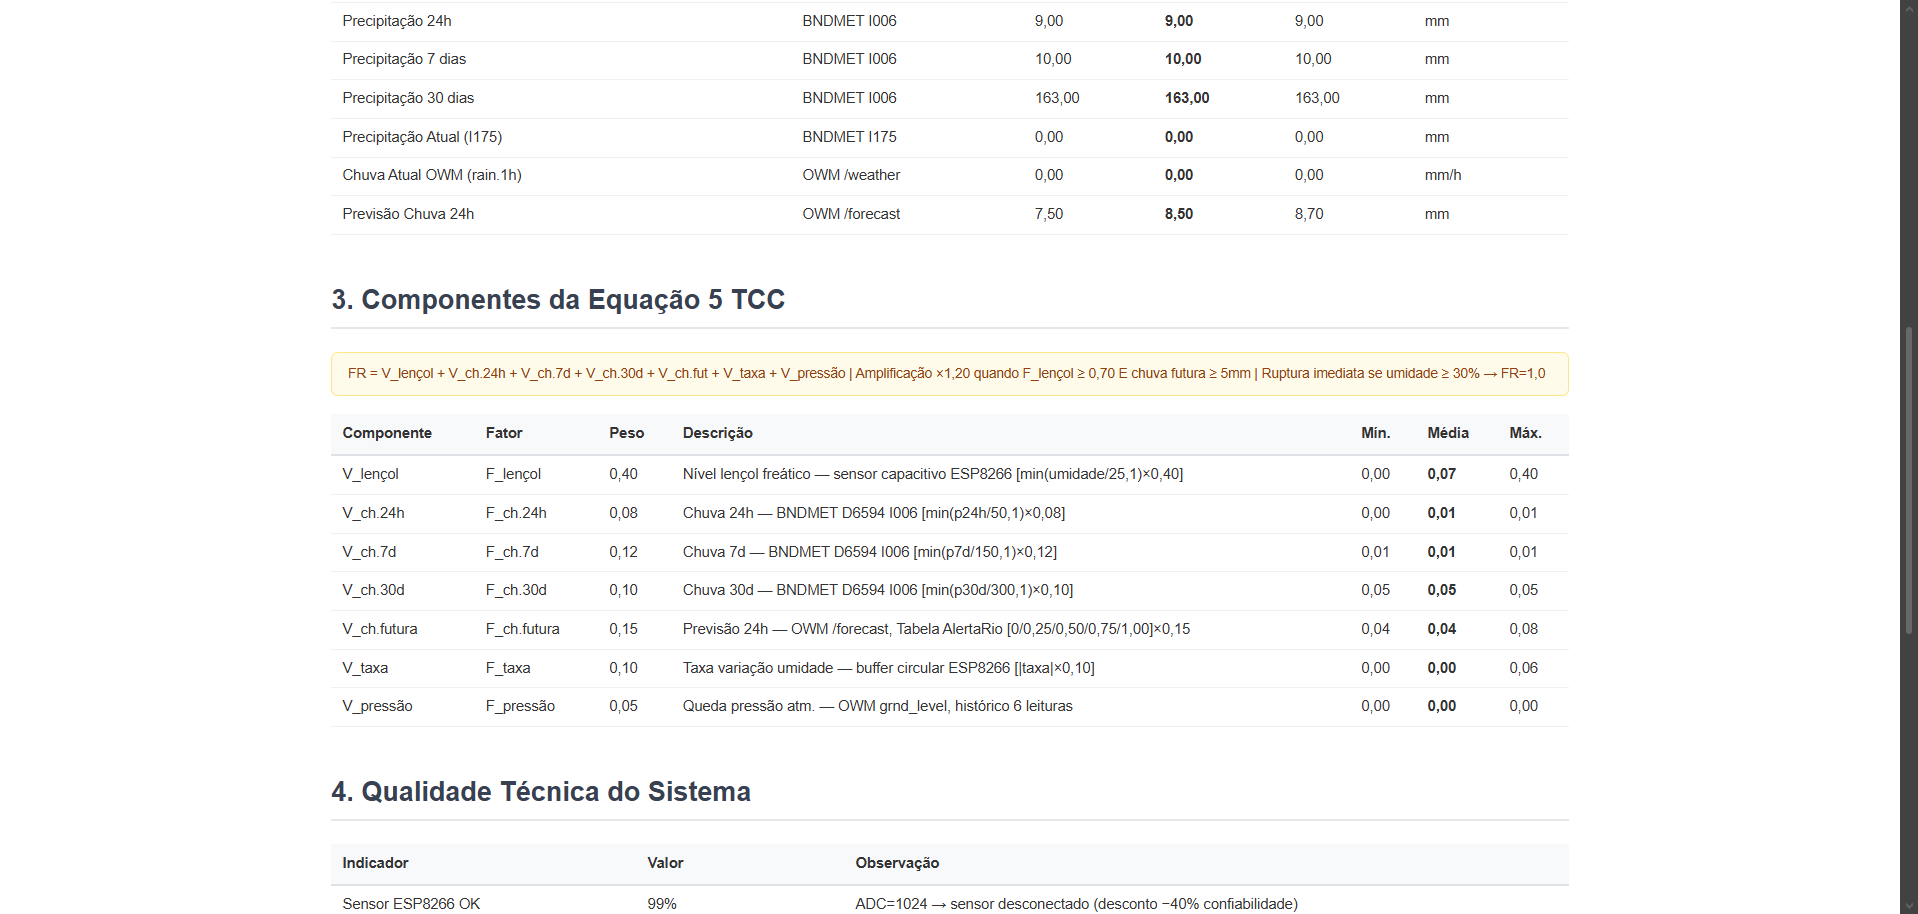
\includegraphics[width=0.95\textwidth]{figures/cap5_relatorio_html_pt2.png}
    \caption{Relatório HTML exportado aberto no navegador (parte~2):
    continuação da seção de dados meteorológicos e componentes do modelo de risco
    com tabelas estatísticas.}
    \label{fig:relatorio_html_pt2}
    \fonte{Elaborado pela autora.}
\end{figure}

\begin{figure}[htbp]
    \centering
    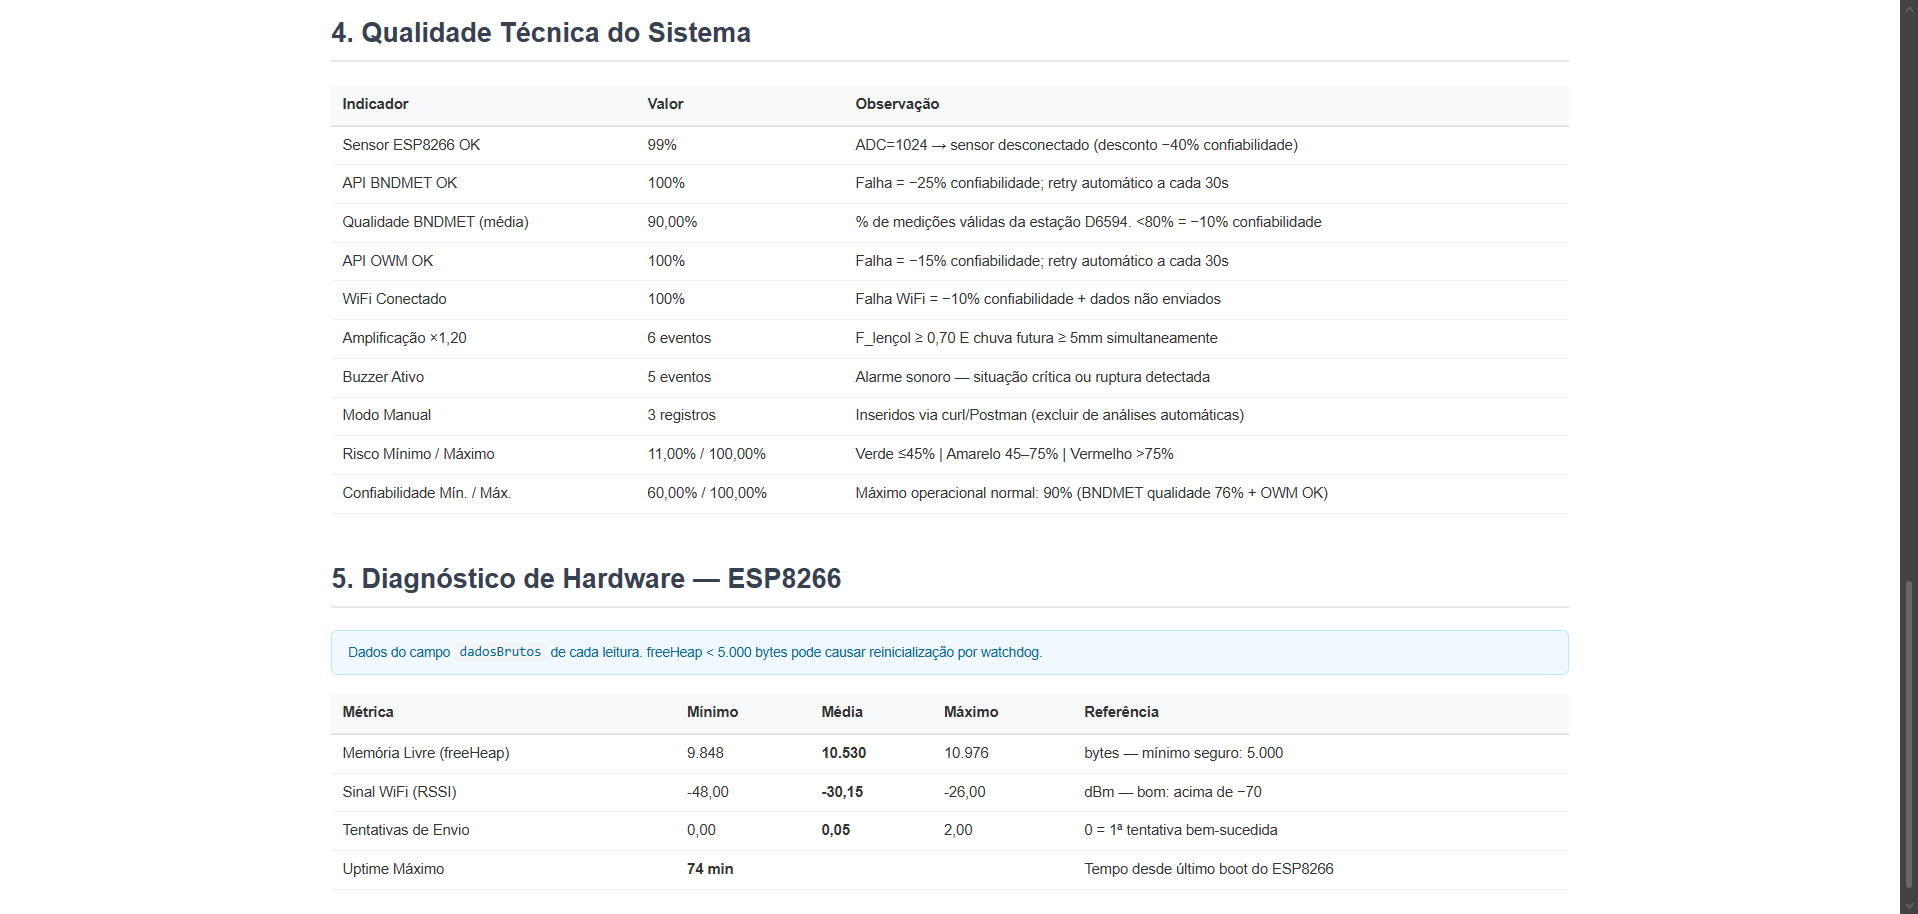
\includegraphics[width=0.95\textwidth]{figures/cap5_relatorio_html_pt3.png}
    \caption{Relatório HTML exportado aberto no navegador (parte~3):
    seções de qualidade técnica e diagnóstico de \textit{hardware}o.}
    \label{fig:relatorio_html_pt3}
    \fonte{Elaborado pela autora.}
\end{figure}

% =============================================================
\section{Gestão de Usuários e Administradores}
\label{sec:usuarios}
% =============================================================

% -------------------------------------------------------------
\subsection{Listagem, Abas e Filtro}
\label{subsec:usuarios-listagem}
% -------------------------------------------------------------

A tela de Gestão de Usuários organiza em duas abas o acesso aos dois
perfis do sistema. A aba ``Usuários Básicos'' está disponível para todos
os administradores; a aba ``Administradores'' é restrita ao perfil
\textit{super\_admin}. A \autoref{fig:usuarios_basicos} mostra a tela
com a aba de usuários básicos ativa: seis KPIs de contagem --- total de
usuários, admins ativos, básicos ativos, com notificações, inativos e
alertas enviados nos últimos 30 dias --- seguidos das abas de alternância,
um campo de busca por nome ou e-mail e a tabela paginada a 10 registros
por página.

\begin{figure}[htbp]
    \centering
    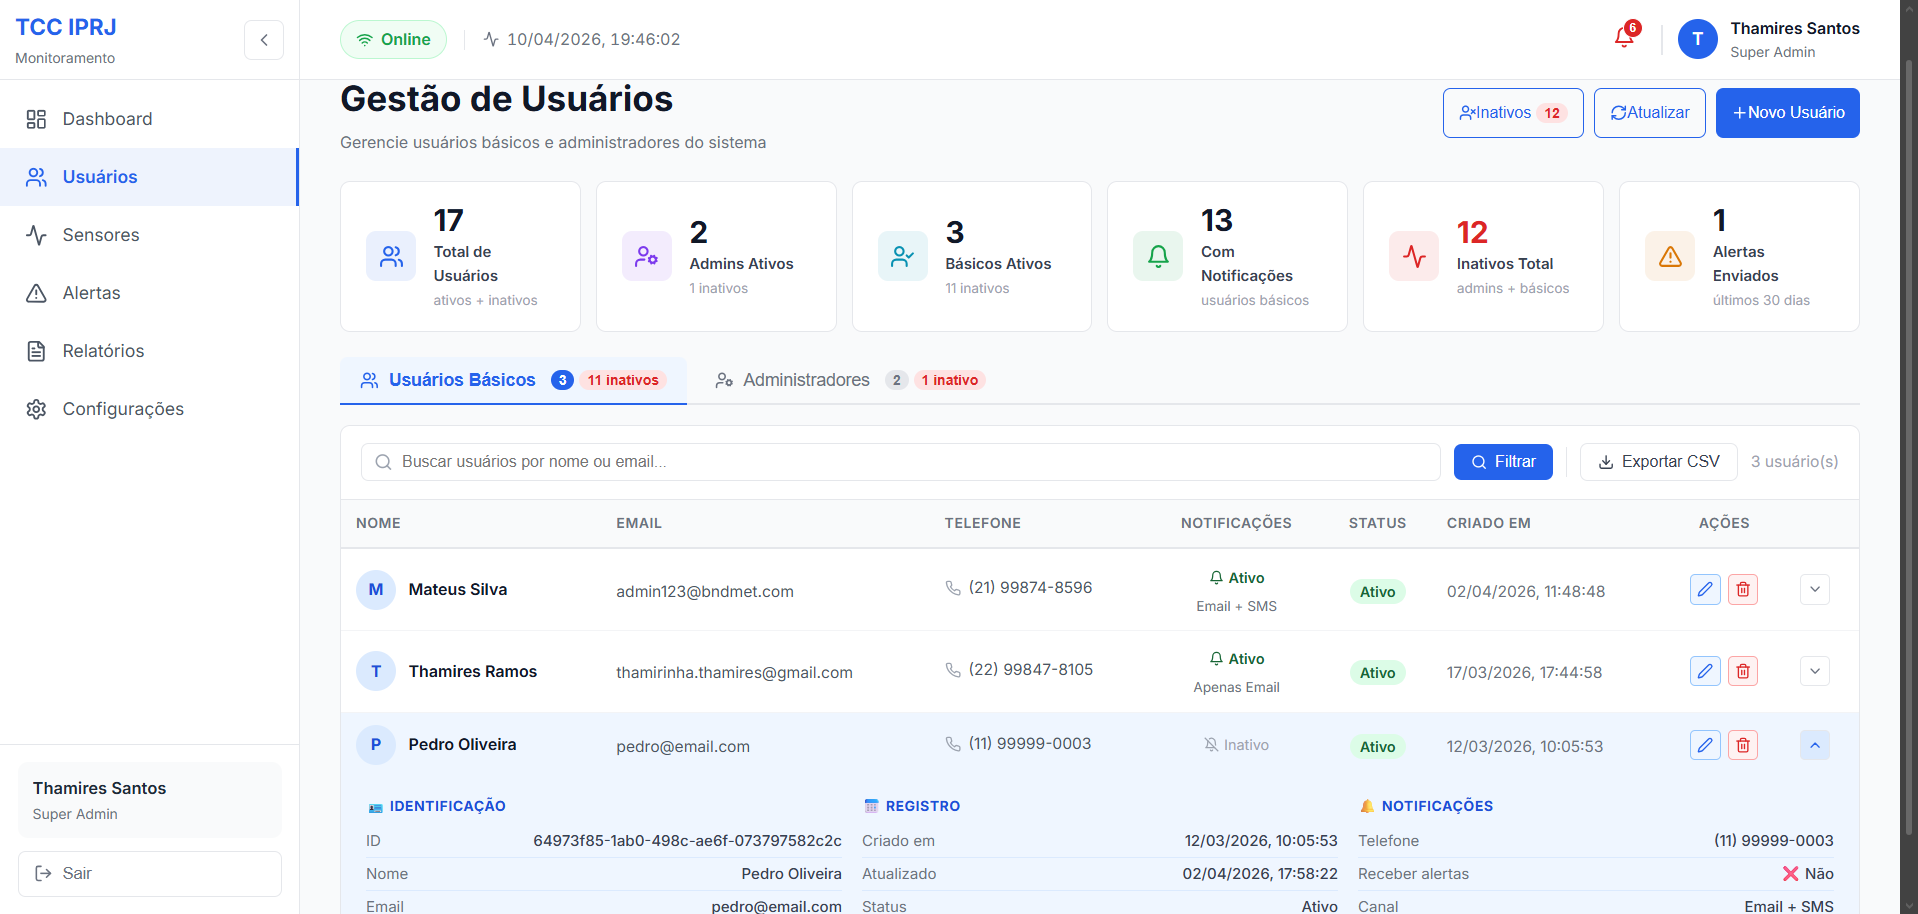
\includegraphics[width=0.95\textwidth]{figures/cap5_usuarios_basicos.png}
    \caption{Tela de Gestão de Usuários com aba ``Usuários Básicos'' ativa:
    KPIs de contagem, campo de busca e tabela paginada com ações por linha.}
    \label{fig:usuarios_basicos}
    \fonte{Elaborado pela autora.}
\end{figure}

Ao clicar em
\textbf{"Administradores"}, a lista é recarregada com os
registros de administradores, os filtros anteriores são limpos
e as opções de exportação refletem o novo contexto, conforme
ilustra a \autoref{fig:usuarios_admins}.

\begin{figure}[htbp]
    \centering
    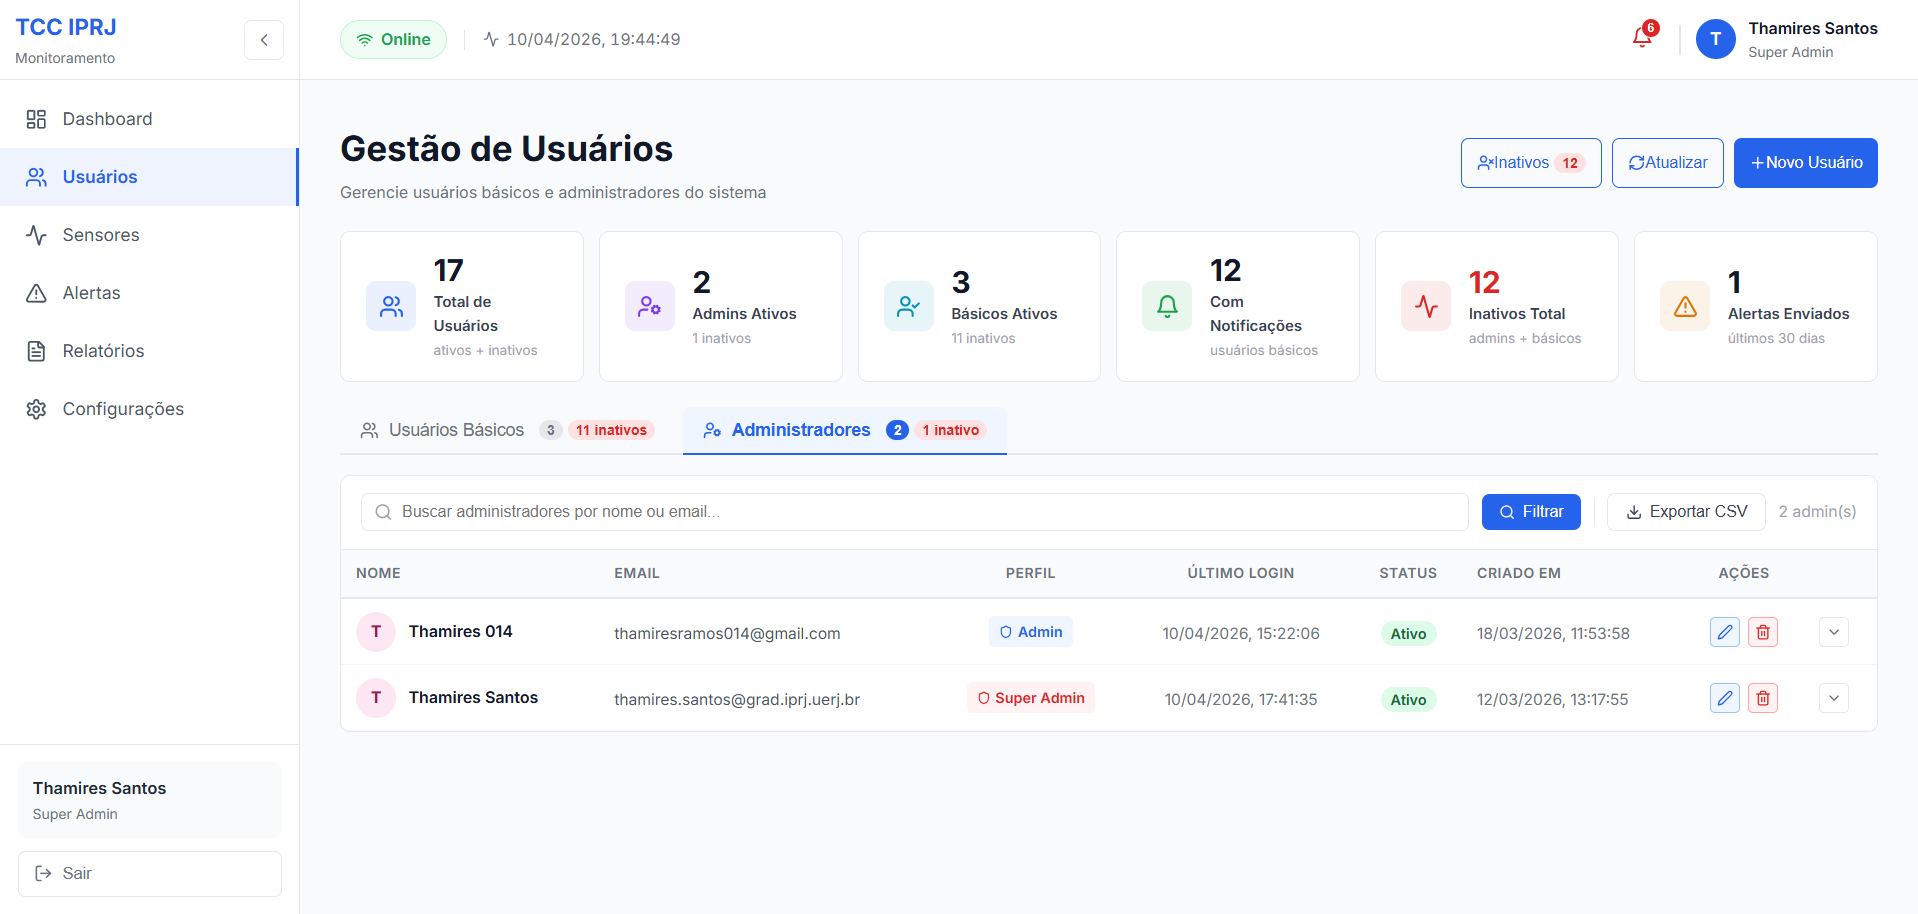
\includegraphics[width=0.85\textwidth]
        {figures/cap5_usuarios_admins.png}
    \caption{Tela de Gestão de Usuários após alternância para a
    aba \textbf{"Administradores"} (perfil \texttt{super\_admin}):
    lista recarregada, filtros limpos e opções de exportação
    atualizadas para o contexto de administradores.}
    \label{fig:usuarios_aba_admins}
    \fonte{Elaborado pela autora.}
\end{figure}

Quando a busca não encontra resultado, o sistema exibe o \textit{toast} ``Erro ao carregar usuários'', 
conforme ilustra a \autoref{fig:usuarios_filtro_sem_resultado}. 
O botão ``Limpar'' remove o filtro e recarrega a lista completa. Administradores sem perfil \textit{super\_admin}
que acessam a aba de Administradores visualizam a tabela, mas os botões
de editar e desativar ficam desabilitados, conforme ilustra a \autoref{fig:usuarios_admins_sem_permissao}.

\begin{figure}[htbp]
    \centering
    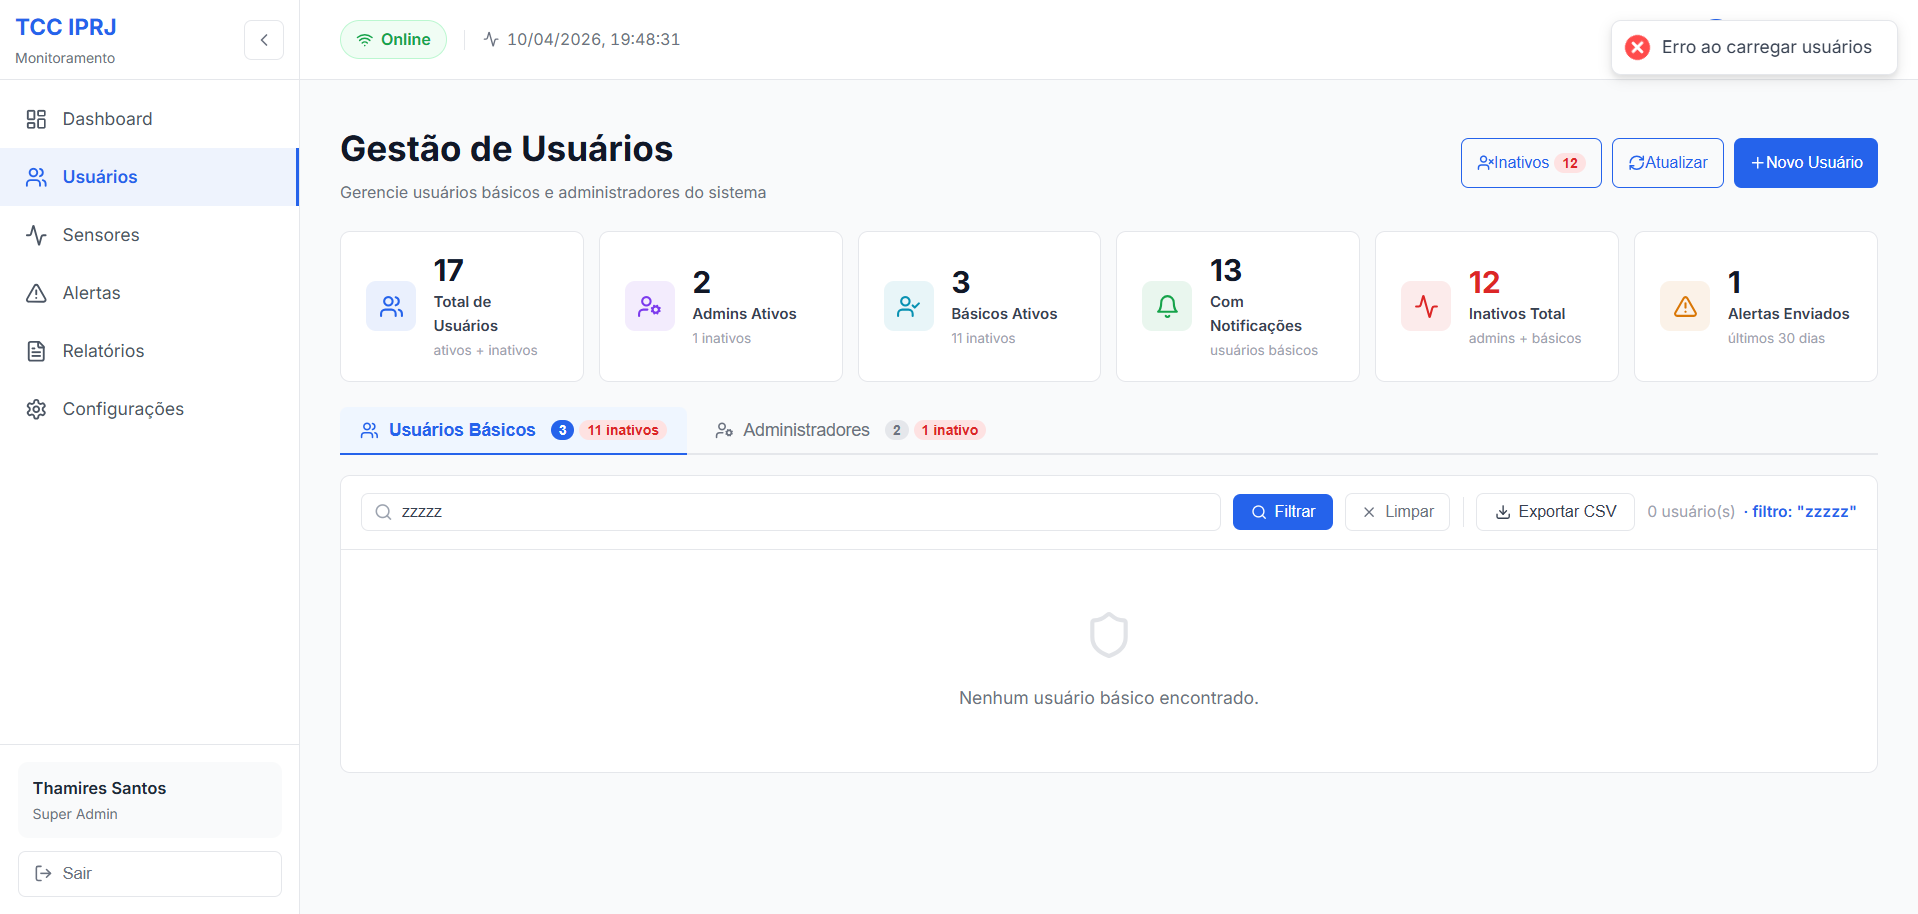
\includegraphics[width=0.95\textwidth]{figures/cap5_usuarios_filtro_sem_resultado.png}
    \caption{Tela de Gestão de Usuários com busca sem resultado: \textit{toast} ``Erro ao carregar usuários'' e tabela em estado vazio; botão ``Limpar'' disponível para remover o filtro aplicado.}
    \label{fig:usuarios_filtro_sem_resultado}
    \fonte{Elaborado pela autora.}
\end{figure}

\begin{figure}[htbp]
    \centering
    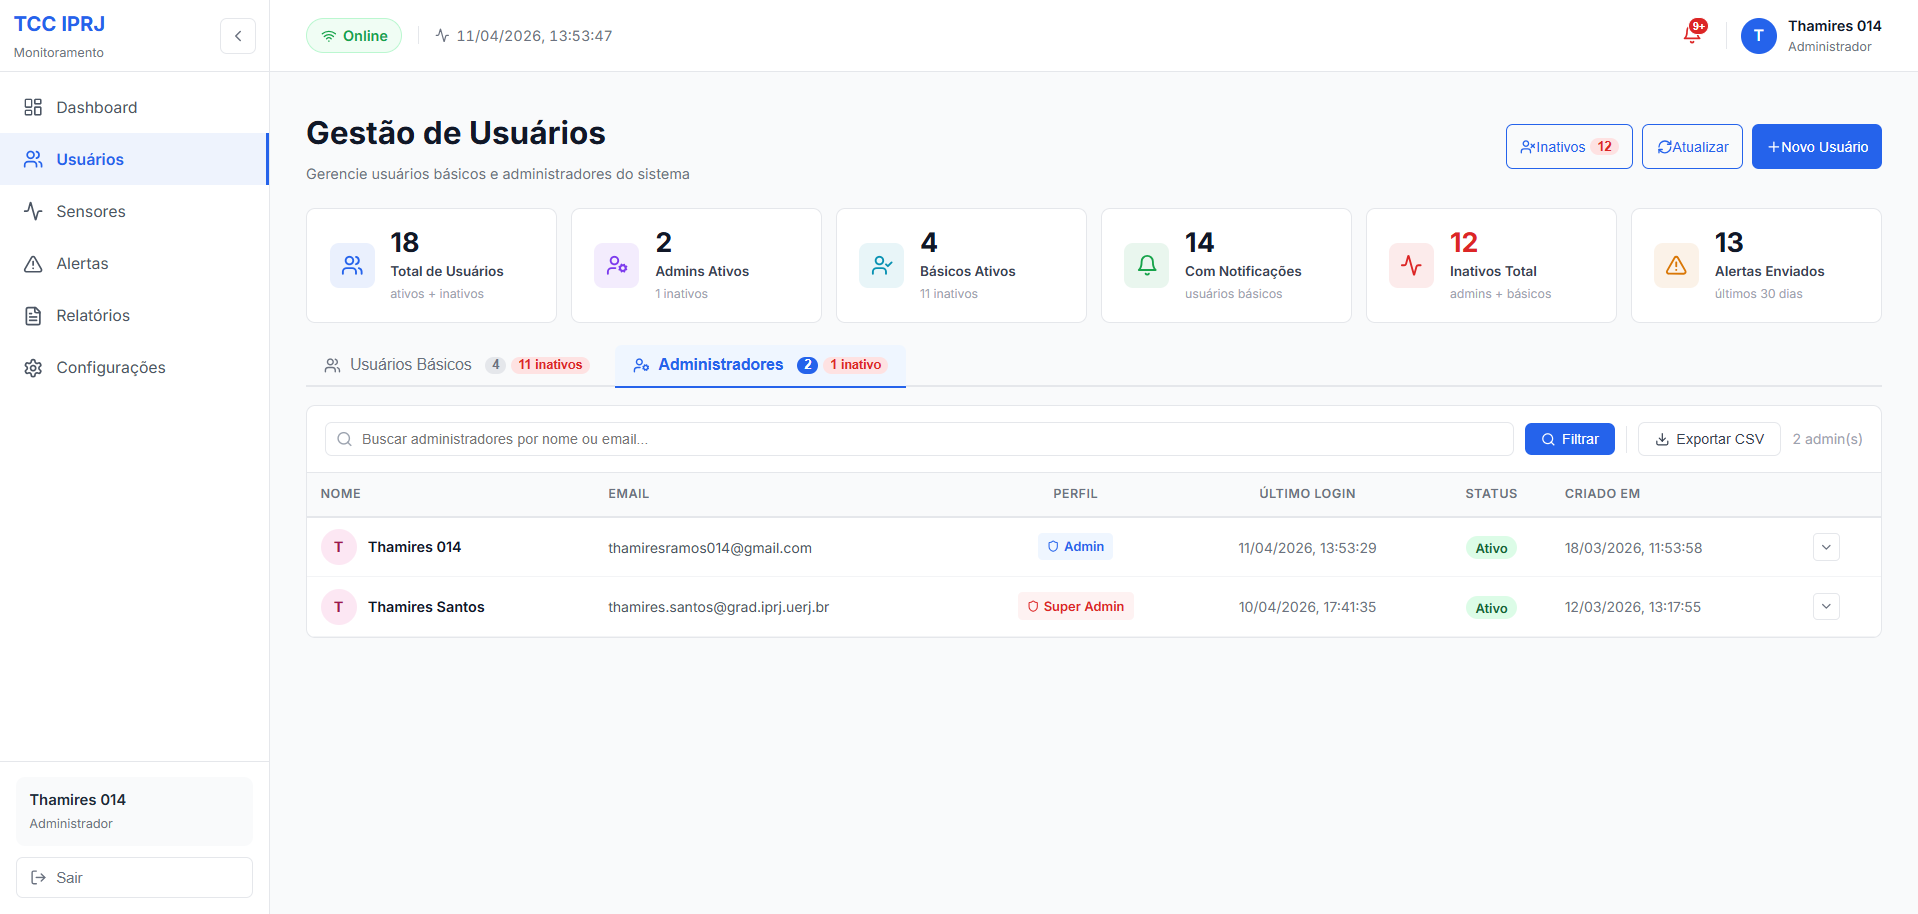
\includegraphics[width=0.95\textwidth]{figures/cap5_usuarios_admins_sem_permissao.png}
    \caption{Aba ``Administradores'' acessada por conta sem perfil
    \textit{super\_admin}: botões de editar e desativar desabilitados
    na tabela; ações de gerenciamento bloqueadas para o perfil sem
    privilégios elevados.}
    \label{fig:usuarios_admins_sem_permissao}
    \fonte{Elaborado pela autora.}
\end{figure}

O botão ``Usuários Inativos'' no cabeçalho da tela abre o modal de
inativos com a lista de contas desativadas e a data de desativação de
cada uma, permitindo reativá-las individualmente com um clique, conforme ilustra a \autoref{fig:usuarios_inativos_modal}.

\begin{figure}[htbp]
    \centering
    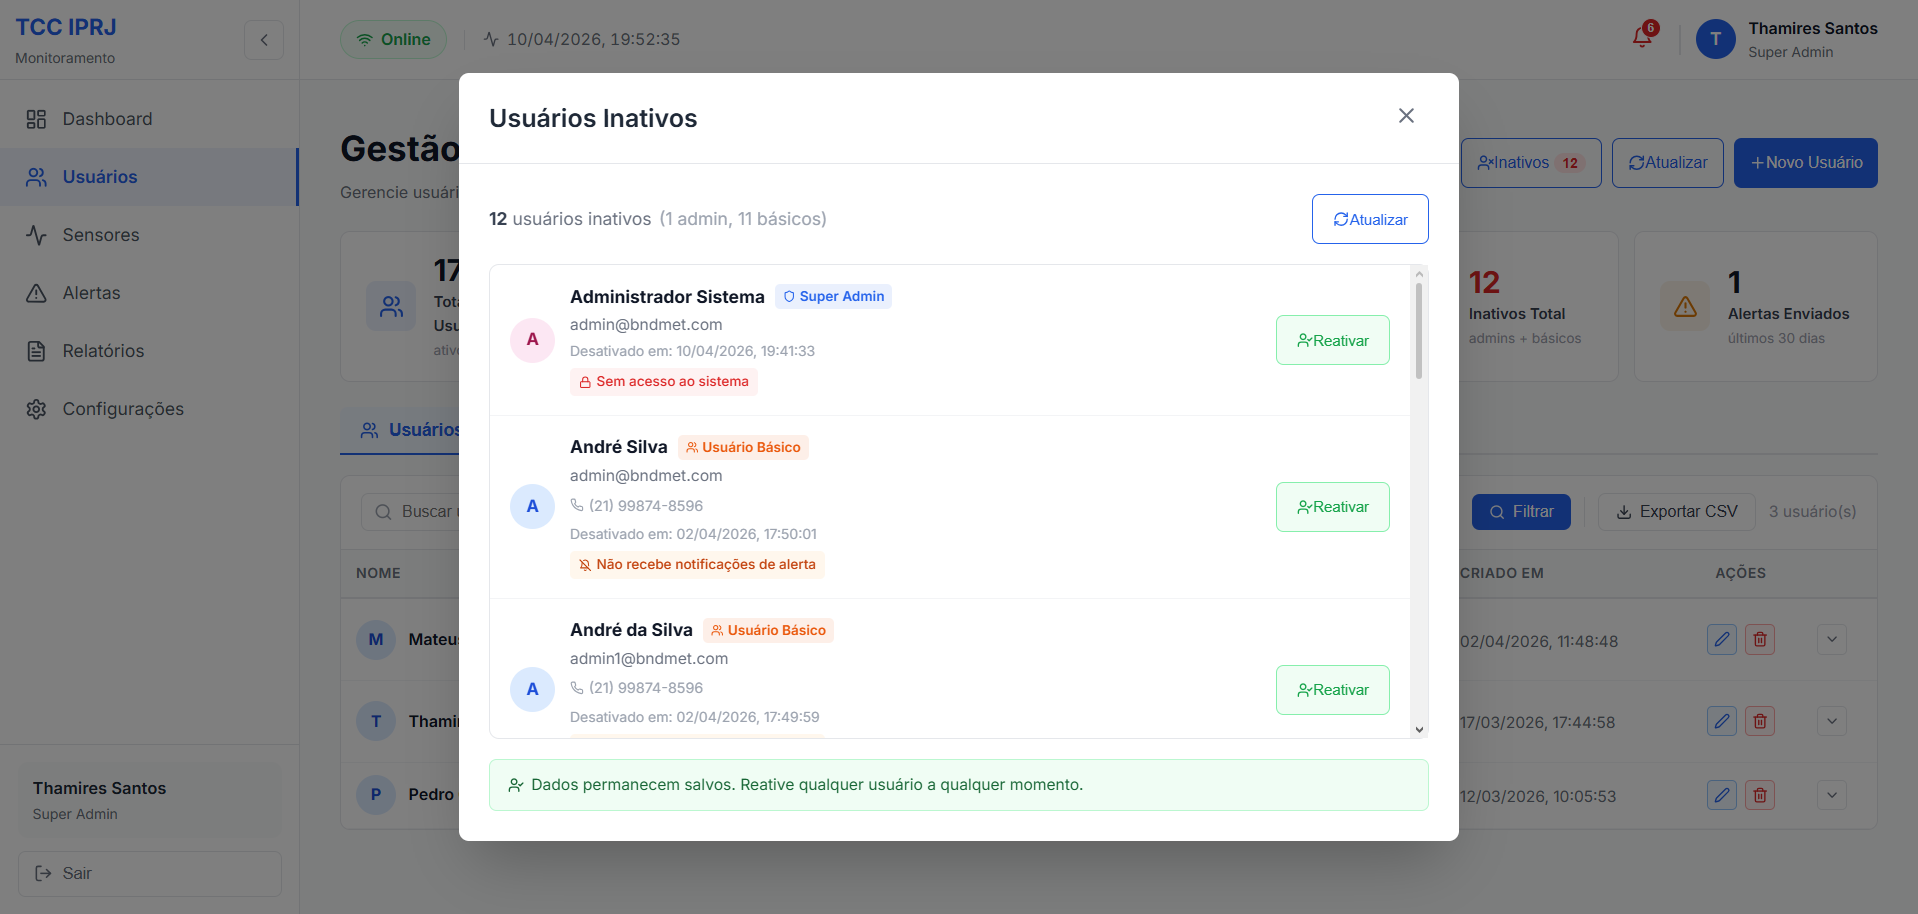
\includegraphics[width=0.85\textwidth]{figures/cap5_usuarios_inativos_modal.png}
    \caption{Modal de Usuários Inativos: lista de contas desativadas com data de desativação e botão ``Reativar'' por linha.}
    \label{fig:usuarios_inativos_modal}
    \fonte{Elaborado pela autora.}
\end{figure}

% -------------------------------------------------------------
\subsection{Criação e Edição de Usuário}
\label{subsec:usuarios-crud}
% -------------------------------------------------------------

O modal de criação é aberto pelo botão ``Novo Usuário'' no cabeçalho.
Para usuários básicos, o formulário apresenta os campos nome, e-mail,
telefone com máscara automática e \textit{toggle} de preferência de
notificações. Para administradores, os campos são nome, e-mail, senha,
confirmação de senha e perfil. As \autoref{fig:usuario_form} e \autoref{fig:usuario_form_adm} exibem o
formulário de criação de usuário básico e super administrador preenchido, respectivamente.

\begin{figure}[htbp]
    \centering
    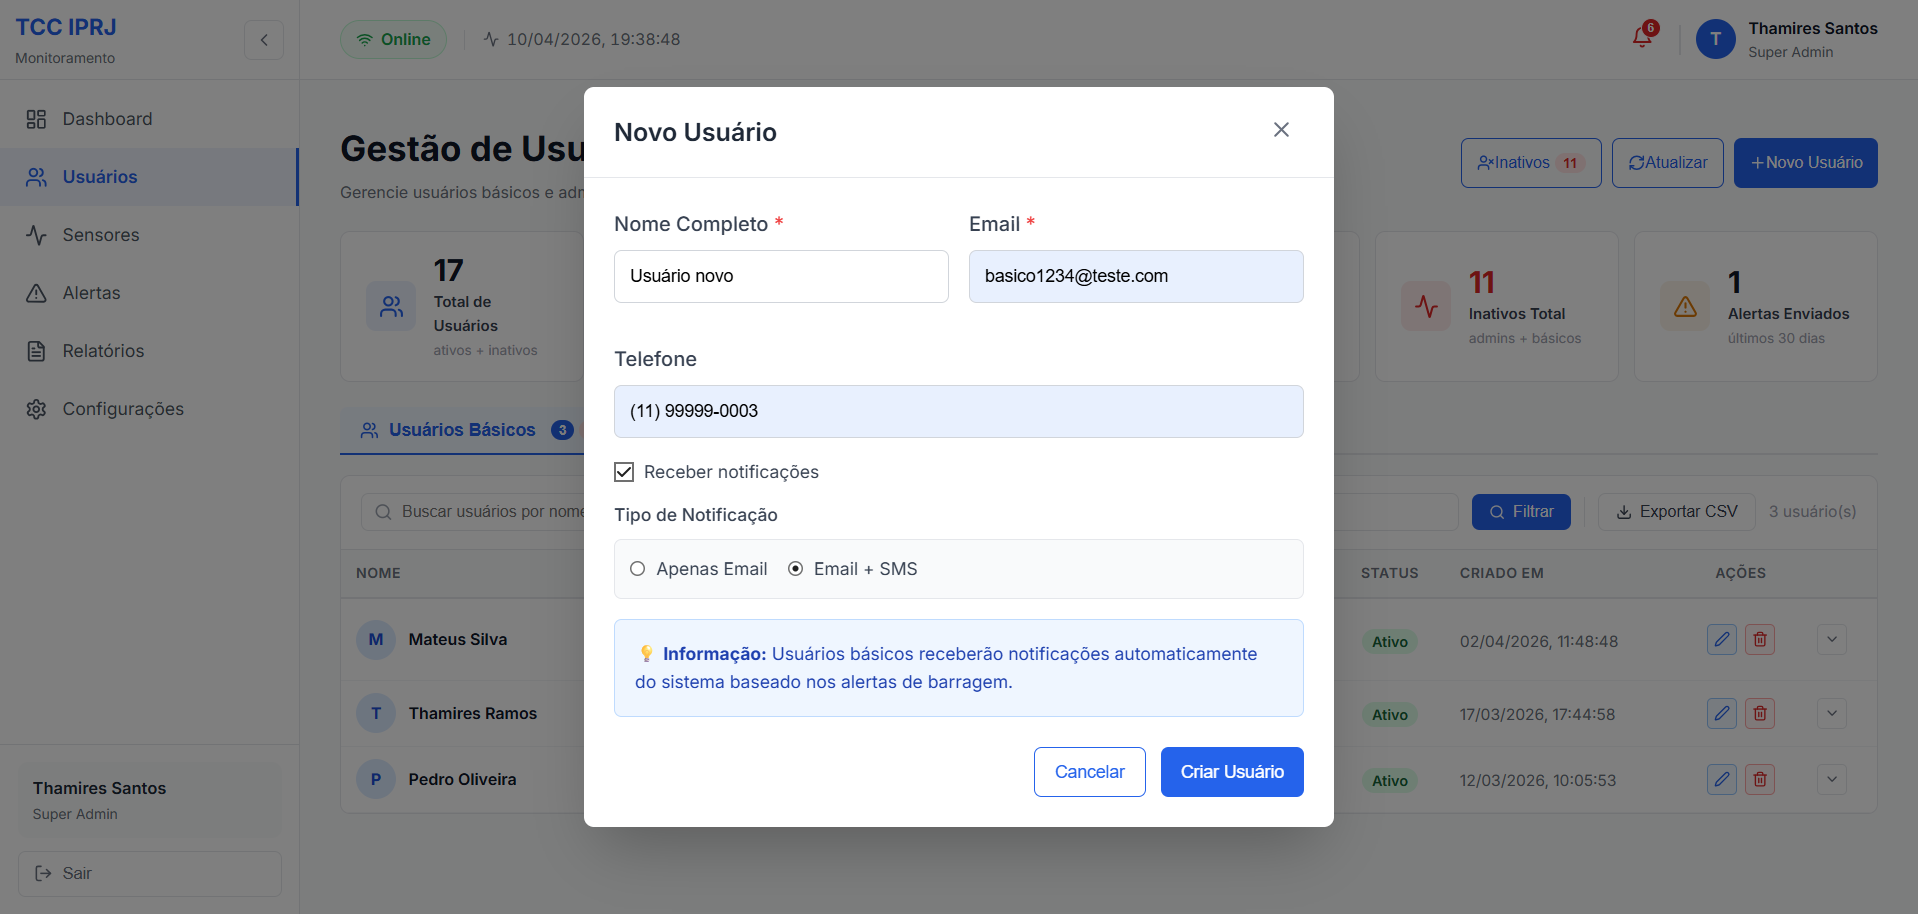
\includegraphics[width=0.75\textwidth]{figures/cap5_usuario_form.png}
    \caption{Formulário de criação de usuário básico: campos de nome,
    e-mail, telefone com máscara automática e \textit{toggle} de
    notificações.}
    \label{fig:usuario_form}
    \fonte{Elaborado pela autora.}
\end{figure}

\begin{figure}[htbp]
    \centering
    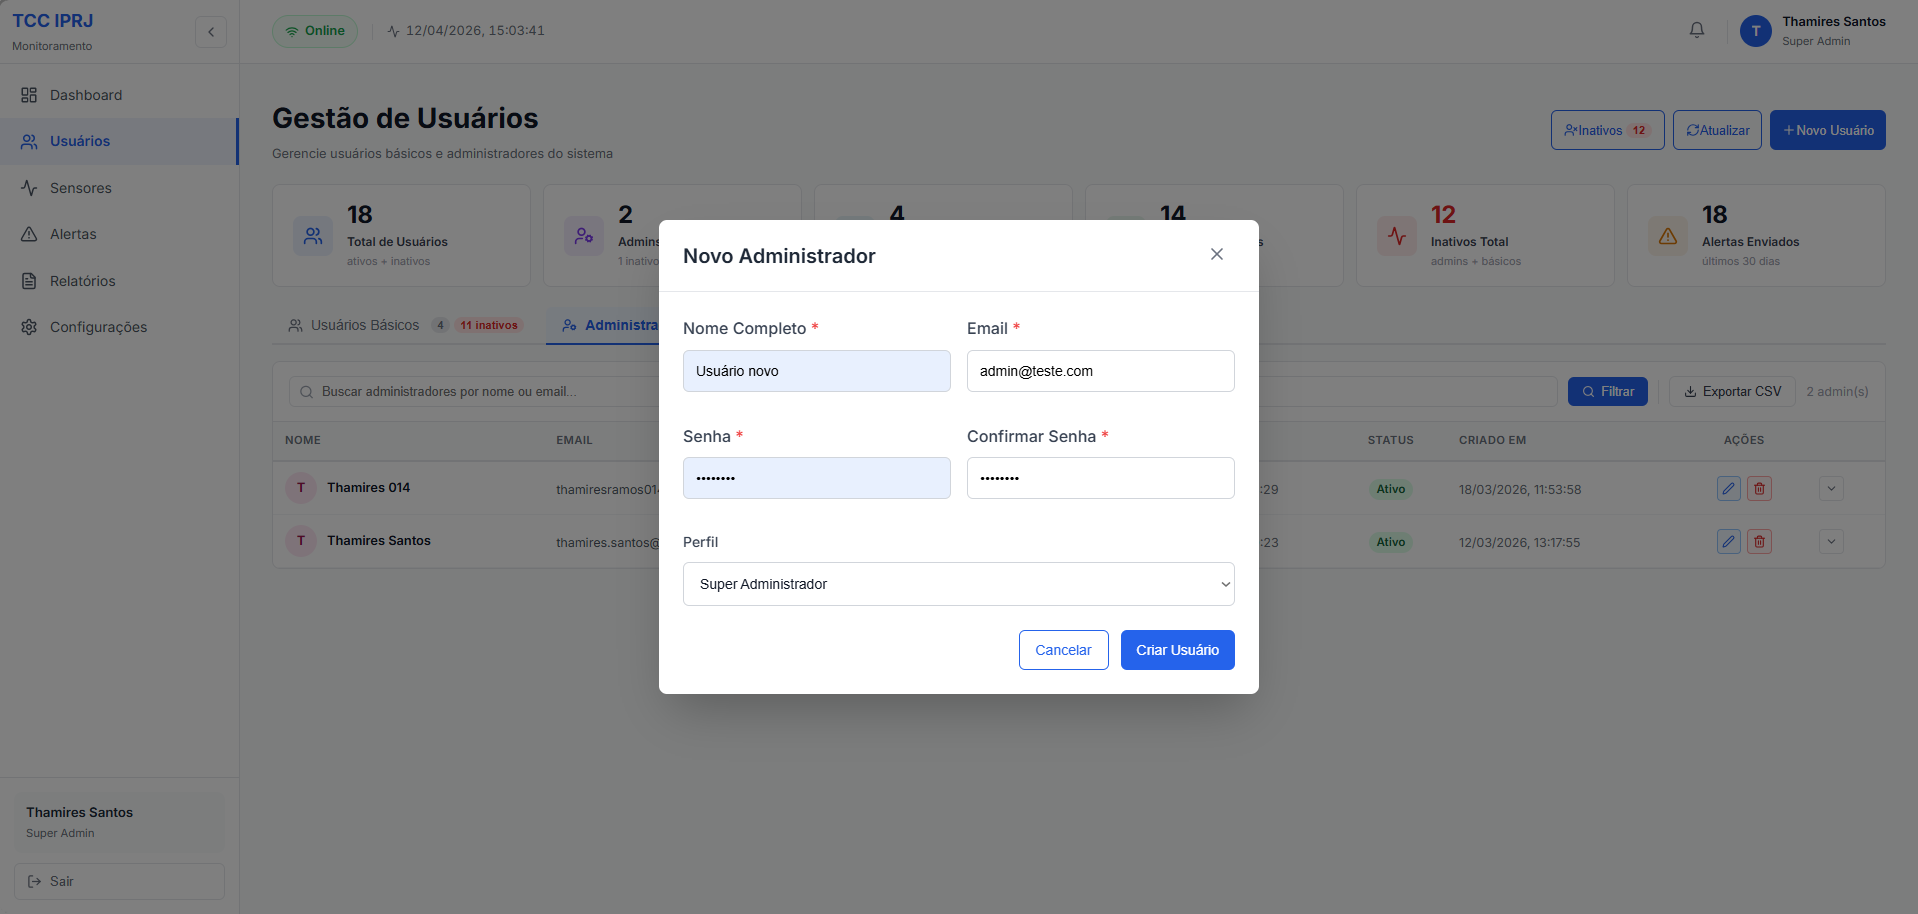
\includegraphics[width=0.75\textwidth]{figures/cap5_usuario_form_adm.png}
    \caption{Formulário de criação de usuário super administrador: campos de nome,
    e-mail, senha, confirmação de senha e perfil.}
    \label{fig:usuario_form_adm}
    \fonte{Elaborado pela autora.}
\end{figure}

Ao salvar, o \textit{toast} ``Usuário criado com sucesso'' confirma a
operação e a lista é recarregada. Quando o e-mail já está cadastrado, o
\textit{backend} retorna HTTP 400 e o sistema exibe a mensagem de erro,
mantendo o formulário aberto para correção, conforme ilustra a \autoref{fig:usuario_criacao_email_duplicado}.

\begin{figure}[htbp]
    \centering
    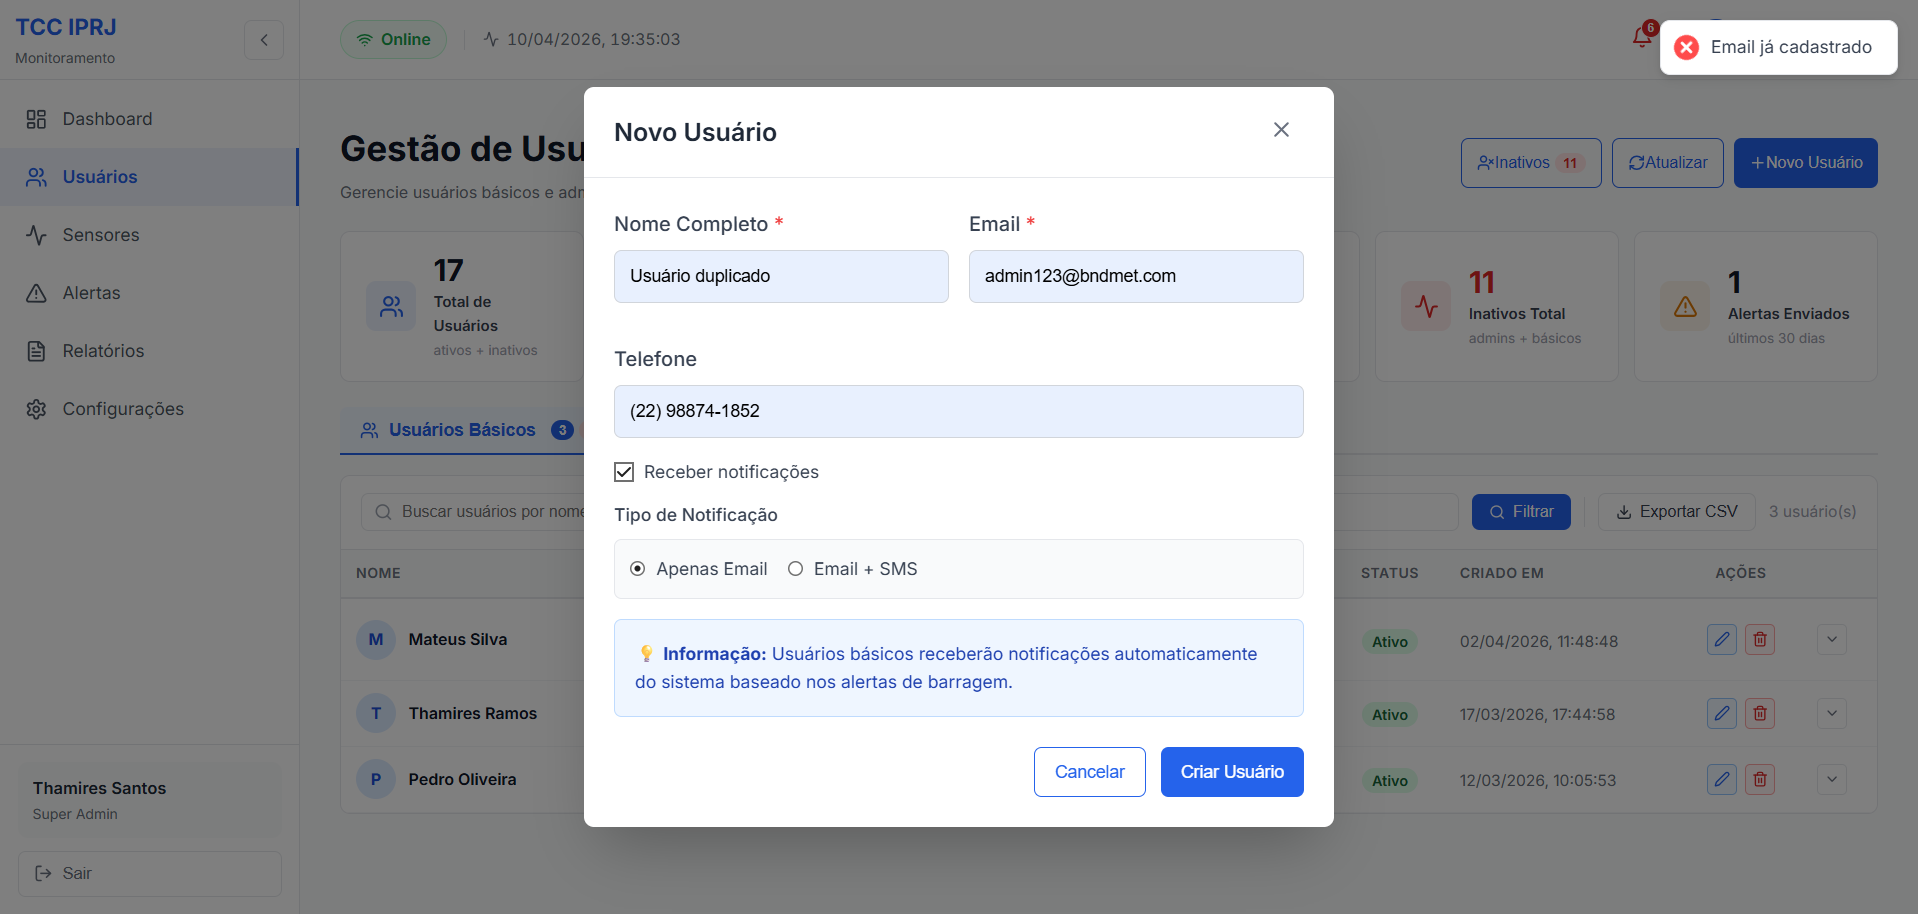
\includegraphics[width=0.75\textwidth]{figures/cap5_usuario_criacao_email_duplicado.png}
    \caption{Formulário de criação de usuário básico com \textit{toast} de e-mail duplicado: \textit{backend} retorna HTTP 400 ``Email já cadastrado''; formulário mantido aberto para correção.}
    \label{fig:usuario_criacao_email_duplicado}
    \fonte{Elaborado pela autora.}
\end{figure}

A edição segue o mesmo
fluxo, com o formulário pré-preenchido com os dados atuais do usuário
selecionado, conforme ilustra a \autoref{fig:usuario_edicao_email_duplicado}.

\begin{figure}[htbp]
    \centering
    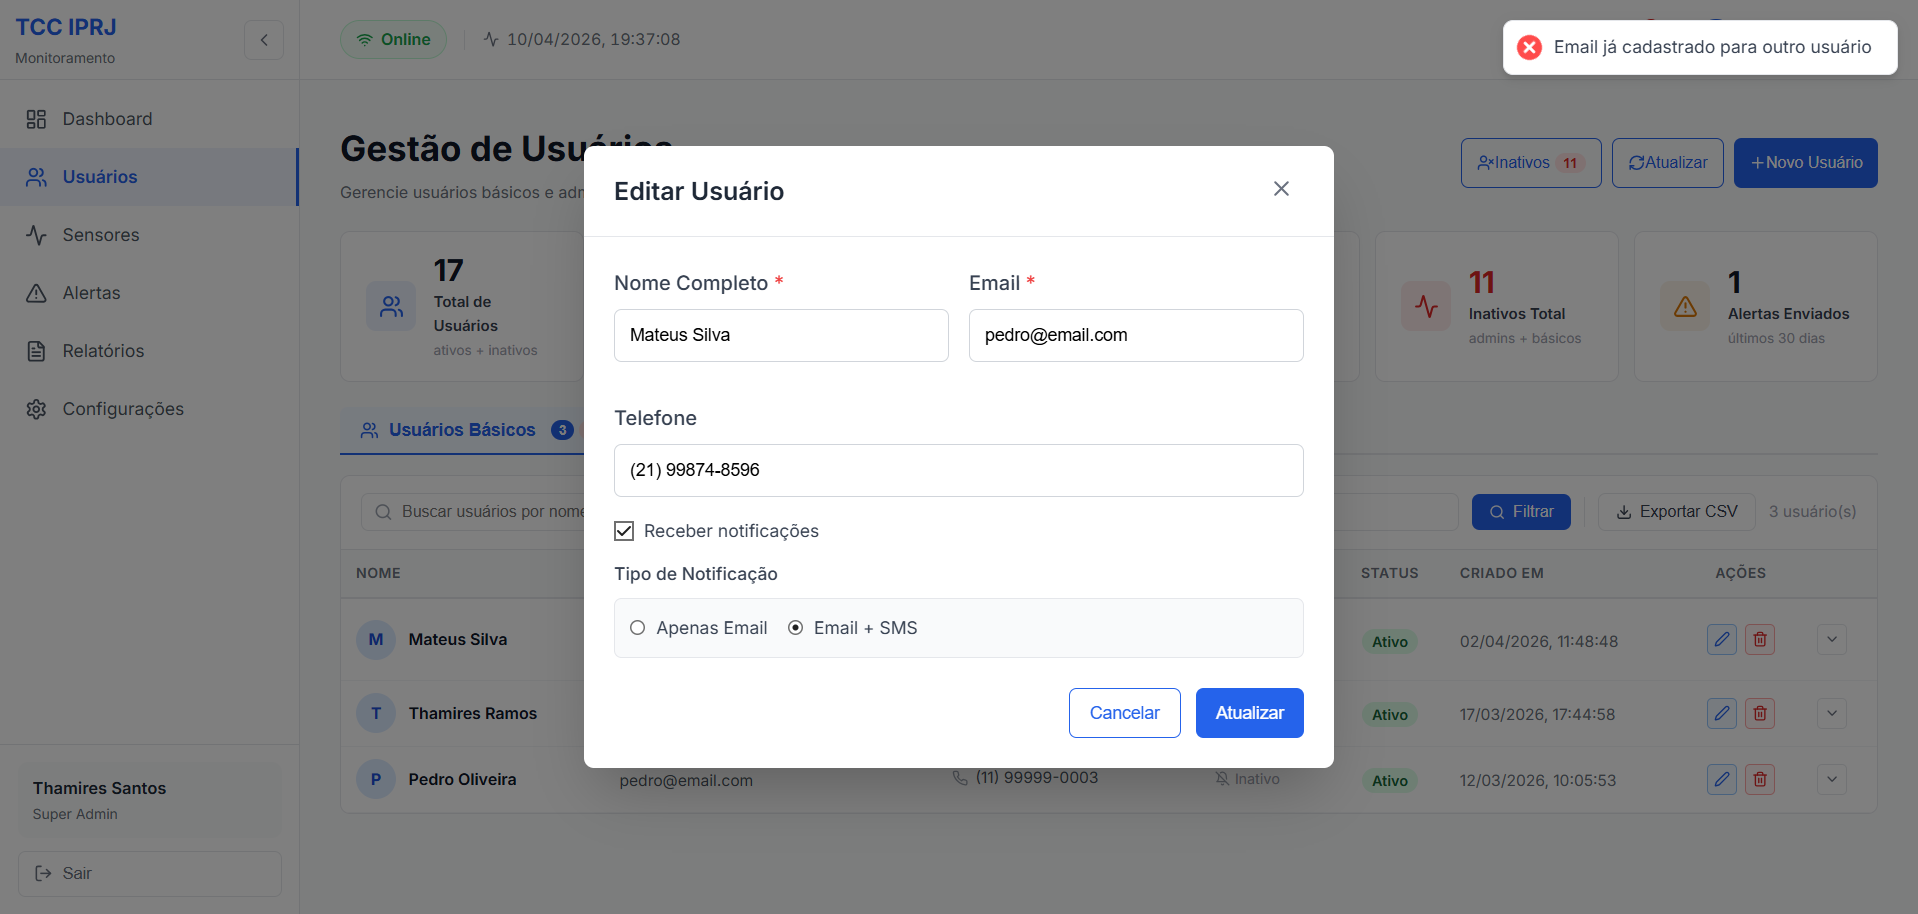
\includegraphics[width=0.75\textwidth]{figures/cap5_usuario_edicao_email_duplicado.png}
    \caption{Formulário de edição de usuário básico com \textit{toast} de conflito de e-mail: endereço já em uso por outro usuário; formulário pré-preenchido retorna para correção.}
    \label{fig:usuario_edicao_email_duplicado}
    \fonte{Elaborado pela autora.}
\end{figure}

% -------------------------------------------------------------
\subsection{Ativação e Desativação de Usuário}
\label{subsec:usuarios-ativacao}
% -------------------------------------------------------------

A desativação é sempre lógica --- o registro não é removido do banco ---,
preservando o histórico de destinatários nos registros de alertas enviados.
Ao clicar no botão de desativar, o modal de confirmação exibe o nome do
usuário e as consequências da ação: usuários básicos deixam de receber
notificações; administradores perdem o acesso ao painel, conforme mostra a \autoref{fig:usuario_modal_desativacao_pt1}. O administrador
confirma ou cancela; em caso de confirmação, o \textit{toast} ``Usuário
desativado!'' é exibido e a lista é recarregada, conforme ilustra a \autoref{fig:usuario_modal_desativacao_pt2}.

\begin{figure}[htbp]
    \centering
    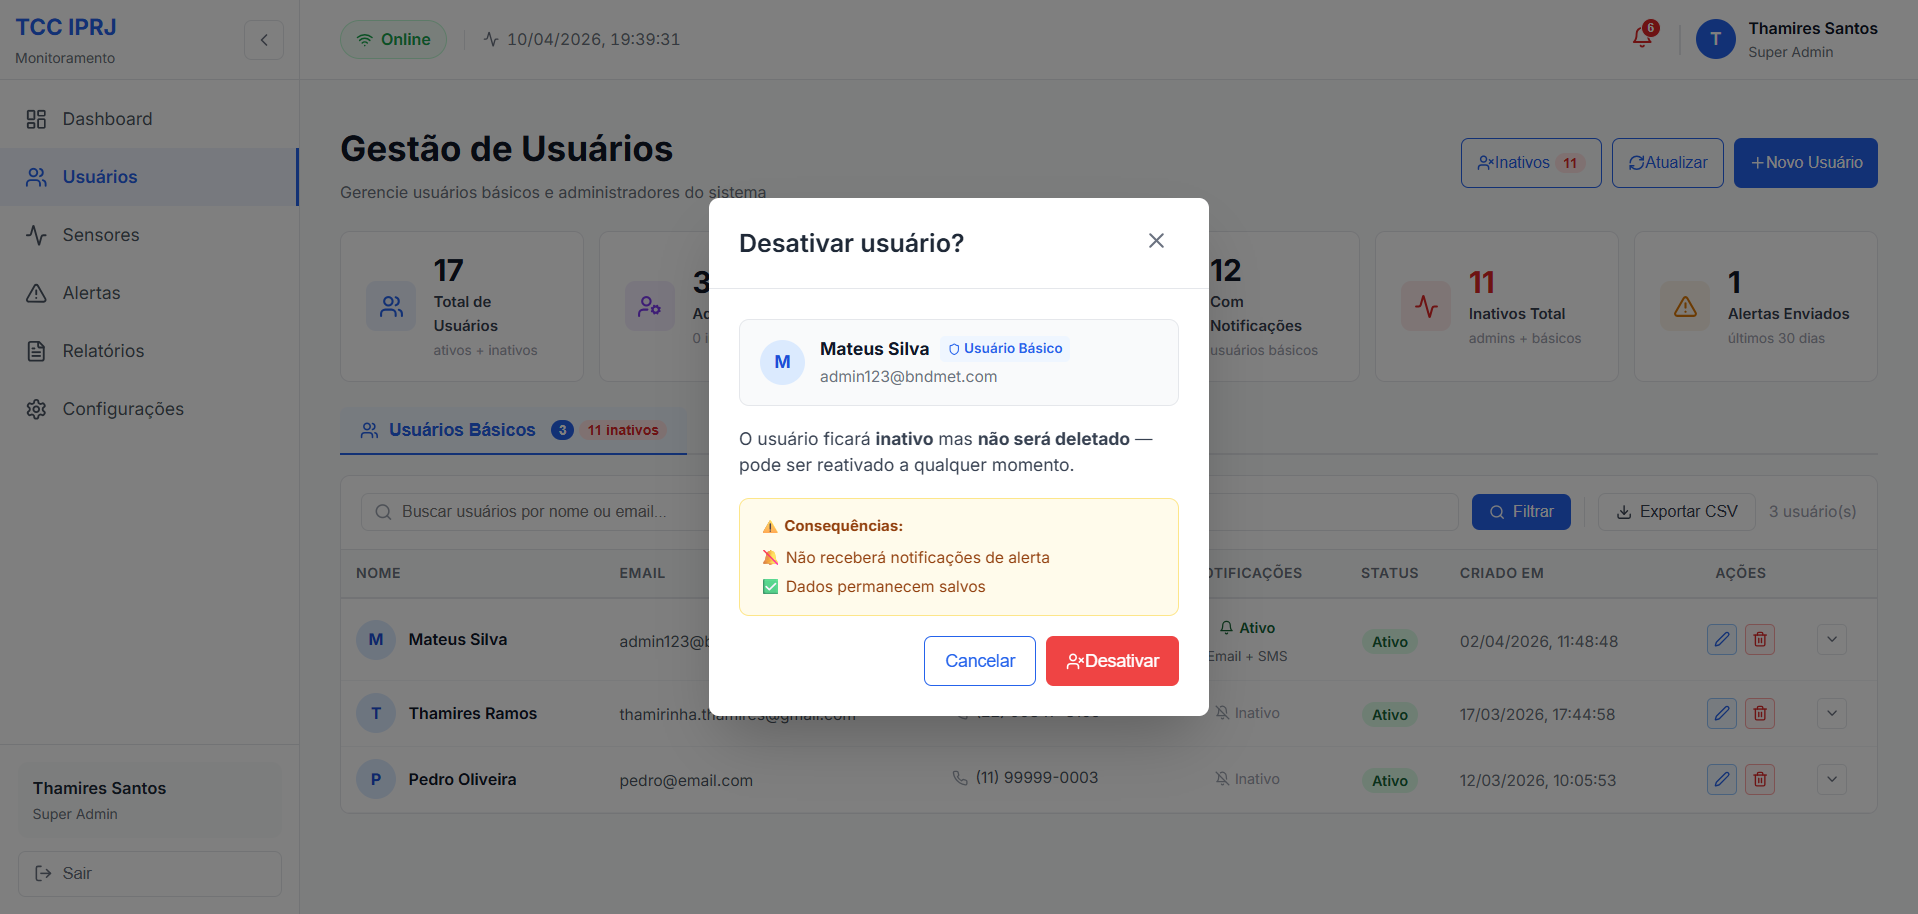
\includegraphics[width=0.75\textwidth]{figures/cap5_usuario_modal_desativacao_pt1.png}
    \caption{Modal de confirmação de desativação de usuário: nome do usuário, consequências da ação (perda de notificações ou de acesso ao painel) e botões ``Confirmar'' e ``Cancelar''.}
    \label{fig:usuario_modal_desativacao_pt1}
    \fonte{Elaborado pela autora.}
\end{figure}

\begin{figure}[htbp]
    \centering
    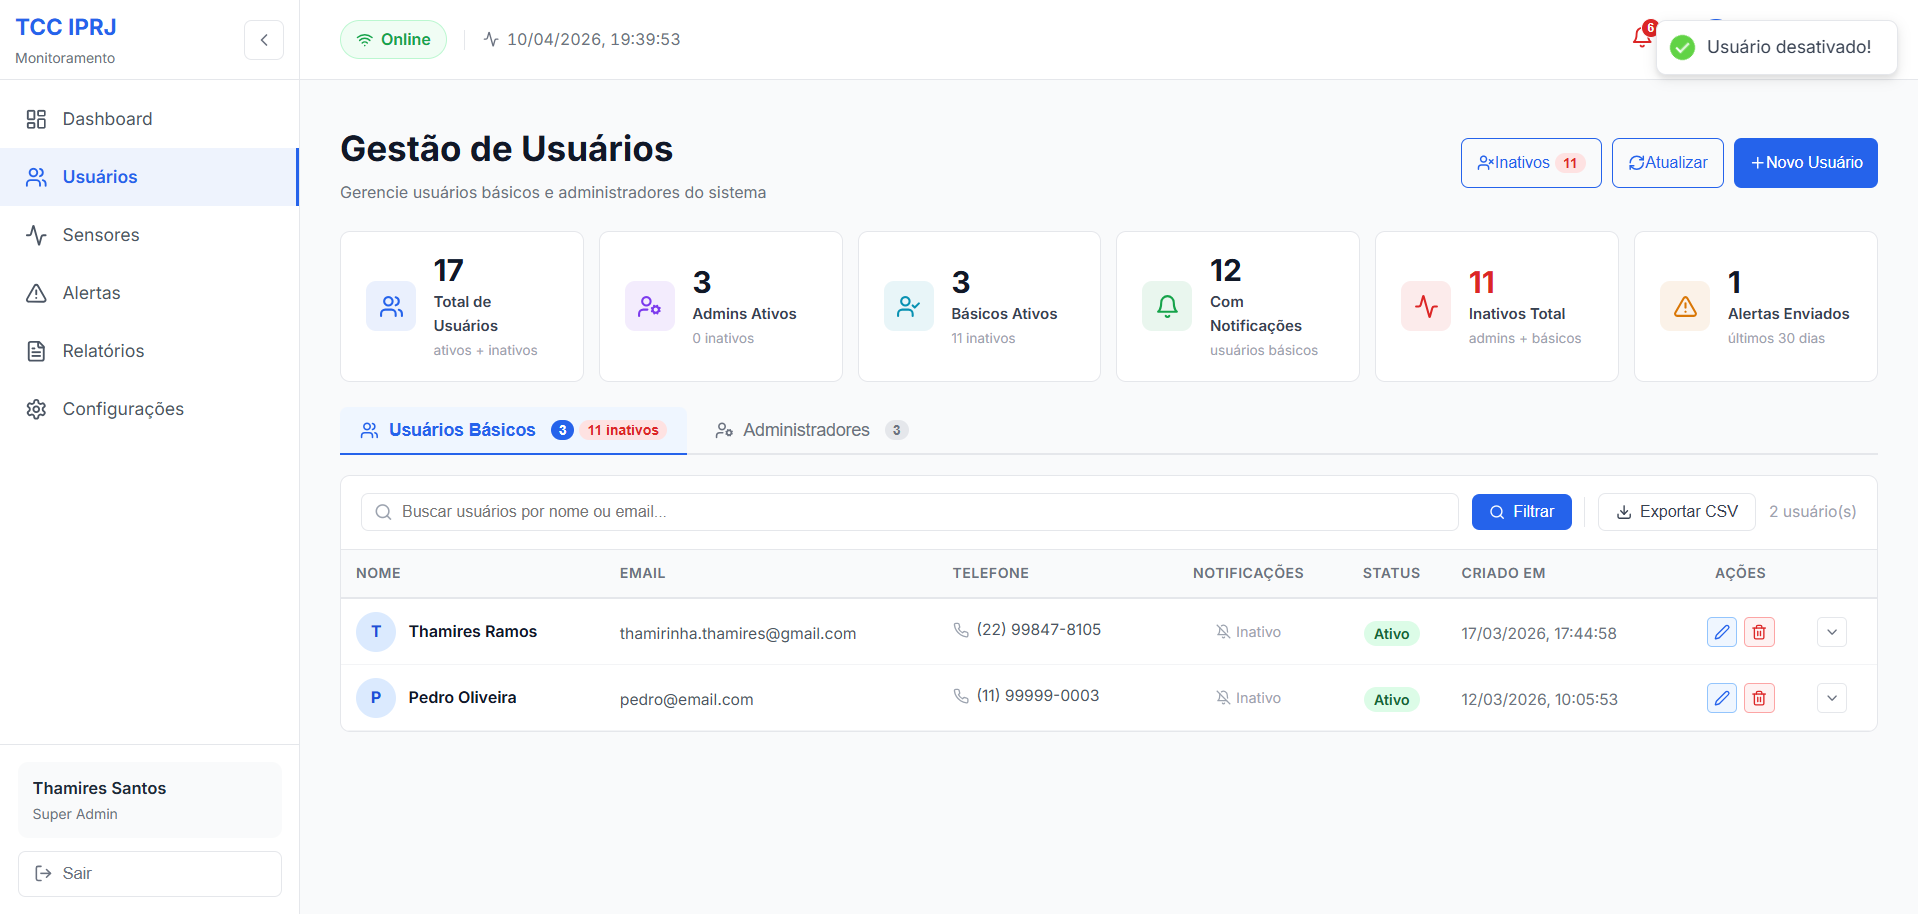
\includegraphics[width=0.75\textwidth]{figures/cap5_usuario_modal_desativacao_pt2.png}
    \caption{\textit{toast} ``Usuário desativado!'' e lista de usuários recarregada.}
    \label{fig:usuario_modal_desativacao_pt2}
    \fonte{Elaborado pela autora.}
\end{figure}

A reativação é realizada pelo modal de usuários inativos: ao clicar em
``Reativar'', o \textit{toast} ``Usuário reativado com sucesso!'' confirma
a operação e o usuário desaparece da lista de inativos, conforme ilustram
as \autoref{fig:usuario_reativacao_toast_pt1},
\autoref{fig:usuario_reativacao_toast_pt2} e
\autoref{fig:usuario_reativacao_toast_pt3}.

\begin{figure}[htbp]
    \centering
    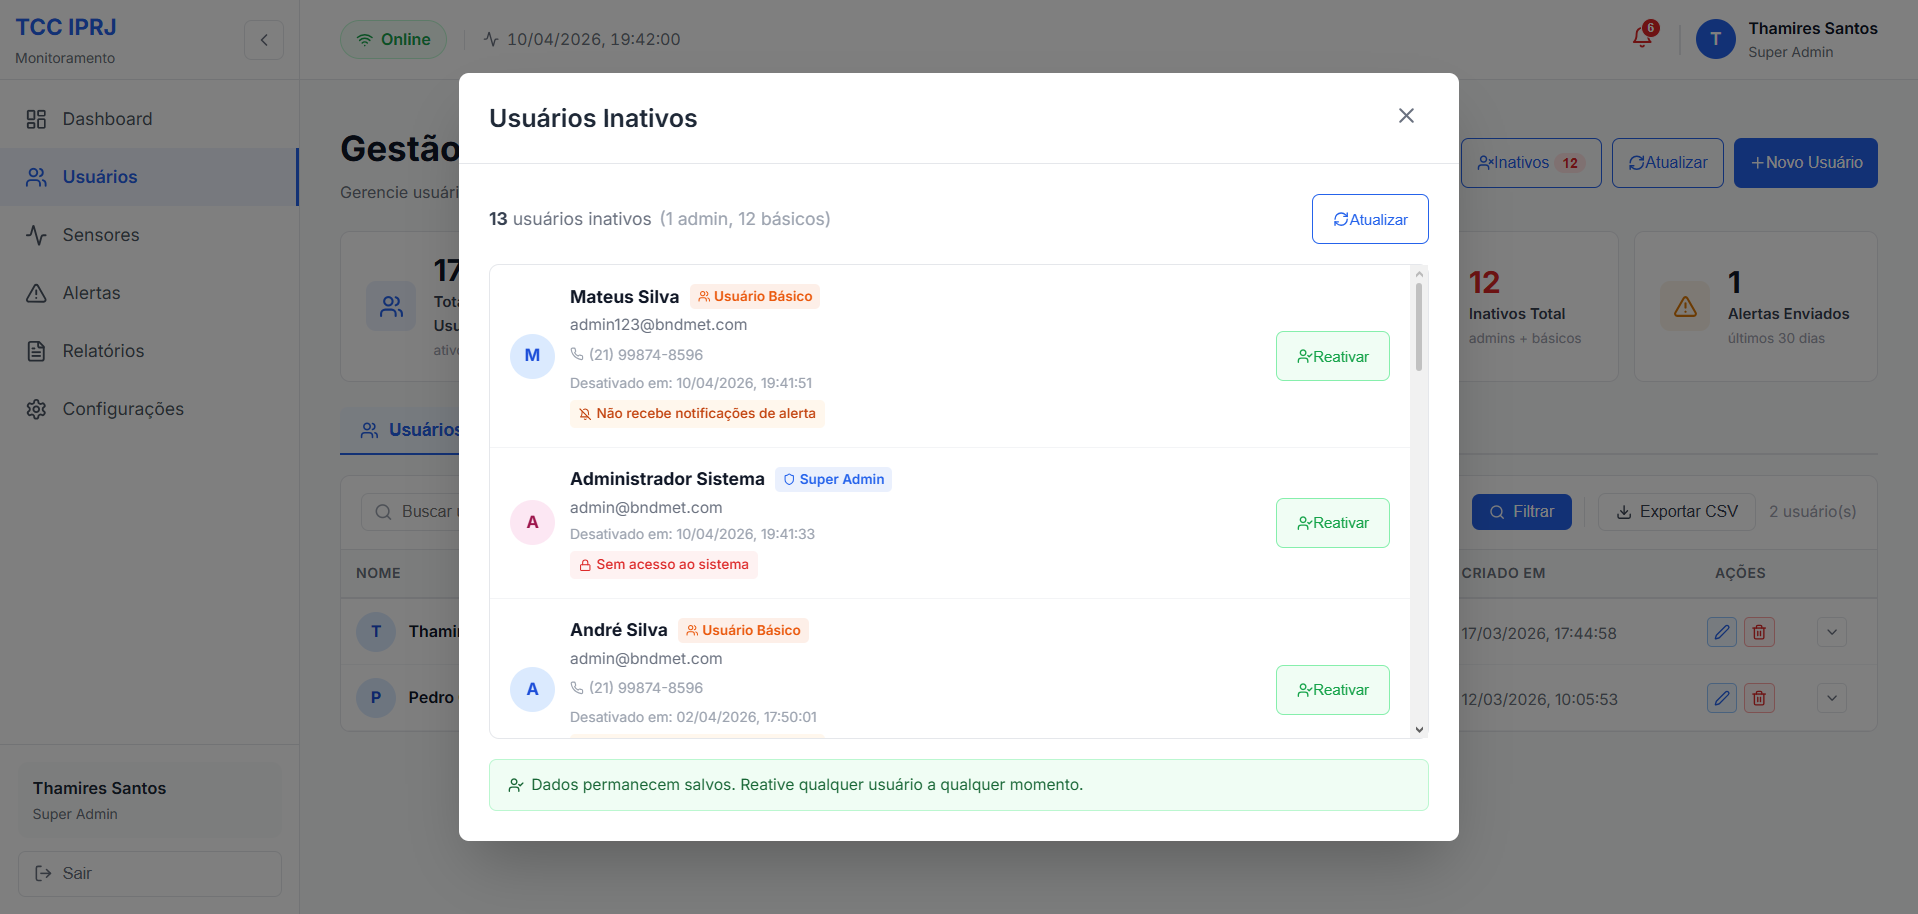
\includegraphics[width=0.85\textwidth]{figures/cap5_usuario_reativacao_toast_pt1.png}
    \caption{Modal de Usuários Inativos com reativação em andamento (parte~1): botão ``Reativar'' acionado para o usuário selecionado.}
    \label{fig:usuario_reativacao_toast_pt1}
    \fonte{Elaborado pela autora.}
\end{figure}

\begin{figure}[htbp]
    \centering
    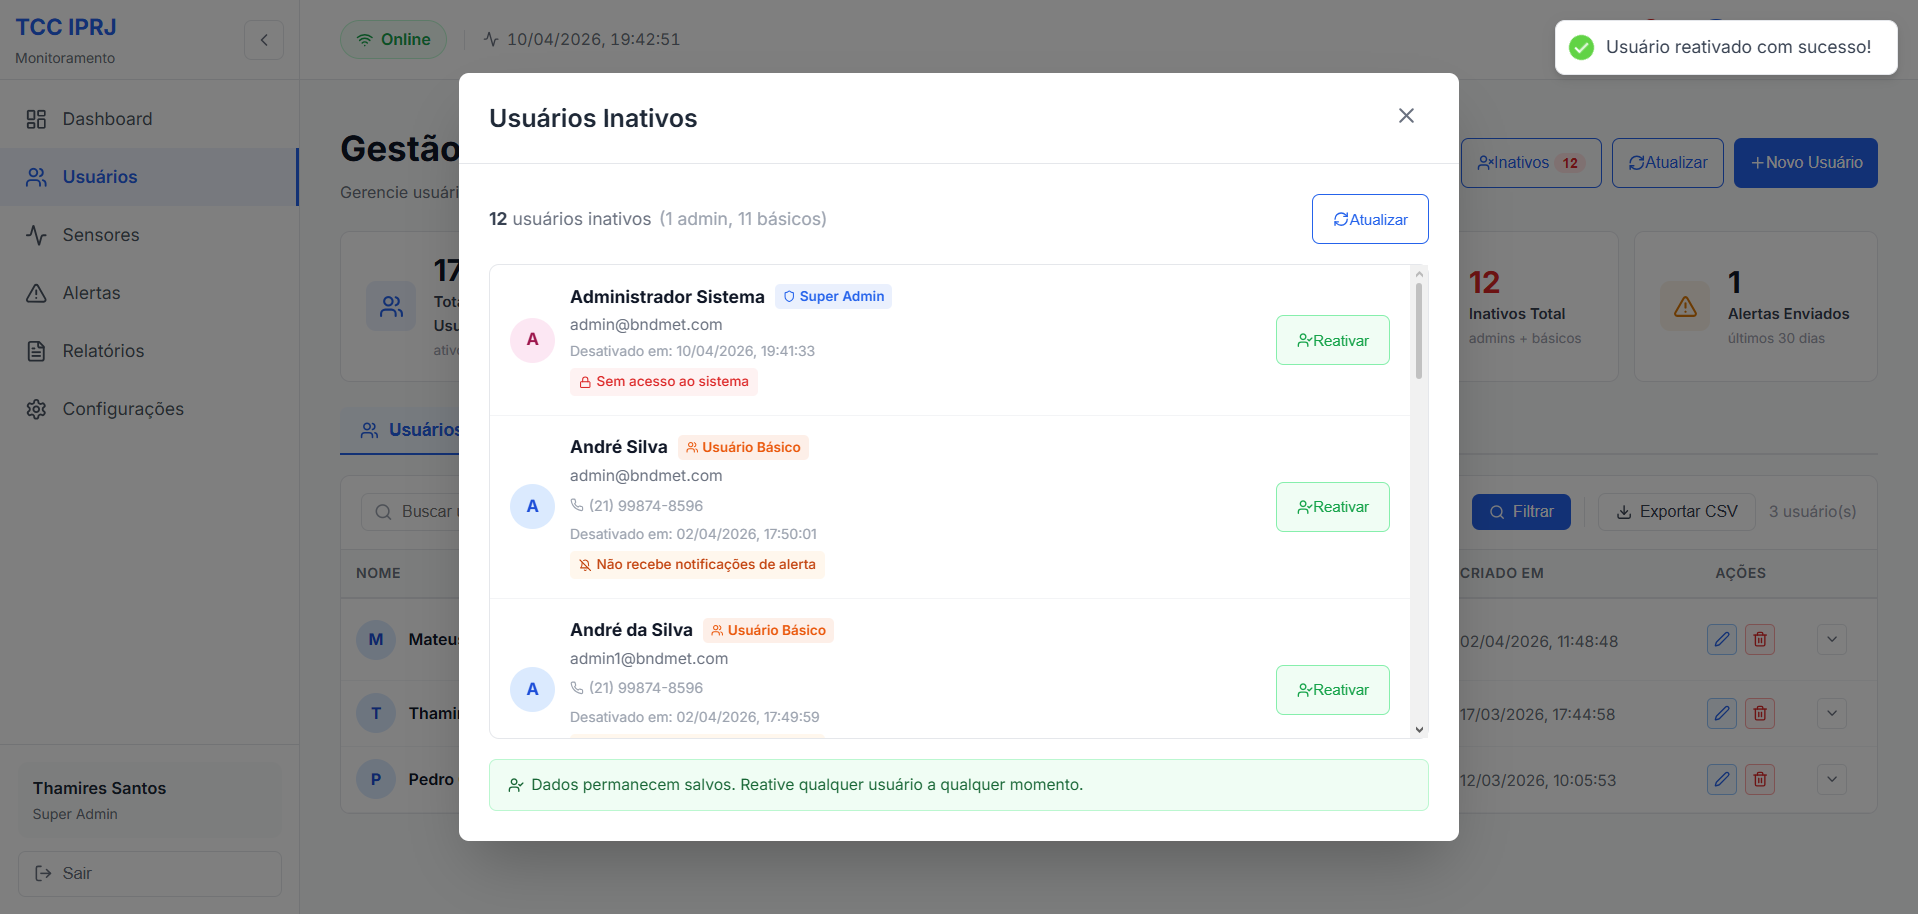
\includegraphics[width=0.85\textwidth]{figures/cap5_usuario_reativacao_toast_pt2.png}
    \caption{Modal de Usuários Inativos com reativação em andamento (parte~2): usuário removido da lista de inativos e \textit{toast} ``Usuário reativado com sucesso!'' confirmando a operação.}
    \label{fig:usuario_reativacao_toast_pt2}
    \fonte{Elaborado pela autora.}
\end{figure}

\begin{figure}[htbp]
    \centering
    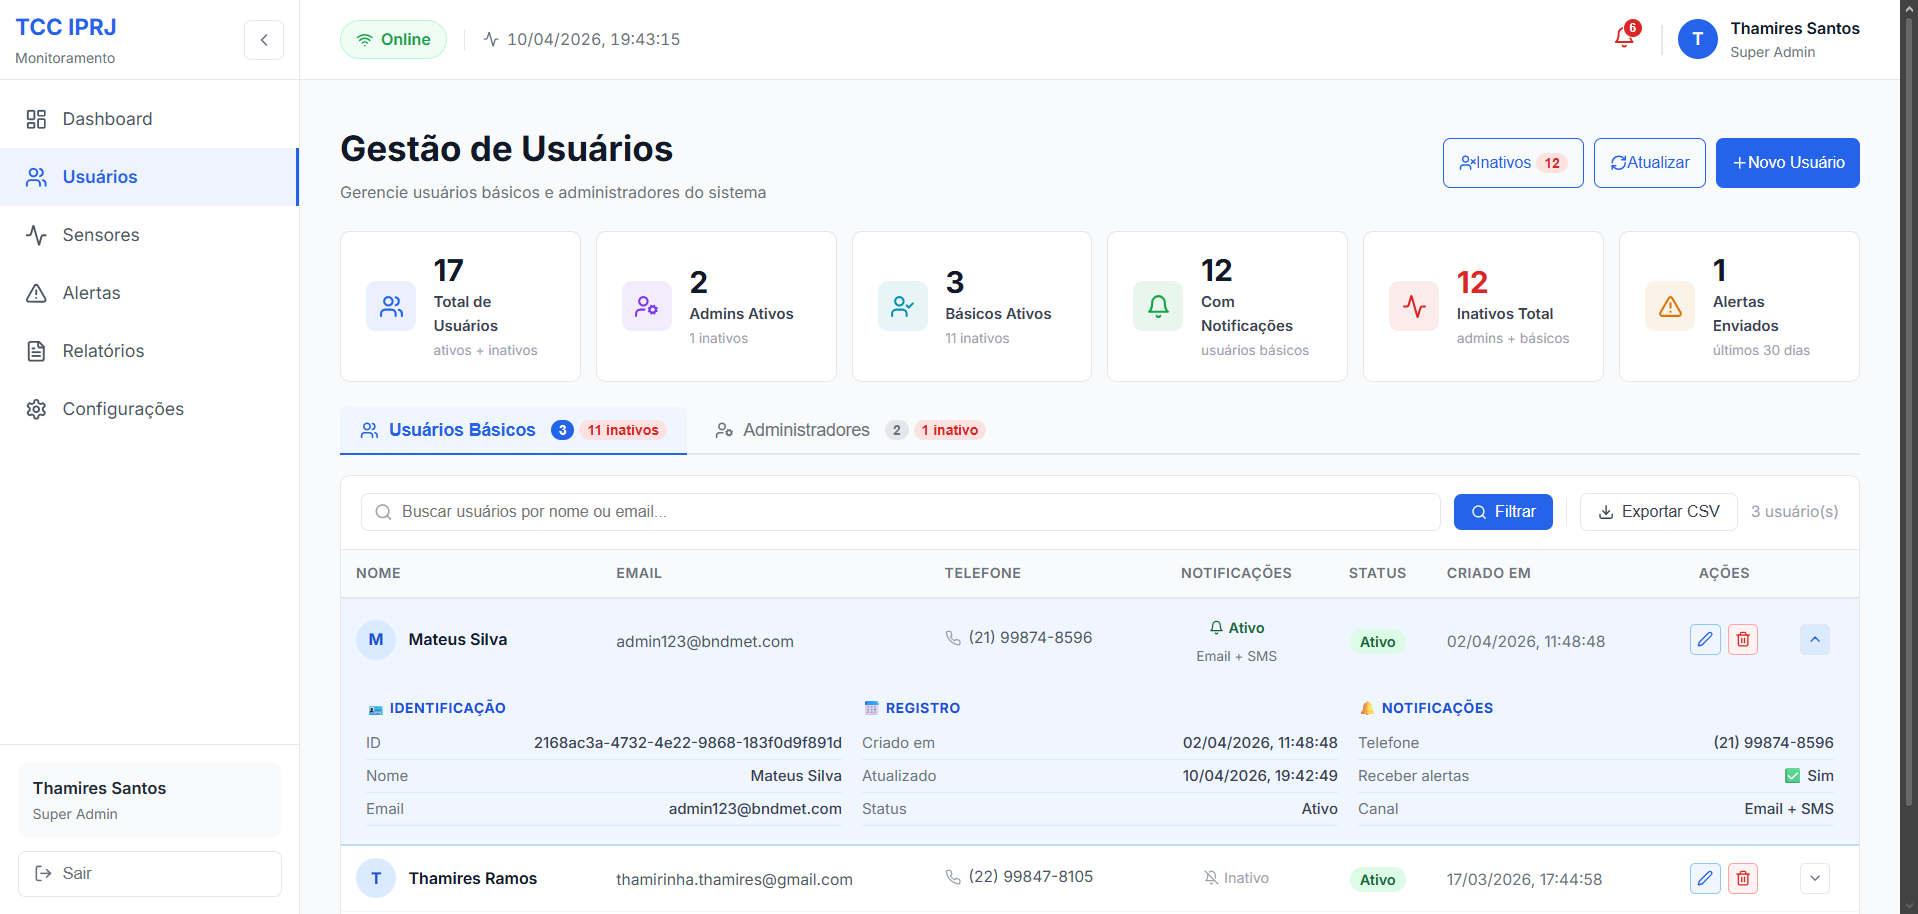
\includegraphics[width=0.85\textwidth]{figures/cap5_usuario_reativacao_toast_pt3.png}
    \caption{Modal de Usuários Inativos após reativação concluída (parte~3): usuário retornado à listagem principal com os dados atualizados.}
    \label{fig:usuario_reativacao_toast_pt3}
    \fonte{Elaborado pela autora.}
\end{figure}

% -------------------------------------------------------------
\subsection{Exportação de Usuários em CSV}
\label{subsec:usuarios-csv}
% -------------------------------------------------------------

O botão ``Exportar CSV'' gera um arquivo com os campos correspondentes
ao tipo de usuário da aba ativa: para básicos, inclui nome, e-mail,
telefone, preferência de notificação, status e datas de criação e
atualização; para administradores, inclui nome, e-mail, perfil, último
\textit{login}, status e datas de criação e
atualização. O nome do arquivo reflete o tipo e a data da
exportação. O \textit{toast} confirma a quantidade de registros
exportados, conforme mostra a \autoref{fig:usuarios_csv_sucesso}. Quando não há dados para exportar, o \textit{toast} ``Nenhum
dado para exportar'' é exibido sem gerar arquivo, conforme ilustra a \autoref{fig:usuarios_csv_sem_dados}.

\begin{figure}[htbp]
    \centering
    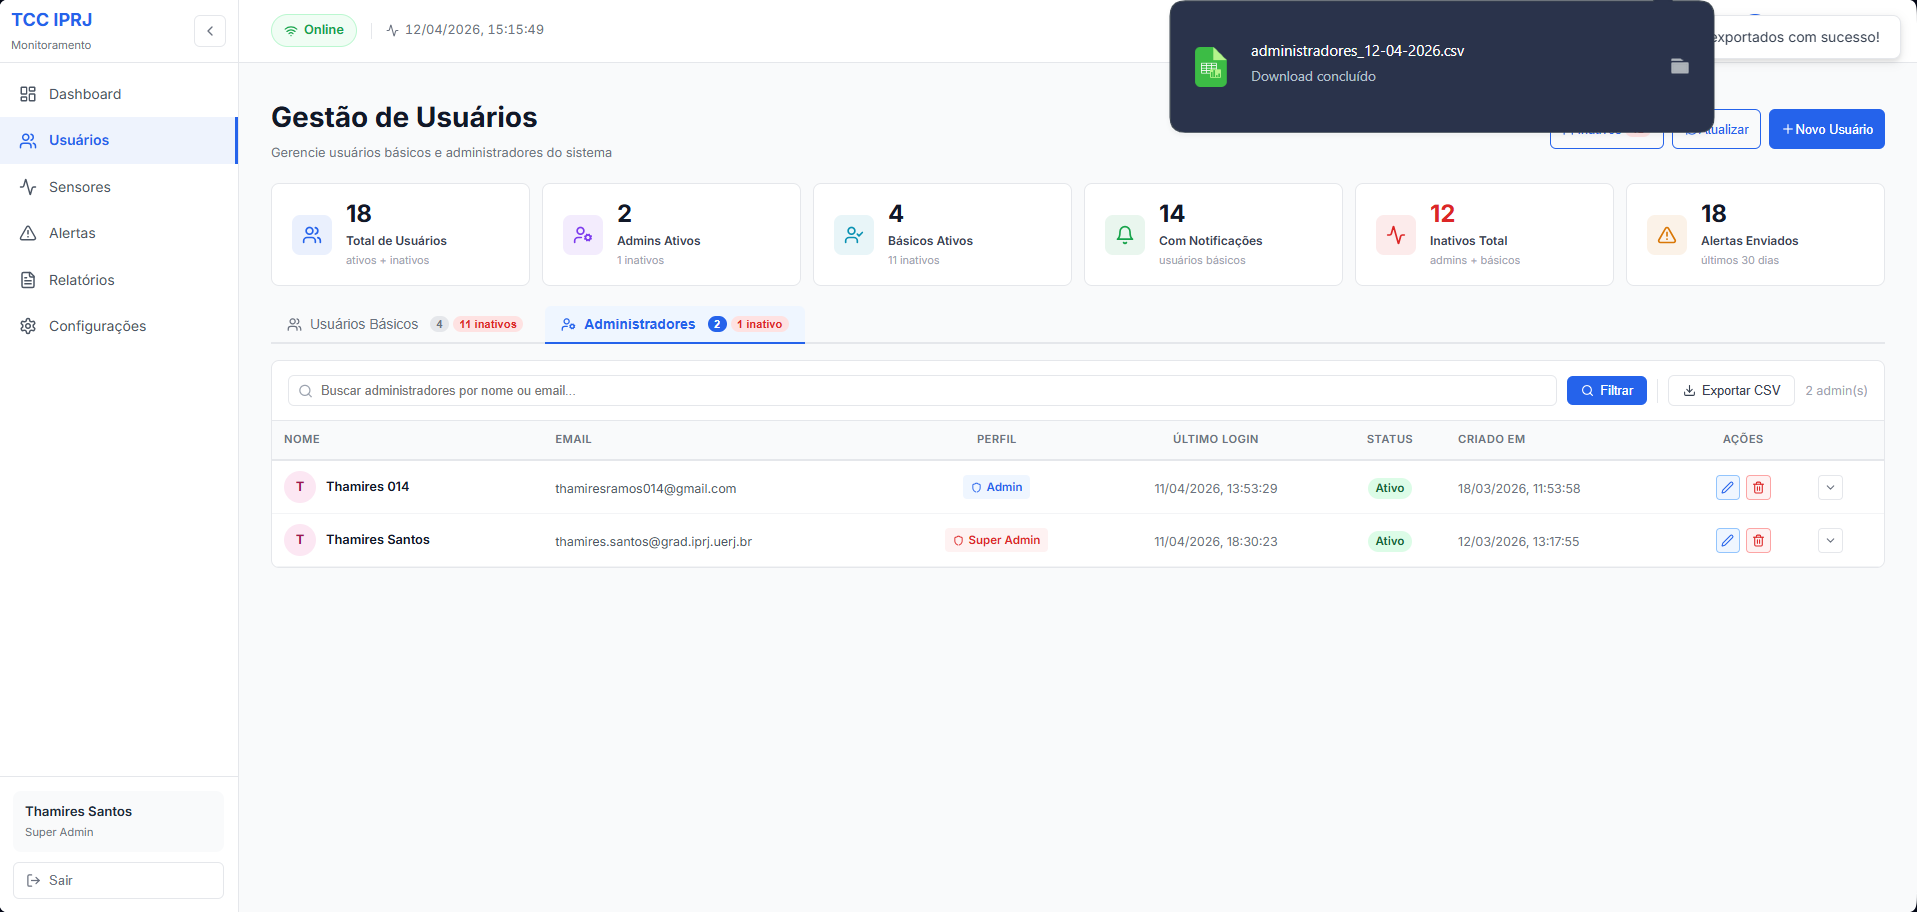
\includegraphics[width=0.95\textwidth]{figures/cap5_usuarios_csv_sucesso.png}
    \caption{Tela de Gestão de Usuários com \textit{toast} ``X registros exportados com sucesso'' ao gerar CSV com registros disponíveis na aba ativa.}
    \label{fig:usuarios_csv_sucesso}
    \fonte{Elaborado pela autora.}
\end{figure}

\begin{figure}[htbp]
    \centering
    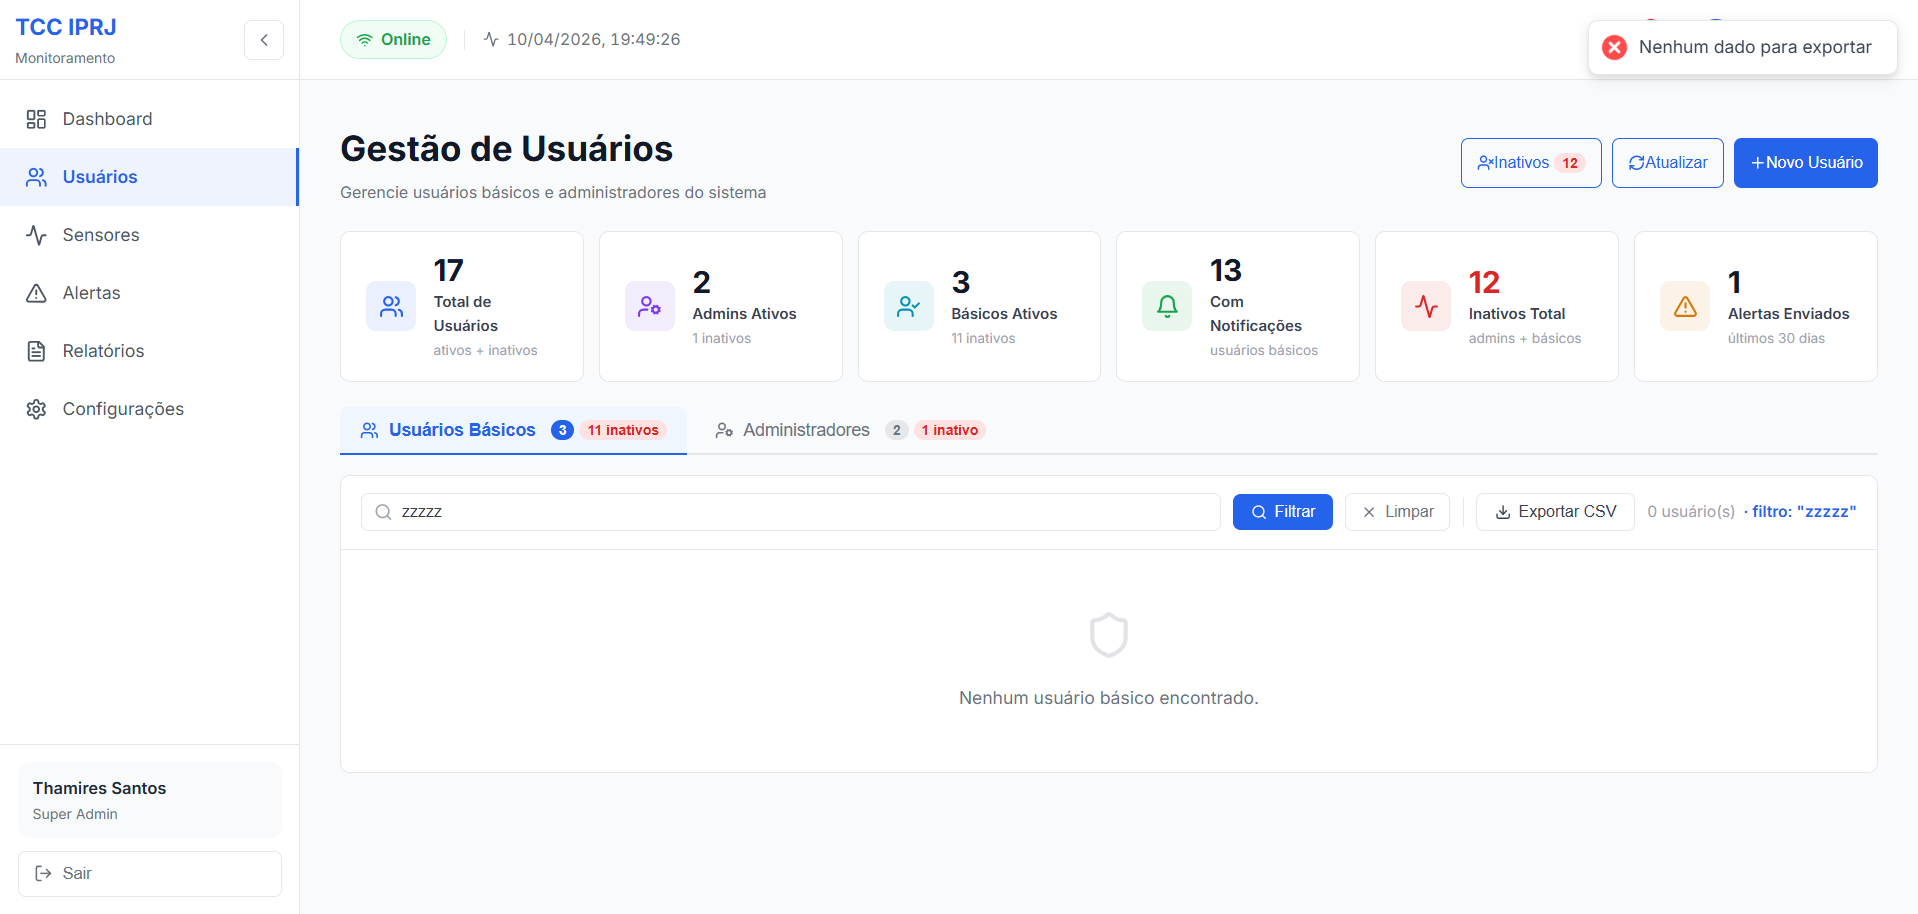
\includegraphics[width=0.95\textwidth]{figures/cap5_usuarios_csv_sem_dados.png}
    \caption{Tela de Gestão de Usuários com \textit{toast} ``Nenhum dado para exportar'' ao tentar gerar CSV sem registros disponíveis na aba ativa.}
    \label{fig:usuarios_csv_sem_dados}
    \fonte{Elaborado pela autora.}
\end{figure}

Falhas de comunicação com o \textit{backend} durante a exportação produzem um erro distinto, conforme ilustra a \autoref{fig:usuarios_csv_erro_backend}.

\begin{figure}[htbp]
    \centering
    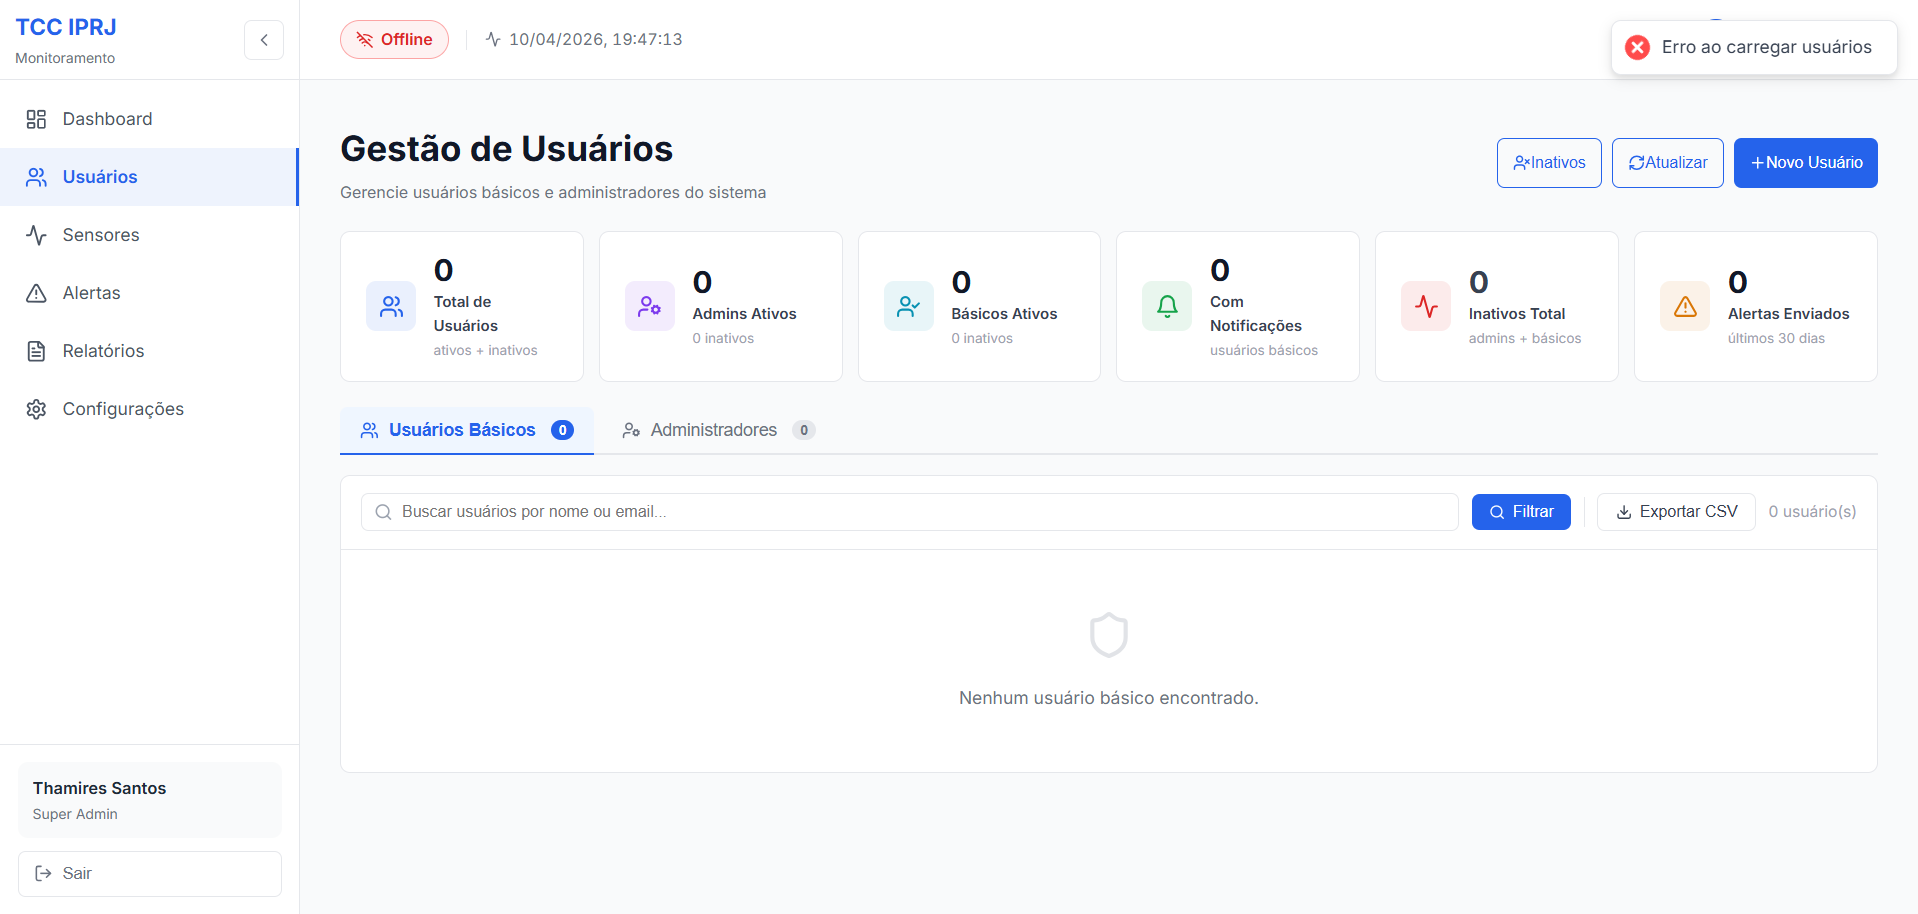
\includegraphics[width=0.95\textwidth]{figures/cap5_usuarios_csv_erro_backend.png}
    \caption{Tela de Gestão de Usuários com \textit{toast} ``Erro ao carregar usuários'': falha na requisição ao \textit{backend} durante a geração do arquivo CSV.}
    \label{fig:usuarios_csv_erro_backend}
    \fonte{Elaborado pela autora.}
\end{figure}

% -------------------------------------------------------------
\subsection{Gerenciamento de Administradores e Cadastro}
\label{subsec:admins}
% -------------------------------------------------------------

A aba ``Administradores'', exibe a
tabela de contas com o último \textit{login} de cada uma, os botões de
editar e desativar por linha, exclusiva ao \textit{super\_admin}, e o botão ``Novo Usuário'' para cadastrar
um novo administrador. A \autoref{fig:usuarios_admins} ilustra essa tela.

\begin{figure}[htbp]
    \centering
    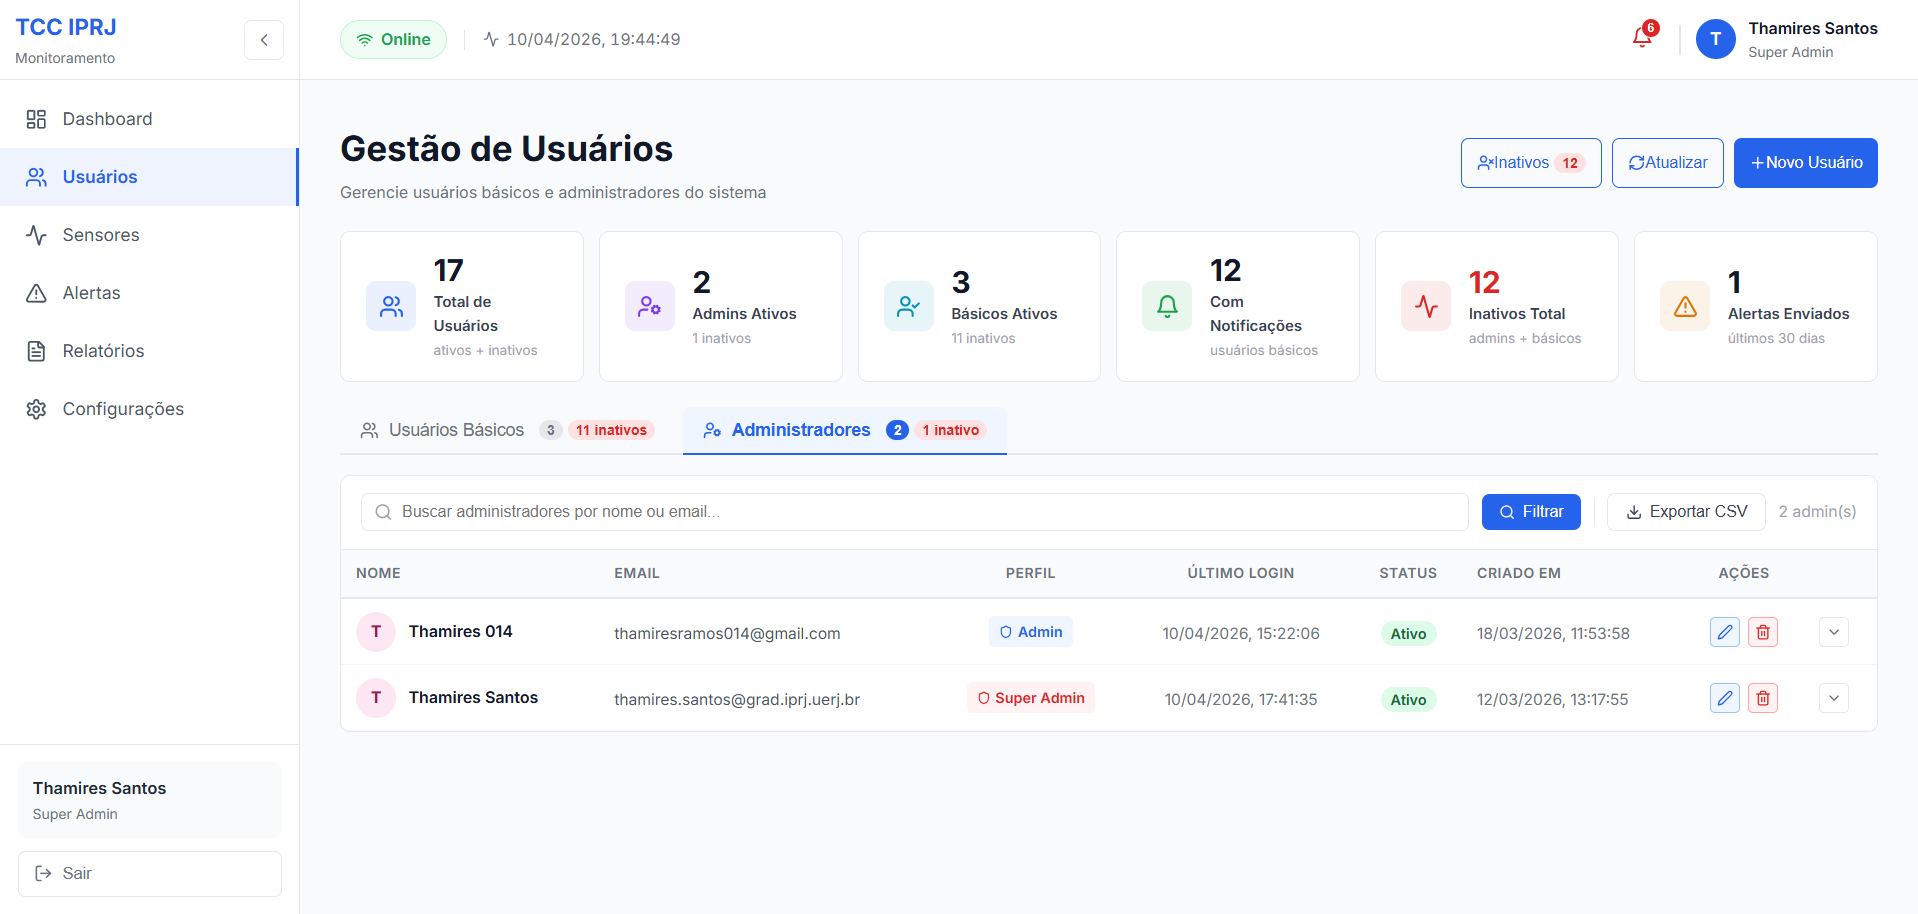
\includegraphics[width=0.95\textwidth]{figures/cap5_usuarios_admins.png}
    \caption{Tela de Gestão de Usuários com aba ``Administradores'' ativa
    (perfil \textit{super\_admin}): tabela com último \textit{login}
    e botões de editar e desativar por linha.}
    \label{fig:usuarios_admins}
    \fonte{Elaborado pela autora.}
\end{figure}

O formulário de cadastro de administrador inclui o campo de perfil, onde
se define se o novo usuário terá acesso de administrador padrão ou de
\textit{super\_admin}. Senhas que não atendam ao critério mínimo são
recusadas com mensagem de erro antes do envio ao servidor, conforme ilustra a \autoref{fig:admin_form_senha_invalida}.

\begin{figure}[htbp]
    \centering
    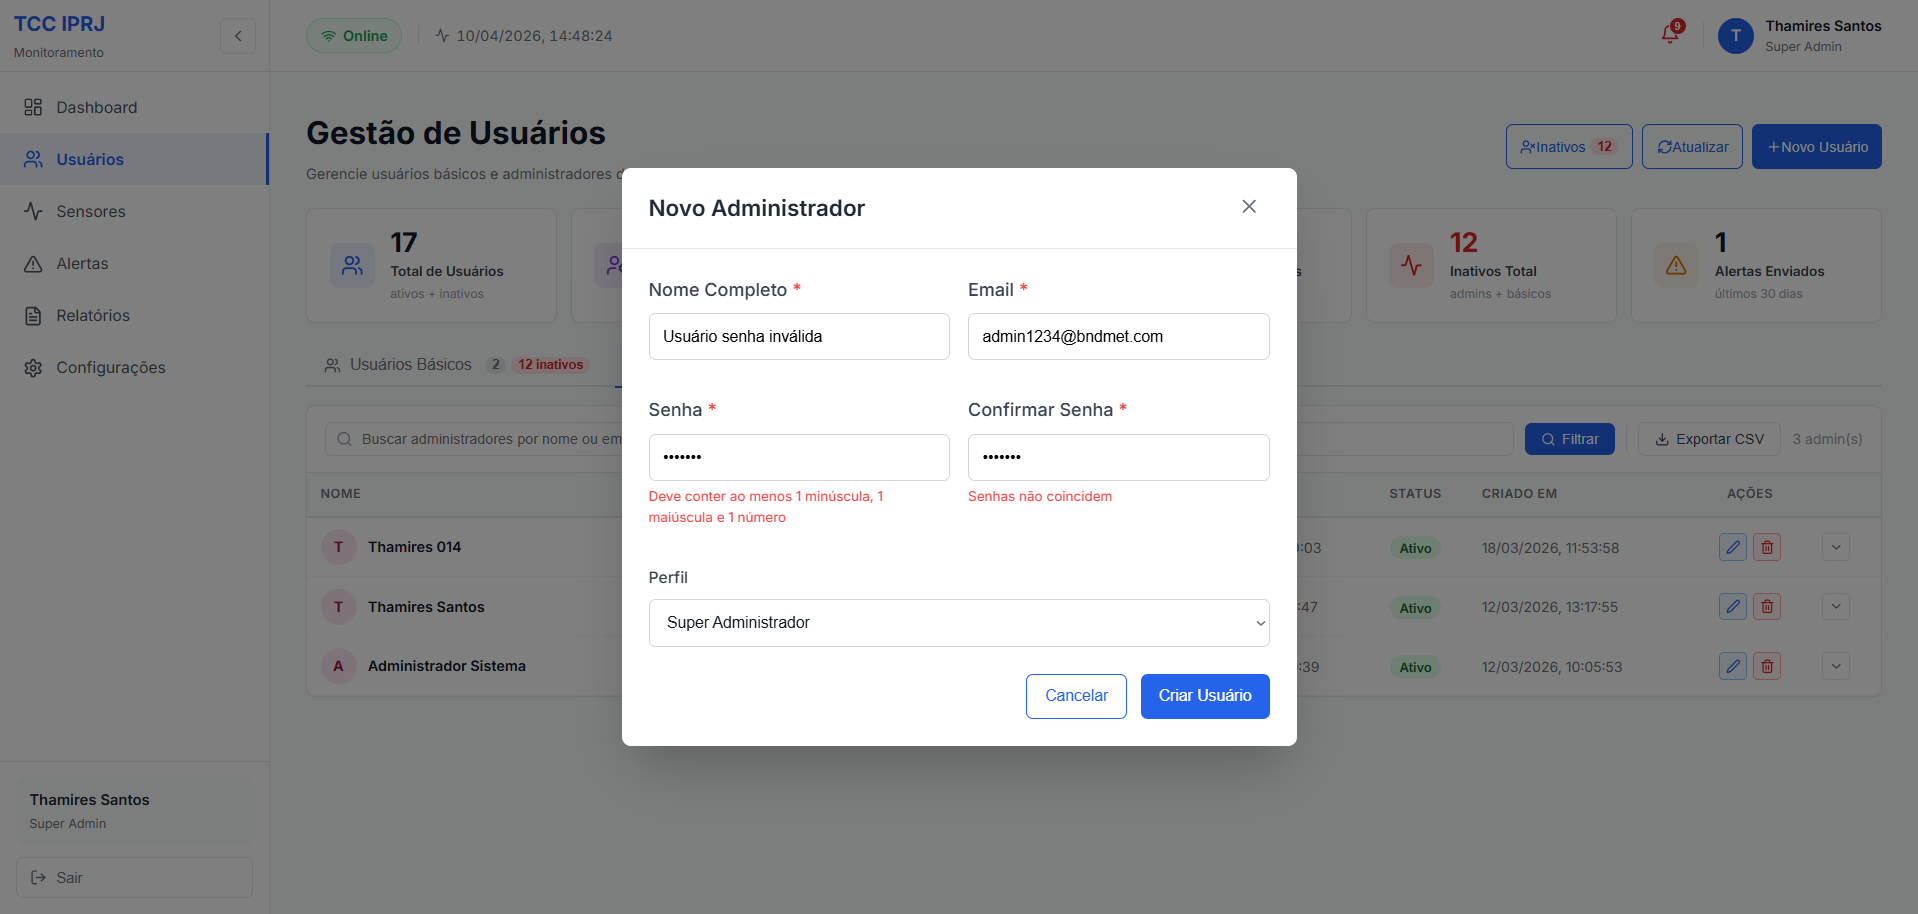
\includegraphics[width=0.75\textwidth]{figures/cap5_admin_form_senha_invalida.png}
    \caption{Formulário de cadastro de administrador com senha inválida: mensagem de erro inline antes do envio; botão ``Criar Usuário'' permanece habilitado para nova tentativa.}
    \label{fig:admin_form_senha_invalida}
    \fonte{Elaborado pela autora.}
\end{figure}

E-mails duplicados também geram erro com mensagem de retorno, conforme ilustra a \autoref{fig:admin_form_email_duplicado}.

\begin{figure}[htbp]
    \centering
    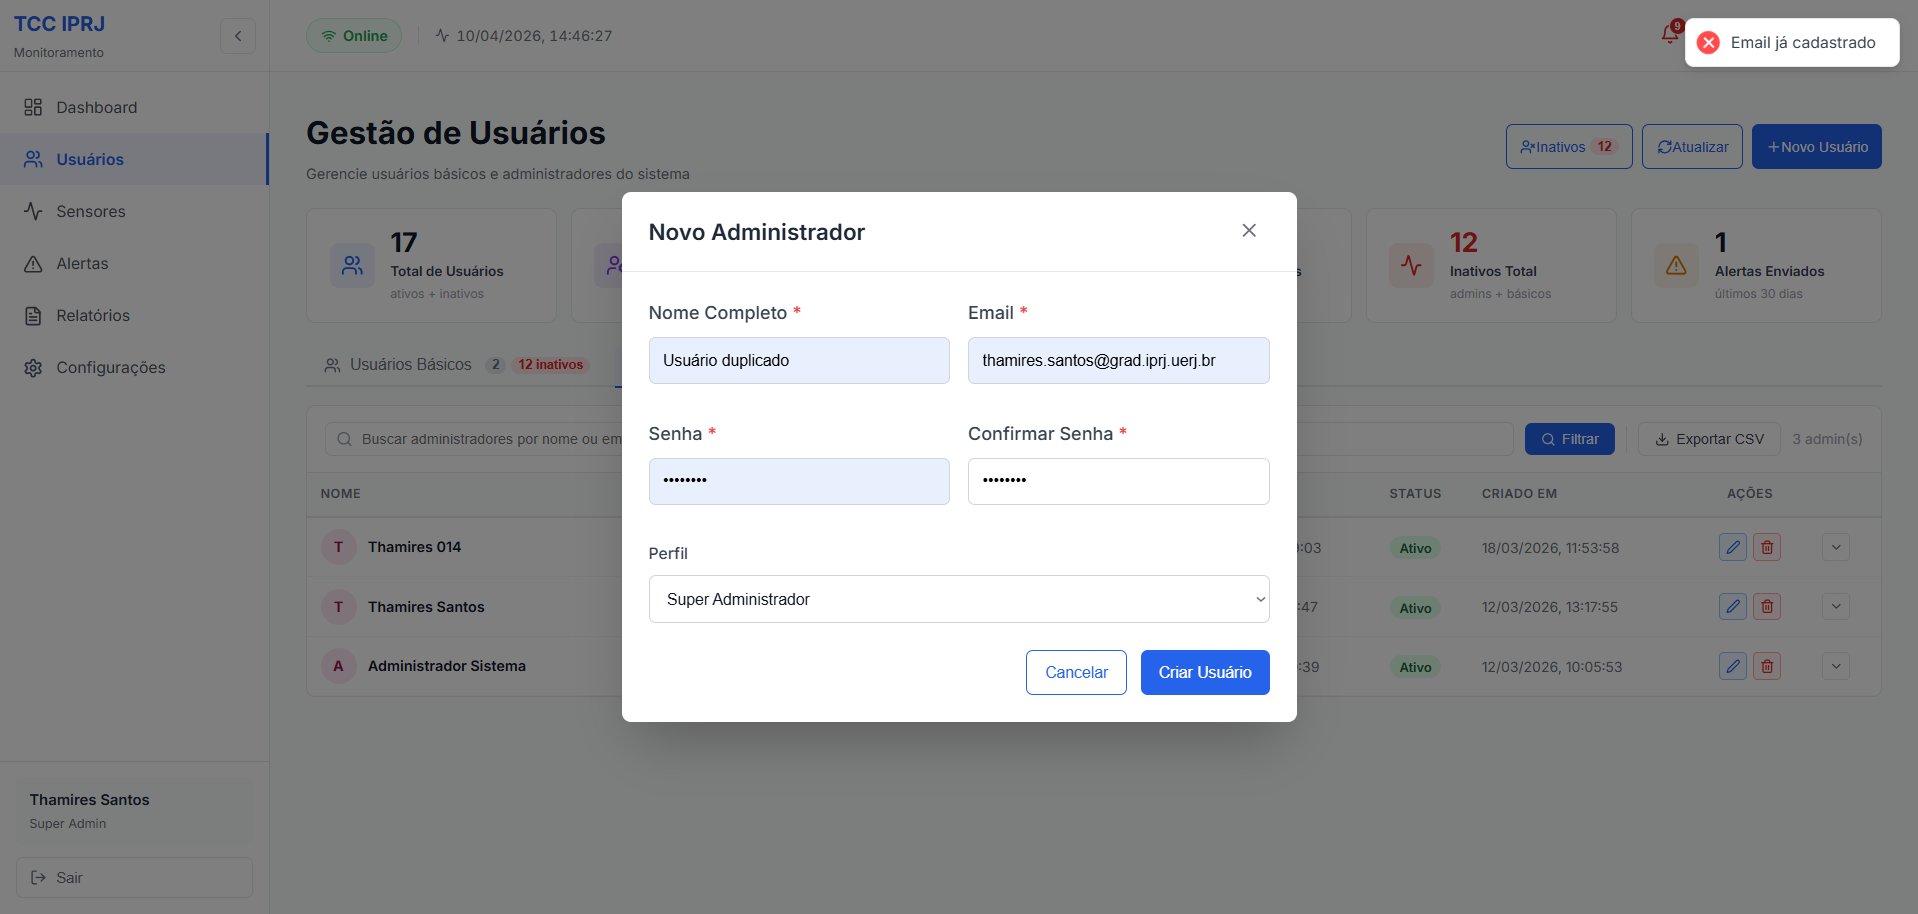
\includegraphics[width=0.75\textwidth]{figures/cap5_admin_form_email_duplicado.png}
    \caption{Formulário de cadastro de administrador com \textit{toast} de e-mail duplicado: \textit{backend} retorna HTTP 400 ``Email já cadastrado''; formulário retorna para correção do dado.}
    \label{fig:admin_form_email_duplicado}
    \fonte{Elaborado pela autora.}
\end{figure}

Tentativas de
criação de administradores por contas sem perfil \textit{super\_admin}
são bloqueadas pelo \textit{middleware} do \textit{backend}, que retorna
HTTP~403 ``Acesso negado'', que resulta nos botões de editar e desativar desabilitados na tabela, conforme ilustra a \autoref{fig:admins_sem_permissao}.

\begin{figure}[htbp]
    \centering
    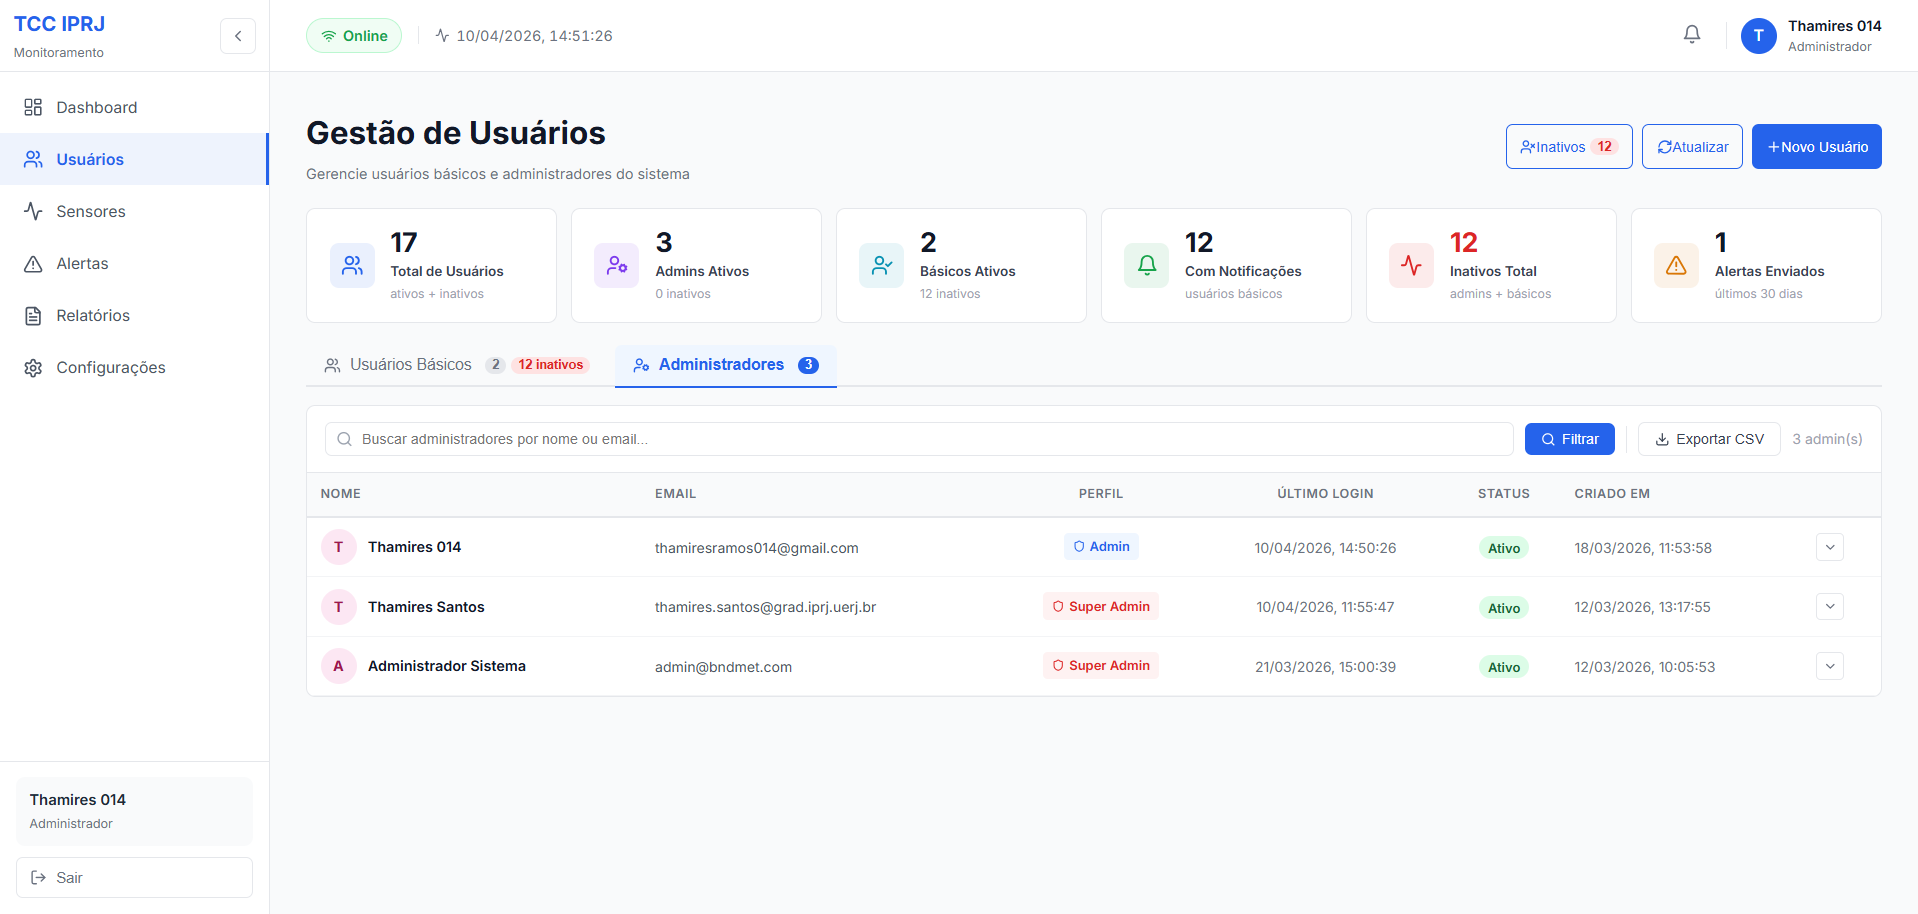
\includegraphics[width=0.95\textwidth]{figures/cap5_admins_sem_permissao.png}
    \caption{Aba ``Administradores'' acessada por conta sem perfil \textit{super\_admin}: botões de editar e desativar desabilitados na tabela.}
    \label{fig:admins_sem_permissao}
    \fonte{Elaborado pela autora.}
\end{figure}

% =============================================================
\section{Configurações do Sistema}
\label{sec:configuracoes}
% =============================================================

% -------------------------------------------------------------
\subsection{Atualização de Perfil}
\label{subsec:config-perfil}
% -------------------------------------------------------------

A tela de Configurações (\autoref{fig:configuracoes}) apresenta o
formulário de atualização de dados de conta com os campos nome e e-mail
pré-preenchidos, além de informações de sessão em modo leitura --- perfil
de acesso, identificador único e dados do último acesso. Após alterar
os campos e clicar em ``Salvar Alterações'', o \textit{toast} ``Perfil
atualizado com sucesso!'' confirma a operação e o nome exibido no
cabeçalho da aplicação é atualizado sem necessidade de novo \textit{login}, conforme mostra a \autoref{fig:configuracoes_edicao}.
Quando o e-mail já é utilizado por outro administrador, o \textit{backend}
retorna erro e o sistema exibe a mensagem ``Este email já está em uso
por outro usuário'', conforme ilustra a \autoref{fig:config_email_em_uso}.

\begin{figure}[htbp]
    \centering
    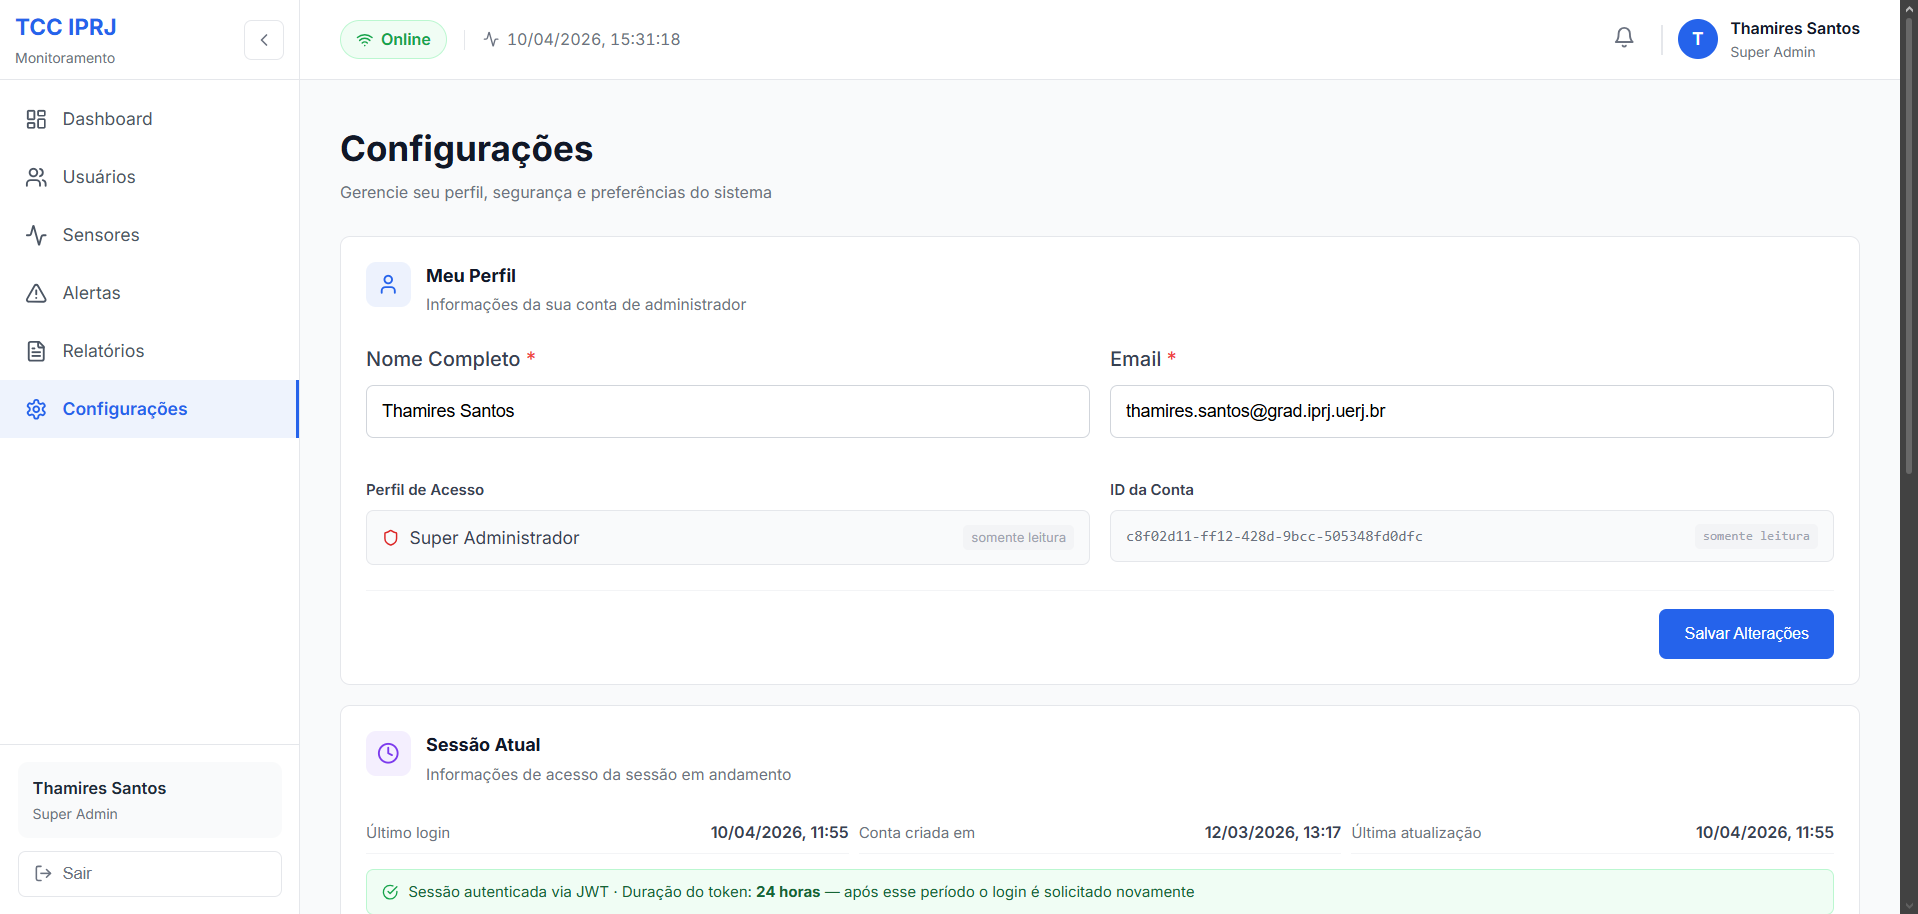
\includegraphics[width=0.95\textwidth]{figures/cap5_configuracoes.png}
    \caption{Tela de Configurações: formulário de atualização de nome e
    e-mail com informações de sessão em modo leitura.}
    \label{fig:configuracoes}
    \fonte{Elaborado pela autora.}
\end{figure}

\begin{figure}[htbp]
    \centering
    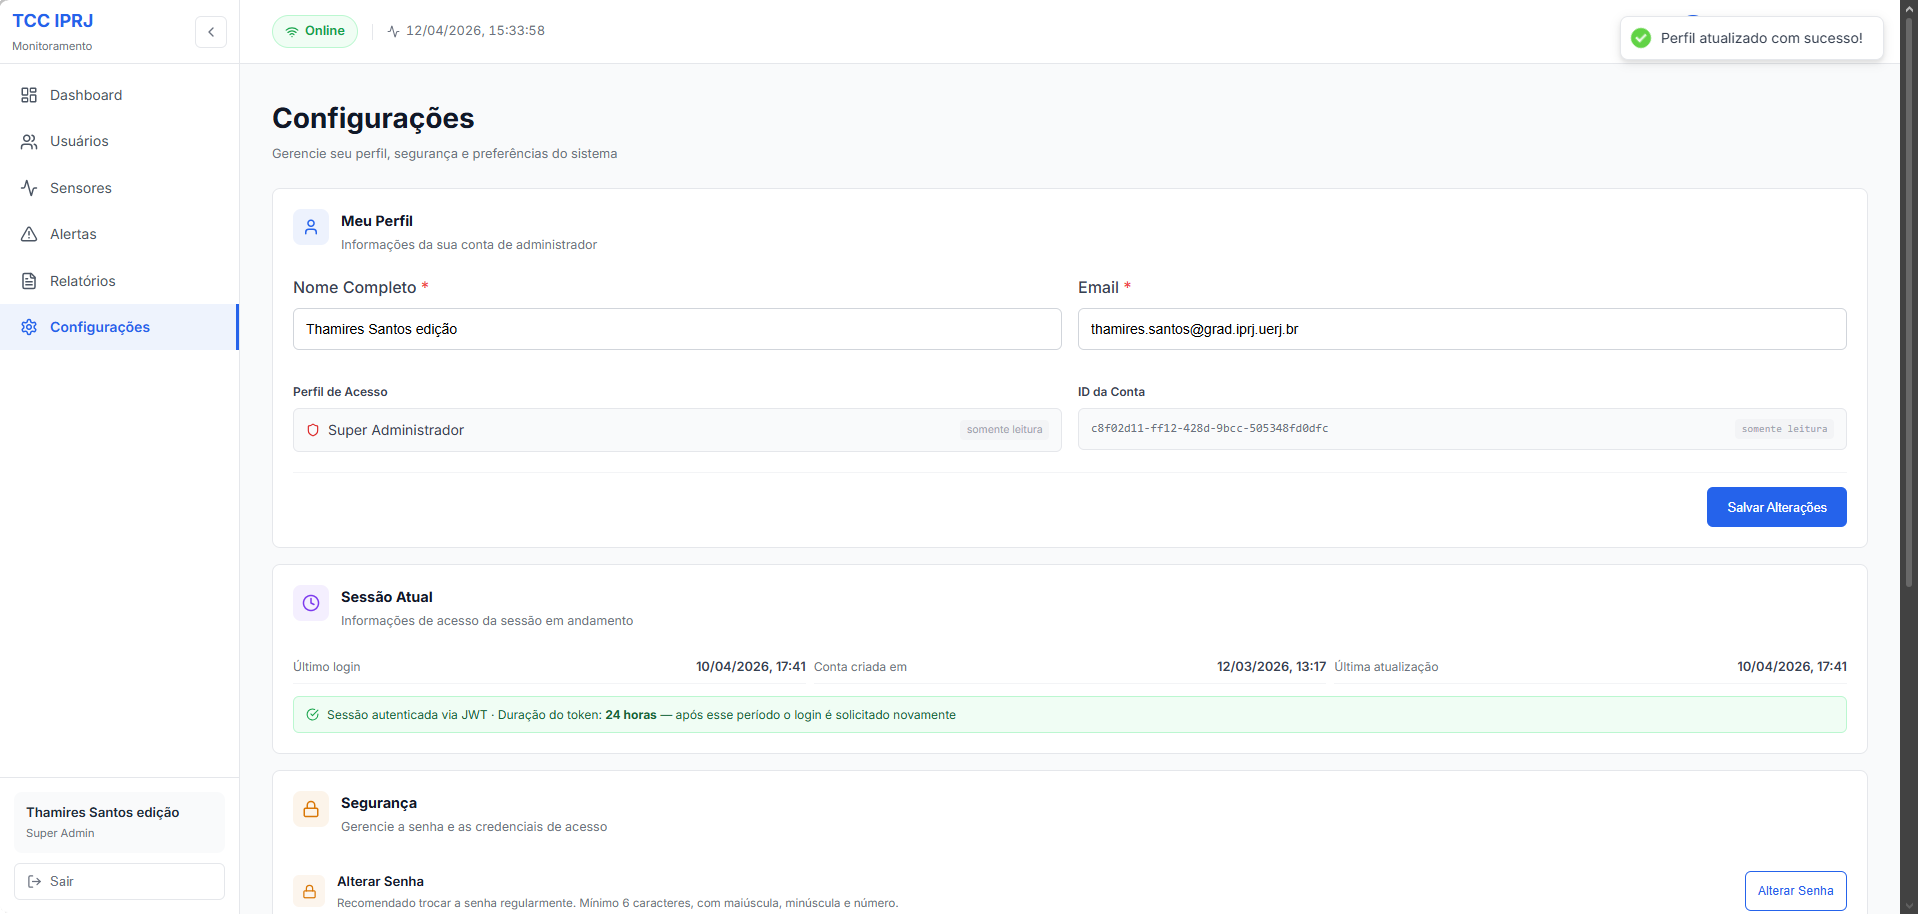
\includegraphics[width=0.95\textwidth]{figures/cap5_configuracoes_edicao.png}
    \caption{Tela de Configurações: \textit{toast} ``Perfil atualizado com sucesso!'' e dado atualizado sem necessidade de novo \textit{login}.}
    \label{fig:configuracoes_edicao}
    \fonte{Elaborado pela autora.}
\end{figure}

\begin{figure}[htbp]
    \centering
    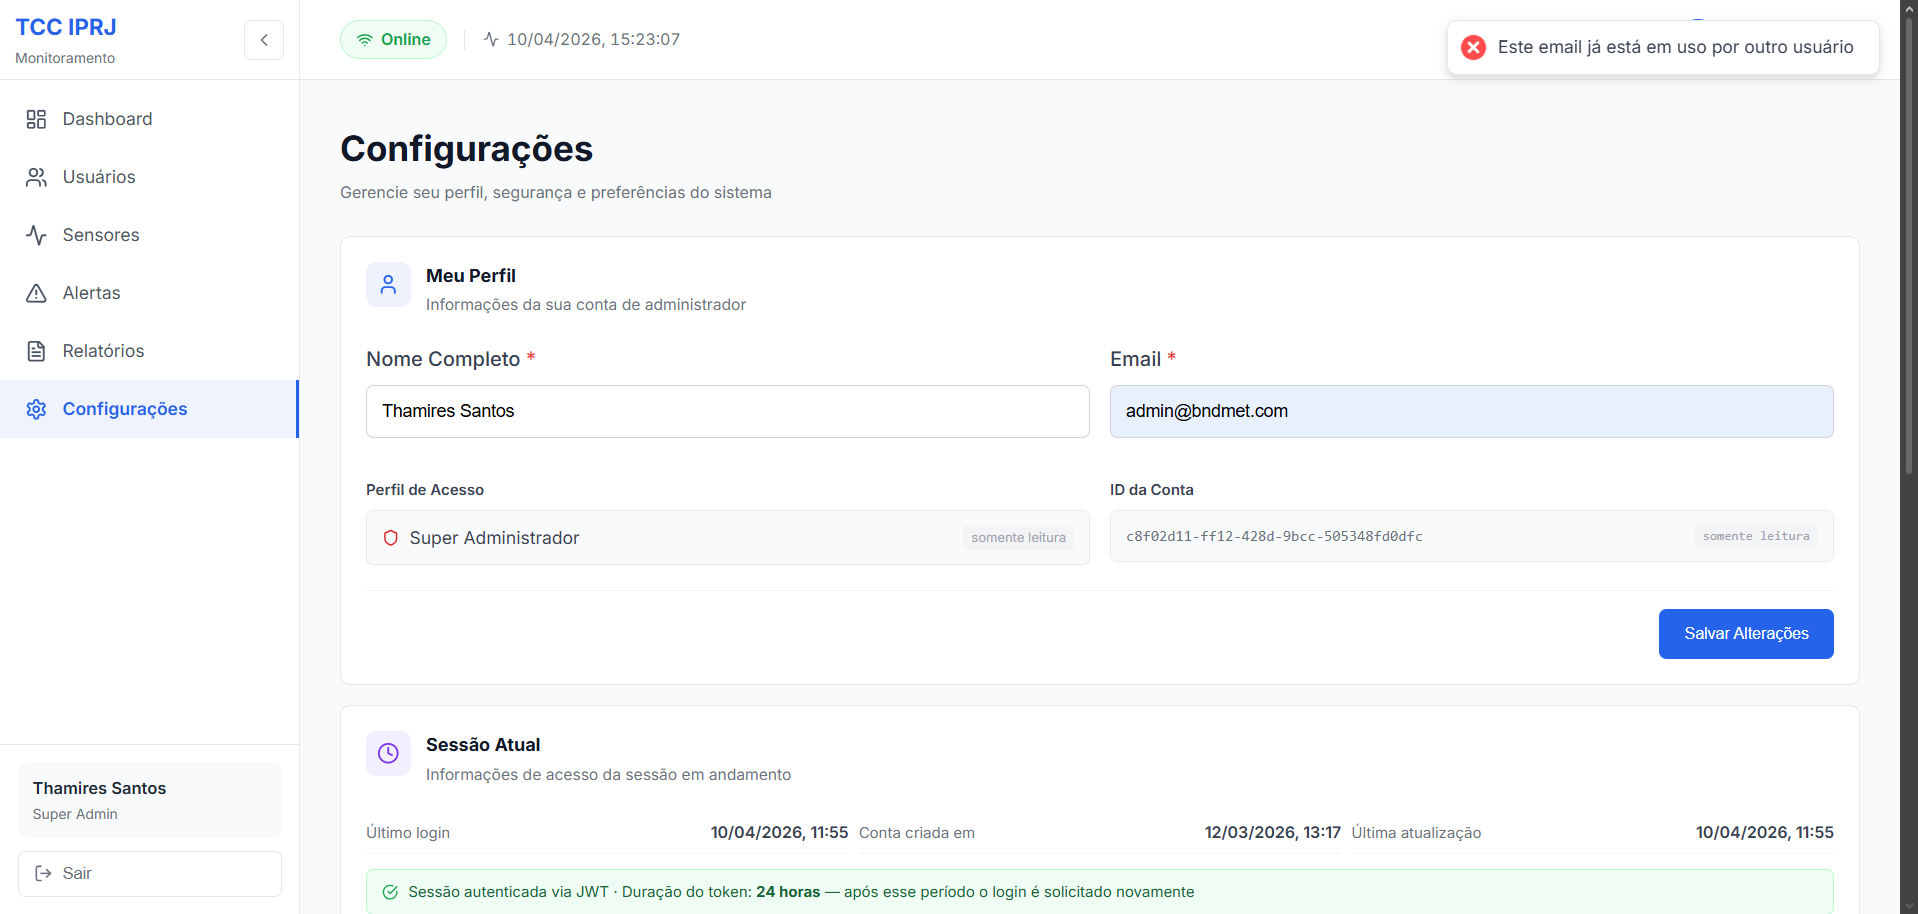
\includegraphics[width=0.95\textwidth]{figures/cap5_config_email_em_uso.png}
    \caption{Tela de Configurações com \textit{toast} de conflito de e-mail: endereço informado já utilizado por outro administrador; campo retorna para correção.}
    \label{fig:config_email_em_uso}
    \fonte{Elaborado pela autora.}
\end{figure}

Para o perfil \textit{super\_admin}, a tela exibe seção adicional.
A seção, ``Informações
Técnicas'', apresenta dados em tempo real obtidos do \textit{backend}:
status geral, versão da API, ambiente de operação, \textit{uptime} do
processo, status e latência do banco de dados, status e último contato
do sensor ESP8266, memória utilizada e nível de alerta atual com
confiabilidade, como mostra a \autoref{fig:configuracoes_superadmin}.
Quando os dados técnicos não podem ser carregados, a seção exibe um
estado de erro com botão ``Tentar novamente'', conforme ilustra a \autoref{fig:config_health_erro}.

\begin{figure}[htbp]
    \centering
    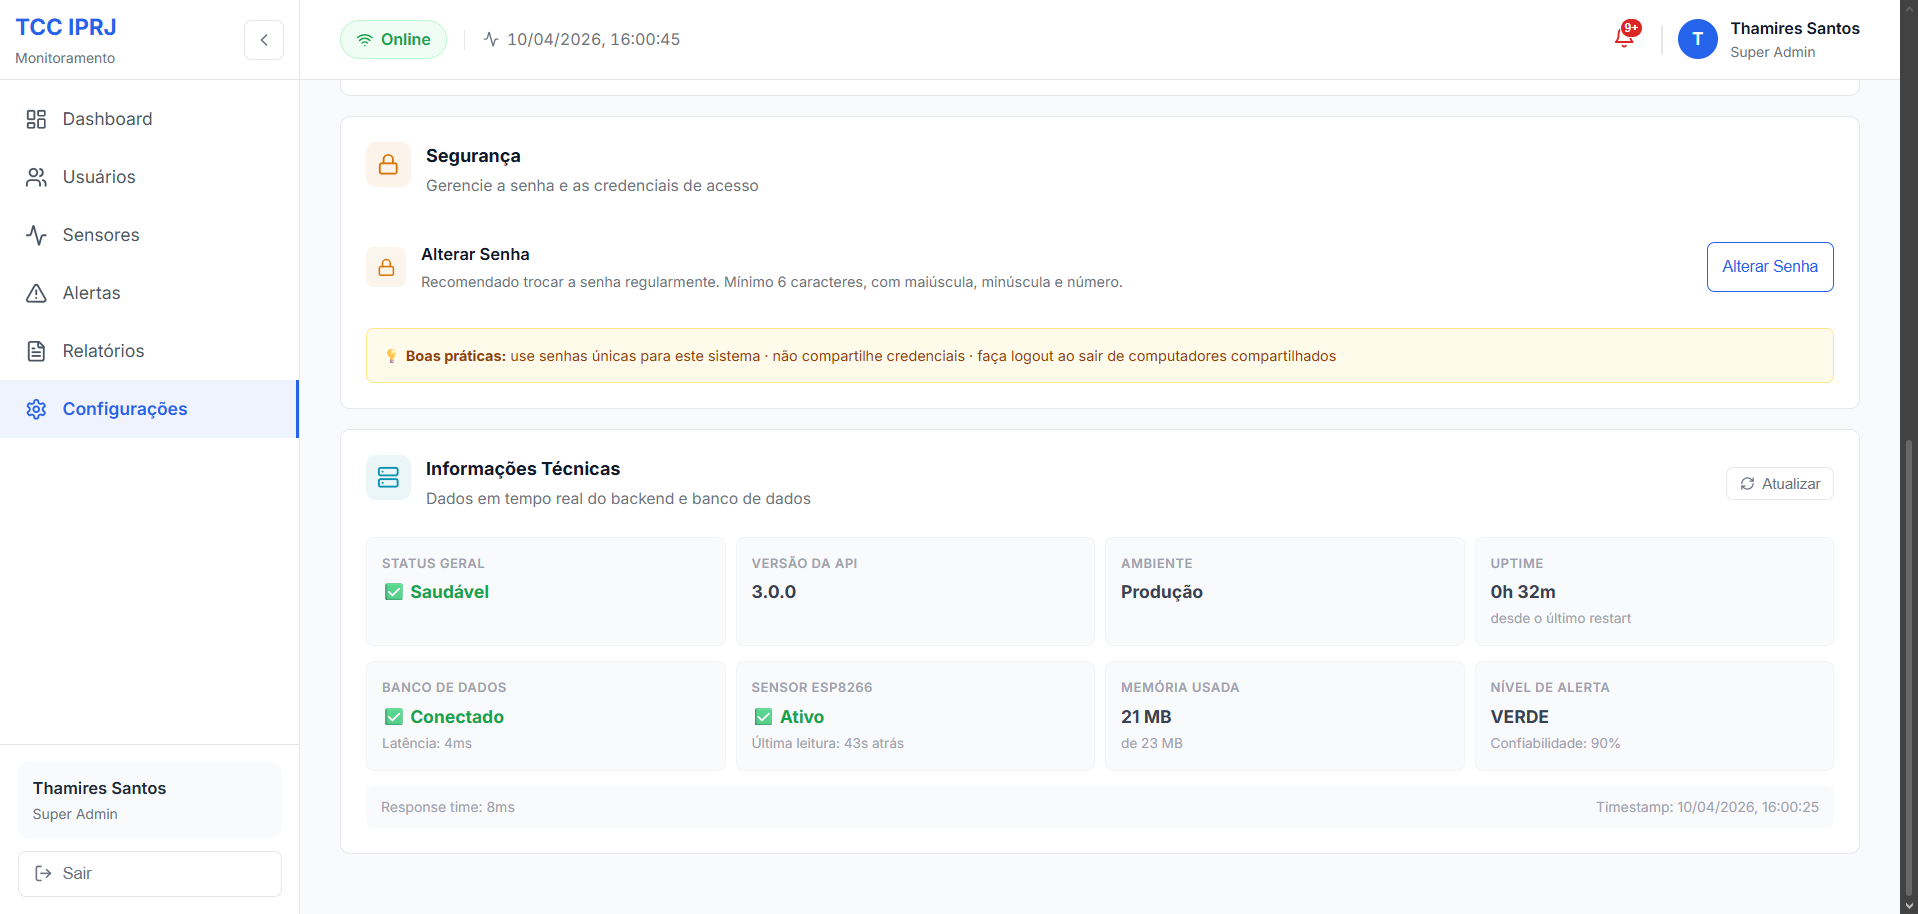
\includegraphics[width=0.95\textwidth]{figures/cap5_configuracoes_superadmin.png}
    \caption{Tela de Configurações com seção exclusiva ao
    \textit{super\_admin}: Informações Técnicas em tempo real.}
    \label{fig:configuracoes_superadmin}
    \fonte{Elaborado pela autora.}
\end{figure}

\begin{figure}[htbp]
    \centering
    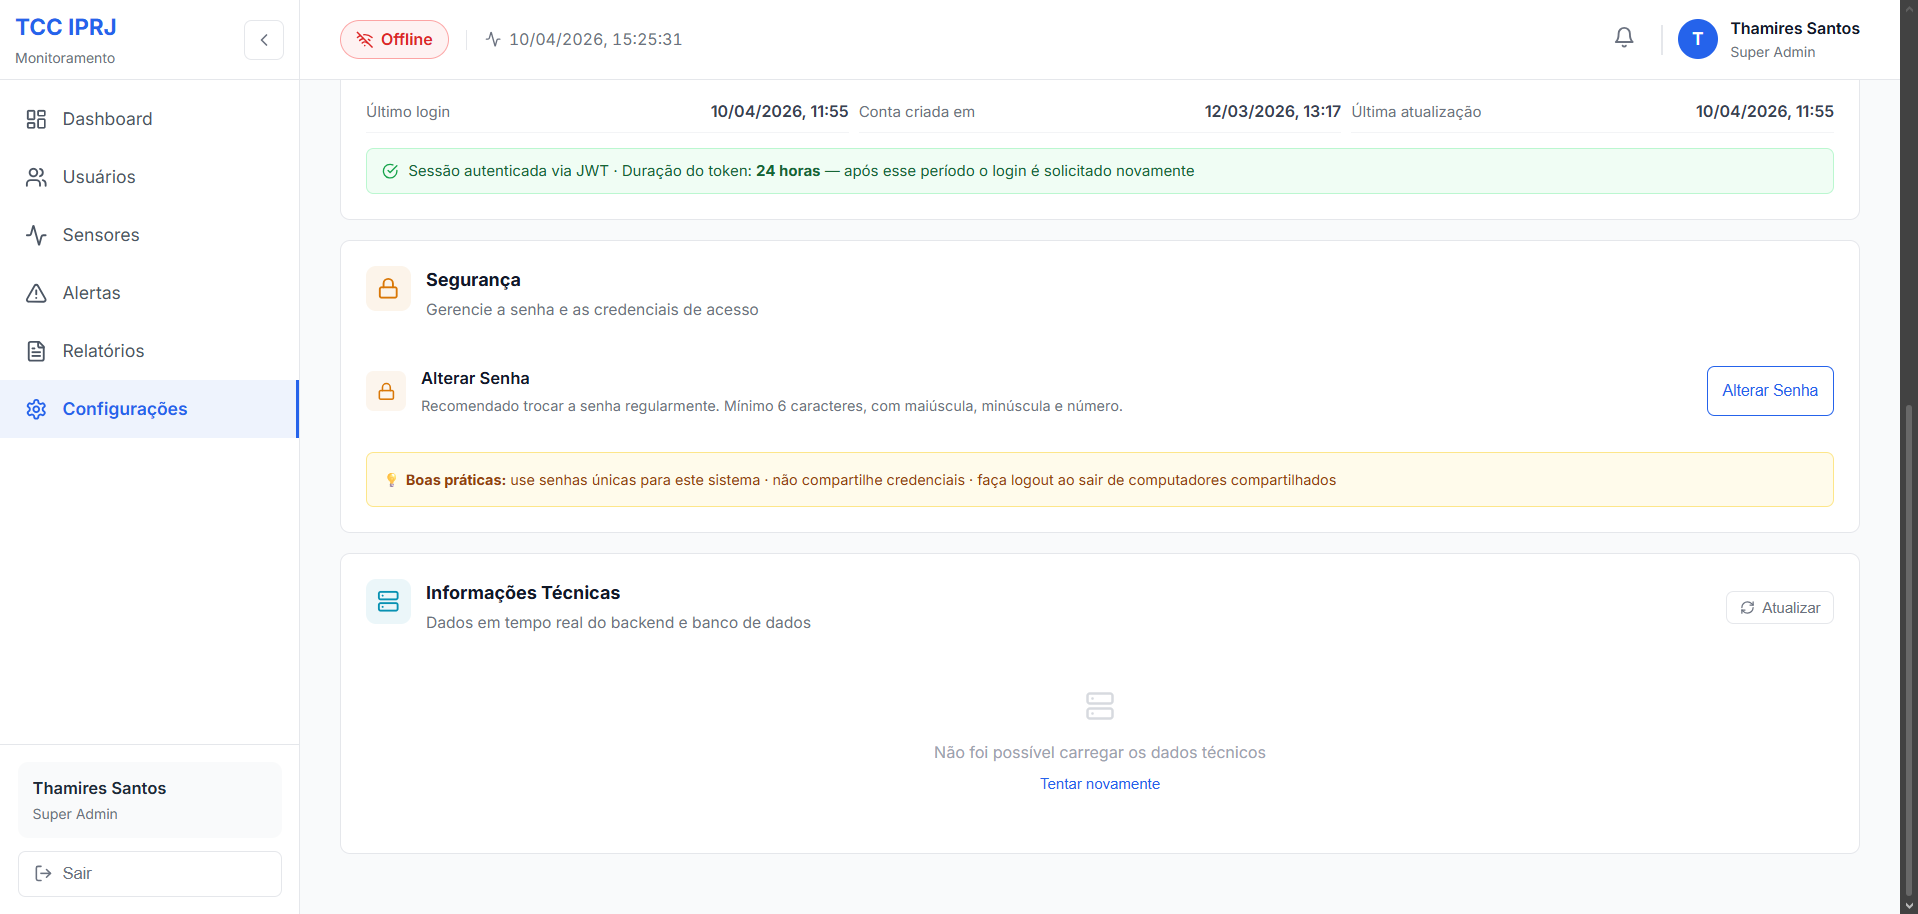
\includegraphics[width=0.95\textwidth]{figures/cap5_config_health_erro.png}
    \caption{Seção ``Informações Técnicas'' na tela de Configurações com estado de erro: dados de saúde do \textit{backend} inacessíveis e botão ``Tentar novamente'' disponível para nova tentativa.}
    \label{fig:config_health_erro}
    \fonte{Elaborado pela autora.}
\end{figure}

% -------------------------------------------------------------
\subsection{Alteração de Senha}
\label{subsec:config-senha}
% -------------------------------------------------------------

O botão ``Alterar Senha'' abre um modal com três campos: senha atual,
nova senha e confirmação. A nova senha deve conter ao menos 6 caracteres,
com pelo menos uma letra maiúscula, uma minúscula e um número; senhas
fora desse padrão geram mensagem de erro inline antes do envio. Após
a confirmação bem-sucedida, todas as sessões ativas do administrador
são invalidadas, o \textit{toast} ``Senha alterada com sucesso!'' é
exibido e o modal é fechado. As \autoref{fig:alterar_senha_modal_pt1} e
\autoref{fig:alterar_senha_modal_pt2} ilustram o modal com os campos
preenchidos.

\begin{figure}[htbp]
    \centering
    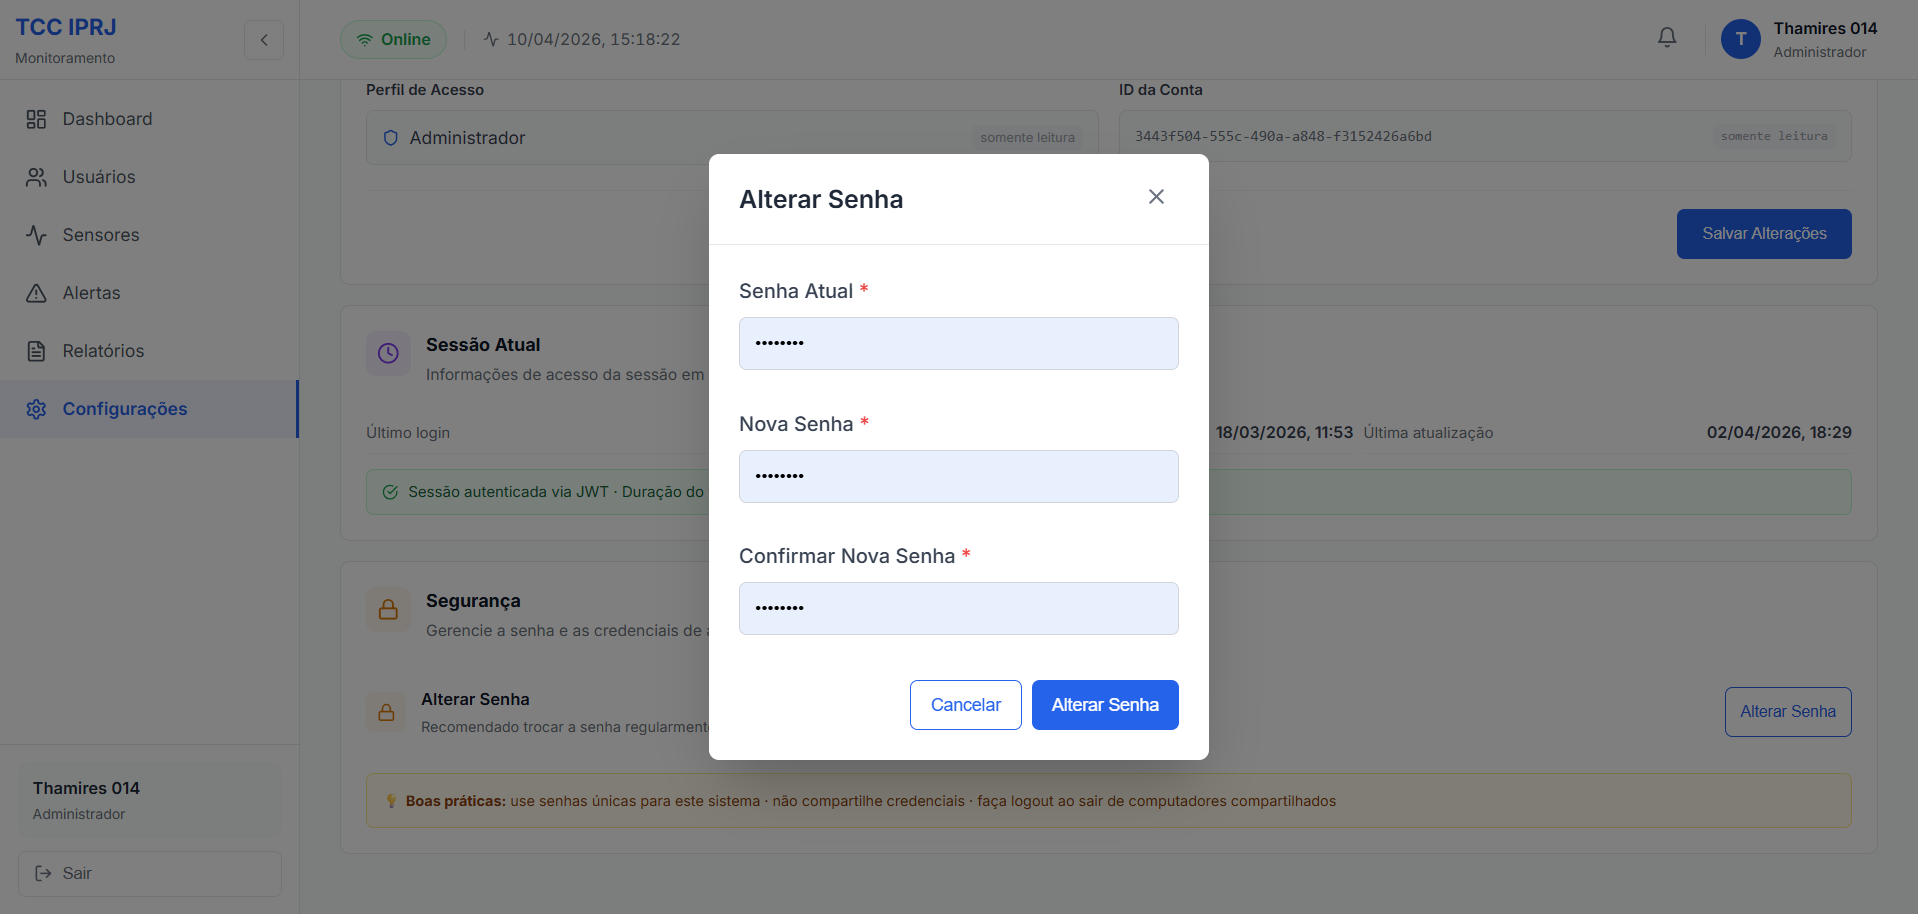
\includegraphics[width=0.75\textwidth]{figures/cap5_alterar_senha_modal_pt1.png}
    \caption{Modal de alteração de senha (parte~1): campos de senha atual
    e nova senha preenchidos; critérios de complexidade exigidos (mínimo
    de 6 caracteres com maiúscula, minúscula e número).}
    \label{fig:alterar_senha_modal_pt1}
    \fonte{Elaborado pela autora.}
\end{figure}

\begin{figure}[htbp]
    \centering
    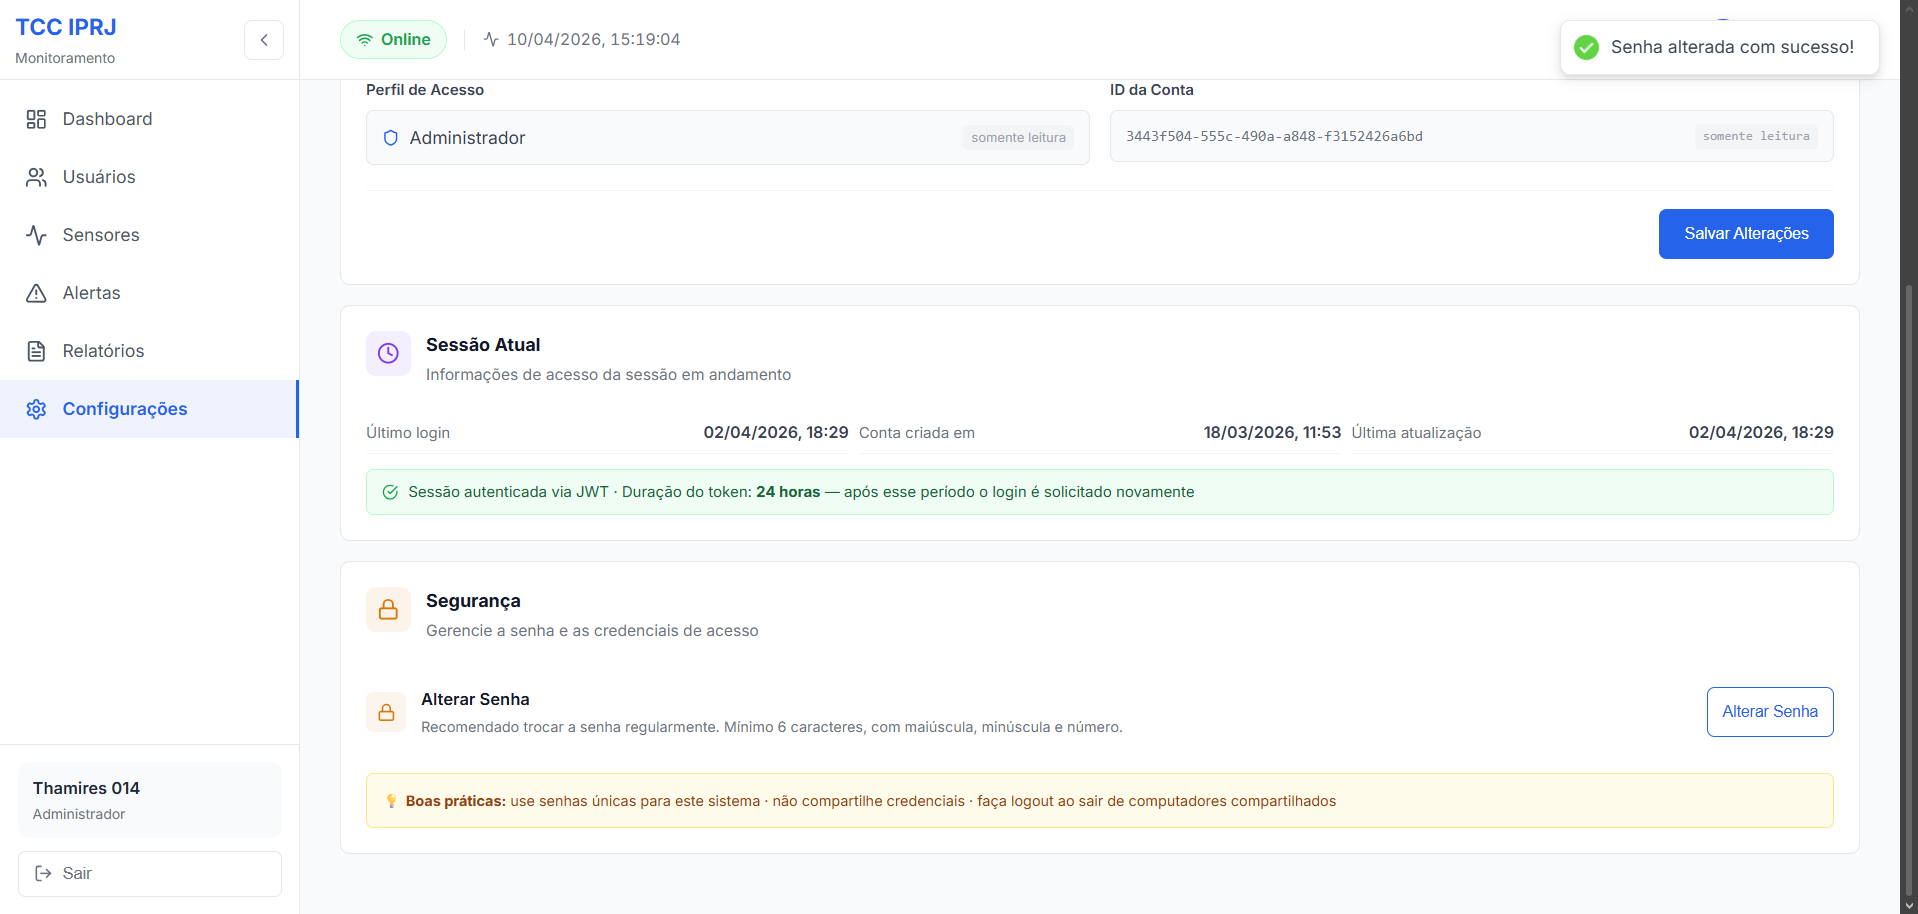
\includegraphics[width=0.75\textwidth]{figures/cap5_alterar_senha_modal_pt2.png}
    \caption{Modal de alteração de senha (parte~2): campo de confirmação
    de nova senha preenchido e botão ``Alterar Senha'' pronto para envio.}
    \label{fig:alterar_senha_modal_pt2}
    \fonte{Elaborado pela autora.}
\end{figure}

Quando a nova senha não atende aos critérios, a mensagem de erro é exibida inline antes do envio ao servidor, conforme ilustra a \autoref{fig:alterar_senha_nova_invalida}.

\begin{figure}[htbp]
    \centering
    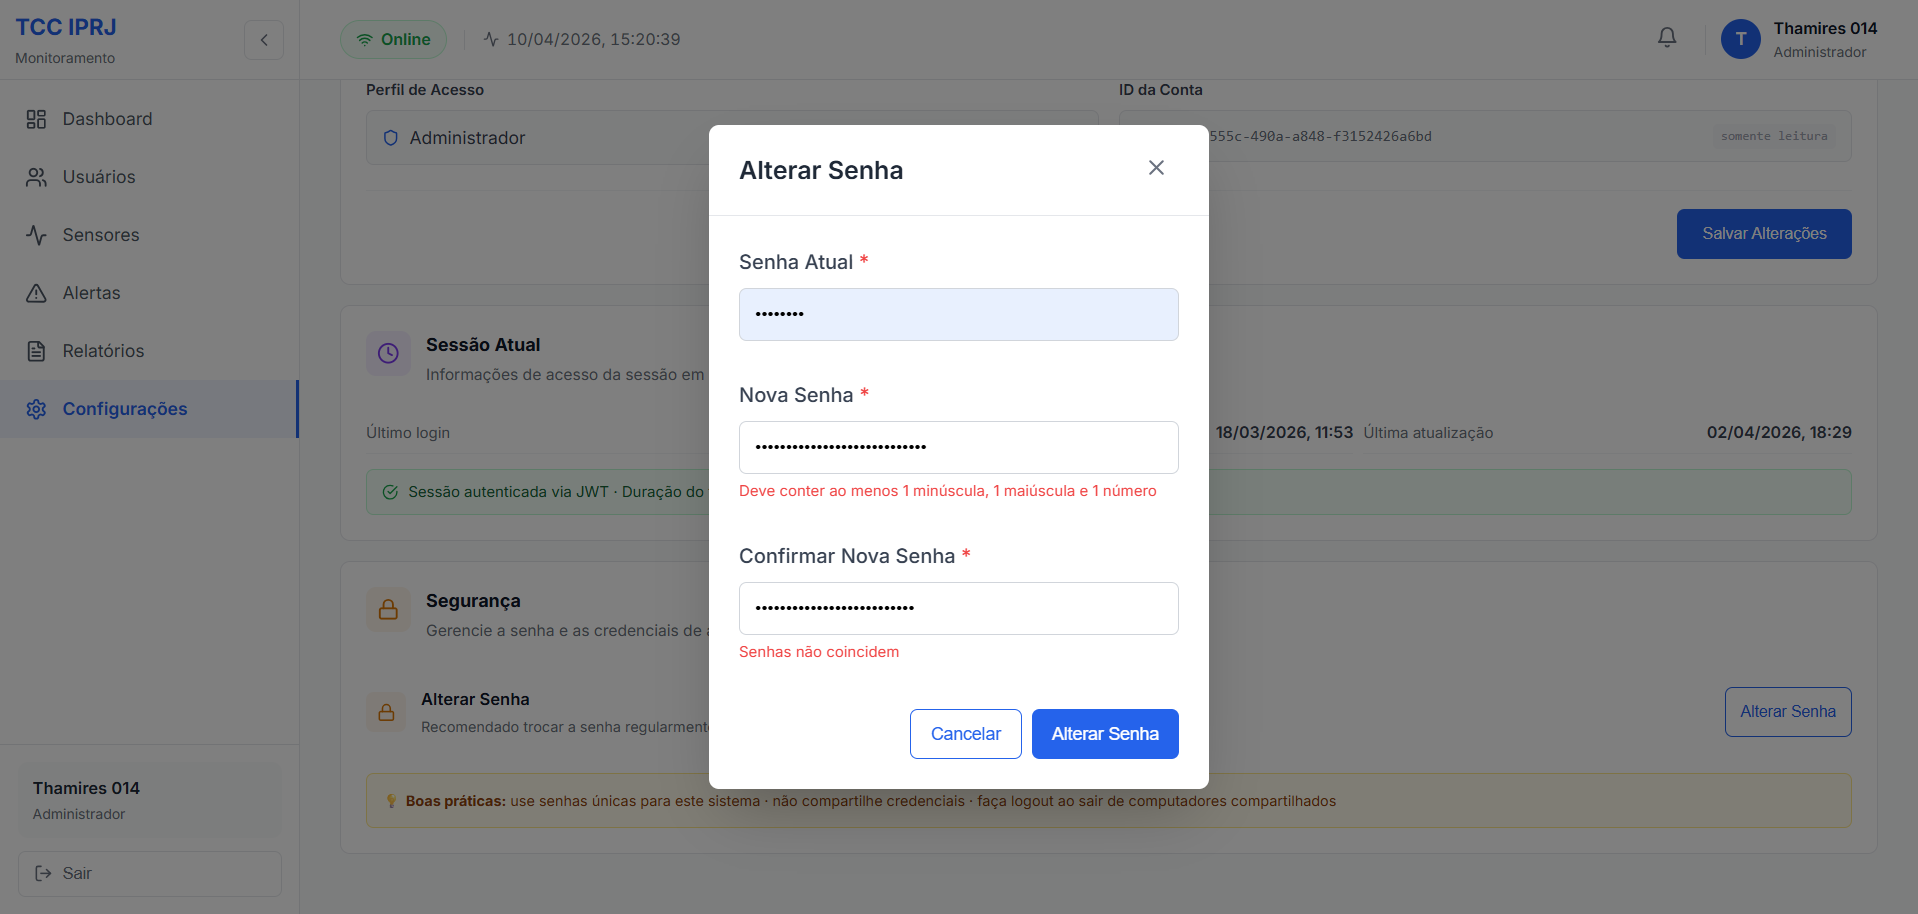
\includegraphics[width=0.75\textwidth]{figures/cap5_alterar_senha_nova_invalida.png}
    \caption{Modal de alteração de senha com mensagem de erro inline: nova senha fora dos critérios de complexidade; botão ``Alterar Senha'' permanece habilitado para nova tentativa.}
    \label{fig:alterar_senha_nova_invalida}
    \fonte{Elaborado pela autora.}
\end{figure}

A senha atual incorreta é detectada apenas no \textit{backend}, produzindo um \textit{toast} de erro distinto do erro inline: o \textit{backend} retorna HTTP~400 ``Senha atual incorreta'' e o formulário retorna para correção, conforme demonstra a \autoref{fig:alterar_senha_atual_incorreta}.

\begin{figure}[htbp]
    \centering
    \caption{Modal de alteração de senha com \textit{toast} de erro por senha atual incorreta: \textit{backend} retorna HTTP 400 ``Senha atual incorreta''; formulário retorna para correção.}
    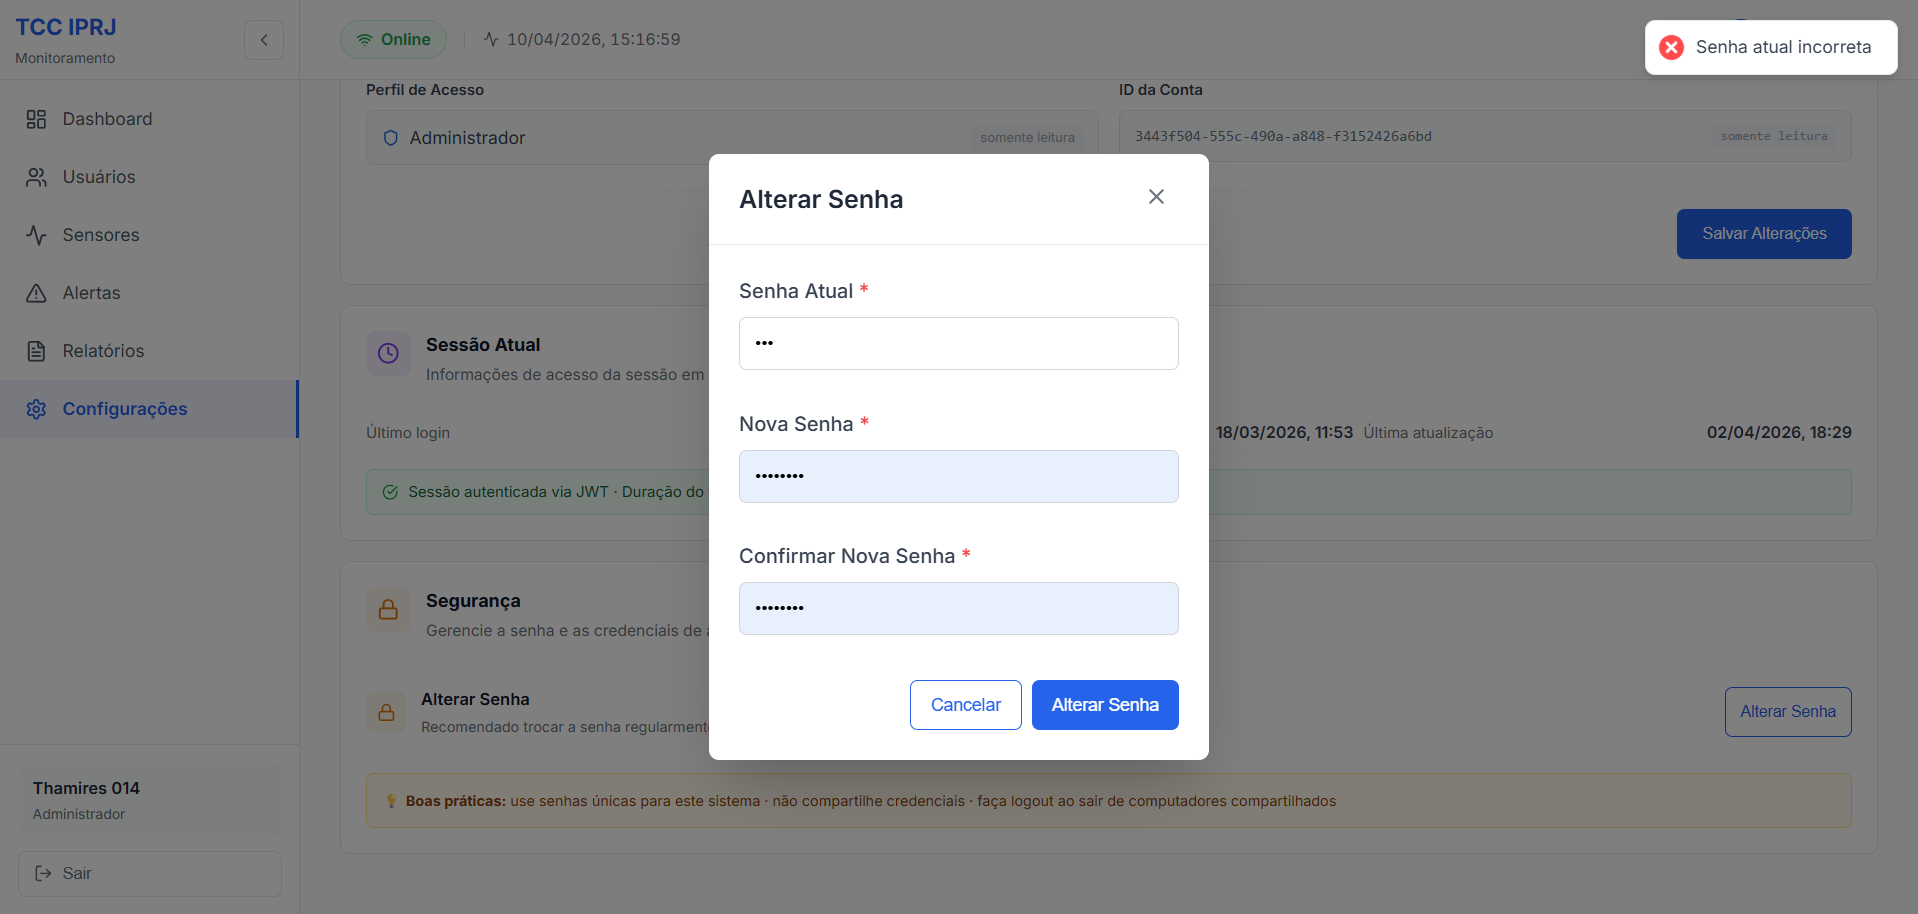
\includegraphics[width=0.75\textwidth]{figures/cap5_alterar_senha_atual_incorreta.png}
    \label{fig:alterar_senha_atual_incorreta}
    \fonte{Elaborado pela autora.}
\end{figure}

% =============================================================
\section{Cobertura dos Objetivos Específicos}
\label{sec:cobertura}
% =============================================================

A \autoref{tab:cobertura_objetivos} relaciona cada objetivo específico
definido no \autoref{cap:objetivos} ao resultado observado no sistema
implementado.

\begin{table}[htb]
\centering
\caption{Cobertura dos objetivos específicos pelos resultados implementados}
\label{tab:cobertura_objetivos}
\begin{tabular}{p{0.04\textwidth}p{0.43\textwidth}p{0.45\textwidth}}
\hline
\textbf{Obj.} & \textbf{Objetivo específico} & \textbf{Resultado observado} \\
\hline
a & Protótipo ESP8266 com higrômetro, LEDs e \textit{buzzer} proporcional
ao risco &
Protótipo montado e em operação; LEDs acendem no nível correspondente;
\textit{buzzer} soa com frequência e cadência crescentes conforme a
gravidade do índice (80--84\%, 85--89\% e $\geq$90\%) \\
\hline
b & Integração com BNDMET/DECEA e OpenWeatherMap para precipitação
histórica e previsão &
Ambas as APIs integradas e em operação; acumulados de 24h, 7d e 30d via
BNDMET e previsão de 24h via OWM; proteção pré-NTP e \textit{retry}
acelerado implementados \\
\hline
c & Modelo de sete variáveis ponderadas com mecanismo de amplificação
$\times 1{,}20$ &
Modelo em operação; todos os sete componentes calculados e exibidos;
amplificação registrada no monitor serial e no \textit{dashboard};
protocolo de ruptura com \textit{cooldown} de três leituras validado \\
\hline
d & \textit{Backend} Node.js com banco de séries temporais e API
RESTful para recebimento, validação e persistência das leituras &
\textit{Backend} em operação com PostgreSQL e TimescaleDB; dados
recebidos, validados e persistidos; 41 campos por leitura;
autenticação JWT funcional \\
\hline
e & Interface \textit{web} com histórico, alertas, meteorologia e
gestão de usuários &
Seis telas implementadas e funcionais: \textit{dashboard}, Sensores,
Alertas, Relatórios, Usuários e Configurações; todos os fluxos de
sucesso e alternativos validados \\
\hline
f & Sistema de envio de alertas por e-mail acionado manualmente pelo
administrador, com formulário de composição, seleção de destinatários
por perfil e registro de auditoria &
Central de alertas operacional com formulário de composição, seleção
de destinatários por perfil, envio em massa e registro de auditoria
por disparo; e-mail HTML colorido por criticidade entregue aos
destinatários \\
\hline
\end{tabular}
\fonte{Elaborado pela autora.}
\end{table}

% =============================================================
\section{Discussão dos Resultados}
\label{sec:discussao}
% =============================================================

Os resultados alcançados confirmam a viabilidade técnica e econômica
da solução proposta. O custo total do protótipo de \textit{hardware}
--- R\$~70,30 --- é expressivamente inferior ao de instrumentos
geotécnicos profissionais como piezômetros elétricos automatizados e
inclinômetros de corda vibrante, cujos valores de aquisição e instalação
podem superar dezenas de milhares de reais por ponto de monitoramento
\cite{quispe2018instrumentacao}. Tecnologias de baixo custo, quando bem
integradas, são capazes de produzir fluxo contínuo de dados geotécnicos
e meteorológicos --- funcionalidade ausente nos sistemas manuais que
predominavam em Mariana e Brumadinho no momento dos acidentes
\cite{taliberti2025tragedia}.

A abordagem multidimensional do modelo de risco tem respaldo direto
na literatura. \citeonline{rico2008mine} identificaram que 39\% dos
rompimentos documentados resultaram da combinação de múltiplos fatores,
não de uma causa isolada --- o que justifica integrar variáveis
geotécnicas, pluviométricas históricas, prospectivas e atmosféricas em
um único índice. O peso maior atribuído à variável de lençol freático,
correspondente a 40\% do índice, está alinhado à preponderância de
causas de saturação do maciço nos acidentes documentados
\cite{robertson2019feijaoson2019}. A inclusão da pressão atmosférica
como indicador antecipatório representa uma contribuição específica do
modelo, fundamentada no estudo de sistemas de monitoramento integrado
discutido no \autoref{cap1Revisao}.

O índice de confiabilidade auditável diferencia o sistema da maioria
das soluções de baixo custo descritas na literatura, que emitem alertas
sem qualificar a incerteza dos dados subjacentes. Para qualquer leitura
histórica, o administrador pode consultar quais fontes estavam
indisponíveis e qual o impacto quantitativo de cada indisponibilidade
--- propriedade alinhada às recomendações do ICOLD sobre transparência
em sistemas de monitoramento \cite{icold2022tailings}. A decisão de
processar o cálculo de risco integralmente no microcontrolador garante
que a análise continue ocorrendo localmente mesmo diante de falhas de
conectividade, o que é crítico para sistemas destinados a ambientes
industriais remotos.

Seis limitações precisam ser registradas, distribuídas entre o
\textit{firmware}, o modelo de risco e a operação da plataforma.

A primeira é espacial: o modelo atribui 40% do índice de risco à
variável de lençol freático, estimada a partir de um único sensor em
um único ponto do maciço. Barragens de rejeitos reais têm extensão de
centenas de metros, e o nível de umidade varia de um ponto para outro
da estrutura --- regiões próximas a drenos internos ou a camadas de
solo com granulometria diferente podem estar em estados de saturação
completamente distintos do ponto monitorado. Uma leitura isolada não
captura esse comportamento distribuído, e é exatamente essa variação ao
longo de toda a estrutura que determina se ela está estável ou em risco.
Um único ponto de medição, por mais representativo que seja na média,
não oferece essa visão completa \cite{rico2008mine}.

A segunda envolve o sensor e sua calibração. O higrômetro resistivo
FC-28 é um componente voltado a aplicações educacionais: a eletrólise
acelerada nos eletrodos em solo permanentemente úmido compromete sua
longevidade em instalações de longa duração. Agrava essa condição o
fato de que a calibração é feita manualmente via monitor serial, sem
procedimento periódico de verificação contra instrumento de referência
e sem registro de data da última calibração. Com o envelhecimento dos
eletrodos, a curva de resposta se desloca progressivamente, e o sistema
não possui mecanismo para detectar nem sinalizar esse desvio ao
administrador. Em uma implantação real, o sensor deveria ser substituído
por instrumento com certificação metrológica, e o sistema estaria
posicionado como camada complementar à instrumentação geotécnica
convencional prevista pela Lei~n.º~14.066/2020 e pela
NBR~13028:2017 \cite{brasil2020lei14066, abnt2017}.

A terceira é metodológica e incide sobre a formulação do componente de
previsão pluviométrica. O fator~$F_{int}$, que compõe~$V_{ch.fut}$,
é um valor discreto em cinco classes (0,00 / 0,25 / 0,50 / 0,75 /
1,00), o que introduz descontinuidades abruptas no índice: uma previsão
de 4,9\,mm e outra de 0,1\,mm produzem o mesmo fator zero, enquanto
o salto de 4,9\,mm para 5,0\,mm causa um incremento instantâneo de
0,038 no índice, independentemente das demais variáveis. Uma formulação
com interpolação linear dentro de cada faixa, mantendo os valores
extremos atuais como âncoras, reduziria esse efeito sem alterar a
estrutura conceitual do modelo.

A quarta decorre do ciclo de vida do \textit{firmware}. Os buffers
históricos --- o circular de umidade, usado em~$V_{taxa}$, e o de
pressão atmosférica, usado em~$V_{press}$ --- são inicializados com
zeros a cada reinicialização do dispositivo. Reinicializações
involuntárias, por estouro de \textit{heap} ou interrupção de energia,
fazem com que os primeiros ciclos pós-\textit{boot} calculem taxas de
variação e quedas de pressão comparando leituras reais contra zeros
históricos, podendo gerar valores artificialmente elevados para esses
dois componentes até que os buffers completem um ciclo completo ---
período que pode chegar a três horas no caso do histórico de pressão,
dado o intervalo de 30 minutos entre consultas ao OWM.

A quinta diz respeito ao escopo de validação do modelo. Os pesos das
sete variáveis foram definidos com base na literatura técnica
especializada \cite{rico2008mine, robertson2019feijaoson2019}, mas não
passaram por processo de calibração estatística sobre casos históricos
de ruptura em barragens de rejeitos brasileiras. Os limiares de 25\%,
30\%, 50\,mm, 150\,mm e 300\,mm têm respaldo bibliográfico, mas foram
adotados sem ajuste para as características específicas dos rejeitos de
minério de ferro predominantes no contexto de referência. A
representatividade da estação D6594 para um ponto específico de
monitoramento, a localização ideal da sonda no perfil do maciço e a
calibração dos limiares para diferentes tipos de rejeito demandariam
validação geotécnica especializada antes de qualquer aplicação
operacional.

A sexta afeta a operação cotidiana da plataforma. Quando o dispositivo
perde conectividade, os ciclos de leitura são calculados localmente mas
não persistidos para envio posterior --- o que gera lacunas na série
temporal registrada no banco. Além disso, o sistema não emite
notificação automática ao administrador quando o nível de alerta evolui
de AMARELO para VERMELHO: o sino no \textit{header} exibe o
\textit{badge} apenas para quem estiver com o painel aberto no momento
da atualização periódica. Em um cenário operacional real, em que o
responsável pelo monitoramento não permanece continuamente diante da
interface, isso representa um risco de resposta tardia. Conectividade
redundante --- Wi-Fi associada a módulo 4G --- e mecanismos de alerta
proativo por \textit{push} ou SMS mitigariam as duas fragilidades.
